% Modern editorial, markup and figure/layout contributions: CC-BY-SA-4.0.
% Historical text and illustrations: Leonhard Euler (1744), public domain.
% Component scope and upstream attribution: see RIGHTS.md.
% SPDX-License-Identifier: CC-BY-SA-4.0
% Adapted from Foadsf/vintage-latex, examples/01-early-modern-page.tex
% Reference commit 559011918849a3da819912a7c26493071d542df5.
% Changes: warm paper, book title, source-page markers, Euler text,
% mathematical notation, geometry, running heads and vector figure.
\documentclass[11pt,twoside]{article}
\usepackage{fontspec}
\usepackage{amsmath}
\usepackage{unicode-math}
\usepackage[latin,english]{babel}
\usepackage{xurl}
\setmainfont{EBGaramond}[Extension=.otf,UprightFont=*-Regular,ItalicFont=*-Italic,BoldFont=*-Bold,BoldItalicFont=*-BoldItalic,Numbers=Lining,Ligatures=Common]
\setmathfont{Garamond-Math.otf}
\usepackage[a4paper,top=27mm,bottom=29mm,inner=28mm,outer=34mm,marginparwidth=18mm,marginparsep=5mm]{geometry}
\usepackage[tracking=true,protrusion=false,expansion=false]{microtype}
\usepackage{tikz}
\usepackage{graphicx}
\usepackage{marginnote}
\usepackage{needspace}
\usepackage{fancyhdr}
\usepackage{titlesec}
\usepackage{hyperref}
\hypersetup{hidelinks,pdftitle={Euler E65: Methodus inveniendi: complete Latin working edition},pdfauthor={Leonhard Euler; prepared by Ruiyi Zhang}}
\setlength{\parindent}{1.2em}
\setlength{\parskip}{0pt}
\linespread{1.08}
\setlength{\emergencystretch}{2em}
\widowpenalty=10000
\clubpenalty=10000
\displaywidowpenalty=10000
\urlstyle{same}
\raggedbottom
\pagestyle{fancy}
\fancyhf{}
\fancyhead[LE,RO]{\small\thepage}
\fancyhead[RE,LO]{\small\textsc{Euler · Methodus inveniendi}}
\renewcommand{\headrulewidth}{0pt}
\setlength{\headheight}{14pt}
\titleformat{\subsection}[block]{\centering\normalsize\scshape}{}{0pt}{}
\titlespacing*{\subsection}{0pt}{1.0\baselineskip}{0.45\baselineskip}
\newcommand{\sourcepage}[1]{\marginnote{\footnotesize\itshape Orig. p.\,#1}}
\newcommand{\originalsection}[1]{\par\noindent\hypertarget{\sectionnamespace:sec:#1}{}\textbf{#1.}\enspace}
\newcommand{\printerrule}{\par\smallskip\begin{center}\rule{.19\linewidth}{.35pt}\hspace{.45em}\rule{.075\linewidth}{1.05pt}\hspace{.45em}\rule{.19\linewidth}{.35pt}\end{center}\smallskip}

\definecolor{warmpaper}{HTML}{FAF6ED}
\pagecolor{warmpaper}
\allowdisplaybreaks[1]

\usepackage{adjustbox}
\newcommand{\sectionnamespace}{chi}
\newcommand{\bookpart}[3]{\clearpage\def\sectionnamespace{#1}\phantomsection\addcontentsline{toc}{section}{#2}\fancyhead[RE,LO]{\small\textsc{Euler · Methodus inveniendi · #3}}}
\renewcommand{\contentsname}{Conspectus huius editionis}
\begin{document}
\hypersetup{pageanchor=false}
\begin{titlepage}
\centering
\vspace*{0mm}
{\fontsize{34}{40}\selectfont\textls[100]{METHODUS}}\par\medskip
{\Large\textls[170]{INVENIENDI}}\par\medskip
{\huge\textls[70]{LINEAS CURVAS}}\par\bigskip
{\Large Maximi Minimive proprietate gaudentes,}\par\bigskip
{\large\textit{SIVE}}\par\bigskip
{\huge\textls[130]{SOLUTIO}}\par\medskip
{\Large\textsc{problematis isoperimetrici}}\par\medskip
{\large\textls[60]{\textsc{latissimo sensu accepti.}}}\par
\vspace{7mm}
{\large\textit{AUCTORE}}\par\medskip
{\LARGE\textsc{Leonhardo Eulero,}}\par\medskip
{\large\textit{Professore Regio, \& Academiæ Imperialis Scientiarum\\ Petropolitanæ Socio.}}\par
\par\medskip
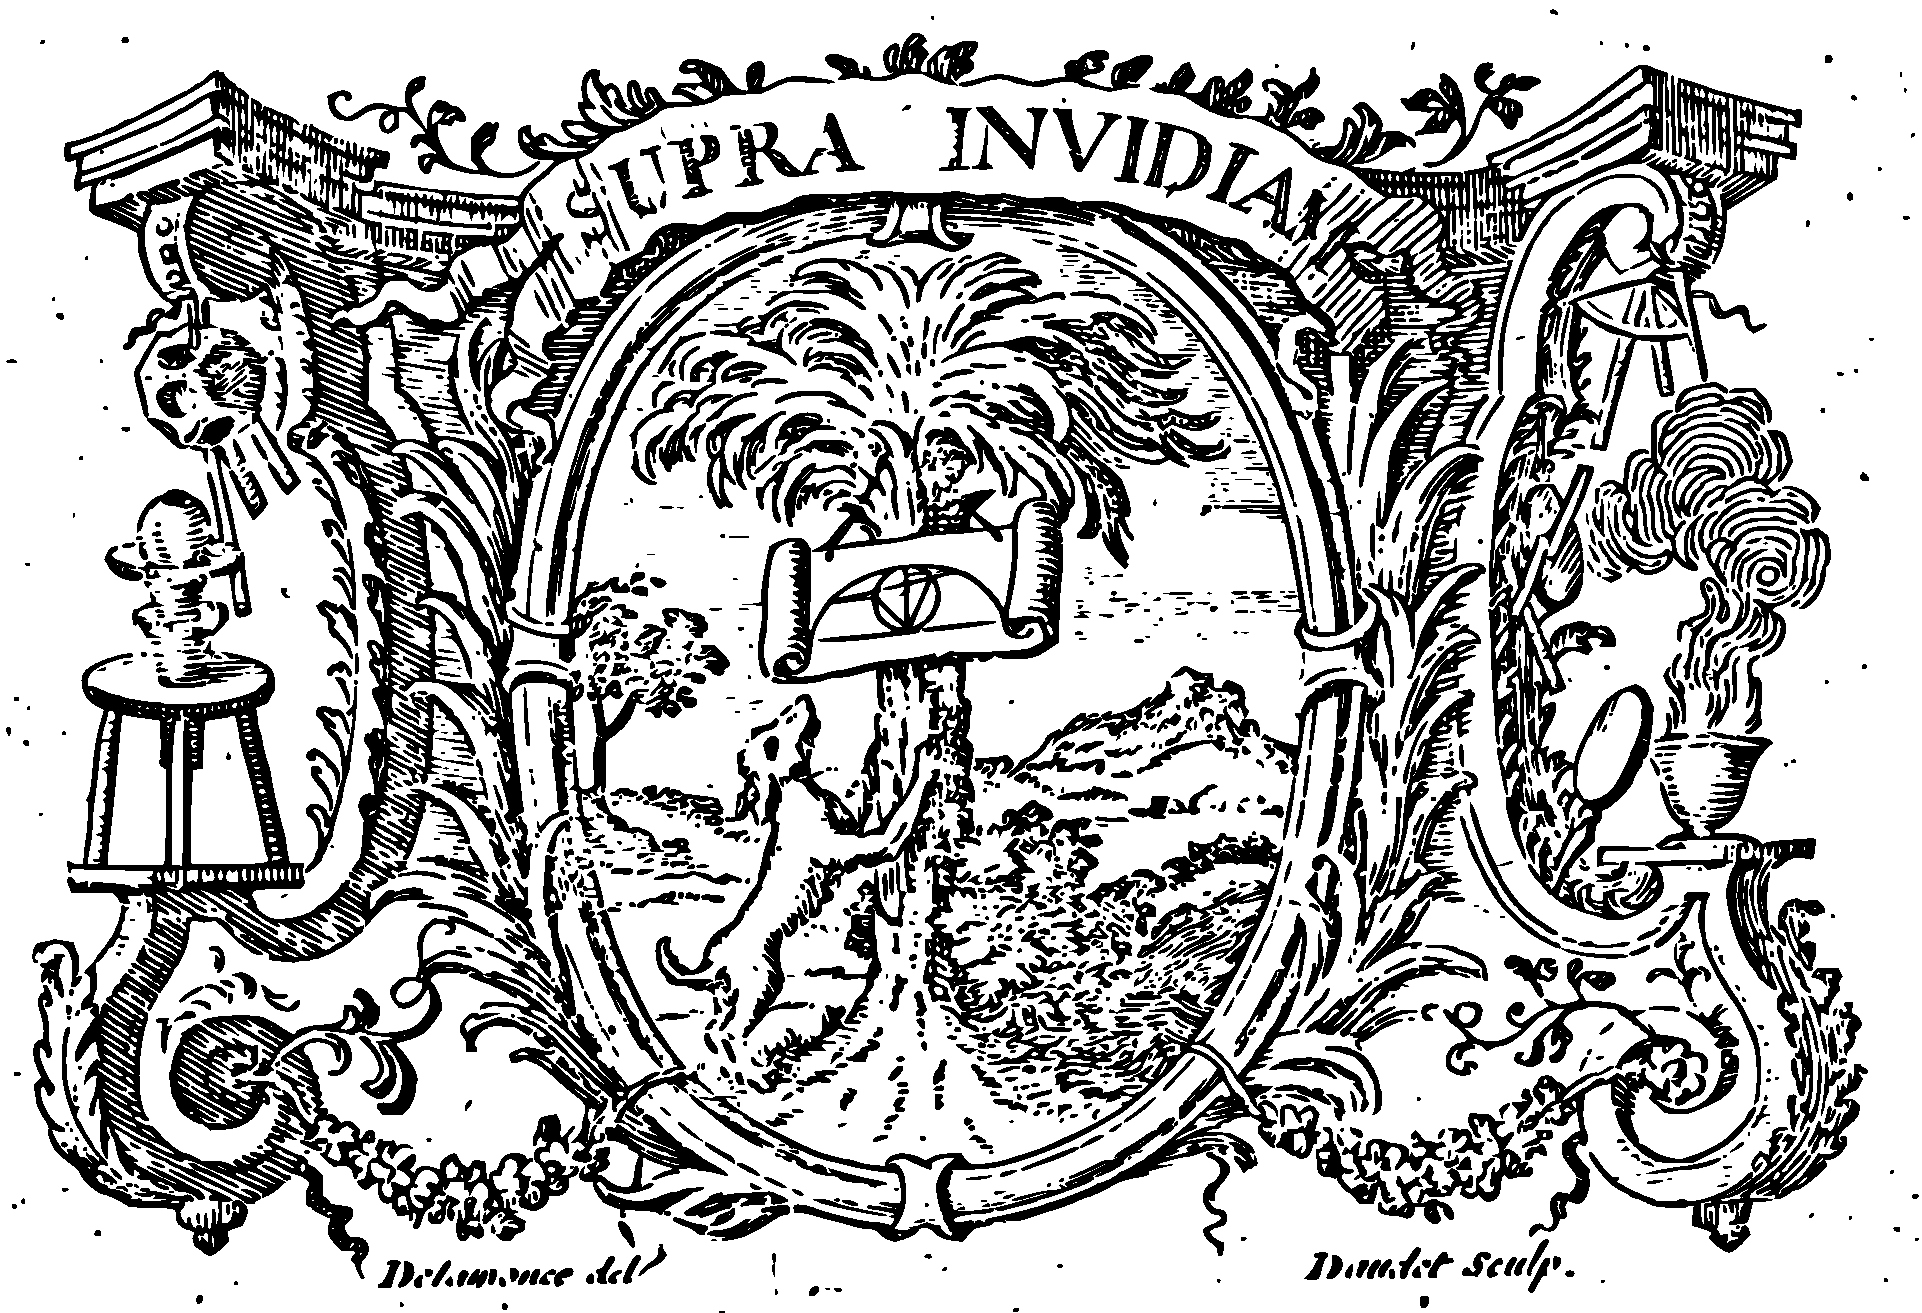
\includegraphics[width=90mm]{figures/title-ornament.pdf}\par\medskip
{\large\textsc{Lausannæ \& Genevæ,}}\par\smallskip
{Apud Marcum-Michaelem Bousquet \& Socios.}\par\medskip
{\large MDCCXLIV.}\par
\vfill
{\large\textsc{Textus Latinus integer}}\par\smallskip
{Capita I–VI · Additamenta I–II · Figuræ}\par\medskip
{Prepared by Ruiyi Zhang · 20 September 2026}\par
{\small Latin transcription and typesetting; editorial draft.}
\end{titlepage}
\setcounter{page}{2}
\hypersetup{pageanchor=true}

\pdfbookmark[0]{Editorial notice}{notice}
\section*{Editorial notice}
This volume brings together all six chapters and both additamenta of Leonhard Euler's 1744 \textit{Methodus inveniendi lineas curvas maximi minimive proprietate gaudentes}, E65. It includes the original index and binder's notice, and all 49 numbered figures. The Latin text and the successive mathematical expressions have been compared with the supplied Euler Archive scan in AI-assisted editorial collation. This is a working edition; independent scholarly collation remains desirable. No Chinese translation is included.

The long s is normalized to s. Line-end divisions, catchwords and printer's signatures are omitted. Original section numbers and source-page markers are retained; page breaks are new. Abbreviated headings may be expanded. Historical notation, including $pp$, $ddy$, proportion-form exponents and successive-value marks, is retained. Suspected source errors are recorded in the accompanying editorial notes and are not silently corrected. Long expressions are broken across lines and grouping delimiters paired for legibility.

The contents on the following page refer to this edition. The original index at the end retains the pagination of 1744. Figure numbers in the six chapters and in the additamenta form two separate sequences. The redrawn figures are grouped at the end for reference; coordinates are schematic and do not assert metric precision.

\subsection*{Title ornament, figures and provenance}
The title ornament is a vector tracing after ETH-Bibliothek Zürich, Rar 4999, \href{https://doi.org/10.3931/e-rara-1490}{doi:10.3931/e-rara-1490}, marked Public Domain. Local brightness separation and Potrace were used. Fine strokes, the motto and signatures were compared visually; faint strokes may still be lost. No missing motifs or lettering have been invented. The numbered figures are vector redrawings after the five plates in the supplied scan. Point names and geometric incidence are retained. The modern redrawings and tracing are not facsimiles of the engraved impressions.

\subsection*{Credits and licensing}
Leonhard Euler's 1744 text is in the public domain. Scan reference: \href{https://scholarlycommons.pacific.edu/euler-works/65/}{Euler Archive, University of the Pacific, E65}. No new rights in the scans are asserted.

Layout adapted from Foadsf/vintage-latex and its contributors, commit \href{https://github.com/Foadsf/vintage-latex/tree/559011918849a3da819912a7c26493071d542df5}{559011918849}, under \href{https://creativecommons.org/licenses/by-sa/4.0/}{CC BY-SA 4.0}. Adaptations include geometry, the warm paper colour (\#FAF6ED), title, source markers, mathematics and vector figures. The adapted template remains under CC BY-SA 4.0.

Text: EB Garamond. Mathematics: Garamond-Math. Both fonts use SIL OFL 1.1. Prepared by Ruiyi Zhang with GPT-6 and delegated assistance, including GPT-5.6 Luna in the earlier chapter work. OCR: Tesseract, Latin language data.
\clearpage
\renewcommand{\contentsname}{Conspectus huius editionis}
\tableofcontents
\clearpage
\selectlanguage{latin}
\bookpart{chi}{Caput I}{Caput I}
% Modern editorial, markup and figure/layout contributions: CC-BY-SA-4.0.
% Historical text and illustrations: Leonhard Euler (1744), public domain.
% Component scope and upstream attribution: see RIGHTS.md.
\sourcepage{1}
\begin{center}
{\Large\textsc{Methodus}}\par\smallskip
{\large\textsc{inveniendi curvas}}\par
{\textsc{maximi minimive proprietate gaudentes.}}
\printerrule
{\Large\textsc{Caput primum.}}\par\medskip
\textit{De Methodo maximorum \& minimorum ad lineas curvas inveniendas applicata in genere.}
\end{center}
\subsection*{Definitio I.}
\originalsection{1}\textit{Methodus maximorum \& minimorum ad lineas curvas applicata}, est methodus inveniendi lineas curvas, quæ maximi minimive proprietate quapiam proposita gaudeant.
\subsection*{Corollarium I.}
\originalsection{2}Reperiuntur igitur per hanc methodum lineæ curvæ, in quibus proposita quæpiam quantitas maximum vel minimum obtineat valorem.

% Modern editorial, markup and figure/layout contributions: CC-BY-SA-4.0.
% Historical text and illustrations: Leonhard Euler (1744), public domain.
% Component scope and upstream attribution: see RIGHTS.md.
\sourcepage{2}
\subsection*{Corollarium II.}
\originalsection{3}Cum autem eadem curva infinitis modis sui similis effici queat, Problema, nisi quædam restrictio adhibeatur, maxime esset indeterminatum, atque adeo nullum. Quæcunque enim curva præbeatur maximi minimive proprietate prædita, semper alia, illi quidem vel similis vel dissimilis, exhiberi posset, quæ illam proprietatem, vel majorem, vel minorem, in se contineret.

\subsection*{Corollarium III.}
\originalsection{4}Quoniam igitur adæquata curvarum cognitio postulat, ut eæ ad axem aliquem positione datum, ejusque portiones quascunque quæ abscissæ vocantur, referantur: prima eaque præcipua restrictio ex quantitate abscissæ petenda erit.

\subsection*{Corollarium IV.}
\originalsection{5}Problemata ergo ad methodum hanc pertinentia ita proponi debent, ut quærantur lineæ curvæ ad axem positione datum relatæ, quæ inter omnes alias curvas eidem abscissæ respondentes maximi minimive proprietate sint præditæ.

\subsection*{Scholion.}
\originalsection{6}Hæc itaque Methodus maximorum \& minimorum maxime discrepat ab illa, quam alibi exposuimus. Ibi enim, pro data ac determinata linea curva, locum determinavimus, ubi proposita quædam quantitas variabilis ad curvam pertinens fiat maxima vel minima. Hic autem ipsa linea curva quæritur, in qua quantitas quædam proposita fiat maxima vel minima. Methodus hæc jam superiori Seculo, mox post inventam Analysin infinitorum, excoli cœpit a Celeb. Fratribus BERNOULLIIS, atque ex eo tempore maxima cepit incrementa. Primum quidem Problema, quod ex hoc genere est tractatum, ad Mechanicam respiciebat, eoque quærebatur linea curva super qua grave descendens citissime delabatur; cui \textit{Curvæ brachystochronæ seu Lineæ celerrimi descensus} nomen erat impositum. In hoc Problemate
\sourcepage{3}
jam manifestum est, id, sine adjuncta conditione, nequidem nomen quæstionis retinere posse: perspicuum enim est, quo brevior magisque ad situm verticalem accedens linea capiatur, eo fore tempus descensus super ea brevius. Quamobrem non absolute quæri potest linea, super qua grave descendens celerrime seu brevissimo tempore delabatur; sed abscissæ quantitas, cui curva invenienda respondeat, simul debuit definiri; ita ut, inter omnes curvas eidem abscissæ in axe positione dato sumtæ respondentes, quæreretur ea super qua corpus grave citissime delaberetur. Neque vero in hoc Problemate ista conditio sufficiebat ad id determinatum efficiendum: sed insuper istam conditionem adjicere oportuit, ut curva invenienda per data duo puncta transeat; atque istud Problema his conditionibus adstringi debuit, ut fieret determinatum, inter omnes, scilicet, lineas curvas per data duo puncta transeuntes eam determinare super qua corpus descendens arcum datæ abscissæ respondentem brevissimo tempore absolvat. Interim tamen hic notandum est, conditionem transitus per duo puncta non esse absolute necessariam, sed in hoc Problemate per ipsam solutionem esse illatam. In solutione enim hujus Problematis immediate pervenitur ad æquationem differentialem secundi gradus, quæ bis integrata duas recipit constantes arbitrarias, ad quas determinandas duobus opus est punctis per quæ curva traducatur, vel aliis similibus proprietatibus: atque hæc eadem conditio, quasi sua sponte, ad omnia istiusmodi Problemata accedit, quarum solutio immediate ad æquationem differentialem secundi gradus deducit. In Problematibus autem quæ resolvuntur per æquationem differentialem quarti vel altioris ordinis, nequidem duo puncta ad curvam determinandam sufficiunt, sed tot opus est punctis, quot gradus differentialia obtinent. Contra vero, si solutio statim ad æquationem algebraicam perducat, tum sine hujusmodi conditione Problema perfecte erit determinatum; dummodo abscissæ longitudo definiatur. Verum hæc omnia clarius perspicientur, quando infra ad solutiones Problematum perveniemus: ibique has notationes fusius explicabimus. Hic enim in principio ista tantum commemorare visum est, ut
\sourcepage{4}
perversas ideas circa determinationem hujusmodi Problematum tollamus.

\subsection*{Definitio II.}
\originalsection{7}\textit{Methodus maximorum ac minimorum absoluta}, docet inter omnes omnino curvas, ad eandem abscissam relatas, determinare eam, in qua proposita quædam quantitas variabilis maximum minimumve obtineat valorem.

\subsection*{Corollarium.}
\originalsection{8}In Problematibus igitur ad hanc methodum pertinentibus, datur axis positione; atque, inter omnes curvas quæ ad hunc axem ejusque determinatam portionem referri possunt, determinatur ea in qua quantitas quædam variabilis sit maxima vel minima.

\subsection*{Scholion.}
\originalsection{9}Aliam conditionem ad maximi minimive determinationem, præter abscissæ quantitatem, hic in genere non adjicimus. Dantur enim Problemata, quæ hoc modo perfecte determinantur; quemadmodum infra distinctius patebit. Etsi enim etiam ejusmodi Problemata occurrunt, ad quæ determinanda insuper duo plurave puncta præscribi possunt, per quæ quæsita curva transeat; tamen hoc demum ex ipsa cujuscunque Problematis solutione perspicietur. Namque si ad ejusmodi æquationem pro curva quæsita perveniatur, in qua per integrationem novæ quantitates constantes sint ingressæ, quæ in ipsa quæstione non inerant; tum solutio censenda erit ambigua, atque vaga; eo quod innumerabiles lineas curvas, quæ ex determinatione illarum quantitatum constantium \& arbitrariarum oriri possunt, in se complectitur. His igitur in casibus erit concludendum, Problema ex sua natura non penitus esse determinatum: sed ad ejus plenam determinationem, præter abscissæ quantitatem, tot novas conditiones adjungi oportere, quibus illæ arbitrariæ constantes ad determinatos valores revocentur. Pro hujusmodi autem conditionibus commodissime assumuntur puncta, per quæ curvæ

% Modern editorial, markup and figure/layout contributions: CC-BY-SA-4.0.
% Historical text and illustrations: Leonhard Euler (1744), public domain.
% Component scope and upstream attribution: see RIGHTS.md.
\sourcepage{5}
quæsitæ sit transeundum; totidem vero puncta, quot insunt in
æquatione inventa quantitates arbitrariæ, ipsam æquationem determinatam
reddent. Loco punctorum autem, ad curvam quæsitam perfecte determinandam,
adhiberi etiam possunt totidem tangentes quæ curvam quæsitam tangant, \&,
si contactus debeat fieri in dato tangentis puncto, hæc conditio duobus
punctis æquivalebit. Quin etiam in locum punctorum, aliæ quæcunque
conditiones substitui possunt; dummodo eæ ita sint comparatæ, ut per eas
quantitates arbitrariæ in æquatione inventa contentæ determinentur.
Neque vero ante opus est solutionem ad finem perducere, quam ista
dijudicatio suscipiatur; sed infra tradentur certa criteria, quorum ope,
statim, ex illa quantitate variabili quæ maximum minimumve esse debet,
dignosci poterit quæ novæ constantes in æquationem pro curva ingrediantur,
quæ in quæstione non continebantur. Oriuntur autem istæ constantes
arbitrariæ ex gradu differentialium, ad quem æquatio pro curva quæsita
exsurgit; quoti enim gradus prodit æquatio differentialis pro curva quæsita,
tot quantitates arbitrariæ in illa censendæ sunt potestate inesse;
hincque totidem conditionibus opus erit ad curvam determinandam. Idem
vero etiam usu venit in solutione omnium Problematum, quando æquatio
differentialis vel primi vel altioris gradus invenitur; ita ut hinc in
præsenti instituto nulla peculiaris difficultas inesse censenda sit.

\subsection*{Definitio III.}
\originalsection{10}\textit{Methodus maximorum ac minimorum relativa} docet, non
inter omnes omnino curvas eidem abscissæ respondentes, sed inter eas tantum
quæ præscriptam quandam proprietatem communem habeant, eam determinare quæ
maximi minimive proprietate gaudeat.

\subsection*{Corollarium I.}
\originalsection{11}Ad hujusmodi igitur Problemata solvenda, primum, ex
omnibus omnino curvis eidem abscissæ respondentibus eæ sunt
\sourcepage{6}segregandæ, in
quas eadem præscripta proprietas competat; atque tum demum ex his segregatis
ea quæ quæritur debebit definiri.

\subsection*{Corollarium II.}
\originalsection{12}Quanquam autem tali conditione numerus curvarum omnium
ad eandem abscissam relatarum vehementer restringitur, tamen is etiamnum
manebit infinitus. Quin etiam, si non una, sed plures proprietates
præscribantur, quibus omnes curvæ ex quibus quæsita est determinanda debeant
esse præditæ, tamen usque numerus curvarum manebit infinitus.

\subsection*{Corollarium III.}
\originalsection{13}Quo plures itaque proponuntur proprietates, quæ iis
curvis ex quibus quæsitam definiri oportet communes esse debeant, eo magis
numerus curvarum inter quas electio quæsita est instituenda restringetur,
etiamsi maneat infinitus.

\subsection*{Scholion I.}
\originalsection{14}Ex hoc genere, in quo Methodum maximorum \& minimorum
relativam constituimus, initio hujus Seculi, primum a Jacobo Bernoullio in
medium prolatum est famosum illud Problema Isoperimetricum; in quo
quærebatur curva maximi minimive proprietate prædita, non inter omnes
curvas ad eandem abscissam relatas, sed inter eas tantum quæ ejusdem
essent longitudinis; ex quo istæ curvæ, ex quibus quæsitam erui oportebat,
isoperimetræ sunt appellatæ. Ita si, inter omnes curvas eidem abscissæ
respondentes \& longitudine æquales, quæratur ea quæ cum abscissa \& applicata
maximum spatium includat; reperitur quæsito linea circularis satisfacere,
quod quidem jam diu ante inventam hanc methodum Geometris innotuerat, ac
demonstratum erat. At, hoc casu iterum, ex ipsa Problematum natura, novæ
conditiones accedunt; uti in iis, quæ ad Methodum maximorum ac minimorum
absolutam pertinent; \sourcepage{7} quæ ex constantibus arbitrariis, quas solutio inducit,
sunt æstimandæ. Ita in solutione Problematis, quo curva quæritur quæ inter
omnes ejusdem longitudinis maximam comprehendat aream cum abscissa, duæ
constantes novæ ingrediuntur; ex quo, ad Problema determinatum efficiendum,
id ita est proponendum, ut inter omnes curvas ejusdem longitudinis, quæ non
solum eidem abscissæ respondeant, sed etiam per data duo puncta transeant,
quæratur ea quæ ad datam abscissam maximam aream referat. Atque simili
modo evenire potest, ut quatuor puncta, \& plura etiam interdum, pro arbitrio
assumi debeant, quo Problema fiat determinatum; cujus rei dijudicatio ex
ipsa Problematum natura est petenda. Quemadmodum autem, in Problemate
isoperimetrico, omnes curvæ ex quibus quæsitam determinari oportet ejusdem
longitudinis ponuntur; ita loco hujus proprietatis alia quæcunque proponi
potest, quæ omnibus communis esse debeat. Sic jam quæsitæ sunt curvæ maximi
minimive proprietate præditæ, inter omnes eas curvas ad eandem abscissam
relatas tantum, quæ circa eam abscissam conversæ omnes æquales superficies
generent; atque simili modo aliæ quæcunque proprietates proponi possunt.
Deinde etiam, non una, sed plures hujusmodi proprietates præscribi possunt,
quæ omnibus curvis inter quas ea quæ maximum minimumve aliquod contineat
definienda sit communes esse debeant. Ita si quæreretur curva maximi vel
minimi proprietate quapiam prædita, inter omnes curvas eidem abscissæ
respondentes, quæ tam essent omnes inter se longitudine æquales, quam etiam
areas æquales concluderent.

\subsection*{Scholion II.}
\originalsection{15}Propter hoc discrimen inter Methodum maximorum \&
minimorum absolutam ac relativam, tractatio nostra erit bipartita. Primum
scilicet methodum trademus, inter omnes omnino curvas eidem abscissæ
respondentes, eam determinandi quæ maximi minimive proprietate sit prædita.
Deinde vero progrediemur ad ejusmodi Problemata, in quibus curva maximi
minimive \sourcepage{8} proprietate gaudens postulatur, inter omnes curvas quæ unam
pluresve propositas proprietates communes habeant; atque ex numero harum
proprietatum istius tractationis denuo subdivisio orietur. Interim tamen
non opus erit in hac subdivisione longius progredi; cum mox reperiatur
methodus, quotcunque etiam propositæ fuerint proprietates, Problemata facile
resolvendi. Solutiones enim Problematum prima fronte maxime intricatorum
præter opinionem fient perquam expeditæ, ac levi calculo absolvendæ.

% Modern editorial, markup and figure/layout contributions: CC-BY-SA-4.0.
% Historical text and illustrations: Leonhard Euler (1744), public domain.
% Component scope and upstream attribution: see RIGHTS.md.
\subsection*{Hypothesis I.}
\originalsection{16}\textit{In hac tractatione abscissam, ad quam omnes curvas referemus, perpetuo littera $x$, applicatam vero littera $y$ designabimus. Tum vero, sumptis elementis abscissæ æqualibus, semper erit}
\[
 dy=pdx;\quad dp=qdx;\quad dq=rdx;\quad dr=sdx;\quad\text{\&c.}
\]
\subsection*{Coroll. I.}
\originalsection{17}His igitur substitutionibus omnia differentialia ipsius $y$ cujuscunque gradus ex expressionibus tollentur, atque præter differentiale $dx$ nulla alia differentialia relinquentur. Quanquam autem hoc modo omnia differentialia, præter $dx$, specie tantum, non revera tolluntur; tamen hæ substitutiones ingens nobis in præsenti instituto afferent subsidium.
\subsection*{Coroll. II.}
\originalsection{18}Quin etiam hujusmodi substitutionibus differentialis constantis assumtio penitus de calculo tollitur: quodcunque enim differentiale aliud constans assumatur, post istas substitutiones perpetuo eadem formula emergere debet. Interim tamen, ob methodum infra adhibendam, necesse erit differentiale $dx$ tanquam constans assumere.
\sourcepage{9}
\subsection*{Coroll. III.}
\originalsection{19}Ut autem facilius appareat, quomodo per has substitutiones differentialia cujusque gradus ipsius $y$ evanescant; juvabit sequentem Tabellam adjecisse.
\[
\begin{aligned}
 dy&=pdx\\
 ddy&=dpdx=qdx^2\\
 d^3y&=dqdx^2=rdx^3\\
 d^4y&=drdx^3=sdx^4\\
 d^5y&=dsdx^4=tdx^5\\
 &\text{\&c.}\qquad\text{\&c.}\qquad\text{\&c.}
\end{aligned}
\]
\subsection*{Coroll. IV.}
\originalsection{20}Quod si etiam arcus curvæ abscissæ $x$ respondens, cum suis differentialibus cujuscunque gradus occurrat; ea omnia per istas litteras ita exprimi poterunt, ut nulla alia differentialia præter $dx$ adsint. Posito enim arcu $=w$ erit.
\[
\begin{aligned}
 w&=\int\sqrt{(dx^2+dy^2)}=\int dx\sqrt{(1+pp)}\\
 dw&=dx\sqrt{(1+pp)}\\
 ddw&=\frac{pqdx^2}{\sqrt{(1+pp)}}\\
 d^3w&=\frac{prdx^3}{\sqrt{(1+pp)}}+\frac{qqdx^3}{(1+pp)^{3:2}}\\
 &\text{\&c.}
\end{aligned}
\]
\subsection*{Coroll. V.}
\originalsection{21}Simili modo, ex his radius osculi seu curvedinis curvæ, in quovis loco, per quantitates specie saltem finitas poterit exprimi. Cum enim, posito elemento $dx$ constante, sit longitudo radii osculi $=\dfrac{-dw^3}{dxddy}$; fiet ea $=\dfrac{-(1+pp)^{3:2}}{q}$.

% Modern editorial, markup and figure/layout contributions: CC-BY-SA-4.0.
% Historical text and illustrations: Leonhard Euler (1744), public domain.
% Component scope and upstream attribution: see RIGHTS.md.
\subsection*{Coroll. VI.}
\originalsection{22}\sourcepage{10}Porro ex iisdem substitutionibus erit, ut sequitur.
\[
\begin{aligned}
\text{Subtangens}&=\frac{y\,dx}{dy}=\frac{y}{p}\\
\text{Subnormalis}&=\frac{y\,dy}{dx}=py\\
\text{Tangens}&=\frac{y\,dw}{dy}=\frac{y\sqrt{(1+pp)}}{p}\\
\text{Normalis}&=\frac{y\,dw}{dx}=y\sqrt{(1+pp)}.
\end{aligned}
\]
Atque, pari modo, omnes quantitates finitæ ad curvam pertinentes, nisi
integralia involvant, per hujusmodi quantitates finitas ita exprimi poterunt,
ut nulla differentialia amplius inesse videantur.

\subsection*{Definitio IV.}
\originalsection{23}\textit{Maximi minimive Formula}, pro quovis Problemate, nobis erit ea quantitas, quæ in curva quæsita maximum minimumve valorem obtinere debet.

\subsection*{Coroll. I.}
\originalsection{24}Quoniam in omnibus Problematibus ad quæ hæc Methodus est accommodata, curva quæritur quæ, vel inter omnes, vel tantum inter innumeras curvas certo modo determinatas, maximi minimive proprietate gaudeat; hæc ipsa proprietas, quæ in curva quæsita maxima vel minima esse debet, erit quantitas; eaque exprimetur Formula, quam maximi minimive Formulam hic appellamus.

\subsection*{Coroll. II.}
\originalsection{25}\sourcepage{11}Cum autem maximi minimive proprietas ita proponi debeat, ut ad datam ac determinatam abscissam referatur; Formula maximi minimive quoque ad illam definitam abscissam debet referri.

\subsection*{Coroll. III.}
\originalsection{26}Erit igitur maximi minimive Formula, quantitas variabilis a longitudine abscissæ cujuscunque cui respondet pendens. Atque in quovis Problemate quæretur curva, pro qua, ad definitam abscissam, illa maximi minimive Formula maximum minimumve obtineat valorem.

\subsection*{Coroll. IV.}
\originalsection{27}Neque vero maximi minimive Formula a sola abscissa pendere potest: hoc enim si esset, pro omnibus curvis eidem abscissæ respondentibus eundem obtineret valorem, atque idcirco omnes æqualiter satisfacerent.

\subsection*{Coroll. V.}
\originalsection{28}Hanc ob rem quoque maximi minimive Formula, præter abscissam omnibus curvis quæ in considerationem veniunt communem, a qualibet curva peculiariter debet pendere; ita ut una sit, pro qua maximum minimumve valorem induere queat.

\subsection*{Scholion I.}
\originalsection{29}\marginpar{\footnotesize\hyperlink{fig:1}{Fig. 1.}}Quo hæc omnia clarius intelligantur, atque status Quæstionum in sequenti pertractandarum melius comprehendatur; ponamus, vel inter omnes omnino curvas, vel tantum inter innumerabiles certam quamdam proprietatem communem habentes, quæ eidem abscissæ $AZ$ respondeant, eam determinari debere,
\sourcepage{12}
pro qua valor formulæ $W$ sit maximus vel minimus. Ponamus huic Quæstioni satisfacere curvam $amz$, ita ut, quæcunque alia curva ad abscissam definitam $AZ$ referatur, valor formulæ $W$ vel fiat minor quam pro hac curva, vel major; prout in curva satisfaciente, $W$ vel maximum esse debet vel minimum. In hac igitur quæstione latissime patente, habemus primo abscissam determinatæ longitudinis $AZ$: deinde curva est quærenda, vel inter omnes omnino curvas ad eandem hanc abscissam relatas, vel tantum inter innumerabiles quibus una pluresve proprietates sint communes, prout quæstio ad methodum maximorum \& minimorum vel absolutam vel relativam est accommodata: tertio habemus eam quantitatem $W$, cujus valor in curva quæsita $amz$ maximus esse debet vel minimus; eritque igitur quantitas $W$ maximi minimive formula, sicut ea est definita. Nunc igitur statim apparet hanc formulam $W$ ita esse debere comparatam, ut ad omnes curvas quæ quidem concipi possunt accommodari queat. Primo scilicet a quantitate abscissæ definitæ $AZ$ debebit pendere; ita ut ea mutetur, valore ipsius $AZ$ mutato. Deinde etiam a natura cujusvis curvæ quæ quidem concipi potest peculiari modo debet pendere: nisi enim ita esset comparata, pro omnibus curvis eundem valorem sortiretur, quæstioque foret nulla. Quamobrem quantitas $W$, præter abscissam, in se quoque complecti debebit quantitates ad curvam ipsam pertinentes. Cum igitur omnis curva determinetur per relationem inter abscissam \& applicatam, quantitas $W$ debet esse conflata ex abscissa \& applicata, \& quantitatibus inde pendentibus. Hoc est, si abscissa indefinita ponatur $=x$, \& applicata respondens indefinita $=y$; quantitas $W$ esse debet functio binarum variabilium $x$ \& $y$. Quod cum ita sit, si curva quæcunque determinata concipiatur, atque ex ejus natura relatio inter $y$ \& $x$ in formula $W$ substituatur, ea definitum impetrabit valorem ad datam illam curvam atque ejus definitam abscissam pertinentem. Quoniam jam, pro aliis atque aliis curvis, formula $W$ diversos valores induit, etiamsi in omnibus abscissa eadem capiatur; manifestum est inter innumerabiles illas curvas \sourcepage{13}unam esse debere in qua valor formulæ $W$ maximus fiat vel minimus; atque ad hanc curvam pro data quacunque determinata quæstione inveniendam, Methodus tradenda est comparata.

\subsection*{Coroll. VI.}
\originalsection{30}Erit igitur maximi minimive formula $W$, functio quædam binarum variabilium $x$ \& $y$: quarum altera $x$ abscissam, altera $y$ applicatam denotat. In $W$ inesse igitur poterunt, non solum ipsæ variabiles $x$ \& $y$, sed etiam omnes quantitates ab iis pendentes, cujusmodi sunt $p$, $q$, $r$, $s$, \&c. quarum significationes supra tradidimus. Quinetiam formulæ integrales ex his ortæ quæcunque in $W$ inesse possunt: imo etiam debent; siquidem quæstio debeat esse determinata, uti mox ostendemus.

\subsection*{Coroll. VII.}
\originalsection{31}Proposita igitur ejusmodi formula $W$, seu functione ipsarum $x$ \& $y$, si quæstio ad methodum maximorum \& minimorum absolutam pertineat, ejusmodi æquatio inter $x$ \& $y$ desideratur, ut, si in $W$ valor ipsius $y$ per $x$ determinatus substituatur, atque ipsi $x$ valor definitus tribuatur; major prodeat quantitas pro $W$, vel minor, quam si ulla alia æquatio inter $x$ \& $y$ assumta fuisset.

\subsection*{Coroll. VIII.}
\originalsection{32}Hoc ergo pacto, quæstiones ad doctrinam linearum curvarum pertinentes ad Analysin puram revocari possunt. Atque vicissim, si hujus generis quæstio in Analysi pura sit proposita, ea ad doctrinam de lineis curvis poterit referri ac resolvi.

\subsection*{Scholion II.}
\originalsection{33}Quanquam hujus generis quæstiones ad puram Analysin \sourcepage{14}reduci possunt, tamen expedit eas cum doctrina linearum curvarum conjungere. Quod si enim animum a lineis curvis abducere, atque ad solas quantitates absolutas firmare velimus; quæstiones primum ipsæ admodum fierent abstrusæ \& inelegantes, ususque earum ac dignitas minus conspiceretur: Deinde etiam methodus resolvendi hujusmodi quæstiones, si in solis quantitatibus abstractis proponeretur, nimium foret abstrusa \& molesta; cum tamen eadem, per inspectionem figurarum \& quantitatum repræsentationem linearem, mirifice adjuvetur atque intellectu facilis reddatur. Hanc ob causam, etsi hujus generis quæstiones, cum ad quantitates abstractas, tum concretas applicari possunt, tamen eas ad lineas curvas commodissime traducemus \& resolvemus. Scilicet quoties æquatio ejusmodi inter $x$ \& $y$ quæritur, ut formula quædam proposita \& composita ex $x$ \& $y$, si ex illa æquatione quæsita valor ipsius $y$ subrogetur, \& ipsi $x$ determinatus valor tribuatur, maxima fiat vel minima: tum semper quæstionem transferemus ad inventionem lineæ curvæ, cujus abscissa sit $x$, \& applicata $y$, pro qua illa formula $W$ fiat maxima vel minima, si abscissa $x$ datæ magnitudinis capiatur. His igitur notatis, natura hujusmodi quæstionum satis luculenter perspicitur: nisi forte cuiquam adhuc dubium creat ambigua locutio de maximo \& minimo simul. Verum ne hic quidem ulla adest ambiguitas; nam etsi methodus ipsa æque monstrat maxima \& minima, tamen in quovis casu facile erit discernere, utrum solutio præbeat maximum an minimum. Sæpe numero autem evenire potest, ut in data quæstione tam maximum quam minimum locum obtineat, atque his casibus solutio erit duplex, altera monstrante maximum, altera minimum. Plerumque autem alterutrum, scilicet vel maximum vel minimum solet esse impossibile; quod evenit, si maximi minimive formula in infinitum vel crescere, vel decrescere potest; his enim casibus, vel non dabitur maximum, vel non minimum. Usu venire etiam potest, ut formula proposita $W$ in infinitum tam crescere quam decrescere queat, atque his casibus nulla prorsus solutio locum \sourcepage{15}habebit. Hæc autem discrimina cuncta ipse calculus post solutionem perpetuo monstrabit.

\subsection*{Propositio I. Theorema.}
\originalsection{34}\textit{Ut per maximi minimive formulam $W$ curva determinetur $amz$, quæ præ omnibus reliquis satisfaciat, formula $W$ debet esse quantitas integralis indefinita, quæ, nisi data assumatur relatio inter $x$ \& $y$, integrari nequeat.}

\subsection*{Demonstratio.}
Ponamus enim formulam $W$ integralia indefinita non involvere; erit ea functio quantitatum $x$ \& $y$, indeque pendentium $p$, $q$, $r$, $s$, \&c. vel algebraica, vel talis transcendens quæ sine assumta relatione inter $x$ \& $y$ exhiberi possit; quod evenit, si vel logarithmi harum quantitatum, vel arcus circulares, vel aliæ hujusmodi quantitates transcendentes definitæ ingrediantur, quæ algebraicis æquivalentes sunt censendæ. Quod si jam $W$ ponatur functio talis ipsarum $x$ \& $y$ tantum, manifestum est valorem formulæ $W$, quem pro data curva $amz$ ad datam abscissam $AZ$ relata obtinet, tantum ab ultima applicata $Zz$ pendere; atque pro omnibus curvis in $Z$ eandem applicatam $Zz$ habentibus fore eundem; atque adeo tali formula $W$ indoles totius curvæ non determinabitur, sed tantum positio extremi ejus puncti $z$; si in $W$ præter $x$ \& $y$ etiam quantitas $p$ insit, tum præter longitudinem applicatæ $Zz$ positio tangentis curvæ in $z$, seu positio ultimi elementi in $z$ determinabitur. Sin autem insuper $q$ ingrediatur, tum positio binorum elementorum curvæ contiguorum in $z$ determinabitur, \& ita porro. Ex quibus sequitur, si fuerit $W$ functio determinata ipsarum $x$, $y$, $p$, $q$, $r$, \&c. tum per illam tantum curvæ portionem infinite parvam circa extremitatem $z$ determinari; atque pro omnibus curvis in eandem extremitatem desinentibus eundem valorem ipsius $W$ esse proditurum. Ut itaque per formulam $W$ tota curva $amz$, quatenus toti abscissæ $AZ$ respondet, definiatur, \sourcepage{16}formulam $W$ ita oportet esse comparatam, ut ejus valor ad determinatam curvam $amz$ applicatus, a positione singulorum elementorum hujus curvæ intra terminos $a$ \& $z$ sitorum pendeat. Hoc autem evenire non potest, nisi quantitas $W$ sit formula integralis indefinita, quæ generatim sine assumta æquatione inter $x$ \& $y$ integrationem non admittat. Q. E. D.

\subsection*{Coroll. I.}
\originalsection{35}Nisi igitur maximi minimive formula $W$ sit quantitas integralis indefinita, nequidem linea curva in qua valor ipsius $W$ sit maximus vel minimus determinabitur; atque adeo quæstio de invenienda curva, in qua esset $W$ maximum vel minimum erit nulla.

\subsection*{Coroll. II.}
\originalsection{36}Ut igitur curva assignari possit, in qua valor ipsius $W$ præ aliis sit maximus vel minimus, formula $W$ talem formam $\int Z\,dx$ habere debet; atque quantitatem $Z$ ita comparatam esse oportet ut differentiale $Z\,dx$, nisi æquatio statuatur inter $x$ \& $y$, integrari nequeat.

\subsection*{Scholion.}
\originalsection{37}Quoniam maximi minimive formula $W$ debet esse integrale formulæ differentialis indefinitæ primi gradus; hoc est cujus integrale fiat quantitas finita; ea formula differentialis semper ad hujusmodi formam $Z\,dx$ poterit reduci, ope litterarum $p$, $q$, $r$, \&c. Et hanc ob rem in sequentibus maximi minimive formula perpetuo per $\int Z\,dx$ nobis indicabitur. Erit autem $Z$ functio non solum quantitatum $x$ \& $y$, sed etiam continebit litteras $p$, $q$, $r$, \&c. Ita si area $AazZ$ debeat esse maxima vel minima, formula $W$ abibit in $\int y\,dx$; \& si superficies solidi rotundi quod generatur rotatione curvæ $amz$ circa axem $AZ$ debeat esse maxima vel minima, erit $W=\int y\,dx\sqrt{(1+pp)}$;

% Modern editorial, markup and figure/layout contributions: CC-BY-SA-4.0.
% Historical text and illustrations: Leonhard Euler (1744), public domain.
% Component scope and upstream attribution: see RIGHTS.md.
% 校录范围：原印刷页 17--23（PDF 页 20--26）。
\sourcepage{17}
atque ita porro quæcunque formula debeat in curva quæsita esse maxima vel minima, ea semper erit hujus formæ $\int Z\,dx$, scilicet integrale quantitatis finitæ cujusdam $Z$ in differentiale $dx$ ductæ. Debet autem $Z$ ejusmodi esse quantitas, ut si æquatio statuatur inter $x$ \& $y$, integrale $\int Z\,dx$ determinatum obtineat valorem: ex quo $Z$ erit functio quantitatum $x$, $y$, \& inde pendentium $p$, $q$, $r$, \&c. vel algebraica sive determinata, vel præterea ipsa in se complectetur formulas integrales indeterminatas; quod discrimen probe est tenendum. Ita si maximi minimive formula $W$ fuerit $\int y\,dx$, vel $\int y\,dx\sqrt{(1+pp)}$; quantitas $Z$ erit algebraica, at si sit $W=\int yx\,dx\int y\,dx$, tum erit $Z=yx\int y\,dx$, hoc est ipsa quantitas $Z$ erit indeterminata, cujus valor nisi relatio inter $x$ \& $y$ detur, exhiberi nequit. Quin etiam evenire potest, ut valor ipsius $Z$ hujusmodi formula evoluta exprimi nequeat, sed tantum per æquationem differentialem demum erui debeat, ut si fuerit $dZ=y\,dx+ZZ\,dx$; ex qua æquatione valor ipsius $Z$ per $x$ \& $y$ nequidem exhiberi potest. Hinc igitur tria nascuntur genera formularum $\int Z\,dx$, quæ in curvis quæsitis maxima vel minima fieri debent. Quorum primum eas complectitur formulas, in quibus $Z$ est functio algebraica seu determinata ipsarum $x$, $y$, \& $p$, $q$, $r$, \&c. Ad secundum genus referimus eas formulas, in quibus quantitas $Z$ ipsa insuper formulas integrales involvit. In tertio autem genere continentur eæ formulæ, in quibus valor ipsius $Z$ per æquationem differentialem, cujus integratio non constat, determinatur.

\subsection*{Propositio II. Theorema.}
\originalsection{38}\textit{Si fuerit $amz$ curva, in qua valor formulæ $\int Z\,dx$ sit maximus vel minimus, atque $Z$ sit functio algebraica seu determinata ipsarum $x$, $y$, $p$, $q$, $r$, \&c. tum ejusdem curvæ quæcunque portio $mn$ eadem gaudebit prærogativa, ut pro ea ad suam abscissam $MN$ relata, valor ipsius $\int Z\,dx$ sit pariter maximus vel minimus.}

\subsection*{Demonstratio.}
Valor\sourcepage{18} formulæ $\int Z\,dx$ pro abscissa $AZ$ est aggregatum omnium valorum ejusdem formulæ, qui singulis abscissæ $AZ$ portionibus respondent. Quod si ergo abscissa $AZ$ in partes quotcunque, quarum una sit $MN$, divisa concipiatur, atque ad singulas partes hasce valor formulæ $\int Z\,dx$ exhibeatur; summa omnium horum valorum præbebit valorem formulæ $\int Z\,dx$, qui toti abscissæ $AZ$ convenit; \& qui erit maximus vel minimus. Quoniam autem $Z$ ponitur functio algebraica ipsarum $x$, $y$, $p$, $q$, \&c. valor formulæ $\int Z\,dx$ respondens abscissæ portioni $MN$, a sola portionis curvæ respondentis $mn$ indole pendebit, idemque manebit, utcunque reliquæ partes $am$ \& $nz$ varientur; singularum enim litterarum $x$, $y$, $p$, $q$, \&c. valores per solam curvæ portionem $mn$ determinantur. Si ergo formulæ $\int Z\,dx$ valores, qui conveniunt abscissæ portionibus $AM$, $MN$, $NZ$, ponantur $P$, $Q$ \& $R$, quantitates hæ $P$, $Q$, \& $R$, a se mutuo non pendebunt. Quare cum earum aggregatum $P+Q+R$ sit maximum vel minimum, etiam unaquæque maximi minimive proprietate prædita sit necesse est. Hanc ob rem, si in curva $amz$ formula $\int Z\,dx$ maximum minimumve habeat valorem, \& quantitas $Z$ sit functio algebraica ipsarum $x$, $y$, $p$, $q$, \&c. tum etiam, pro qualibet illius curvæ portione, eadem formula $\int Z\,dx$ maximi minimive proprietate gaudebit. Q. E. D.

\subsection*{Coroll. I.}
\originalsection{39}Quod si ergo curva fuerit inventa $amz$, quæ pro abscissa data $AZ$, habeat valorem formulæ $\int Z\,dx$ maximum vel minimum, atque $Z$ sit functio algebraica seu determinata, tum etiam ejusdem curvæ qualibet portio, respectu abscissæ suæ respondentis, eadem maximi minimive proprietate gaudebit.

\subsection*{Coroll. II.}
\originalsection{40}\sourcepage{19}In hujusmodi igitur Problematibus, ubi tale maximum minimumve quæritur, non opus est quantitatem abscissæ, cui maximum minimumve respondeat, definire; sed si, pro una quacunque abscissa, formula $\int Z\,dx$ sit maximum vel minimum, tum eadem pro quacunque alia abscissa eadem proprietate gaudebit.

\subsection*{Coroll. III.}
\originalsection{41}Hujusmodi igitur Problemata resolventur, si singulæ curvæ quæsitæ particulæ ita determinentur, ut pro iis valor formulæ $\int Z\,dx$ fiat maximus vel minimus. Tum enim simul tota curva, \& quæcunque ejus portio, pariter eadem maximi minimive proprietate erit instructa.

\subsection*{Scholion.}
\originalsection{42}Proprietas hæc, qua gaudent curvæ in quibus istiusmodi formulæ $\int Z\,dx$, ubi $Z$ est functio algebraica seu determinata ipsarum $x$, $y$, $p$, $q$, \&c. sunt maximum vel minimum, est maximi momenti; ea enim innititur universa methodus hujus generis Problemata resolvendi. Ideo autem potissimum hanc Propositionem afferre visum est, ne ea proprietas, quæ his tantum formulis $\int Z\,dx$, ubi $Z$ est functio vel algebraica vel determinata, est propria, omnium omnino formularum quæ proponi possunt communis esse putetur: in sequente enim Propositione demonstrabimus, si in $Z$ insint formulæ integrales; tum eandem proprietatem non amplius locum habere: ex quo simul natura hujusmodi quæstionum clarius intelligetur. Hujus autem præsentis Propositionis demonstratio ex eo petita est fundamento, quod valor formulæ $\int Z\,dx$, siquidem $Z$ est functio vel algebraica vel determinata ipsarum $x$, $y$, $p$, $q$, $r$, \&c. qui convenit cuicunque abscissæ portioni $MN$, a sola curvæ portione respondente $mn$ pendeat, neque a reliqua curva, vel anteriore $am$, vel posteriore $nz$ afficiatur: quæ ratio cessat, si in $Z$ insint \sourcepage{20}formulæ integrales indeterminatæ. Valores enim quantitatum $x$, $y$, $p$, $q$, $r$, \&c. qui pro arcu curvæ $mn$ obtinent, tantum a positione elementorum hujus arcus $mn$, atque elementis aliquot contiguis, quæ arcum finitæ quantitatis non constituunt, pendent; ex quo etiam quantitas ex iis litteris utcunque composita per solam arcus $mn$ indolem determinabitur, nisi adfuerint quantitates integrales, cujusmodi sunt $\int y\,dx$, quæ totam aream anteriorem $AamM$ introduceret, vel $\int dx\sqrt{(1+pp)}$, quæ totum arcum præcedentem $am$ involveret. Hinc igitur distinctius intelligitur, quid per functionem determinatam ipsarum $x$, $y$, $p$, $q$, $r$, \&c. denotare velimus: Functio scilicet determinata ita est comparata, ut, pro quovis loco, a præsentibus valoribus litterarum $x$, $y$, $p$, $q$, \&c. tantum pendeat, neque valores earum anteriores in se complectatur. Functio autem indeterminata est talis, cujus valor in quovis loco, non ex solis valoribus quos hæ litteræ $x$, $y$, $p$, $q$, \&c. in isto loco obtinent determinari potest, sed insuper omnes valores ad sui determinationem requirit, quos istæ litteræ in omnibus locis anterioribus obtinuerunt. Ita patet, omnes functiones algebraicas esse simul determinatas; præterea vero etiam omnes functiones transcendentes, quæ a relatione inter $x$ \& $y$ non pendent, sunt determinatæ, cujusmodi sunt, $l\sqrt{(xx+yy)}$, $e^{p y}$, $A\sin.\frac{p y}{q}$; quarum valores in quovis loco ex valoribus litterarum, quos in hoc solo loco obtinent, assignari possunt. Quando autem in functione quapiam insunt formulæ integrales indeterminatæ, quæ a mutua relatione inter $x$ \& $y$, quam ubique tenent, pendent, tum earum valor, in dato loco, non ex valoribus, quos hæ litteræ in isto loco habent, cognosci potest, sed insuper omnes valores in locis quibusque anterioribus nosse oportet, hoc est generalem relationem inter coordinatas $x$ \& $y$: talesque functiones vocamus indeterminatas; quippe quæ toto cœlo diversæ sunt ab iis, quas determinatas appellavimus.

\subsection*{Propositio III. Theorema.}
\originalsection{43}\sourcepage{21}\textit{Si fuerit $amz$ curva abscissæ $AZ$ respondens, in qua $\int Z\,dx$ sit maximum vel minimum; in $Z$ autem contineantur formulæ integrales indeterminatæ; tum eadem maximi minimive proprietas non cadit in quamlibet curvæ portionem, sed toti tantum curvæ abscissæ $AZ$ respondenti propria erit.}

\subsection*{Demonstratio.} Concipiatur tota curva $amz$, pro qua $\int Z\,dx$ est maximum vel minimum, in duas partes quasvis divisa per applicatam $Mm$; sitque formulæ $\int Z\,dx$ valor conveniens portioni $am$ $=P$, ejusdem autem formulæ valor pro altera portione $mz$ sit $=Q$: pro tota igitur curva $amz$ valor formulæ $\int Z\,dx$ erit $=P+Q$, quem ponimus esse maximum vel minimum. Quo autem omnem ambiguitatem tollamus, totamque rem distinctius proponere queamus; ponamus $P+Q$ esse maximum: quod enim de maximo demonstrabitur, idem de minimo facile intelligetur. Quod si jam valor ipsius $Q$ a valore ipsius $P$ non dependeret, tum aggregatum $P+Q$ maximum esse non posset, nisi simul uterque valor $P$ \& $Q$ seorsim sit maximus. At nostro casu, quo quantitas $Z$ in se continet formulas integrales indeterminatas, valor ipsius $Q$ non tantum a curvæ portione $mz$ ad quam refertur pendebit, sed simul a tota curva anteriore $am$; atque adeo a valore ipsius $P$. Nunc dicimus, ad id ut $P+Q$ sit maximum, non requiri, ut valor ipsius $P$ sit maximus. Ponamus enim portionem curvæ $am$ ita esse comparatam, ut pro ea $P$ sit maximum, \& aliquantillum mutari concipiatur portio curvæ $am$, ita ut valor formulæ $\int Z\,dx$ minor evadat, puta $=P-p$: fieri utique poterit ut ex hac mutatione valor ipsius $Q$ crescat, quod incrementum ponatur $q$: eritque, mutata aliquantillum portione $am$, ita ut pro ea $\int Z\,dx$ non amplius sit maximum, valor formulæ $\int Z\,dx$ pro tota curva $amz =P-p+Q+q$. Cum igitur evenire queat ut sit $q>p$, intelligitur \sourcepage{22}formulam $\int Z\,dx$ pro tota curva $amz$ maximam esse posse, etiamsi maxima non sit pro qualibet portione $am$. Q. E. D.

\subsection*{Coroll. I.}
\originalsection{44}Quando ergo curva fuerit inventa, quæ, pro data abscissa $AZ$, habeat valorem formulæ $\int Z\,dx$ maximum vel minimum, \& $Z$ sit functio indeterminata; tum non sequitur quamlibet curvæ inventæ portionem eadem maximi minimive proprietate fore præditam.

\subsection*{Coroll. II.}
\originalsection{45}In resolutione igitur hujusmodi Problematum, in quibus curva quæritur, quæ pro data abscissa $AZ$ habeat $\int Z\,dx$ maximum vel minimum, perpetuo ad totius abscissæ propositæ quantitatem erit respiciendum, atque maximum vel minimum ad eam tantum, non vero ad ejus quamlibet portionem, accommodari debebit.

\subsection*{Coroll. III.}
\originalsection{46}Maximum igitur hinc patet discrimen, quod inter formulas $\int Z\,dx$, in quibus $Z$ functio est determinata vel indeterminata, intercedit; simulque autem Methodorum diversitas intelligitur, quibus ad resolutiones quæstionum, in quibus hujusmodi formularum maximi minimive valores requiruntur, uti oportebit.

\subsection*{Scholion.}
\originalsection{47}Ex demonstratione hujus Propositionis non quidem necessario sequitur, si pro data abscissa $AZ$ curva habeat formulam $\int Z\,dx$ maximam vel minimam, tum singulas ejus portiones eadem hac prærogativa gaudere; verumtamen satis intelligitur, quoties eadem proprietas in singulas portiones competat, id \sourcepage{23}casu evenire.
Hincque nihilominus summe necessarium est, solutionem perpetuo ad totam propositam abscissam accommodare. Interim tamen, in Problematibus ad methodum relativam pertinentibus evenire potest, ut formulas $\int Z\,dx$, in quibus $Z$ sit functio indeterminata, quasi determinata esset tractare liceat. Hoc scilicet accidit, si inter omnes tantum curvas in quibus formulæ illæ integrales indeterminatæ quæ in $Z$ insunt æquales obtinent valores, ea desideretur, in qua $\int Z\,dx$ sit maximum vel minimum: hoc enim casu formulæ illæ integrales indeterminatæ fieri censendæ sunt determinatæ. Ita si, inter omnes curvas ejusdem longitudinis, determinanda sit ea in qua sit $\int Z\,dx$ maximum vel minimum, atque in $Z$, præter quantitates determinatas, insit arcus curvæ $\int dx\sqrt{(1+pp)}$; hic, quia in omnibus curvis ex quibus quæsitam definire oportet, eundem obtinet valorem, instar functionis determinatæ tractari poterit: Hæc autem cuncta in sequentibus clarius explicabuntur.

\Needspace{14\baselineskip}
\subsection*{Hypothesis II.}
\originalsection{48}\marginnote{\footnotesize\hyperlink{fig:2}{Fig. 2.}}\textit{Si curvæ abscissa $AZ$ in elementa innumerabilia infinite parva \& inter se æqualia dissecetur, cujusmodi sunt $IK$, $KL$, $LM$, \&c. atque portio quæcunque $AM$ vocetur $x$, cui respondeat functio quæcunque variabilis $F$, eandem functionem $F$, quatenus refertur ad puncta abscissæ vel sequentia $N$, $O$, $P$, $Q$, \&c. vel antecedentia $L$, $K$, $I$, \&c. ita denotabimus, ut sit valor ipsius functionis, qui pro puncto $M$ est $=F$, ut sequitur.
\[
\left.\begin{array}{rcl}
\text{pro }N&=&F'\\
\text{pro }O&=&F''\\
\text{pro }P&=&F'''\\
\text{pro }Q&=&F^{\mathrm{iv}}\\
\text{pro }R&=&F^{\mathrm{v}}\\
&\text{\&c.}
\end{array}\right\}
\qquad\text{pro punctis abscissæ sequentibus}
\]}


% Modern editorial, markup and figure/layout contributions: CC-BY-SA-4.0.
% Historical text and illustrations: Leonhard Euler (1744), public domain.
% Component scope and upstream attribution: see RIGHTS.md.
\sourcepage{24}
\[
\left.\begin{array}{rcl}
\text{pro }L&=&F_{\prime}\\
\text{pro }K&=&F_{\prime\prime}\\
\text{pro }I&=&F_{\prime\prime\prime}\\
\text{pro }H&=&F_{\mathrm{iv}}\\
&\text{\&c.}
\end{array}\right\}
\quad\text{\textit{pro punctis abscissæ antecedentibus.}}
\]
\textit{Atque hoc pacto, sine prolixa differentialium scriptione, valor functionis cujuscunque variabilis, qui in quovis abscissæ puncto locum obtinet, commode indicabitur.}

\subsection*{Corollarium I.}
\originalsection{49}Cum igitur functionis cujusque valor, in loco quocunque, sit æqualis suo valori in loco antecedente differentiali suo aucto, erit
\[
\begin{array}{rclcrcl}
F'&=&F+dF&&F&=&F_{\prime}+dF_{\prime}\\
F''&=&F'+dF'&&F_{\prime}&=&F_{\prime\prime}+dF_{\prime\prime}\\
F'''&=&F''+dF''&&F_{\prime\prime}&=&F_{\prime\prime\prime}+dF_{\prime\prime\prime}\\
F^{\mathrm{iv}}&=&F'''+dF'''&&F_{\prime\prime\prime}&=&F_{\mathrm{iv}}+dF_{\mathrm{iv}}\\
\multicolumn{3}{c}{\&c.}&&\multicolumn{3}{c}{\&c.}
\end{array}
\]

\subsection*{Corollarium II.}
\originalsection{50}Si ex singulis abscissæ divisionibus applicatæ ducantur, atque ea quæ abscissæ $AM=x$ respondet, nempe $Mm$, ponatur $=y$, reliquæ tam sequentes quam antecedentes, ita denotabuntur:
\[
\begin{array}{rlcrl}
Mm&=y&&Mm&=y\\
Nn&=y'&&Ll&=y_{\prime}\\
Oo&=y''&&Kk&=y_{\prime\prime}\\
Pp&=y'''&&Ii&=y_{\prime\prime\prime}\\
Qq&=y^{\mathrm{iv}}&&Hh&=y_{\mathrm{iv}}\\
\multicolumn{2}{c}{\&c.}&&\multicolumn{2}{c}{\&c.}
\end{array}
\]

\subsection*{Corollarium III.}
\originalsection{51}\sourcepage{25}Cum deinde valor ipsius $p$ sit $=\dfrac{dy}{dx}=\dfrac{Nn-Mm}{dx}$; erit $p=\dfrac{y'-y}{dx}$; sequentes autem pariter ac antecedentes ipsius $p$ valores ita se habebunt:
\[
\renewcommand{\arraystretch}{1.8}
\begin{array}{rclcrcl}
p&=&\dfrac{y'-y}{dx}&&p&=&\dfrac{y'-y}{dx}\\
p'&=&\dfrac{y''-y'}{dx}&&p_{\prime}&=&\dfrac{y-y_{\prime}}{dx}\\
p''&=&\dfrac{y'''-y''}{dx}&&p_{\prime\prime}&=&\dfrac{y_{\prime}-y_{\prime\prime}}{dx}\\
p'''&=&\dfrac{y^{\mathrm{iv}}-y'''}{dx}&&p_{\prime\prime\prime}&=&\dfrac{y_{\prime\prime}-y_{\prime\prime\prime}}{dx}\\
\multicolumn{3}{c}{\&c.}&&\multicolumn{3}{c}{\&c.}
\end{array}
\]

\subsection*{Corollarium IV.}
\originalsection{52}Deinde, quia est $q=\dfrac{dp}{dx}=\dfrac{p'-p}{dx}$ erit
\[
q=\frac{y''-2y'+y}{dx^2},
\]
ex quo quantitatis $q$ valores, cum sequentes tum antecedentes, ita se habebunt:
\[
\renewcommand{\arraystretch}{1.8}
\begin{array}{rclcrcl}
q&=&\dfrac{y''-2y'+y}{dx^2}&&q&=&\dfrac{y''-2y'+y}{dx^2}\\
q'&=&\dfrac{y'''-2y''+y'}{dx^2}&&q_{\prime}&=&\dfrac{y'-2y+y_{\prime}}{dx^2}\\
q''&=&\dfrac{y^{\mathrm{iv}}-2y'''+y''}{dx^2}&&q_{\prime\prime}&=&\dfrac{y-2y_{\prime}+y_{\prime\prime}}{dx^2}\\
\multicolumn{3}{c}{\&c.}&&\multicolumn{3}{c}{\&c.}
\end{array}
\]

\subsection*{Corollarium V.}
\originalsection{53}Simili igitur modo per ista applicatarum signa poterunt \sourcepage{26}valores quantitatum $r$, $s$, $t$, \&c. ut has supra assumsimus, determinari, atque ex figura definiri. Erit scilicet
\[
\begin{aligned}
r&=\frac{y'''-3y''+3y'-y}{dx^3},\\[5pt]
s&=\frac{y^{\mathrm{iv}}-4y'''+6y''-4y'+y}{dx^4},\\[5pt]
t&=\frac{y^{\mathrm{v}}-5y^{\mathrm{iv}}+10y'''-10y''+5y'-y}{dx^5},\\[5pt]
&\text{\&c.}
\end{aligned}
\]
unde harum litterarum valores tam præcedentes quam antecedentes formari possunt.

\Needspace{11\baselineskip}
\subsection*{Corollarium VI.}
\originalsection{54}Quod si autem formula $\int Z\,dx$ ad abscissam $AM=x$ fuerit relata; erit ejus valor sequenti abscissæ elemento $MN=dx$ respondens $=Zdx$. Hincque simili modo formulæ $\int Z\,dx$ valores singulis abscissæ elementis respondentes denotabuntur ut sequitur:
\[
\begin{array}{rclcrcl}
\text{pro }MN&=&Zdx&&\text{pro }MN&=&Zdx\\
\text{pro }NO&=&Z'dx&&\text{pro }LM&=&Z_{\prime}dx\\
\text{pro }OP&=&Z''dx&&\text{pro }KL&=&Z_{\prime\prime}dx\\
\text{pro }PQ&=&Z'''dx&&\text{pro }IK&=&Z_{\prime\prime\prime}dx\\
\multicolumn{3}{c}{\&c.}&&\multicolumn{3}{c}{\&c.}
\end{array}
\]


\subsection*{Corollarium VII.}
\originalsection{55}Si ergo expressio $\int Zdx$ ad abscissam curvæ $AM=x$ pertineat; ejusdem expressionis valor, qui conveniet abscissæ propositæ $AZ$, erit
\[
=\int Zdx+Zdx+Z'dx+Z''dx+Z'''dx+\&c.
\]
in infinitum, donec perveniatur ad ultimum punctum $Z$.

\subsection*{Corollarium VIII.}
\originalsection{56}Si igitur curva inveniri debeat, quæ pro data abscissa $AZ$ \sourcepage{27}valorem formulæ $\int Zdx$ habeat maximum minimumve; tum, posita abscissa quacunque indefinita $AM=x$, efficiendum est ut hæc expressio
\[
\int Zdx+Zdx+Z'dx+Z''dx+Z'''dx+\&c.
\]
usque in $Z$ fiat maxima vel minima.

\subsection*{Scholion.}
\originalsection{57}Quanquam hæc hypothesis tantum pro arbitrio est facta; tamen ista signa maximam afferent utilitatem ad Problemata, quæ ad hanc methodum maximorum \& minimorum pertinent, succincte resolvenda. Plurimum enim valet in hujusmodi negotiis commoda signorum electio, ejusque ope calculus non solum contrahi, sed etiam multo facilior \& expeditior reddi potest. Præstabit autem iste signandi modus longe alteri recepto, quo per differentialia valores functionum variabilium proxime sequentes exprimi solent; eo quod in ipsa resolvendi methodo alius generis differentialia occurrent, quæ cum naturalibus quantitatum variabilium differentialibus facile confundi possent, nisi, ista assumta signandi methodo, naturalia differentialia notatione saltem tollerentur.

\subsection*{Propositio IV. Theorema.}
\originalsection{58}\marginnote{\footnotesize\hyperlink{fig:3}{Fig. 3.}}\textit{Si $amnoz$ fuerit curva ad abscissam datam $AZ$ relata, in qua formula $\int Zdx$ maximum minimumve obtineat valorem; atque alia concipiatur curva $amvoz$ ab ista infinite parum discrepans, tum valor formulæ $\int Zdx$ pro utraque curva erit idem.}

\subsection*{Demonstratio.}
Quando in Analysi formula quæpiam variabilis fit maxima, tum primo crescendo continuo magis ad maximum valorem accedit, deinde vero cum hunc attigit, iterum decrescendo ab eo recedit. Iste autem accessus ad maximum valorem atque recessus ab eodem ita fit, ut dum quantitas proxime ad maximum valorem versatur, tum ejus incrementa ac decrementa \sourcepage{28}momentanea evanescant; hocque idem de minimo est intelligendum. Dantur quidem etiam ejusmodi maxima \& minima, circa quæ incrementa \& decrementa sint infinite magna; verum hujus generis maxima \& minima in præsenti instituto raro locum inveniunt, \& si inveniunt, facile erit ea determinare. Sufficiat igitur notasse circa maximum \& minimum mutationes momentaneas non dari posse finitas. Quod si ergo in curva $amnoz$ expressio $\int Zdx$ maximum minimumve habeat valorem; pro alia curva ejusdem expressionis valor eo magis a maximo minimove recedet, quo magis hæc alia curva ab illa discrepet. Sin autem alia curva infinite parum differat ab illa satisfaciente, tum, pro utraque, formula $\int Zdx$ eundem obtinebit valorem. Hujusmodi autem curvam minime discrepantem concipiemus, si arcum tantum infinite parvum $mno$ infinite parum variari, ejusque loco arcum $mvo$ substitui ponamus. Quamobrem ex curva $az$, pro qua $\int Zdx$ maximum est vel minimum, portionem infinite parvam $mno$ excindi, ejusque loco aliam $mvo$ infinite parum ab illa discrepantem inseri intelligamus; tum valor formulæ $\int Zdx$ qui convenit curvæ $amnoz$ æqualis erit valori, qui convenit curvæ $amvoz$. Q. E. D.

\subsection*{Corollarium I.}
\originalsection{59}Quoniam mutatio debet poni quamminima; non sufficiet arcum $mno$, qui immutari ponitur, accipere infinite parvum, sed etiam deviatio $nv$, præ arcus longitudine $mno$, debet esse infinite parva.

\subsection*{Corollarium II.}
\originalsection{60}Posita igitur tali mutatione in curva, mutatio inde etiam in valore formulæ $\int Zdx$ orietur; quæ autem per demonstrationem erit evanescens. Atque hoc modo ex tali assumta mutatione orietur æquatio, quæ simul curvæ quæsitæ naturam præbebit.

\subsection*{Scholion.}
\originalsection{61}\sourcepage{29}In hac Propositione continetur universa methodus resolvendi Problemata, quibus curva desideratur in qua valor formulæ cujusdam indeterminatæ ut $\int Zdx$ sit maximus vel minimus. Semper enim concipitur portio curvæ infinite parva, uti $mno$, aliquantillum variari in $mvo$, atque tum quæritur differentia valorum quos formula $\int Zdx$, cum pro curva vera $amnoz$, tum pro ficta $amvoz$, sortitur, eaque differentia nihilo æqualis posita dat naturam curvæ quæsitæ. Mutatio autem ista in loco indefinito fieri debet, ut ad totam curvam pertineat, atque ad singula loca pateat. Potest autem ista mutatio utcunque institui, dummodo sit infinite parva, atque vel ad duo vel plura curvæ elementa extendi; semper enim eadem resultare debet æquatio finalis. Interim tamen calculi commoditas postulat, ut mutatio in tam paucis elementis instituatur, quæ sufficiat ad solutionem absolvendam. Ita si, inter omnes omnino curvas eidem abscissæ respondentes, ea determinari debeat, in qua sit $\int Zdx$ maximum vel minimum; tum sufficiet bina tantum curvæ elementa mutata concipere. At si non inter omnes curvas, sed eas tantum quæ unam pluresve expressiones communes habeant, ea definiri debeat in qua quæpiam quantitas sit maxima vel minima; tum mutationem non quamcunque $mvo$ accipere licet, sed talem statui oportet, ut illæ proprietates omnibus curvis communes conserventur. His igitur casibus, duo elementa non sufficient, sed plura accipi debebunt, ut omnibus conditionibus satisfieri queat.

\subsection*{Definitio V.}
\originalsection{62}\textit{Valor Differentialis} datæ maximi minimive formulæ respondens est differentia inter valores, quos hæc formula, cum in ipsa curva quæsita, tum in eadem infinite parum immutata, obtinet.

\subsection*{Corollarium I.}
\originalsection{63}\sourcepage{30}In curva igitur, pro qua data formula, puta $\int Zdx$, maximum minimumve esse debet, hujus formulæ valor differentialis respondens evanescet. Atque hanc ob rem si valor differentialis nihilo æqualis ponatur; habebitur æquatio, qua curvæ quæsitæ natura exprimetur.

\subsection*{Corollarium II.}
\originalsection{64}Ex invento igitur valore differentiali, qui propositæ maximi minimive formulæ respondeat, statim habebitur æquatio exprimens naturam ejus curvæ, in qua formula illa proposita maximum minimumve habeat valorem.

\subsection*{Corollarium III.}
\originalsection{65}Totum igitur negotium ad curvas inveniendas, quæ maximi minimive proprietate gaudeant, eo est reductum, ut pro quaque maximi minimive formula ejus conveniens valor differentialis investigetur.

\subsection*{Scholion.}
\originalsection{66}Cum igitur in genere tradita sit idea non solum naturæ quæstionum, quibus curvæ maximi minimive proprietate præditæ quæruntur, sed etiam methodi, qua ad eas resolvendas uti oporteat, ad ipsam tractationem progrediemur. Ac primo quidem Methodum absolutam, qua curvæ quæruntur quæ inter omnes omnino curvas ad eandem abscissam relatæ maximi minimive proprietate quapiam sint præditæ, trademus. Deinde pergemus ad Methodum maximorum ac minimorum relativam, ad quam tales pertinent quæstiones, quæ non inter omnes curvas datæ abscissæ respondentes, sed eas tantum quæ data quadam communi proprietate una pluribusve gaudent, eam determinari jubent, cui maximi minimive prærogativa quæpiam \sourcepage{31}conveniat. In has autem tractationes natura formulæ $\int Zdx$, quæ maximum minimumve esse debet, ingens discrimen infert, prout $Z$ fuerit functio vel determinata vel indeterminata; quemadmodum jam observavimus.

\bookpart{chii}{Caput II}{Caput II}
% Modern editorial, markup and figure/layout contributions: CC-BY-SA-4.0.
% Historical text and illustrations: Leonhard Euler (1744), public domain.
% Component scope and upstream attribution: see RIGHTS.md.
% 校录范围：原印刷页 31--56（PDF 页 34--59）。拉丁文工作稿。
\subsection*{Caput II.}
\textit{De Methodo maximorum ac minimorum ad lineas curvas inveniendas absoluta.}

\subsection*{Propositio I. Problema.}
\originalsection{1}\sourcepage{31}\textit{Si in curva quacunque $amz$ una applicata quævis $Nn$ augeatur particula infinite parva $nv$; invenire incrementa vel decrementa, quæ singulæ quantitates determinatæ ad curvam pertinentes hinc accipient.} \hyperlink{fig:4}{(Fig.~4.)}

\subsection*{Solutio.}
Quantitates determinatæ ad curvam propositam pertinentes sunt, præter abscissam $x$, quæ non afficitur, hæ $y,p,q,r,s,$ \&c. cum suis derivatis valoribus, quos in locis vel sequentibus vel antecedentibus sortiuntur. Quod si nunc ponamus $AM=x$, \& $Mm=y$, erit $Nn=y'$, hujusque valor per translationem puncti $n$ in $v$ augebitur particula $nv$, reliquæ autem applicatæ $y'',y''',y^{\mathrm{iv}},$ \&c. pariter ac præcedentes $y_{\prime},y_{\prime\prime},y_{\prime\prime\prime},y_{\mathrm{iv}},$ \&c. non afficientur. Cum igitur sola applicata $y'$ crescat particula $nv$, ex Cap. præc. §§51 \& seqq. colligetur quantum incrementum reliquæ quantitates omnes capiant ex incremento solius applicatæ $y'$. Omnes scilicet quantitates, quarum valor pendet ab $y'$, mutationem subibunt, reliquæ vero, quæ ab $y'$ non pendent, manebunt invariatæ. Ita cum sit $p=\dfrac{y'-y}{dx}$, hæc quantitas $p$ crescet particula $\dfrac{nv}{dx}$; at cum sit $p'=\dfrac{y''-y'}{dx}$, hæc quantitas \sourcepage{32}$p'$ decrescet particula $\dfrac{nv}{dx}$. Similique modo reliquarum quantitatum incrementa vel decrementa reperientur, delendo in earum valoribus supra exhibitis omnes valores ipsius $y$, præter hunc $y'$, hujusque loco scribendo $nv$. Hoc modo omnium quantitatum determinatarum, quæ quidem mutationem patiuntur, incrementa in sequenti Tabella congessimus.

\begin{center}
\begin{tabular}{c|c@{\qquad}c|c}
\textit{Quant.}&\textit{Increm.}&\textit{Quant.}&\textit{Increm.}\\ \hline
$y'$&$+nv$&$s_{\prime\prime\prime}$&$+\dfrac{nv}{dx^4}$\\[5pt]
$p$&$+\dfrac{nv}{dx}$&$s_{\prime\prime}$&$-\dfrac{4nv}{dx^4}$\\[5pt]
$p'$&$-\dfrac{nv}{dx}$&$s_{\prime}$&$+\dfrac{6nv}{dx^4}$\\[5pt]
$q_{\prime}$&$+\dfrac{nv}{dx^2}$&$s$&$-\dfrac{4nv}{dx^4}$\\[5pt]
$q$&$-\dfrac{2nv}{dx^2}$&$s'$&$+\dfrac{nv}{dx^4}$\\[5pt]
$q'$&$+\dfrac{nv}{dx^2}$&$t_{\mathrm{iv}}$&$+\dfrac{nv}{dx^5}$\\[5pt]
$r_{\prime\prime}$&$+\dfrac{nv}{dx^3}$&$t_{\prime\prime\prime}$&$-\dfrac{5nv}{dx^5}$\\[5pt]
$r_{\prime}$&$-\dfrac{3nv}{dx^3}$&$t_{\prime\prime}$&$+\dfrac{10nv}{dx^5}$\\[5pt]
$r$&$+\dfrac{3nv}{dx^3}$&$t_{\prime}$&$-\dfrac{10nv}{dx^5}$\\[5pt]
$r'$&$-\dfrac{nv}{dx^3}$&$t$&$+\dfrac{5nv}{dx^5}$\\[5pt]
&&$t'$&$-\dfrac{nv}{dx^5}$\\[5pt]
\end{tabular}
\end{center}
Atque ex hac Tabella etiam ulteriorum quantitatum, si quæ occurrunt, incrementa vel decrementa facile cognosci poterunt. Q. E. I.

\subsection*{Corollarium I.}
\originalsection{2}\sourcepage{33}Cognitis igitur incrementis harum quantitatum primariarum ad curvam pertinentium, inde omnium quantitatum ex iis compositarum incrementa, quæ oriuntur ex aucta applicata $y'$, determinari poterunt, si ratio compositionis spectetur.

\subsection*{Corollarium II.}
\originalsection{3}Harum scilicet quantitatum incrementa exhibita, considerari poterunt tanquam earum differentialia. Atque si proposita fuerit quantitas quæcunque ex illis composita, ejus conveniens incrementum ex translatione puncti $n$ in $v$ ortum invenietur, differentiendo illam quantitatem, \& loco differentialium singularum quantitatum, scribendo ea incrementa, quæ his quantitatibus sunt adcripta.

\subsection*{Corollarium III.}
\originalsection{4}Si igitur habeatur hæc functio $y'\sqrt{(1+pp)}$, cujus incrementum, quod ex translatione puncti $n$ in $v$ oritur fit determinandum; ea functio primum differentietur; unde prodit $dy'\sqrt{(1+pp)}+\dfrac{y' p\,dp}{\sqrt{(1+pp)}}$; hicque loco $dy'$ \& $dp$ scribantur incrementa quantitatibus $y'$ \& $p$ convenientia, nempe $+nv$ \& $+\dfrac{nv}{dx}$; eritque functionis propositæ incrementum $=+nv\sqrt{(1+pp)}+\dfrac{y'p\,nv}{dx\sqrt{(1+pp)}}$.

\subsection*{Corollarium IV.}
\originalsection{5}Expedite igitur per differentiationem functionis cujuscunque incrementum, quod ex incremento $nv$ applicatæ $y'$ oritur, assignari potest; id quod ex inspectione figuræ difficulter \& minime generaliter fieri potest.

\subsection*{Scholion.}
\originalsection{6}\sourcepage{34}Probe notandum est hunc modum incrementa functionum seu quantitatum ex $x,y,p,q,$ \&c. harumque derivatis $y',y'',p',p'',$ \&c. datarum incrementa inveniendi, tantum ad functiones determinatas patere, minime vero ad indeterminatas extendi posse. Quod si enim functio proposita fuerit indeterminata, seu formula integralis indefinita, integrationem neque algebraice neque transcendenter admittens, tum differentiatione nihil consequimur ad ejus incrementum inveniendum. In sequentibus autem, ubi ejusmodi maximi minimive formulas $\int Z\,dx$ sumus contemplaturi, in quibus $Z$ sit functio talis indeterminata, in hujusmodi functionum incrementa sumus inquisituri. Sin autem $Z$ fuerit functio determinata, propositi Problematis solutio sufficere potest ad solutiones Problematum huc pertinentium absolvendas.

\subsection*{Propositio II. Problema.}
\originalsection{7}\textit{Si fuerit $Z$ functio determinata ipsarum $x$ \& $y$ tantum, invenire curvam $az$, in qua valor formulæ $\int Z\,dx$ sit maximus vel minimus.} \hyperlink{fig:4}{(Fig.~4.)}

\subsection*{Solutio.}
Concipiatur abscissa $AZ$, cui maximum minimumve formulæ $\int Zdx$ respondere debet, divisa in innumerabilia elementa æqualia, singula per $dx$ denotanda; positaque abscissa indefinita $AM=x$, \& applicata $Mm=y$, ex formula $\int Zdx$ elemento $MN$ respondebit $Zdx$; atque secundum receptum notandi modum, elemento sequenti $NO$ respondebit $Z'dx$, \& sequentibus elementis $OP,PQ$ \&c. respondebunt valores $Z''dx,Z'''dx,$ \&c. antecedentibus vero elementis $LM,KL,IK$ respondebunt $Z_{\prime}dx,\allowbreak Z_{\prime\prime}dx,\allowbreak Z_{\prime\prime\prime}dx,$ \&c. Quare si curva $az$ sit ea ipsa quæ quæritur, debebit esse $Zdx+Z'dx+Z''dx+\&c.$ una cum \sourcepage{35} $Z_{\prime}dx+Z_{\prime\prime}dx+Z_{\prime\prime\prime}dx+\&c.$ maximum vel minimum. Quod si igitur una applicata $Nn=y'$ augeatur particula $nv$, illa expressio eundem valorem retinere, atque adeo valor differentialis formulæ $\int Zdx$, seu summæ terminorum $Zdx+Z'dx+Z''dx+Z'''dx+\&c.$ una cum $Z_{\prime}dx+Z_{\prime\prime}dx+Z_{\prime\prime\prime}dx+\&c.$ evanescere debet. Singulorum igitur horum terminorum valores differentiales, qui oriuntur ex translatione puncti $n$ in $v$, investigari debebunt; eorumque aggregatum erit valor differentialis formulæ $\int Zdx$ respondens, qui positus $=0$ æquationem pro curva quæsita præbebit. Quoniam autem $Z$ ponitur functio determinata ipsarum $x$ \& $y$, habebit ipsius differentiale $dZ$ hujusmodi formam $Mdx+Ndy$, ita ut sit $dZ=Mdx+Ndy$. Valorum igitur derivatorum ipsius $Z$ differentialia ita se habebunt:
\[
\begin{aligned}
dZ'&=M'dx+N'dy',&dZ_{\prime}&=M_{\prime}dx+N_{\prime}dy_{\prime},\\
dZ''&=M''dx+N''dy'',&dZ_{\prime\prime}&=M_{\prime\prime}dx+N_{\prime\prime}dy_{\prime\prime},\\
&\text{\&c.}&&\text{\&c.}
\end{aligned}
\]
Cum nunc valores differentiales terminorum $Zdx,Z'dx,Z''dx,$ \&c. itemque ipsorum $Z_{\prime}dx,\allowbreak Z_{\prime\prime}dx,\allowbreak Z_{\prime\prime\prime}dx,$ \&c. inveniantur, si hi termini differentientur, atque loco $dy'$ in differentialibus scribatur $nv$; loco omnium reliquorum differentialium vero $0$; manifestum est solum terminum $Z'dx$ habiturum esse valorem differentialem, quoniam in ejus solius differentiali occurrit $dy'$. Scripto itaque $nv$ loco $dy'$, erit termini $Z'dx$ valor differentialis $=N'nv\,dx$, qui simul erit valor differentialis totius formulæ $\int Zdx$; quia reliqui termini præter $Z'dx$ nullam variationem patiuntur. Loco $N'$ autem ponere poterimus $N$, quia est $N'=N+dN$, \& $dN$ præ $N$ evanescit. Pro curva igitur quæsita, in qua sit $\int Zdx$ maximum vel minimum, ista habetur æquatio $Ndx\,nv=0$ seu $N=0$; existente $dZ=Mdx+Ndy$. Q. E. I.

\subsection*{Corollarium I.}
\originalsection{8}\sourcepage{36}Si igitur curva debeat definiri, in qua sit $\int Zdx$ maximum vel minimum, atque $Z$ sit functio determinata ipsarum $x$ \& $y$ tantum; tum quantitatem $Z$ differentiare oportet; quod cum habiturum sit hujusmodi formam $dZ=Mdx+Ndy$, hinc formabitur æquatio pro curva quæsita, quæ erit $N=0$.

\subsection*{Corollarium II.}
\originalsection{9}Cum ergo $N$ sit functio ipsarum $x$ \& $y$ determinata, in æquatione pro curva $N=0$ nulla inerit quantitas constans, quæ non fuit in formula maximi minimive $\int Zdx$; \& hanc ob rem curva inventa erit unica \& perfecte determinata.

\subsection*{Corollarium III.}
\originalsection{10}In quæstionibus igitur sub hoc Problemate comprehensis, curva satisfaciens ex sola maximi minimive formula determinatur; neque licebit insuper puncta aliqua præscribere, per quæ curva quæsita transeat.

\subsection*{Corollarium IV.}
\originalsection{11}Quod si $Z$ fuerit functio tantum ipsius $x$, ita ut $y$ non involvat; erit tum $\int Zdx$ functio determinata pariter ipsius $x$ tantum; eique adeo omnes curvæ eidem abscissæ respondentes æque satisfacient. Idem vero hoc modo demonstrat calculus; hoc enim casu, quo in $Z$ non inest $y$, fiet $N=0$; ideoque nulla prodit æquatio pro curva quæsita.

\subsection*{Corollarium V.}
\originalsection{12}Statim etiam intelligi potest, utrum detur linea curva, in qua hujusmodi formula $\int Zdx$ sit maximum vel minimum. Si enim ex differentiatione ipsius $Z$ ejusmodi valor pro $N$ reperiatur, \sourcepage{37}ut per æquationem $N=0$ nulla curva exprimatur; tum etiam nulla curva exstat in qua proposita formula $\int Zdx$ sit maximum vel minimum.

\subsection*{Corollarium VI.}
\originalsection{13}Denique etiam perspicitur, hanc maximi minimive proprietatem non uni alicui determinatæ abscissæ esse adstrictam; sed si curva pro una abscissa reddat formulam $\int Zdx$ maximum vel minimum, eandem pro quacunque alia abscissa pariter maximum minimumve valorem esse habituram.

\subsection*{Scholion I.}
\originalsection{14}Nacti ergo sumus methodum facilem, inter omnes curvas eidem abscissæ respondentes eam determinandi, in qua constituat formula $\int Zdx$ valorem maximum vel minimum, siquidem $Z$ est functio determinata ipsarum $x$ \& $y$ tantum. Simul vero etiam patet curvam satisfacientem semper fore algebraicam, siquidem $Z$ fuerit functio algebraica ipsarum $x$ \& $y$. Curvæ igitur hoc modo inventæ ista erit proprietas, ut si ad eandem abscissam alia quæcunque constituatur linea curva, tum pro ea valor formulæ $\int Zdx$ certo vel minor vel major sit proditurus quam pro inventa, prout in inventa formula $\int Zdx$ vel fuerit maxima vel minima. Cum autem adhuc dubium sit utrum in curva inventa valor formulæ $\int Zdx$ futurus sit maximus an minimus, de eo in quovis casu particulari facile fiet dijudicatio; in genere autem nihil omnino decidi potest. Interim hoc certum est, si unica prodit æquatio, tum tantum vel maximum vel minimum locum habere posse; hoc est, si curva inventa sit pro maximo, tum minimum non dari, sed valorem formulæ $\int Zdx$ in infinitum diminui posse. Pari modo, si unica inventa fuerit curva, in eaque formula $\int Zdx$ sit minima, tum valorem $\int Zdx$ in infinitum augeri posse. Quod si autem solutio nullam prorsus præbeat curvam satisfacientem, id indicio erit valorem formulæ \sourcepage{38}$\int Zdx$ pro quacunque abscissa tam in infinitum crescere quam decrescere posse.

\subsection*{Scholion II.}
\originalsection{15}Ex eadem etiam solutione reperiri poterunt illæ curvæ maximi minimive proprietate præditæ alterius generis supra memoratæ, ad quas non pervenitur per valores differentiales evanescentes, sed infinite magnos; quod maximorum \& minimorum genus ab illo maxime discrepat. Reperientur autem istæ curvæ, si valor differentialis $Ndx\,nv$ non nihilo, sed infinito æqualis ponatur. Quoties igitur hæc æquatio $N=\infty$ lineam aliquam curvam suggerit; tum in ea pariter formula $\int Zdx$ maximum vel minimum obtinebit valorem. Hoc scilicet eveniet, quando pro $N$ prodit fractio, cujus denominator nihilo æqualis positus præbet æquationem pro aliqua linea curva. Hoc itaque pacto plures curvæ reperiri possunt, quæ eidem quæstioni satisfaciant; quarum aliæ maxima continebunt, aliæ minima. Fieri etiam potest, ut plures quam duæ curvæ Problemati satisfacientes reperiantur, etiamsi binæ tantum oriri queant æquationes, scilicet $N=0$ \& $N=\infty$. Si enim $N$ fuerit quantitas ex factoribus composita; tum quilibet factor, vel nihilo vel infinito æqualis positus, dabit æquationem pro curva satisfaciente; constat enim sæpenumero plura maxima pluraque minima locum habere posse. Hæc autem omnia clarius enodabuntur in sequentibus Exemplis in hoc Problemate contentis.

\subsection*{Exemplum I.}
\originalsection{16}\textit{Invenire curvam, quæ, inter omnes omnino curvas eidem abscissæ respondentes, habeat $\int XYdx$ maximum vel minimum; denotante $X$ functionem ipsius $y$, \& $Y$ ipsius $y$ tantum.}
In hoc igitur casu fiet $Z=XY$; ideoque $dZ=YdX+XdY=Mdx+Ndy$. Erit ergo $M=\dfrac{YdX}{dx}$ \& $N=\dfrac{XdY}{dy}$; \& \sourcepage{39}ob $X$ ipsius $x$ \& $Y$ ipsius $y$ functionem. Pro curva igitur quæsita erit $N=\dfrac{XdY}{dy}=0$: quoniam autem $Y$ est functio ipsius $y$, ponatur $dY=\Theta dy$; erit $\Theta$ pariter functio ipsius $y$; ideoque pro curva quæsita, si quæ satisfacit, habetur hæc æquatio $X\Theta=0$, ideoque vel $X=0$, vel $\Theta=0$; quarum cum neutra lineam curvam præbeat, apparet huic quæstioni nullam omnino curvam satisfacere, sed valorem propositum $\int XYdx$ in infinitum cum augeri tum diminui posse. Ex æquatione autem $\Theta=0$, quia $\Theta$ est functio ipsius $y$, sequitur $y=\mathrm{Const.}$ quæ æquatio præbet lineam rectam parallelam abscissæ $AZ$, cujus distantia tanta est, ut fiat functio $Y$ maxima vel minima. Patet enim, si quantitas $Y$ maximum minimumve valorem admittat, tum etiam formulam $\int XYdx$ fieri maximum vel minimum. Altera autem æquatio $X=0$, quia præbet $x=\mathrm{Const.}$ nequidem lineam rectam quæstioni satisfacientem exhibet; quia præbet lineam rectam normalem ad abscissam, quæ propterea non datæ abscissæ cuipiam, sed tantum ejus uni puncto respondebit.

\subsection*{Exemplum II.}
\originalsection{17}\textit{Invenire curvam, quæ, inter omnes eidem abscissæ respondentes curvas, habeat valorem formulæ $\int(ax-yy)y\,dx$ maximum vel minimum.}
Si hæc formula cum generali $\int Zdx$ comparetur, fiet $Z=axy-y^3$, ideoque $dZ=aydx+(ax-3yy)dy$; ita ut fiat $M=ay$ \& $N=ax-3yy$; unde pro curva quæsita habebitur ista æquatio $ax-3yy=0$, seu $yy=\frac13ax$, quæ est pro Parabola verticem in $A$, axem $AZ$ \& parametrum $\frac13a$ habente. In hac igitur Parabola, erit valor formulæ $\int(ax-yy)y\,dx$ maximus vel minimus. Utrum autem sit maximus an minimus, reperietur, si aliam quamcunque lineam loco Parabolæ substituamus, atque inquiramus utrum pro ea valor formulæ propositæ major sit an minor quam pro Parabola. Sumamus \sourcepage{40}igitur lineam rectam cum ipso axe congruentem, pro qua erit $y=0$. Pro hac itaque valor formulæ fiet pariter $=0$, pro Parabola autem idem valor erit affirmativus, ideoque $>0$; ex quo sequitur in Parabola formulæ propositæ valorem non esse minimum, sed maximum. Poterimus autem algebraice indicare quantus futurus sit valor formulæ propositæ pro Parabola: cum enim sit $yy=\frac13ax$, abibit formula proposita in hanc $\int\frac23ax\,dx\sqrt{\frac13ax}=\frac4{15}ax^2\sqrt{\frac13ax}$. Quod si autem ponamus aliam æquationem, puta $y=nx$; abibit formula proposita in hanc $\int dx(naxx-n^3x^3)=\frac13nax^3-\frac14n^3x^4$, quæ semper est minor quam valor formulæ qui pro Parabola inventa prodiit; id quod quilibet facile, substituendis loco $x$ definitis valoribus, experietur.

\subsection*{Exemplum III.}
\originalsection{18}\textit{Invenire curvam, in qua sit, inter omnes omnino curvas ad eandem abscissam relatas, valor hujus formulæ $\int(15a^2x^2y-15a^3xy+5a^2y^3-3y^5)\,dx$ maximus vel minimus.}
Erit igitur $Z=15a^2x^2y-15a^3xy+5a^2y^3-3y^5$, qui si differentietur, posito $x$ constante, prodit $Ndy=15a^2x^2dy-15a^3xdy+15a^2y^2dy-15y^4dy$; hincque $N=15(a^2x^2-a^3x+a^2y^2-y^4)$; qui valor, positus $=0$, dabit æquationem pro curva quæsita: erit itaque $a^2x^2-a^3x+a^2y^2-y^4=0=(ax-yy)(ax+yy-aa)$. Ob binos hos factores, prodeunt binæ curvæ satisfacientes, quarum altera exprimetur hac æquatione $yy=ax$, altera hac $yy=aa-ax$; utraque pro Parabola. Ut nunc appareat utra sit pro maximo vel minimo, ponamus abscissam esse minimam, ac prior æquatio $yy=ax$ in formula substituta dabit $\int -10a^3x\,dx\sqrt{ax}$. Altera vero formula $yy=aa-ax$, seu $y=a$, substituta dabit $\int 2a^5dx$. Quod si autem ipsi $y$ alius quicunque valor tribuatur, puta $y=0$, tum formula proposita abit in $\int0dx=0$. Ex quo patet curvarum inventarum alteram $yy=aa-ax$ esse pro maximo, alteram autem $yy=ax$ pro minimo, scilicet pro maximo negativo. \sourcepage{41}Facillime autem perpetuo hæc dijudicatio, utrum maximum an minimum in curva inventa locum habeat, instituetur, si abscissa $x$ ponatur infinite parva; tum enim integratione non erit opus, sed ipsa formula $Zdx$ monstrabit valorem formulæ $\int Zdx$ hoc casu.

\subsection*{Exemplum IV.}
\originalsection{19}\textit{Inter omnes curvas eidem abscissæ respondentes, definire eam in qua sit formulæ $\int(3ax-3xx-yy)(ax-xx-\frac43xy+yy)\,dx$ valor maximus vel minimus.}
Ex hac igitur formula prodibit sequens ipsius $Z$ valor evolutus:
\[
\begin{aligned}
Z={}&3a^2x^2-4ax^2y+2axyy+\tfrac43xy^3-y^4\\
&-6ax^3+4x^3y-2xxyy+3x^4.
\end{aligned}
\]
quæ differentiata, posito $x$ constante, ac divisa per $dy$, sequentem præbebit valorem pro $N$:
\[
N=-4ax^2+4axy+4xyy-4y^3+4x^3-4xxy.
\]
Quæ expressio, nihilo æqualis posita, dabit æquationem pro curva quæsita. Erit itaque $y^3-xyy+xxy+axx-axy-x^3=0$, quæ duos habet factores, qui totidem præbent æquationes, hasce: I. $y-x=0$, pro linea recta; II. $yy-ax+xx=0$, pro circulo. Ponatur $x$ infinite parva, eritque ex æquatione $y=x$, valor ipsius $Z=3a^2x^2$; at ex æquatione $yy=ax-xx$, seu $y=\sqrt{ax}$, erit $Z=4aaxx$. Quod si autem ponatur $y=a$, prodit $Z=-a^4$, unde apparet utramque lineam inventam esse pro maximo.

\subsection*{Scholion.}
\originalsection{20}\sourcepage{42}Problemata etiam resolvi possunt per Methodum maximorum \& minimorum vulgarem. Quando enim curva quæritur pro qua valor ipsius $\int Zdx$ sit maximus vel minimus, idque pro qualibet abscissa; manifestum est, siquidem $Z$ sit functio determinata ipsarum $x$ \& $y$, formulam $\int Zdx$ maximum minimumve esse non posse, nisi elementum ejus $Zdx$ ac proinde ipsum $Z$ tale sit. Quamobrem quæstioni satisfiet, si quantitas $Z$ differentietur posito $x$ constante, ejusque differentiale ponatur $=0$. Tum enim perpetuo $Z$ habebit valorem maximum vel minimum, ac proinde etiam $Zdx$ \& ipsa formula $\int Zdx$. Quod si autem functio $Z$ differentietur posito $x$ constante, prodit $Ndy$; quoniam generaliter differentiando posuimus $dZ=Mdx+Ndy$; satisfietque ponendo $N=0$: quæ est eadem solutio, quam per Methodum traditam invenimus. Quamvis autem hinc videantur istæ quæstiones simili modo resolvi posse, quo in Methodo maximorum \& minimorum vulgari; tamen hoc tantum evenit, si $Z$ fuerit functio ipsarum $x$ \& $y$ tantum; namque si in $Z$ præterea insint quantitates ex differentialibus ortæ $p,q,r,$ \&c. tum vulgaris Methodus nullius amplius usus esse potest. Etsi enim tum differentietur functio $Z$ posito $x$ constante, tamen in differentiale etiam ingrederentur differentialia $dp,dq,dr,$ \&c. quorum relatio ad $dy$ cum non constet, æquatio inde ad maximum minimumve determinandum apta deduci non poterit. His igitur casibus utilitas \& necessitas nostræ Methodi maxime cernetur.

\subsection*{Propositio III. Problema.}
\originalsection{21}\textit{Si $Z$ fuerit functio ipsarum $x,y,$ \& $p$ determinata, ita ut sit $dZ=Mdx+Ndy+Pdp$; invenire, inter omnes curvas eidem abscissæ respondentes, eam in qua sit $\int Zdx$ maximum vel minimum.} \hyperlink{fig:4}{(Fig.~4.)}

\subsection*{Solutio.}
\sourcepage{43}Sit $amz$ curva quæsito satisfaciens, atque concipiatur applicata quæcunque $Nn=y'$ augeri particula $nv$; debebit valor differentialis formulæ $\int Zdx$, seu quantitatis huic æquivalentis, puta $Zdx+Z'dx+Z''dx+Z'''dx+\&c.$ una cum $Z_{\prime}dx+Z_{\prime\prime}dx+Z_{\prime\prime\prime}dx+\&c.$ esse $=0$. Totius igitur quantitatis $\int Zdx$ valor differentialis ex translatione puncti $n$ in $v$ habebitur, si singulorum illorum terminorum, qui quidem hac translatione afficiuntur, valores differentiales quærantur \& in unam summam addantur. Ex translatione autem puncti $n$ in $v$, illi tantum termini mutationem subeunt, in quibus insunt quantitates $y',p$ \& $p'$; ideoque tantum termini $Zdx$ \& $Z'dx$; nam uti $Z$ est functio ipsarum $y$ \& $p$ præter $x$; ita $Z'$ similis est functio ipsarum $y'$ \& $p'$. Quamobrem hi termini debebunt differentiari, atque in eorum differentialibus loco $dy',dp,$ \& $dp'$ scribi oportet valores supra indicatos $+nv,+\dfrac{nv}{dx}$ \& $-\dfrac{nv}{dx}$. Sicut autem est $dZ=Mdx+Ndy+Pdp$, ita erit $dZ'=M'dx+N'dy'+P'dp'$. Hinc itaque valor differentialis ipsius $Z$ erit $P\dfrac{nv}{dx}$, \& ipsius $Z'$ erit $N'nv-P'\dfrac{nv}{dx}$; ex quo utriusque termini $Zdx+Z'dx$, ideoque integræ formulæ $\int Zdx$ valor differentialis erit $nv\left(P+N'dx-P'\right)$. At est $P'-P=dP$, \& loco $N'$ scribi potest $N$; unde valor differentialis erit $=nv(Ndx-dP)$. Quare cum formulæ $\int Zdx$ valor differentialis nihilo æqualis factus præbeat æquationem pro curva quæsita, hæc erit $0=Ndx-dP$, vel $N-\dfrac{dP}{dx}=0$, qua æquatione natura curvæ quæsitæ exprimitur. Q. E. I.

\subsection*{Corollarium I.}
\originalsection{22}Quod si ergo fuerit $Z$ functio quæcunque ipsarum $x,y$, itemque earum differentialium $dx$ \& $dy$, seu loco horum differentialium, \sourcepage{44}ipsius $p$; existente $dy=pdx$; differentiale ipsius $Z$ hujusmodi habebit formam, ut sit $dZ=Mdx+Ndy+Pdp$. Atque hinc reperietur curva, in qua sit $\int Zdx$ maximum vel minimum, formando hanc æquationem $N-\dfrac{dP}{dx}=0$ seu $Ndx=dP$.

\subsection*{Corollarium II.}
\originalsection{23}Æquatio hæc igitur semper erit differentialis secundi gradus, nisi in $P$ planè non insit $p$. Nam si $p$ contineretur in $P$, tum in $dP$ inerit $dp$; quod ob $p=\dfrac{dy}{dx}$ differentialia secundi gradus involvet.

\subsection*{Corollarium III.}
\originalsection{24}Quando ergo in differentiali ipsius $dZ=Mdx+Ndy+Pdp$ quantitas $P$ adhuc in se complectitur $p$; tum, ob æquationem pro curva quæsita differentialem secundi gradus, duæ novæ constantes arbitrariæ per integrationem ingredientur. Ex quo ad harum constantium determinationem, duo curvæ puncta præscribi poterunt; alias enim non una, sed innumerabiles curvæ reperirentur.

\subsection*{Corollarium IV.}
\originalsection{25}Ut itaque hujusmodi Problemata determinate proponantur, ita sunt enuncianda, ut per data duo puncta curva duci debeat, quæ, inter omnes alias curvas per eadem puncta ductas pro eadem abscissa $x$ valorem $\int Zdx$ maximum minimumve complectatur.

\subsection*{Corollarium V.}
\originalsection{26}In $P$ autem quantitas $p$ non inerit, si $Z$ fuerit functio ipsarum $x$ \& $y$ tantum, per $p$ vel per $n+p$, denotante $n$ numerum \sourcepage{45}constantem, multiplicata. Sit enim $V$ functio ipsarum $x$ \& $y$ tantum; ita ut sit $dV=Mdx+Ndy$; atque $Z=V(n+p)$, erit $dZ=(n+p)Mdx+(n+p)Ndy+Vdp$. Hincque æquatio pro curva quæsita erit $0=(n+p)N-\dfrac{dV}{dx}$, seu $(n+p)Ndx=dV=Mdx+Ndy$.

\subsection*{Corollarium VI.}
\originalsection{27}His igitur casibus, quibus est $Z=V(n+p)$, existente $V$ functione ipsarum $x$ \& $y$ tantum, non pervenitur ad æquationem differentialem secundi gradus: quia $dp$ in ea prorsus non inest. Verum nequidem ad differentialem æquationem primi gradus pervenitur; sed adeo ad algebraicam. Nam cum sit $pdx=dy$, erit $(n+p)Ndx=nNdx+Ndy$; quod ipsi $Mdx+Ndy$ æquale positum, dabit æquationem per $dx$ divisibilem, adeoque algebraicam, hanc $nN=M$, siquidem $V$ fuerit functio algebraica.

\subsection*{Corollarium VII.}
\originalsection{28}Quoties autem hoc evenit, maximi minimive formula, quæ est $\int Zdx$, erit talis formæ $\int(Vn\,dx+V\,dy)$, vel posito $n=0$, talis $\int Vdy$. Hujusmodi igitur maximi minimive formulæ pariter ad æquationem determinatam pro curva quæsita deducunt, ita ut non liceat unum plurave puncta præscribere, per quæ curva transire debeat.

\subsection*{Corollarium VIII.}
\originalsection{29}Posita igitur $V$ functione ipsarum $x$ \& $y$, ista maximi minimive formula $\int Vdy$ pari modo tractatur, quo $\int Vdx$. Nam, posito $dV=Mdx+Ndy$, formulæ $\int Vdx$ respondet æquatio pro curva hæc $N=0$, ita alteri formulæ $\int Vdy$ respondet æquatio $M=0$. Ex quo perspicuum est coordinatas $x$ \& $y$ inter se commutari posse.

\subsection*{Scholion I.}
\originalsection{30}\sourcepage{46}Apparet itaque in solutione hujusmodi Problematum, quibus quæritur curva valorem formulæ $\int Zdx$ maximum minimumve habens, existente $Z$ functione ipsarum $x,y,$ \& $p$, perveniri ad æquationem differentialem secundi gradus, nisi in $Z$ quantitas $p$ unicam tantum habeat dimensionem. Sæpe numero autem ista æquatio differentialis secundi gradus integrationem admittit, de quo in singulis casibus erit videndum. Interim hic annotasse juvabit, generaliter integrationem succedere, si in functione $Z$ omnino non insit $x$, hoc est, si in ejus differentiali $dZ=Mdx+Ndy+Pdp$ valor $M$ evanescat, ita ut sit tantum $dZ=Ndy+Pdp$. Cum enim pro curva inventa sit hæc æquatio $N-\dfrac{dP}{dx}=0$; multiplicetur ea per $dy$, \& quia est $dy=pdx$, ea abibit in hanc $Ndy-pdP=0$, cui æquivalet ista $Ndy+Pdp=Pdp+pdP=dZ$, cujus integrale est $Z+C=Pp$, quæ æquatio jam tantum est differentialis primi gradus. Quoties ergo inter omnes curvas eidem abscissæ respondentes ea quæritur, in qua sit valor formulæ $\int Zdx$ maximum vel minimum, atque $Z$ tantum sit functio ipsarum $y$ \& $p$, ita ut sit $dZ=Ndy+Pdp$; tum pro curva satisfaciente statim exhiberi poterit æquatio differentialis primi gradus ista $Z+C=Pp$. Deinde vero etiam, si $Z$ fuerit functio ipsarum $x$ \& $p$ tantum, atque $dZ=Mdx+Pdp$, evanescente termino $Ndy$, tum pro curva prodibit æquatio differentialis primi gradus. Nam, ob $dP=0$, erit $P=C$, quæ pro curva quæsita dabit æquationem differentialem primi gradus tantum. Quod si autem insuper $M$ evanescat, seu $Z$ functio sit ipsius $p$ tantum, \& $dZ=Pdp$, æquatio inventa $P=C$ transmutabitur in istam $Pdp=Cd p=dZ$, quæ denuo integrata dat $Z+D=Cp$. Hoc autem casu, quia $Z$ \& $P$ sunt functiones ipsius $p$ tantum, utraque æquatio $P=C$ \& $Z+D=Cp$ præbebit pro $p$ valorem constantem; ideoque æquationem hujus formæ $dy=ndx$, quæ indicat hujusmodi Problematis satisfacere \sourcepage{47}lineas rectas, \& quidem quascunque utlibet ductas. Nam in æquatione $P=C$, cum $C$ sit constans arbitraria, valor ipsius $p$ non solum constans, sed etiam arbitrarius evadet; ex quo linea recta quæcunque resultabit. Quamobrem si per data duo puncta curva duci debeat, in qua sit $\int Zdx$ maximum vel minimum, ac $Z$ sit functio ipsius $p$ tantum, tum satisfaciet linea recta per illa data duo puncta ducta.

\subsection*{Scholion II.}
\originalsection{31}Quoniam supra jam vidimus in hujusmodi Problematis coordinatas $x$ \& $y$ inter se commutari, atque, si commodum videatur, applicatam $y$ tanquam abscissam tractari posse, idem hoc quoque casu confirmari juvabit. Sit igitur curva investiganda in qua sit $\int Zdy$ maximum vel minimum, existente $Z$ functione ipsarum $x,y$ \& $p$, \& $dZ=Mdx+Ndy+Pdp$. Hæc autem formula $\int Zdy$ ad nostram formam reducta abit in $\int Zpdx$: in qua erit $d(Zp)=Mpdx+Npdy+(Z+pP)dp$; ex qua formulæ propositæ valor differentialis respondens erit $(Npdx-dZ-Pdp-pdP)nv=(-Mdx-2Pdp-pdP)nv$; \& æquatio pro curva quæsita erit $0=-Mdx-2Pdp-pdP$ seu $0=-Mdy-d(Pp^2)$. Quod si nunc ad similitudinem ostendendam, quia hic $y$ tanquam abscissam consideramus, ponamus $dx=\pi dy$, erit $p=\frac1\pi$ \& $dp=-\dfrac{d\pi}{\pi\pi}=-pp\,d\pi$; erit $dZ=Mdx+Ndy-Ppp\,d\pi=Mdx+Ndy+\Pi d\pi$, ponendo $\Pi=-Ppp$; ut similitudo terminorum conservetur. Quapropter æquatio pro curva erit $0=-Mdy+d\Pi$; quæ eadem æquatio prodiisset, si in formula $\int Zdy$, applicata $y$ in abscissam \& vicissim abscissa in applicatam transmutentur. Proposita igitur quacunque formula indeterminata ex $x$ \& $y$ horumque differentialibus composita, quæ debeat esse maxima vel minima, coordinatarum $x$ \& $y$ utramlibet licebit tanquam abscissam tractare, ad eamque maximum minimumve accommodare.

\subsection*{Exemplum I.}
\originalsection{32}\sourcepage{48}\textit{Inter omnes curvas ad eandem abscissam relatas, eam determinare, in qua sit $\int(Zdx+[Z]dy)$ maximum vel minimum; existentibus $Z$ \& $[Z]$ functionibus quibuscunque ipsarum $x$ \& $y$, ita ut sit $dZ=Mdx+Ndy$ \& $d[Z]=[M]dx+[N]dy$.}
Ut formula hæc $\int(Zdx+[Z]dy)$ ad formam receptam reducatur, ponatur $pdx$ loco $dy$; habebiturque hæc formula $\int(Z+[Z]p)dx$ maxima minimave efficienda. Differentietur ergo valor $Z+[Z]p$; eritque ejus differentiale $=Mdx+Ndy+[M]pdx+[N]pdy+[Z]dp$. Jam per regulam inventam, hinc pro curva quæsita ista prodit æquatio $0=(N+[N]p)dx-d[Z]=(N+[N]p)dx-[M]dx-[N]dy$; quæ, ob $[N]pdx=[N]dy$, per $dx$ divisa dabit hanc æquationem pro curva quæsita algebraicam seu finitam $N-[M]=0$, seu $N=[M]$. Hinc intelligitur si formula proposita $\int(Zdx+[Z]dy)$ fuerit determinata, seu differentiale $Zdx+[Z]dy$ ita comparatum, ut integrationem admittat; tum nullam lineam quæsito esse satisfacturam, seu potius omnes lineas æque satisfacere. Nam si $Zdx+[Z]dy$ integrationem admittit, per se erit $N=[M]$; uti alibi de formulis differentialibus duarum variabilium determinatis demonstravimus; ideoque his casibus prodit æquatio identica $0=0$. Hincque luculenter intelligitur, quod jam ante notavimus, maximi minimive formulam oportere esse formulam indeterminatam; alioquin enim omnes lineæ curvæ æque satisfacerent.

\subsection*{Exemplum II.}
\originalsection{33}\textit{Inter omnes lineas ad eandem abscissam relatas, determinare eam, cujus longitudo sit minima; seu in qua sit $\int dx\sqrt{(1+pp)}$ minimum.}
Primum quidem apparet in hac quæstione maximum non dari, \sourcepage{49}cum linearum longitudo in infinitum augeri queat, manente abscissa eadem. Ita minimum tantum habebit locum, id quod ex ipsa Geometria elementari constat, in qua demonstratur lineam rectam inter omnes alias lineas intra eosdem terminos sitas esse brevissimam. Hoc igitur Exemplum ideo attulisse visum est, cum ut consensus nostræ Methodi cum veritate aliunde jam cognita intelligatur, tum etiam ut circumstantia de duobus punctis arbitrariis, quæ ad hujus generis quæstiones addi debet, melius percipiatur. Erit igitur, formula $\int dx\sqrt{(1+pp)}$ cum generali $\int Zdx$ comparata, $Z=\sqrt{(1+pp)}$, \& $dZ=\dfrac{p\,dp}{\sqrt{(1+pp)}}$; unde fit $M=0,N=0,\&P=\dfrac{p}{\sqrt{(1+pp)}}$. Quare, cum in genere æquatio pro linea quæsita sit $N-\dfrac{dP}{dx}=0$, habebimus hoc casu $dP=0$; ideoque $P=\dfrac{p}{\sqrt{(1+pp)}}=\mathrm{Const.}$ ex qua æquatione oritur $p=\mathrm{Const.}=n$, seu $dy=ndx$, quæ denuo integrata dat $y=a+nx$. Non solum ergo patet lineam quæsitam esse rectam, sed etiam, ob duas arbitrarias constantes $a$ \& $n$, rectam utcunque ductam. Quare si per data duo puncta linea duci jubeatur brevissima, erit illa recta. Similiter autem intelligitur, si linea debeat inveniri, in qua sit $\int Zdx$, ubi $Z$ est functio ipsius $p$ tantum, maximum vel minimum, tum lineam rectam tantum satisfacere; uti ante jam notavimus.

\subsection*{Exemplum III.}
\originalsection{34}\textit{Inter omnes curvas ad eandem abscissam relatas, determinare eam, in qua sit $\int\dfrac{dx\sqrt{(1+pp)}}{\sqrt{x}}$ maximum vel minimum.}
Hæc formula oritur, si quæratur linea celerrimi descensus, in hypothesi gravitatis uniformis, ponendo axem in quo abscissæ capiuntur verticalem. Erit igitur $Z=\dfrac{\sqrt{(1+pp)}}{\sqrt{x}}$ \&
\sourcepage{50}
\[
dZ=-\frac{dx\sqrt{(1+pp)}}{2x\sqrt{x}}+\frac{p\,dp}{\sqrt{x}\sqrt{(1+pp)}};
\]
unde fit $M=-\dfrac{\sqrt{(1+pp)}}{2x\sqrt{x}},\ N=0,\ P=\dfrac{p}{\sqrt{x}\sqrt{(1+pp)}}$. Cum jam curva quæsita exprimatur æquatione $N-\dfrac{dP}{dx}=0$; erit $dP=0$, \& $P\left(=\dfrac{p}{\sqrt{x(1+pp)}}\right)=\mathrm{Const.}=\dfrac1{\sqrt a}$; quæ reducta præbet $ap^2=x+p^2x$, \& $p=\dfrac{dy}{dx}=\sqrt{\dfrac{x}{a-x}}$, seu $y=\int dx\sqrt{\dfrac{x}{a-x}}$, quæ æquatio indicat curvam quæsitam esse Cycloidem super basi horizontali natam, \& cuspidem in suprema axis regione habentem: quæ adeo per data duo quæcunque puncta duci poterit.

\subsection*{Exemplum IV.}
\originalsection{35}\textit{Inter omnes curvas eidem abscissæ respondentes, eam determinare in qua sit $\int y^n dx\sqrt{(1+pp)}$ maximum vel minimum.}
Pro hac ergo formula proposita erit $Z=y^n\sqrt{(1+pp)}$ \&\[dZ=ny^{n-1}dy\sqrt{(1+pp)}+\dfrac{y^n p\,dp}{\sqrt{(1+pp)}};\] ita ut fiat $M=0$, \& $N=ny^{n-1}\sqrt{(1+pp)}$ atque $P=\dfrac{y^np}{\sqrt{(1+pp)}}$. Quoniam igitur est $M=0$; statim pro curva quæsita habebitur ista æquatio semel jam integrata $Z+C=Pp$ (30), quæ nostro casu fit $y^n\sqrt{(1+pp)}+ma^n=\dfrac{y^npp}{\sqrt{(1+pp)}}$. Quod si ponatur constans $a=0$, prodit $1+pp=pp$, seu $p=\infty$, satisfacietque linea recta normalis ad axem. Generatim vero lineæ satisfacientes reperientur ex æquatione, quæ abit in $y^n+ma^n\sqrt{(1+pp)}=0$, seu $y^{2n}=m^2a^{2n}+m^2a^{2n}p^2$; quæ dat $p=\dfrac{dy}{dx}=\dfrac{\sqrt{(y^{2n}-m^2a^{2n})}}{ma^n}$, \& $x=\int\dfrac{ma^n\,dy}{\sqrt{(y^{2n}-m^2a^{2n})}}$; \sourcepage{51}quæ linea per data duo puncta duci potest. Si fuerit $n=-\frac12$, ita ut $\int\dfrac{dx\sqrt{(1+pp)}}{\sqrt y}$ debeat esse maximum vel minimum; pariter prodire debet linea brachystochrona ad axem horizontalem relata; eritque pro ea $x=\int dy\sqrt{\dfrac y{a-y}}$, quæ cum præcedente omnino congruit, dummodo coordinatæ $x$ \& $y$ inter se commutentur. Erit scilicet, ut ante, curva satisfaciens Cyclois super basi horizontali rotando generata, qualem per data duo quæcunque puncta ducere licet.

\subsection*{Exemplum V.}
\originalsection{36} \textit{Inter omnes curvas eidem abscissæ respondentes eam determinare, in qua sit $\int\dfrac{y\,dy^3}{dx^2+dy^2}$ maximum vel minimum.}
Formula hæc ad formam consuetam, ope substitutionis $dy=pdx$, reducta, abit in hanc $\int\dfrac{yp^3dx}{1+pp}$; eaque reperiri solet, si quæratur solidum rotundum rotatione curvæ circa axem ortum, quod secundum axis directionem in fluido motum minimam patiatur resistentiam: resistentia namque hoc casu proportionalis censetur formulæ $\int\dfrac{y\,dy^3}{dx^2+dy^2}$ seu $\int\dfrac{yp^3dx}{1+pp}$. Erit ergo
\[
Z=\frac{yp^3}{1+pp}\quad\&\quad dZ=\frac{p^3dy}{1+pp}+\frac{y\,dp(3pp+p^4)}{(1+pp)^2};
\]
ita ut fiat $M=0,N=\dfrac{p^3}{1+pp},P=\dfrac{p^2y(3+pp)}{(1+pp)^2}$. Cum igitur sit $M=0$, una integratio generaliter succedit, eritque æquatio pro curva quæsita $Z+C=Pp$, seu $\dfrac{yp^3}{1+pp}+a=\dfrac{p^3y(3+pp)}{(1+pp)^2}$, quæ abit in hanc $a(1+pp)^2=2p^3y$. Hujus æquationis autem evolutio non ita potest institui ut eliminetur $p$; quare conveniet utramque coordinatam $y$ \& $x$ per eandem variabilem $p$ definiri. Ac primo quidem est $y=\dfrac{a(1+pp)^2}{2p^3}$. Deinde, ob $dy=pdx$, \sourcepage{52}erit $dx=\dfrac{dy}{p}$ \& $x=\int\dfrac{dy}{p}=\dfrac{y}{p}+\int y\dfrac{dp}{p^2}$. Quod si ergo loco $y$ valor inventus substituatur, prodit $x=\dfrac{a(1+pp)^2}{2p^4}+a\int\dfrac{dp(1+pp)^2}{2p^5}=\dfrac a2\left(\dfrac3{4p^4}+\dfrac1{pp}+1+lp\right)$; ex quibus curvæ constructio poterit confici, logarithmis in subsidium vocandis.

\subsection*{Exemplum VI.}
\originalsection{37}\textit{Invenire curvam, in qua ista formula $\int yx\,dx\sqrt{(1+pp)}$ sit maximum minimumve.}
Erit ergo $Z=yx\sqrt{(1+pp)}$, atque $dZ=y\,dx\sqrt{(1+pp)}+x\,dy\sqrt{(1+pp)}+\dfrac{yx p\,dp}{\sqrt{(1+pp)}}$. Hanc ob rem habebitur $M=y\sqrt{(1+pp)},N=x\sqrt{(1+pp)}$ \& $P=\dfrac{yxp}{\sqrt{(1+pp)}}$; unde æquatio pro curva formabitur hæc $Ndx=dP$, quæ suggerit
\[
xdx\sqrt{1+pp}=\frac{p^2x\,dx+yp\,dx}{\sqrt{1+pp}}+\frac{yx\,dp}{(1+pp)^{3:2}},
\]
seu $xdx-ydy=\dfrac{yx\,dp}{1+pp}$, ob $dy=pdx$. Hæc est æquatio differentialis secundi gradus, \& quanquam ope idonearum substitutionum ea ad formam simpliciter differentialem reduci potest, eo quod variabiles $x$ \& $y$ ubique eundem dimensionum numerum constituunt; tamen æquatio ista differentialis ita est comparata ut neque integrari neque separari possit; deduci scilicet potest ad æquationem hujus formæ $\dfrac{du}{u^3}+\dfrac{dv}{v^3}=\dfrac{v\,dv(1+u^2)}{u^3}$. Quod cum ita sit, neque æquatio inventa $xdx-ydy=\dfrac{yxdp}{1+pp}$ ad formam vel simpliciorem vel commodiorem revocari potest; hincque nihil admodum de natura curvæ inventæ judicare licet. Interim tamen illa æquatio potentiâ duas arbitrarias constantes involvit, ex quo curva satisfaciens per bina puncta data duci potest.

\subsection*{Exemplum VII.}
\originalsection{38}\sourcepage{53}\textit{Invenire curvam, in qua sit $\int(xx+yy)^n dx\sqrt{(1+pp)}$ maximum vel minimum.}
Cum hic sit $Z=(xx+yy)^n\sqrt{(1+pp)}$, erit
\[
dZ=2n(xx+yy)^{n-1}(x\,dx+y\,dy)\sqrt{(1+pp)}+\frac{(xx+yy)^n p\,dp}{\sqrt{(1+pp)}};
\]
ergo $N=2ny(xx+yy)^{n-1}\sqrt{(1+pp)}$ \& $P=\dfrac{(xx+yy)^np}{\sqrt{(1+pp)}}$; ex quo pro curva quæsita ista habebitur æquatio
\[
\begin{aligned}
2n(xx+yy)^{n-1}y\,dx\sqrt{(1+pp)}&=d\frac{(xx+yy)^np}{\sqrt{(1+pp)}}\\
&=\frac{2n(xx+yy)^{n-1}p(xdx+ydy)}{\sqrt{(1+pp)}}+\frac{dp(xx+yy)^n}{(1+pp)^{3:2}},
\end{aligned}
\]
Quæ per $(xx+yy)^{n-1}$ divisa, ac per $\sqrt{(1+pp)}$ multiplicata, abit in $2ny\,dx=2nx\,dy+\dfrac{(xx+yy)dp}{1+pp}$ seu $\dfrac{2n(y\,dx-x\,dy)}{xx+yy}=\dfrac{dp}{1+pp}$. Hujus æquationis utrumque membrum integrabile est per quadraturam circuli, sitque integrale
\[
2n\,A\operatorname{tang\textnormal{.}}\frac{x}{y}=A\operatorname{tang\textnormal{.}}p+A\operatorname{tang\textnormal{.}}k=A\operatorname{tang\textnormal{.}}\frac{p+k}{1-pk};
\]
 unde fiet $\dfrac{x}{y}=\operatorname{tang\textnormal{.}}\dfrac1{2n}A\operatorname{tang\textnormal{.}}\dfrac{k+p}{1-kp}=T$; eritque $T$ functio algebraica ipsius $p$, dummodo sit $2n$ numerus rationalis. Cum ergo sit $x=Ty$, seu $y=\dfrac{x}{T}$, erit $dy=pdx=\dfrac{dx}{T}-\dfrac{x\,dT}{TT}$, sive $x\,dT=Tdx-pTTdx$; ideoque
\[
\frac{dx}{x}=\frac{dT}{T-pTT}+\frac{Tdp}{1-pT}-\frac{Tdp}{1-pT};
\]
unde prodit $lx=l\dfrac{T}{1-pT}-\int\dfrac{Tdp}{1-pT}$, quæ quidem ad construendam curvam abunde satisfaciunt. Verum ut harum curvarum, quæ pro definitis exponenti $n$ valoribus prodeunt, natura melius cognoscatur, Casus nonnullos contemplabimur.

I. Sit $n=\frac12$, \& $2n=1$; erit $A\operatorname{tang\textnormal{.}}\dfrac{x}{y}=A\operatorname{tang\textnormal{.}}\dfrac{k+p}{1-kp}$, \sourcepage{54}ideoque $\dfrac{x}{y}=\dfrac{k+p}{1-kp}=\dfrac{kdx+dy}{dx-kdy}$, seu $xdx-kxdy=kydx+ydy$; quæ integrata præbet $x^2-y^2=2kxy+C$; quæ est æquatio pro Hyperbola æquilatera.

II. Sit $n=1$, \& $2n=2$; erit $2A\operatorname{tang\textnormal{.}}\dfrac{x}{y}=A\operatorname{tang\textnormal{.}}\dfrac{k+p}{1-kp}$, seu $A\operatorname{tang\textnormal{.}}\dfrac{2xy}{yy-xx}=A\operatorname{tang\textnormal{.}}\dfrac{k+p}{1-kp}$; unde fit $\dfrac{2xy}{yy-xx}=\dfrac{kdx+dy}{dx-kdy}$, seu $2xydx-2kxydy=kyydx-kxxdx+yydy-xxdy$; quæ integrata dat $yx^2=ky^2x-\frac13kx^3+\frac13y^3+C$, sive $y^3+3ky^2x-3yx^2-kx^3=C$.

III. Sit $n=\frac32$, seu $2n=3$; erit $3A\operatorname{tang\textnormal{.}}\dfrac{x}{y}=A\operatorname{tang\textnormal{.}}\dfrac{3y^2x-x^3}{y^3-3yx^2}=A\operatorname{tang\textnormal{.}}\dfrac{kdx+dy}{dx-kdy}$; hincque $3y^2x\,dx-3ky^2x\,dy-x^3dx+kx^3dy=ky^3dx+y^3dy-3kyx^2dx-3yx^2dy$; quæ integrata dat $\frac32y^2x^2-ky^3x-\frac14x^4+kyx^3-\frac14y^4=C$, seu $y^4+4ky^3x-6y^2x^2-4kyx^3+x^4=C$.

Ex his jam casibus colligi poterit æquatio integralis pro valore quocunque ipsius $n$. Cum enim sit
\[
\begin{aligned}
2n\,A\operatorname{tang\textnormal{.}}\frac{x}{y}
&=A\operatorname{tang\textnormal{.}}\frac{2ny^{2n-1}x-\dfrac{2n(2n-1)(2n-2)}{1\cdot2\cdot3}y^{2n-3}x^3+\&c.}{y^{2n}-\dfrac{2n(2n-1)}{1\cdot2}y^{2n-2}x^2+\dfrac{2n(2n-1)(2n-2)(2n-3)}{1\cdot2\cdot3\cdot4}y^{2n-4}x^4-\&c.}\\
&=\frac{(y+x\sqrt{-1})^{2n}-(y-x\sqrt{-1})^{2n}}{(y+x\sqrt{-1})^{2n}\sqrt{-1}+(y-x\sqrt{-1})^{2n}\sqrt{-1}};
\end{aligned}
\]
fiet
\[
\frac{kdx+dy}{dx-kdy}=\frac{(y+x\sqrt{-1})^{2n}-(y-x\sqrt{-1})^{2n}}{(y+x\sqrt{-1})^{2n}\sqrt{-1}+(y-x\sqrt{-1})^{2n}\sqrt{-1}};
\]
quæ reducta præbet
\[
\begin{aligned}
&kdx(y+x\sqrt{-1})^{2n}\sqrt{-1}+kdx(y-x\sqrt{-1})^{2n}\sqrt{-1}\\
&\quad+kdy(y+x\sqrt{-1})^{2n}-kdy(y-x\sqrt{-1})^{2n}\\
&=dy(y+x\sqrt{-1})^{2n}\sqrt{-1}+dy(y-x\sqrt{-1})^{2n}\sqrt{-1}\\
&\quad-dx(y+x\sqrt{-1})^{2n}+dx(y-x\sqrt{-1})^{2n}
\end{aligned}
\]
cujus integrale \sourcepage{55}est
\[
\begin{aligned}
k(y+x\sqrt{-1})^{2n+1}-k(y-x\sqrt{-1})^{2n+1}
={}&-\frac1{\sqrt{-1}}(y+x\sqrt{-1})^{2n+1}\\
&-\frac1{\sqrt{-1}}(y-x\sqrt{-1})^{2n+1}+C,
\end{aligned}
\]
seu
\[
C=(y+x\sqrt{-1})^{2n+1}(k\sqrt{-1}+1)+(y-x\sqrt{-1})^{2n+1}(1-k\sqrt{-1}).
\]
At est generaliter
\[
(y+x\sqrt{-1})^{2n+1}+(y-x\sqrt{-1})^{2n+1}=2(yy+xx)^{(2n+1):2}\cos.\,2n\,A\operatorname{tang\textnormal{.}}\frac{x}{y},
\]
atque
\[
\frac{(y+x\sqrt{-1})^{2n+1}-(y-x\sqrt{-1})^{2n+1}}{\sqrt{-1}}=2(yy+xx)^{(2n+1):2}\sin.\,2n\,A\operatorname{tang\textnormal{.}}\frac{x}{y}.
\]
Quibus valoribus substitutis, prodibit æquatio integralis ab imaginariis libera hæc
\[
2k(yy+xx)^{(2n+1):2}\sin.\,2n\,A\operatorname{tang\textnormal{.}}\frac{x}{y}=2(yy+xx)^{(2n+1):2}\cos.\,2n\,A\operatorname{tang\textnormal{.}}\frac{x}{y}+C:
\]
vel, ob constantes arbitrarias $k$ \& $C$, ista
\[
C=(yy+xx)^{(2n+1):2}\left(k\sin.\,2n\,A\operatorname{tang\textnormal{.}}\frac{x}{y}+h\cos.\,2n\,A\operatorname{tang\textnormal{.}}\frac{x}{y}\right),
\]
quæ æquatio semper est algebraica, dummodo fuerit $n$ numerus rationalis. Vel si arcus quidam circularis arbitrarius ponatur $=g$, curva quæsita hujusmodi æquatione
\[
C=(yy+xx)^{(2n+1):2}\sin\left(g+2n\,A\operatorname{tang\textnormal{.}}\frac{x}{y}\right)
\]
exprimi potest; posito radio circuli, quem hic contemplamur, $=1$.

\subsection*{Scholion III.}
\originalsection{39}Si ergo, inter omnes curvas eidem abscissæ respondentes, ea debeat inveniri, in qua sit $\int Zdx$ maximum vel minimum, existente $Z$ functione ipsarum $x,y$ \& $p$, ita ut sit $dZ=Mdx+Ndy+Pdp$; pro curva quæsita ista habebitur æquatio \sourcepage{56}$N-\dfrac{dP}{dx}=0$. Quoniam autem in Problemate præcedente annotavimus, si $Z$ tantum fuerit functio ipsarum $x$ \& $y$, tum Methodo vulgari solutionem absolvi posse: nam ut $\int Zdx$ sit maximum minimumve, etiam $Zdx$, ac proinde $Z$ tale esse oportet, respectu ad $x$ habito; \& hanc ob rem differentiale ipsius $dZ$, sumto $x$ constante, nihilo æquale positum dabit æquationem pro curva quæsita. Similis Methodus succederet in præsente Problemate, si modo in differentiali ipsius $Z$, quod oritur posito $x$ constante, atque est $Ndy+Pdp$, relatio inter differentialia $dy$ \& $dp$ pateret, ut per $dy$ divisio institui, atque valor finitus nihilo æquandus erui posset. Cum autem istam relationem inter $dy$ \& $dp$, sine qua Methodus maximorum \& minimorum vulgaris adhiberi nequit, a priori definire etiamnum non liceat, poterimus eam a posteriori assignare: Quia enim inventa est æquatio pro curva quæsita hæc $N-\dfrac{dP}{dx}=0$; intelligitur, hanc ex illa $Ndy+Pdp$, seu $N+\dfrac{Pdp}{dy}$ oriri potuisse, si constitisset esse $-\dfrac{dP}{dx}=\dfrac{Pdp}{dy}$, seu $0=dP+\dfrac{Pdp}{p}$, ob $dy=pdx$. Quocirca relatio illa inter differentialia $dy$ \& $dp$ ita erit comparata, ut contineatur æquatione $p\,dP+P\,dp=0$; quæ proprietas ad hanc redit ut considerari debeat $Pp$ tanquam constans. Hinc ad Problemata resolvenda, in quibus curva quæritur habens valorem formulæ $\int Zdx$ maximum vel minimum, existente $dZ=Mdx+Ndy+Pdp$; valor ipsius $Z$ debet differentiari, atque in differentiali $Mdx+Ndy+Pdp$, loco $Mdx$ poni debeat $0$, $Ndy$ immutatum relinqui, tum vero loco $Pdp$ scribi $-p\,dP$; \& id quod emergit nihilo æquale poni. Hoc enim pacto obtinebitur $Ndy-pdP=0$; quæ æquatio, ob $dy=pdx$, transit in hanc $N-\dfrac{dP}{dx}=0$, quæ est ea ipsa quam invenimus. Desideratur itaque Methodus a resolutione geometrica \& lineari libera, qua pateat in tali investigatione maximi minimive loco $Pdp$ scribi debere $-p\,dP$.

% Modern editorial, markup and figure/layout contributions: CC-BY-SA-4.0.
% Historical text and illustrations: Leonhard Euler (1744), public domain.
% Component scope and upstream attribution: see RIGHTS.md.
% Chapter II, original printed pp. 57--82, PDF pp. 60--85.
% AI-assisted transcription restored against every scan, PDF 60--85; independent collation pending.
\subsection*{Propositio IV. Problema.}
\originalsection{40}\sourcepage{57}Si $Z$ fuerit functio ipsarum $x$, $y$, $p$ \& $q$, ita ut sit
\[
dZ=Mdx+Ndy+Pdp+Qdq,
\]
invenire, inter omnes curvas eidem abscissæ respondentes, eam in qua sit $\int Zdx$ maximum vel minimum.

\subsection*{Solutio.}
Valor formulæ integralis $\int Zdx$ evolvitur in binas has series:
\[
Zdx+Z'dx+Z''dx+Z'''dx+\&c.\qquad\&\qquad Zdx+Z_{\prime}dx+Z_{\prime\prime}dx+\&c.
\]
quarum aggregatum maximum erit vel minimum, si singulorum terminorum valores differentiales, qui oriuntur augendo applicatam $y'$ particula $nv$, colligantur, \& nihilo æquentur. Tali autem applicatæ $y'$ incremento mutationem patiuntur litteræ $y'$; $p$, $p'$; $q_{\prime}$, $q$, $q'$, adeoque ii tantum termini in quibus istæ litteræ insunt, hoc est termini $Z_{\prime}dx$, $Zdx$ \& $Z'dx$. Ad horum terminorum augmenta ex translatione puncti $n$ in $v$ orta invenienda, differentientur ii, eritque
\[
\begin{aligned}
d.Z'dx&=dx(M'dx+N'dy'+P'dp'+Q'dq'),\\
d.Zdx&=dx(Mdx+Ndy+Pdp+Qdq),\\
d.Z_{\prime}dx&=dx(M_{\prime}dx+N_{\prime}dy_{\prime}+P_{\prime}dp_{\prime}+Q_{\prime}dq_{\prime}).
\end{aligned}
\]
Jam vero, quia abscissa $x$ ab illa translatione non afficitur, ponendum est ubique $dx=0$; deinde vero reliquorum differentialium valores ex translatione puncti $n$ in $v$ orti, per primam hujus Capitis Propositionem, ita se habebunt:
\[
\renewcommand{\arraystretch}{1.4}
\begin{array}{c|c|c}
dy'=+nv&dp'=-\frac{nv}{dx}&dq'=+\frac{nv}{dx^2}\\
dy=0&dp=+\frac{nv}{dx}&dq=-\frac{2nv}{dx^2}\\
dy_{\prime}=0&dp_{\prime}=0&dq_{\prime}=+\frac{nv}{dx^2}
\end{array}
\]

\sourcepage{58}
His differentialium per $nv$ expressorum valoribus substitutis, prodibit sequens valor differentialis,
\[
\begin{aligned}
&nv.dx\left(N-\frac{P'}{dx}+\frac{P}{dx}+\frac{Q'}{dx^2}-\frac{2Q}{dx^2}+\frac{Q_{\prime}}{dx^2}\right)\\
&\quad=nv.dx\left(N-\frac{dP}{dx}+\frac{ddQ_{\prime}}{dx^2}\right)
=nv.dx\left(N-\frac{dP}{dx}+\frac{ddQ}{dx^2}\right)
\end{aligned}
\]
ob $ddQ_{\prime}=ddQ$. Quamobrem pro curva quæsita ista habebitur æquatio
\[N-\frac{dP}{dx}+\frac{ddQ}{dx^2}=0.\]
Q. E. I.

\subsection*{Corollarium I.}
\originalsection{41}Quod si ergo in maximi minimive formula $\int Zdx$ insint etiam differentialia secundi gradus, seu, quod idem est, si $Z$ fuerit functio ipsarum $x$, $y$, $p$ \& $q$, ita ut sit $dZ=Mdx+Ndy+Pdp+Qdq$, æquatio pro curva quæsita erit
\[
N-\frac{dP}{dx}+\frac{ddQ}{dx^2}=0,
\]
quæ facile ex differentiali ipsius $Z$ formabitur.

\subsection*{Corollarium II.}
\originalsection{42}Si quantitas $Q$ ipsa involvit $q$ vel differentio-differentiale ipsius $y$, tum $ddQ$ continebit differentialia quarti ordinis, in hocque genere erit æquatio pro curva inventa. Ex quo curva satisfaciens per quatuor data puncta traduci poterit.

\subsection*{Corollarium III.}
\originalsection{43}Si igitur in $Q$ contineatur $q$, tum Problema ita determinate proponendum erit, ut inter omnes curvas per quatuor data puncta ductas ea definiatur, in qua $\int Zdx$ sit maximum vel minimum.

\subsection*{Scholion I.}
\originalsection{44}Ponamus in $Q$ non contineri $q$, ut investigemus cujusnam\sourcepage{59} gradus futura sit æquatio differentialis resultans. Accidit autem hoc, si maximi minimive formula proposita fuerit hujusmodi $\int Zqdx$, existente $Z$ functione tantum ipsarum $x$, $y$ \& $p$, ita ut sit $dZ=Mdx+Ndy+Pdp$. Hinc igitur erit
\[
d.Zq=Mqdx+Nqdy+Pqdp+Zdq,
\]
unde pro curva quæsita orietur æquatio hæc
\[
0=Nq-\frac{Pdq+qdP}{dx}
 +\frac{dMdx+dNdy+Nddy+Pddp+dPdp}{dx^2},
\]
seu
\[
0=2Nq+\frac{dM+p\,dN}{dx},
\]
vel $0=2Ndp+dM+pdN$: quæ æquipollet tantum æquationi differentialis secundi gradus, propter $dp=ddy/dx$ quod inest. Si igitur curva desideretur, in qua sit $\int Zqdx$ maximum vel minimum, existente $Z$ functione ipsarum $x$, $y$ \& $p$, atque $dZ=Mdx+Ndy+Pdp$, pro curva quæsita habebitur æquatio
\[
0=dM+2Ndp+p\,dN.
\]

\subsection*{Corollarium IV.}
\originalsection{45}Ut revertamur ad æquationem inventam $N-\frac{dP}{dx}+\frac{ddQ}{dx^2}=0$; patet eam fore generaliter integrabilem si sit $N=0$, hoc est si in $Z$ non contineatur $y$; prodibit enim integrando
\[
C-P+\frac{dQ}{dx}=0.
\]
Si insuper sit $P=0$, altera integratio succedit, qua prodit $Cx+D-Q=0$.

\subsection*{Corollarium V.}
\originalsection{46}Si sit $M=0$, pariter una integratio in genere succedit: cum enim sit $dZ=Ndy+Pdp+Qdq$, multiplicetur æquatio $N-\frac{dP}{dx}+\frac{ddQ}{dx^2}=0$ per $dy$, seu $pdx$; habebitur
\[
Ndy-pdP+\frac{pddQ}{dx}=0.
\]
Addatur $dZ-Ndy-Pdp-\sourcepage{60}Qdq=0$, orietur $dZ-pdP-Pdp+\frac{pddQ}{dx}-Qdq=0$; cujus integrale est
\[
Z-Pp+\frac{p\,dQ}{dx}-Qq=C.
\]

\subsection*{Corollarium VI.}
\originalsection{47}Si fuerit \& $M=0$ \& $N=0$; erit primo, ob $N=0$, ut supra, $C-P+\frac{dQ}{dx}=0$. Deinde cum sit $dZ=Pdp+Qdq$, multiplicetur illa æquatio per $dp$, seu $qdx$, erit $Cdp-Pdp+q\,dQ=0$; addatur $Pdp+Qdq-dZ=0$; prodibit $Cdp+Qdq+q\,dQ-dZ=0$, cujus integralis est
\[
Cp+D+Qq-Z=0.
\]

\subsection*{Scholion II.}
\originalsection{48}Si nexum æquationis inventæ pro curva quæsita, quæ habeat $\int Zdx$ maximum minimumve, cum differentiali ipsius $Z$ inspiciamus; determinare licebit relationem inter differentialia $dy$, $dp$ \& $dq$, ut differentiale ipsius $Z$ nihilo æquale positum, præbeat æquationem pro curva quæsita. Cum enim sit $dZ=Mdx+Ndy+Pdp+Qdq$, comparetur cum hac forma æquatio pro curva, $N-\frac{dP}{dx}+\frac{ddQ}{dx^2}=0$, seu hac per $dy=pdx$ multiplicata, quæ erit
\[
Ndy-pdP+\frac{pddQ}{dx}=0.
\]
Unde patet, in differentiali ipsius $Z$, loco $Mdx$ scribi debere $0$, at terminum $Ndy$ invariatum relinqui, porro loco $Pdp$ scribendum esse $-p\,dP$, ac loco $Qdq$ poni debere $\frac{pddQ}{dx}$. Verum quoad hæc a priori pateant, præstabit formam æquationis inventæ retinere, quippe quæ facile memoria teneri potest. Cæterum notandum est Problemata huc pertinentia omnino esse nova, neque adhuc ab iis qui alias de hoc argumento scripserunt pertractata. Alias enim Scriptores maximi minimive formulas contemplari non consueverunt, nisi in quibus ad summum differentialia\sourcepage{61} coordinatarum primi gradus inessent. Quamobrem eo magis erit operæ pretium naturam hujusmodi Problematum accuratius indagare, atque inprimis ostendere, quomodo curvæ satisfacientes quatuor puncta, per quæ transeant, ad sui determinationem admittant. Hunc in finem sequentia Exempla adjicere visum est; atque in singulis indicare, quæ ad majorem illustrationem facere poterunt.

\subsection*{Exemplum I.}
\originalsection{49}Invenire curvam, in qua sit
\[
\int \frac{y^n\,ddy}{x^m\,dy}
\]
maximum vel minimum. Ista maximi minimive formula, ope substitutionum $dy=pdx$, \& $ddy=qdx^2$, abit in hanc $\int\frac{y^nq}{x^mp}dx$; quæ cum sit similis formulæ §44 tractatæ $\int Zqdx$, ubi in $Z$ tantum $x$, $y$ \& $p$ contineri posuimus, fiet, comparatione instituta,
\[
Z=\frac{y^n}{x^mp},\qquad\&\qquad dZ=-\frac{my^n}{x^{m+1}p}dx+\frac{ny^{n-1}}{x^mp}dy-\frac{y^n}{x^mp^2}dp.
\]
Unde erit
\[
M=-\frac{my^n}{x^{m+1}p},\quad\&\quad N=\frac{ny^{n-1}}{x^mp};\quad\text{hincque}\quad Np=\frac{ny^{n-1}}{x^m}.
\]
Cum igitur pro curva quæsita inventa sit hæc æquatio $0=dM+2Ndp+pdN=dM+Ndp+d.Np$, habebimus pro nostro casu hanc æquationem
\[
0=\frac{m(m+1)y^n}{x^{m+2}p}dx-\frac{mn y^{n-1}}{x^{m+1}p}dy
 +\frac{my^n}{x^{m+1}p^2}dp+\frac{n y^{n-1}}{x^mp}dp
 +\frac{n(n-1)y^{n-2}}{x^m}dy\sourcepage{62}-\frac{mny^{n-1}dx}{x^{m+1}}:
\]
quæ multiplicata per $\frac{x^{m+2}p^2}{y^{n-1}}$ mutatur in hanc
\[
0=m(m+1)y\,dy-mnxp\,dy+mxy\,dp+nx^2p\,dp+\frac{n(n-1)x^2p^2dy}{y}-mnxp\,dy,
\]
seu
\[0=m(m+1)y^2dy-2mnxyp\,dy+n(n-1)x^2p^2dy+mxy^2dp+nx^2yp\,dp:\]
quæ est æquatio differentialis secundi gradus, quæ, posito $y=e^{\int vdx}$ reducetur ad istam primi gradus
\[
m(m+1)v\,dx+mx\,dv-m(2n-1)xv^2dx+nx^2v\,dv+n^2x^2v^3dx=0.
\]
Quod si autem ponamus $m=0$, ita ut maximum minimumve esse debeat $\int\frac{y^n ddy}{dy}$; habebitur hæc æquatio
\[
(n-1)p\,dy+y\,dp=0,
\]
quæ integrata dabit $y^{n-1}p=C$, seu $y^{n-1}dy=Cdx$; hæcque denuo integrata præbet $y^n=Cx+D$. Sin autem ponamus $n=0$, ita ut maximum minimumve esse debeat hæc formula $\int\frac{ddy}{x^m dy}$, erit
\[
(m+1)dy+xdp=0,\quad\text{seu}\quad(m+1)pdx+xdp=0,
\]
cujus integrale est $x^{m+1}p=C$, seu $dy=Cx^{-m-1}dx$; quæ denuo integrata dat $y=C/x^m+D$. Patet autem in his curvis inventis formulam propositam fieri maximum, non vero minimum; nam si sumatur linea recta, ob $ddy=0$, manifestum est valorem formulæ propositæ minorem fore pro recta linea quam pro curvis inventis.

\subsection*{Scholion III.}
\originalsection{50}Ratio hic assignari potest, cur hujusmodi quæstiones, in quibus $\int Zqdx$ maximum minimumve esse debet, deducant tantum ad æquationem differentialem secundi gradus, ideoque quæstionibus præcedentis Problematis potius sint adnumerandæ, siquidem $Z$ fuerit functio ipsarum $x$ \& $y$ \& $p$. Nam per reductionem\sourcepage{63} integralium formula $\int Zqdx$, seu $\int\frac{Zddy}{dx}$, reduci potest ad talem formam $T+\int Vdx$, in qua $T$ \& $V$ sint functiones ipsarum $x$, $y$ \& $p$ tantum, non amplius involventes $q$. Cum igitur $T$ sit quantitas absoluta, atque idcirco in maximi minimive inquisitionem non cadat, formula $\int Zqdx$ fiet maxima vel minima, si $\int Vdx$ talis reddatur; adeo ut hujusmodi formulæ $\int Zqdx$ reduci queant ad præcedentis Problematis statum; unde mirum non est, quod pro curvis satisfacientibus æquatio differentialis secundi gradus duntaxat reperiatur. Quo autem memorata reductio formulæ $\int Zqdx$ seu $\int Zdp$ ad $T+\int Vdx$ melius percipiatur; ponamus, cum $T$ sit functio ipsarum $x$, $y$ \& $p$, esse
\[
dT=\rho dx+\sigma dy+\tau dp=(\rho+\sigma p)dx+\tau dp.
\]
\& ex æqualitate $\int Zdp=T+\int Vdx$ erit $Zdp=(\rho+\sigma p)dx+\tau dp+Vdx$; unde concluditur $\tau=Z$ \& $V=-\rho-\sigma p$. Quamobrem ipsa hæc reductio sequenti modo instituetur: integretur formula $Zdp$ positis $x$ \& $y$ constantibus, \& integrale erit functio ipsarum $x$, $y$ \& $p$, quæ vocetur $T$. Deinde differentietur hæc functio $T$, ponendo $p$ constans, \& differentiale negative sumtum dabit $Vdx$, eritque $V$ functio ipsarum $x$, $y$ \& $p$ non continens $q$. Quoties igitur reddi debet hujusmodi formula $\int Zqdx$ maximum minimumve, ac $Z$ est functio ipsarum $x$ \& $y$ \& $p$; tum quæstio, etiamsi videatur ad præsens Problema pertinere, tamen statim ad Problema præcedens reducetur. Ita si sumamus formulam $\int\frac{y^n ddy}{dy}$, seu $\int\frac{y^n dp}{p}$; hæc facile transformatur in $y^n lp-n\int y^{n-1}dy\,lp$: unde maximum vel minimum esse debebit hæc formula $\int y^{n-1}dy\,lp$, seu $\int y^{n-1}pdx\,lp$, quæ per præcedens Problema tractata, dabit $Z=y^{n-1}p\,lp$, \& $dZ=(n-1)y^{n-2}dy\,p\,lp+y^{n-1}dp(1+lp)$; eritque $M=0$, $N=(n-1)y^{n-2}p\,lp$ \& $P=y^{n-1}(1+lp)$. At ob $M=0$, supra §.~30. pro curva quæsita inventa est hæc æquatio $Z+C=Pp$, quæ ad nostrum casum accommodata præbet\sourcepage{64} $y^{n-1}p\,lp+C=y^{n-1}p+y^{n-1}p\,lp$, sive $y^{n-1}p=C$; quæ est ea ipsa æquatio, quam ante pro eodem casu in solutione Exempli invenimus. Hanc ob rem ad Exempla huic Problemati propria progrediamur.

\subsection*{Exemplum II.}
\originalsection{51}Invenire curvam $Am$, quæ cum sua evoluta $AR$ \& radio osculi $mR$ in quovis loco applicato, minimum spatium $ARm$ includat. \hyperlink{fig:5}{(Fig.~5.)}

Positis abscissa $AM=x$, applicata $Mm=y$; erit radius osculi $mR=-\frac{(1+pp)^{3:2}}q$; area autem $ARm$ est $=\int\frac12mR.dx\sqrt{1+pp}$; ex qua minimum esse oportet hanc formulam $\int\frac{(1+pp)^2dx}{q}$. Erit itaque $Z=\frac{(1+pp)^2}{q}$, \&
\[dZ=\frac{4(1+pp)pdp}{q}-\frac{(1+pp)^2dq}{qq};\]
unde fit $M=0$, $N=0$, $P=\frac{4(1+pp)p}{q}$, \& $Q=-\frac{(1+pp)^2}{qq}$. Cum nunc sit $M=0$ \& $Z=0$; erit, per Coroll.~6, æquatio pro curva quæsita $Z=D+Cp+Qq$, seu
\[\frac{(1+pp)^2}{q}=D+Cp-\frac{(1+pp)^2}{q},\]
hoc est $2(1+pp)^2=Dq+Cpq$. Quoniam porro est $dp=qdx$, seu $q=\frac{dp}{dx}$, erit $2dx=\frac{(D+Cp)dp}{(1+pp)^2}$, cujus integrale est
\[x=\frac{a}{1+pp}+2b\int\frac{dp}{(1+pp)^2}=\frac{a+bp}{1+pp}+b\int\frac{dp}{1+pp}+c:\]
mutatis pro lubitu constantibus, habebitur $x=\frac{a+bp+cpp}{1+pp}+b\mathop{\rm A\,tang.}p$. Deinde quia est $dy=pdx$, erit $y=\int pdx=px-\int xdp$; ideoque
\[y=\frac{ap+bp^2+cp^3}{1+pp}+bp\mathop{\rm A\,tang.}p-\int\frac{(a+bp+cpp)dp}{1+pp}-b\int dp\mathop{\rm A\,tang.}p\]
\sourcepage{65}
\[=\frac{ap+bp^2+cp^3}{1+pp}-\int\frac{(a+cpp)dp}{1+pp},\]
ob $b\int dp\mathop{\rm A\,tang.}p=bp\mathop{\rm A\,tang.}p-b\int\frac{pdp}{1+pp}$. Hinc erit
\[\begin{aligned}
y&=f+\frac{ap+bp^2+cp^3}{1+pp}+(c-a)\mathop{\rm A\,tang.}p-cp\\
&=\frac{f+(a-c)p+(b+f)pp}{1+pp}+(c-a)\mathop{\rm A\,tang.}p.
\end{aligned}\]
Atque ex his quidem ipsarum $x$ \& $y$ valoribus per $p$ inventis, curva quæsita per data quatuor puncta duci atque construi potest. Verum ut ipsa curva qualis sit cognoscatur eliminetur $\mathop{\rm A\,tang.}p$; eritque
\[\mathop{\rm A\,tang.}p=\frac{x}{b}-\frac{\frac ab-p-\frac cbpp}{1+pp}=\frac{y}{c-a}-\frac{\frac f{c-a}+p-\frac{b+f}{c-a}pp}{1+pp};\]
atque hinc
\[(c-a)x-by=\frac{(ac-aa-bf)+2b(c-a)p+(cc-ac-bb-bf)pp}{1+pp}.\]
Quoniam autem ipsa curva non mutatur, etiamsi coordinatæ constante quantitate vel augeantur vel diminuantur, erit
\[(c-a)x-by=\frac{bb-(c-a)^2+2b(c-a)p}{1+pp};\]
positoque $a$ loco $c-a$, habebitur $ax-by=\frac{bb-aa+2abp}{1+pp}$; \& subtracta constante $bb$, erit $ax-by=\frac{-aa+2abp-bbpp}{1+pp}$, hincque $\sqrt{by-ax}=\frac{bp-a}{\sqrt{1+pp}}$. Ponatur arcus curvæ $=w$; erit $dw=dx\sqrt{1+pp}$; unde emerget ista æquatio $dw=\frac{bdy-adx}{\sqrt{by-ax}}$; atque porro $w=2\sqrt{by-ax}$. Exprimit autem $by-ax$ multiplum abscissæ super alio quodam axe fixo assumtæ, cui adeo quadratum arcus respondentis est proportionale. Ex quo intelligitur curvam quæsito respondentem esse Cycloidem, quæ per quatuor data puncta determinatur, atque sic descripta inter omnes alias curvas per eadem quatuor puncta ductas, minimum cum sua evoluta concludit spatium.
\sourcepage{66}
Conclusio hæc ideo aliquantum difficilior facta est, quod Cyclois pro recta quacunque instar axis assumpta quæsito satisfaciat, atque æquatio pro axe quocunque admodum fiat intricata. Si autem vel $a$ vel $b$ posuissemus $=0$, quo quidem extensio solutionis non fuisset restricta; æquatio pro Cycloide statim prodiisset.

\subsection*{Exemplum III.}
\originalsection{52}Invenire curvam, in qua sit $\int\rho^n dw$, denotante $\rho$ radium osculi, \& $dw$ elementum curvæ, maximum vel minimum.

Per positiones ante factas est $dw=dx\sqrt{1+pp}$ \& $\rho=\frac{(1+pp)^{3:2}}q$; unde maximi minimive formula erit $\int\frac{(1+pp)^{(3n+1):2}dx}{q^n}$; hincque fit $Z=\frac{(1+pp)^{(3n+1):2}}{q^n}$ \&
\[dZ=\frac{(3n+1)(1+pp)^{(3n-1):2}pdp}{q^n}-\frac{n(1+pp)^{(3n+1):2}dq}{q^{n+1}}.\]
Quamobrem erit $M=0$, $N=0$, $P=\frac{(3n+1)(1+pp)^{(3n-1):2}p}{q^n}$, \& $Q=\frac{-n(1+pp)^{(3n+1):2}}{q^{n+1}}$. Cum autem sit $M=0$ \& $N=0$, erit, per §.~47, $Z=Cp+D+Qq$; ideoque
\[\frac{(1+pp)^{(3n+1):2}}{q^n}=Cp+D-\frac{n(1+pp)^{(3n+1):2}}{q^n},\]
seu $(n+1)(1+pp)^{(3n+1):2}=(Cp+D)q^n$; atque hinc $q=\frac{(1+pp)^{(3n+1):2n}}{\sqrt[n]{C+Dp}}=\frac{dp}{dx}$; ergo
\sourcepage{67}
\[dx=dp\sqrt[n]{\frac{C+Dp}{(1+pp)^{(3n+1):2}}},\qquad\text{atque}\qquad dy=pdp\sqrt[n]{\frac{C+Dp}{(1+pp)^{(3n+1):2}}}.\]
Hic autem merito suspicari licet, æquationem futuram esse simpliciorem, si alius axis accipiatur. Hanc ob rem concipiamus alium axem in quo abscissa sit $=t$, applicata $=v$; sitque $dv=sdt$; ac ponatur $x=\frac{\alpha t+\beta v}{\gamma}$ \& $y=\frac{\beta t-\alpha v}{\gamma}$, posito $\gamma=\sqrt{\alpha^2+\beta^2}$. Erit ergo $dx=\frac{\alpha dt+\beta sdt}{\gamma}$ \& $dy=\frac{\beta dt-\alpha sdt}{\gamma}$ atque $\frac{dy}{dx}=p=\frac{\beta-\alpha s}{\alpha+\beta s}$. \& $(1+pp)=\frac{\gamma^2(1+ss)}{(\alpha+\beta s)^2}$, \& $dp=-\frac{\gamma\gamma ds}{(\alpha+\beta s)^2}$. Porro autem erit
\[C+Dp=\frac{\alpha C+\beta D+s(\beta C-\alpha D)}{\alpha+[b]s},\quad\&\quad (1+pp)^{(3n+1):3n}=\frac{\gamma^{(3n+1):n}(1+ss)^{(3n+1):2n}}{(\alpha+\beta s)^{(3n+1):n}}.\]
His substitutis, erit $dx=\frac{\alpha dt+\beta dv}{\gamma}=\frac{a(\alpha+\beta s)ds}{(1+ss)^{(3n+1):2n}}$, posito $\beta C=\alpha D$, \& mutata constante. Porro autem fit $dy=\frac{\beta dt-\alpha dv}{\gamma}=\frac{a(\beta-\alpha s)ds}{(1+ss)^{(3n+1):2n}}$, \& conjunctim prodit $dt=\frac{ads}{(1+ss)^{(3n+1):2n}}$, \& $dv=\frac{asds}{(1+ss)^{(3n+1):2n}}$. Cum nunc has coordinatas æque $x$ \& $y$ appellare possimus ac præcedentes, fiet $s=p$, atque $dx=\frac{adp}{(1+pp)^{(3n+1):2n}}$, \& $dy=\frac{apdp}{(1+pp)^{(3n+1):2n}}$, quæ ex præcedentibus oriuntur, si ibi ponatur $D=0$: ex quo perspicuum est, latitudini solutionis superioris, in qua inerat $C+Dp$, nihil omnino decedere, etsi ponatur $D=0$. Eadem scilicet prodit linea curva, quicunque

\sourcepage{68}
valor litteræ $D$ tribuatur, etiamsi alia æquatio inter $x$ \& $y$ proveniat; verumtamen ad alium axem relata. Notare interim convenit pluribus casibus curvam algebraicam satisfacere; quorum quasi primus est si $n=\frac12$, quo erit $x=\int\frac{adp}{(1+pp)^{5:2}}=\frac{ap(1+\frac23pp)}{(1+pp)^{3:2}}$, \& $y=\int\frac{apdp}{(1+pp)^{5:2}}=-\frac{\frac13a}{(1+pp)^{3:2}}$; unde fiet $(1+pp)^{3:2}=-\frac a{3y}$ \& $pp=\sqrt[3]{\frac{aa}{9yy}}-1$, quibus substitutis resultat $x=(2\sqrt[3]{\frac{aay}{9}}+y)\sqrt{\sqrt[3]{\frac{aa}{9yy}}-1}$, æquatio algebraica pro curva, casu quo est $n=\frac12$.

\subsection*{Exemplum IV.}
\originalsection{53}Invenire curvam, in qua sit valor hujus formulæ $\int\frac{y\,dy\,dx^2}{ddy}$ omnium minimus.

Patet primo maximum locum habere non posse, quia in linea recta fit $ddy=0$; ideoque valor formulæ propositæ infinite magnus. Quamobrem videndum est in quanam linea curva fiat valor formulæ $\int\frac{y\,dy\,dx^2}{ddy}$ minimus. Hæc autem formula per substitutiones nostras abit in hanc $\int\frac{ypdx}{q}$; eritque $Z=\frac{yp}{q}$, \& $dZ=\frac{pdy}{q}+\frac{ydp}{q}-\frac{ypdq}{qq}$; erit ergo $M=0$, $N=\frac pq$, \& $P=\frac yq$, \& $Q=-\frac{yp}{qq}$. Quoniam autem est $M=0$; curva quæsita sequenti exprimetur æquatione $Z-Pp-Qq+\frac{pdQ}{dx}=C$, ut Coroll.~5 est ostensum. Quamobrem ista proveniet æquatio $\frac{yp}{q}-\frac p{dx}d.\frac{yp}{qq}=C$, seu $\frac{ydy}{pq}+\frac{adx}{p}=\frac{pdy}{qq}+\frac{ydp}{qq}-\frac{2ypdq}{q^3}$, ob $dy=pdx$. Quia vero est $dp=qdx$, erit\sourcepage{69} $\frac{ydp}{qq}=\frac{ydx}{q}=\frac{ydy}{pq}$; ideoque $\frac{adx}{p}=\frac{pdy}{qq}-\frac{2ypdq}{q^3}$, vel $\frac{adp}{pp}=\frac{dy}{q}-\frac{2ydq}{qq}$. Si ponatur constans $a=0$, hæc æquatio fiet integrabilis, eritque $y=bqq$ \& $q=\sqrt{\frac yb}=\frac{dp}{dx}=\frac{pdp}{dy}$, unde fit $pdp=dy\sqrt{\frac yb}$; atque integrando $\frac{pp}{2}=\frac23y\sqrt{\frac yb}+c$, seu, mutatis constantibus, $pp=\frac{y\sqrt y+a\sqrt a}{b\sqrt b}$, \& $p=\sqrt{\frac{y^{3:2}+a^{3:2}}{b^{3:2}}}=\frac{dy}{dx}$; hincque $dx=dy\sqrt{\frac{b^{3:2}}{y^{3:2}+a^{3:2}}}$. Ponatur denuo $a=0$, erit $x=\frac{b\sqrt c}{\sqrt y}$ \& $xxy=b^2c$; quæ est æquatio maxime specialis pro curva quæstioni satisfaciente.

\subsection*{Exemplum V.}
\originalsection{54}Invenire curvam, in qua sit valor hujus formulæ $\int q^n dx$, seu $\int\frac{ddy^n}{dx^{2n-1}}$, maximus vel minimus.

Habetur ergo $Z=q^n$; \& $dZ=nq^{n-1}dq$; unde erit $M=0$, $N=0$, $P=0$, \& $Q=nq^{n-1}$. Cum igitur æquatio pro curva satisfaciente sit hæc $\frac{ddQ}{dx^2}=0$, erit $dQ=\alpha dx$ \& $Q=q^{n-1}=\alpha x+\beta$; hincque $q=(\alpha x+\beta)^{1:(n-1)}=\frac{dp}{dx}$; ex quo fiet $p=(\alpha x+\beta)^{n:(n-1)}+\gamma=\frac{dy}{dx}$; \& tandem $y=(\alpha x+\beta)^{(2n-1):(n-1)}+\gamma x+\delta$; ubi coefficientes per integrationes ingressos in constantibus sumus complexi. Curvæ igitur satisfacientes perpetuo sunt algebraicæ; excepto casu, quo est $n=\frac12$, tum enim postrema integratio\sourcepage{70} præbebit $y=\frac1\alpha l(\alpha x+\beta)+\gamma x+\delta$. Quod ad casum $n=1$ attinet, ille in investigationem maximorum \& minimorum nequidem incurrit; cum formula $\int qdx$ non sit indeterminata, sed determinatum valorem, puta $p$, ob $qdx=dp$, referat. Cæterum patet, evanescente termino $(\alpha x+\beta)^{(2n-1):(n-1)}$, lineam rectam quæsito satisfacere, ob $y=\gamma x+\delta$. Scilicet si quatuor puncta data, per quæ curva quæsita transire debeat, sint in directum posita; tum ipsa linea recta, præ omnibus reliquis lineis per eadem quatuor puncta transeuntibus, quæsito satisfaciet.

\subsection*{Exemplum VI.}
\originalsection{55}Invenire curvam, in qua sit $\int\frac{xpdx}{yq}$ maximum vel minimum.

Quia est $Z=\frac{xp}{yq}$, erit $dZ=\frac{pdx}{yq}-\frac{xpdy}{y^2q}+\frac{xdp}{yq}-\frac{xpdq}{yqq}$; ideoque $M=\frac p{yq}$; $N=-\frac{xp}{y^2q}$; $P=\frac x{yq}$, \& $Q=\frac{-xp}{yq^2}$. Quorum terminorum cum nullus evanescat, æquatio pro curva quæsita erit
\[\frac{-xp}{y^2q}-\frac1{dx}d.\frac{x}{yq}-\frac1{dx^2}d^2.\frac{xp}{yq^2}=0,\]
seu
\[\begin{aligned}
0={}&\frac{xpdx^2}{y^2q}+\frac{dx^2}{yq}-\frac{xdxdy}{y^2q}-\frac{xdxdq}{yq^2}\\
&+d.\left(\frac{pdx}{yq^2}-\frac{xpdy}{y^2q^2}+\frac{xdp}{yq^2}-\frac{2xpdq}{yq^3}\right);
\end{aligned}\]
vel
\[\begin{aligned}
0={}&q^2dx^2(3yq-2p^2)(y-xp)-4yqdx\,dq(xyq-xp^2+yp)\\
&+6xy^2p\,dq^2-2xy^2pq\,ddq.
\end{aligned}\]
Quæ est æquatio differentialis quarti ordinis, quæ utrum integrari possit, an non, haud facile patet; neque etiam operæ pretium est in modum eam integrandi diligentius inquirere; quoniam hic casus non ex solutione Problematis alicujus utilis est natus,\sourcepage{71} sed fortuito excogitatus. Hoc autem Exemplum ideo adjicere visum est, ut casus habeatur, quo solutio non solum ad æquationem differentialem quarti ordinis ascendit, sed etiam neque per subsidia generalia supra allata ad gradum inferiorem perduci queat. Præcedentia enim Exempla cuncta ita sunt comparata, ut per regulas generales in Corollariis expositas statim æquatio pro curva quæsita inferioris gradus differentialis erui potuerit.

\subsection*{Propositio V. Problema.}
\originalsection{56}Invenire curvam, in qua sit valor formulæ $\int Zdx$ maximus vel minimus, existente $Z$ ejusmodi functione, quæ differentialia cujusvis gradus involvat, ita ut sit
\[dZ=Mdx+Ndy+Pdp+Qdq+Rdr+Sds+Tdt+\&c.\]

\subsection*{Solutio.}
Quoniam translatio puncti $n$ in $v$ præcedentia elementa magis afficit, quam sequentia; unicum enim sequens elementum afficit, at in præcedentia eo ulterius extenditur, quo altiorum ordinum differentialia adsint; hanc ob rem expedit aliquam anteriorem applicatam, uti $Hh$, pro prima accipere, ita ut mutatio ex particula $nv$ applicatæ $Nn$ adjecta non citra $Hh$ porrigatur; id quod eveniet si in $Z$ differentialia non ultra sextum ordinem ascendant. \hyperlink{fig:4}{(Fig.~4.)} Sufficiet autem valorem ipsius $dZ$ ad terminum $Tdt$ usque extendere, quia ex ipsa solutione modus facile colligetur eam ad quotcunque ulteriores terminos accommodandi. Præterea, quia in hoc Problemate præcedentia omnia continentur, constabit simul solutionem perpetuo eandem prodire, quæcunque applicata particula quadam infinite parva, uti $nv$, augeatur. Sit igitur $AH=x$, \& $Hh=y$, respondebunt singulis punctis abscissæ $H$, $I$, $K$, $L$, $M$, $N$, $O$ \&c. valores litterarum $p$, $q$, $r$, $s$, $t$ \&c. ut sequitur:
\sourcepage{72}
\[
\begin{array}{c|cccccc}
H&y&p&q&r&s&t\\
I&y'&p'&q'&r'&s'&t'\\
K&y''&p''&q''&r''&s''&t''\\
L&y'''&p'''&q'''&r'''&s'''&t'''\\
M&y^{\mathrm{iv}}&p^{\mathrm{iv}}&q^{\mathrm{iv}}&r^{\mathrm{iv}}&s^{\mathrm{iv}}&t^{\mathrm{iv}}\\
N&y^{\mathrm{v}}&p^{\mathrm{v}}&q^{\mathrm{v}}&r^{\mathrm{v}}&s^{\mathrm{v}}&t^{\mathrm{v}}
\end{array}
\]
Hi autem singuli valores a translatione $n$ in $v$ sequentia augmenta accipient, quæ ex Propositione prima, debita mutatione signorum adhibita, ita se habebunt.\footnote{The indistinct right-edge symbols in the entries for $ds'$ and $dt'$ have been supplied as $nv/dx^4$ and $-5nv/dx^5$, by inference from the corresponding increment formula on the following original page. These are explicitly conjectural restorations of unreadable glyphs.}
\[
\renewcommand{\arraystretch}{1.5}
\begin{array}{c|c|c}
dy=0&dy'=0&dy''=0\\
dp=0&dp'=0&dp''=0\\
dq=0&dq'=0&dq''=0\\
dr=0&dr'=0&dr''=+\frac{nv}{dx^3}\\
% ds-prime and dt-prime right-edge glyphs restored from p.73; see notes.
ds=0&ds'=+\frac{nv}{dx^4}&ds''=-\frac{4nv}{dx^4}\\
dt=+\frac{nv}{dx^5}&dt'=-\frac{5nv}{dx^5}&dt''=+\frac{10nv}{dx^5}
\end{array}
\]
\[
\renewcommand{\arraystretch}{1.5}
\begin{array}{c|c|c}
dy'''=0&dy^{\mathrm{iv}}=0&dy^{\mathrm{v}}=+nv\\
dp'''=0&dp^{\mathrm{iv}}=+\frac{nv}{dx}&dp^{\mathrm{v}}=-\frac{nv}{dx}\\
dq'''=+\frac{nv}{dx^2}&dq^{\mathrm{iv}}=-\frac{2nv}{dx^2}&dq^{\mathrm{v}}=+\frac{nv}{dx^2}\\
dr'''=-\frac{3nv}{dx^3}&dr^{\mathrm{iv}}=+\frac{3nv}{dx^3}&dr^{\mathrm{v}}=-\frac{nv}{dx^3}\\
ds'''=+\frac{6nv}{dx^4}&ds^{\mathrm{iv}}=-\frac{4nv}{dx^4}&ds^{\mathrm{v}}=+\frac{nv}{dx^4}\\
dt'''=-\frac{10nv}{dx^5}&dt^{\mathrm{iv}}=+\frac{5nv}{dx^5}&dt^{\mathrm{v}}=-\frac{nv}{dx^5}
\end{array}
\]

Quoniam porro valor formulæ $\int Zdx$ abscissæ $AH$ respondet, isque a translatione puncti $n$ in $v$ non mutatur; sequentibus abscissæ elementis valores formulæ $\int Zdx$ respondent, qui in hac Tabula exhibentur.
\[\begin{array}{c|c}
\text{Elemento}&\text{respondet}\\
HI&Zdx\\IK&Z'dx\\KL&Z''dx\\LM&Z'''dx\\MN&Z^{\mathrm{iv}}dx\\NO&Z^{\mathrm{v}}dx
\end{array}\]
\sourcepage{73}
Ad horum valorum incrementa, ex translatione puncti $n$ in $v$ oriunda, invenienda, singulos hos valores differentiari, locoque differentialium $dy$, $dp$, $dq$, $dr$, $ds$, $dt$ cum ipsorum derivativis valores supra assignatos \& per $nv$ expressos substitui oportet: eritque ut sequitur:
\[\begin{aligned}
d.Zdx&=nv.dx\left(\frac T{dx^5}\right)\\
d.Z'dx&=nv.dx\left(\frac{S'}{dx^4}-\frac{5T'}{dx^5}\right)\\
d.Z''dx&=nv.dx\left(\frac{R''}{dx^3}-\frac{4S''}{dx^4}+\frac{10T''}{dx^5}\right)\\
d.Z'''dx&=nv.dx\left(\frac{Q'''}{dx^2}-\frac{3R'''}{dx^3}+\frac{6S'''}{dx^4}-\frac{10T'''}{dx^5}\right)\\
d.Z^{\mathrm{iv}}dx&=nv.dx\left(\frac{P^{\mathrm{iv}}}{dx}-\frac{2Q^{\mathrm{iv}}}{dx^2}+\frac{3R^{\mathrm{iv}}}{dx^3}-\frac{4S^{\mathrm{iv}}}{dx^4}+\frac{5T^{\mathrm{iv}}}{dx^5}\right)\\
d.Z^{\mathrm{v}}dx&=nv.dx\left(N^{\mathrm{v}}-\frac{P^{\mathrm{v}}}{dx}+\frac{Q^{\mathrm{v}}}{dx^2}-\frac{R^{\mathrm{v}}}{dx^3}+\frac{S^{\mathrm{v}}}{dx^4}-\frac{T^{\mathrm{v}}}{dx^5}\right)
\end{aligned}\]
Quia jam hæc sola elementa a transpositione puncti $n$ in $v$ alterantur \& incrementa capiunt, summa horum incrementorum dabit integrum valorem differentialem, quem formula $\int Zdx$ ad totam abscissam $AZ$ extensa accipit; qui igitur erit
\[nv.dx\left\{\begin{aligned}
&+N^{\mathrm{v}}\\
&-\frac{P^{\mathrm{v}}+P^{\mathrm{iv}}}{dx}\\
&+\frac{Q^{\mathrm{v}}-2Q^{\mathrm{iv}}+Q'''}{dx^2}\\
&-\frac{R^{\mathrm{v}}+3R^{\mathrm{iv}}-3R'''+R''}{dx^3}\\
&+\frac{S^{\mathrm{v}}-4S^{\mathrm{iv}}+6S'''-4S''+S'}{dx^4}\\
&-\frac{T^{\mathrm{v}}+5T^{\mathrm{iv}}-10T'''+10T''-5T'+T}{dx^5}
\end{aligned}\right.\]
Singula autem hæc membra per differentialia commode \& succincte exprimi poterunt: erit enim,
\sourcepage{74}
\[\begin{aligned}
-P^{\mathrm{v}}+P^{\mathrm{iv}}&=-dP^{\mathrm{iv}}\\
+Q^{\mathrm{v}}-2Q^{\mathrm{iv}}+Q'''&=+ddQ'''\\
-R^{\mathrm{v}}+3R^{\mathrm{iv}}-3R'''+R''&=-d^3R''\\
+S^{\mathrm{v}}-4S^{\mathrm{iv}}+6S'''-4S''+S'&=+d^4S'\\
-T^{\mathrm{v}}+5T^{\mathrm{iv}}-10T'''+10T''-5T'+T&=-d^5T
\end{aligned}\]
Quamobrem formulæ $\int Zdx$ integer valor differentialis ex particula $nv$ ortus, erit
\[=nv.dx\left(N^{\mathrm{v}}-\frac{dP^{\mathrm{iv}}}{dx}+\frac{ddQ'''}{dx^2}-\frac{d^3R''}{dx^3}+\frac{d^4S'}{dx^4}-\frac{d^5T}{dx^5}\right).\]
Hic autem, quia omnes termini sunt homogenei, signaturæ tuto omitti possunt, evanescit enim discrimen inter $N^{\mathrm{v}}$ \& $N$, itemque inter $dP^{\mathrm{iv}}$ \& $dP$, reliquaque. Quocirca habebitur formulæ $\int Zdx$ iste valor differentialis
\[nv.dx\left(N-\frac{dP}{dx}+\frac{ddQ}{dx^2}-\frac{d^3R}{dx^3}+\frac{d^4S}{dx^4}-\frac{d^5T}{dx^5}\right):\]
ex quo simul valor differentialis formulæ $\int Zdx$ colligi potest; si in $Z$ altiora etiam differentialia inessent. Quare si curva quæratur, quæ habeat $\int Zdx$ maximum vel minimum pro data abscissa, fueritque $dZ=Mdx+Ndy+Pdp+Qdq+Rdr+Sds+Tdt+\&c.$ erit primum formulæ $\int Zdx$ valor differentialis hic:
\[nv.dx\left(N-\frac{dP}{dx}+\frac{ddQ}{dx^2}-\frac{d^3R}{dx^3}+\frac{d^4S}{dx^4}-\frac{d^5T}{dx^5}+\&c.\right)\]
Hincque pro curva quæsita orietur ista æquatio
\[0=N-\frac{dP}{dx}+\frac{ddQ}{dx^2}-\frac{d^3R}{dx^3}+\frac{d^4S}{dx^4}-\frac{d^5T}{dx^5}+\&c.\]
Q. E. I.

\subsection*{Corollarium I.}
\originalsection{57}In formula $\int Zdx$, uti eam tractavimus, quantitas $Z$ continet differentialia quinti gradus; si quidem in differentiali\sourcepage{75} ipsius $dZ=Mdx+Ndy+Pdp+Qdq+Rdr+Sds+Tdt$ terminus $Tdt$ est ultimus. Cum igitur in $T$ adhuc insint differentialia quinti gradus seu $t$, perspicuum est æquationem pro curva quæsita fore differentialem decimi gradus.

\subsection*{Corollarium II.}
\originalsection{58}Hinc intelligitur perpetuo æquationem differentialem pro curva ad gradum duplo altiorem ascendere debere, quam fuerit ipsa formula maximi minimive. Ponimus enim in ultimo termino $Tdt$ quantitatem $T$ adhuc $t$ in se complecti; nisi enim hoc esset, duobus gradibus æquatio deprimeretur, uti ex §.~50 colligere licet.

\subsection*{Corollarium III.}
\originalsection{59}Si igitur in $Z$ differentialia gradus $n$ contineantur, tum æquatio pro curva differentialis erit gradus $2n$; \& hanc ob rem totidem novas constantes arbitrarias potestate in se continet.

\subsection*{Corollarium IV.}
\originalsection{60}Ob tot igitur constantes arbitrarias totidem puncta ad Problema determinandum proposita esse oportet; ita scilicet Problema, ut sit determinatum, enuntiari debebit: Inter omnes curvas per data $2n$ puncta transeuntes, determinare eam in qua sit $\int Zdx$ maximum vel minimum, siquidem quantitas $Z$ complectatur differentialia $n$ gradus.

\subsection*{Corollarium V.}
\originalsection{61}Ob $n$ igitur numerum integrum, numerus punctorum, quo Problema determinabitur, semper erit par. Sic vel nullum punctum, vel duo, vel quatuor, vel sex, vel octo puncta, \& ita porro, ad Problematis determinationem requiruntur.

\subsection*{Scholion I.}
\originalsection{62}\sourcepage{76}Ex gradu \textit{differentialitatis} igitur, ad quem æquatio pro curva inventa assurgit, vel ex numero punctorum per quæ curvam satisfacientem transire oportet, hujusmodi Problemata commode in Classes distribui poterunt. Ad primam igitur Classem ea referuntur Problemata, in quibus absolute quæritur linea curva, quæ pro data abscissa habeat valorem $\int Zdx$ maximum vel minimum; talia Problemata cum in Propositione secunda continentur, tum etiam in tertia, iis casibus quos §§.~26 \& 27 exposuimus; his scilicet casibus solutio præbet curvam determinatam quæsito satisfacientem. Classis secunda ea complectitur Problemata, quorum solutio ad æquationem differentialem secundi gradus perducit: hæcque duo puncta ad sui determinationem poscunt; \& ita proponi debent, ut inter omnes curvas per data duo puncta transeuntes ea definiatur, in qua sit $\int Zdx$ maximum vel minimum: cujusmodi Problemata in Propositione tertia soluta dedimus. Porro ad tertiam Classem pertinent Problemata in Propositione quarta tractata, quæ ita se habent, ut inter omnes curvas per quatuor data puncta transeuntes determinetur ea quæ habeat $\int Zdx$ maximum vel minimum. Simili modo quarta Classis postulat ad determinationem sex puncta, quinta octo, \& ita porro, quas Classes omnes in præsente Problemate sumus complexi. Cæterum etsi æquatio inventa ad tantum differentialium gradum ascendit, tamen sæpius generaliter integrationem unam vel plures admittit, cujusmodi casus in præcedentibus Problematibus nonnullos exhibuimus. Hanc ob rem videamus etiam quibus casibus æquatio nostra generalis integrationem, vel unam vel plures, admittat; ut in allatis Exemplis statim videre liceat, utrum ea in his casibus contineantur an secus. Hujusmodi autem casus potissimum sunt duo, in quorum altero est $N=0$, in altero $M=0$, a quibus deinceps alii casus pendent, quos hic evolvemus.

\subsection*{Casus I.}
\originalsection{63}\sourcepage{77}Sit in maximi minimive formula $\int Zdx$ terminus $N=0$; ita ut sit $dZ=Mdx+Pdp+Qdq+Rdr+Sds+\&c.$

Hoc ergo casu æquatio pro curva erit hæc,
\[0=-\frac{dP}{dx}+\frac{ddQ}{dx^2}-\frac{d^3R}{dx^3}+\frac{d^4S}{dx^4}-\frac{d^5T}{dx^5}+\&c.\]
quæ, per $dx$ multiplicata, fit integrabilis, prodibitque
\[0=A-P+\frac{dQ}{dx}-\frac{ddR}{dx^2}+\frac{d^3S}{dx^3}-\frac{d^4T}{dx^4}+\&c.\]

\subsection*{Casus II.}
\originalsection{64}Sit \& $N=0$ \& $P=0$, ita ut sit $dZ=Mdx+Qdq+Rdr+Sds+Tdt+\&c.$

Quoniam est $N=0$, una integratio jam successit, habeturque pro curva quæsita ista æquatio modo inventa, posito etiam $P=0$:
\[0=A+\frac{dQ}{dx}-\frac{ddR}{dx^2}+\frac{d^3S}{dx^3}-\frac{d^4T}{dx^4}+\&c.\]
quæ per $dx$ multiplicata denuo integrari poterit, eritque
\[0=Ax-B+Q-\frac{dR}{dx}+\frac{ddS}{dx^2}-\frac{d^3T}{dx^3}+\&c.\]

\subsection*{Casus III.}
\originalsection{65}Si fuerit \& $N=0$ \& $P=0$ \& $Q=0$, ita ut sit $dZ=Mdx+Rdr+Sds+Tdt+\&c.$

Bini valores $N$ \& $P$ evanescentes jam præbuerunt hanc æquationem bis integratam
\[0=Ax-B+Q-\frac{dR}{dx}+\frac{ddS}{dx^2}-\frac{d^3T}{dx^3}+\&c.\]
in qua si ponatur $Q=0$, \& multiplicetur per $dx$, obtinebitur sequens æquatio ter integrata:
\[0=Ax^2-Bx+C-R+\frac{dS}{dx}-\frac{ddT}{dx^2}+\&c.\]
\sourcepage{78}
Ex quo jam apparet, si insuper fuerit $R=0$, tum etiam quartam integrationem locum habere, \& ita porro.

\subsection*{Casus IV.}
\originalsection{66}Si fuerit $M=0$, ita ut sit $dZ=Ndy+Pdp+Qdq+Rdr+Sds+\&c.$

Æquatio pro curva quæsita ante prodiit
\[0=N-\frac{dP}{dx}+\frac{ddQ}{dx^2}-\frac{d^3R}{dx^3}+\frac{d^4S}{dx^4}-\&c.\]
quæ multiplicetur per $dy=pdx$, \& tum addatur $dZ-Ndy-Pdp-Qdq-Rdr-Sds-\&c.$ prodibit.
\[\begin{aligned}
0={}&dZ-pdP+\frac{pddQ}{dx}-\frac{pd^3R}{dx^2}+\frac{pd^4S}{dx^3}-\&c.\\
&-Pdp-Qdq-Rdr-Sds-\&c.
\end{aligned}\]
cujus integrale assignari potest; erit enim
\[\begin{aligned}
0={}&A+Z-Pp+\frac{pdQ}{dx}-\frac{pddR}{dx^2}+\frac{pd^3S}{dx^3}\ \&c.\\
&-Qq+\frac{qdR}{dx}-\frac{qddS}{dx^2}\\
&-Rr+\frac{rdS}{dx}\\
&-Ss
\end{aligned}\]
vel
\[\begin{aligned}
0={}&A+Z-Pp+\frac{pdQ-Qdp}{dx}-\frac{pddR-dp\,dR+Rddp}{dx^2}\\
&+\frac{pd^3S-dp\,ddS+dS\,ddp-Sd^3p}{dx^3}-\&c.
\end{aligned}\]
cujus termini, quomodo ulterius progrediantur, si in $dZ$ insint sequentia differentialia $Tdt$, $Udu$ \&c. sponte patet.

\subsection*{Casus V.}
\originalsection{67}Si sit \& $M=0$, \& $N=0$; ita ut sit $dZ=Pdp+Qdq+Rdr+Sds+\&c.$

Quia est $N=0$, una integratio per casum primum instituatur,\sourcepage{79} habebiturque
\[0=A-P+\frac{dQ}{dx}-\frac{ddR}{dx^2}+\frac{d^3S}{dx^3}-\&c.\]
quæ multiplicetur per $dp=qdx$, ad eamque addatur $0=-dZ+Pdp+Qdq+Rdr+Sds+\&c.$ quo facto prodibit ista æquatio integrabilis
\[\begin{aligned}
0={}&Adp-dZ+qdQ-\frac{qddR}{dx}+\frac{qd^3S}{dx^2}-\&c.\\
&+Qdq+Rdr+Sds+\&c.
\end{aligned}\]
cujus integrale erit
\[\begin{aligned}
0={}&Ap-B-Z+Qq-\frac{qdR}{dx}+\frac{qddS}{dx^2}\ \&c.\\
&+Rr-\frac{rdS}{dx}\\
&+Ss
\end{aligned}\]
seu
\[\begin{aligned}
0={}&Ap-B-Z+Qq-\frac{qdR-Rdq}{dx}+\frac{qddS-dq\,dS+Sddq}{dx^2}\\
&-\frac{qd^3T-dq\,ddT+dT\,ddq-Td^3q}{dx^3}\ \&c.
\end{aligned}\]

\subsection*{Casus VI.}
\originalsection{68}Sit \& $M=0$ \& $N=0$ \& $P=0$, ita ut sit $dZ=Qdq+Rdr+Sds+Tdt+\&c.$

Ob $N=0$ \& $P=0$, per Casum secundum, duæ integrationes locum habent, eritque æquatio, pro curva quæsita, hæc,
\[0=Ax-B+Q-\frac{dR}{dx}+\frac{ddS}{dx^2}-\frac{d^3T}{dx^3}+\&c.\]
ad quam per $dq=rdx$ multiplicatam si addatur $0=dZ-Qdq-Rdr-Sds-Tdt-\&c.$ habebitur ista æquatio denuo integrabilis:
\[\begin{aligned}
0={}&Axdq-Bdq+dZ-rdR+\frac{rddS}{dx}-\frac{rd^3T}{dx^2}+\&c.\\
&-Rdr-Sds-Tdt-\&c.
\end{aligned}\]
cujus integrale est
\sourcepage{80}
\[\begin{aligned}
0={}&Axq-Bq+C+Z-Rr+\frac{rdS}{dx}-\frac{rddT}{dx^2}\\
&-Ap-Ss+\frac{sdT}{dx}\qquad\&c.\\
&-Tt
\end{aligned}\]
seu
\[0=A(xq-p)-Bq+C+Z-Rr+\frac{rdS-Sdr}{dx}-\frac{rddT-dr\,dT+Tddr}{dx^2}+\&c.\]

\subsection*{Casus VII.}
\originalsection{69}Si fuerit $M=0$, $N=0$, $P=0$, \& $Q=0$, ita ut sit $dZ=Rdr+Sds+Tdt+\&c.$

Ob $N=0$, \& $Q=0$, Casus tertius istam suppeditat æquationem pro curva jam ter integratam,
\[0=Ax^2-Bx+C-R+\frac{dS}{dx}-\frac{ddT}{dx^2}+\&c.\]
ad quam per $dr=sdx$ multiplicatam addatur $0=-dZ+Rdr+Sds+Tdt+\&c.$ quo facto prodibit ista æquatio,
\[\begin{aligned}
0={}&Ax^2dr-Bxdr+Cdr-dZ+sdS-\frac{sddT}{dx}+\&c.\\
&+Sds+Tdt+\&c.
\end{aligned}\]
quæ integrata dabit hanc,
\[\begin{aligned}
0={}&Ax^2r-Bxr+Cr-D-Z+Ss-\frac{sdT}{dx}+\&c.\\
&-2Axq+Bq+Tt\\
&+2Ap
\end{aligned}\]
seu
\[0=A(x^2r-2xq+2p)-B(xr-q)+Cr-D-Z+Ss-\frac{sdT-Tds}{dx}+\&c.\]

\subsection*{Scholion II.}
\originalsection{70}\sourcepage{81}Horum casuum ope, quorum numerum ulterius augere liceret, si commodum videretur, sæpe-numero Problemata admodum expedite resolvi poterunt. Quod si enim Problema quodpiam contineatur in aliquo istorum Casuum, qui unam pluresve integrationes per se admittat, statim formari poterit æquatio pro curva, semel vel aliquoties jam integrata, quæ propterea ulterius facilius tractari poterit. Quod ut distinctius pateat, simulque usus hujus postremi Problematis, quo in maximi minimive formula $\int Zdx$ differentialia secundum gradum superantia insunt, declaretur, unicum Exemplum afferre juvabit.

\subsection*{Exemplum.}
\originalsection{71}Inter omnes curvas eidem abscissæ respondentes, definire eam, cujus evoluta, cum sua ipsius evoluta, intra radios evolutæ maximum minimumve spatium complectatur.

Positis, pro curva quæsita, abscissa $=x$ \& applicata $=y$; sit elementum curvæ $=dw$, \& ejus radius osculi $=\rho$; erit elementum ipsius evolutæ $=d\rho$, \& hujus radius osculi $=\frac{\rho d\rho}{dw}$: unde area comprehensa inter evolutam curvæ quæsitæ, ipsiusque evolutam, erit $=\frac12\int\frac{\rho d\rho^2}{dw}$; quæ ergo expressio maxima minimave est reddenda. Cum autem sit $dw=dx\sqrt{1+pp}$; \& $\rho=\frac{(1+pp)^{3:2}}q$; erit $d\rho=3(1+pp)^{1:2}pdx-\frac{(1+pp)^{3:2}rdx}{qq}$,~\&
\[d\rho^2=(1+pp)dx^2\left(9pp-\frac{6(1+pp)r}{qq}+\frac{(1+pp)^2rr}{q^4}\right)\]
atque $\frac\rho{dw}=\frac{1+pp}{qdx}$. Maximi minimive formula itaque est
\[\int\frac{(1+pp)^2}{q}dx\left(9pp-\frac{6(1+pp)r}{qq}+\frac{(1+pp)^2r^2}{q^4}\right)\]
\sourcepage{82}
\[=\int dx\left(\frac{9pp(1+pp)^2}{q}-\frac{6(1+pp)^3r}{q^3}+\frac{(1+pp)^4r^2}{q^5}\right),\]
ex quo $Z$ erit functio ipsarum $p$, $q$ \& $r$; unde differentiando prodibit:
\[\begin{aligned}
dZ={}&\frac{18pdp(1+pp)(1+3pp)}q-\frac{9ppdq(1+pp)^2}{qq}-\frac{6dr(1+pp)^3}{q^3}\\
&-\frac{36prdp(1+pp)^2}{q^3}+\frac{18rdq(1+pp)^3}{q^4}+\frac{2rdr(1+pp)^4}{q^5}\\
&+\frac{8rrpdp(1+pp)^3}{q^5}-\frac{5r^2dq(1+pp)^4}{q^6}
\end{aligned}\]
Comparatione ergo cum forma generali instituta, erit $M=0$, $N=0$;
\[\begin{aligned}
Z&=\frac{9pp(1+pp)^2}{q}-\frac{6(1+pp)^3r}{q^3}+\frac{(1+pp)^4r^2}{q^5}\\
P&=\frac{18p(1+pp)(1+3pp)}q-\frac{36pr(1+pp)^2}{q^3}+\frac{8rrp(1+pp)^3}{q^5}\\
Q&=-\frac{9pp(1+pp)^2}{qq}+\frac{18r(1+pp)^3}{q^4}-\frac{5rr(1+pp)^4}{q^6}\\
R&=-\frac{6(1+pp)^3}{q^3}+\frac{2r(1+pp)^4}{q^5}
\end{aligned}\]
Cum nunc sit $M=0$ \& $N=0$, solutio cadit in Casum quintum, eritque æquatio pro curva quæsita hæc,
\[0=Ap-B-Z+Qq+Rr-\frac{qdR}{dx}\]
quæ, factis substitutionibus, transit in hanc
\[\begin{aligned}
0={}&Ap-B-\frac{18pp(1+pp)^2}{q}-\frac{16pr(1+pp)^3}{q^3}+\frac{6rr(1+pp)^4}{q^5}\\
&-\frac{2dr(1+pp)^4}{q^4dx}+\frac{36p(1+pp)^2}{q};
\end{aligned}\]
quæ æquatio nimis est complicata, quam ut ejus ulteriores integrationes suscipi queant. Cæterum apparet hanc æquationem esse differentialem quarti ordinis, ita ut per quatuor residuas integrationes quatuor constantes adhuc ingrediantur: ex quo sex data oportebit esse puncta, per quæ curva transeat, ut Problema determinetur.
% Finis Capitis II.

\bookpart{chiii}{Caput III}{Caput III}
% Modern editorial, markup and figure/layout contributions: CC-BY-SA-4.0.
% Historical text and illustrations: Leonhard Euler (1744), public domain.
% Component scope and upstream attribution: see RIGHTS.md.
% Source original pp. 83--105, PDF pp. 86--108. Image-collated working transcription.
\sourcepage{83}
\subsection*{CAPUT III.}
\subsection*{De inventione curvarum maximi minimive proprietate præditarum, si in ipsa maximi minimive formula insunt quantitates indeterminatæ.}
\subsection*{Propositio I. Problema.}
\originalsection{1}
\textit{Invenire incrementa, quæ quantitas integralis indeterminata, in quovis abscissæ puncto, ab aucta alicubi una applicata $Nn$ particula $nv$, capit.} \hyperlink{fig:4}{(Fig.~4.)}
\subsection*{Solutio.}
Sit abscissa $AH=x$, applicata respondens $Hh=y$, \& proposita sit quantitas quæcunque indeterminata $\Pi$, abscissæ $AH$ respondens, quæ sit formula integralis indefinite integrationem non admittens. Quantitas hæc $\Pi$ ita sit comparata, ut ipsa, quatenus abscissæ $AH$ seu puncto $H$ respondet, ab aucta applicata $Nn$ non mutetur: quod eveniet, si in $\Pi$ differentialia non ultra quintum gradum assurgant; quem in finem quintam demum applicatam $Nn$ ab $Hh$ computando mutari ponimus. Si enim in $\Pi$ differentialia altiorum graduum continerentur, tum deberet ulterior demum applicata post $Nn$ particula infinite parva augeri. Sufficiet autem solutionem ad quinque tantum differentialium in $\Pi$ contentorum gradus extendere; cum inde, si etiam altiora affuerint differentialia, solutionem ad ea accommodare liceat. Quemadmodum igitur puncto abscissæ $H$ respondet valor $\Pi$, ita secundum nostram notandi methodum, puncto sequenti $I$ respondebit valor $\Pi'$, puncto $K$ vero $\Pi''$, puncto $L$ valor $\Pi'''$, \& ita porro. Id ergo erit investigandum, quanta incrementa ex translatione puncti $n$ in $v$ singuli hi valores derivativi $\Pi'$, $\Pi''$, $\Pi'''$, $\Pi^{\mathrm{iv}}$, \&c. accipiant, seu definiri \sourcepage{84}debent eorum differentialia, si sola applicata $Nn$, quæ est $=y^{\mathrm{v}}$ variari \& particula $nv$ augeri ponatur: erit autem hoc sensu $d.\Pi=0$, quia valorem $\Pi$ puncto $H$ respondentem inde non affici ponimus. Quoniam jam $\Pi$ est formula integralis indefinita, sit ea $=\int[Z]dx$, \& $[Z]$ sit functio ipsarum $x,y,p,q,r,s$ \& $t$, ita ut sit
\[d[Z]=[M]dx+[N]dy+[P]dp+[Q]dq+[R]dr+[S]ds+[T]dt;\]
unde simul valores derivativi ipsius $d[Z]$, nempe $d[Z']$, $d[Z'']$, $d[Z''']$, \&c. per notandi modum receptum formari poterunt. His positis, erit ut sequitur
\[\begin{aligned}
\Pi&=\int[Z]dx\\
\Pi'&=\int[Z]dx+[Z]dx\\
\Pi''&=\int[Z]dx+[Z]dx+[Z']dx\\
\Pi'''&=\int[Z]dx+[Z]dx+[Z']dx+[Z'']dx\\
\Pi^{\mathrm{iv}}&=\int[Z]dx+[Z]dx+[Z']dx+[Z'']dx+[Z''']dx\\&\text{\&c.}
\end{aligned}\]
Jam videamus quanta incrementa singula hæc membra $[Z]dx$, $[Z']dx$, $[Z'']dx$, $[Z''']dx$, \&c. ex adjecta particula $nv$ ad applicatam $Nn$ capiant; quæ obtinebuntur ex ipsorum differentialibus, ponendo loco differentialium valores §. 56 Capitis præcedentis expositos: erit itaque
\[\begin{aligned}
d.[Z]dx&=nv.dx.\frac{[T]}{dx^5}\\
d.[Z']dx&=nv.dx\left(\frac{[S']}{dx^4}-\frac{5[T']}{dx^5}\right)\\
d.[Z'']dx&=nv.dx\left(\frac{[R'']}{dx^3}-\frac{4[S'']}{dx^4}+\frac{10[T'']}{dx^5}\right)\\
d.[Z''']dx&=nv.dx\left(\frac{[Q''']}{dx^2}-\frac{3[R''']}{dx^3}+\frac{6[S''']}{dx^4}-\frac{10[T''']}{dx^5}\right)\\
d.[Z^{\mathrm{iv}}]dx&=nv.dx\left(\frac{[P^{\mathrm{iv}}]}{dx}-\frac{2[Q^{\mathrm{iv}}]}{dx^2}+\frac{3[R^{\mathrm{iv}}]}{dx^3}-\frac{4[S^{\mathrm{iv}}]}{dx^4}+\frac{5[Z^{\mathrm{iv}}]}{dx^5}\right)\\
d.[Z^{\mathrm{v}}]dx&=nv.dx\left([N^{\mathrm{v}}]-\frac{[P^{\mathrm{v}}]}{dx}+\frac{[Q^{\mathrm{v}}]}{dx^2}-\frac{[R^{\mathrm{v}}]}{dx^3}+\frac{[S^{\mathrm{v}}]}{dx^4}-\frac{[T^{\mathrm{v}}]}{dx^5}\right)\\
d.[Z^{\mathrm{vi}}]dx&=0,\\
d.[Z^{\mathrm{vii}}]dx&=0.
\end{aligned}\]
\& reliqua sequentia omnia evanescent.
\sourcepage{85}
Ex his nunc colligentur incrementa valorum $\Pi$, $\Pi'$, $\Pi''$, $\Pi'''$, \&c. quæ recipiunt ex translatione puncti $n$ in $v$; erit scilicet
\[\begin{aligned}
d.\Pi&=0\\
d.\Pi'&=nv.dx.\frac{[T]}{dx^5}\\
d.\Pi''&=nv.dx\left(\frac{[S']}{dx^4}-\frac{4[T']+d[T]}{dx^5}\right)\\
d.\Pi'''&=nv.dx\left(\frac{[R'']}{dx^3}-\frac{3[S'']+d[S']}{dx^4}+\frac{6[T'']+4d[T']-d[T]}{dx^5}\right)\\
d.\Pi^{\mathrm{iv}}&=nv.dx\left(\frac{[Q''']}{dx^2}-\frac{2[R''']+d[R'']}{dx^3}\right.\\&\qquad\left.+\frac{3[S''']+3d[S'']-d[S']}{dx^4}-\frac{4[T''']+6d[T'']-4d[T']+d[T]}{dx^5}\right)\\
d.\Pi^{\mathrm{v}}&=nv.dx\left(\frac{[P^{\mathrm{iv}}]}{dx}-\frac{[Q^{\mathrm{iv}}]+d[Q''']}{dx^2}+\frac{[R^{\mathrm{iv}}]+2d[R''']-d[R'']}{dx^3}\right.\\&\qquad-\frac{[S^{\mathrm{iv}}]+3d[S''']-3d[S'']+d[S']}{dx^4}\\&\qquad\left.+\frac{[T^{\mathrm{iv}}]+4d[T''']-6d[T'']+4d[T']-d[T]}{dx^5}\right)\\
d.\Pi^{\mathrm{vi}}&=nv.dx\left([N^{\mathrm{v}}]-\frac{d[P^{\mathrm{iv}}]}{dx}+\frac{d[Q^{\mathrm{iv}}]-d[Q''']}{dx^2}\right.\\&\qquad-\frac{d[R^{\mathrm{iv}}]-2d[R''']+d[R'']}{dx^3}+\frac{d[S^{\mathrm{iv}}]-3d[S''']+3d[S'']-d[S']}{dx^4}\\&\qquad\left.-\frac{d[T^{\mathrm{iv}}]-4d[T''']+6d[T'']-4d[T']+d[T]}{dx^5}\right).
\end{aligned}\]
Huic autem incremento æqualia sunt incrementa omnium sequentium valorum, nempe ipsorum $\Pi^{\mathrm{vii}}$, $\Pi^{\mathrm{viii}}$, $\Pi^{\mathrm{ix}}$, \&c. Atqui valoris $\Pi^{\mathrm{vi}}$ \& omnium sequentium incrementum idem erit
\[=nv.dx\left([N^{\mathrm{v}}]-\frac{d[P^{\mathrm{iv}}]}{dx}+\frac{dd[Q''']}{dx^2}-\frac{d^3[R'']}{dx^3}+\frac{d^4[S']}{dx^4}-\frac{d^5[T]}{dx^5}\right).\]
Poterunt autem hæc incrementa ad eadem signa reduci, respectu litterarum $[P]$, $[Q]$, $[R]$, $[S]$, \& $[T]$; sicque prodibit
\sourcepage{86}
\[\begin{aligned}
d.\Pi&=0\\
d.\Pi'&=nv.dx.\frac{[T]}{dx^5}\\
d.\Pi''&=nv.dx\left(\frac{[S']}{dx^4}-\frac{4[T]+5d[T]}{dx^5}\right)\\
d.\Pi'''&=nv.dx\left(\frac{[R'']}{dx^3}-\frac{3[S']+4d[S']}{dx^4}+\frac{6[T]+15d[T]+10dd[T]}{dx^5}\right)\\
d.\Pi^{\mathrm{iv}}&=nv.dx\left(\frac{[Q''']}{dx^2}-\frac{2[R'']+3d[R'']}{dx^3}+\frac{3[S']+8d[S']+6dd[S']}{dx^4}\right.\\&\qquad\left.-\frac{4[T]+15d[T]+20dd[T]+10d^3[T]}{dx^5}\right)\\
d.\Pi^{\mathrm{v}}&=nv.dx\left(\frac{[P^{\mathrm{iv}}]}{dx}-\frac{[Q''']+2d[Q''']}{dx^2}+\frac{[R'']+3d[R'']+3dd[R'']}{dx^3}\right.\\&\qquad-\frac{[S']+4d[S']+6dd[S']+4d^3[S']}{dx^4}\\&\qquad\left.+\frac{[T]+5d[T]+10dd[T]+10d^3[T]+5d^4[T]}{dx^5}\right)\\
d.\Pi^{\mathrm{vi}}&=nv.dx\left([N^{\mathrm{v}}]-\frac{d[P^{\mathrm{iv}}]}{dx}+\frac{dd[Q''']}{dx^2}-\frac{d^3[R'']}{dx^3}+\frac{d^4[S']}{dx^4}-\frac{d^5[T]}{dx^5}\right)
\end{aligned}\]
cui sequentium valorum omnium incrementa sunt æqualia. Q. E. I.
\subsection*{Corollarium I.}
\originalsection{2}
Si ergo $\Pi$ fuerit hujusmodi quantitas indeterminata, seu formula integralis indefinite integrationem non admittens, tum ejus omnes valores post locum abscissæ, ubi una applicata augeri concipitur, mutationem patientur, \& aliquot ejus etiam valores ante illum locum, quorum numerus pendet a gradu differentialium, quæ in ea formula $\Pi$ insunt.
\subsection*{Corollarium II.}
\originalsection{3}
Quod si ergo istiusmodi quantitas insit in maximi minimive formula $\int Zdx$, tum ejus valor differentialis non solum ab aliquot abscissæ elementis, verum a tota abscissa, cui maximum minimumve respondere debet, pendebit.
\sourcepage{87}
\subsection*{Corollarium III.}
\originalsection{4}
His igitur casibus abscissam illam, pro qua maximum minimumve quæritur, determinatam esse oportet, atque curva quæ, pro hac abscissa, maximi minimive proprietate gaudere reperta fuerit, eadem pro aliis abscissis hac proprietate non erit prædita.
\subsection*{Scholion.}
\originalsection{5}
Mox clarius discrimen, quod intercedit inter quæstiones, in quibus $Z$ est quantitas vel determinata vel indeterminata, perspicietur; quando Problemata hujus generis sumus tractaturi. Pluribus modis autem tales quæstiones possunt variari, prout in maximi minimive formula $\int Zdx$, quantitas $Z$ vel tantum est functio ejusmodi formulæ indeterminatæ $\Pi$, qualem contemplati sumus, vel insuper quantitates determinatas, $x,y,p,q,r,s$, \&c. comprehendit. Deinde in $Z$ etiam inesse poterunt plures ejusmodi formulæ integrales indefinitæ a se invicem diversæ. Ad hos autem diversos casus una regula, superioribus jam traditis addita, sufficere poterit. Præcipuum autem momentum positum est in ipsa formula indeterminata $\Pi=\int[Z]dx$, pro qua hic posuimus esse $[Z]$ functionem determinatam; quod si autem hæc ipsa quantitas $[Z]$ denuo ejusmodi formulas integrales indefinitas complectatur, iterum peculiari solutione erit opus. Quin etiam ista complicatio formularum indeterminatarum in infinitum potest extendi; id quod eveniet si quantitas $[Z]$ denuo in se complectatur ipsam quantitatem $\Pi$, ita ut sit $d[Z]=[L]d\Pi+[M]dx+[N]dy+[P]dp+[Q]dq+[R]dr+\text{\&c.}$ tum enim ob $d\Pi=[Z]dx$, iterum considerari oportebit valorem $d[Z]=[L]d\Pi+[M]dx+\text{\&c.}$ hicque progressus in infinitum continuabitur. Hinc autem methodus nascetur ea resolvendi Problemata, in quibus curva quæritur maximum minimumve habens valorem formulæ $\int Zdx$, quando quantitas $Z$ non datur,
\sourcepage{88}
ut hactenus, sive determinate sive indeterminate, sed tantum per æquationem differentialem, cujus integratio omnino non potest absolvi: cujusmodi quæstio est, si quæratur curva, in qua minimum sit expressio $\int\frac{dx\sqrt{(1+pp)}}{\sqrt v}$, existente $dv=gdx-hv^n dx\sqrt{(1+pp)}$: atque ejusmodi quæstionum resolutionem in hoc Capite quoque trademus.
\subsection*{Propositio II. Problema.}
\originalsection{6}
\textit{Si $Z$ fuerit functio quantitatis indeterminatæ $\Pi$, ita ut sit $dZ=Ld\Pi$, sitque $\Pi=\int[Z]dx$, existente $d[Z]=[M]dx+[N]dy+[P]dp+[Q]dq+[R]dr+\text{\&c.}$ invenire curvam $az$ quæ pro data abscissa $AZ$ habeat valorem formulæ $\int Zdx$ maximum vel minimum.}
\subsection*{Solutio.}
Posita abscissa $AH=x$, applicata $Hh=y$, sit tota abscissa $AZ$, cui maximum minimumve respondere debet, $=a$, diviso igitur spatio $HZ$ in elementa innumera infinite parva $HI$, $IK$, $KL$, $LM$, \&c. debebit esse $\int Zdx+Zdx+Z'dx+Z''dx+Z'''dx+\text{\&c.}$ donec ad extremum punctum $Z$ perveniatur, maximum minimumve. Ad hoc efficiendum, quærendi sunt valores differentiales quos singuli hi termini a translatione puncti $n$ in $v$ accipiunt, quorum summa, nihilo æqualis posita, dabit æquationem pro curva quæsita. Quoniam autem mutationem ab $nv$ oriundam non ultra $H$ versus $A$ porrigi ponimus, erit termini $\int Zdx$ valor differentialis nullus. Reliquorum terminorum valores differentiales reperientur, si ii differentientur, atque in differentialibus scribantur ea incrementa, quæ in Propositione præcedente invenimus, ex translatione puncti $n$ in $v$ oriri. Erit autem
\sourcepage{89}
\[\begin{aligned}
d.Zdx&=Ldx.d\Pi\\
d.Z'dx&=L'dx.d\Pi'\\
d.Z''dx&=L''dx.d\Pi''\\
d.Z'''dx&=L'''dx.d\Pi'''\\
d.Z^{\mathrm{iv}}dx&=L^{\mathrm{iv}}dx.d\Pi^{\mathrm{iv}}.
\end{aligned}\]
Quod si jam loco differentialium $d\Pi$, $d\Pi'$, $d\Pi''$, $d\Pi'''$, \&c. valores supra inventos ex translatione puncti $n$ in $v$ ortos substituamus obtinebimus.
\[\begin{aligned}
d.Zdx&=0.\\
d.Z'dx&=nv.L'dx^2.\frac{[T]}{dx^5}\\
d.Z''dx&=nv.L''dx^2\left(\frac{[S']}{dx^4}-\frac{4[T]+5d[T]}{dx^5}\right)\\
d.Z'''dx&=nv.L'''dx^2\left(\frac{[R'']}{dx^3}-\frac{3[S']+4d[S']}{dx^4}+\frac{6[T]+15d[T]+10dd[T]}{dx^5}\right)\\
d.Z^{\mathrm{iv}}dx&=nv.L^{\mathrm{iv}}dx^2\left(\frac{[Q''']}{dx^2}-\frac{2[R'']+3d[R'']}{dx^3}+\frac{3[S']+8d[S']+6dd[S']}{dx^4}\right.\\&\qquad\left.-\frac{4[T]+15d[T]+20dd[T]+10d^3[T]}{dx^5}\right)\\
d.Z^{\mathrm{v}}dx&=nv.L^{\mathrm{v}}dx^2\left(\frac{[P^{\mathrm{iv}}]}{dx}-\frac{[Q''']+2d[Q''']}{dx^2}+\frac{[R'']+3d[R'']+3dd[R'']}{dx^3}\right.\\&\qquad-\frac{[S']+4d[S']+6dd[S']+4d^3[S']}{dx^4}\\&\qquad\left.+\frac{[T]+5d[T]+10dd[T]+10d^3[T]+5d^4[T]}{dx^5}\right)\\
d.Z^{\mathrm{vi}}dx&=nv.L^{\mathrm{vi}}dx^2\left([N^{\mathrm{v}}]-\frac{d[P^{\mathrm{iv}}]}{dx}+\frac{dd[Q''']}{dx^2}-\frac{d^3[R'']}{dx^3}+\frac{d^4[S']}{dx^4}-\frac{d^5[T]}{dx^5}\right)\\
d.Z^{\mathrm{vii}}dx&=nv.L^{\mathrm{vii}}dx^2\left([N^{\mathrm{v}}]-\frac{d[P^{\mathrm{iv}}]}{dx}+\frac{dd[Q''']}{dx^2}-\frac{d^3[R'']}{dx^3}+\frac{d^4[S']}{dx^4}-\frac{d^5[T]}{dx^5}\right)\\&\text{\&c.}
\end{aligned}\]
Sequentium scilicet terminorum incrementa eadem hac lege progrediuntur. Addantur jam senorum priorum terminorum incrementa, prodibit terminorum $Zdx+Z'dx+Z''dx+Z'''dx+Z^{\mathrm{iv}}dx+Z^{\mathrm{v}}dx$ incrementum totale $=$
\[\begin{aligned}
nv.dx^2\bigg(&\frac{L^{\mathrm{v}}[P^{\mathrm{iv}}]}{dx}-\frac{[Q''']dL^{\mathrm{iv}}+2L^{\mathrm{v}}d[Q''']}{dx^2}\\&+\frac{[R'']ddL'''+3d[R'']dL'''+3L'''dd[R'']}{dx^3}\\&-\frac{[S']d^3L''+4d[S']ddL''+6dL''dd[S']+4L''d^3[S']}{dx^4}
\end{aligned}\]
\sourcepage{90}
\[\qquad+\frac{[T]d^4L'+5d[T]d^3L'+10dd[T]ddL'+10dL'd^3[T]+5L'd^4[T]}{dx^5}\bigg)\]
in qua expressione, quia omnes termini inter se sunt homogenei, jam indices numerici negligi poterunt. Sequentium autem terminorum $L^{\mathrm{vi}}dx+L^{\mathrm{vii}}dx+\text{\&c.}$ omnium incrementum erit $=$
\[\begin{aligned}
&nv.dx\left([N^{\mathrm{v}}]-\frac{d[P^{\mathrm{iv}}]}{dx}+\frac{dd[Q''']}{dx^2}-\frac{d^3[R'']}{dx^3}+\frac{d^4[S']}{dx^4}-\frac{d^5[T]}{dx^5}\right)\\
&\qquad(L^{\mathrm{vi}}dx+L^{\mathrm{vii}}dx+L^{\mathrm{viii}}dx+L^{\mathrm{ix}}dx+\text{\&c. usque in }Z).
\end{aligned}\]
Hic autem posterior factor definietur per integrationem formulæ $\int Ldx$, quæ respondet abscissæ indefinitæ $AH=x$; ponatur in hac formula post integrationem $x=a$, abeatque ea in $H$, erit $H$ valor formulæ $\int Ldx$ abscissæ toti propositæ $AZ$ respondens; a qua ergo si auferatur $\int Ldx$, remanebit $H-\int Ldx$ valor portioni $HZ$ vel $NZ$ respondens, qui ergo loco $L^{\mathrm{vi}}dx+L^{\mathrm{vii}}dx+L^{\mathrm{viii}}dx+\text{\&c.}$ substitui potest. Quamobrem tandem formulæ $\int Zdx$ valor differentialis toti abscissæ $AZ$ respondens erit $=$
\[\begin{aligned}
&nv.dx(H-\int Ldx)\left([N]-\frac{d[P]}{dx}+\frac{dd[Q]}{dx^2}-\frac{d^3[R]}{dx^3}+\frac{d^4[S]}{dx^4}-\frac{d^5[T]}{dx^5}\right)\\
&+nv.dx\bigg(L[P]-\frac{[Q]dL+2Ld[Q]}{dx}+\frac{[R]ddL+3d[R]dL+3Ldd[R]}{dx^2}\\
&\qquad-\frac{[S]d^3L+4d[S]ddL+6dLdd[S]+4Ld^3[S]}{dx^3}\\
&\qquad+\frac{[T]d^4L+5d[T]d^3L+10dd[T]ddL+10dLd^3[T]+5Ld^4[T]}{dx^4}\bigg)
\end{aligned}\]
qui ad hanc formam commodiorem reduci potest, ut sit $=$
\[\begin{aligned}
nv.dx\bigg(&[N](H-\int Ldx)-\frac{d.[P](H-\int Ldx)}{dx}+\frac{dd.[Q](H-\int Ldx)}{dx^2}\\
&-\frac{d^3.[R](H-\int Ldx)}{dx^3}+\frac{d^4.[S](H-\int Ldx)}{dx^4}-\frac{d^5.[T](H-\int Ldx)}{dx^5}\bigg);
\end{aligned}\]
qui valor differentialis, quousque occasio postulabit, ulterius continuari poterit: is autem, nihilo æqualis positus, dabit æquationem pro curva quæsita. Q. E. I.
\sourcepage{91}
\subsection*{Corollarium I.}
\originalsection{7}
Quoniam $H-\int Ldx$ est valor formulæ $\int Ldx$ respondens abscissæ portioni $AZ=a-x$, si ponatur $AZ=a-x=u$, erit $\int Ldu$ ille ipse valor $H-\int Ldx$, quo opus est; siquidem $\int Ldu$ ita integretur, ut evanescat posito $u=0$.
\subsection*{Corollarium II.}
\originalsection{8}
Quod si igitur abscissarum initium capiatur in puncto $Z$, ita ut abscissa $ZH$ ponatur $=u$, utque ubique ponatur $x=a-u$, prodibit æquatio pro curva inter coordinatas $u$ \& $y$; hujusque curvæ ea portio quæsito satisfaciet, quæ respondet abscissæ $AZ=a$. Interim notandum est cum in ipsa maximi minimive formula $\int Zdx$, tum in $\int[Z]dx$, abscissarum initium in puncto $A$ capi debere.
\subsection*{Corollarium III.}
\originalsection{9}
Si ergo quæratur curva ad datam abscissam $AZ$ relata, in qua maximum minimumve debeat esse $\int Zdx$; sitque $Z$ functio quæcunque ipsius $\Pi=\int[Z]dx$, existente $dZ=Ld\Pi$ \& $d[Z]=[M]dx+[N]dy+[P]dp+[Q]dq+[R]dr+\text{\&c.}$ habebitur pro curva quæsita ista æquatio:
\[0=[N]\int Ldu-\frac{d.[P]\int Ldu}{dx}+\frac{dd.[Q]\int Ldu}{dx^2}-\frac{d^3.[R]\int Ldu}{dx^3}+\text{\&c.}\]
ubi est $u=a-x$, \& $\int Ldu$ denotat valorem formulæ $\int Ldx$ portioni abscissæ $HZ=u$ respondentem.
\subsection*{Corollarium IV.}
\originalsection{10}
Possunt ergo vel bina abscissarum initia $A$ \& $Z$, binæque abscissæ $AH=x$, \& $ZH=u$ considerari, quarum illa in integrali $\int[Z]dx$ seu $\Pi$, hæc vero in integrali $\int Ldx$ spectari debet, vel unica tantum abscissa $AH=x$; quo casu, loco
\sourcepage{92}
$\int Ldu$ scribi debet $H-\int Ldx$; denotante $H$ valorem, quem præbet formula $\int Ldx$, posito $x=AH=a$.
\subsection*{Corollarium V.}
\originalsection{11}
Quia $Z$ est functio ipsius $\Pi$ tantum, ita ut nullas alias quantitates variabiles in se complectatur, ob $dZ=Ld\Pi$, erit etiam $L$ functio ipsius $\Pi$ tantum.
\subsection*{Corollarium VI.}
\originalsection{12}
Si $[Z]$ esset functio ipsius $x$ tantum; tum foret $\Pi=\int[Z]dx$ quantitas determinata, atque functio ipsius $x$, hincque etiam $Z$; ex quo maximum minimumve non inveniet locum. Idem ostendit solutio; fiet enim $[N]=0$, $[R]=0$ \&c. atque æquatio abit in identicam $0=0$.
\subsection*{Scholion I.}
\originalsection{13}
Occurrunt hic nonnulli primarii casus considerandi, quorum primus est, si fuerit $[Z]$ functio ipsarum $x$ \& $y$ tantum; ita ut sit $d[Z]=[M]dx+[N]dy$. Quod si nunc quæratur curva in qua maximum minimumve sit formula $\int Zdx$ pro data abscissa $AZ=a$, existente $Z$ functione quacunque ipsius $\int[Z]dx=\Pi$, ita ut sit $dZ=Ld\Pi$; habebitur pro curva quæsita ista æquatio $0=[N](H-\int Ldx)$; erit ergo vel $[N]=0$ vel $H=\int Ldx$, seu $L=0$; quarum æquationum si vel altera vel utraque præbeat lineam curvam, ea non solum satisfaciet Problemati pro abscissa $AZ=a$, sed etiam pro alia quacunque abscissa indefinita $x$: id quod inde colligitur, quod ex æquatione, quantitas $H$, quæ pendet ab abscissa determinata $a$, ex calculo excesserit. Quod autem speciatim ad æquationem $L=0$ attinet: quia $L$ est functio ipsius $\Pi$ seu $\int[Z]dx$, fiet $\int[Z]dx=\text{const. determinatæ}$, quod nisi sit $[Z]=0$, fieri nequit: binæ igitur æquationes hoc casu satisfacientes, erunt $[N]=0$, atque $[Z]=0$.
\sourcepage{93}
\subsection*{Scholion II.}
\originalsection{14}
Deinde vero considerari meretur casus quo $[N]$ evanescit; id quod evenit, si $[Z]$ fuerit functio ipsarum $x,p,q,r$, \&c. non involvens $y$. Ponamus esse $[Z]$ functionem ipsarum $x$ \& $p$, atque $d[Z]=[M]dx+[P]dp$. Si igitur ponatur $\int[Z]dx=\Pi$, atque curva quæratur, in qua, pro abscissa definita $AZ=a$, maximum minimumve sit formula $\int Zdx$, existente $Z$ functione ipsius $\Pi$, ita ut sit $dZ=Ld\Pi$; orietur pro curva quæsita ista æquatio $0=-\frac{d.[P](H-\int Ldx)}{dx}$; ideoque $\mathit{Const.}=[P](H-\int Ldx)$. Hæc vero constans, per integrationem ingressa, non est arbitraria; nam eam ita comparatam esse oportet, ut posito $x=a$, quo casu fit $\int Ldx=H$, fiat $\frac{\mathit{Const.}}{[P]}=0$. Hoc autem evenire non potest, nisi vel hæc constans ponatur $=0$, vel quantitas $[P]$ ita comparata sit ut fiat $=\infty$, posito $x=a$. Priori casu habetur vel $[P]=0$, vel $\int Ldx=H$, hoc est $L=0$, seu $\int[Z]dx=\mathit{Const.}$ seu potius $[Z]=0$; posteriori casu autem, constans tamen pro arbitrio non accipi potest, nam determinabitur, ponendo $x=a-dx$, eo modo, quo expressiones quæ certis casibus indeterminatæ videntur definiri solent. Atque hinc perspicitur in hujusmodi Problematis numerum constantium arbitrariarum in solutionem ingredientium, cui æqualis sumi debet numerus punctorum, per quæ curvæ satisfacienti transeundum est, non ex gradu differentialium judicari posse. Pervenietur enim sæpe, tollendo per differentiationem omnes formulas integrales, ad æquationem differentialem altioris gradus, a quo nequaquam Problematis determinatio per aliquot puncta pendebit.
\subsection*{Exemplum I.}
\originalsection{15}
\textit{Si denotet $\Pi$ aream curvæ $\int ydx$, atque $Z$ sit functio quæcunque ipsius $\Pi$, invenire curvam quæ, pro data abscissa $=a$, habeat valorem formulæ $\int Zdx$ maximum vel minimum.}
\sourcepage{94}
Quia est $Z$ functio ipsius $\Pi$; sit $dZ=Ld\Pi$, erit $L$ functio ipsius $\Pi=\int ydx$. Deinde cum sit $d\Pi=ydx$; erit $[Z]=y$, \& ob $d[Z]=[M]dx+[N]dy+[P]dp+\text{\&c.}$ fiet $[M]=0$, $[N]=1$, $[P]=0$, $[Q]=0$, \&c. unde pro curva quæsita hæc habebitur æquatio $0=H-\int Ldx$; ideoque $L=0$. Hinc erit $\Pi=\int ydx=\text{constanti cuidam}$, porroque $y=0$. Satisfacit ergo sola linea recta in ipsum axem incidens; idque pro quacunque abscissa æque ac pro definita $=a$.
\subsection*{Exemplum II.}
\originalsection{16}
\textit{Si $\Pi$ denotet arcum curvæ $=\int dx\sqrt{(1+pp)}$, ejusque functio quæcunque fuerit $Z$; invenire curvam, quæ, pro data abscissa $AZ=a$, habeat valorem formulæ $\int Zdx$ maximum vel minimum.}

Ob $dZ=Ld\Pi$, erit $L$ functio ipsius arcus $\Pi$; \& ob $d\Pi=dx\sqrt{(1+pp)}$, erit $[Z]=\sqrt{(1+pp)}$ \& $[M]=0$, $[N]=0$, $[P]=\frac p{\sqrt{(1+pp)}}$, $[Q]=0$, \&c. unde pro curva quæsita ista habebitur æquatio: $0=-d.\frac p{dx\sqrt{(1+pp)}}(H-\int Ldx)$; hincque $C=\frac p{\sqrt{(1+pp)}}(H-\int Ldx)$: ubi constans $C$ ita determinari debet, ut, posito $x=a$, fiat $C=\frac p{\sqrt{(1+pp)}}\times0$; quare quia $\frac p{\sqrt{(1+pp)}}$ infinitum fieri nequit, necesse est ut sit $C=0$; ideoque vel $\frac p{\sqrt{(1+pp)}}=0$; vel $\int Ldx=H$. Fiet ergo, ex posteriore æquatione, $L=0$, \& $\Pi=\text{constanti cuidam}$: ex quo porro deducitur $d\Pi=dx\sqrt{(1+pp)}=0$, cui conditioni nullo modo satisfieri potest. Ex priore æquatione autem deducitur $p=0$, seu $dy=0$, quæ est æquatio pro linea recta axi $AZ$ parallela, quæ quæstioni pro abscissa quacunque satisfacit.
\sourcepage{95}
\subsection*{Exemplum III.}
\originalsection{17}
\textit{Denotet $\Pi$ superficiem solidi rotundi ex conversione curvæ $ah$ circa axem $AZ$ orti, quæ est ut $\int ydx\sqrt{(1+pp)}$, hujusque superficiei functio sit quæcunque $Z$, invenire curvam, in qua pro data abscissa $AZ=a$, maximum minimumve sit $\int Zdx$.}

Ob $dZ=Ld\Pi$, erit $L$ functio ipsius $\Pi=\int ydx\sqrt{(1+pp)}$; \& ob $d\Pi=ydx\sqrt{(1+pp)}$ fiet $[Z]=y\sqrt{(1+pp)}$, \& $d[Z]=dy\sqrt{(1+pp)}+\frac{ypdp}{\sqrt{(1+pp)}}$: unde erit $[M]=0$, $[N]=\sqrt{(1+pp)}$; $[P]=\frac{yp}{\sqrt{(1+pp)}}$, reliqui valores $[Q]$, $[R]$, $[S]$, \&c. omnes erunt $=0$. Quocirca pro curva quæsita ista habebitur æquatio: $0=(H-\int Ldx)\sqrt{(1+pp)}-\frac1{dx}d.\frac{yp}{\sqrt{(1+pp)}}(H-\int Ldx)$. Ponatur, brevitatis gratia, $H-\int Ldx=V$; erit
\[Vdx\sqrt{(1+pp)}=d.\frac{ypV}{\sqrt{(1+pp)}}=\frac{Vppdx}{\sqrt{(1+pp)}}+\frac{Vydp}{(1+pp)^{3:2}}+\frac{ypdV}{\sqrt{(1+pp)}};\]
seu $Vdx=\frac{Vydp}{1+pp}+ypdV=\frac{Vydp}{1+pp}-ypLdx$, ob $dV=-Ldx$. Ponamus esse $Z=\Pi$, ita ut maximum esse debeat $\int dx\int ydx\sqrt{(1+pp)}$, erit $L=1$ \& $\int Ldx=x$, atque $V=a-x$, ob $H=a$. Erit $(a-x)dx=\frac{(a-x)ydp}{1+pp}-ypdx$. Sit $a-x=u$; erit $dx=-du$, \& $dy=-pdu$, atque habebitur ista æquatio,
\[0=udu-ydy+\frac{uydp}{1+pp},\quad\text{seu }udu-ydy-\frac{uydu\,ddy}{du^2+dy^2}=0.\]
Ponatur $u=e^t$ \& $y=e^tz$: erit $du=e^tdt$, \& $ddu=0=e^t(ddt+dt^2)$, seu $ddt=-dt^2$; porro $dy=e^t(dz+zdt)$ \& $ddy=e^t(ddz+2dtdz)$; quibus substitutis, oritur
\sourcepage{96}
\[dt-zdz-zzdt=\frac{zdt(ddz+2dtdz)}{dt^2+(dz+zdt)^2}.\]
Sit porro $dt=sdz$, erit $ddt=-s^2dz^2=sddz+dsdz$, hincque $ddz=-sdz^2-\frac{dsdz}{s}$. Habebitur ergo hæc æquatio;
\[sdz-zdz-szzdz=\frac{zs^2dz-zds}{ss+(1+sz)^2};\]
quæ quidem est differentialis primi gradus inter duas variabiles $s$ \& $z$ tantum; verumtamen ultra integrationem non admittit. Multo minus igitur quicquam effici poterit, si in genere quæstionem consideremus.
\subsection*{Scholion III.}
\originalsection{18}
Hujus exempli casus, quo curvam investigavimus, in qua maximum minimumve sit
\[\int dx\int dx\sqrt{(1+pp)},\]
etsi inest duplex signum integrale, tamen etiam per methodum præcedentis Capitis potest resolvi; id quod ideo operæ pretium est ostendere, ut consensus utriusque methodi declaretur. Præcipue autem hoc opere nova via patefiet resolvendi plurima alia Problemata circa maxima \& minima, quæ adhuc, quantum constat, non est tacta. Quæstio scilicet est, ut pro data abscissa $AZ=a$, fiat maximum minimumve hæc expressio $\int dx\int ydx\sqrt{(1+pp)}$, quæ transmutatur in hanc $x\int ydx\sqrt{(1+pp)}-\int xydx\sqrt{(1+pp)}$. Ut hæc forma reddatur maximum minimumve, oportet ut ejus valor, pro abscissa $AZ=a$, idem sit pro ipsa curva quæsita $az$ \& pro eadem puncto $n$ in $v$ translato. Ponamus ergo fieri $\int ydx\sqrt{(1+pp)}=A$, si ponatur $x=a$, atque eodem casu $\int xydx\sqrt{(1+pp)}=B$. Jam, elementis $mno$ in $mv o$ transmutatis, valor $A$ augebitur suo valore differentiali, qui, per Caput præcedens, est $=nv.dx\left(\sqrt{(1+pp)}-\frac1{dx}d.\frac{yp}{\sqrt{(1+pp)}}\right)$; per eadem præcepta autem quantitatis $B$ valor differentialis prodit $=nv.dx\left(x\sqrt{(1+pp)}-\frac1{dx}d.\frac{xyp}{\sqrt{(1+pp)}}\right)$. Quamobrem formulæ propositæ $\int dx\int ydx\sqrt{(1+pp)}$, translato puncto $n$ in $v$, pro abscissa $AZ$
\sourcepage{97}
$=a$, valor erit
\[=a\left(A+nv dx\left(\sqrt{(1+pp)}-d.\frac{yp}{\sqrt{(1+pp)}}\right)\right)-B-nv\left(xdx\sqrt{(1+pp)}-d.\frac{xyp}{\sqrt{(1+pp)}}\right),\]
qui æqualis esse debet ejusdem formulæ valori naturali pro abscissa $=a$, non mutato puncto $n$, qui est $aA-B$. Hinc proveniet ista æquatio $(a-x)dx\sqrt{(1+pp)}-d.\frac{(a-x)yp}{\sqrt{(1+pp)}}=0$; quæ omnino congruit cum æquatione in solutione Exempli inventa.
\subsection*{Propositio III. Problema.}
\originalsection{19}
\textit{Existente $\Pi$ functione integrali indeterminata $\int[Z]dx$, ita ut sit $d[Z]=[M]dx+[N]dy+[P]dp+[Q]dq+[R]dr+\text{\&c.}$ sit $Z$ functio quæcunque cum hujus quantitatis $\Pi$, tum quantitatum determinatarum $x,y,p,q,r,s$, \&c. ita ut sit $dZ=Ld\Pi+Mdx+Ndy+Pdp+Qdq+Rdr+\text{\&c.}$ invenire curvam $az$, quæ, pro data abscissa $AZ=a$, habeat maximum minimumve valorem formulæ $\int Zdx$.}
\subsection*{Solutio.}
Augmentum $nv$, quod uni applicatæ $Nn$ accedere concipitur, ita remotum a prima applicata $Hh$ capiatur, ut nullam mutationem inferat in valorem formulæ $\int Zdx$ abscissæ $AH$ respondentem, atque tantum hujus formulæ valores sequentibus post $H$ abscissæ elementis respondentes mutationes patiantur, qui sunt $Zdx$, $Z'dx$, $Z''dx$, $Z'''dx$, \&c. usque ad ultimum abscissæ elementum in $Z$. Horum igitur valorum incrementa a translatione puncti $n$ in $v$ orta, si in unam summam conjiciuntur, \& nihilo æquales ponantur, dabunt æquationem pro curva quæsita. Incrementa autem horum valorum obtinebuntur eos differentiando, \& loco differentialium eos valores scribendo, quos supra, tam in ultima Propositione præcedentis Capitis quam prima hujus, ex translatione $n$ in $v$ oriri invenimus; ita erit
\sourcepage{98}
\[\begin{aligned}
d.Zdx&=dx(Ld\Pi+Mdx+Ndy+Pdp+\text{\&c.})\\
d.Z'dx&=dx(L'd\Pi'+M'dx+N'dy'+P'dp'+\text{\&c.})\\
d.Z''dx&=dx(L''d\Pi''+M''dx+N''dy''+P''dp''+\text{\&c.})\\&\text{\&c.}
\end{aligned}\]
Quod si nunc loco differentialium $d\Pi$, $d\Pi'$, $d\Pi''$ \&c. $dy$, $dy'$, $dy''$, \&c. $dp$, $dp'$, $dp''$, \&c. $dq$, $dq'$, $dq''$, \&c. valores supra inventi substituantur, \& eodem modo, quo ante usi sumus, in unam summam conferantur, prodibit formulæ $\int Zdx$ pro abscissa $AZ=a$ valor differentialis $=$
\[\begin{aligned}
&nv.dx\bigg([N](H-\int Ldx)-\frac{d.[P](H-\int Ldx)}{dx}+\frac{dd.[Q](H-\int Ldx)}{dx^2}\\
&\qquad-\frac{d^3.[R](H-\int Ldx)}{dx^3}+\frac{d^4.[S](H-\int Ldx)}{dx^4}-\text{\&c.}\bigg)\\
&+nv.dx\left(N-\frac{dP}{dx}+\frac{ddQ}{dx^2}-\frac{d^3R}{dx^3}+\frac{d^4S}{dx^4}-\text{\&c.}\right).
\end{aligned}\]
Atque ex hoc resultabit æquatio pro curva quæsita hæc:
\[\begin{aligned}
0={}&[N](H-\int Ldx)-\frac{d.[P](H-\int Ldx)}{dx}+\frac{dd.[Q](H-\int Ldx)}{dx^2}\\&-\frac{d^3.[R](H-\int Ldx)}{dx^3}+\text{\&c.}\\&+N-\frac{dP}{dx}+\frac{ddQ}{dx^2}-\frac{d^3R}{dx^3}+\frac{d^4S}{dx^4}-\text{\&c.}
\end{aligned}\]
ubi notandum esse $H$ valorem formulæ $\int Ldx$, qui oritur posito $x=a$. Q. E. I.
\subsection*{Corollarium I.}
\originalsection{20}
Regula igitur Capite præcedente inventa amplior est reddita; nunc enim curvam definire possumus, maximum minimumve habentem valorem formulæ $\int Zdx$, si $Z$ non solum est functio quantitatum determinatarum $x,y,p,q,r$, \&c. sed etiam unam quantitatem integralem indefinitam $\int[Z]dx$ in se complectitur: dummodo $[Z]$ sit functio determinata.
\sourcepage{99}
\subsection*{Corollarium II.}
\originalsection{21}
Quin etiam si plures hujusmodi quantitates integrales indefinitæ fuerint in $Z$; solutio usurpari poterit. Nam qualis expressio ex una ejusmodi formula indefinita in valorem differentialem est ingressa, tales ex singulis, si plures affuerint, nascentur \& ad valorem differentialem accedent.
\subsection*{Corollarium III.}
\originalsection{22}
Quoniam $Z$ hic ponitur functio non solum quantitatum definitarum $x,y,p,q,r$ \&c. sed etiam quantitatis indefinitæ $\Pi=\int[Z]dx$, ob $dZ=Ld\Pi+Mdx+Ndy+Pdp+Qdq+\text{\&c.}$ etiam quantitates $M,N,P,Q$ \&c. hanc formulam integralem $\Pi=\int[Z]dx$ involvent; atque etiam ipsa quantitas $L$, nisi forte $\Pi$ in $Z$ unicam habeat dimensionem.
\subsection*{Corollarium IV.}
\originalsection{23}
Hanc ob rem, in æquatione pro curva inventa, inerunt quantitates integrales duplicis generis, scilicet $\int Ldx$, atque $\int[Z]dx$: ex quo, si æquatio inventa per differentiationem ab his formulis liberari debeat, ad multo altiorem differentialium gradum assurget, quam quidem ipsa forma ostendit.
\subsection*{Corollarium V.}
\originalsection{24}
Pervenietur autem, eliminando has formulas integrales, ad æquationem differentialem duobus gradibus altiorem. Quod si enim æquatio resultans, si evolvatur, sit differentialis $n$ gradus; tum primo ex ea definiatur valor formulæ $\int Ldx$, \& differentiatione instituta, devenietur ad æquationem differentialem $n+1$ graduum, in qua adhuc inerit formula $\int[Z]dx$, quæ ulterius reducta, \& a formula $\int[Z]dx$ per differentiationem liberata, fiet differentialis gradus $n+2$.
\sourcepage{100}
\subsection*{Scholion I.}
\originalsection{25}
Etsi autem numerus punctorum, per quæ curva quæsita transire debet, a gradu \textit{differentialitatis} pendet, tamen hoc casu non per numerum $n+2$ definiri potest. Æquatio enim hæc differentialis $n+2$ graduum, potestate quidem involvit $n+2$ constantes, verum eæ non omnes sunt arbitrariæ. Una namque constans ex eo determinatur, quod integrale $\int[Z]dx$ obtinere debeat valorem, non vagum, sed talem qualem in quantitate $Z$ obtinet, hoc est, qui evanescat posito $x=0$, siquidem hæc conditio fuerit in formula $\int Zdx$ assumta. Deinde pari modo una constans definitur formula $\int Ldx$, quæ, uti posuimus, evanescere debet posito $x=0$. Quocirca tantum $n$ supererunt constantes mere arbitrariæ, quæ totidem præbebunt puncta, quibus Problema determinabitur. Similiter igitur, uti in præcedente Capite, Problema, ut sit determinatum, ita erit proponendum, ut inter omnes curvas per data $n$ puncta transeuntes ea determinetur, quæ pro data abscissa $x=a$ contineat valorem formulæ $\int Zdx$ maximum minimumve. Ad hanc igitur dijudicationem instituendam, æquatio inventa debet evolvi; hoc est, omnes differentiationes indicatæ actu perfici debebunt; quo facto, patebit quanti gradus differentialia insint, ex hocque gradu habebitur numerus $n$. Quantum autem insuper circa hunc numerum $n$ observare liceat, in Exemplis sequentibus videbimus.
\subsection*{Exemplum I.}
\originalsection{26}
\textit{Invenire curvam, quæ, pro data abscissa $AZ=a$, habeat valorem formulæ $\int yxdx\int ydx$ maximum vel minimum, integrali $\int ydx$ ita accipiendo, ut evanescat posito $x=0$.}

Erit igitur $\Pi=\int ydx$, \& $[Z]=y$; unde fiet $[N]=1$, reliquis litteris $[M]$, $[P]$, $[Q]$, \&c. existentibus $=0$. Porro erit $Z=yx\Pi$ \& $dZ=yxd\Pi+y\Pi dx+x\Pi dy$; ex quo habebitur $L=yx$; $M=y\Pi$ \& $N=x\Pi$, $P=Q=R$, \&c.
\sourcepage{101}
$=0$. Ex his formabitur pro curva quæsita ista æquatio; $0=(H-\int yxdx)+x\Pi$ seu $\int yxdx=H+x\int ydx$, ubi $H$ est valor formulæ $\int yxdx$, qui prodit posito $x=a$. Perspicuum autem est hinc nullam pro aliqua linea curva æquationem oriri: differentiatione enim instituta, fit $dx\int ydx=0$, porroque $y=0$, quæ est æquatio pro linea recta in axem $AZ$ incidente.
\subsection*{Exemplum II.}
\originalsection{27}
\textit{Invenire curvam, quæ, pro data abscissa $AZ=a$, habeat valorem formulæ $\int ydx\int dx\sqrt{(1+pp)}$ maximum vel minimum.}

Quoniam igitur est $\Pi=\int dx\sqrt{(1+pp)}$, erit $[Z]=\sqrt{(1+pp)}$ \& $[P]=\frac p{\sqrt{(1+pp)}}$: Porro erit $Z=y\Pi$ \& $L=y$; \& $N=\Pi$; reliquæ litteræ omnes evanescunt. Hinc ergo resultabit ista æquatio pro curva quæsita:
\[0=\frac1{dx}\times d.\frac{p(H-\int ydx)}{\sqrt{(1+pp)}}+\Pi\]
seu
\[\Pi dx=d.\frac{(H-\int ydx)p}{\sqrt{(1+pp)}}=\frac{(H-\int ydx)dp}{(1+pp)^{3:2}}-\frac{ypdx}{\sqrt{(1+pp)}};\]
ergo
\[dx\int dx\sqrt{(1+pp)}=\frac{(H-\int ydx)dp}{(1+pp)^{3:2}}-\frac{ypdx}{\sqrt{(1+pp)}}.\]
Quia igitur fit $\int ydx=H$, posito $x=a$, eodem casu fiet
\[\int dx\sqrt{(1+pp)}=\frac{-yp}{\sqrt{(1+pp)}}=\text{arcui curvæ abscissæ }a\text{ respondenti}.\] Quæ conditio adimpleri debet per determinationem unius constantis, quæ per integrationem ingredietur. Est autem actu hæc æquatio differentialis secundi gradus, quæ vero bis debet differentiari, antequam a formulis integralibus $\int ydx$ \& $\int dx\sqrt{(1+pp)}$ liberetur: hocque modo ad gradum sextum assurget, \& potestate sex constantes involvet; quarum duæ inde determinabuntur quod facto $x=0$ evanescere debent formulæ $\int ydx$ \& $\int dx\sqrt{(1+pp)}$. Ipsa autem æquatio ita fiet intricata, ut ejus tractatio suscipi non mereatur.
\sourcepage{102}
\subsection*{Exemplum III.}
\originalsection{28}
\textit{Invenire curvam, in qua pro data abscissa sit $\int\frac{dx}{p}\int ydx$ maximum vel minimum.}

Hic erit $\Pi=\int ydx$, \& $[Z]=y$ \& $[N]=1$; deinde cum sit $Z=\frac{\Pi}{p}$, erit $L=\frac1p$ \& $P=-\frac{\Pi}{pp}$; reliquæ litteræ omnes evanescunt. Hinc ergo prodit ista æquatio.
\[0=H-\int\frac{dx}p+\frac1{dx}d.\frac{\Pi}{pp};\quad\text{seu }0=H-\int\frac{dx}p+\frac y{pp}-\frac{2\Pi dp}{p^3dx}.\]
Posito ergo $x=a$, quo casu fit $\int\frac{dx}p=H$; erit $ydx=\frac{2\Pi dp}p$. Differentietur ea æquatio, eritque
\[0=-\frac{dx}p+\frac{dx}p-\frac{2ydp}{p^3}-\frac{2ydp}{p^3}+\frac{6\Pi dp^2}{p^4dx}-\frac{2\Pi ddp}{p^3dx}.\]
Seu $0=3\Pi dp^2-2ypdxdp-\Pi pddp$; quæ æquatio commode fit integrabilis, si dividatur per $\Pi pdp$, prodit enim $0=\frac{3dp}p-\frac{2ydx}{\Pi}-\frac{ddp}{dp}$, cujus integrale est $C=3lp-2l\Pi-l\frac{dp}{dx}$. Seu $C\Pi^2dp=p^3dx$; posito ergo $x=a$, cum esse debeat $ydx=\frac{2\Pi dp}p$; erit ex hac æquatione $C\Pi y=2p^2$, qua una constans definietur. Erit ergo
\[\Pi=\sqrt{\frac{p^3dx}{Cdp}}=\frac{2ypdxdp}{3dp^2-pddp},\quad\text{seu }3dp^2-pddp=\frac{2ydp\sqrt{dxdp}}{b\sqrt{bp}},\]
quæ æquatio est differentialis tertii gradus, \& propterea præter constantem $b$ (posuimus autem $\frac1{b^3}$ loco $C$), tres novas constantes involvit. Harum una determinabitur, eo quod, posito $x=a$, fieri debeat $\frac{\Pi y}{b^3}=2pp$; alia vero inde quod, posito $x=0$, esse debeat $\Pi=0$, seu $\frac{p^3dx}{dp}=0$. Reliquæ
\sourcepage{103}
binæ constantes manent arbitrariæ, ac propterea curva quæsita per duo data puncta per quæ transeat, debet determinari.
\subsection*{Exemplum IV.}
\originalsection{29}
\textit{Invenire curvam $az$ ad abscissam $AZ=a$ relatam, in qua sit $\int dx\frac{\int yxdx}{\int ydx}$ maximum vel minimum.}

Hoc exemplum ideo afferre visum est, ut appareat quomodo quæstiones ejusmodi sint resolvendæ, si duæ pluresve formulæ integrales indefinitæ adsint. Sit igitur $\int yxdx=\Pi$ \& $\int ydx=\pi$: \& posito $d\Pi=[Z]dx$, \& $d\pi=[z]dx$, erit $[Z]=yx$, \& $[z]=y$. Quod si nunc littera minuscula $[z]$ simili modo tractetur quo majuscula $[Z]$, ita ut sit $d[z]=[m]dx+[n]dy+[p]dp+\text{\&c.}$ erit $[M]=y$ \& $[N]=x$, itemque $[n]=1$. Deinde cum sit $Z=\frac{\Pi}{\pi}$, erit $dZ=\frac{d\Pi}{\pi}-\frac{\Pi d\pi}{\pi^2}$. Ponatur $\frac1\pi=L$ \& $\frac{\Pi}{\pi^2}=l$; atque habebitur ob $N$ \& $P,Q,R$, \&c. $=0$, ista pro curva quæsita æquatio,
\[0=x\left(H-\int\frac{dx}{\pi}\right)-1\left(h-\int\frac{\Pi dx}{\pi^2}\right),\]
ubi fit $\int\frac{dx}{\pi}=H$ \& $\int\frac{\Pi dx}{\pi^2}=h$, si ponatur $x=a$. Cum igitur sit $Hx-x\int\frac{dx}{\pi}=h-\int\frac{\Pi dx}{\pi^2}$ erit differentiando $H-\int\frac{dx}{\pi}-\frac x\pi=-\frac{\Pi}{\pi^2}$. Posito ergo $x=a$, fieri debet $\Pi=\pi x$. Differentietur denuo, prodibitque $-\frac2\pi+\frac{xy}{\pi^2}=-\frac{yx}{\pi^2}+\frac{2\Pi y}{\pi^3}$, seu $xy-\pi=\frac{\Pi y}{x}$; hincque $\Pi=\pi x-\frac{\pi\pi}y$. Si porro differentiatio instituatur, habebitur $yxdx=\pi dx+yxdx-2\pi dx+\frac{\pi\pi dy}{yy}$, seu $yydx=\pi dy$, vel $\frac{ydx}{\pi}=\frac{dy}y$. Quoniam vero,
\sourcepage{104}
posito $x=0$, fit $\pi=0$, fiet hoc casu $\frac{yydx}{dy}=0$. Æquatio autem $\frac{ydx}{\pi}=\frac{dy}y$, ob $ydx=d\pi$, integrata dat $\pi=by$; ideoque facto $x=0$ evanescere debet $y$. Ex æquatione $\pi=by$ autem sequitur $ydx=bdy$; hincque $x=bly-bl0$, siquidem $\pi=by$ evanescere debeat, posito $x=0$; quo casu fieret $y=0$, \& curva abiret in rectam in axem $AZ$ incidentem. Sin autem ponamus, posito $x=0$ valorem $\pi=\int ydx$ non evanescere oportere, sed fieri $=bc$, erit $x=bl\frac yc$, quæ est æquatio pro Curva logarithmica. Ad hanc penitus determinandam, quæratur valor $\Pi=\int yxdx$; quia est $ydx=bdy$, erit $yxdx=bxdy$, \& $\Pi=bxy-b\pi+\mathit{Const.}$ seu $\Pi=bbyl\frac yc-bby+C$. Oporteat autem $\Pi$ esse $=0$, posito $x=0$, seu $y=c$, erit $\Pi=bbyl\frac yc+bb(c-y)$. Jam ponatur $x=a$, erit $l\frac yc=\frac ab$, \& $y=ce^{a:b}$: hoc vero casu, necesse est ut sit $\Pi=\pi x$, seu $abce^{a:b}+bbc-bbce^{a:b}=abce^{a:b}$, hincque $e^{a:b}=1$, unde erit, vel $a=0$, vel $b=\infty$. Incommodum hoc inde oritur, quod posuimus fieri $\Pi=0$, facto $x=0$. Ponamus igitur, posito $y=g$, tum eo casu $\Pi$ evanescere, erit $\Pi=bbyl\frac yc-bby+bbg-bbgl\frac gc$. Jam posito $x=a$, quo casu fieri debet $\Pi=\pi x=a\pi$; erit $abce^{a:b}-bbce^{a:b}+bbg-bbgl\frac gc=abce^{a:b}$, hincque $e^{a:b}=\frac gc(1-l\frac gc)$, seu $b=\frac{a}{l\frac gc(1-l\frac gc)}$; ideoque
\[x=\frac{a(ly-lc)}{lg(1-l\frac gc)-lc}.\]
Quæ est æquatio curvam
\sourcepage{105}
penitus determinans, ita ut nullum curvæ punctum pro arbitrio accipi liceat.
\subsection*{Scholion II.}
\originalsection{30}
Per hoc igitur Problema, non solum illæ quæstiones curvam pro data abscissa maximum minimumve habentem formulam $\int Zdx$ desiderantes resolvi possunt, in quibus $Z$ præter quantitates determinatas $x,y,p,q,r,s$, \&c. unam formulam integralem $\Pi=\int[Z]dx$ complectitur; sed etiamsi plures ejusmodi formulæ affuerint. Interim tamen notandum est has formulas integrales $\Pi=\int[Z]dx$ in functione $Z$ contentas, ita comparatas esse debere, ut $[Z]$ sit functio determinata, hoc est functio quantitatum $x,y,p,q,r$, \&c. nullas ultra formulas integrales involvens. Hanc ob rem, nunc investigemus methodum resolvendi ejusmodi Problemata, quando ista functio $[Z]$ non est determinata, sed præter $x,y,p,q$, \&c. formulam integralem novam $\pi=\int[z]dx$ involvit. Ne autem solutio nimium fiat prolixa, non ultra differentialia secundi gradus considerabimus. Jam enim intelligitur si solutio fuerit adornata usque ad differentialia secundi gradus, tum per inductionem, solutionem ad quosque ulteriores gradus extendi posse. Hunc in finem nobis erit $Ll$ prima applicata designanda per $y$, a qua tertia quæ sequitur $Nn=y''$ particula $nv$ augeri concipiatur: Ex hoc augmento nascentur sequentia quantitatum $y,p$ \& $q$, cum suis derivativis incrementa
\[\begin{array}{lll|lll|lll}
d.y&=&0&d.p&=&0&d.q&=&+\dfrac{nv}{dx^2}\\[4pt]
d.y'&=&0&d.p'&=&+\dfrac{nv}{dx}&d.q'&=&+\dfrac{2nv}{dx^2}\\[4pt]
d.y''&=&+nv&d.p''&=&-\dfrac{nv}{dx}&d.q''&=&+\dfrac{nv}{dx^2}
\end{array}\]
quæ Tabella sufficiet ad Problemata quæcunque resolvenda, uti ex sequente Propositione intelligetur.

% Modern editorial, markup and figure/layout contributions: CC-BY-SA-4.0.
% Historical text and illustrations: Leonhard Euler (1744), public domain.
% Component scope and upstream attribution: see RIGHTS.md.
% Scan-collated Latin, original pp.106-129 (Chapter III only).
\subsection*{Propositio IV. Problema.}
\originalsection{31}\sourcepage{106} \textit{Sit $\pi=\int[z]dx$ \& $d[z]=[m]dx+[n]dy+[p]dp+[q]dq$, atque quantitas $[Z]$ ita involvat formulam integralem $\pi$, ut sit $d[Z]=Z d\pi+[M]dx+[N]dy+[P]dp+[Q]dq$. Jam posito $\Pi=\int[Z]dx$, sit $Z$ functio ipsarum $x,y,p,q$, itemque ipsius $\Pi$, ita ut sit $dZ=Ld\Pi+Mdx+Ndy+Pdp+Qdq$. His positis, oporteat definiri curvam $az$, quæ, pro data abscissa $AZ=a$, habeat valorem formulæ $\int Zdx$ maximum vel minimum.}
\subsection*{Solutio.}
Ut in Scholio præcedente monuimus, est nobis abscissa $AL=x$, \& applicata $Ll=y$; abscissæ autem $AL=x$ respondeat valor $\int Zdx$ qui a particula $nv$ non afficietur. Ex quo valor differentialis ex sequentibus abscissæ elementis determinari debebit, quibus respondebunt valores $Zdx$, $Z'dx$, $Z''dx$, $Z'''dx$, $Z^{\mathrm{iv}}dx$, \&c. usque ad ultimum abscissæ totius propositæ $AZ$ elementum in $Z$. Invenientur autem singulorum horum terminorum valores differentiales per differentiationem; substituendo loco differentialium $dy,dp,dq$, valores paragrapho præcedenti indicatos. Erit igitur
\[
\begin{aligned}
d.Zdx&=dx\left(Ld\Pi+\frac{Q.nv}{dx^2}\right)\\
d.Z'dx&=dx\left(L'd\Pi'+\frac{P'nv}{dx}-\frac{2Q'.nv}{dx^2}\right)\\
d.Z''dx&=dx\left(L''d\Pi''+N''.nv-\frac{P''.nv}{dx}+\frac{Q''.nv}{dx^2}\right)\\
d.Z'''dx&=dx.L'''d\Pi'''\\
d.Z^{\mathrm{iv}}dx&=dx.L^{\mathrm{iv}}d\Pi^{\mathrm{iv}}.\qquad\text{\&c.}
\end{aligned}
\]
Superest igitur ut per $nv$ definiamus differentialia $d\Pi,d\Pi',d\Pi'',d\Pi'''$ \&c. hoc est valores differentiales quantitatum $\Pi,\Pi',\Pi'',\Pi'''$ \&c. Et vero
\sourcepage{107}
\[
\begin{aligned}
\Pi&=\int[Z]dx\\
\Pi'&=\int[Z]dx+[Z]dx\\
\Pi''&=\int[Z]dx+[Z]dx+[Z']dx\\
\Pi'''&=\int[Z]dx+[Z]dx+[Z']dx+[Z'']dx\\
\Pi^{\mathrm{iv}}&=\int[Z]dx+[Z]dx+[Z']dx+[Z'']dx+[Z''']dx.\quad\text{\&c.}
\end{aligned}
\]
Ubi notandum est quantitatis $\int[Z]dx$ valorem differentialem esse $=0$, eo quod particula $nv$ nullam mutationem infert in abscissam $AL$ ad quam $\int[Z]dx$ refertur. Tantum igitur terminorum differentialium $[Z]dx$, $[Z']dx$, $[Z'']dx$ \&c. valores differentiales investigari oportebit. Erit autem.
\[
\begin{aligned}
d.[Z]dx&=dx\left([L]d\pi+\frac{[Q]nv}{dx^2}\right)\\
d.[Z']dx&=dx\left([L']d\pi'+\frac{[P']nv}{dx}-\frac{2[Q']nv}{dx^2}\right)\\
d.[Z'']dx&=dx\left([L'']d\pi''+[N'']nv-\frac{[P'']nv}{dx}+\frac{[Q'']nv}{dx^2}\right)\\
d.[Z''']dx&=dx[L''']d\pi'''\\
d.[Z^{\mathrm{iv}}]dx&=dx.[L^{\mathrm{iv}}]d\pi^{\mathrm{iv}}.\qquad\text{\&c.}
\end{aligned}
\]
Nunc porro definiendi sunt valores differentiales quantitatum $\pi$, $\pi'$, $\pi''$, $\pi'''$, \&c. per $nv$, quos loco $d\pi$, $d\pi'$, $d\pi''$, \&c. substitui oportet. Cum autem sit $\pi=\int[z]dx$, \& in $[z]$ differentialia secundum gradum superantia non inesse ponantur, fiet valor differentialis ipsius $\pi$, seu $d\pi=0$, ad sequentium autem quantitatum $\pi'$, $\pi''$, $\pi'''$ \&c. valores differentiales inveniendos, notasse conveniet esse
\[
\begin{aligned}
\pi&=\int[z]dx\\
\pi'&=\int[z]dx+[z]dx\\
\pi''&=\int[z]dx+[z]dx+[z']dx\\
\pi'''&=\int[z]dx+[z]dx+[z']dx+[z'']dx\\
\pi^{\mathrm{iv}}&=\int[z]dx+[z]dx+[z']dx+[z'']dx+[z''']dx.\quad\text{\&c.}
\end{aligned}
\]
\sourcepage{108}Erit autem
\[
\begin{aligned}
d.[z]dx&=nv.dx\frac{[q]}{dx^2}\\
d.[z']dx&=nv.dx\left(\frac{[p']}{dx}-\frac{2[q']}{dx^2}\right)\\
d.[z'']dx&=nv.dx\left([n'']-\frac{[p'']}{dx}+\frac{[q'']}{dx^2}\right)\\
d.[z''']dx&=0\\
d.[z^{\mathrm{iv}}]dx&=0.\qquad\text{\&c.}
\end{aligned}
\]
Ex his itaque obtinebitur
\[
\begin{aligned}
d.\pi&=0\\
d.\pi'&=nv.dx.\frac{[q]}{dx^2}\\
d.\pi''&=nv.dx\left(\frac{[p']}{dx}-\frac{[q]}{dx^2}-\frac{2d[q]}{dx^2}\right)\\
d.\pi'''&=nv.dx\left([n'']-\frac{d[p']}{dx}+\frac{dd[q]}{dx^2}\right)\\
d.\pi^{\mathrm{iv}}&=nv.dx\left([n'']-\frac{d[p']}{dx}+\frac{dd[q]}{dx^2}\right)\\
d.\pi^{\mathrm{v}}&=nv.dx\left([n'']-\frac{d[p']}{dx}+\frac{dd[q]}{dx^2}\right)
\end{aligned}
\]
omnesque sequentes valores inter se erunt æquales. Quod si jam hi valores inventi substituantur, erit
\[
\begin{aligned}
d.[Z]dx&=nv.dx.\frac{[Q]}{dx^2}\\
d.[Z']dx&=nv.dx\left(\frac{[L'][q]}{dx}+\frac{[P']}{dx}-\frac{2[Q']}{dx^2}\right)\\
d.[Z'']dx&=nv.dx\left([L'']dx\left(\frac{[p']}{dx}-\frac{[q]-2d[q]}{dx^2}\right)\right.\\
&\hspace{30mm}\left.+[N'']-\frac{[P'']}{dx}+\frac{[Q'']}{dx^2}\right).
\end{aligned}
\]
\sourcepage{109}
\[
\begin{aligned}
d.[Z''']dx&=nv.dx.[L''']dx\left([n'']-\frac{d[p']}{dx}+\frac{dd[q]}{dx^2}\right)\\
d.[Z^{\mathrm{iv}}]dx&=nv.dx.[L^{\mathrm{iv}}]dx\left([n'']-\frac{d[p']}{dx}+\frac{dd[q]}{dx^2}\right)\\
d.[Z^{\mathrm{v}}]dx&=nv.dx.[L^{\mathrm{v}}]dx\left([n'']-\frac{d[p']}{dx}+\frac{dd[q]}{dx^2}\right).\quad\text{\&c.}
\end{aligned}
\]
Hinc porro deducitur:
\[
\begin{aligned}
d\Pi&=0\\
d.\Pi'&=nv.dx.\frac{[Q]}{dx^2}\\
d.\Pi''&=nv.dx\left([L']dx.\frac{[q]}{dx^2}+\frac{[P']}{dx}-\frac{[Q]+2d[Q]}{dx^2}\right)\\
d.\Pi'''&=nv.dx\left([L''][p']-\frac{[q]d[L']+2[L'']d[q]}{dx}\right.\\
&\hspace{30mm}\left.+[N'']-\frac{d[P']}{dx}+\frac{dd[Q]}{dx^2}\right)\\
d.\Pi^{\mathrm{iv}}&=nv.dx\left([L''']dx\left([n'']-\frac{d[p']}{dx}+\frac{dd[q]}{dx^2}\right)\right.\\
&\quad\left.+[L''][p]-\frac{[q]d[L']+2[L'']d[q]}{dx}+[N'']-\frac{d[P']}{dx}+\frac{dd[Q]}{dx^2}\right)\\
d.\Pi^{\mathrm{v}}&=nv.dx\left(([L''']dx+[L^{\mathrm{iv}}]dx)\left([n'']-\frac{d[p']}{dx}+\frac{dd[q]}{dx^2}\right)\right.\\
&\quad\left.+[L''][p]-\frac{[q]d[L']+2[L'']d[q]}{dx}+[N'']-\frac{d[P']}{dx}+\frac{dd[Q]}{dx^2}\right).\quad\text{\&c.}
\end{aligned}
\]
Ex his jam orientur sequentes determinationes:
\[
\begin{aligned}
d.Zdx&=nv.dx.\frac{Q}{dx^2}\\
d.Z'dx&=nv.dx\left(L'dx.\frac{[Q]}{dx^2}+\frac{P'}{dx}-\frac{2Q'}{dx^2}\right)\\
d.Z''dx&=nv.dx\left(L''dx\left([L']dx.\frac{[q]}{dx^2}+\frac{[P']}{dx}-\frac{[Q]+2d[Q]}{dx^2}\right)\right.\\
&\hspace{40mm}\left.+N''-\frac{P''}{dx}+\frac{Q''}{dx^2}\right).
\end{aligned}
\]
\sourcepage{110}
\[
\begin{aligned}
d.Z'''dx&=nv.dx.L'''dx\left([L''][p']-\frac{[q]d[L']+2[L'']d[q]}{dx}\right.\\
&\hspace{35mm}\left.+[N'']-\frac{d[P']}{dx}+\frac{dd[Q]}{dx^2}\right)\\
d.Z^{\mathrm{iv}}dx&=nv.dx.L^{\mathrm{iv}}dx\left([L''']dx\left([n'']-\frac{d[p']}{dx}+\frac{dd[q]}{dx^2}\right)\right.\\
&\quad\left.+[L''][p']-\frac{[q]d[L]+2[L]d[q]}{dx}+[N'']-\frac{d[P']}{dx}+\frac{dd[Q]}{dx^2}\right)\\
d.Z^{\mathrm{v}}dx&=nv.dx.L^{\mathrm{v}}dx\left(([L''']dx+[L^{\mathrm{iv}}]dx)\left([n'']-\frac{d[p']}{dx}+\frac{dd[q]}{dx^2}\right)\right.\\
&\quad\left.+[L''][p']-\frac{[q]d[L']+2[L']d[q]}{dx}+[N'']-\frac{d[P']}{dx}+\frac{dd[Q]}{dx^2}\right)\\
d.Z^{\mathrm{vi}}dx&=nv.dx.L^{\mathrm{vi}}dx\left(([L''']dx+[L^{\mathrm{iv}}]dx+[L^{\mathrm{v}}]dx)\right.\\
&\quad\left.\cdot\left([n'']-\frac{d[p']}{dx}+\frac{dd[q]}{dx^2}\right)+[L''][p']\right.\\
&\quad\left.-\frac{[q]d[L']+2[L']d[q]}{dx}+[N'']-\frac{d[P']}{dx}+\frac{dd[Q]}{dx^2}\right).\quad\text{\&c.}
\end{aligned}
\]
Ut hi valores omnes eo commodius ad se invicem addi queant, ponamus brevitatis gratia
\[
[h]=[n'']-\frac{d[p']}{dx}+\frac{dd[q]}{dx^2}=[n]-\frac{d[p]}{dx}+\frac{dd[q]}{dx^2};
\]
\&
\[
[H]=[L][p]-\frac{[q]d[L]+2[L]d[q]}{dx}+[N]-\frac{d[P]}{dx}+\frac{dd[Q]}{dx^2}:
\]
eritque summa omnium, hoc est valor differentialis formulæ propositæ $\int Zdx$, ut sequitur.
\[
\begin{aligned}
&nv.dx\left(N-\frac{dP}{dx}+\frac{ddQ}{dx^2}\right)
+nv.dx\left(L[P]-\frac{[Q]dL-2Ld[Q]}{dx}\right)\\
&+nv.dx.L[L][q]+nv.dx.[H](L'''dx+L^{\mathrm{iv}}dx+L^{\mathrm{v}}dx+\text{\&c. in }Z)\\
&+nv.dx.[h]\bigl(L^{\mathrm{iv}}dx.[L''']dx+L^{\mathrm{v}}dx([L''']dx+[L^{\mathrm{iv}}]dx)\\
&\quad+L^{\mathrm{vi}}dx([L''']dx+[L^{\mathrm{iv}}]dx+[L^{\mathrm{v}}]dx)\\
&\quad+L^{\mathrm{vii}}dx([L''']dx+[L^{\mathrm{iv}}]dx+[L^{\mathrm{v}}]dx+[L^{\mathrm{vi}}]dx)+\text{\&c.}\bigr).
\end{aligned}
\]
Binæ igitur hic habentur series infinitæ, a termino $Ll$ usque ad $Zz$ progredientes, quarum illius $L'''dx+L^{\mathrm{iv}}dx+L^{\mathrm{v}}dx+\text{\&c.}$ summa exprimi potest per $H-\int Ldx$, denotante $H$ valorem ipsius $\int Ldx$, posito $x=a$. Quo autem valorem alterius seriei investigemus, ponatur ejus summa $=S$, ita ut sit
\[
S=L^{\mathrm{iv}}dx.[L''']dx+L^{\mathrm{v}}dx([L''']dx+[L^{\mathrm{iv}}]dx)+\text{\&c.}
\]
\sourcepage{111}Sumatur valor sequens $S'=S+dS$, erit
\[
S+dS=L^{\mathrm{v}}dx.[L^{\mathrm{iv}}]dx+L^{\mathrm{vi}}dx([L^{\mathrm{iv}}]dx+[L^{\mathrm{v}}]dx)+\text{\&c.}
\]
qui ab illo subtractus relinquet,
\[
-dS=L^{\mathrm{iv}}[L''']dx^2+L^{\mathrm{v}}[L''']dx^2+L^{\mathrm{vi}}[L''']dx^2+\text{\&c.}
\]
seu $-dS=[L''']dx(L^{\mathrm{iv}}dx+L^{\mathrm{v}}dx+L^{\mathrm{vi}}dx+\text{\&c.})$ ideoque $-dS=[L''']dx(H-\int Ldx)$, \& integrando $S=G-\int[L]dx(H-\int Ldx)$, constante $G$ ita assumta, ut fiat $S=0$ si ponatur $x=a$. His inventis fiet valor differentialis formulæ propositæ
\[
\begin{aligned}
\int Zdx=nv.dx\Biggl(&N-\frac{dP}{dx}+\frac{ddQ}{dx^2}+L[P]-\frac{[Q]dL+2Ld[Q]}{dx}+L[L][q]\\
&+\left(H-\int Ldx\right)\left([L][p]-\frac{[q]d[L]+2[L]d[q]}{dx}\right.\\
&\hspace{36mm}\left.+[N]-\frac{d[P]}{dx}+\frac{dd[Q]}{dx^2}\right)\\
&+\left(G-\int[L]dx\left(H-\int Ldx\right)\right)\left([n]-\frac{d[p]}{dx}+\frac{dd[q]}{dx^2}\right)\Biggr).
\end{aligned}
\]
Hæc expressio autem in sequentem formam transmutari potest, ex qua facilius valor differentialis formari poterit, si differentialia altiorum graduum quam secundi, tam in $Z$ quam in $[Z]$ \& $[z]$ insint. Erit scilicet formulæ $\int Zdx$ valor differentialis abscissæ $AZ=a$ respondens
\[
\begin{aligned}
={}&nv.dx\left(N-\frac{dP}{dx}+\frac{ddQ}{dx^2}-\frac{d^3R}{dx^3}+\frac{d^4S}{dx^4}-\text{\&c.}\right)\\
&+nv.dx\Biggl([N]\left(H-\int Ldx\right)-\frac{d.[P](H-\int Ldx)}{dx}\\
&\quad+\frac{dd.[Q](H-\int Ldx)}{dx^2}-\frac{d^3.[R](H-\int Ldx)}{dx^3}\\
&\quad+\frac{d^4.[S](H-\int Ldx)}{dx^4}-\text{\&c.}\Biggr)\\
&+nv.dx\Biggl([n]\left(G-\int[L]dx\left(H-\int Ldx\right)\right)\\
&\quad-\frac{d.[p](G-\int[L]dx(H-\int Ldx))}{dx}\\
&\quad+\frac{dd.[q](G-\int[L]dx(H-\int Ldx))}{dx^2}\\
&\quad-\frac{d^3.[r](G-\int[L]dx(H-\int Ldx))}{dx^3}+\text{\&c.}\Biggr).
\end{aligned}
\]
Invento autem valore differentiali, si is ponatur $=0$; habebitur æquatio pro curva quæsita. \textit{Q.E.I.}
\subsection*{Corollarium I.}
\originalsection{32}\sourcepage{112} Inventus igitur est valor differentialis pro formula $\int Zdx$ latius patente, quam quidem in Propositione est assumta: scilicet si fuerit $dZ=Ld\Pi+Mdx+Ndy+Pdp+Qdq+RdR+\text{\&c.}$ atque existente $d\Pi=[Z]dx$, si sit $d[Z]=[L]d\pi+[M]dx+[N]dy+[P]dp+[Q]dq+[R]dr+\text{\&c.}$ itemque si posito $d\pi=[z]dx$ fuerit $d[z]=[m]dx+[n]dy+[p]dp+[q]dq+[r]dr+\text{\&c.}$ Quoticunque nimirum gradus differentialia insint in quantitatibus $Z$, $[Z]$, \& $[z]$ solutio data inserviet.
\subsection*{Corollarium II.}
\originalsection{33} Quod si ponatur $H-\int Ldx=T$, \& $G-\int[L]dx(H-\int Ldx)=V$, erit valor differentialis
\[
\begin{aligned}
={}&nv.dx\left(N-\frac{dP}{dx}+\frac{ddQ}{dx^2}-\frac{d^3R}{dx^3}+\text{\&c.}\right)\\
&+nv.dx\left([N]T-\frac{d.[P]T}{dx}+\frac{dd.[Q]T}{dx^2}-\frac{d^3.[R]T}{dx^3}+\text{\&c.}\right)\\
&+nv.dx\left([n]V-\frac{d.[p]V}{dx}+\frac{dd.[q]V}{dx^2}-\frac{d^3[r]V}{dx^3}+\text{\&c.}\right).
\end{aligned}
\]
\subsection*{Corollarium III.}
\originalsection{34} Hinc igitur æquatio pro curva quæsita erit hæc,
\[
\begin{aligned}
0={}&N+[N]T+[n]V-\frac{d(P+[P]T+[p]V)}{dx}\\
&+\frac{dd(Q+[Q]T+[q]V)}{dx^2}-\frac{d^3(R+[R]T+[r]V)}{dx^3}+\text{\&c.}
\end{aligned}
\]
cujus progressionis lex, si forte opus sit pluribus terminis, sponte patet.
\subsection*{Corollarium IV.}
\originalsection{35} Quin etiam hinc resolvi poterunt ejusmodi Problemata, in quibus $Z$ non unam, sed plures istiusmodi formulas integrales\sourcepage{113} indefinitas $\Pi$ in se complectitur; vel etiam si $[Z]$ plures ejusmodi formulas $\pi=\int[z]dx$ in se contineat.
\subsection*{Corollarium V.}
\originalsection{36} Denique, etsi posuimus esse $[z]$ functionem determinatam, tamen per inductionem hinc modus patet valorem differentialem formandi, si ulterius $[z]$ in se contineat formulam integralem indefinitam.
\subsection*{Scholion.}
\originalsection{37} Latissime igitur solutio hujus Problematis patet, quia non solum præcedentia Problemata omnia in se complectitur, atque ipsi casui proposito satisfacit, verum etiam per inductionem ad casus qualescunque magis intricatos accommodari potest. Quod ut facilius percipiatur, ponamus in $[z]$ insuper inesse formulam integralem $\pi=\int\zeta dx$, ita ut sit $\zeta=[l]d\pi+[m]dx+[n]dy+[p]dp+[q]dq+\text{\&c.}$ existente $d\zeta=\mu dx+\nu dy+\Phi dp+\chi dq+\text{\&c.}$ Jam ad valorem differentialem determinandum, præter quantitates integrales binas $T$ \& $V$, tertia debet definiri $W$, ita comparata ut sit $W=F-\int[l]dx(G-\int[L]dx(H-\int Ldx))$ quæ evanescat posito $x=a$. Hocque facto, erit valor differentialis
\[
\begin{aligned}
=nv.dx\Biggl(&N+[N]T+[n]V+\nu W-\frac{d.(P+[P]T+[p]V+\Phi W)}{dx}\\
&+\frac{dd.(Q+[Q]T+[q]V+\chi W)}{dx^2}-\text{\&c.}\Biggr).
\end{aligned}
\]
Quamobrem nequidem maximi minimive formula excogitari poterit, quæ non in solutione esset contenta, aut ex talibus formulis composita, ad quas ista solutio patet. Quinetiam liceret hanc expressionem in infinitum extendere, si quælibet formula indeterminata aliam novam formulam integralem indefinitam in se complectatur; neque difficultas ulla adesset, nisi in characterum sufficienti numero suppeditando. Quæ cum ulterius prosequi non sit necesse, unicum casum principalem evolvere conveniet, quo
\sourcepage{114}in formula $\int[Z]dx$, quæ valorem ipsius $\Pi$ præbet, ipsa quantitas $[Z]$ denuo $\Pi$ involvit. Hoc enim casu complexio istiusmodi formularum integralium actu in infinitum progreditur; namque si sit $d[Z]=[L]d\Pi+[M]dx+[N]dy+[P]dp+[Q]dq+\text{\&c.}$ erit hic iterum $d\Pi$, quod ante fuerat $d\pi$, \& quoniam est $d\Pi=[Z]dx$, denuo eadem æquatio $d[Z]=[L]d\Pi+[M]dx+[N]dy+\text{\&c.}$ recurrit, atque ita tractatio formularum integralium nusquam abrumpetur. Casum igitur hunc, cum quia insignem nobis afferet usum, tum quia concinnam admittit solutionem, pertractabimus.
\subsection*{Propositio V. Problema.}
\originalsection{38} \marginnote{\footnotesize\hyperlink{fig:4}{Fig. 4.}}\textit{Si $\Pi$ aliter non detur nisi per æquationem differentialem $d\Pi=[Z]dx$, in qua $[Z]$, præter quantitates ad curvam pertinentes $x,y,p,q,r$, \&c. ipsam quantitatem $\Pi$ complectatur, ita ut sit $d[Z]=[L]d\Pi+[M]dx+[N]dy+[P]dp+[Q]dq+\text{\&c.}$ Sit $Z$ functio quæcunque ipsius $\Pi$ \& ipsarum $x,y,p,q$, \&c. ita ut sit $dZ=Ld\Pi+Mdx+Ndy+Pdp+Qdq+\text{\&c.}$ invenire curvam, in qua, pro data abscissa $AZ=a$, maximum minimumve sit formula $\int Zdx$.}
\subsection*{Solutio.}
Ponamus differentialia, quæ tam in $Z$ quam in $[Z]$ insunt, secundum gradum non excedere, ita ut particula $nv$ ultra abscissæ punctum $L$ versus initium nullam mutationem inferat. Solutio enim nihilominus hinc poterit maxime generalis confici. Sit igitur abscissa $AZ=x$, \& applicata $Ll=y$, patietur $\int Zdx$ ab adjecta particula $nv$ applicatæ $Nn=y''$ nullam mutationem, ejusque valor differentialis erit $=0$. Quamobrem valor differentialis formulæ $\int Zdx$, quatenus ad totam abscissam $AZ$ extenditur, colligi debebit ex elementis $Zdx$, $Z'dx$, $Z''dx$, $Z'''dx$, \&c. Singulorum autem horum elementorum valores differentiales invenientur, si ea differentientur, \& loco differentialium $dy$, $dy'$, $dy''$, $dp$, $dp'$, $dp''$, \& $dq$, $dq'$, $dq''$ valores\sourcepage{115} §30 indicati substituantur. Quoniam autem insuper in hæc differentialia ingrediuntur $d\Pi$, $d\Pi'$, $d\Pi''$, \&c. ponamus eorum valores ex $nv$ oriundos tantisper, donec eos inveniamus, esse hos:
\[
\begin{array}{lll}
d\Pi=nv.\alpha&d\Pi'''=nv.\delta&d\Pi^{\mathrm{vi}}=nv.\eta\\
d\Pi'=nv.\beta&d\Pi^{\mathrm{iv}}=nv.\varepsilon&d\Pi^{\mathrm{vii}}=nv.\theta\\
d\Pi''=nv.\gamma&d\Pi^{\mathrm{v}}=nv.\zeta&\text{\&c.}
\end{array}
\]
Hinc itaque erunt valores differentiales
\[
\begin{aligned}
d.Zdx&=nv.dx\left(L\alpha+\frac{Q}{dx^2}\right)\\
d.Z'dx&=nv.dx\left(L'\beta+\frac{P'}{dx}-\frac{2Q'}{dx^2}\right)\\
d.Z''dx&=nv.dx\left(L''\gamma+N''-\frac{P''}{dx}+\frac{Q''}{dx^2}\right)\\
d.Z'''dx&=nv.dx.L'''\delta\\
d.Z^{\mathrm{iv}}dx&=nv.dx.L^{\mathrm{iv}}\varepsilon\\
d.Z^{\mathrm{v}}dx&=nv.dx.L^{\mathrm{v}}\zeta.\qquad\text{\&c.}
\end{aligned}
\]
Ut nunc valores litterarum $\alpha$, $\beta$, $\gamma$, $\delta$, $\varepsilon$, \&c. definiamus, notandum est esse $d\Pi$, $d\Pi'$, $d\Pi''$, \&c. valores differentiales quantitatum $\Pi$, $\Pi'$, $\Pi''$, \&c. Est vero
\[
\begin{aligned}
\Pi&=\int[Z]dx\\
\Pi'&=\int[Z]dx+[Z]dx\\
\Pi''&=\int[Z]dx+[Z]dx+[Z']dx\\
\Pi'''&=\int[Z]dx+[Z]dx+[Z']dx+[Z'']dx.\quad\text{\&c.}
\end{aligned}
\]
ubi $\int[Z]dx$, per hypothesin, a particula $nv$ non afficitur. Valores igitur differentiales formularum $[Z]dx$, $[Z']dx$, $[Z'']dx$ \&c. sunt investigandi, qui erunt
\sourcepage{116}
\[
\begin{aligned}
d.[Z]dx&=nv.dx\left([L]\alpha+\frac{[Q]}{dx^2}\right)\\
d.[Z']dx&=nv.dx\left([L']\beta+\frac{[P']}{dx}-\frac{2[Q']}{dx^2}\right)\\
d.[Z'']dx&=nv.dx\left([L'']\gamma+[N'']-\frac{[P'']}{dx}+\frac{[Q'']}{dx^2}\right)\\
d.[Z''']dx&=nv.dx[L''']\delta\\
d.[Z^{\mathrm{iv}}]dx&=nv.dx.[L^{\mathrm{iv}}]\varepsilon\\
d.[Z^{\mathrm{v}}]dx&=nv.dx.[L^{\mathrm{v}}]\zeta.\qquad\text{\&c.}
\end{aligned}
\]
Ex his igitur erit ut sequitur
\[
\begin{aligned}
d\Pi&=\alpha\\
d\Pi'&=nv.dx\left([L]\alpha+\frac{[Q]}{dx^2}\right)\\
d\Pi''&=nv.dx\left([L]\alpha+[L']\beta+\frac{[P']}{dx}-\frac{[Q]+2d[Q]}{dx^2}\right)\\
d\Pi'''&=nv.dx\left([L]\alpha+[L']\beta+[L'']\gamma+[N'']-\frac{d[P']}{dx}+\frac{dd[Q]}{dx^2}\right)\\
d\Pi^{\mathrm{iv}}&=nv.dx\left([L]\alpha+[L']\beta+[L'']\gamma+[L''']\delta+[N'']\right.\\
&\hspace{45mm}\left.-\frac{d[P']}{dx}+\frac{dd[Q]}{dx^2}\right)\\
d\Pi^{\mathrm{v}}&=nv.dx\left([L]\alpha+[L']\beta+[L'']\gamma+[L''']\delta+[L^{\mathrm{iv}}]\varepsilon\right.\\
&\hspace{35mm}\left.+[N'']-\frac{d[P']}{dx}+\frac{dd[Q]}{dx^2}\right).\quad\text{\&c.}
\end{aligned}
\]
His comparatis cum valoribus assumtis, erit
\[
\begin{aligned}
\alpha&=0\\
\beta&=[L]\alpha dx+\frac{[Q]}{dx}\\
\gamma&=dx\left([L]\alpha+[L']\beta+\frac{[P']}{dx}-\frac{[Q]+2d[Q]}{dx^2}\right).
\end{aligned}
\]
\sourcepage{117}
\[
\begin{aligned}
\delta&=dx\left([L]\alpha+[L']\beta+[L'']\gamma+[N'']-\frac{d[P']}{dx}+\frac{dd[Q]}{dx^2}\right)\\
\varepsilon&=dx\left([L]\alpha+[L']\beta+[L'']\gamma+[L''']\delta+[N'']\right.\\
&\hspace{35mm}\left.-\frac{d[P']}{dx}+\frac{dd[Q]}{dx^2}\right).\qquad\text{\&c.}
\end{aligned}
\]
Ex hisque æquationibus elicitur:
\[
\begin{aligned}
\alpha&=0\\
\beta&=\frac{[Q]}{dx}\\
\gamma&=[L'][Q]+[P']-\frac{[Q]+2d[Q]}{dx}\\
\delta&=[L'][Q]+[L''][L'][Q]dx+[L''][P']dx\\
&\quad-[L''][Q]-2[L'']d[Q]+[N'']dx-d[P']+\frac{dd[Q]}{dx}\\
\text{seu }\delta&=[L''][L'][Q]dx+[L''][P']dx-[Q]d[L']\\
&\quad-2[L'']d[Q]+[N'']dx-d[P']+\frac{dd[Q]}{dx}
\end{aligned}
\]
qui valor ipsius $\delta$ notetur, eritque porro
\[
\begin{aligned}
\varepsilon&=\delta(1+[L''']dx)\\
\zeta&=\delta(1+[L''']dx)(1+[L^{\mathrm{iv}}]dx)\\
\eta&=\delta(1+[L''']dx)(1+[L^{\mathrm{iv}}]dx)(1+[L^{\mathrm{v}}]dx).\quad\text{\&c.}
\end{aligned}
\]
Cognitis his valoribus, erit valor differentialis elementis $Zdx+Z'dx+Z''dx$ respondens
\[
=nv.dx\left(N-\frac{dP}{dx}+\frac{ddQ}{dx^2}+L[L][Q]+L[P]-\frac{[Q]dL+2Ld[Q]}{dx}\right).
\]
Sequentium autem elementorum omnium usque ad $Z$ valor differentialis, si ponatur
\sourcepage{118}
\[
V=[L^2][Q]+[L][P]-\frac{[Q]d[L]+2[L]d[Q]}{dx}+N-\frac{d[P]}{dx}+\frac{dd[Q]}{dx},
\]
seu $\delta=Vdx$, erit sequens:
\[
\begin{aligned}
nv.dx\bigl(&L'''dx+L^{\mathrm{iv}}dx(1+[L''']dx)\\
&+L^{\mathrm{v}}dx(1+[L''']dx)(1+[L^{\mathrm{iv}}]dx)\\
&+L^{\mathrm{vi}}dx(1+[L''']dx)(1+[L^{\mathrm{iv}}]dx)(1+[L^{\mathrm{v}}]dx)+\text{\&c.}\bigr)V.
\end{aligned}
\]
Quamobrem hujus seriei summa est indaganda; hunc in finem, scribamus $L$ loco $L'''$, \& $[L]$ loco $[L''']$, sitque summa, quam quærimus, $=S$: erit
\[
\begin{aligned}
S={}&Ldx+L'dx(1+[L]dx)+L''dx(1+[L]dx)(1+[L']dx)\\
&+L'''dx(1+[L]dx)(1+[L']dx)(1+[L'']dx)+\text{\&c.}
\end{aligned}
\]
Jam ipsius $S$ sumatur valor sequens $S'=S+dS$ erit
\[
S+dS=L'dx+L''dx(1+[L']dx)+L'''dx(1+[L']dx)(1+[L'']dx)+\text{\&c.}
\]
Hincque
\[
\begin{aligned}
-dS={}&Ldx+L'[L]dx^2+[L]dx.L''dx(1+[L'']dx)\\
&+[L]dx.L'''dx(1+[L']dx)(1+[L'']dx)+\text{\&c.}
\end{aligned}
\]
quæ series cum ad priorem reduci queat, erit $-dS=Ldx+S'[L]dx$, sive ob $S'=S$, $dS+S[L]dx=-Ldx$; quæ integrata dat $e^{\int[L]dx}S=C-\int e^{\int[L]dx}Ldx$; quæ constans $C$ ita debet accipi, ut posito $x=a$ fiat $S=0$. Hanc ob rem erit valor illius seriei $S=e^{-\int[L]dx}(C-\int e^{\int[L]dx}Ldx)$. Ex his igitur formulæ propositæ $\int Zdx$ orietur sequens valor differentialis:
\[
\begin{aligned}
nv.dx\Biggl(&N-\frac{dP}{dx}+\frac{ddQ}{dx^2}+L[L][Q]+L[P]-\frac{[Q]dL+2Ld[Q]}{dx}\\
&+S\left([L^2][Q]+[L][P]-\frac{[Q]d[L]+2[L]d[Q]}{dx}\right.\\
&\hspace{35mm}\left.+[N]-\frac{d[P]}{dx}+\frac{dd[Q]}{dx^2}\right)\Biggr),
\end{aligned}
\]
qui transmutatur in hanc formam commodiorem,
\[
nv.dx\left(N-\frac{dP}{dx}+\frac{ddQ}{dx^2}+[N]S-\frac{d.[P]S}{dx}+\frac{dd.[Q]S}{dx^2}\right).
\]
Hinc autem formari potest valor differentialis formulæ $\int Zdx$, si tam in $Z$ quam in $[Z]$ differentialia\sourcepage{119} ad gradum quemcunque assurgant. Ad hoc efficiendum, sit valor formulæ integralis $\int e^{\int[L]dx}Ldx$, quem obtinet, si $x=a$ ponatur, $=H$, ac scribatur, brevitatis ergo, $V$ loco hujus expressionis $e^{-\int[L]dx}(H-\int e^{\int[L]dx}Ldx)$, eritque valor differentialis
\[
=nv.dx\left(N+[N]V-\frac{d.(P+[P]V)}{dx}+\frac{dd(Q+[Q]V)}{dx^2}-\frac{d^3(R+[R]V)}{dx^3}+\text{\&c.}\right).
\]
Atque hinc pro curva quæsita orietur ista æquatio,
\[
\begin{aligned}
0={}&N+[N]V-\frac{d(P+[P]V)}{dx}+\frac{dd(Q+[Q]V)}{dx^2}\\
&-\frac{d^3(R+[R]V)}{dx^3}+\frac{d^4(S+[S]V)}{dx^4}-\text{\&c.}\qquad\textit{Q.E.I.}
\end{aligned}
\]
\subsection*{Corollarium I.}
\originalsection{39} Inservit igitur ista propositio ejusmodi Problematibus resolvendis, in quibus maximi minimive formula $\int Zdx$ talem in se continet quantitatem $\Pi$, quæ nequidem formula integrali ex quantitatibus ad curvam pertinentibus $x,y,p,q,r$, \&c. exhiberi potest, sed cujus determinatio pendet a resolutione æquationis differentialis cujuscunque. Habetur enim $d\Pi=[Z]dx$; atque $[Z]$ ipsam quantitatem $\Pi$ utcunque in se complecti ponitur.
\subsection*{Corollarium II.}
\originalsection{40} Casus hic notari meretur, quo est $L=[L]$, quippe quo fit formula $\int e^{\int[L]dx}Ldx$ integrabilis, integrali existente $=e^{\int[L]dx}$. Quod si ergo, posito $x=a$, abeat $e^{\int[L]dx}$ in $H$, fiet $V=He^{-\int[L]dx}-1$.
\subsection*{Corollarium III.}
\originalsection{41}\sourcepage{120} Casus hic potissimum locum habet, quando curva quæritur, in qua sit ipsa formula $\Pi=\int[Z]dx$ maximum vel minimum. Tum enim fit $Z=[Z]$, \& hinc $L=[L]$, $M=[M]$, $N=[N]$ \&c. Hinc itaque erit valor differentialis
\[
=nv.dx\left(H[N]e^{-\int[L]dx}-\frac{d.H[P]e^{-\int[L]dx}}{dx}+\frac{dd.H[Q]e^{-\int[L]dx}}{dx^2}-\text{\&c.}\right).
\]
Atque æquatio pro curva erit
\[
0=[N]e^{-\int[L]dx}-\frac{d.[P]e^{-\int[L]dx}}{dx}+\frac{dd.[Q]e^{-\int[L]dx}}{dx^2}-\text{\&c.}
\]
\subsection*{Corollarium IV.}
\originalsection{42} Quia ex hac æquatione quantitas $H$ a data abscissa $AZ=a$ pendens per divisionem est egressa; patet his casibus curvam uni abscissæ satisfacientem, eandem pro omni alia abscissa esse satisfacturam: ita ut hæc Problemata similia sint iis, in quibus quantitas $Z$ est functio determinata.
\subsection*{Corollarium V.}
\originalsection{43} Si ergo quantitas $\Pi=\int[Z]dx$ debeat esse maximum vel minimum, existente $d[Z]=[L]d\Pi+[M]dx+[N]dy+[P]dp+[Q]dq+\text{\&c.}$ curva poterit exhiberi, quæ una pro quacunque abscissa ista proprietate gaudeat; ejusque natura exprimetur hac æquatione:
\[
0=[N]e^{-\int[L]dx}-\frac{d.[P]e^{-\int[L]dx}}{dx}+\frac{dd.[Q]e^{-\int[L]dx}}{dx^2}-\text{\&c.}
\]
Ex qua insuper, evolutis singulis terminis, quantitas exponentialis $e^{-\int[L]dx}$, atque adeo ipsa formula integralis $\int[L]dx$ excedent.
\subsection*{Scholion I.}
\originalsection{44}\sourcepage{121} Usus hujus Propositionis eximius est in quæstionibus ita comparatis, ut quantitates indefinitæ in iis contentæ per formulas integrales exhiberi nequeant, verum constructionem æquationum differentialium postulent. Atque hæc solutio perinde valet, sive una hujusmodi quantitas $\Pi$ insit in formula maximi minimive $\int Zdx$ sive plures; quod si enim plures insint ejusmodi quantitates $\Pi$, plures etiam habebuntur valores litterarum $L$, $[L]$, $[M]$, $[N]$, $[P]$, $[Q]$, \&c. atque etiam litteræ $V=e^{-\int[L]dx}(H-\int e^{\int[L]dx}Ldx)$; qui omnes æqualiter, eo modo quem invenimus, in valorem differentialem formulæ $\int Zdx$ introducti præbebunt æquationem pro curva; similisque omnino tractatio erit, ac si unica tantum adesset. Quoniam autem littera ista $\Pi$, cujus valor absolutus per quantitates ad curvam pertinentes exhiberi non potest, in omnibus fere terminis manet; æquatio pro curva, quæ invenitur, non solum ex litteris $x,y,p,q,r$, \&c. constabit, sed etiam ipsam eam quantitatem $\Pi$, aliasque formulas integrales plerumque ab ea pendentes, uti $\int[L]dx$ \& $\int Ldx$, involvet. Quare ut æquatio pro curva pura, quæ tantum litteris $x,y,p,q$, \&c. contineatur, prodeat, oportet cum æquatione inventa, postquam a formulis integralibus $\int[L]dx$ \& $\int Ldx$ est liberata, conjungi æquationem $d\Pi=[Z]dx$, ejusque ope valorem $\Pi$ eliminari. Quanquam autem hoc modo ad differentialia altiorum ordinum pervenitur, tamen non totidem inesse censendæ sunt constantes arbitrariæ. Nam tam ipsa æquatio $d\Pi=[Z]dx$, quam reliquæ anteriores æquationes, certam requirunt determinationem, unde plures constantes determinabuntur. Cæterum notandum est veritatem hujus Methodi comprobari posse per præcedentes, quando æquatio $d\Pi=[Z]dx$ ita est comparata ut integrationem admittat: tum enim eædem quæstiones per Methodos ante traditas resolvi poterunt, indeque consensum observare licebit. Ita si $[Z]$ tantum ex $x$ \& $\Pi$ constet, tum certum erit $\Pi$ esse functionem
\sourcepage{122}quamdam ipsius $x$ determinatam, atque solutionem ad Caput præcedens pertinere. Idem vero hæc solutio patefaciet, cum enim sit hoc casu $[N]=0$, $[P]=0$, $[Q]=0$, \&c. æquatio pro curva erit $0=N-\frac{dP}{dx}+\frac{ddQ}{dx^2}-\text{\&c.}$ quæ eadem per Methodum priorem obtinetur. Usus autem hujus solutionis clarius per aliquot Exempla declarabitur.
\subsection*{Exemplum I.}
\originalsection{45} \textit{Invenire curvam, in qua sit maximus valor ipsius $\Pi$, existente $d\Pi=gdx-\alpha\Pi^n dx\sqrt{1+pp}$.}

Quæstio hæc occurrit quando quæritur curva, super qua grave in medio resistente secundum celeritatum rationem $2n$ plicatam descendens maximam obtinet celeritatem: denotat enim $\Pi$ quadratum celeritatis, \& $g$ vim gravitatis secundum directionem axis $AZ$ exertam. Pertinet itaque hæc quæstio ad casum Coroll. 3, 4, \& 5 expositum, quo erat $Z=[Z]=g-\alpha\Pi^n\sqrt{1+pp}$; atque adeo curva uni abscissæ satisfaciens pro omni abscissa æque valebit. Cum igitur sit
\[
dZ=-\alpha n\Pi^{n-1}d\Pi\sqrt{1+pp}-\frac{\alpha\Pi^n p\,dp}{\sqrt{1+pp}},
\]
erit $[L]=-\alpha n\Pi^{n-1}\sqrt{1+pp}$, $[M]=0$, $[N]=0$, $[P]=-\frac{\alpha\Pi^n p}{\sqrt{1+pp}}$; $[Q]=0$, \&c. Unde pro curva quæsita ista invenitur æquatio: $0=-d.[P]e^{-\int[L]dx}$, seu $[P]e^{-\int[L]dx}=C$; hincque $-\int[L]dx=lC-l[P]$, \& $[L]dx=\frac{d[P]}{[P]}$. Substitutis ergo loco $[L]$ \& $[P]$ debitis valoribus, erit
\[
\int\alpha n\Pi^{n-1}dx\sqrt{1+pp}=+lC-l(-\alpha)-l\Pi^n-lp+l\sqrt{1+pp};
\]
hincque
\[
\alpha n\Pi^{n-1}dx\sqrt{1+pp}=-\frac{nd\Pi}{\Pi}-\frac{dp}{p}+\frac{p\,dp}{1+pp}
\]
\sourcepage{123}
\[
=-\frac{dp}{p(1+pp)}-\frac{nd\Pi}{\Pi};\quad\text{seu }0=nd\Pi+\alpha n\Pi^n dx\sqrt{1+pp}+\frac{\Pi dp}{p(1+pp)}.
\]
Quæ æquatio, ut eliminetur $\Pi$, conjungenda est cum hac $d\Pi+\alpha\Pi^n dx\sqrt{1+pp}=gdx$; unde statim fit $0=ngdx+\frac{\Pi dp}{p(1+pp)}$, \& $\Pi=-\frac{ngpdx(1+pp)}{dp}$. Cum igitur curva fuerit inventa, hæc æquatio statim præbet celeritatem corporis in quovis curvæ loco. Ponatur $dx=-\frac{t\,dp}{ng}$, erit $\Pi=pt(1+pp)$ \& $d\Pi=pdt(1+pp)+tdp(1+3pp)$; hincque obtinebitur ista æquatio,
\[
pdt(1+pp)+tdp(1+3pp)-\frac{\alpha p^n t^{n+1}(1+pp)^{n+\frac12}dp}{ng}+\frac{t\,dp}{n}=0,
\]
quæ transmutatur in hanc
\[
\frac{npdt(1+pp)+tdp(n+1+3npp)}{nt^{n+1}p^{n+1}(1+pp)^{n+\frac12}}=\frac{\alpha dp}{ngp^2};
\]
cujus integralis est
\[
\frac{1}{nt^n p^{n+1}(1+pp)^{n-\frac12}}=\frac{\alpha}{ngp}+\frac{\beta}{ng},
\]
seu $g=(\alpha+\beta p)t^n p^n(1+pp)^{n-\frac12}$; hincque
\[
t=\frac{\sqrt[n]{g}}{p(1+pp)^{1-1:2n}\sqrt[n]{\alpha+\beta p}}.
\]
Erit igitur
\[
dx=\frac{-dp}{np(1+pp)^{1-1:2n}\sqrt[n]{g^{n-1}(\alpha+\beta p)}},\qquad
dy=\frac{-dp}{n(1+pp)^{1-1:2n}\sqrt[n]{g^{n-1}(\alpha+\beta p)}};
\]
hincque $\Pi=\sqrt[n]{\frac{g\sqrt{1+pp}}{\alpha+\beta p}}$. Erit ergo
\[
x=-\frac1{ng}\int\frac{dp}{p(1+pp)}\sqrt[n]{\frac{g\sqrt{1+pp}}{\alpha+\beta p}},\qquad
y=-\frac1{ng}\int\frac{dp}{1+pp}\sqrt[n]{\frac{g\sqrt{1+pp}}{\alpha+\beta p}}.
\]
Hinc apparet quantitatem $\Pi$ super curva nusquam esse posse $=0$; hanc ob rem, in curvæ initio $\Pi$ jam habebit certum quemdam\sourcepage{124} valorem. Ut autem indoles curvæ magis percipiatur, ex æquatione $\Pi=-\frac{ngpdx(1+pp)}{dp}$ patet valorem ipsius $dp$ ubique negativum esse oportere, ex quo curva versus axem erit concava. Quia igitur valores ipsius $p$ recedendo a curvæ initio decrescunt, in ipso curvæ initio $p$ maximum habebit valorem. Hinc ponamus initium curvæ ibi, ubi est $p=\infty$. \marginnote{\footnotesize\hyperlink{fig:6}{Fig. 6.}}Sit ergo $AP$ axis curvæ verticalis, in cujus directione vis gravitatis $g$ corpus deorsum trahat, atque in initio curvæ $A$ sit tangens horizontalis $Aa$: ibique corpus motum super curva incipiat, celeritate, cujus quadratum sit $=b$. Erit igitur, posito $p=\infty$, $b=\sqrt[n]{\frac{g}{\beta}}$, atque $\beta b^n=g$, seu $\beta=\frac{g}{b^n}$. Porro ad uniformitatem conservandam sit $\alpha=\frac{1}{k^n}$. Quod si jam curva quæsita sit $AM$, \& ponatur $AP=x$, $PM=y$, \& $dy=pdx$; erit in $M$ celeritatis quadratum $\Pi=bk\sqrt[n]{\frac{g\sqrt{1+pp}}{b^n+gk^n p}}$; atque ubi tangens curvæ fiet verticalis, ibi erit celeritatis quadratum $=k\sqrt[n]{g}$. Curvæ autem constructio ita conficietur, ut sit
\[
x=-\frac{bk}{ng}\int\frac{dp}{p(1+pp)}\sqrt[n]{\frac{g\sqrt{1+pp}}{b^n+gk^n p}},\qquad
y=-\frac{bk}{ng}\int\frac{dp}{1+pp}\sqrt[n]{\frac{g\sqrt{1+pp}}{b^n+gk^n p}}.
\]
Deinde commemorari meretur singularis proprietas, seu relatio inter corporis descendentis vim centrifugam, quæ est $\frac{2\Pi}{\text{rad. osculi}}$, \& vim normalem quæ est $\frac{gp}{\sqrt{1+pp}}$. Quod si enim vis centrifuga $\frac{2\Pi}{\text{rad. osc.}}=\frac{-2\Pi dp}{dx(1+pp)^{3:2}}$ ponatur $=F$, \& vis normalis $\frac{gp}{\sqrt{1+pp}}=G$; erit, ex æquatione $\Pi=-\frac{ngpdx(1+pp)}{dp}$, seu $\frac{-2\Pi dp}{dx(1+pp)^{3:2}}=\frac{2ngp}{\sqrt{1+pp}}$, hæc relatio\sourcepage{125} inter vim centrifugam $F$ \& vim normalem $G$, ut sit $F=2nG$: nempe vis normalis se habebit ad vim centrifugam ut $1$ ad $2n$. Corpus in $A$ data celeritate motum inchoans descendendo super curva $AM$, in quovis loco $M$ abscissæ $AP$ respondente majorem habebit celeritatem, quam si super alia quacunque curva eadem celeritate initiali descendisset. Evolvamus autem binos casus principales;

Sitque $1^\circ$. resistentia quadratis celeritatum proportionalis, erit $n=1$, \& $F=2G$. Pro curva autem habebitur:
\[
x=-bk\int\frac{dp}{p(b+gkp)\sqrt{1+pp}},\qquad
y=-bk\int\frac{dp}{(b+gkp)\sqrt{1+pp}};
\]
itemque arcus curvæ $AM=-bk\int\frac{dp}{p(b+gkp)}=C+kl\frac{b+gkp}{p}$. Ponatur arcus $AM=s$, qui cum evanescere debeat posito $p=\infty$, erit $s=kl\frac{b+gkp}{gkp}$, hincque $e^{s:k}gkp=b+gkp$, \& $p=\frac{b}{gk(e^{s:k}-1)}=\frac{dy}{dx}$. Unde oritur $bdx+gkdy=gke^{s:k}dy$. Erit autem porro ex æquatione $y=-bk\int\frac{dp}{(b+gkp)\sqrt{1+pp}}$ integrata
\[
y=\frac{bk}{\sqrt{bb+ggkk}}\,l\frac{(b+gkp)(b+\sqrt{bb+ggkk})}{gk(bp-gk+\sqrt{(bb+ggkk)(1+pp)})}.
\]
$2^\circ$. Sit resistentia ipsis celeritatibus proportionalis, fiet $n=\frac12$ \& $F=G$, hoc est vis centrifuga vi normali erit æqualis. Quæ binæ vires cum sint contrariæ, quæsito satisfaciet ea curva, quæ a corpore super ea descendente omnino non premitur. Erit autem
\[
x=-2gbk\int\frac{dp}{p(\sqrt b+gp\sqrt k)^2},\qquad
y=-2gbk\int\frac{dp}{(\sqrt b+gp\sqrt k)^2}=\frac{2b\sqrt k}{\sqrt b+gp\sqrt k};
\]
hincque $ydx\sqrt b+gydy\sqrt k=2bdx\sqrt k$, \& $dx=\frac{gydy\sqrt k}{2b\sqrt k-y\sqrt b}$; hincque integrando
\[
x=-gy\sqrt{\frac{k}{b}}+2gkl\frac{2b\sqrt k}{2b\sqrt k-y\sqrt b}.
\]
Hæc ergo
\sourcepage{126}curva non solum per Logarithmicam construi potest, verum est portio ipsius Logarithmicæ obliquangulæ. Erit scilicet ipsa curva projectoria, quam corpus in hac resistentiæ hypothesi projectum libere describit. Hæc convenientia ex eo patet, quod curva a corpore moto nullam sustinet pressionem, quæ est proprietas curvarum libere descriptarum.
\subsection*{Exemplum II.}
\originalsection{46} \textit{Invenire curvam in qua, pro data abscissa $x=a$, minimum sit ista formula $\int\frac{dx\sqrt{1+pp}}{\sqrt\Pi}$, existente $d\Pi=gdx-\alpha\Pi^n dx\sqrt{1+pp}$.}

Quæstio hæc congruit cum illa, in qua requiritur curva, super qua corpus descendens, in medio resistente cujus resistentia est ut potestas exponentis $2n$ celeritatis, citissime arcum abscissæ $a$ respondentem absolvit. Denotat enim hic $g$ vim gravitatis secundum directionem axis sollicitantem, $\sqrt\Pi$ celeritatem corporis in quocunque loco, \& $\alpha\Pi^n$ resistentiam medii ipsam. Erit itaque $Z=\frac{\sqrt{1+pp}}{\sqrt\Pi}$, \& hinc
\[
dZ=\frac{-d\Pi\sqrt{1+pp}}{2\Pi\sqrt\Pi}+\frac{p\,dp}{\sqrt{\Pi(1+pp)}},
\]
unde erit $L=\frac{-\sqrt{1+pp}}{2\Pi\sqrt\Pi}$; $M=0$, $N=0$, $P=\frac{p}{\sqrt{\Pi(1+pp)}}$. Porro erit $[Z]=g-\alpha\Pi^n.\sqrt{1+pp}$, \&
\[
d[Z]=-\alpha n\Pi^{n-1}d\Pi\sqrt{1+pp}-\frac{\alpha\Pi^n p\,dp}{\sqrt{1+pp}};
\]
unde erit $[L]=-\alpha n\Pi^{n-1}\sqrt{1+pp}$; $[M]=0$, $[N]=0$, \& $[P]=\frac{-\alpha\Pi^n p}{\sqrt{1+pp}}$. Habebitur ergo
\[
V=e^{\alpha n\int\Pi^{n-1}dx\sqrt{1+pp}}\left(\int e^{-\alpha n\int\Pi^{n-1}dx\sqrt{1+pp}}\frac{dx\sqrt{1+pp}}{2\Pi\sqrt\Pi}-H\right);
\]
\sourcepage{127}denotante $H$ eum valorem formulæ
\[
\int e^{-\alpha n\int\Pi^{n-1}dx\sqrt{1+pp}}\frac{dx\sqrt{1+pp}}{2\Pi\sqrt\Pi}
\]
quem obtinet si sit $x=a$. Namque $V$ evanescere debet posito $x=a$, estque
\[dV=\alpha nV\Pi^{n-1}dx\sqrt{1+pp}+\frac{dx\sqrt{1+pp}}{2\Pi\sqrt\Pi}.\]
Ex his pro curva quæsita obtinebitur ista æquatio: $d.(P+[P]V)=0$, \& $P+[P]V=C$, seu $V=\frac{C-P}{[P]}$. Substitutis ergo valoribus debitis, erit
\[
\begin{aligned}
&e^{\alpha n\int\Pi^{n-1}dx\sqrt{1+pp}}\left(\int e^{-\alpha n\int\Pi^{n-1}dx\sqrt{1+pp}}\frac{dx\sqrt{1+pp}}{2\Pi\sqrt\Pi}-H\right)\\
&\hspace{35mm}=\frac{p-C\sqrt{\Pi(1+pp)}}{\alpha\Pi^n p\sqrt\Pi}.
\end{aligned}
\]
Quare constantem $C$ ita determinari oportet, ut posito $x=a$, fiat $C=\frac{p}{\sqrt{\Pi(1+pp)}}$. Cum autem sit $V=\frac{1}{\alpha\Pi^n\sqrt\Pi}-\frac{C\sqrt{1+pp}}{\alpha\Pi^n p}$, erit
\[
\begin{aligned}
dV&=\frac{-(n+\frac12)d\Pi}{\alpha\Pi^{n+1}\sqrt\Pi}+\frac{nCd\Pi\sqrt{1+pp}}{\alpha\Pi^{n+1}p}+\frac{Cdp}{\alpha\Pi^n p^2\sqrt{1+pp}}\\
&=\frac{dx\sqrt{1+pp}}{2\Pi\sqrt\Pi}+\frac{ndx\sqrt{1+pp}}{\Pi\sqrt\Pi}-\frac{nC(1+pp)dx}{p\Pi},
\end{aligned}
\]
in subsidium vocata æquatione $dV=\alpha nV\Pi^{n-1}dx\sqrt{1+pp}+\frac{dx\sqrt{1+pp}}{2\Pi\sqrt\Pi}$. Cum autem sit $d\Pi=gdx-\alpha\Pi^n dx.\sqrt{1+pp}$ erit
\[
-\frac{(n+\frac12)gdx}{\alpha\Pi^{n+1}\sqrt\Pi}+\frac{nCgdx(1+pp)}{\alpha\Pi^{n+1}p}+\frac{Cdp}{\alpha\Pi^n p^2\sqrt{1+pp}}=0,
\]
seu
\[
\frac{Cdp}{p^2\sqrt{1+pp}}=\frac{(n+\frac12)gdx}{\Pi\sqrt\Pi}-\frac{nCgdx\sqrt{1+pp}}{\Pi p}.
\]
Quod si jam hæc æquatio cum illa $d\Pi=gdx-\alpha\Pi^n dx\sqrt{1+pp}$ conjungatur, poterit eliminari\sourcepage{128} quantitas $\Pi$, hocque pacto inveniri æquatio pro curva quæsita. Hoc autem modo calculus fieret maxime tædiosus, ac minime tractabilis. Adminiculum vero summum afferet ultima æquatio in hanc formam transmutata:
\[
\frac{Cdp}{gp^2}=\frac{(n+\frac12)dx\sqrt{1+pp}}{\Pi\sqrt\Pi}-\frac{nCdx(1+pp)}{\Pi p},
\]
cui expressioni ante æqualis esse inventus est valor ipsius $dV$; erit ergo $dV=\frac{Cdp}{gpp}$ \& $V=D-\frac{C}{gp}=\frac{1}{\alpha\Pi^n\sqrt\Pi}-\frac{C\sqrt{1+pp}}{\alpha\Pi^n p}$. Jam igitur habemus duas æquationes has
\[
\frac{Cdp}{gp^2}=\frac{(n+\frac12)dx\sqrt{1+pp}}{\Pi\sqrt\Pi}-\frac{nCdx(1+pp)}{\Pi p},
\qquad\alpha D-\frac{\alpha C}{gp}=\frac1{\Pi^n\sqrt\Pi}-\frac{C\sqrt{1+pp}}{\Pi^n p}.
\]
Ex quibus si eliminetur $\Pi$, habebitur æquatio inter $p$ \& $x$ ejusmodi, ut nusquam $x$ sed ubique tantum $dx$ occurrat, ex quo illa æquatio poterit construi atque adeo ipsa curva. Vel facilius ex posteriori æquatione determinetur $p$ per $\Pi$, hicque valor in æquatione fundamentali $dx=\frac{d\Pi}{g-\alpha\Pi^n\sqrt{1+pp}}$ substitutus, dabit valorem ipsius $x$ per $\Pi$, erit scilicet
\[
x=\int\frac{d\Pi}{g-\alpha\Pi^n\sqrt{1+pp}}\quad\text{atque}\quad y=\int\frac{p\,d\Pi}{g-\alpha\Pi^n\sqrt{1+pp}}.
\]
Constans autem $D$ ita debet accipi, ut posito $x=a$, quo casu fit $C=\frac{p}{\sqrt{\Pi(1+pp)}}$, fiat $D=\frac{1}{g\sqrt{\Pi(1+pp)}}$, seu tum esse debet $\frac{C}{D}=gp$.
\subsection*{Scholion II.}
\originalsection{47} In his igitur duobus Capitibus, Methodum exposuimus inveniendi lineam curvam, in qua, pro datæ magnitudinis abscissa $=a$, maximum minimumve sit formula $\int Zdx$, existente $Z$ functione\sourcepage{129} ipsarum $x,y,p,q,r$, \&c. sive determinata sive indeterminata. Functio autem determinata nobis est, quæ, si alicubi dentur valores litterarum $x,y,p,q,r$ \&c. ipsa assignari potest, sive algebraice sive transcendenter. Functio autem indeterminata est, quæ per datos istarum litterarum valores, quos uno in loco obtinent, assignari nequit, sed omnes valores præcedentes simul involvit, quemadmodum hoc evenit, si signa integralia occurrant. In Capite igitur secundo Methodum tradidimus omnia Problemata resolvendi, in quibus $Z$ est functio determinata; in tertio vero hoc Capite persecuti sumus eas formulas, in quibus $Z$, vel ipsa est functio indefinita, vel talium unam pluresve involvit; simulque Methodum exhibuimus pro iis casibus, quibus functio illa indefinita nequidem per formulas integrales repræsentari potest, verum resolutionem æquationis differentialis requirit. Nunc igitur eos casus evolvamus, in quibus expressio, quæ maximum minimumve esse debet, non simplex est formula integralis, uti hactenus posuimus, sed ex pluribus ejusmodi formulis utcunque composita: atque simul Methodum aperiemus plura alia Problemata, quæ non ad coordinatas orthogonales spectant, expedite resolvendi.

\bookpart{chiv}{Caput IV}{Caput IV}
% Modern editorial, markup and figure/layout contributions: CC-BY-SA-4.0.
% Historical text and illustrations: Leonhard Euler (1744), public domain.
% Component scope and upstream attribution: see RIGHTS.md.
% Caput IV. Printed pp.129–170; PDF132–173. Image-collated working transcription.
\subsection*{Caput IV.}
\textit{De Usu Methodi hactenus traditæ in resolutione varii generis quæstionum.}
\subsection*{Propositio I. Problema.}
\originalsection{1}\sourcepage{129}Invenire æquationem inter binas variabiles $x$ \& $y$, ita ut, pro dato ipsius $x$ valore, puta posito $x=a$, formula $\int Zdx$ obtineat maximum minimumve valorem, existente $Z$ functione ipsarum $x$, $y$, $p$, $q$, $r$, \&c. sive determinata sive indeterminata.
\subsection*{Solutio.}
Ex quacunque consideratione variabiles $x$ \& $y$ sint natæ, eæ \sourcepage{130}semper tanquam coordinatæ orthogonales cujuspiam curvæ considerari possunt: atque hanc ob rem quæstio proposita huc revocatur, ut determinetur curva abscissam habens $=x$ \& applicatam $=y$, in qua valor $\int Zdx$, si ad abscissam datæ magnitudinis, puta $x=a$, applicetur, fiat omnium maximus vel minimus. Quod si autem Problema hoc modo proponatur, tum ejus solutio in præcedentibus Capitibus satis superque est tradita. Quamobrem formulæ propositæ $\int Zdx$, secundum Methodos ante expositas, capi oportet valorem differentialem, qui datæ abscissæ $x=a$ conveniat, isque nihilo æqualis positus dabit æquationem inter $x$ \& $y$ desideratam, quæ pro data abscissa $x=a$, producet formulæ $\int Zdx$ maximum minimumve valorem. Q. E. I.
\subsection*{Corollarium I.}
\originalsection{2}Methodus ergo ante tradita multo latius patet, quam ad æquationes inter coordinatas curvarum inveniendas, ut quæpiam expressio $\int Zdx$ fiat maximum minimumve. Extenditur scilicet ad binas quascunque variabiles, sive eæ ad curvam aliquam pertineant quomodocunque, sive in sola analytica abstractione versentur.
\subsection*{Corollarium II.}
\originalsection{3}Inter binas autem variabiles propositas discrimen ingens intercedit, eo quod proposita formula $\int Zdx$ pro determinato quodam alterius variabilis valore maximum minimumve obtinere debeat. Isthanc ergo variabilem constanter litera $x$, alteram vero littera $y$ denotari convenit.
\subsection*{Corollarium III.}
\originalsection{4}Litteris igitur $x$ \& $y$ debito modo binis quantitatibus variabilibus inpositis, erit
\[p=\frac{dy}{dx},\quad q=\frac{dp}{dx},\quad r=\frac{dq}{dx},\quad s=\frac{dr}{dx}\quad\&c.\]
\sourcepage{131}His scilicet litteris differentialia cujuscunque gradus, quæ forte in maximi minimive formula insint, tolli poterunt, ita ut $Z$ futura sit functio litterarum $x$, $y$, $p$, $q$, $r$, \&c.
\subsection*{Corollarium IV.}
\originalsection{5}Cum ergo maximi minimive formula ad talem formam $\int Zdx$ fuerit reducta, in qua $Z$ sit functio ipsarum $x$, $y$, $p$, $q$, $r$, \&c. sive definita sive indefinita, tum ex superioribus præceptis formulæ $\int Zdx$ valor differentialis, respondens toti abscissæ propositæ $x=a$, debet investigari, qui nihilo æqualis positus præbebit æquationem inter $x$ \& $y$ quæsitam.
\subsection*{Corollarium V.}
\originalsection{6}Si $Z$ est functio definita ipsarum $x$, $y$, $p$, $q$, $r$, \&c. tum valor differentialis formulæ $\int Zdx$ non pendet a præscripto abscissæ valore $x=a$; \& hanc ob rem æquatio inter $x$ \& $y$ inventa pro qualibet abscissa præbebit maximum vel minimum formulæ $\int Zdx$.
\subsection*{Scholion I.}
\originalsection{7}Quia in hoc negotio valores differentiales, quos ante pro omni genere formularum sparsim eruimus, in promtu esse oportet, eos hic conjunctim in conspectum producemus, ut sit unde, quovis casu oblato, valores differentiales, quibus opus fuerit, conquiri ac depromi queant. Exhibebimus igitur formulæ $\int Zdx$ pro varia functionis $Z$ indole valorem differentialem, qui perpetuo determinatæ variabilis $x$ quantitati, puta $x=a$, respondeat.
\subsection*{I.}
\sourcepage{132}Maximi minimive formula $\int Zdx$.
\[dZ=Mdx+Ndy+Pdp+Qdq+Rdr+\&c.\]
Valor differentialis erit
\[nv.dx\left(N-\frac{dP}{dx}+\frac{ddQ}{dx^2}-\frac{d^3R}{dx^3}+\frac{d^4S}{dx^4}-\&c.\right)\]
qui valor differentialis pro omni variabilis $x$ magnitudine æque valet.
\subsection*{II.}
Maximi minimive formula $\int Zdx$.
\[dZ=Ld\Pi+Mdx+Ndy+Pdp+Qdq+\&c.\qquad\&\qquad\Pi=\int[Z]dx\]
existente
\[d[Z]=[M]dx+[N]dy+[P]dp+[Q]dq+[R]dr+\&c.\]
Jam posito post integrationem $x=a$, sit $\int Ldx=H$, ponaturque $H-\int Ldx=V$, Valor differentialis erit
\[nv.dx\left(\begin{aligned}N+[N]V&-\frac{d.(P+[P]V)}{dx}+\frac{dd.(Q+[Q]V)}{dx^2}\\&-\frac{d^3.(R+[R]V)}{dx^3}+\frac{d^4.(S+[S]V)}{dx^4}-\&c.\end{aligned}\right)\]
\subsection*{III.}
Maximi minimive formula $\int Zdx$.
\[\begin{aligned}dZ&=Ld\Pi+Mdx+Ndy+Pdp+Qdq+\&c.\\\Pi&=\int[Z]dx,\\d[Z]&=[L]d\pi+[M]dx+[N]dy+[P]dp+[Q]dq+\&c.\\\pi&=\int[z]dx,\\d[z]&=[m]dx+[n]dy+[p]dp+[q]dq+[r]dr+\&c.\end{aligned}\]
Sit iterum, posito post integrationem $x=a$ ut ante, $\int Ldx=H$
\sourcepage{133}ac ponatur $H-\int Ldx=V$. Jam integretur $\int[L]Vdx$, sitque integrale, eo casu quo $x=a$ ponitur, $=G$, ac ponatur
\[G-\int[L]Vdx=[V]=G-\int[L]dx\left(H-\int Ldx\right);\]
His positis, Valor differentialis erit
\[nv.dx\left(\begin{aligned}N+[N]V+[n][V]&-\frac{d.(P+[P]V+[p][V])}{dx}\\&+\frac{dd.(Q+[Q]V+[q][V])}{dx^2}\\&-\frac{d^3.(R+[R]V+[r][V])}{dx^3}\\&+\frac{d^4.(S+[S]V+[s][V])}{dx^4}-\&c.\end{aligned}\right)\]
unde simul lex progressionis patet, si adhuc plura integralia involvantur.
\subsection*{IV.}
Maximi minimive formula $\int Zdx$.
\[dZ=Ld\Pi+Mdx+Ndy+Pdp+Qdq+\&c.\qquad\&\qquad\Pi=\int Zdx\]
Abeat, posito $x=a$, hæc expressio $e^{\int Ldx}$ in $H$, denotante $e$ numerum cujus logarithmus est $=1$, sitque $He^{-\int Ldx}=V$: Valor differentialis erit
\[nv.dx\left(NV-\frac{d.PV}{dx}+\frac{dd.QV}{dx^2}-\frac{d^3RV}{dx^3}+\frac{d^4SV}{dx^4}-\&c.\right)\]
\subsection*{V.}
Maximi minimive formula $\int Zdx$.
\[\begin{aligned}dZ&=Ld\Pi+Mdx+Ndy+Pdp+Qdq+Rdr+\&c.\\\Pi&=\int[Z]dx,\\d[Z]&=[L]d\Pi+[M]dx+[N]dy+[P]dp+[Q]dq+[R]dr+\&c.\end{aligned}\]
Sit, si ponatur $x=a$, post integrationem
\[\int e^{\int[L]dx}Ldx=H\]
atque ponatur
\sourcepage{134}\[e^{-\int[L]dx}\left(H-\int e^{\int[L]dx}Ldx\right)=V\]
Valor differentialis erit
\[nv.dx\left(\begin{aligned}N+[N]V&-\frac{d.(P+[P]V)}{dx}+\frac{dd.(Q+[Q]V)}{dx^2}\\&-\frac{d^3.(R+[R]V)}{dx^3}+\frac{d^4.(S+[S]V)}{dx^4}-\&c.\end{aligned}\right).\]
In his igitur quinque casibus continentur omnes regulæ, quas in Capitibus præcedentibus invenimus. Iique tam late patent, ut omnes casus qui quidem occurrere queant, in iis vel actu contineantur, vel saltem per eos non difficulter resolvi possint. Iis igitur hic in compendium redactis, eorum usum monstrabimus, in resolvendis quæstionibus, in quibus $x$ \& $y$ non denotant coordinatas orthogonales.
\subsection*{Exemplum I.}
\originalsection{8}\marginnote{\footnotesize\hyperlink{fig:7}{Fig.~7.}}Ex dato centro $C$ ductis radiis $CA$, $CM$, invenire lineam $AM$, quæ inter omnes alias lineas intra angulum $ACM$ contentas sit brevissima.

Patet quidem hanc lineam quæsitam esse rectam: interim tamen hanc quæstionem secundum præcepta data resolvi conveniet, ut consensus Methodi cum veritate luculentius perspiciatur. Cum igitur longitudo lineæ $AM$ pro dato angulo $ACM$ debeat esse minima; ponamus angulum hunc $ACM$ esse $=x$; seu centro $C$, radio $CB=1$, describamus circulum, sitque arcus $BS=x$. Tum sit radius $CM$ altera variabilis $=y$, æquatione enim inter has variabiles $x$ \& $y$ inventa, innotescet natura lineæ quæsitæ $AM$. Jam autem ducto radio proximo $Cm$ erit $Ss=dx$, \& $mn=dy$, sumto $Cn=CM$: ob triangula vero similia $CSs$ \& $CMn$ erit $1:dx=CM[y]:Mn[ydx]$. Ex his itaque erit $Mm=\sqrt{dy^2+y^2dx^2}$; \& quia perpetuo ponimus $dy=pdx$, erit $Mm=dx\sqrt{yy+pp}$; unde lineæ $AM$ longitudo erit $=\int dx\sqrt{yy+pp}$, quæ debet esse minima pro dato ipsius $x$ valore, puta $x=a$. At quia hæc formula \sourcepage{135}ad casum primum pertinet, linea satisfaciens erit pro quovis valore ipsius $x$ minima. Cum igitur sit $Z=\sqrt{yy+pp}$, erit
\[dZ=\frac{ydy}{\sqrt{yy+pp}}+\frac{pdp}{\sqrt{yy+pp}},\]
\& in casu primo fiet
\[M=0,\quad N=\frac{y}{\sqrt{yy+pp}},\quad P=\frac{p}{\sqrt{yy+pp}},\quad Q=0,\quad R=0,\quad\&c.\]
ideoque $dZ=Ndy+Pdp$. Habebitur ergo iste valor differentialis $nv.dx(N-dP/dx)$, indeque pro solutione ista æquatio, $0=N-dP/dx$: quæ, multiplicata per $pdx=dy$, dat $Ndy=pdP$; quo in æquatione $dZ=Ndy+Pdp$ substituto, prodibit $dZ=Pdp+pdP$, \& integrando $Z+C=Pp$, seu
\[C+\sqrt{yy+pp}=\frac{pp}{\sqrt{yy+pp}}.\]
Quocirca erit $\dfrac{yy}{\sqrt{yy+pp}}=\mathit{Const.}=b$. At est
\[Mm[dx\sqrt{yy+pp}]:Mn[ydx]=MC[y]:\frac{yy}{\sqrt{yy+pp}};\]
quæ quarta proportionalis præbet perpendiculum $CP$, quod ex $C$ in tangentem lineæ quæsitæ $MP$ demittitur. Cum igitur hoc perpendiculum $CP$ sit constans, intelligitur lineam quæsitam esse rectam: \& quia, in æquatione inventa prima $Ndx=dP$, duæ insunt potentia constantes arbitrariæ, conditio hæc quæstioni est addenda, ut linea quæsita per data duo puncta transeat; tum igitur linea recta per illa duo puncta ducta quæsito satisfaciet.
\subsection*{Exemplum II.}
\originalsection{9}\marginnote{\footnotesize\hyperlink{fig:8}{Fig.~8.}}Super axe $AP$ construere lineam $BM$, ita comparatam, ut, abscissa area $ABMP$ datæ magnitudinis, arcus curvæ $BM$ illi areæ respondens sit omnium minimus.

Quia pro data area $ABMP$ minima longitudo arcus $BM$ requiritur, area $ABMP$ nobis designanda erit variabili $x$: altera variabili $y$ autem indicemus applicatam curvæ $PM$. Jam sit abscissa $AP=t$, erit $x=\int ydt$, ideoque $dt=dx/y$: atque \sourcepage{136}arcus $BM$ longitudo erit $=\int\sqrt{dy^2+dx^2/yy}$. Posito ergo $dy=pdx$, minimum esse debet hæc formula
\[\int dx\sqrt{\frac{1}{yy}+pp}=\int\frac{dx\sqrt{1+yypp}}{y}.\]
Erit itaque $Z=\dfrac{\sqrt{1+yypp}}{y}$, \&
\[dZ=-\frac{dy}{yy\sqrt{1+y^2p^2}}+\frac{yypdp}{y\sqrt{1+y^2p^2}};\]
unde $M=0$, $N=\dfrac{-1}{yy\sqrt{1+y^2p^2}}$; $P=\dfrac{yp}{\sqrt{1+y^2p^2}}$, $Q=0$ \&c. Pertinet ergo hæc quæstio ad casum primum, ac solutio præbebit lineam curvam, quæ pro area quacunque $APMB$ abscissa erit brevissima. Pervenietur autem, uti in præcedente Exemplo, ad æquationem hanc $Z=C+Pp$, atque curva quæsita per data duo puncta describi poterit. Erit itaque
\[\frac{\sqrt{1+yypp}}{y}=C+\frac{ypp}{\sqrt{1+yypp}},\]
seu $1=Cy\sqrt{1+yypp}$: vel $b=y\sqrt{1+yypp}$; hinc fit $bb=yy+y^4pp$, \&
\[p=\frac{\sqrt{bb-yy}}{yy}=\frac{dy}{dx}=\frac{dy}{ydt},\]
ob $dx=ydt$. Erit igitur $dt=\dfrac{ydy}{\sqrt{bb-yy}}$, \& $t=c\pm\sqrt{bb-yy}$. Quare linea quæsita erit Circulus, centro alicubi in axe $AP$, puta in $C$, assumto: isque inter omnes alias curvas per eadem duo quæcunque puncta ductas, pro data resecta area $ABMP$, habebit arcum $BM$ brevissimum.
\subsection*{Exemplum III.}
\originalsection{10}\marginnote{\footnotesize\hyperlink{fig:9}{Fig.~9.}}Eductis ex puncto fixo $C$ radiis $CA$, $CM$; intra eos describere curvam $AM$, quæ pro dato spatio $ACM$ habeat arcum $AM$ brevissimum.

Quia arcus $AM$ minimus esse debet, si spatium $ACM$ datæ magnitudinis abscindatur; ponatur area hæc $ACM=x$, atque radius $CM$ designetur altera variabili $y$. Jam ponatur
\sourcepage{137}arcus $BS$, radio $CB=1$ descriptus, $=t$; erit, ut ante vidimus, $Mn=ydt$, \& area $MCm=\tfrac12yydt=dx$, unde fit $dt=2dx/yy$. Quia porro est
\[Mm=\sqrt{dy^2+y^2dt^2}=\sqrt{dy^2+\frac{4dx^2}{yy}};\]
sit $dy=pdx$, minimumque esse debet $\int\dfrac{dx}{y}\sqrt{4+ppyy}$. Cum igitur sit $Z=\dfrac{\sqrt{4+y^2p^2}}{y}$, erit
\[M=0,\quad N=-\frac{4}{yy\sqrt{4+y^2p^2}},\quad\&\quad P=\frac{yp}{\sqrt{4+y^2p^2}},\quad Q=0,\quad\&c.\]
Hinc resultat ista æquatio $Z=C+Pp$; propterea quod sit $M=0$: ideoque
\[\frac{\sqrt{4+y^2p^2}}{y}=C+\frac{ypp}{\sqrt{4+y^2p^2}},\]
seu $4=Cy\sqrt{4+yypp}$ vel $2b=y\sqrt{4+yypp}$; hincque
\[p=\frac{2\sqrt{bb-yy}}{yy}=\frac{dy}{dx}=\frac{2dy}{yydt};\qquad\text{ac}\qquad dt=\frac{dy}{\sqrt{bb-yy}}:\]
itemque integrando
\[t=\mathrm{A\ sin.}\frac{y}{b}+\mathrm{A\ sin.}\frac{c}{b}=\mathrm{A\ sin.}\frac{y\sqrt{bb-cc}+c\sqrt{bb-yy}}{bb}.\]
In $AC$ ex $S$ demittatur perpendiculum $QS=\sin.\mathrm{A}t$, erit $QS=\dfrac{y\sqrt{bb-cc}+c\sqrt{bb-yy}}{bb}$. At ex æquatione $t+\mathit{Const.}=\mathrm{A\ sin.}\dfrac{y}{b}$ colligitur curva quæsita esse Circulus $AME$ per punctum fixum $C$ transiens. Describatur enim super diametro quacunque $CE$ in $C$ terminata Circulus $CAME$, arcus $AM$ interceptus inter radios $ACM$ pro data area $ACM$ erit minimus. Scilicet si alia quæcunque curva per duo quæcunque puncta in hoc Circulo sita describatur, binisque radiis ex $C$ ductis area æqualis areæ $ACM$ abscindatur, arcus illius curvæ respondens perpetuo major erit quam arcus $AM$. Quod ut appareat, ducatur ex $C$ ad $CE$ normalis $CD$, in eamque ex $S$ perpendiculum $SQ$ demittatur: erit triangulum $SCQ$ simile triangulo $CEM$, hincque $CE:CM[y]=CS[1]:SQ$ seu $SQ=\dfrac{y}{CE}=\sin.\mathrm{A}.DBS$, vel $DBS=\mathrm{A\ sin.}\dfrac{y}{CE}$. \sourcepage{138}Posita ergo diametro $CE=b$, \& quia est $DBS=BS+BD=t+\mathit{Const.}$ erit $t+\mathit{Const.}=\mathrm{A\ sin.}\dfrac{y}{b}$: quæ est ipsa illa proprietas, qua curvam quæsitam præditam esse oportere invenimus.
\subsection*{Exemplum IV.}
\originalsection{11}\marginnote{\footnotesize\hyperlink{fig:10}{Fig.~10.}}In superficie quacunque, sive convexa sive concava, ducere lineam, quæ sit intra suos terminos omnium brevissima.

Sumatur planum quodcunque ad quod superficies referatur, $APQ$, in eoque capiatur recta $AP$ pro axe. Jam ex lineæ quæsitæ singulis punctis concipiantur perpendicula in hoc planum demitti, quibus describatur linea $AQ$, quæ erit projectio lineæ brevissimæ in hoc planum; qua cognita, simul ipsa linea brevissima in superficie proposita innotescet. Vocetur $AP=x$, $PQ=y$; atque cum natura superficiei detur, ex datis $AP=x$ \& $PM=y$ definiri poterit longitudo perpendicularis $QM$ in planum $APQ$, donec superficiem in $M$ secet. Quod si ergo ponatur $QM=z$, longitudo hujus lineæ $z$ dabitur per $x$ \& $y$, ita ut $z$ sit functio definita ipsarum $x$ \& $y$. Cum igitur sit $z$ functio ipsarum $x$ \& $y$, quæ ex æquatione locali ad superficiem datur, ponamus esse $dz=Tdx+Vdy$; eruntque $T$ \& $V$ ejusmodi functiones ipsarum $x$ \& $y$, ut $Tdx+Vdy$ sit formula differentialis definita: posito nempe $dT=Edx+Fdy$, erit $dV=Fdx+Gdy$, existente littera $F$ utrique differentiali communi. Nunc elementum lineæ in superficie ductæ est
\[=\sqrt{dx^2+dy^2+dz^2}=\sqrt{dx^2+dy^2+(Tdx+Vdy)^2}.\]
Posito ergo $dy=pdx$, minimum esse debet hæc formula $\int dx\sqrt{1+p^2+T^2+2TVp+V^2p^2}$; ita ut sit $Z=\sqrt{1+p^2+T^2+2TVp+V^2p^2}$, unde fit
\sourcepage{139}\[
dZ=\frac{\begin{aligned}&TEdx+TFdy+pdp\\&+VEpdx+VF pdy+TVdp\\&+TFpdx+TGpdy+V^2pdp\\&+VF p^2dx+VGppdy\end{aligned}}{\sqrt{1+pp+T^2+2TVp+V^2p^2}}.
\]
Quæ formula cum ad casum primum pertineat, proveniet ista æquatio inter $x$ \& $y$;
\[\frac{TFdx+VF pdx+TGpdx+VGppdx}{\sqrt{1+pp+T^2+2TVp+V^2p^2}}=d.\frac{p+TV+V^2p}{\sqrt{1+pp+T^2+2TVp+V^2p^2}}.\]
Est vero $Fdx+Gpdx=Fdx+Gdy=dV$, unde erit
\[\begin{aligned}\frac{TdV+VpdV}{\sqrt{1+pp(T+Vp)^2}}&=d.\frac{p+TV+V^2p}{\sqrt{1+pp+(T+Vp)^2}}\\&=\frac{\begin{aligned}&dp(1+T^2+V^2)+dT(V-Tp)\\&+dV(T+T^3+3T^2Vp+3TV^2p^2+V^3p^3+2Vp+Vp^3)\end{aligned}}{(1+pp+(T+Vp)^2)^{3:2}}.\end{aligned}\]
Æquatione autem ordinata, resultabit hæc
\[dp(1+T^2+V^2)+dT(V-Tp)+dV(Vp-Tpp)=0,\]
seu $dp=\dfrac{(Tp-V)(dT+pdV)}{1+T^2+V^2}$. Cum vero sit $p=dy/dx$, erit $dp=ddy/dx$; hincque fiet
\[dxddy=\frac{(Tdy-Vdx)(dxdT+dydV)}{1+T^2+V^2}\]
quæ est æquatio differentio-differentialis pro projectione $AQ$ lineæ brevissimæ in superficie quæsita; ideoque indicat, eam per duo quæque puncta duci posse. Æquatio hæc inventa in varias formas transmutari potest, quæ sæpius majore commodo usurpari poterunt. Ac primo quidem expedit eliminari differentialia $dT$ \& $dV$: cum enim sit $dz=Tdx+Vdy$, erit $ddz=dxdT+dydV+Vddy$; ideoque $dxdT+dydV=ddz-Vddy$, \sourcepage{140}quo valore substituto prodibit ista æquatio
\[dxddy+T^2dxddy+V^2dxddy=Tdyddz-Vdxddz-TVdyddy+V^2dxddy,\]
seu $dxddy+Tdzddy=Tdyddz-Vdxddz$; hincque $ddy:ddz=Tdy-Vdx:dx+Tdz$. Multiplicetur æquatio inventa per $dz$, ac in primo termino scribatur $Tdx+Vdy$ loco $dz$, erit
\[Tdx^2ddy+Vdxdyddy+Tdz^2ddy=Tdydzddz-Vdxdzddz.\]
Addatur utrinque $Tdy^2ddy-Vdxdyddy$, erit
\[Tddy(dx^2+dy^2+dz^2)=(dzddz+dyddy)(Tdy-Vdx)\]
seu
\[\frac{dyddy+dzddz}{dx^2+dy^2+dz^2}=\frac{Tddy}{Tdy-Vdx}=\frac{Tddz}{dx+Tdz}.\]
Vel multiplicetur æquatio per $dx$, ac loco $Tdx$ scribatur $dz-Vdy$, obtinebitur
\[dx^2ddy+dz^2ddy-Vdydzddy=dydzddz-Vdy^2ddz-Vdx^2ddz.\]
Addatur utrinque $dy^2ddy-Vdz^2ddz$, erit
\[\begin{aligned}ddy(dx^2+dy^2+dz^2)-Vdz(dyddy+dzddz)&=dy(dyddy+dzddz)\\&\quad-Vddz(dx^2+dy^2+dz^2);\end{aligned}\]
ideoque
\[\frac{dyddy+dzddz}{dx^2+dy^2+dz^2}=\frac{ddy+Vddz}{dy+Vdz}:\]
quæ æquationes omnes in sequenti expressione continentur
\[\frac{dyddy+dzddz}{dx^2+dy^2+dz^2}=\frac{Tddy}{Tdy-Vdx}=\frac{Tddz}{dx+Tdz}=\frac{ddy+Vddz}{dy+Vdz}.\]
Hic notandum est, quia quantitatum $T$ \& $V$ differentialia nusquam occurrunt, perinde esse, sive in $T$ \& $V$ contineatur $z$, sive minus. Quovis igitur casu oblato, conveniet eam æquationem assumere, quæ facillime integrationem admittat. Veluti si superficies proposita sit solidi rotundi conversione cujuscunque figuræ circa axem $AP$ nati, erit $yy+zz=$ quadrato functionis ipsius $x$, quæ sit $=X$, estque applicata illius curvæ genitricis abscissæ $x$ respondens. Erit itaque $zdz=XdX-ydy$, \& $dz=\dfrac{XdX}{z}-\dfrac{ydy}{z}$ unde fiet $T=\dfrac{XdX}{zdx}$, \& $V=-y/z$. Sumatur jam, commodi ergo, æquatio in qua $T$ non
\sourcepage{141}occurrit, hæc
\[\frac{dyddy+dzddz}{dx^2+dy^2+dz^2}=\frac{ddy+Vddz}{dy+Vdz},\]
quæ, ob $V=-y/z$, transit in hanc
\[\frac{dyddy+dzddz}{dx^2+dy^2+dz^2}=\frac{zddy-yddz}{zdy-ydz},\]
cujus integrale est $l\sqrt{dx^2+dy^2+dz^2}=l\dfrac{zdy-ydz}{b}$, seu $zdy-ydz=b\sqrt{dx^2+dy^2+dz^2}$. Quoniam nunc est $z=\sqrt{X^2-y^2}$, ponatur $dX=vdx$, erit $dz=\dfrac{Xvdx-ydy}{\sqrt{X^2-y^2}}$, \&
\[\begin{aligned}zdy-ydz&=\frac{X^2dy-Xyvdx}{\sqrt{X^2-y^2}},\\\sqrt{dx^2+dy^2+dz^2}&=\frac{\sqrt{X^2dx^2-y^2dx^2+X^2dy^2+X^2v^2dx^2-2Xyvdxdy}}{\sqrt{X^2-y^2}}.\end{aligned}\]
Ergo
\[\begin{aligned}X^4dy^2-2X^3yvdxdy+X^2y^2v^2dx^2&=bbX^2dx^2-bby^2dx^2+bbX^2dy^2\\&\quad+b^2X^2v^2dx^2-2b^2Xyvdxdy,\end{aligned}\]
seu
\[dy^2=\frac{2(b^2-X^2)Xyvdxdy+X^2y^2v^2dx^2-b^2X^2dx^2+b^2y^2dx^2-b^2X^2v^2dx^2}{X^2(bb-XX)},\]
quæ, extracta radice, præbet
\[dy=\frac{yvdx}{X}\pm\frac{bdx\sqrt{(1+vv)(yy-XX)}}{X\sqrt{bb-XX}}.\]
Quod si ponatur $y=Xt$, ut sit $dy=Xdt+tvdx$, fiet
\[\frac{dt}{\sqrt{tt-1}}=\frac{bdx\sqrt{1+vv}}{X\sqrt{bb-XX}};\]
in qua æquatione, quia $X$ \& $v$ sunt functiones ipsius $x$, variabiles $t$ \& $x$ a se invicem sunt separatæ.
\subsection*{Exemplum V.}
\originalsection{12}\marginnote{\footnotesize\hyperlink{fig:11}{Fig.~11.}}Super axe $APN$ construere curvam $AM$ ejusmodi, ut, abscissa per normalem $MN$ area $ANM$ datæ magnitudinis, arcus $AM$ sit minimus.

Quia, pro definita areæ $AMN$ magnitudine, arcus $AM$ minimus esse debet, ponatur area $AMN=ax$, positoque $x=a$, quo casu area $AMN$ fit $=aa$, fiat arcus $AM$ minimus. Ponatur porro applicata orthogonalis $MP=y$, abscissa $AP=t$, \& subnormalis $PN=u$; erit $ax=\int ydt+\tfrac12uy$, \& $u=\dfrac{ydy}{dt}$: elementum vero arcus $AM$ erit $=\dfrac{dy\sqrt{yy+uu}}{u}$. \sourcepage{142}Porro cum sit $adx=ydt+\tfrac12(udy+ydu)$ \& $dt=ydy/u$, erit $audx=yydy+\tfrac12uudy+\tfrac12yudu$, \& $du=\dfrac{2adx}{y}-\dfrac{2ydy}{u}-\dfrac{udy}{y}$. Jam ponatur $dy=pdx$, minimum esse debebit $\int\dfrac{pdx\sqrt{yy+uu}}{u}$, atque $u$ est quantitas cujus valor ex hac æquatione $du=dx\left(\dfrac{2a}{y}-\dfrac{2yp}{u}-\dfrac{up}{y}\right)$ definiri debet. Pertinet itaque hæc quæstio ad Casum quintum; cum quo si comparatio instituatur, fit $u=\Pi$ \& $Z=\dfrac{p\sqrt{yy+\Pi^2}}{\Pi}$, unde
\[L=\frac{-pyy}{\Pi^2\sqrt{yy+\Pi^2}};\quad M=0,\quad N=\frac{yp}{\Pi\sqrt{yy+\Pi^2}},\quad\&\quad P=\frac{\sqrt{yy+\Pi\Pi}}{\Pi}.\]
Deinde cum sit $\Pi=\int dx\left(\dfrac{2a}{y}-\dfrac{2yp}{\Pi}-\dfrac{\Pi p}{y}\right)$; fit $[Z]=\dfrac{2a}{y}-\dfrac{2yp}{\Pi}-\dfrac{\Pi p}{y}$, \& differentiando erit
\[[L]=\frac{2yp}{\Pi^2}-\frac{p}{y};\quad[M]=0,\quad[N]=\frac{-2a}{yy}-\frac{2p}{\Pi}+\frac{\Pi p}{yy}\quad\&\quad[P]=\frac{-2y}{\Pi}-\frac{\Pi}{y}.\]
Jam erit $\int[L]dx=\int\dfrac{2ydy}{\Pi^2}-ly$, \& $e^{\int[L]dx}=\dfrac{e^{\int 2ydy:\Pi\Pi}}{y}$; at est $Ldx=\dfrac{-yydy}{\Pi^2\sqrt{yy+\Pi\Pi}}$; unde fiet
\[\int e^{\int[L]dx}Ldx=-\int\frac{e^{\int 2ydy:\Pi\Pi}ydy}{\Pi^2\sqrt{yy+\Pi^2}},\]
cujus valor posito $x=a$, fiat $=H$, sitque
\[V=e^{-\int 2ydy:\Pi\Pi}y\left(H+\int\frac{e^{\int 2ydy:\Pi\Pi}ydy}{\Pi^2\sqrt{yy+\Pi^2}}\right).\]
His præparatis, erit æquatio satisfaciens $(N+[N]V)dx=d.(P+[P]V)$, sive substitutionibus factis,
\[\frac{ydy}{\Pi\sqrt{yy+\Pi\Pi}}-\frac{2aVdx}{yy}-\frac{2Vdy}{\Pi}-\frac{\Pi Vdy}{yy}=d.\left(\frac{\sqrt{yy+\Pi\Pi}}{\Pi}-\frac{2Vy}{\Pi}-\frac{\Pi V}{y}\right).\]
At est $2adx=yd\Pi+\dfrac{2yydy}{\Pi}+\Pi dy$; \sourcepage{143}unde erit
\[\begin{aligned}\frac{ydy}{\Pi\sqrt{yy+\Pi^2}}-\frac{Vd\Pi}{y}-\frac{4Vdy}{\Pi}
&=d.\left(\frac{\sqrt{yy+\Pi^2}}{\Pi}-\frac{2Vy}{\Pi}-\frac{\Pi V}{y}\right)\\
&=\frac{ydy}{\Pi\sqrt{yy+\Pi^2}}-\frac{yyd\Pi}{\Pi^2\sqrt{yy+\Pi^2}}\\&\quad-\frac{2Vdy}{\Pi}-\frac{2ydV}{\Pi}+\frac{2Vyd\Pi}{\Pi^2}\\&\quad-\frac{\Pi dV}{y}-\frac{Vd\Pi}{y}+\frac{\Pi Vdy}{yy};\end{aligned}\]
hincque
\[\frac{yyd\Pi}{\Pi^2\sqrt{y^2+\Pi^2}}-\frac{2Vdy}{\Pi}+\frac{2ydV}{\Pi}-\frac{2Vyd\Pi}{\Pi^2}+\frac{\Pi dV}{y}-\frac{\Pi Vdy}{yy}=0.\]
Verum, est generaliter $dV=-Ldx-V[L]dx$; unde erit
\[dV=\frac{yydy}{\Pi^2\sqrt{yy+\Pi\Pi}}-\frac{2Vydy}{\Pi^2}+\frac{Vdy}{y};\]
hincque
\[\frac{yyd\Pi}{\Pi^2\sqrt{yy+\Pi\Pi}}=\frac{dVd\Pi}{dy}+\frac{2Vyd\Pi}{\Pi^2}-\frac{Vd\Pi}{y};\]
quo substituto oritur
\[\frac{dVd\Pi}{dy}-\frac{2Vdy}{\Pi}+\frac{2ydV}{\Pi}+\frac{\Pi dV}{y}-\frac{Vd\Pi}{y}-\frac{\Pi Vdy}{yy}=0;\]
hoc est
\[\begin{aligned}dV\left(\frac{d\Pi}{dy}+\frac{2y}{\Pi}+\frac{\Pi}{y}\right)&=V\left(\frac{d\Pi}{y}+\frac{2dy}{\Pi}+\frac{\Pi dy}{yy}\right)\\&=\frac{ydV}{dy}\left(\frac{d\Pi}{y}+\frac{2dy}{\Pi}+\frac{\Pi dy}{yy}\right);\end{aligned}\]
quæ æquatio, cum sit divisibilis per $\dfrac{d\Pi}{y}+\dfrac{2dy}{\Pi}+\dfrac{\Pi dy}{yy}$, duplicem dat solutionem. Quarum prima erit $dV/V=dy/y$, quæ præbet $V=cy$: quoniam vero $V$ evanescere debet in casu minimi, eodem casu erit $y=0$; scilicet posito $x=a$ fiet $y=0$. Cum nunc sit $V=cy$, facta substitutione in æquatione
\[dV=\frac{yydy}{\Pi^2\sqrt{y^2+\Pi^2}}-\frac{2Vydy}{\Pi^2}+\frac{Vdy}{y},\]
erit $\dfrac{yydy}{\Pi^2\sqrt{y^2+\Pi^2}}=\dfrac{2cyydy}{\Pi^2}$; hincque vel $y=0$, vel $dy=0$, quo casu prodit linea recta axi parallela; vel $\Pi=\infty$, quo casu prodit linea recta ad axem normalis: vel etiam $\sqrt{yy+\Pi\Pi}=MN=\mathit{Const.}$ quæ æquatio dat Circulum; atque integer semicirculus, ob $y=0$ in casu minimi, quæsito satisfacit. Secunda solutio prodit ex divisore $\dfrac{d\Pi}{y}+\dfrac{2dy}{\Pi}+\dfrac{\Pi dy}{yy}=0$, seu $\Pi d\Pi+\dfrac{\Pi\Pi dy}{y}+2ydy=0$, \sourcepage{144}quæ multiplicata per $yy$, fit $yy\Pi d\Pi+\Pi\Pi ydy+2y^3dy=0$, cujus integrale est $\Pi^2y^2+y^4=C$, hincque $\Pi=\dfrac{\sqrt{b^4-y^4}}{y}$; quæ æquatio, quia non pendet ab $V$, pro quocunque valore ipsius $x$ satisfaciet. Erit autem introducta abscissa $AP=t$, ob $u=\Pi=\dfrac{ydy}{dt}$, ista æquatio $\dfrac{ydy}{dt}=\dfrac{\sqrt{b^4-y^4}}{y}$, unde $dt=\dfrac{yydy}{\sqrt{b^4-y^4}}$, ex qua æquatione intelligitur Elasticam rectangulam quæsito satisfacere; ita ut pro area $ANM$ inter normales $AN$ \& $MN$ arcus curvæ $AM$ sit brevissimus. Hæc autem curva per data duo puncta, siquidem axis $AP$ sit positione datus, describi potest.
\subsection*{Scholion II.}
\originalsection{13}Ex his Exemplis eximius usus, quem habet nostra Methodus in Problematis etiam diversi generis resolvendis, abunde patet; inprimis autem ultimum Exemplum nonnullas notatu maxime dignas suppeditat circumstantias, ex quibus natura solutionis illustrari poterit. Quoniam enim duplex æquatio ob factores duos nata est, duplex quoque solutio prodiit; quarum prior lineam satisfacientem absolute determinat, ita ut ea per data duo puncta duci nequeat: dat enim vel lineam rectam, vel semicirculum. Linea recta duplici modo quæstionem solvit, dum est vel normalis ad axem $AP$, vel eidem parallela; \& quemadmodum utraque satisfaciat manifestum est: nam in ea, quæ est normalis ad axem, portio quæ cum axe \& normali datum spatium comprehendit perpetuo est infinite parva, ideoque revera minima: altera recta axi parallela aliquanto latius patet, cum ea per datum punctum duci possit; \& quia ipsæ applicatæ ad eam sunt normales, ac spatium abscissum sit ut ipsa abscissa, ejus respectu linea illa recta utique erit brevissima. Semicirculus deinde, qui ex prima solutione prodiit, ita absolute satisfacit, ut, proposita spatii abscindendi quantitate, ipse semicirculus determinetur,
\sourcepage{145}ejus enim area esse debet $=aa$. Secunda autem solutio, quæ curvam Elasticam rectangulam præbuit, latius patet: nam per data duo quæcunque puncta ejusmodi curva traduci potest, eaque, inter omnes alias curvas per eadem puncta transeuntes, hac gaudebit prærogativa, ut si, in omnibus curvis, per normales, areæ æquales abscindantur, arcus Elasticæ futurus sit omnium minimus. His igitur expositis pergamus ad usum Methodi traditæ ostendendum, in iis maximi minimive investigationibus, in quibus maximi minimive formula non est talis expressio integralis simplex $\int Zdx$, qualem formam hactenus perpetuo tractavimus; verum est composita ex duabus pluribusve hujusmodi formulis quomodocunque. Ac primo quidem, si maximum minimumve esse debeat aggregatum duarum pluriumve formularum integralium, puta $\int Zdx+\int Ydx-\int Xdx$, operatio nulla difficultate laborat: quia enim formula maximi minimive est $\int dx(Z+Y-X)$, hæc tanquam simplex formula integralis tractari, ejusque valor differentialis assignari poterit. Operatio autem eo redibit, ut pro singulis formulis $\int Zdx$, $\int Ydx$ \& $\int Xdx$, earum valores differentiales quærantur; earumque loco in formula $\int Zdx+\int Ydx-\int Xdx$ substituantur; \& quod oritur nihilo æquale ponatur: sicque habebitur æquatio quæsito satisfaciens.
\subsection*{Propositio II. Problema.}
\originalsection{14}Invenire æquationem inter $x$ \& $y$, ut, posito $x=a$, fiat hæc expressio $\int Zdx\times\int Ydx$, quæ est productum ex duabus formulis integralibus $\int Zdx$ \& $\int Ydx$, maximum vel minimum.
\subsection*{Solutio.}
Ponamus istam æquationem inter $x$ \& $y$ jam esse inventam, foreque ex ea, posito $x=a$, valorem Formulæ $\int Zdx=A$, \& $\int Ydx=B$; erunt hæ quantitates $A$ \& $B$ constantes; atque earum productum $AB$ maximum vel minimum. Jam ponatur apud valorem indefinitum $x$ variabilem $y$ augeri particula $nv$, \sourcepage{146}ex ea utraque quantitas $A$ \& $B$ incrementum accipiet, unaquæque scilicet augebitur valore differentiali ex præcedentibus definiendo. Sit igitur $dA$ valor differentialis ipsius $A$, qui respondet formulæ integrali $\int Zdx$, posito $x=a$, similique modo sit $dB$ valor differentialis ipsius $B$ oriundus ex formula $\int Ydx$, posito $x=a$. Cum ergo, ex adjecta particula $nv$ variabili $y$, abeat $A$ in $A+dA$, \& $B$ in $B+dB$, productum $AB$ transmutabitur in $AB+AdB+BdA+dAdB$; quare cum $AB$ esse debeat maximum vel minimum, oportebit esse $AB=AB+AdB+BdA+dAdB$. Ideoque $0=AdB+BdA$, ob evanescentem terminum $dAdB$ præ reliquis. Ex his itaque oritur sequens Problematis solutio; Quæratur formulæ $\int Zdx$ valor differentialis qui sit $dA$, sitque $A$ valor formulæ $\int Zdx$, quem obtinet posito $x=a$. Deinde quæratur formulæ $\int Ydx$ valor differentialis, qui sit $dB$, ac $B$ denotet valorem formulæ $\int Ydx$, quem recipit posito $x=a$: quibus factis habebitur ista æquatio $0=AdB+BdA$, in qua relatio satisfaciens inter $x$ \& $y$ continebitur. Q. E. I.
\subsection*{Corollarium I.}
\originalsection{15}Quanquam in æquatione $0=AdB+BdA$ insunt quantitates constantes $A$ \& $B$, tamen eæ non sunt arbitrariæ, sed utraque per ipsam hanc æquationem definietur. Scilicet si ex hac æquatione eliciantur valores $\int Zdx$ \& $\int Ydx$, ponaturque $x=a$, prodire debent illæ quantitates $A$ \& $B$; unde hæ determinabuntur per $a$, \& per reliquas constantes arbitrarias quæ per integrationem ingredientur.
\subsection*{Corollarium II.}
\originalsection{16}Si $Z$ \& $Y$ fuerint functiones determinatæ quantitatum $x$, $y$, $p$, $q$, $r$, \&c. tum valores differentiales $dA$ \& $dB$ non pendebunt ab $a$; interim tamen quantitas $a$ ingreditur in æquationem $0=AdB+BdA$: ex quo curva inventa, tantum pro definito abscissæ $x$ valore $x=a$, quæsito satisfaciet.
\subsection*{Corollarium III.}
\originalsection{17}\sourcepage{147}Ex æquatione autem $0=AdB+BdA$ particula $nv$ omnino egreditur: nam quia uterque valor differentialis $dA$ \& $dB$ per $nv$ multiplicatus prodiit, iterum $nv$ per divisionem exterminabitur: hocque modo æquatio inter $x$ \& $y$ atque constantes nascetur, quæ Problemati satisfiet.
\subsection*{Scholion I.}
\originalsection{18}Neminem hic forma æquationis $0=AdB+BdA$ inventæ offendat, eo quod speciem formulæ differentialis definitæ præ se ferat, neque hinc etiam quisquam concludat æquationis $0=AdB+BdA$ integralem sumi posse hanc, $\mathit{Const.}=AB$. Jam enim significationes explicavimus, quas tribuimus cum litteris $A$ \& $B$, tum etiam formis differentialibus $dA$ \& $dB$: ex quo intelligere licet, vulgarem notandi modum hic non locum habere. Ideo autem hunc notandi modum, etsi a consueto dissentientem, hic adhibere visum est, ut nexus æquationis $0=AdB+BdA$ cum formula maximi minimive $\int Zdx.\int Ydx$ melius perspiciatur. Cum enim maximum minimumve respondere debeat valori $x=a$; ponamus hoc casu abire $\int Zdx$ in $A$ \& $\int Ydx$ in $B$; quo facto, maximum minimumve erit $AB$. Hinc autem sponte nascitur æquatio inventa $0=AdB+BdA$, siquidem $AB$, litteris $A$ \& $B$ tanquam variabilibus spectatis, differentietur. Quod cum fuerit factum, in memoriam revocari oportet, pro differentialibus $dA$ \& $dB$ accipiendos esse valores differentiales eos, qui conveniunt formulis integralibus $\int Zdx$ \& $\int Ydx$, ex quibus ipsæ quantitates $A$ \& $B$ constantes prodiere. Hunc nexum ideo annotasse juvabit, quod infra eundem ad quemcunque compositionis modum, quo formula maximi minimive ex formulis integralibus composita fuerit, æque patere; similique modo ex ipsa maximi minimive expressione per differentiationem æquationem quæsitam obtineri ostendemus.
\subsection*{Exemplum I.}
\originalsection{19}\sourcepage{148}Invenire æquationem inter $x$ \& $y$, ut, posito $x=a$, fiat ista expressio $\int ydx\times\int xdy$ maximum.

Fiat $\int ydx=A$, \& $\int xdy=B$, posito $x=a$, \& quærantur formularum $\int ydx$ \& $\int xdy$, seu $\int xpdx$, valores differentiales: ac formulæ $\int ydx$ valor differentialis est $nv.dx.1$, formulæ autem $\int xdy$, seu $\int xpdx$, est $nv.dx\left(-\dfrac{1}{dx}d.x\right)=-nv.dx$. Erit ergo $dA=nv.dx$, \& $dB=-nv.dx$: unde æquatio $0=AdB+BdA$ abibit in hanc $0=-A.nv.dx+B.nv.dx$, seu $A=B$. Quæsito ergo omnes æquationes inter $x$ \& $y$ æque satisfaciunt, dummodo, casu $x=a$, fuerit $\int ydx=\int xdy$; hoc est area curvæ $=\tfrac12xy$.
\subsection*{Exemplum II.}
\originalsection{20}Invenire æquationem inter $x$ \& $y$, ut, casu $x=a$, fiat minimum hæc expressio $\int ydx\times\int dx\sqrt{1+pp}$.

Casu $x=a$, fiat $\int ydx=A$, \& $\int dx\sqrt{1+pp}=B$. Porro sumendis valoribus differentialibus erit $dA=nv.dx.1$, \&
\[dB=nv.dx\left(-\frac{1}{dx}d.\frac{p}{\sqrt{1+pp}}\right)=-nv.d.\frac{p}{\sqrt{1+pp}}.\]
Hinc prodit sequens æquatio
\[0=-A.nv.d.\frac{p}{\sqrt{1+pp}}+B.nv.dx,\qquad\text{seu}\qquad Bdx=Ad.\frac{p}{\sqrt{1+pp}}.\]
Quæ integrata dat $x+b=\dfrac{Ap}{B\sqrt{1+pp}}$, ubi $A/B$ denotat rationem, quam tenet $\int ydx$ ad $\int dx\sqrt{1+pp}$ tum cum sit $x=a$. Sit brevitatis gratia $A/B=c$, erit $(x+b)\sqrt{1+pp}=cp$, \& $p=\dfrac{x+b}{\sqrt{cc-(x+b)^2}}=dy/dx$. Integrata ergo hac æquatione,
\sourcepage{149}resultabit $y=f\pm\sqrt{cc-(x+b)^2}$, ita ut sit $(y-f)^2+(x+b)^2=c^2$, unde patet curvam satisfacientem esse Circulum, radio $c$ descriptum, axe ubicunque accepto. Hujusmodi vero Circuli non quivis arcus satisfaciet, verum is tantum qui per $c$ radium Circuli multiplicatus producit aream; est enim $A=Bc$. Ergo vel radius Circuli $c$ pro lubitu accipi potest, ex eoque definietur illa abscissæ $x$ magnitudo determinata $a$; vel si $a$ detur, ut ponimus, inde vicissim radius $c$ determinabitur. Perspicuum autem est arcum Circuli, qui satisfacit, convexitate sua axem respicere debere; hoc enim casu area fit minor, ideoque productum ex area in arcum minimum.
\subsection*{Exemplum III.}
\originalsection{21}Invenire curvam, in qua, pro data abscissa $x=a$, minimum fiat hæc expressio $\int yxdx\times\int xdx\sqrt{1+pp}$.

Posito $x=a$, fiat $\int yxdx=A$, \& $\int xdx\sqrt{1+pp}=B$. Erit autem $dA=nv.dx.x$ \& $dB=-nv.dx.\dfrac{1}{dx}d.\dfrac{xp}{\sqrt{1+pp}}$; unde obtinebitur ista æquatio $Bxdx=Ad.\dfrac{px}{\sqrt{1+pp}}$, quæ integrata dat
\[xx\pm bb=\frac{2Apx}{B\sqrt{1+pp}}=\frac{2cpx}{\sqrt{1+pp}},\]
posito $A/B=c$. Hinc $p=\dfrac{xx\pm bb}{\sqrt{4ccxx-(xx\pm bb)^2}}=dy/dx$, ideoque pro curva habebitur hæc æquatio,
\[y=\int\frac{(xx\pm bb)dx}{\sqrt{4ccxx-(xx\pm bb)^2}}.\]
De qua notandum est, si fiat $b=0$, tum prodire æquationem pro Circulo $y=\int\dfrac{xdx}{\sqrt{4cc-xx}}$ cujus radius sit $2c$.
\subsection*{Scholion II.}
\originalsection{22}\sourcepage{150}Eadem hæc Exempla omnia quoque resolvi possunt per Methodum supra jam traditam; quare cum utraque via eadem solutio obtineatur, juvabit solutionem per alteram viam uno Exemplo exhiberi. Sumamus igitur tertium Exemplum, in quo maximi minimive formula $\int yxdx\times\int xdx\sqrt{1+pp}$, differentiando iterumque integrando per partes, reducitur ad hanc formam
\[\int yxdx\int xdx\sqrt{1+pp}+\int xdx\sqrt{1+pp}\int yxdx;\]
cujus utrumque membrum in Casu secundo supra §. 7. exposito continetur. Quæratur itaque utriusque valor differentialis, eorum enim summa, posita $=0$, dabit æquationem pro curva quæsita. Formula autem $\int yxdx\int xdx\sqrt{1+pp}$ cum Casu secundo collata, dabit $\Pi=\int xdx\sqrt{1+pp}$ \& $Z=yx\Pi$; unde fit $L=yx$; $M=y\Pi$, $N=x\Pi$, $P=0$, \&c. Deinde erit $[Z]=x\sqrt{1+pp}$; indeque $[M]=\sqrt{1+pp}$, $[N]=0$, \& $[P]=\dfrac{xp}{\sqrt{1+pp}}$. Porro est $\int Ldx=\int yxdx$, cujus valor, posito $x=a$, quem generaliter posuimus $H$, hic in solutione Exempli est $A$; ita ut sit $V=A-\int yxdx$. Quare hujus formulæ valor differentialis erit
\[\begin{aligned}&=nv.dx\left(x\Pi-\frac{1}{dx}d.\frac{xp(A-\int yxdx)}{\sqrt{1+pp}}\right)\\&=nv.dx\left(x\int xdx\sqrt{1+pp}-\frac{A}{dx}d.\frac{xp}{\sqrt{1+pp}}+\frac{1}{dx}d.\frac{xp\int yxdx}{\sqrt{1+pp}}\right).\end{aligned}\]
Altera formula $\int xdx\sqrt{1+pp}\int yxdx$, cum Casu secundo §. 7. collata, dat $\Pi=\int yxdx$ \& $Z=x\Pi\sqrt{1+pp}$, unde erit $L=x\sqrt{1+pp}$, $M=\Pi\sqrt{1+pp}$, $N=0$, \& $P=\dfrac{x\Pi p}{\sqrt{1+pp}}$; hincque $\int Ldx=\int xdx\sqrt{1+pp}$: quare cum $H$ sit valor ipsius $\int Ldx$, posito $x=a$, erit $H=B$, \& $V=B-\int xdx\sqrt{1+pp}$. Porro est $[Z]=yx$, hincque $[M]=y$, $[N]=x$, \& $[P]=0$. Ex his prodit valor differentialis
\[=nv.dx\left(Bx-x\int xdx\sqrt{1+pp}-\frac{1}{dx}\times d.\frac{xp\int yxdx}{\sqrt{1+pp}}\right).\]
\sourcepage{151}His igitur valoribus differentialibus ambobus additis, emerget hujus expressionis compositæ
\[\int yxdx\int xdx\sqrt{1+pp}+\int xdx\sqrt{1+pp}\int yxdx,\]
seu hujus $\int yxdx\times\int xdx\sqrt{1+pp}$, quæ in Exemplo erat proposita, valor differentialis
\[=nv.dx\left(Bx-\frac{A}{dx}d.\frac{xp}{\sqrt{1+pp}}\right),\]
ex quo pro curva æquatio erit hæc $Bxdx=Ad.\dfrac{xp}{\sqrt{1+pp}}$, quam eandem in solutione Exempli invenimus. Similis autem consensus in genere deprehendetur, si quis expressionem $\int Zdx\times\int Ydx$ eodem modo tractare voluerit.
\subsection*{Propositio III. Problema.}
\originalsection{23}Invenire æquationem inter $x$ \& $y$ ejus conditionis, ut, posito $x=a$, ista fractio $\dfrac{\int Zdx}{\int Ydx}$ obtineat maximum minimumve valorem: existentibus $Z$ \& $Y$ functionibus quibuscunque ipsarum $x$, $y$, $p$, $q$, $r$, \&c. sive determinatis, sive indeterminatis.
\subsection*{Solutio.}
Casu quo sit $x=a$, sit $\int Zdx=A$, atque $\int Ydx=B$: eritque $A/B$ maximum vel minimum, siquidem relatio inter $x$ \& $y$ recte fuerit assignata. Erit igitur fractio $A/B$ æqualis eidem huic fractioni $\dfrac{\int Zdx}{\int Ydx}$, casu quo $x=a$, si alicubi una applicata $y$ augeatur particula $nv$. Tum vero fiet $\int Zdx$ æqualis ipsi $A$, una cum valore differentiali formulæ $\int Zdx$, qui sit $=dA$; similique modo $\int Ydx$ abibit in $B$ auctum valore differentiali formulæ $\int Ydx$, qui sit $=dB$; sicque ex adjecta particula $nv$ ad applicatam $y$, casu quo $x=a$, transibit fractio $\dfrac{\int Zdx}{\int Ydx}$ in hanc $\dfrac{A+dA}{B+dB}$; quæ æqualis esse debet fractioni $A/B$; \sourcepage{152}unde nascitur ista æquatio $BdA=AdB$; quæ præbebit æquationem inter $x$ \& $y$ quæsitam. Q. E. I.
\subsection*{Corollarium I.}
\originalsection{24}Ad hanc igitur æquationem inter $x$ \& $y$ inveniendam, effici debet ut valores differentiales ipsarum $\int Zdx$ \& $\int Ydx$ proportionales fiant ipsis harum formularum valoribus, quos obtinent posito $x=a$.
\subsection*{Corollarium II.}
\originalsection{25}Quanquam, in hac æquatione inventa $BdA=AdB$, duæ inesse videntur constantes incognitæ $A$ \& $B$, tamen ambas in unam compingere licet. Posito enim $A/B=C$, erit $dA=CdB$; inventaque æquatione, ex valore $a$ loco $x$ substituto determinabitur valor ipsius $C$.
\subsection*{Scholion.}
\originalsection{26}Si hujus \& præcedentis Problematis solutiones inter se conferantur, ingens in iis deprehendetur consensus. Nam si maximum minimumve esse debeat factum $\int Zdx\times\int Ydx$, orta est ista æquatio $0=AdB+BdA$; sin autem quotus $\dfrac{\int Zdx}{\int ydx}$ debeat esse vel maximus vel minimus, inventa est ista æquatio $0=AdB-BdA$; utroque autem casu litteræ $A$, $B$ \& $dA$, $dB$ eosdem retinent valores. Quare cum $A$ \& $B$ sint quantitates constantes, ambæ æquationes tantum ratione signi constantis differunt; posito enim $A/B=C$, priore casu habetur $dA=-CdB$, posteriore vero $dA=+CdB$. Ex quo pro utroque casu etiam eadem fere prodibit solutio; quia totum discrimen tantum in signo quantitatis constantis $C$ situm erit. Quod si ergo æquatio inter $x$ \& $y$ fuerit inventa, quæ
\sourcepage{153}contineat, pro $x=a$, factum $\int Zdx\times\int Ydx$ maximum vel minimum; eadem æquatio, levi adhibita mutatione, simul continebit quotum $\dfrac{\int Zdx}{\int Ydx}$ maximum vel minimum. Perspicuum autem est, sive $\dfrac{\int Zdx}{\int Ydx}$ debeat esse maximum vel minimum, sive $\dfrac{\int Ydx}{\int Zdx}$, utroque casu eandem plane esse prodituram æquationem. Hanc vero convenientiam ipsa rei natura postulat: nam si $\dfrac{\int Zdx}{\int Ydx}$ est maximum, tum eo ipso erit $\dfrac{\int Ydx}{\int Zdx}$ minimum \& vicissim; unde utrique quæstioni eandem solutionem satisfacere necesse est. Cæterum hunc quoque nexum observasse juvabit inter maximi minimive formulam $\dfrac{\int Zdx}{\int Ydx}$, quæ, posito $x=a$, abit in $A/B$, \& inter æquationem inventam $BdA-AdB=0$: hæc enim æquatio oritur ex differentiatione formulæ $A/B$, ponendo ejus differentiale $=0$; istiusmodi autem nexum perpetuo locum habere in sequente Propositione demonstrabimus.
\subsection*{Exemplum I.}
\originalsection{27}Invenire curvam, cujus area coordinatis orthogonalibus abscissa ad arcum curvæ maximam teneat rationem, si abscissæ datus valor $a$ tribuatur.

Posita curvæ quæsitæ abscissa $=x$, applicata $=y$; erit area $=\int ydx$, \& arcus $=\int dx\sqrt{1+pp}$; posito $dy=pdx$: maximum ergo esse debet $\dfrac{\int ydx}{\int dx\sqrt{1+pp}}$, casu quo ponitur $x=a$. Sit igitur, casu $x=a$, valor formulæ $\int ydx$, seu area $=A$, \& $\int dx\sqrt{1+pp}$ seu arcus abscissæ $a$ respondens $=B$. Deinde formulæ $\int ydx$ valor differentialis $dA$ erit $=nv.dx.1$, \sourcepage{154}\& formulæ $\int dx\sqrt{1+pp}$ seu
\[dB=nv.dx\left(-\frac{1}{dx}d.\frac{p}{\sqrt{1+pp}}\right)=-nv.d.\frac{p}{\sqrt{1+pp}}.\]
Quibus valoribus in æquatione $BdA=AdB$ substitutis, prodibit pro curva quæsita sequens æquatio: $Bdx=-Ad.\dfrac{p}{\sqrt{1+pp}}$. Ponatur $A/B=c$, ita ut, pro abscissa $x=a$, area curvæ fiat æqualis producto ex arcu in hanc constantem $c$. Erit ergo $dx=-cd.\dfrac{p}{\sqrt{1+pp}}$, \& integrando $x=b-\dfrac{cp}{\sqrt{1+pp}}$, seu $cp=(b-x)\sqrt{1+pp}$, hincque $p=\dfrac{b-x}{\sqrt{c^2-(b-x)^2}}=dy/dx$. Erit ergo
\[y=\int\frac{(b-x)dx}{\sqrt{c^2-(b-x)^2}}=f\pm\sqrt{c^2-(b-x)^2}\]
seu $(y-f)^2+(b-x)^2=cc$; unde constat curvam quæsitam esse Circulum radio $c$ descriptum, ad rectam quamcunque tanquam axem relatum. Hujus autem Circuli ea tantum portio quæsito satisfacit, quæ respondet abscissæ $=a$, a quo valore pendet $c$, ita ut sumpta abscissa $=a$, area æqualis fiat producto ex arcu in radium Circuli multiplicato. Quod si ergo vicissim radius $c$ detur, tanta in axe abscissa abscindi debet, ut arcus per radium multiplicatus præbeat aream. Infinitis igitur modis quæsito satisfieri potest; quæstio autem erit determinata, si duo præscribantur puncta, per quæ curva quæsita sit transeunda. Sumamus igitur radium $c$ tanquam cognitum, eoque describamus Circulum $BMD$ centro $C$.\marginnote{\footnotesize\hyperlink{fig:12}{Fig.~12.}} Porro sumatur linea quæcunque $APD$ pro axe, in eaque $A$ pro origine abscissarum. Hoc jam facto, quæstioni satisfiet si applicata $PM$ tantum spatium $ABMP$ abscindatur, ut id sit æquale producto ex arcu $BM$ in radium Circuli $BC$. Quia autem sector $BCM$ est $=\tfrac12BM.BC$, oportet aream $ABMP$ esse duplo majorem sectore $BCM$. Apparet autem, sumto pro lubitu, \sourcepage{155}cum axe, tum ejus initio, sæpe-numero conditionem præscriptam ne quidem impleri posse. Nam si axis $AD$ per centrum transeat, tum area $ABMP$ perpetuo minor erit quam duplum sectoris $BCM$; nisi, arcu $BM$ infinite parvo, prima applicata $BA$ simul per centrum transeat: sin autem axis $AD$ supra centrum transiret, tum nullo modo conditioni inventæ satisfieri potest. Quare necesse est, ut axis $AD$ infra centrum $C$ ducatur, qua de re multæ egregiæ observationes geometricæ fieri possent, si ratio instituti id permitteret. Cæterum si hæc Solutio cum Exemplo secundo præced. Prop. §. 20 comparetur; apparebit eandem prorsus æquationem esse inventam, sive $\int ydx\times\int dx\sqrt{1+pp}$ debeat esse minimum, sive $\dfrac{\int ydx}{\int dx\sqrt{1+pp}}$ maximum. Discrimen tamen in hoc consistit; quod radius Circuli $c=A/B$ altero casu affirmative, altero negative debeat accipi. Scilicet si $\int ydx\times\int dx\sqrt{1+pp}$ debeat esse minimum, arcus $BM$ convexitate sua spatium $ABMP$; altero autem casu, concavitate claudere debet.
\subsection*{Exemplum II.}
\originalsection{28}\marginnote{\footnotesize\hyperlink{fig:7}{Fig.~7.}}Intra datum angulum $ACM$, curvam $AM$ construere ita comparatam, ut area $ACM$ per arcum $AM$ divisa sit omnium maxima.

Ponatur angulus $ACM$, seu arcus circuli $BS$ radio $CB=1$ descriptus $=x$, qui in casu proposito fiat $=a$, quo $ACM/AM$ fieri debet maximum. Ponatur porro $CM=y$, sitque $dy=pdx$, erit $Mn=ydx$, \& area $ACM=\tfrac12\int yydx$: arcus autem $AM$ reperitur $=\int dx\sqrt{yy+pp}$: unde hæc fractio $\dfrac{\int yydx}{2\int dx\sqrt{yy+pp}}$, seu ejus duplum $\dfrac{\int yydx}{\int dx\sqrt{yy+pp}}$ debebit esse maximum. Sit, casu quo $x=a$ est, \sourcepage{156}$\int yydx=A$, \& $\int dx\sqrt{yy+pp}=B$; erit, si $x=a$, area $ACM=\tfrac12A$, \& arcus $AM=B$. Jam formulæ $\int yydx=A$ valor differentialis $dA$ est $=nv.dx.2y$, \& formulæ $\int dx\sqrt{yy+pp}$ valor differentialis $dB$ est
\[=nv.dx\left(\frac{y}{\sqrt{yy+pp}}-\frac{1}{dx}d.\frac{p}{\sqrt{yy+pp}}\right).\]
Quare cum generaliter invenerimus pro curva hanc æquationem $BdA=AdB$, erit divisione per $nv$ instituta,
\[2Bydx=\frac{Aydx}{\sqrt{yy+pp}}-Ad.\frac{p}{\sqrt{yy+pp}}.\]
Multiplicetur ea per $p$, ob $pdx=dy$, erit
\[2Bydy=A\left(\frac{ydy}{\sqrt{yy+pp}}-pd\frac{p}{\sqrt{yy+pp}}\right).\]
At est $d.\sqrt{yy+pp}=\dfrac{ydy}{\sqrt{yy+pp}}+\dfrac{pdp}{\sqrt{yy+pp}}$ \& $\dfrac{ydy}{\sqrt{yy+pp}}=d.\sqrt{yy+pp}-\dfrac{p}{\sqrt{yy+pp}}.dp$; unde fiet
\[2Bydy=A\left(d.\sqrt{yy+pp}-d.\frac{pp}{\sqrt{yy+pp}}\right);\]
ob $pd\dfrac{p}{\sqrt{yy+pp}}+dp\dfrac{p}{\sqrt{yy+pp}}=d.p.\dfrac{p}{\sqrt{yy+pp}}=d.\dfrac{pp}{\sqrt{yy+pp}}$. Quare integrando habebitur, si $A/B=c$ ponatur, ista æquatio
\[yy\pm bb=c\sqrt{yy+pp}-\frac{cpp}{\sqrt{yy+pp}}=\frac{cyy}{\sqrt{yy+pp}}\]
seu $p=\dfrac{y\sqrt{c^2y^2-(yy\pm bb)^2}}{yy\pm bb}=dy/dx$; hincque
\[dx=\frac{(yy\pm bb)dy}{y\sqrt{c^2y^2-(yy\pm bb)^2}}:\]
ex qua æquatione facile deduci potest, si sit $cc\mp4bb$ quantitas positiva, constructionem per quadraturam Circuli absolvi posse. At idem facilius patebit, si loco $dx$, vel $p$, introducamus perpendiculum $CP$, ex $C$ in tangentem $MP$ demissum. Quod si autem hoc perpendiculum $CP$ ponatur $=u$, erit $y:u=dx\sqrt{yy+pp}:ydx$, hincque $\dfrac{yy}{\sqrt{yy+pp}}=u$; quamobrem
\sourcepage{157}cum esset $yy\pm bb=\dfrac{cyy}{\sqrt{yy+pp}}$ erit $yy\pm bb=cu$, quam constat esse æquationem ad ipsum Circulum. Hoc ut ostendamus, sumatur Circulus quicunque, centro $O$, radio $OM=g$ descriptus, punctumque $C$ sumtum sit in $C$, ita ut sit $OC=h$.\marginnote{\footnotesize\hyperlink{fig:13}{Fig.~13.}} Jam ducta recta $CM=y$, \& $CP=u$, perpendiculari in tangentem $MP$, erit $CP$ parallela radio $OM$. Ex $M$ ducatur diametro $EF$ parallela $MR$, erit $MR=CO=h$; $CR=OM=g$, \& $PR=u-g$: quia igitur est $MR^2=MP^2+PR^2=CM^2-CP^2+PR^2$, erit $h^2=y^2-u^2+(u-g)^2=y^2-2gu+gg$; hincque $yy+gg-hh=2gu$; quæ comparata cum inventa $yy\pm bb=cu$, fiet $g=\tfrac12c$, \& $\pm bb=\tfrac14cc-hh$, seu $hh=\tfrac14cc\mp bb$. Erit itaque curva quæsita Circulus, radio $=\tfrac12c$ descriptus, puncto $C$ ubi libuerit accepto. In tali Circulo quæsito satisfaciet arcus $AM$, si fuerit $\dfrac{ACM}{AM}=\dfrac{A}{2B}=\tfrac12c=$ radio $OM$; hoc est si fuerit area $ACM=\mathrm{arc.}\ AM.AO=$ duplici sectori $AOM$. Hoc autem fieri nequit, nisi punctum $C$ extra Circulum accipiatur; quo casu hæc conditio infinitis modis adimpleri potest; atque adeo effici ut curva satisfaciens per data duo puncta transeat.
\subsection*{Exemplum III.}
\originalsection{29}\marginnote{\footnotesize\hyperlink{fig:14}{Fig.~14.}}Invenire curvam $DAD$ ad axem $AC$ relatam, in qua pro data abscissa $AC=a$, sit $\dfrac{\int xdx\sqrt{1+pp}}{\int dx\sqrt{1+pp}}$ minimum.

Si ponatur abscissa indefinita $AP=x$, applicata $PM=y$, \& $dy=pdx$; exprimit $\dfrac{\int xdx\sqrt{1+pp}}{\int dx\sqrt{1+pp}}$ distantiam centri gravitatis curvæ $MAM$, tanquam uniformiter gravis spectatæ a puncto infimo $A$; quæ ergo distantia, translato $P$ in $C$, debet esse minima. Ad hoc inveniendum, posito $x=a$, sit $\int xdx\sqrt{1+pp}=A$, \& $\int dx\sqrt{1+pp}=B$: formulæ autem $\int xdx\sqrt{1+pp}$ \sourcepage{158}reperitur valor differentialis $dA=-nv.d.\dfrac{xp}{\sqrt{1+pp}}$, \& formulæ $\int dx\sqrt{1+pp}$ valor differentialis $dB=-nv.d.\dfrac{p}{\sqrt{1+pp}}$; quibus in æquatione $BdA=AdB$ substitutis, prodibit
\[Bd.\frac{xp}{\sqrt{1+pp}}=Ad.\frac{p}{\sqrt{1+pp}},\]
\& posito $A/B=c$, erit $d.\dfrac{xp}{\sqrt{1+pp}}=cd.\dfrac{p}{\sqrt{1+pp}}$; unde integrando oritur $\dfrac{xp}{\sqrt{1+pp}}=\dfrac{cp}{\sqrt{1+pp}}-b$, seu $b\sqrt{1+pp}=(c-x)p$; hincque elicitur $p=\dfrac{b}{\sqrt{(c-x)^2-bb}}=dy/dx$. Erit ergo
\[y=\int\frac{bdx}{\sqrt{(c-x)^2-b^2}};\]
quæ æquatio indicat curvam quæsitam esse Catenariam, initio abscissarum pro $x$ in loco axis $AC$ quocunque accepto: quin etiam pro axe sumi potest recta quæcunque diametro Catenariæ $AC$ parallela, in eaque punctum quodcunque pro axis initio. Quomodocunque autem axis, ejusque initium constituatur, quæstioni satisfiet ea tantum curvæ portio, ubi sit $\int xdx\sqrt{1+pp}=c\int dx\sqrt{1+pp}$. Ponamus pro axe ipsam diametrum $AC$, \& verticem $A$ pro initio abscissarum accipi. Quia in $A$, ubi est $x=0$, sit $dy/dx=p=\infty$, necesse est ut sit $cc-bb=0$, ideoque $b=c$. Verum hoc casu fit $y=\int\dfrac{cdx}{\sqrt{xx-2cx}}$, quæ curva sursum directa fit imaginaria, donec fiat $x>2c$. Sit ergo $x=2c+t$, erit $t=$ abscissa $AP$, \& $y=PM=\int\dfrac{cdt}{\sqrt{2ct+tt}}$; curvaque $DAD$ erit catenaria ordinaria. Quo autem appareat quanta ejus portio quæstioni satisfaciat, notandum est, ob $dx=dt$, esse $p=\dfrac{c}{\sqrt{2ct+tt}}$, \& $\sqrt{1+pp}=\dfrac{c+t}{\sqrt{2ct+tt}}$; hincque
\[\int dx\sqrt{1+pp}=\int\frac{(c+t)dt}{\sqrt{2ct+tt}}=\sqrt{2ct+tt}.\]
At ipsa expressio $\dfrac{\int xdx\sqrt{1+pp}}{\int dx\sqrt{1+pp}}$ fit \sourcepage{159}$=2c+\dfrac{\int tdt\sqrt{1+pp}}{\sqrt{2ct+tt}}$, quæ ipsi $c$ æqualis fieri nullo modo potest. Ex quo concluditur nullam curvæ hujus portionem quæsito præ reliquis magis satisfacere. Quamobrem initium abscissarum non sumi potest in vertice $A$. Sumatur ergo in alio quocunque puncto, positaque $AP=t$, fieri debet $2bt+tt=(c-x)^2-bb$; unde fit, vel $b+t=x-c$, vel $b+t=c-x$. Prior æquatio $x=b+c+t$ locum habere nequit; quia, ob $dx=dt$, fieri non potest $\dfrac{\int xdt\sqrt{1+pp}}{\int dt\sqrt{1+pp}}$ seu $\left(b+c+\dfrac{\int tdt\sqrt{1+pp}}{\int dt\sqrt{1+pp}}\right)=c$. Ergo fiat $x=c-b-t$, quo casu abscissæ ab aliquo puncto axis $AC$ superiori deorsum descendent: fierique deberet $\dfrac{\int xdx\sqrt{1+pp}}{\int dx\sqrt{1+pp}}$ seu $c-b-\dfrac{\int tdt\sqrt{1+pp}}{\int dt\sqrt{1+pp}}=c$, quod pariter fieri nequit; ex quo concludendum est, nullam portionem magis quam aliam quamvis satisfacere. Hoc autem inde venire videtur, quod Catenaria duas habet partes conjugatas veluti Hyperbola conica, hincque semper fieri potest $\dfrac{\int xdx\sqrt{1+pp}}{\int dx\sqrt{1+pp}}=0$, qui est valor minimus. Hoc clarius confirmari potest ex valore invento $p=\dfrac{b}{\sqrt{(c-x)^2-b^2}}$; unde fit $\sqrt{1+pp}=\dfrac{c-x}{\sqrt{(c-x)^2-b^2}}=(c-x)r$, posito brevitatis gratia $r=\dfrac{1}{\sqrt{(c-x)^2-b^2}}$. Oporteret ergo in casu quæsito esse $\dfrac{\int(c-x)xrdx}{\int(c-x)rdx}=c$ seu $\int(c-x)^2rdx=0$, quod cum casu $x=0$ evanescere debeat, alio insuper casu evanescere deberet. At est
\[\begin{aligned}\int(c-x)^2rdx&=\int\frac{(c-x)^2dx}{\sqrt{(c-x)^2-b^2}}\\&=-\tfrac12(c-x)\sqrt{(c-x)^2-b^2}\\&\quad-\frac{bb}{2}l.\frac{c-x+\sqrt{(c-x)^2-b^2}}{c+\sqrt{c^2-b^2}}+\tfrac12c\sqrt{c^2-b^2},\end{aligned}\]
quæ expressio, cum semel fuit $=0$, post, ob $(c-x)^2$ perpetuo affirmativum, continuo crescet neque denuo \sourcepage{160}fieri potest $=0$. Quamobrem ambos terminos integrationis formulæ $\int\dfrac{(c-x)^2dx}{\sqrt{(c-x)^2-b^2}}$ inter se congruere oportet; quod evenit si fuerit $x=c$: quo casu curva satisfaciens abit in lineam rectam axi normalem, quæ utique centrum suum gravitatis a se minime habet remotum.
\subsection*{Exemplum IV.}
\originalsection{30}Invenire curvam, in qua, pro data abscissa $x=a$, sit hæc expressio $\dfrac{\int yxdx}{\int dx\sqrt{1+pp}}$ maximum vel minimum.

Posito $x=a$, fiet $\int yxdx=A$, \& $\int dx\sqrt{1+pp}=B$. Jam formulæ $\int yxdx$ valor differentialis est $dA=nv.dx.x=nv.xdx$, \& formulæ $\int dx\sqrt{1+pp}$ valor differentialis est $dB=-nv.d.\dfrac{p}{\sqrt{1+pp}}$. Quare cum sit $BdA=AdB$, habebitur ista æquatio $Bxdx=-d.\dfrac{p}{\sqrt{1+pp}}$, seu $xdx=-ccd.\dfrac{p}{\sqrt{1+pp}}$, posito $A=Bc^2$. Unde integrando obtinebitur $xx=C-\dfrac{2ccp}{\sqrt{1+pp}}$, hincque $p=\dfrac{bc-xx}{\sqrt{4c^4-(bc-xx)^2}}=dy/dx$; quæ præbet
\[y=\int\frac{(bc-xx)dx}{\sqrt{4c^4-(bc-xx)^2}},\]
quæ est æquatio generalis pro curva Elastica: cujus hæc proprietas, quod radius osculi ubique abscissæ $x$ sit reciproce proportionalis: id quod patet ex æquatione $xdx=-ccd.\dfrac{p}{\sqrt{1+pp}}$, quæ abit in $\dfrac{-dx}{d.\dfrac{p}{\sqrt{1+pp}}}=\dfrac{cc}{x}$, estque $\dfrac{-dx}{d.\dfrac{p}{\sqrt{1+pp}}}=-\dfrac{dx(1+pp)^{3:2}}{dp}$ radius osculi in curva. Hujus autem curvæ tanta portio ab initio computando satisfacit, in qua erit $\int yxdx$
\sourcepage{161}$=cc\int dx\sqrt{1+pp}=2c^4\int\dfrac{dx}{\sqrt{4c^4-(bc-xx)^2}}$; quæ determinatio eo revocatur, ut effici debeat
\[\int dx\sqrt{4c^4-(bc-xx)^2}=(aa-bc)\int\frac{dx(bc-xx)}{\sqrt{4c^4-(bc-xx)^2}},\]
si post integrationem utramque ponatur $x=a$. Hoc itaque modo constans illa $c$ per $a$ determinabitur.
\subsection*{Propositio IV. Problema.}
\originalsection{31}Invenire æquationem inter binas variabiles $x$ \& $y$ ita comparatam, ut, posita variabili $x=a$, maximum minimumve fiat expressio $W$, quæ sit functio quæcunque formularum integralium $\int Zdx$, $\int Ydx$, $\int Xdx$, \&c. in quibus denotent $Z$, $Y$, $X$ \&c. functiones quascunque ipsarum $x$, $y$, $p$, $q$, \&c. sive, determinatas, sive indeterminatas.
\subsection*{Solutio.}
Ponamus idoneam æquationem inter $x$ \& $y$ jam esse inventam, positoque $x=a$, fieri $\int Zdx=A$; $\int Ydx=B$; $\int Xdx=C$ \&c. hisque valoribus in expressione $W$ substitutis, habebitur revera maximum vel minimum. Quod si igitur altera variabilis $y$ in uno loco particula $nv$ augeri ponatur, atque nascentes hinc mutationes in singulis formulis $\int Zdx$, $\int Ydx$, $\int Xdx$ \&c. introducantur, idem pro $W$ valor prodire debet. At ab illa particula $nv$ formulæ $\int Zdx$, $\int Ydx$, \& $\int Xdx$ \&c. quæque suis valoribus differentialibus augebuntur. Si ergo ponatur formulæ $\int Zdx$ valor differentialis $=dA$, formulæ $\int Ydx=dB$, formulæ $\int Xdx=dC$, \&c. loco quantitatum $A$, $B$, $C$, \&c. orientur a particula $nv$ istæ auctæ $A+dA$, $B+dB$, $C+dC$ \&c. quæ in $W$ substitutæ eundem valorem producere debent, quem ipsæ $A$, $B$, $C$, \&c. Ponamus, $A+dA$, $B+dB$, $C+dC$ \&c. loco $\int Zdx$, $\int Ydx$, $\int Xdx$ \&c. substitutis, prodire $W+dW$; eritque $W+dW=W$, ideoque $dW=0$. Hic autem valor $dW$, ut ex differentiationis natura liquet, invenitur, \sourcepage{162}si quantitas $W$, postquam in illa, loco formularum integralium, litteræ $A$, $B$, $C$ \&c. sunt substitutæ, differentietur, his ipsis litteris $A$, $B$, $C$, \&c. tanquam variabilibus tractatis; in hocque differentiali, $dA$, $dB$, $dC$ \&c. valores differentiales formularum respondentium $\int Zdx$, $\int Ydx$, $\int Xdx$ \&c. designent. Hac igitur significatione sumptum differentiale quantitatis propositæ $W$, si id nihilo æquale ponatur, dabit æquationem inter $x$ \& $y$ quæsitam. Q. E. I.
\subsection*{Corollarium I.}
\originalsection{32}Si ergo proposita fuerit ejusmodi expressio $W$ functio formularum integralium $\int Zdx$, $\int Ydx$, $\int Xdx$ \&c. quæ, pro determinato ipsius $x$ valore $=a$, debeat esse maximum vel minimum: tum loco formularum $\int Zdx$, $\int Ydx$, $\int Xdx$ \&c. scribantur litteræ $A$, $B$, $C$, \&c. quo facto, expressio $W$ differentietur his litteris $A$, $B$, $C$, \&c. solis tanquam variabilibus tractatis, atque differentiale ponatur $=0$.
\subsection*{Corollarium II.}
\originalsection{33}In hoc differentiali, in quo inerunt litteræ $A$, $B$, $C$, \&c. cum suis differentialibus $dA$, $dB$, $dC$ \&c. litteræ $A$, $B$, $C$ \&c. denotabunt respective valores formularum $\int Zdx$, $\int Ydx$, $\int Xdx$ \&c. quos induunt posito $x=a$; at differentialia $dA$, $dB$, $dC$, \&c. exprimunt valores differentiales earundem formularum integralium abscissæ $x=a$ respondentes.
\subsection*{Corollarium III.}
\originalsection{34}Ex præcedentibus autem apparet, si $Z$, $Y$, $X$ \&c. fuerint functiones determinatæ quantitatum $x$, $y$, $p$, $q$, \&c. tum valores differentiales $dA$, $dB$, $dC$, \&c. non a valore $a$ pendere: contra vero si $Z$, $Y$, $X$ \&c. fuerint functiones indefinitæ, tum valores differentiales $dA$, $dB$, $dC$ \&c. simul a valore $a$ pendere debere.
\subsection*{Corollarium IV.}
\originalsection{35}\sourcepage{163}Cum igitur hoc modo $W$ fiat functio litterarum $A$, $B$, $C$, \&c. ejus differentiale hujusmodi habebit formam $FdA+GdB+HdC+\&c.$ hincque æquatio quæsita erit $0=FdA+GdB+HdC+\&c.$ ubi $F$, $G$, $H$ \&c. erunt quantitates constantes, per $A$, $B$, $C$ \&c. determinatæ.
\subsection*{Corollarium V.}
\originalsection{36}Æquatio ergo Problemati satisfaciens, constabit ex valoribus differentialibus singularum formularum integralium in maximi minimive expressione $W$ contentarum, singulis per constantes quantitates determinatas multiplicatis: horum scilicet productorum aggregatum nihilo æquale positum dabit æquationem desideratam.
\subsection*{Scholion I.}
\originalsection{37}Potuissemus hanc Problema propositum resolvendi methodum, ex solutionibus binorum Problematum præcedentium, per inductionem, jam concludere: quippe ex quibus jam patebat, si fuerit maximi minimive formula $W$, vel productum ex duabus formulis integralibus, vel quotus ex divisione unius per alteram ortus, tum differentiale expressionis $W$ modo exposito sumtum præbere æquationem Problemati convenientem. Præstitit autem hoc Problema, ob summam ejus extensionem, singulari solutione munire. In hoc enim Problemate continentur omnes omnino Quæstiones, quæ in hoc genere, quo expressio quæpiam maxima minimave desideratur, unquam proponi atque excogitari possunt: ideoque per istam Propositionem penitus exhausta est methodus maximorum ac minimorum absoluta, quam primo pertractandam suscepimus. Præterea hic notandum est, si expressio $W$ non tantum formulas integrales, uti posuimus, \sourcepage{164}complectatur; verum etiam functiones determinatas ipsarum $x$, $y$, $p$, $q$, \&c. tum solutionem nihilo difficiliorem reddi. Nam pari modo, loco harum functionum determinatarum, quantitates constantes poni debent, in quas scilicet abeunt posito $x=a$; at postmodum, in differentiatione ipsius $W$, has quantitates etiam tanquam constantes tractari oportet; eo quod functiones determinatæ nullos valores differentiales recipiunt. Quo autem clarius appareat, quomodo istiusmodi expressiones tractari conveniat; in sequentibus Exemplis nonnulla occurrent, quæ hoc argumentum penitus illustrabunt.
\subsection*{Exemplum I.}
\originalsection{38}Invenire curvam coordinatis orthogonalibus contentam, in qua sit maximum vel minimum ista expressio $(1+pp)^{1:2}\int ydx+y\int dx\sqrt{1+pp}$; si ponatur abscissa $x=a$.

Ponamus æquationem inter $x$ \& $y$ quæsito satisfacientem jam esse inventam, atque posito $x=a$ fieri $y=f$ \& $\sqrt{1+pp}=g$: itemque $\int ydx=A$, \& $\int dx\sqrt{1+pp}=B$; erit $dA=nv.dx$, \& $dB=-nv.d\dfrac{p}{\sqrt{1+pp}}$. Expressio igitur, quæ maxima erit vel minima, hoc casu est $gA+fB$, cujus differentiale est $gdA+fdB$; quod positum $=0$, dabit æquationem desideratam pro curva. Hic scilicet intelligitur litteras $y$ \& $f$, quæ ex functionibus determinatis sunt ortæ, in differentiatione tanquam quantitates constantes esse tractatas. Substitutis jam pro $dA$ \& $dB$ valoribus debitis, divisioneque per $nv$ facta, orietur ista æquatio pro curva quæsita $gdx=fd.\dfrac{p}{\sqrt{1+pp}}$. Ponatur $f/g=c$, ita ut sit $\dfrac{y}{\sqrt{1+pp}}=c$, casu quo est $x=a$; erit integrando $x+b=\dfrac{cp}{\sqrt{1+pp}}$, atque $p=$
\sourcepage{165}$\dfrac{x+b}{\sqrt{cc-(x+b)^2}}=dy/dx$; ex qua fit $y=h\pm\sqrt{c^2-(x+b)^2}$. Curva igitur satisfaciens est Circulus, radio $c$ descriptus, abscissis super recta quacunque assumptis, pariterque abscissarum initio ubicunque statuto. Quantitas autem $c$, quæ radium Circuli constituit, ex definita abscissa $x=a$ determinatur; quia esse debet $\dfrac{y}{\sqrt{1+pp}}=c$, casu quo $x=a$. Fit autem hoc casu $y=h\pm\sqrt{c^2-(a+b)^2}$, \& $\sqrt{1+pp}=\dfrac{c}{\sqrt{cc-(a+b)^2}}$: unde oritur $cc=h\sqrt{cc-(a+b)^2}\pm(cc-(a+b)^2)$, per quam, vel $c$ per $a$, vel vicissim $a$ per $c$ determinari potest. Ponamus esse $h=0$, $b=-c$, ita ut axis sit Circuli diameter, initiumque abscissarum in vertice constituatur; erit $y=\sqrt{2cx-xx}$, atque fiet $(a-c)^2=0$, seu $c=a$. Ex quo intelligitur, hoc casu quadrantem Circuli quæsito satisfacere. Sin autem initium abscissarum in loco diametri quocunque capiatur, fiet tantum $h=0$, \& si applicatæ positivæ sumantur fiet $(a+b)^2=0$, seu $b=-a$. Diameter Circuli ergo manet indeterminatus: portioque Circuli hoc modo sumti quæstioni satisfaciet, quæ abscissæ a sua origine ad centrum Circuli usque productæ respondet.
\subsection*{Exemplum II.}
\originalsection{39}Invenire æquationem inter $x$ \& $y$, ut pro valore definito $x=a$, hæc expressio $y^{\int dx\sqrt{1+pp}}\int ydx$ fiat maximum vel minimum.

Posito $x=a$, fiat $y=f$, $\int dx\sqrt{1+pp}=A$, \& $\int ydx=B$, erit $dA=-nv.d.\dfrac{p}{\sqrt{1+pp}}$ \& $dB=nv.dx$. Maximum ergo minimumve esse oportet hanc quantitatem $f^AB$, cujus differentiale est $f^ABdAlf+f^AdB$; quod positum $=0$ dabit $BdAlf=-dB$. Pro æquatione quæsita igitur habetur \sourcepage{166}$Blfd.\dfrac{p}{\sqrt{1+pp}}=dx$, \& integrando $x+b=\dfrac{Bplf}{\sqrt{1+pp}}=\dfrac{cp}{\sqrt{1+pp}}$, posito $Blf=c$. Habetur ergo $p=\dfrac{b+x}{\sqrt{cc-(b+x)^2}}$ \& $y=h\pm\sqrt{c^2-(b+x)^2}$. Erit igitur $f=h\pm\sqrt{c^2-(b+a)^2}$, posito $x=a$, atque $B=\int ydx=ha\pm\int dx\sqrt{c^2-(b+x)^2}$, posito post integrationem $x=a$. Facto igitur $Blf=c$, innotescet valor $a$, cui si $x$ æqualis capiatur in Circulo radii $c$, portio abscindetur Problemati satisfaciens. Cæterum ex his \& Coroll. 5 colligere licet, quoties formula maximi minimive fuerit functio quæcunque binarum harum formularum $\int ydx$ \& $\int dx\sqrt{1+pp}$, curvam satisfacientem perpetuo esse Circulum: tantum ex solutione quantitas portionis satisfacientis debet diligenter investigari ac determinari.
\subsection*{Exemplum III.}
\originalsection{40}Invenire æquationem inter $x$ \& $y$, ut, posito $x=a$, maximum minimumve fiat ista expressio
\[e^{-n\int dx\sqrt{1+pp}}\int e^{n\int dx\sqrt{1+pp}}dx.\]
Ponamus, casu proposito quo $x=a$, fieri $n\int dx\sqrt{1+pp}=A$, atque $\int e^{n\int dx\sqrt{1+pp}}dx=B$; ita ut maximum minimumve sit hæc quantitas $e^{-A}B$, cujus differentiale est $e^{-A}dB-e^{-A}BdA$; quod positum $=0$ dabit æquationem hanc $dB=BdA$. At est $dA$ valor differentialis formulæ $n\int dx\sqrt{1+pp}$, unde erit $dA=-nv.d.\dfrac{np}{\sqrt{1+pp}}$: atque $dB$ est valor differentialis formulæ $\int e^{n\int dx\sqrt{1+pp}}dx$, quæ continetur in Casu secundo §. 7, ubi est $Z=e^{n\int dx\sqrt{1+pp}}$ \& $\Pi=\int dx\sqrt{1+pp}$, ita ut sit $Z=e^{n\Pi}$, \& $dZ=e^{n\Pi}nd\Pi$, unde erit $L=e^{n\Pi}n$, \& reliquæ litteræ $M$, $N$, \sourcepage{167}$P$, \&c. fient $=0$. Porro, ob $\Pi=\int dx\sqrt{1+pp}$, erit $[Z]=\sqrt{1+pp}$, \& $d[Z]=\dfrac{pdp}{\sqrt{1+pp}}$, ex quo erit $[M]=0$, $[N]=0$, \& $[P]=\dfrac{p}{\sqrt{1+pp}}$. Jam est $\int Ldx=n\int e^{n\int dx\sqrt{1+pp}}dx$, cujus valor, posito $x=a$, erit $=nB$; hincque $V=n\left(B-\int e^{n\int dx\sqrt{1+pp}}dx\right)$. Per Regulam ergo datam fiet
\[\begin{aligned}dB&=nv.dx\left(-\frac{d.[P]V}{dx}\right)\\&=-nv.d.\frac{np(B-\int e^{n\int dx\sqrt{1+pp}}dx)}{\sqrt{1+pp}}\\&=-nv.d.\frac{nBp}{\sqrt{1+pp}},\end{aligned}\]
ob $dB=BdA$. Integrando itaque erit
\[\frac{np(B-\int e^{n\int dx\sqrt{1+pp}}dx)}{\sqrt{1+pp}}=\frac{nBp}{\sqrt{1+pp}}-nb;\]
hincque $\dfrac{b\sqrt{1+pp}}{p}=\int e^{n\int dx\sqrt{1+pp}}dx$. Ex qua æquatione, quia valor determinatus $a$ excessit, perspicuum est æquationem inventam pro quovis ipsius $x$ valore æque valere. Ut autem hanc æquationem evolvamus, erit, differentialibus sumtis,
\[\frac{-bdp}{p^2\sqrt{1+pp}}=e^{n\int dx\sqrt{1+pp}}dx:\]
quæ, per $\sqrt{1+pp}$ multiplicata atque integrata, dat $nb/p+c=e^{n\int dx\sqrt{1+pp}}$, qui exponentialis quantitatis valor in illa æquatione substitutus, dabit
\[\frac{nbdx}{p}+cdx=-\frac{bdp}{p^2\sqrt{1+pp}},\qquad\text{seu}\qquad dx=\frac{-bdp}{p(nb+cp)\sqrt{1+pp}}.\]
Commodior autem æquatio oritur, si ponatur $\int dx\sqrt{1+pp}=s$, eritque $s$ arcus curvæ, si fuerint $x$ \& $y$ coordinatæ normales. Quare habebitur ista æquatio $nb+cp=e^{ns}p$, quæ per $dx$ multiplicata, ob $dy=pdx$, abit in hanc $nbdx+cdy=e^{ns}dy$.

\sourcepage{168}Cum autem, posito, $x=0$, arcus $s$ evanescere debeat, necesse est ut sit hoc casu $nb/p+c=0$; hinc itaque vel dato curvæ initio constans $c$ determinabitur, vel vicissim ex $c$ positio primæ tangentis innotescet. Cæterum si hanc quæstionem attentius contemplemur, deprehendemus eam jam contineri in Exemplo quodam Capitis præced. §. 45. Cum enim nostra expressio, quæ maximum minimumve esse debeat, sit $e^{-n\int dx\sqrt{1+pp}}\int e^{n\int dx\sqrt{1+pp}}dx$; ponatur ea $=W$, erit $e^{n\int dx\sqrt{1+pp}}W=\int e^{n\int dx\sqrt{1+pp}}dx$, atque differentiando fiet $dW+nWdx\sqrt{1+pp}=dx$. Maximi igitur minimive expressio $W$ datur per æquationem differentialem, quæ in Casu quarto §. 7 continetur: atque methodo convenienti tractata ad eandem perducit æquationem, quam hic invenimus. Quæstionem autem illam in se complectentem supra in Cap. præc. §. 45 tractavimus, in quo hunc ipsum casum adjunctum spectare licet. Comparatione autem instituta, summus perspicietur consensus solutionum variarum ejusdem Problematis, quæ quidem tentari queant.
\subsection*{Exemplum IV.}
\originalsection{41}Invenire curvam in qua, pro data abscissa $=a$, fiat ista expressio
\[\frac{\int dx\sin.\mathrm{A}.y.\sqrt{1+pp}}{\int dx\cos.\mathrm{A}y.\sqrt{1+pp}}\]
maximum vel minimum.

Posito $x=a$, fiat $\int dx(1+pp)^{1:2}\sin.\mathrm{A}y=A$, \& $\int dx(1+pp)^{\frac12}\cos.\mathrm{A}y=B$; erit, per valores differentiales,
\[\begin{aligned}dA&=nv.dx\left((1+pp)^{1:2}\cos.\mathrm{A}y-\frac{1}{dx}d.\frac{p\sin.\mathrm{A}.y}{\sqrt{1+pp}}\right),\\dB&=nv.dx\left(-(1+pp)^{1:2}\sin.\mathrm{A}y-\frac{1}{dx}d.\frac{p\cos.\mathrm{A}y}{\sqrt{1+pp}}\right).\end{aligned}\]
Cum igitur $A/B$ debeat esse maximum vel minimum, erit $BdA$
\sourcepage{169}$=AdB$; posito ergo $A/B=m$, fiet
\[\begin{aligned}(1+pp)^{1:2}dx\cos.\mathrm{A}y-d.\frac{p\sin.\mathrm{A}y}{\sqrt{1+pp}}&=-m(1+pp)^{\frac12}dx\sin.\mathrm{A}y\\&\quad-md.\frac{p\cos.\mathrm{A}y}{\sqrt{1+pp}}.\end{aligned}\]
Multiplicetur per $p$, erit [ob
\[\begin{aligned}d.(1+pp)^{1:2}\sin.\mathrm{A}y&=dy(1+pp)^{1:2}\cos.\mathrm{A}y+\frac{pdp\sin.\mathrm{A}y}{\sqrt{1+pp}},\\d.(1+pp)^{1:2}\cos.\mathrm{A}y&=-dy(1+pp)^{1:2}\sin.\mathrm{A}.y+\frac{pdp\cos.\mathrm{A}y}{\sqrt{1+pp}}\end{aligned}\]
]
\[\begin{aligned}d.(1+pp)^{1:2}\sin.\mathrm{A}y-d.\frac{pp\sin.\mathrm{A}y}{\sqrt{1+pp}}&=md.(1+pp)^{1:2}\cos.\mathrm{A}y\\&\quad-md.\frac{pp\cos.\mathrm{A}y}{\sqrt{1+pp}};\end{aligned}\]
quæ integrata \& reducta præbet $\dfrac{\sin.\mathrm{A}y}{\sqrt{1+pp}}=\dfrac{m\cos.\mathrm{A}y}{\sqrt{1+pp}}+b$, sive $b\sqrt{1+pp}=\sin.\mathrm{A}y-m\cos.\mathrm{A}y$; ubi notandum est fieri debere, si $x=a$ ponatur,
\[m=\frac{\int dx(1+pp)^{1:2}\sin.\mathrm{A}y}{\int dx(1+pp)^{1:2}\cos.\mathrm{A}y}.\]
Sit $m=\dfrac{\sin.\mathrm{A}n}{\cos.\mathrm{A}n}=\mathrm{tang.}\ \mathrm{A}n$; fiet $b\sqrt{1+pp}=\dfrac{\sin\mathrm{A}(y-n)}{\cos.\mathrm{A}n}$, atque $y=n+\mathrm{A\ sin.}b(1+pp)^{1:2}\cos.\mathrm{A}n$. Quia vero est $dy=pdx$, erit $dx=dy/p$. At est $dy=\dfrac{cpdp}{\sqrt{(1+pp)(1-cc-ccpp)}}$, posito $b\cos.\mathrm{A}n=c$. Ex quibus conficitur
\[x=\int\frac{cdp}{\sqrt{(1+pp)(1-cc-ccpp)}},\qquad\text{atque}\qquad y=\int\frac{cpdp}{\sqrt{(1+pp)(1-cc-ccpp)}};\]
longitudo autem curvæ erit $=\int\dfrac{cdp}{\sqrt{1-cc-ccpp}}=\mathrm{A\ sin.}\dfrac{cp}{\sqrt{1-cc}}$. Quare si arcus curvæ dicatur $s$; habebitur ista concinna æquatio $dx\sin\mathrm{A}s=\dfrac{cdy}{\sqrt{1-cc}}$: Constructio vero ex anterioribus formulis sponte consequitur.
\subsection*{Scholion II.}
\originalsection{42}\sourcepage{170}His igitur Capitibus penitus absolvimus eam Methodi maximorum ac minimorum ad lineas curvas inveniendas accommodatæ partem, quam absolutam vocavimus: in qua semper linea curva requiri solet, quæ habeat, pro dato quodam abscissæ seu alterius variabilis $x$ valore, expressionem quamcunque indeterminatam, maximum minimumve. Nam ista expressio, quæ maximum minimumve esse debet, vel erit una quædam formula integralis formæ $\int Zdx$, ita ut $Z$ sit functio quæcunque ipsarum $x$, $y$, $p$, $q$, \&c. sive definita sive indefinita; pro quibus casibus Methodum tradidimus in Capitibus præcedentibus: Vel maximi minimive expressio illa continebit in se plures ejusmodi formulas integrales, ita ut sit duarum pluriumve formularum integralium functio quæcunque; pro hocque casu Methodus idonea in isto Capite est exposita, atque Exemplis illustrata. Universa autem Methodus, quam hic dedimus, nititur inventione valorum differentialium, qui singulis formulis integralibus quæ vel ipsæ maximum minimumve esse debeant, vel in maximi minimive expressione contineantur, atque ideo tota solvendi Methodus reducitur ad Casus illos, quos §. 7 hujus Capitis conjunctim repræsentavimus. Qui igitur illos casus in memoria tenet, vel in promtu habet, is ad omnia hujus generis Problemata expedite resolvenda erit paratus. Neque vero solum Casus ibi enumerati Methodum maximorum ac minimorum absolutam constituunt; verum etiam Methodum alteram relativam, quam in sequentibus aggrediemur, absolvent; ex quo illorum Casuum summus usus in utraque Methodo abunde perspicietur. Hanc autem tractationem duobus Capitibus absolvemus, in quorum priori omnibus curvis, ex quibus quæsita debet erui, unam quandam proprietatem communem, in posteriori vero plures tribuemus.

\bookpart{chv}{Caput V}{Caput V}
% Modern editorial, markup and figure/layout contributions: CC-BY-SA-4.0.
% Historical text and illustrations: Leonhard Euler (1744), public domain.
% Component scope and upstream attribution: see RIGHTS.md.
% Chapter V, original pp. 171--227. Collated against scan.
\subsection*{Caput V.}
\textit{Methodus, inter omnes curvas eadem proprietate præditas, inveniendi eam, quæ maximi minimive proprietate gaudeat.}
\subsection*{Definitio.}
\originalsection{1}\sourcepage{171}Proprietas communis est Formula integralis, seu expressio indefinita, quæ in omnes curvas ex quibus quæsitam determinari oportet, æqualiter competit.

\subsection*{Scholion I.}
\originalsection{2}Hactenus Methodum maximorum ac minimorum tradidimus absolutam, in qua perpetuo, inter omnes omnino curvas eidem abscissæ respondentes, una requiri solebat, quæ maximi minimive cujuspiam proprietate gauderet. Nunc autem progredimur ad Methodum relativam, in qua unam lineam maximi minimive proprietate præditam determinare docebimus, non ex omnibus omnino lineis eidem abscissæ respondentibus, verum ex illis, innumerabilibus quidem, lineis curvis tantum, quibus una quædam proprietas proposita pluresve sint communes. Ac primo quidem, in hoc Capite, innumerabiles curvas eidem abscissæ respondentes contemplabimur, quæ unam quandam proprietatem habeant communem; ex hisque unam lineam investigabimus, in qua expressio quæcunque indefinita maximum minimumve obtineat valorem. Hoc in genere inprimis celebre est Problema Isoperimetricum, initio hujus sæculi publice propositum, in quo, inter omnes curvas ejusdem longitudinis quæ quidem eidem abscissæ respondeant, eam definiri oportebat, quæ contineret maximi minimive cujuspiam proprietatem. Postmodum autem hæc Quæstio in latiori sensu est accepta, ut ista deter\sourcepage{172}minatio non solum inter omnes curvas ejusdem longitudinis fieret, verum etiam inter omnes curvas alia quacunque proprietate communi præditas; quam ipsam quæstionem in hoc Capite pertractare suscepimus. Cum igitur curva sit eligenda, non ex omnibus omnino curvis eidem abscissæ respondentibus, verum ex iis, innumerabilibus duntaxat, in quas proprietas quæpiam proposita æqualiter competat; hanc ipsam proprietatem ante omnia considerari oportet, quam hic nomine proprietatis communis indicamus. Hæc igitur proprietas communis, veluti æqualitas longitudinis curvarum, omnia puncta media afficere debet, \& hanc ob rem erit functio indefinita, quæ, non ex unici curvæ elementi, verum ex totius curvæ positione determinetur. Quam ob rem istiusmodi proprietas communis erit, vel formula integralis indefinita simplex, vel expressio plures ejusmodi formulas integrales complectens. Omnino igitur pari modo erit comparata, quo ipsa maximi minimive formula, seu expressio. Eædem igitur varietates atque divisiones, quas ante circa maximi minimive expressionem fecimus \& tractavimus, æque ad proprietatem communem pertinebunt.

\subsection*{Corollarium I.}
\originalsection{3}Si igitur proprietas communis fuerit proposita, quæ sit $B$, tum omnes curvæ sunt considerandæ, quæ pro eadem data abscissa eundem valorem ipsius $B$ continent; atque ex his ea debet definiri, quæ habeat maximum vel minimum.

\subsection*{Corollarium II.}
\originalsection{4}In Problematis ergo huc pertinentibus duas res datas esse oportet, proprietatem communem $B$, ac maximi minimive expressionem $A$. Quibus datis, inter omnes curvas pro data abscissa eundem valorem $B$ continentes, ea definiri debebit, quæ pro eadem abscissa valorem ipsius $A$ habeat maximum vel minimum.

\subsection*{Corollarium III.}
\originalsection{5}\sourcepage{173}Dantur autem non solum infinitæ curvæ, quæ pro data abscissa eandem proprietatem communem habeant, sed etiam dantur infinitis modis. Assumta enim curva quacunque pro lubitu, ea determinatum habebit valorem proprietatis communis propositæ; præter eam autem dabuntur innumerabiles aliæ eundem valorem proprietatis communis pro eadem abscissa continentes.

\subsection*{Corollarium IV.}
\originalsection{6}Proposita igitur expressione quacunque indefinita, innumerabilia infinitarum curvarum dabuntur genera; quorum quodlibet genus infinitas in se complectitur curvas, quæ pro eadem data abscissa eundem illius expressionis valorem contineant.

\subsection*{Corollarium V.}
\originalsection{7}Cum igitur infinita dentur genera, quorum singula innumerabiles lineas curvas comprehendant, in quas proposita pro proprietate communi expressio æqualiter competat; in uno quoque genere dabitur una curva, quæ, pro reliquis ejusdem generis curvis, alteram expressionem in maximo minimove gradu contineat.

\subsection*{Corollarium VI.}
\originalsection{8}Quoniam ergo, ex quolibet genere, una curva maximi minimive proprietate prædita invenitur; omnino ejusmodi curvæ satisfacientes infinitæ invenientur, quarum quævis ita erit comparata, ut inter omnes alias eadem proprietate communi gaudentes, maximi minimive proprietate sit prædita.

\subsection*{Scholion II.}
\originalsection{9}\sourcepage{174}Hæc omnia magis illustrabuntur, si proprietatem communem, de qua hactenus in genere sumus locuti, definiamus. Sit igitur proprietas communis, formula longitudinem arcus curvæ exprimens, maximi minimive expressio autem sit $\int Zdx$; ita ut, inter omnes curvas quæ habeant arcus eidem abscissæ respondentes inter se æquales, ea debeat determinari, in qua pro eadem abscissa fiat $\int Zdx$ maximum vel minimum. Manifestum autem est, non solum infinitas lineas curvas dari pro eadem abscissa longitudine æquales, verum hoc etiam infinitis modis fieri posse. Sit enim abscissa communis $=a$, sumaturque quæcunque longitudo $c$ major quam $a$, infinitæ exhiberi poterunt lineæ, tum rectæ tum curvæ, quarum singularum longitudo sit $=c$; atque inter has definiri poterit una, in qua sit $\int Zdx$ maximum vel minimum. Loco $c$ autem infinitæ accipi possunt quantitates; eo quod alia non adest conditio, nisi ut sit $c>a$; atque quilibet valor pro $c$ assumtus dabit unam curvam maximi minimive proprietate præditam. Quamobrem, pro infinitis ipsius $c$ valoribus, infinitæ reperientur lineæ curvæ quæstioni satisfacientes. Neque tamen idcirco Quæstio pro indeterminata est habenda: nam solutio ipsa, infinitas curvas satisfacientes præbens, ita est interpretanda, ut unaquæque harum curvarum inventarum inter omnes alias æque longas possideat valorem formulæ $\int Zdx$ in maximo minimove gradu. Perspicuum autem est, quod hic de æqualibus arcubus curvarum ostendimus, idem de alia quacunque formula seu expressione indeterminata valere debere. Ita si, inter omnes curvas quæ, pro data abscissa $x=a$, valorem formulæ $\int Ydx$ eundem continent, ea requiratur in qua sit $\int Zdx$ maximum vel minimum; tum infinitæ quidem reperientur lineæ satisfacientes: verum hæ inter se ita discrepabunt, ut quælibet, inter omnes alias possibiles lineas curvas secum valorem formulæ $\int Ydx$ communem habentes, contineat formulæ $\int Zdx$ valorem maximum vel minimum.

\subsection*{Propositio I. Theorema.}
\originalsection{10}\sourcepage{175}Quæ curva, inter omnes omnino curvas eidem abscissæ respondentes, maximi minimive cujuspiam propositi proprietate gaudet; eadem curva simul, inter omnes curvas communi quacunque cum ipsa proprietate præditas, eadem maximi minimive proprietate gaudebit.

\subsection*{Demonstratio.}
Sit maximi minimive expressio $=A$, proprietas autem communis $=B$; eritque tam $A$ quam $B$, vel formula integralis indefinita, vel expressio ex hujusmodi pluribus formulis composita. Ponamus jam curvam esse inventam, quæ, inter omnes omnino curvas eidem abscissæ respondentes, expressionem $A$ contineat maximam vel minimam; ea curva certum quendam expressionis $B$ continebit valorem; præter eam autem dabuntur innumerabiles aliæ, in quas idem expressionis $B$ valor competet; hæque innumerabiles curvæ omnes jam continentur in illis omnibus omnino curvis, ex quibus ea, in qua expressio $A$ est maximum minimumve, est inventa. Cum igitur hæc curva, inter omnes omnino curvas, proposita maximi minimive proprietate gaudeat; eadem quoque, inter illas infinitas curvas secum expressionem $B$ communem habentes, valorem expressionis $A$ maximum minimumve possidebit. Q. E. D.

\subsection*{Corollarium I.}
\originalsection{11}Methodus igitur absoluta etiam Problematis Methodi relativæ resolvendis inservit: dum unam semper curvam satisfacientem exhibet. Verum tamen solutionem completam non largitur.

\subsection*{Corollarium II.}
\originalsection{12}Curva ergo, quæ, inter omnes, expressionem $A$ habet\sourcepage{176} maximam vel minimam, erit una ex infinitis illis curvis, quarum singulæ, inter omnes alias secum communi proprietate $B$ gaudentes, eandem expressionem $A$ maximam habent minimamve.

\subsection*{Corollarium III.}
\originalsection{13}Solutio igitur Problematis, quo, inter omnes curvas eadem communi proprietate $B$ præditas, ea quæritur in qua sit $A$ maximum vel minimum, latius patebit, quam si absolute, inter omnes curvas, ea quæreretur in qua est $A$ maximum vel minimum; illaque solutio hanc tanquam casum specialem in se comprehendet.

\subsection*{Propositio II. Problema.}
\originalsection{14}Methodum resolvendi Problemata, in quibus, inter omnes curvas communi quadam proprietate gaudentes, ea requiritur quæ maximi minimive cujuspiam propositi proprietate gaudeat, in genere adumbrare.

\subsection*{Solutio.}
\marginnote{\footnotesize \hyperlink{fig:15}{Fig.~15.}}Omne maximum vel minimum ita est comparatum, ut, facta mutatione infinite parva, valor ejus omnino non immutetur. Quamobrem si curva $az$, inter omnes curvas eidem abscissæ $AZ$ respondentes, quæ quidem communi proprietate $B$ gaudeant, habeat valorem expressionis $A$ maximum vel minimum; eundem valorem retinebit, si ipsi talis mutatio infinite parva inferatur, qua communis proprietas $B$ non turbetur. Ad hoc autem non sufficit, ut ante fecimus, unicam applicatam, puta $Nn$, particula infinite parva $nv$ auxisse: quoniam enim hoc modo tota mutatio unica conditione determinatur, per eam effici nequit, ut tam proprietas communis $B$ in ipsam curvam \& immutatam æqualiter competat, quam maximi minimive expressio $A$. Quocirca mutationem adhibendam binis conditio\sourcepage{177}nibus
 determinatum esse oportet; id quod obtinebitur, si binæ applicatæ $Nn$, \& $Oo$ particulis infinite parvis $nv$ \& $o\omega$ augeantur. Quod si ergo curva hoc modo immutari concipiatur; primum efficiendum est, ut proprietas communis cum in ipsam curvam tum in mutatam æque competat; deinde etiam maximi minimive expressio in utraque curva eundem valorem retinere debebit. Prius præstabitur, si expressionis, qua proprietas communis continetur, valor differentialis investigetur, oriundus ex translatione binorum $n$ \& $o$ in $v$ \& $\omega$, isque evanescens ponatur: posteriori vero conditioni satisfiet, si pari modo valor differentialis expressionis, quæ maximum minimumve esse debet, quæratur, oriundus ex binis particulis $nv$ \& $o\omega$, atque nihilo æqualis ponatur. Hoc pacto, duæ obtinebuntur æquationes, altera ex proprietate communi, altera ex maximi minimive expressione; utraque autem ejusmodi habebit formam $S.nv+T.o\omega=0$; in qua $S$ \& $T$ erunt quantitates ad curvam pertinentes. Ex binis autem ejusmodi æquationibus eliminabuntur particulæ $nv$ \& $o\omega$; provenietque æquatio pro curva quæsita, quæ, inter omnes alias eadem communi proprietate $B$ præditas, habeat valorem expressionis $A$ maximum vel minimum. Q. E. I.

\subsection*{Corollarium I.}
\originalsection{15}Solutio igitur hujusmodi Problematum quoque reducitur ad inventionem valorum differentialium: ipsi autem valores differentiales ab iis quos ante dedimus in hoc discrepant, quod ex translatione duorum curvæ punctorum definiri debeant.

\subsection*{Corollarium II.}
\originalsection{16}Ejusmodi valores differentiales ergo ex duabus particulis $nv$ \& $o\omega$ oriundos, in quovis Problemate, binos investigari oportet; alterum pro proprietate communi, alterum pro maximi minimive expressione.

\subsection*{Corollarium III.}
\originalsection{17}\sourcepage{178}Inventis autem in quovis Problemate his duobus valoribus differentialibus, uterque nihilo æqualis poni debet; ex quo binæ nascentur æquationes, quæ, eliminandis particulis assumtis $nv$ \& $o\omega$, præbebunt unam æquationem naturam curvæ quæsitæ exprimentem.

\subsection*{Corollarium IV.}
\originalsection{18}Si ergo, inter omnes curvas eidem abscissæ respondentes, quæ communi proprietate $B$ æqualiter sunt præditæ, ea requiratur, in qua expressio $A$ fiat maximum vel minimum; tum utriusque expressionis $A$ \& $B$ valores differentiales, ex binis particulis $nv$ \& $o\omega$ oriundi, quæri, \& nihilo æquales poni debent; ex quibus duabus æquationibus si eliminentur particulæ $nv$ \& $o\omega$, emerget æquatio pro curva quæsita.

\subsection*{Corollarium V.}
\originalsection{19}In hac itaque operatione, ambæ expressiones $A$ \& $B$ omnino pariter tractantur; neque in considerationem venit, utra vel proprietatem communem vel maximum minimumve denotet. Ex quo perspicuum est, eandem solutionem prodire debere, si expressiones $A$ \& $B$ inter se commutentur.

\subsection*{Corollarium VI.}
\originalsection{20}Eadem ergo solutio locum habebit, sive, inter omnes curvas communi proprietate $B$ gaudentes, ea quæratur in qua sit $A$ maximum vel minimum: sive vicissim, inter omnes curvas communi proprietate $A$ gaudentes, ea quæratur in qua sit $B$ maximum vel minimum.

\subsection*{Scholion.}
\originalsection{21}\sourcepage{179}Ambas expressiones $A$ \& $B$, licet in se spectatæ res omnino diversas significent, inter se commutabiles esse ipsa solutionis natura sponte patet. Quod si enim ad binas particulas $nv$ \& $o\omega$ respiciamus, quibus applicatæ $Nn$ \& $Oo$ augentur; primum eas ita comparatas esse oportet, ut proprietas communis $B$, tam in ipsa curva quam in mutata, eundem valorem obtineat; scilicet proprietas communis $B$ in curvam $amnopz$ \& in $amv\omega pz$ æque competere debet: deinde pari modo per easdem particulas $nv$ \& $o\omega$ efficiendum est, ut expressio $A$, quæ maximum minimumve esse debet, tam pro curva $amnopz$ quam pro $amv\omega pz$ eundem valorem recipiat. Atque adeo, tam proprietas communis, quam maximi minimive natura, eandem plane conditionem in calculum inducit; ex quo manifestum est ambas expressiones datas, quarum altera proprietatem communem, altera maximi minimive rationem continet, inter se commutari atque confundi posse, salva Solutione. Hanc ob rem ergo, in Solutione hujusmodi Problematum, sufficit nosse ambas illas expressiones; neque ad Solutionem absolvendam nosse opus est, utra proprietatem communem aut maximum minimumve significet. Sic si, inter omnes curvas longitudine æquales, quæratur ea, quæ maximam aream comprehendat; eadem reperitur curva quæ prodit, si, inter omnes curvas æquales areas includentes, ea quæratur quæ sit brevissima, vel minimam longitudinem habeat. Hæc ita se habent, si maximi minimive quod quæritur natura ita fuerit comparata, ut ejus valor differentialis sit $=0$. Jam supra autem animadvertimus, duplicis generis dari maxima \& minima, in quorum altero valor differentialis sit $=0$, in altero vero $=\infty$. Hic vero tantum maxima ac minima prioris generis contemplamur: nam, in hac Methodo relativa, posterius genus locum omnino habere nequit. Quod si enim valor differentialis, qui convenit maximi minimive expressioni, infinite magnus ponatur; tum ex hoc solo æquatio pro curva reperitur; neque ideo proprietas communis in computum ingreditur. Quare, si hujus
\sourcepage{180}generis maximum vel minimum in Methodo absoluta locum habet, eadem curva in Methodo relativa eadem proprietate gaudebit, quæcunque proprietas communis adjungatur. Cum igitur totum Solutionis hujusmodi Problematum momentum versetur in inventione valorum differentialium, qui ex binis particulis $nv$ \& $o\omega$ oriuntur; Methodum trademus, ejusmodi valores differentiales pro quacunque expressione indeterminata inveniendi, eo modo, quo supra usi sumus ad inveniendos valores differentiales ex unica particula $nv$ oriundos.

\subsection*{Propositio III. Problema.}
\originalsection{22}\marginnote{\footnotesize \hyperlink{fig:15}{Fig.~15.}}Proposita quacunque expressione indeterminata, quæ ad datam abscissam $AZ$ referatur; invenire ejus valorem differentialem, ortum ex translatione binorum curvæ punctorum $n$ \& $o$ in $v$ \& $\omega$.

\subsection*{Solutio.}
Ponamus abscissam $AI=x$, \& applicatam $Ii=y$, erit $Kk=y'$, $Ll=y''$, $Mm=y'''$, $Nn=y^{\mathrm{iv}}$, $Oo=y^{\mathrm{v}}$, $Pp=y^{\mathrm{vi}}$ \&c. Harum applicatarum duæ tantum, nempe $y^{\mathrm{iv}}$ \& $y^{\mathrm{v}}$ patiuntur alterationem a particulis $nv$ \& $o\omega$ ipsis adjunctis. Erit igitur applicatæ $y^{\mathrm{iv}}$ valor differentialis $=nv$, \& applicatæ $y^{\mathrm{v}}$ valor differentialis $=o\omega$, reliquarum vero applicatarum omnium valor differentialis erit $=0$. Hinc reliquarum quantitatum ad curvam pertinentium $p$, $q$, $r$, $s$, \&c. valores differentiales habebuntur, quatenus eæ ab his binis applicatis $y^{\mathrm{iv}}$ \& $y^{\mathrm{v}}$ pendent. Sic cum sit $p=\frac{y'-y}{dx}$, erit valor differentialis ipsius $p=0$; similiterque ipsius $p'$, \& $p''$: at cum sit $p'''=\frac{y^{\mathrm{iv}}-y'''}{dx}$, erit ipsius $p'''$ valor differentialis $=\frac{nv}{dx}$; \&, ob $p^{\mathrm{iv}}=\frac{y^{\mathrm{v}}-y^{\mathrm{iv}}}{dx}$, erit valor differentialis ipsius $p^{\mathrm{iv}}=\frac{o\omega}{dx}-\frac{nv}{dx}$; porroque ipsius $p^{\mathrm{v}}$ erit $=-\frac{o\omega}{dx}$. Deinde cum sit
\sourcepage{181}$q=\frac{p'-p}{dx}$; erit valor differentialis ipsius $q''=\frac{nv}{dx^2}$; ipsius $q'''=\frac{o\omega}{dx^2}-\frac{2nv}{dx^2}$, ipsius $q^{\mathrm{iv}}=-\frac{2o\omega}{dx^2}+\frac{nv}{dx^2}$, ipsius $q^{\mathrm{v}}=\frac{o\omega}{dx^2}$. Hocque modo similiter progredi licet ad sequentes quantitates $r$, $s$, \&c. cum suis derivativis; hincque nascetur sequens Tabella, qua singularum harum quantitatum valores differentiales exhibentur.
\[
\renewcommand{\arraystretch}{1.7}
\begin{array}{l|l}
d.y^{\mathrm{iv}}=nv&d.q''=\dfrac{nv}{dx^2}\\
d.y^{\mathrm{v}}=o\omega&d.q'''=-\dfrac{2nv}{dx^2}+\dfrac{o\omega}{dx^2}\\
d.p'''=\dfrac{nv}{dx}&d.q^{\mathrm{iv}}=\dfrac{nv}{dx^2}-\dfrac{2o\omega}{dx^2}\\
d.p^{\mathrm{iv}}=-\dfrac{nv}{dx}+\dfrac{o\omega}{dx}&d.q^{\mathrm{v}}=\dfrac{o\omega}{dx^2}\\
d.p^{\mathrm{v}}=-\dfrac{o\omega}{dx}&
\end{array}
\]
\[
\renewcommand{\arraystretch}{1.7}
\begin{array}{l|l}
d.r'=+\dfrac{nv}{dx^2}&d.s=+\dfrac{nv}{dx^4}\\
d.r''=-\dfrac{3nv}{dx^3}+\dfrac{o\omega}{dx^3}&d.s'=-\dfrac{4nv}{dx^4}+\dfrac{o\omega}{dx^4}\\
d.r'''=+\dfrac{3nv}{dx^3}-\dfrac{3o\omega}{dx^3}&d.s''=+\dfrac{6nv}{dx^4}-\dfrac{4o\omega}{dx^4}\\
d.r^{\mathrm{iv}}=-\dfrac{nv}{dx^3}+\dfrac{3o\omega}{dx^3}&d.s'''=-\dfrac{4nv}{dx^4}+\dfrac{6o\omega}{dx^4}\\
d.r^{\mathrm{v}}=-\dfrac{o\omega}{dx^3}&d.s^{\mathrm{iv}}=+\dfrac{nv}{dx^4}-\dfrac{4o\omega}{dx^4}\\
&d.s^{\mathrm{v}}=+\dfrac{o\omega}{dx^4}
\end{array}\qquad\&c.
\]
Ex hac Tabella perspicitur, in valoribus differentialibus totidem terminos particula $o\omega$ affectos occurrere, ac particula $nv$; atque in utrisque pares adesse coefficientes: discrimen vero in hoc consistere, ut cuilibet termino particula $o\omega$ affecto respon\sourcepage{182}deat quantitas immediate sequens eam, cui respondet similis terminus particula $nv$ affectus. Sic dum terminus $-\frac{2nv}{dx^2}$ reperitur in valore differentiali quantitatis $q'''$, ita terminus $-\frac{2o\omega}{dx^2}$ adest in valore differentiali quantitatis sequentis $q^{\mathrm{iv}}$. Deinceps, ob duplicis generis terminos in valoribus differentialibus occurrentes, quorum alteri particulam $nv$, alteri particulam $o\omega$ involvunt, valor differentialis cujuscunque expressionis indeterminatæ hujusmodi habebit formam $nv.I+o\omega.K$; de qua primum, manifestum est membrum prius $nv.I$ esse ejusdem expressionis valorem differentialem, qui oritur si sola particula $nv$ consideretur; eritque ideo $nv.I$ ille ipse valor differentialis, quem supra pro quavis expressione oblata definire docuimus; ita ut hoc membrum per præcepta supra tradita pro quavis expressione indeterminata exhibere liceat. Quod ad alterum membrum $o\omega.K$ attinet, quia singuli termini in quibus $o\omega$ inest perpetuo respondent quantitatibus sequentibus eas, quibus respondent similes termini particulam $nv$ involventes, palam est quantitatem $K$ fore valorem, quem quantitas $I$ in proximo sequente loco induit, atque idcirco esse $K=I'=I+dI$. Quare cum membrum $nv.I$ ex præceptis jam supra datis assignare queamus, ex eo porro alterum membrum $o\omega.K=o\omega(I+dI)$ innotescet. Sit igitur $V$ expressio quæcunque indeterminata, cujus valorem differentialem ex duabus particulis $nv$ \& $o\omega$ oriundum definiri oporteat. Ponamus ejus valorem differentialem ex unica particula $nv$ oriundum esse $=nv.I$; eritque valor differentialis, qui ex ambabus particulis $nv$ \& $o\omega$ oritur, $=nv.I+o\omega.I'$, seu $=nv.I+o\omega(I+dI)$; qui igitur ope regularum supra datarum facile assignari poterit. Q. E. I.

\subsection*{Corollarium I.}
\originalsection{23}Omnium ergo expressionum, quarum valores differentiales ex unica particula $nv$ oriundos invenire docuimus, earundem
\sourcepage{183}valores differentiales ex binis particulis $nv$ \& $o\omega$ oriundos nunc definire possumus.

\subsection*{Corollarium II.}
\originalsection{24}Hæc igitur Methodus valebit tam ad expressionum valores differentiales inveniendos, qui non pendent a quantitate abscissæ propositæ $AZ$, quam qui ab istius abscissæ longitudine pendent.

\subsection*{Corollarium III.}
\originalsection{25}Quin etiam si expressio proposita, quæ vel proprietatem communem continet, vel maximum minimumve esse debet, fuerit functio duarum pluriumve formularum integralium; ejus valor differentialis ex binis particulis $nv$ \& $o\omega$ oriundus eadem lege definietur.

\subsection*{Scholion.}
\originalsection{26}In Capitibus superioribus vidimus valorem differentialem cujuscunque expressionis, qui ex unica particula $nv$ oritur, hujusmodi habere formam $nv.dx.T$, seu $nv.Tdx$; ubi $T$ denotat quantitatem finitam: quare ejusdem expressionis valor differentialis ex binis particulis $nv$ \& $o\omega$ ortus erit $=nv.Tdx+o\omega.T'dx$, quemadmodum in Solutione ostendimus. Eadem autem forma facile ad hunc modum potest evinci: Scilicet si ponatur $o\omega=0$, tum prodire debet ipse valor differentialis ex unica particula $nv$ ortus; quem supra invenire docuimus, eritque $nv.Tdx$. Sin autem ponatur $nv=0$, ac sola particula $o\omega$ consideratur, valor differentialis simili modo reperietur quo supra usi sumus: non autem erit $=o\omega.Tdx$; nam quia particula $o\omega$ in situ sequente accipitur, loco $T$ ejus valor sequens pariter sumi debet; ita ut valor differentialis verus futurus sit $=o\omega.T'dx$. Quod si ergo utraque particula $nv$ \& $o\omega$ conjunctim consideretur, erit valor differentialis $=nv.Tdx+o\omega.T'dx$; eo quod in ipso cal\sourcepage{184}culo particulæ $nv$ \& $o\omega$ nusquam inter se permiscentur, sed utraque perpetuo seorsim tractari possit. Ut autem hæc ad notandi modum in superiori capite receptum accommodemus; ponamus $V$ esse expressionem quamcunque indeterminatam, quæ, pro abscissa definita $AZ=a$, valorem recipiat $=A$; ejusque valorem differentialem ex particula $nv$ ortum esse $=nv.dA$; ubi $dA$ nobis denotet idem quod ante $Tdx$; poteritque iste valor $dA$ ex expressione $V$, modo in Capitibus præcedentibus exposito, inveniri. Hoc invento erit ejusdem expressionis $V$ valor differentialis ex binis particulis $nv$ \& $o\omega$ oriundus $=nv.dA+o\omega.dA'$ ubi $dA'$ denotat valorem $dA$ suo differentiali auctum. Quanquam autem ista valorum differentialium ex binis particulis oriundorum ad nostrum institutum omnino est necessaria; tamen solutio ipsa Problematum huc pertinentium eo iterum reducetur, ut per solos valores differentiales modo supra exposito inventos, qui scilicet ex unica particula $nv$ nascuntur, absolvi queat; id quod ex sequente Propositione mox patebit.

\subsection*{Propositio IV. Problema.}
\originalsection{27}Inter omnes curvas ad eandem datam abscissam $AZ=a$ relatas, in quas idem valor expressionis indefinitæ $W$ competit; determinare eam, in qua sit expressio $V$ maximum vel minimum.

\subsection*{Solutio.}
Ponamus curvam $az$ quæsito satisfacere, atque expressionem $W$ in ea obtinere valorem determinatum $=B$; erit ergo hæc curva $az$ inter omnes alias curvas ad eandem abscissam $AZ$ relatas, in quibus expressio $W$ eundem obtinet valorem, ita comparata, ut in ea expressio $V$ maximum minimumve valorem recipiat, qui sit $=A$. Ad curvam ergo hanc inveniendam, positis abscissa indefinita $AI=x$, \& applicata respondente $Ii=y$; binæ applicatæ $Nn$ \& $Oo$ particulis infinite parvis $nv$ \& $o\omega$ augeri concipiantur: quo facto, tam ipsius $W$ quam ipsius $V$ va\sourcepage{185}lor differentialis, qui ex his duabus particulis $nv$ \& $o\omega$ adjunctis nascetur nihilo æqualis poni debebit, uti in Propositione secunda ostendimus. Sit jam expressionis $V$ valor differentialis ex unica particula $nv$ ortus $=nv.dA$, atque expressionis alterius $W$ valor differentialis ex eadem unica particula $nv$ ortus $=nv.dB$, quos valores differentiales ex præceptis in superioribus Capitibus datis invenire licebit. Nunc igitur, dum binas particulas $nv$ \& $o\omega$ contemplamur, erit expressionis $V$ valor differentialis $=nv.dA+o\omega.dA'$; alterius vero expressionis $W$ valor differentialis erit $=nv.dB+o\omega.dB'$. Quocirca, ad quæsitam curvam inveniendam, fieri oportet cum $nv.dA+o\omega.dA'=0$, tum etiam $nv.dB+o\omega.dB'=0$. Multiplicentur ambæ æquationes per quantitates quascunque, ita ut prodeat
\[
\begin{aligned}
nv.\alpha dA+o\omega.\alpha dA'&=0\\
nv.\beta dB+o\omega.\beta dB'&=0.
\end{aligned}
\]
Fiatque ad particulas $nv$ \& $o\omega$ eliminandas tam $\alpha dA+\beta dB=0$ quam $\alpha dA'+\beta dB'=0$; eruntque $\alpha$ \& $\beta$ ejusmodi quantitates, sive constantes sive variabiles, quæ utrique æquationi satisfaciunt. Quoniam vero est $\alpha dA+\beta dB=0$, erit quoque $\alpha'dA'+\beta'dB'=0$; quæ æquatio, cum $\alpha dA'+\beta dB'=0$ comparata, monstrat esse debere $\alpha'=\alpha$, \& $\beta'=\beta$; ex quo quantitates hæ $\alpha$ \& $\beta$ debunt esse constantes, \& quidem quæcunque. Sumtis itaque pro $\alpha$ \& $\beta$ quantitatibus quibuscunque constantibus, æquatio pro curva erit $\alpha dA+\beta dB=0$. Hæc eadem æquatio prodit, si methodo consueta particulas $nv$ \& $o\omega$ eliminemus. Erit nempe
\[
\frac{nv}{o\omega}=-\frac{dA'}{dA}=-\frac{dB'}{dB},\qquad
\frac{dA'}{dA}=\frac{dB'}{dB},\quad\text{seu}\quad\frac{ddA}{dA}=\frac{ddB}{dB},
\]
ob $dA'=dA+ddA$, \& $dB'=dB+ddB$. Æquatio autem $\frac{ddA}{dA}=\frac{ddB}{dB}$ integrata dat $ldA=ldB+lC$. Seu $dA=
CdB$;\sourcepage{186} quæ, posito $C=-\frac{\beta}{\alpha}$, transit in $\alpha dA+\beta dB=0$; quam ipsam ante invenimus. Quamobrem ad Problema resolvendum oportet, tam expressionis proprietatem communem continentis $W$, quam expressionis quæ maximum minimumve esse debet $V$, valores differentiales, methodo in superioribus Capitibus tradita, investigare, eosque per quantitates constantes quascunque multiplicare, summamque $=0$ ponere; quo facto, resultabit æquatio naturam curvæ quæsitæ exprimens. Q. E. I.

\subsection*{Corollarium I.}
\originalsection{28}Nunc igitur, ad Quæstiones in hac Propositione contentas resolvendas, sufficit nosse valores differentiales ex unica particula $nv$ oriundos; quos supra jam expedite invenire docuimus.

\subsection*{Corollarium II.}
\originalsection{29}Quare ad hoc negotium in subsidium vocari debebit Caput præcedens IV, ex eoque cum §.~7 tum §.~31. In loco priore enim continentur præcepta valores differentiales inveniendi, si expressiones indeterminatæ propositæ fuerint formulæ integrales singularis, in altero vero, si sint functiones duarum pluriumve ejusmodi formularum integralium.

\subsection*{Corollarium III.}
\originalsection{30}Proposita ergo proprietate communi $W$, \& maximi minimive expressione $V$, utriusque expressionis valorem differentialem ex his præceptis quæri oportet: quibus inventis, \& per constantes arbitrarias multiplicatis, eorum aggregatum nihilo æquale positum dabit æquationem pro curva quæsita.

\subsection*{Corollarium IV.}
\originalsection{31}Si, inter omnes omnino curvas eidem abscissæ $AZ$ res\sourcepage{187}pondentes, quæratur ea, in qua expressio $V$ maximum minimumve obtineat valorem; pro ea habetur ista æquatio $dA=0$; denotante $dA$ valorem differentialem expressionis $V$.

\subsection*{Corollarium V.}
\originalsection{32}Quod si autem, inter omnes curvas eidem abscissæ $AZ$ respondentes, in quas expressio $W$ æqualiter competat, quæratur ea in qua expressio $V$ maximum minimumve habeat valorem; invenitur pro ea ista æquatio $\alpha dA+\beta dB=0$.

\subsection*{Corollarium VI.}
\originalsection{33}Perspicuum ergo est, curvam, quæ, inter omnes omnino curvas, habeat $V$ maximum vel minimum, cujus æquatio est $dA=0$, contineri in æquatione $\alpha dA+\beta dB=0$, qua exprimitur curva, quæ, inter omnes eadem communi proprietate $W$ gaudentes, habeat $V$ maximum vel minimum.

\subsection*{Corollarium VII.}
\originalsection{34}In ipsa igitur prima æquatione, quam Solutio præbet, $\alpha dA+\beta dB=0$; jam inest una constans arbitraria; quæ autem per id determinari debet, ut valor expressionis $W$ datum obtineat valorem.

\subsection*{Corollarium VIII.}
\originalsection{35}Problema itaque sic solvi poterit, ut, inter omnes curvas eidem abscissæ $AZ$ respondentes, in quibus expressio $W$ eundem datum obtineat valorem, definiatur ea in qua sit valor ipsius $V$ maximus vel minimus.

\subsection*{Corollarium IX.}
\originalsection{36}Ex his denique intelligitur, Solutionem Problematis pro\sourcepage{188}positi, convenire cum Solutione hujus Problematis, quo, inter omnes omnino curvas eidem abscissæ $AZ$ respondentes, requiratur ea quæ habeat $\alpha V+\beta W$ maximum vel minimum. Quæ quæstio, etsi ad Methodum absolutam pertineat, tamen dat æquationem $\alpha dA+\beta dB=0$, quam ipsam invenimus.

\subsection*{Scholion I.}
\originalsection{37}Ex his igitur non solum Methodus facilis atque expedita colligitur, omnes Quæstiones huc pertinentes resolvendi; verum etiam natura hujus generis Problematum penitius cognoscitur. Primo enim apparet, quod jam supra demonstravimus, Solutionem eandem fore, sive, inter omnes curvas communi proprietate $W$ præditas, quæratur ea quæ habeat $V$ maximum vel minimum; sive inverse, inter omnes curvas communi proprietate $V$ præditas, ea requiratur in qua sit $W$ maximum vel minimum. Deinde etiam intelligitur, Quæstionem ita proponi posse, ut ejus Solutio ad Methodum maximorum ac minimorum absolutam pertineat; congruit enim Problema propositum cum hoc, quo, inter omnes omnino curvas ad eandem abscissam $AZ$ relatas, requiritur ea in qua sit ista expressio $\alpha V+\beta W$ maximum vel minimum; atque hæc Problematis transformatio in causa est, quod Solutio per valores differentiales ex unica particula $nv$ oriundos perfici queat, neque amplius opus sit duas hujusmodi particulas considerare, prouti primo intuitu natura Quæstionis postulare videbatur. Hanc autem convenientiam postmodum, per se, ac sine ista Methodo qua binæ particulæ considerantur, demonstrabimus; quo veritas hæc, summi in isto negotio momenti, magis confirmetur. Ad solvendas cæterum hujusmodi Quæstiones, ante oculos habere oportet præcepta Capite præcedente in compendium redacta; quorum ope valores differentiales quarumcunque expressionum inveniri poterunt. Primo enim, §.~7 illius Capitis recensentur Casus, quibus formularum integralium solitariarum valores exhibentur: tum vero §.~31 traditur Methodus inveniendi valores differentiales expressionum\sourcepage{189}, quæ ex duabus pluribusve formulis integralibus utcunque sint compositæ. Ex his itaque subsidiis, pro quavis Quæstione oblata, tam maximi minimive expressionis quam proprietatis communis valor differentialis assignari poterit: utroque autem invento, æquatio pro Curva quæsita nullo negotio formabitur; cum tantum opus sit aggregatum quorumcunque multiplorum illorum binorum valorum differentialium nihilo æquale poni. Hæcque æquatio inventa, deinceps pari modo erit tractanda, quo supra, cum in reductione ad construendum, tum in integratione usi sumus.

\subsection*{Scholion II.}
\originalsection{38}Jam observavimus in æquatione $\alpha dA+\beta dB=0$, quam Solutio immediate suppeditat, unam inesse quantitatem constantem; quæ autem non omnino sit arbitraria, sed ex conditione proposita debeat determinari. Scilicet, cum in omnes curvas ex quibus quæsitam definiri oportet, eadem expressio $W$ æqualiter competere debeat, seu in omnibus eundem valorem, puta $B$, obtinere; hæc quantitas $B$ tanquam data spectari potest; atque cum ipsa in calculum non ingrediatur, ita constantes $\alpha$ \& $\beta$ definire licebit, ut valor expressionis $W$, abscissæ $AZ=a$ respondens, ipsi $B$ æqualis fiat; hocque pacto, Quæstio alioquin indeterminata determinabitur. Eatenus autem tantum determinabitur, quatenus, per integrationes post instituendas, novæ constantes arbitrariæ etiam per totidem puncta definiuntur. Prorsus nimirum ut ante, totidem puncta præscribi poterunt, per quæ curva quæsita transeat, quot novæ constantes per integrationes ingredi censendæ sunt. Horum autem numerus innotescet ex gradu differentialium summo, qui in æquatione inerit. Quoniam vero tota Quæstio ad Methodum absolutam revocari potest, numerus istiusmodi constantium perpetuo erit par; seu æquatio resultans $\alpha dA+\beta dB=0$, erit vel finita, vel differentialis secundi gradus, vel differentialis quarti gradus, vel differentialis sexti gradus, vel octavi, vel ita porro. Quod
\sourcepage{190}si æquatio prodit finita, tum quoque curva penitus jam erit determinata; siquidem ratio inter $\alpha$ \& $\beta$ ita definiatur, ut expressio $W$ datum recipiat valorem $B$ in curva inventa, quam determinationem perpetuo adhiberi ponimus. Si æquatio inveniatur differentialis secundi gradus, tum duobus punctis curva inventa determinabitur; congruum autem ac more receptum est ipsos curvæ terminos $a$ \& $z$ præscribi, hisque casibus Problema determinabitur, si conditio ista adjungatur, ut curva quæsita intra datos terminos $a$ \& $z$ contineatur. Sin autem æquatio prodeat differentialis quarti gradus, tum quatuor punctis pro lubitu assignatis, curva satisfaciens determinabitur; hæc igitur definiri ita conveniet, ut, præter terminos extremos $a$ \& $z$, simul positio tangentium in his terminis præscribatur. Sin perveniatur ad æquationem differentialem sexti gradus, tum curva per sex quæcunque puncta determinabitur: eorum autem loco præscribi poterunt primo ambo termini $a$ \& $z$, tum positio tangentium in his terminis, ac tertio curvedo in his ipsis locis seu radii osculi quantitas. His igitur notatis, intelligetur ex ipsa Solutione cujusmodi conditio ad Problematis cujusque propositionem adjungi debeat, ut id fiat penitus determinatum: hæcque admonitio, non solum hic, sed etiam in Methodo absoluta atque reliqua Methodo relativa, locum habet.

\subsection*{Scholion III.}
\originalsection{39}Discrimen hic etiam maximi momenti inprimis est notandum, ex quo in Methodo absoluta primariam tractationis partitionem desumsimus. Consistit id autem in modo, quo curva inventa Quæstioni satisfacit. Fieri enim potest, ut ejus quæcunque portio ad abscissam indefinitam relata requisita proprietate gaudeat; deinde etiam dantur casus, quibus nonnisi ea portio quæ definitæ abscissæ $AZ=a$ respondet, conditioni Problematis satisfaciat. Illud scilicet evenit, si quantitas hæc $a$ in æquationem, quam Solutio suppeditat, vel omnino non ingreditur, vel in quantitates arbitrarias $\alpha$ \& $\beta$ comprehendi
\sourcepage{191}queat. Ex quo manifestum est, si ambæ formulæ $W$ \& $V$ in casu primo §.~7 Capitis præcedentis recensito contineantur, tum curvæ inventæ quamlibet portionem ad Quæstionem esse accommodatam. Deinde vero etiam fieri potest, ut licet quantitas $a$, seu quantitates ab ea pendentes, vel in alterutro valore differentiali insint, vel in utroque; tamen eæ vel se mutuo tollant in æquatione $\alpha dA+\beta dB=0$, vel sub arbitrariis $\alpha$ \& $\beta$ comprehendi queant; quo casu pariter quamvis curvæ inventæ portionem satisfacere oportet. Hoc autem tantum locum habet, si non datus ac determinatus præscribatur valor, quem proprietas communis $W$ in portione satisfaciente obtinere debeat: tum enim fieri nequit, ut in quavis portione eundem valorem sortiatur. Ex Solutione autem unius cujusque Quæstionis facile intelligetur, qua conditione, sive tota curva $az$, sive quævis portio, satisfacere queat; id quod commodissime in Exemplis ostendi poterit.

\subsection*{Exemplum I.}
\originalsection{40}Inter omnes curvas ad abscissam $AZ$ relatas, in quibus formula $\int yxdx$ eundem obtinet valorem, invenire eam in qua sit valor formulæ $\int yydx$ minimus.

Erit igitur proprietas communis $W=\int xydx$, cujus, ob $d.xy=ydx+xdy$, valor differentialis est $=nv.dx.x$. Maximi autem minimive formula est $V=\int yydx$, cujus, ob $d.yy=2ydy$, valor differentialis est $=nv.dx.2y$. Obtinebitur ergo, divisione per $nv.dx$ instituta, hæc æquatio $\alpha x+2\beta y=0$; ex qua patet Quæstioni satisfacere lineam rectam in $A$ cum axe $AZ$ angulum quemcunque constituentem. Et quia longitudo abscissæ $AZ=a$ non in computum ingreditur, quævis hujus rectæ portio æque satisfaciet. Quod si autem postuletur, ut pro data abscissa $AZ=a$, formula $\int yxdx$ datum obtineat valorem, puta $B$; tum ob $y=mx$, fiet $\int yxdx=\frac13 mx^3$; ideoque $\frac13 ma^3=B$; ex quo positio lineæ rectæ
\sourcepage{192}ita definietur, ut esse debeat $y=\frac{3Bx}{a^3}$. Hæc igitur recta jam ista proprietate gaudebit, ut ea inter omnes lineas, sive rectas, sive curvas, quæ pro data abscissa $AZ=a$ habeant formulæ $\int xydx$ valorem $=B$, producat formulæ $\int yydx$ minimum valorem.

\subsection*{Exemplum II.}
\originalsection{41}Inter omnes curvas ejusdem longitudinis puncta $a$ \& $z$ jungentes, invenire eam quæ maximam vel minimam aream $aAZz$ comprehendat.

Quoniam proprietas communis est longitudo arcus $=\int dx\sqrt{1+pp}$; erit ejus valor differentialis $=-nv.d.\frac{p}{\sqrt{1+pp}}$. Deinde maximi minimive formula est $\int ydx$, cujus valor differentialis est $nv.dx$: unde pro curva quæsita ista habebitur æquatio
\[
dx=bd.\frac{p}{\sqrt{1+pp}}.
\]
\& integrando
\[
x+c=\frac{bp}{\sqrt{1+pp}};
\]
ideoque $p=\frac{x+c}{\sqrt{b^2-(x+c)^2}}=\frac{dy}{dx}$. Hinc ergo integrando fit $y=f\pm\sqrt{b^2-(x+c)^2}$, seu $b^2=(y-f)^2+(x+c)^2$; quæ est æquatio generalis pro Circulo. Quamobrem arcus Circuli quicunque per puncta $a$ \& $z$ ductus, inter omnes alias lineas curvas ejusdem longitudinis, vel maximam vel minimam aream $aAZz$ includet. Duplici autem modo Circuli arcus datæ longitudinis intra terminos $a$ \& $z$ constitui potest; altero, quo concavitatem axi $AZ$ obvertit; altero, quo convexitatem. Priori casu manifestum est aream fore maximam, posteriore vero minimam. Atque hinc si dentur termini $a$ \& $z$, una cum longitudine curvæ intra hos terminos constitutæ, quam majorem quidem esse oportet lineam rectam hos terminos jungentem; Solutio penitus erit determinata: arcus Circuli enim hujus longitudinis per hos terminos poterit describi
\sourcepage{193}unicus, qui, prout vel concavitatem vel convexitatem axi $AZ$ obvertat, aream formabit vel maximam vel minimam.

\subsection*{Corollarium.}
\originalsection{42}\marginnote{\footnotesize \hyperlink{fig:16}{Fig.~16.}}Hinc etiam patet arcum circularem $az$, per terminos $a$ \& $z$ ductum, non solum maximam aream $aAZz$, inter omnes alias lineas ejusdem longitudinis formare; sed etiam quæcunque linea $aCEDz$ a termino $a$ ad terminum $z$ ducta detur, cum ea arcus circularis $az$ maximam includet aream. Nam si area $aAZz$ est maxima, erit quoque area $aAZz-aAC-zZD+CED$, ob areas $aAC$, $zZD$ \& $CED$ constantis magnitudinis quæcunque linea pro $az$ capiatur, maxima.

\subsection*{Exemplum III.}
\originalsection{43}\marginnote{\footnotesize \hyperlink{fig:7}{Fig.~7.}}Inter omnes curvas ejusdem longitudinis puncta $A$ \& $M$ jungentes, invenire eam quæ, cum rectis $AC$ \& $MC$ ad punctum fixum $C$ ductis, maximam vel minimam comprehendat aream $ACM$.

Quoniam, ob data puncta $A$, $C$, $M$, rectæ $AC$ \& $MC$ positione dantur, ponatur angulus $ACM=x$, seu descripto, centro $C$, radio $CB=1$, arcu circulari $BS$, sit hic arcus $BS=x$, \& ponatur $CM=y$; erit $Ss=dx$, $Mn=ydx$, \& area $ACM=\frac12\int yydx$. Porro ob $mn=dy$, erit $Mm=\sqrt{y^2dx^2+dy^2}=dx\sqrt{yy+pp}$, posito $dy=pdx$. Quare inter omnes æquationes relationem ipsarum $x$ \& $y$ continentes, quæ, pro dato ipsius $x$ valore, eandem præbent quantitatem $\int dx\sqrt{yy+pp}$, eam definiri oportet, quæ, pro eodem ipsius $x$ valore, præbeat formulæ $\frac12\int yydx$ quantitatem vel maximam vel minimam. Cum igitur formulæ $\int dx\sqrt{yy+pp}$ valor differentialis sit
\[
=nv.dx\left(\frac{y}{\sqrt{yy+pp}}-\frac1{dx}d.\frac{p}{\sqrt{yy+pp}}\right)
\]
\& formulæ $\int yydx$ valor differentialis $=\sourcepage{194}nv.dx.y$; habebitur pro curva quæsita ista æquatio
\[
ydx=\frac{bydx}{\sqrt{yy+pp}}-bd.\frac{p}{\sqrt{yy+pp}},
\]
quæ, per $p$ multiplicata, abit in hanc
\[
\begin{aligned}
ydy&=\frac{bydy}{\sqrt{yy+pp}}-bpd.\frac{p}{\sqrt{yy+pp}}\\
&=bd.\sqrt{yy+pp}-\frac{bpdp}{\sqrt{yy+pp}}-bpd.\frac{p}{\sqrt{yy+pp}};
\end{aligned}
\]
cujus integrale est
\[
\frac12 yy=b\sqrt{yy+pp}-\frac{bpp}{\sqrt{yy+pp}}+bc=\frac{byy}{\sqrt{yy+pp}}+bc.
\]
Ducatur in tangentem $MP$ ex $C$ perpendiculum $CP=u$; erit $u=\frac{yy}{\sqrt{yy+pp}}$, habebiturque $yy=2bu+bc$: quam æquationem supra jam ostendimus esse ad Circulum. Quamobrem arcus Circuli per terminos $A$ \& $M$ ductus hanc habebit proprietatem, ut, inter omnes alias curvas ejusdem secum longitudinis terminos $A$ \& $M$ jungentes, aream $ACM$ exhibeat vel maximam vel minimam; prout ille arcus, vel concavitatem, vel convexitatem intra angulum $ACM$ vertat. Quo ipso id confirmatur, quod §.~præced. in genere adnotavimus.

\subsection*{Exemplum IV.}
\originalsection{44}\marginnote{\footnotesize \hyperlink{fig:15}{Fig.~15.}}Inter omnes curvas puncta $a$ \& $z$ jungentes, quæ circa axem $AZ$ rotatæ generant solida ejusdem superficiei; determinare eam quæ simul producat volumen solidi hoc modo generati maximum.

Superficies solidi hoc modo generati, proportionalis invenitur formulæ integrali huic $\int ydx\sqrt{1+pp}$, cujus valor differentialis est
\[
nv.dx\left(\sqrt{1+pp}-\frac1{dx}d.\frac{yp}{\sqrt{1+pp}}\right).
\]
Volumen vero solidi hoc modo generati est ut $\int yydx$, cujus valor differentialis est $=nv.dx.2y$. Quocirca resultabit ista æquatio
\[2ydx=bdx\sqrt{1+pp}-bd.\frac{yp}{\sqrt{1+pp}}.\]
\sourcepage{195}Multiplicetur hæc per $p$, ut prodeat
\[
\begin{aligned}
2ydy&=bdy\sqrt{1+pp}-bpd.\frac{yp}{\sqrt{1+pp}}\\
&=bd.y\sqrt{1+pp}-\frac{bypdp}{\sqrt{1+pp}}-bpd.\frac{yp}{\sqrt{+pp}},
\end{aligned}
\]
cujus integrale est
\[yy=by\sqrt{1+pp}-\frac{bypp}{\sqrt{1+pp}}-bc=\frac{by}{\sqrt{1+pp}}+bc.\]
Erit ergo $by=(yy-bc)\sqrt{1+pp}$, \& $p=\frac{\sqrt{b^2y^2-(yy-bc)^2}}{yy-bc}=\frac{dy}{dx}$. Quare erit
\[dx=\frac{(yy-bc)dy}{\sqrt{bbyy-(yy-bc)^2}}.\]
De hac æquatione primo notandum est, si fuerit $c=0$ fore $dx=\frac{ydy}{\sqrt{bb-yy}}$; ideoque curvam esse Circulum, cujus centrum in axe $AZ$ sit positum; ille igitur arcus circularis, centro in axe $AN$ sumpto descriptus \& per data duo puncta $a$ \& $z$ transiens Quæstioni satisfaciet; erit autem is unicus, ideoque solidum definitæ superficiei generabit. Quare si, inter omnes curvas quæ solida alius atque diversæ superficiei generant, quæratur ea quæ maximum volumen producat, ea non erit Circulus, sed alia curva in æquatione $dx=\frac{(yy-bc)dy}{\sqrt{bbyy-(yy-bc)^2}}$ contenta. Non solum enim, ob binas constantes $b$ \& $c$, effici potest, ut curva per præscripta duo puncta $a$ \& $z$ transeat; sed etiam ut longitudo curvæ $az$ existat datæ magnitudinis. Cæterum longitudo curvæ, ob $\int dx\sqrt{1+pp}=\int\frac{bydx}{yy-bc}$ fiet
\[
=\int\frac{bydy}{\sqrt{bbyy-(yy-bc)^2}},
\]
cujus integrale a quadraturæ Circuli pendet, estque
\[
=\frac b2\operatorname{A\,cos\textnormal{.}}\frac{b(2c+b)-2yy}{b\sqrt{bb+4bc}}+\textit{Const.}
\]
Quod si autem $b$ ponatur $=\infty$, casus oritur singularis; æquatio namque prodit hæc $dx=-\frac{cdy}{\sqrt{yy-cc}}$, quæ est pro curva Catenaria convexitatem axi $AZ$ obvertente.

\subsection*{Exemplum V.}
\originalsection{45}\sourcepage{196}Inter omnes curvas $az$ æquales areas $aAZz$ continentes, determinare eam, quæ circa axem $AZ$ rotata generet solidum minimæ superficiei.

Quoniam proprietas communis in area $=\int ydx$ constituitur; erit ejus valor differentialis $=nv.dx$. Deinde formula, quæ minimum esse debet, est $\int ydx\sqrt{1+pp}$, cujus valor differentialis est $=nv.\left(dx\sqrt{1+pp}-d.\frac{yp}{\sqrt{1+pp}}\right)$; unde orietur, pro curva quæsita, ista æquatio
\[ndx=dx\sqrt{1+pp}-d.\frac{yp}{\sqrt{1+pp}},\]
quæ, per $p$ multiplicata \& integrata, præbet
\[ny+b=\frac y{\sqrt{1+pp}},\quad\text{seu}\quad\sqrt{1+pp}=\frac y{ny+b};\]
unde fit $p=\frac{\sqrt{y^2-(ny+b)^2}}{ny+b}=\frac{dy}{dx}$; ac
\[dx=\frac{(ny+b)dy}{\sqrt{(1-n^2)y^2-2bny-bb}}.\]
Ex qua patet, si sit $b=0$, tum curvam esse abituram in lineam rectam puncta $a$ \& $z$ jungentem. Deinde si sit $n=0$, ob $dx=\frac{bdy}{\sqrt{yy-bb}}$, curva erit Catenaria concavitatem axi $AZ$ obvertens. Quod si autem sit $n=-1$, fiet $dx=\frac{(b-y)dy}{\sqrt{2by-bb}}$; ex qua integrando oritur $x=c+\frac{2b-y}{3b}\sqrt{2by-bb}$; quæ est pro curva algebraïca, \& in rationalibus præbet $9b(x-c)^2=(2b-y)^2(2y-b)$. Est ideo linea tertii ordinis \& pertinet ad speciem 68 Newtoni.

\subsection*{Exemplum VI.}
\originalsection{46}Inter omnes curvas $az$ ejusdem longitudinis; definire eam quæ circa axem $AZ$ rotata producat maximum solidum.

\sourcepage{197}Inter omnes igitur curvas proprietate communi $\int dx\sqrt{1+pp}$ gaudentes, ea quæritur in qua sit $\int yydx$ maximum. Quoniam ergo formulæ $\int dx\sqrt{1+pp}$ valor differentialis est $=-nv.d.\frac p{\sqrt{1+pp}}$; formulæ vero $\int yydx$ valor differentialis est $=2nv.ydx$; habebitur pro curva quæsita ista æquatio
\[2ydx=\pm bbd.\frac p{\sqrt{1+pp}},\]
quæ, multiplicata per $p$ \& integrata, dabit
\[yy+bc=\pm\frac{bb}{\sqrt{1+pp}};\quad\text{seu}\quad\sqrt{1+pp}=\frac{\pm bb}{yy+bc};\]
hincque $p=\frac{\sqrt{b^4-(yy+bc)^2}}{yy+bc}=\frac{dy}{dx}$; ex qua fit $x=\int\frac{(yy+bc)dy}{\sqrt{b^4-(yy+bc)^2}}$. Hæc curva hanc habet proprietatem ut ejus radius osculi, qui generaliter est $=dx:d.\frac p{\sqrt{1+pp}}$, fiat $=\frac{bb}{2y}$; hoc est, proportionalis est applicatæ $y$ inversæ; unde patet curvam quæsitam esse Elasticam. Non solum autem per constantes $b$ \& $c$ arbitrarias effici potest, ut curva per datos terminos $a$ \& $z$ transeat, sed etiam ut ejus arcus intra hos terminos interceptus fiat datæ magnitudinis. Si sit $c=0$, prodit Elastica rectangula. Cæterum nullo casu constructio per quadraturam vel Circuli vel Hyperbolæ absolvi potest; nisi sint vel $b$ \& $c$ infinita, quo quidem casu linea $az$ prodit recta, vel $b=c$. Hoc enim casu, habebitur
\[x=\int\frac{(yy+bb)dy}{y\sqrt{-(2bb-yy)}},\]
seu, sumto $bb$ negativo, erit
\[
x=\int\frac{(yy-bb)dy}{y\sqrt{2bb-yy}}=f-\sqrt{2bb-yy}-bb\int\frac{dy}{y\sqrt{2bb-yy}};
\]
\& integratione per logarithmos absoluta, fiet
\[x=f-\sqrt{2bb-yy}+bl\frac{b+\sqrt{2bb-yy}}y.\]
Ipsa vero curvæ longitudo, quæ generaliter est $=\int\frac{bbdy}{\sqrt{b^4-(yy+bc)^2}}$, erit hoc casu $=g-bl\frac{b+\sqrt{2bb-yy}}y$.

\subsection*{Exemplum VII.}
\originalsection{47}\sourcepage{198}Invenire curvam, quæ, inter omnes alias ejusdem longitudinis, circa axem $AZ$ rotata, producat solidum cujus superficies sit vel maxima vel minima.

Quoniam proprietas communis est $=\int dx\sqrt{1+pp}$; cujus valor differentialis est $-nv.d.\frac p{\sqrt{1+pp}}$; maximi minimive formulæ autem $\int ydx\sqrt{1+pp}$ valor differentialis est $=nv.\left(dx\sqrt{1+pp}-d.\frac{yp}{\sqrt{1+pp}}\right)$; habebitur pro curva quæsita ista æquatio
\[bd.\frac p{\sqrt{1+pp}}=dx\sqrt{1+pp}-d.\frac{yp}{\sqrt{1+pp}},\]
quæ per $p$ multiplicata \& integrata præbet
\[c-\frac b{\sqrt{1+pp}}=\frac y{\sqrt{1+pp}},\quad\text{seu}\quad c=\frac{b+y}{\sqrt{1+pp}}.\]
Hinc fiet $\sqrt{1+pp}=\frac{b+y}c$, \& $p=\frac{\sqrt{(b+y)^2-cc}}c=\frac{dy}{dx}$: ex hacque $dx=\frac{cdy}{\sqrt{(b+y)^2-cc}}$; quæ est æquatio generalis pro Catenaria, \& satisfacit, dummodo axis respectu catenæ suspensæ situm teneat horizontalem. Fieri igitur potest, ut curva vel convexitatem vel concavitatem axi $AZ$ obvertat, priori casu superficies solidi fiet minima, posteriori maxima.

\subsection*{Exemplum VIII.}
\originalsection{48}\marginnote{\footnotesize \hyperlink{fig:17}{Fig.~17.}}Inter omnes curvas per puncta $A$ \& $C$ transeuntes, quæ omnes æquales areas $ABC$ comprehendant; definire eam quæ in fluido secundum directionem axis $BA$ mota minimam patiatur resistentiam.

Positis abscissa $AP=x$, applicata $PM=y$, proprietas communis est $\int ydx$, ejusque valor differentialis $=nv.dx$. Resistentia autem totalis, quam figura in directione $AB$ sentit, est
\sourcepage{199}ut $\int\frac{p^3dx}{1+pp}$, cujus valor differentialis $-nv.d.\frac{3pp+p^4}{(1+pp)^2}$. Ex his emergit pro curva ista æquatio $dx=bd.\frac{3pp+p^4}{(1+pp)^2}$; quæ integrata dat $x=c+\frac{bpp(3+pp)}{(1+pp)^2}$. Æquatio autem differentialis per $p$ multiplicata, abit in hanc $dy=bpd.\frac{3pp+p^4}{(1+pp)^2}$, quæ in hanc formam
\[
dy=bpd\frac{3pp+p^4}{(1+pp)^2}+bdp.\frac{3pp+p^4}{(1+pp)^2}-bdp.\frac{3pp+p^4}{(1+pp)^4}
\]
transmutata, habet integrale
\[
y=f+\frac{bp^3(3+pp)}{(1+pp)^2}-\frac{bp^3}{1+pp}\quad\text{seu}\quad y=f+\frac{2bp^3}{(1+pp)^2};
\]
cum igitur sit $x=c+\frac{bpp(3+pp)}{(1+pp)^2}$, curva erit algebraïca. Efficiendum est autem, ut, quo casu fit $x=0$ [quod fieri nequit, nisi vel $b$ vel $c$ capiatur negativum] simul $y$ evanescat. Quo autem curva cognoscatur, ponatur $x-c=t$ \& $y-f=u$, erit
\[t=\frac{bpp(3+pp)}{(1+pp)^2},\qquad u=\frac{2bp^3}{(1+pp)^2};\]
unde fit
\[
t+u\sqrt3=\frac{b(p^4+2p^3\sqrt3+3pp)}{(1+pp)^2},\qquad
t-u\sqrt3=\frac{b(p^4-2p^3\sqrt3+3pp)}{(1+pp)^2}.
\]
Extrahendis igitur radicibus quadratis habebitur
\[
\sqrt{\frac{t+u\sqrt3}{b}}=\frac{pp+p\sqrt3}{b},\qquad
\sqrt{\frac{t-u\sqrt3}{b}}=\frac{pp-p\sqrt3}{1+pp};
\]
hincque
\[
\begin{aligned}
\sqrt{\frac{t+u\sqrt3}{b}}+\sqrt{\frac{t-u\sqrt3}{b}}&=\frac{2pp}{1+pp},\\
\sqrt{\frac{t+u\sqrt3}{b}}-\sqrt{\frac{t-u\sqrt3}{b}}&=\frac{2p\sqrt3}{1+pp}.
\end{aligned}
\]
At est
\[
\begin{aligned}
\frac tb&=\frac32.\frac{2pp}{1+pp}-\frac12.\frac{4p^4}{(1+pp)^2}\\
&=\frac32\sqrt{\frac{t+u\sqrt3}{b}}+\frac32\sqrt{\frac{t-u\sqrt3}{b}}
-\frac12\left(\frac{2t}b+2\sqrt{\frac{tt-3uu}{bb}}\right).
\end{aligned}
\]
Ergo
\[\frac{4t}b=3\sqrt{\frac{t+u\sqrt3}{b}}+3\sqrt{\frac{t-u\sqrt3}{b}}-\frac{2\sqrt{tt-3uu}}b;\]
quæ rationalis facta præbet æquationem hanc quarti ordinis
\sourcepage{200}
\[
4t^4+8ttuu+4u^4=4bt^3+36btuu-27b^2uu,
\]
seu $4(tt+uu)^2=4bt^3+36btu^2-27b^2u^2$.

Ad curvam autem per infinita puncta construendam expedit adhibere has formulas, $t=\frac{b(p^4+3pp)}{(1+pp)^2}$ \& $u=\frac{2bp^3}{(1+pp)^2}$. Primum autem patet curvam habere diametrum in positione abscissarum $t$ sitam, duobusque locis fieri $u=0$, nempe casu $p=0$, quo simul fit $t=0$, \& casu $p=\infty$, quo fit $t=b$. Quod si ponatur $b=4c$, atque $t=3c+r$, orietur ista æquatio
\[(rr+uu)^2+8c(r^3-3ru^2)+18cc(r^2+u^2)-27c^4=0\]
quæ cum sit functio ipsarum $rr+uu$ \& $r^3-3ruu$, declarat curvam hanc habere tres diametros sese in initio abscissarum harum $r$ decussantes. Curva ergo quæsita triangulo æquilatero $ABC$ ita erit inscriptibilis, ut constet ex tribus ramis $ADB$, $AEC$ \& $BFC$ inter se similibus \& æqualibus, qui in punctis $A$, $B$, \& $C$ cuspides forment acutissimos. Ejus igitur diametri erunt tres rectæ $AI$, $BH$ \& $CG$, sese in centro trianguli $O$ decussantibus. Erit autem $AO=3c$, $OF=c$, \& $OI=\frac32c$, ita ut sit $AI=\frac92c$ \& $FI=\frac12c=\frac12OF$. Hujus jam curvæ quæcunque portio $abc$ rectis $ab$ \& $bc$ parallelis ipsis $AI$ \& $BI$ \& arcu curvæ $ac$ comprehensa, ita erit comparata, ut arcus $ac$ inter omnes alios puncta $a$ \& $c$ jungentes, \& æqualem aream $abc$ continentes, in fluido secundum directionem $ba$ mota minimam patiatur resistentiam. Porro autem hæc curva erit rectificabilis, reperiturque arcus $ADB=\frac{16}3c$; ex quo erit $ADB:AI=\frac{16}3:\frac92=32:27$, atque $ADB:AB=32:18\sqrt3=16:9\sqrt3$.

\subsection*{Exemplum IX.}
\originalsection{49}\marginnote{\footnotesize \hyperlink{fig:19}{Fig.~19.}}Inter omnes curvas $AM$ æquales areas $APM$ includentes; invenire eam, quæ sit ita comparata, ut si perpetuo a centro circuli osculantis $O$ ad applicatam $MP$ productam ducatur perpendicularis $ON$; curva a punctis $N$ formata minimam comprehendat aream $APN$.

Positis abscissa $AP=x$, \& applicata $PM=y$; erit area
\sourcepage{201}$APM=\int ydx$, quæ est proprietas communis, ejusque valor differentialis $=nv.dx$. Deinde, cum sit radius osculi $MO=-\frac{(1+pp)^{3:2}}q$, fiet $MN=-\frac{1+pp}q$ \& $PN=-\frac{1+pp}q-y$; ex quo area $APN$ erit $=-\int ydx-\int\frac{1+pp}qdx$; quæ debet esse minima, cujus valor differentialis est
\[=nv.\left(-dx+d.\frac{2p}q+\frac1{dx}dd.\frac{1+pp}{qq}\right);\]
unde ista nascitur æquatio
\[ndx^2=dxd.\frac{2p}q+dd.\frac{1+pp}{qq};\]
quæ integrata dat $nxdx=\frac{2pdx}q+d.\frac{1+pp}{qq}+bdx$. Illa vero eadem æquatio, per $p$ multiplicata, dat $ndxdy=dyd.\frac{2p}q+pdd.\frac{1+pp}{qq}$; cujus integrale est $nydx=cdx-\frac{2dx}q+pd.\frac{1+pp}{qq}$. His æquationibus conjungendis, oritur
\[
\begin{aligned}
nxdy-nydx&=bdy-cdx+\frac{2pdy}q+\frac{2dx}q\\
&=bdy-cdx+\frac{2dx^2+2dy^2}{dp}.
\end{aligned}
\]
Ponatur $nx-b=nt$, \& $ny-c=nu$; erit $dy=du$, \& $dx=dt$, atque
\[ndp=\frac{2dt^2+2du^2}{tdu-udt}=\frac{nddu}{dt},\]
seu $2dt^3+2dtdu^2=ntduddu-nudtddu$, posito $dt$ constante. Sit $u=st$, erit $du=sdt+tds$, \& $ddu=tdds+2dtds$; hisque substitutis prodibit ista æquatio:
\[2(1+ss)dt^3+4stdt^2ds+2(1-n)ttdtds^2=nt^3dsdds.\]
Ponatur $t=e^{\int rds}$, erit $dt=e^{\int rds}rds$, \& $ddt=0=e^{\int rds}(rdds+drds+rrds^2)$; unde fit $dds=-\frac{drds}r-rds^2$; ex quibus tandem emergit
\[2(1+ss)r^3ds+4sr^2ds+2(1-n)rds=-\frac{ndr}r-nrds,\]
seu
\sourcepage{202}
\[\frac{ndr}r+(2-n)rds+4sr^2ds+2r^3ds+2r^3s^2ds=0.\]
Sit $s=v-\frac1r$, fiet $dr+rrdv=\frac{ndv}{2(1+vv)}$; quæ æquatio integrationem admittit, quoties est $n=2i(i-1)$ denotante $i$ numerum integrum quemcunque: ut si sit $n=4$, fiet
\[r=\frac{2v}{1+vv}+\frac1{(1+vv)^2\int\frac{dv}{(1+vv)^2}};\]
ex qua retrogradiendo constructio absolvi poterit.

\subsection*{Exemplum X.}
\originalsection{50}Inter omnes curvas, in quibus $\int xTdx$ eundem obtinet valorem; invenire eam in qua sit $\int yTdx$ maximum vel minimum, existente $T$ functione quacunque ipsius $p$, ita ut sit $dT=Pdp$.

Ad formulæ $\int xTdx$ valorem differentialem inveniendum, notandum est esse $d.xT=Tdx+xPdp$, ex quo illius valor differentialis erit $=-nv.d.xP$. Ex altera autem formula $\int yTdx$ habetur $d.yT=Tdy+yPdp$, unde ejus valor differentialis erit $nv.(Tdx-d.yP)$. Quare, pro curva quæsita orietur ista æquatio $nd.xP=Tdx-d.yP$. Ergo $\int Tdx=nxP+yP+b$. Porro si illa æquatio per $p$ multiplicetur, habebitur
\[npd.xP=Tdy-pd.yP=d.yT-yP.dp-pd.yP=d.yT-d.yPp.\]
At est
\[pd.xP=Ppdx+pxdP+xPdp+Tdx-d.xT=d.xPp+Tdx-dxT.\]
Quamobrem orietur $d.yT-d.yPp=nd.xPp+nTdx-nd.xT$; hincque $\int nTdx=yT-yPp-nxPp+nxT+c$. Quia vero, ex superiori integratione habemus $\int nTdx=nnxP+nyP+nb$, erit, eliminando $\int nTdx$, ista æquatio $nnxP+nyP+nb=yT-yPp-nxPp+nxT+c$, seu
\[y=\frac{nx(nP+Pp-T)+c}{-nP-Pp+T},\quad\text{vel}\quad y=-nx+\frac c{T-nP-Pp}.\]
\sourcepage{203}Ergo prodit tandem
\[
\begin{aligned}
x&=c\int\frac{dP}{(T-nP-Pp)^2},\\
y&=c\int\frac{pdP}{(T-nP-Pp)^2}=\frac c{T-nP-Pp}-nc\int\frac{dP}{(T-nP-Pp)^2}.
\end{aligned}
\]

\subsection*{Exemplum XI.}
\originalsection{51}Invenire curvam, quæ, inter omnes alias intra eosdem terminos contentas, \& eundem formulæ $\int xdx\sqrt{1+pp}$ valorem continentes, habeat $\int ydx\sqrt{1+pp}$ maximum vel minimum.

Exemplum hoc est Casus præcedentis, atque ex illo manat, ponendo $T=\sqrt{1+pp}$, ex quo erit $P=\frac p{\sqrt{1+pp}}$, \& $dP=\frac{dp}{(1+pp)^{3:2}}$. Porro vero erit $T-nP-Pp=\frac{1-np}{\sqrt{1+pp}}$. Ex his jam surrogatis, prodibit
\[x=c\int\frac{dp}{(1-np)^2\sqrt{1+pp}},\qquad y=\frac{c\sqrt{1+pp}}{1-np}-nx.\]
Integratione autem per logarithmos instituta fiet
\[
\begin{aligned}
x={}&\frac{nc(p+\sqrt{1+pp})-c}{(1+nn)(1-np)}\\
&+\frac c{(1+nn)^{3:2}}l\frac{n+(1+\sqrt{1+nn})(p+\sqrt{1+pp})}{n+(1-\sqrt{1+nn})(p+\sqrt{1+pp})}+b,
\end{aligned}
\]
\&
\[
\begin{aligned}
y={}&\frac{nc+c(\sqrt{1+pp}-nnp)}{(1+nn)(1-np)}\\
&-\frac{nc}{(1+nn)^{3:2}}l\frac{n+(1+\sqrt{1+nn})(p+\sqrt{1+pp})}{n+(1-\sqrt{1+nn})(p+\sqrt{1+pp})}-nb;
\end{aligned}
\]
ex quibus valoribus curva construi poterit per logarithmos. Generaliter autem, quamcunque $T$ functionem ipsius $p$ denotet, constructio semper per quadraturas absolvi potest. Cæterum hoc Exemplum sine subsidio præcedentis multo difficilius solutu fuisset\sourcepage{204}; non tam facile enim perspicere licuisset, quomodo æquatio inventa integrabilis redderetur quam in casu generali.

\subsection*{Propositio V. Problema.}
\originalsection{52}Inter omnes curvas ad eandem abscissam $=a$ relatas, quæ eundem formulæ $\pi=\int[Z]dx$ valorem recipiunt; invenire eam, in qua sit $\int Zdx$ maximum vel minimum; existente $Z$ functione simul ipsius $\pi$, ita ut sit $dZ=Ld\pi+Mdx+Ndy+Pdp+Qdq+\&c.$ atque $d[Z]=[M]dx+[N]dy+[P]dp+[Q]dq+\&c.$

\subsection*{Solutio.}
Quoniam est $d[Z]=[M]dx+[N]dy+[P]dp+[Q]dq+\&c.$ erit formulæ $\int[Z]dx$, quæ hic quantitatem omnibus curvis communem repræsentat, valor differentialis
\[=nv.dx\left([N]-\frac{d[P]}{dx}+\frac{dd[Q]}{dx^2}-\&c.\right),\]
qui ex Casu primo §.~7 Cap. præced. sequitur. At formula $\int Zdx$, maximum minimumve exprimens, quia $Z$ involvit formulam integralem $\pi=\int[Z]dx$, pertinet ad Casum secundum loci citati: ejusque adeo valor differentialis erit
\[=nv.dx\left(N+[N]V-\frac{d(P+[P]V)}{dx}+\frac{dd(Q+[Q]V)}{dx^2}-\&c.\right),\]
denotante $V=H-\int Ldx$, ubi $H$ est quantitas determinata, quæ oritur si in integrali $\int Ldx$ ponatur $x=a$. Atque ob hanc ipsam quantitatem $H$, iste valor differentialis a præscripta longitudine abscissæ $x=a$ pendet. Ex his igitur duobus valoribus differentialibus ambarum formularum propositarum, quarum altera proprietatem communem, altera maximum minimumve exponit, secundum regulam datam, nascitur æquatio pro curva sequens:
\[
\begin{aligned}
0={}&\alpha[N]-\frac{\alpha d[P]}{dx}+\frac{\alpha dd[Q]}{dx^2}-\&c.+N+[N]V\\
&-\frac{d(P+[P]V)}{dx}+\frac{dd(Q+[Q]V)}{dx^2}-\&c.
\end{aligned}
\]
quæ, ob $V=\sourcepage{205}H-\int Ldx$, transit in hanc
\[
\begin{aligned}
0={}&N+(\alpha+H-\int Ldx)[N]\\
&-\frac{d(P+(\alpha+H-\int Ldx)[P])}{dx}\\
&+\frac{dd(Q+(\alpha+H-\int Ldx)[Q])}{dx^2}-\&c.
\end{aligned}
\]
Cum jam $\alpha$ sit quantitas constans arbitraria; etiamsi $H$ sit quantitas constans determinata, tamen $\alpha+H$ fiet quantitas arbitraria: ideoque non amplius a definita abscissæ longitudine $a$ pendet. Quare si, loco $\alpha+H$, scribamus $C$, habebimus pro curva quæsita hanc æquationem:
\[
\begin{aligned}
0={}&N+(C-\int Ldx)[N]-\frac{d(P+(C-\int Ldx)[P])}{dx}\\
&+\frac{dd(Q+(C-\int Ldx)[Q])}{dx^2}-\&c.
\end{aligned}
\]
quæ ergo pro quacunque abscissa exhibet Curvam, quæ, inter omnes alias eundem formulæ $\int[Z]dx$ valorem recipientes, continebit formulæ $\int Zdx$ maximum minimumve valorem. Q. E. I.

\subsection*{Corollarium I.}
\originalsection{53}Si igitur proprietas communis fuerit ea ipsa formula integralis, quæ in maximi minimive formula implicatur; tum consideratio determinatæ abscissæ magnitudinis ex calculo egreditur, \& Curva inventa pro quavis abscissa quæsito satisfacit.

\subsection*{Corollarium II.}
\originalsection{54}In hac æquatione inventa, duæ adhuc inerunt formulæ integrales; primo nempe formula $\int Ldx$, ac deinde formula $\pi=\int[Z]dx$, quæ cum ea in $Z$ contineatur, inerit in quantitatibus $L$, $M$, $N$, $P$ \&c.

\subsection*{Corollarium III.}
\originalsection{55}Si igitur hæc integralia per differentiationem tollere lubeat; pervenietur ad differentialia binis gradibus altiora, simulque exibit constans arbitraria $C$. Interim tamen numerus cons\sourcepage{206}tantium arbitrariarum unitate minor erit quam gradus iste differentialium; eo quod integrale $\pi=\int[Z]dx$ definitum obtinere debet valorem, eum ipsum scilicet, quem in maximi minimive formula $\int Zdx$ habet.

\subsection*{Corollarium IV.}
\originalsection{56}Hinc igitur in æquatione inventa, ob constantem arbitrariam $C$, potestate una plures inerunt constantes, quam differentialium gradus indicat. Quarum una eo determinabitur, ut valor formulæ communis $\pi=\int[Z]dx$ fiat pro curva inventa datæ magnitudinis; reliquæ vero per data puncta vel tangentium positionem datam determinabuntur.

\subsection*{Corollarium V.}
\originalsection{57}Si $Z$ fuerit functio cum quantitatum $x$, $y$, $p$, $q$, \&c. tum arcus curvæ $s$: atque inter omnes Curvas isoperimetras quæratur ea, in qua sit $\int Zdx$ maximum vel minimum; tum fiet $\pi=s=\int[Z]dx$ \& $[Z]=\sqrt{1+pp}$, ita ut sit $[M]=0$, $[N]=0$, \& $[P]=\frac p{\sqrt{1+pp}}$.

\subsection*{Corollarium VI.}
\originalsection{58}Hoc igitur casu, si fuerit $dZ=Lds+Mdx+Ndy+Pdp+Qdq+\&c.$ habebitur pro Curva quæ, inter omnes isoperimetras, habeat $\int Zdx$ maximum vel minimum, ista æquatio:
\[0=N-\frac1{dx}d\left(P+\frac{(C-\int Ldx)p}{\sqrt{1+pp}}\right)+\frac{ddQ}{dx^2}-\&c.\]
seu
\[N-\frac{dP}{dx}+\frac{ddQ}{dx^2}=\frac{(C-\int Ldx)dp}{dx(1+pp)^{3:2}}-\frac{Lp}{\sqrt{1+pp}},\]
sive
\[\frac{Lp}{\sqrt{1+pp}}+N-\frac{dP}{dx}+\frac{ddQ}{dx^2}-\&c.=\frac{(C-\int Ldx)dp}{dx(1+pp)^{3:2}}.\]

\subsection*{Corollarium VII.}
\originalsection{59}\sourcepage{207}Cum sit $C$ quantitas arbitraria; in genere notari convenit, quod si pro $C$ accipiatur ille formulæ $\int Ldx$ valor, quem induit si ponatur $x=a$, tum prodituram esse curvam, quæ inter omnes omnino curvas eidem abscissæ $x=a$ respondentes, habeat valorem formulæ $\int Zdx$ maximum vel minimum.

\subsection*{Scholion I.}
\originalsection{60}Casus Coroll.~6, quia is ab Auctoribus potissimum tractari est solitus, peculiarem evolutionem meretur, ut ejus ope Problemata quæ forte occurrere queunt, facilius \& expeditius resolvi possint. Inter omnes igitur Curvas isoperimetras, seu quæ eandem habeant longitudinem $s=\int dx\sqrt{1+pp}$, quæratur ea, in qua sit $\int Zdx$ maximum vel minimum, existente $Z$ functione cum quantitatum definitarum $x$, $y$, $p$, $q$ \&c. tum arcus curvæ $s$; ita ut sit $dZ=Lds+Mdx+Ndp+Pdp+\&c.$ Pro curva hac proprietate gaudente jam inventa est hæc æquatio:
\[\frac1{dx}d.\frac{(C-\int Ldx)p}{\sqrt{1+pp}}=N-\frac{dP}{dx}+\frac{ddQ}{dx^2}-\&c.\]
quæ quidem, in hoc latissimo sensu nec integrari nec ad simpliciorem formam se reduci patitur. At casus notasse juvabit, quibus eam integrare licebit. Ac primo quidem si sit $N=0$ sponte prodit ista pro curva æquatio:
\[A+\frac{(C-\int Ldx)p}{\sqrt{1+pp}}=-P+\frac{dQ}{dx}-\&c.\]
jam semel integrata. Secundo ponamus esse $M=0$; atque æquatio per $pdx=dy$ multiplicata abibit in hanc
\[pd.\frac{(C-\int Ldx)p}{\sqrt{1+pp}}=Ndy-Pdp+\frac{pddQ}{dx}-\&c.\]
ad quam si addatur $Lds=Ldx\sqrt{1+pp}=dZ-Ndy-Pdp-Qdq$ \&c.; integratione instituta prodibit
\[\int\left(Ldx\sqrt{1+pp}+\frac{pd.(C-\int Ldx)p}{\sqrt{1+pp}}\right)=Z-Pp-Qq+\frac{pdQ}{dx}\quad\&c.\]
\sourcepage{208}Prius vero membrum si evolvatur, transit in
\[
\begin{aligned}
&\int\left(Ldx\sqrt{1+pp}+\frac{(C-\int Ldx)pdp}{(1+pp)^{3:2}}-\frac{Lppdx}{\sqrt{1+pp}}\right)\\
&=\int\left(\frac{Ldx}{\sqrt{1+pp}}+\frac{(C-\int Ldx)pdp}{(1+pp)^{3:2}}\right),
\end{aligned}
\]
cujus integrale est $-\frac{C-\int Ldx}{\sqrt{1+pp}}$. Quare, casu quo $M=0$, habebitur ista æquatio
\[\frac{C-\int Ldx}{\sqrt{1+pp}}=A-Z+Pp+Qq-\frac{pdQ}{dx}.\]
Sin autem tertio fuerit tam $M=0$ quam $N=0$, habebitur primum, ob $N=0$, hæc æquatio:
\[A+\frac{(C-\int Ldx)p}{\sqrt{1+pp}}=-P+\frac{dQ}{dx};\]
quæ, multiplicata per $dp=qdx$, abit in hanc
\[Adp+\frac{(C-\int Ldx)pdp}{\sqrt{1+pp}}=-Pdp+Qdq.\]
Cum autem sit $dZ=Ldx\sqrt{1+pp}+Pdp+Qdq$, habebitur
\[dZ+Adp-Ldx\sqrt{1+pp}+\frac{(C-\int Ldx)pdp}{\sqrt{1+pp}}=qdQ+Qdq;\]
quæ integrata dabit, $Z+B+Ap+(C-\int Ldx)\sqrt{1+pp}=Qq$, seu
\[C-\int Ldx=\frac{Qq-B-Ap-Z}{\sqrt{1+pp}}.\]
At ex priore æquatione est
\[C-\int Ldx=-\frac{A\sqrt{1+pp}}p-\frac{P\sqrt{1+pp}}p+\frac{dQ\sqrt{1+pp}}{pdx};\]
ex quibus conjungendis elicitur:
\[Adx-Bdy=Zdy-Pdx-Ppdy+dQ+ppdQ-Qpdp,\]
in qua non amplius inest formula integralis $\int Ldx$. Usum igitur horum casuum in Exemplis monstrabimus.

\subsection*{Exemplum I.}
\originalsection{61}Inter omnes curvas isoperimetras; definire eam, in qua sit $\int s^n dx$ maximum vel minimum, denotante $s$ arcum curvæ abscissæ $x$ respondentem.

\sourcepage{209}Quoniam proprietas communis longitudinem arcus $s=\int dx\sqrt{1+pp}$ respicit, atque in maximi minimive formula $\int s^n dx$ inest ipse arcus, solutio pertinebit ad Casum in Scholio pertractatum. Comparata ergo formula $\int s^n dx$ cum generali $\int Zdx$, fiet $Z=s^n$ \& $dZ=ns^{n-1}ds$ hincque $L=ns^{n-1}$, $M=0$, $N=0$, $P=0$ \&c. Quare ex Scholii Casu ultimo, quo posueramus $M=0$ \& $N=0$, habebitur ista æquatio $Adx-Bdy=Zdy=s^n dy$, ex qua oritur
\[
Adx=dy(B+s^n),\qquad A^2dx^2+A^2dy^2=A^2ds^2=dy^2(A^2+(B+s^n)^2)
\]
ideoque
\[dy=\frac{Ads}{\sqrt{A^2+(B+s^n)^2}},\qquad dx=\frac{(B+s^n)ds}{\sqrt{A^2+(B+s^n)^2}};\]
unde Curvæ constructio perfici poterit. Vel posito $dy=pdx$, erit $s^n=\frac{A-Bp}p$; atque $s=\sqrt[n]{\frac{A-Bp}p}$: ex quo fiet
\[ds=dx\sqrt{1+pp}=-\frac{Adp(A-Bp)^{(1-n):n}}{np^{(1+n):n}}.\]
Atque hinc per $p$ coordinatæ curvæ $x$ \& $y$ ita determinabuntur, ut sit
\[
x=-\frac An\int\frac{dp(A-Bp)^{(1-n):n}}{p^{(1+n):n}\sqrt{1+pp}},\qquad
y=-\frac An\int\frac{dp(A-Bp)^{(1-n):n}}{p^{1:n}\sqrt{1+pp}}.
\]
Videntur hic quidem quatuor constantes, duæ scilicet novæ, præter $A$ \& $B$, ingredi, ob duplicem integrationem $y$ \& $x$. At cum posito $x=0$, simul arcus curvæ $s=\sqrt[n]{\frac{A-Bp}p}$ evanescere debeat; hinc vicissim constans in integratione ipsius $x$ orta definitur. Nimirum si $n$ fuerit numerus affirmativus, arcus\sourcepage{210} $s$ evanescit, posito $p=\frac AB$; ex quo valor ipsius $x$ ita determinari debet, ut posito $p=\frac AB$ fiat $=0$.

Quod si ponatur $n=1$; habebitur ex priore constructione, statim $dx=\frac{(B+s)ds}{\sqrt{A^2+(B+s)^2}}$; ideoque $x=\sqrt{A^2+B^2+2Bs+ss}-\sqrt{A^2+B^2}$, seu posito $B=b$, \& $\sqrt{A^2+B^2}=c$, erit $x+c=\sqrt{c^2+2bs+ss}$. Ex posteriore autem construendi modo, oritur
\[x=-A\int\frac{dp}{pp\sqrt{1+pp}}=\frac{A\sqrt{1+pp}}p+b,\]
seu $(x-b)p=c\sqrt{1+pp}$; hincque $p=\frac c{\sqrt{(x-b)^2-c^2}}=\frac{dy}{dx}$. Quare cum sit $y=\int\frac{cdx}{\sqrt{(x-b)^2-c^2}}$; curva satisfaciens erit Catenaria.

\subsection*{Exemplum II.}
\originalsection{62}Inter omnes curvas ejusdem longitudinis, eam determinare, in qua sit $\int Sdx$ maximum vel minimum, existente $S$ functione quacunque arcus $s$.

Quia proprietas communis arcu $s=\int dx\sqrt{1+pp}$ continetur; solutio ex Scholio peti poterit. Scilicet cum sit $Z=S=$ functioni ipsius $s$, erit $Lds=dS$, \& $M=N=P=Q$ \&c. $=0$. Quare, per tertium Scholii Casum, habebitur pro curva quæsita ista æquatio $Adx-Bdy=Sdy$, \& $Adx=dy(B+S)$. Hinc ergo erit
\[A^2dx^2+A^2dy^2=A^2ds^2=dy^2(A^2+(B+S)^2)\]
\& $y=\int\frac{Ads}{\sqrt{A^2+(B+S)^2}}$; erit autem abscissa $x=\int\frac{(B+S)ds}{\sqrt{A^2+(B+S)^2}}$; unde curvæ constructio absolvi poterit.

Ponamus esse $S=e^s$; positoque $dy=pdx$, erit $\frac{A-Bp}p\sourcepage{211}=e^s$, \&
\[e^sds=-\frac{Adp}{pp}=\frac{(A-Bp)dx\sqrt{1+pp}}p,\]
hincque
\[dx=\frac{-Adp}{(A-Bp)p\sqrt{1+pp}},\qquad dy=\frac{-Adp}{(A-Bp)\sqrt{1+pp}}.\]
Componendo vero fiet $dx-\frac{Bdy}A=\frac{-dp}{p\sqrt{1+pp}}$, \& integrando $Ax-By=Al\frac{1+\sqrt{1+pp}}p+C$, seu $\frac{1+\sqrt{1+pp}}p=e^{(Ax-By-C):A}$. Cum autem, facto $s=0$, evanescere debeat $x$, atque ob $\frac{A-Bp}p=e^s$, facto $s=0$, fiat $p=\frac A{A+1}$, per integrationes efficiendum est, ut, facto $p=\frac A{B+1}$ fiat $x=0$.

\subsection*{Exemplum III.}
\originalsection{63}Inter omnes curvas ejusdem longitudinis, determinare eam in qua sit $\int sydx$ maximum vel minimum, denotante $s$ arcum curvæ.

Solutio hujus Quæstionis iterum petenda est ex Scholio; erit namque $Z=sy$ \& $dZ=yds+sdy$, ex quo fit $L=y$, $M=0$ \& $N=s$, reliquæ litteræ $P$, $Q$, \&c. evanescent. Cum igitur sit $M=0$, Casus Scholii secundus hanc suppeditabit solutionem: $\frac{C-\int ydx}{\sqrt{1+pp}}=A-ys$; immediate vero prodit
\[sdx=d.\frac{(C-\int ydx)p}{\sqrt{1+pp}}=\frac{(C-\int ydx)dp}{(1+pp)^{3:2}}-\frac{ypdx}{\sqrt{1+pp}}.\]
Quare, cum sit $C-\int ydx=A\sqrt{1+pp}-ys\sqrt{1+pp}$, erit $sdx=\frac{Adp-ysdp-ydy}{1+pp}$, seu $sdx+spdy+ysdp+ydy=Adp$. Sin autem libuerit arcum $s$ eliminare, habebitur ex binis æquationibus,
\[s=\frac Ay-\frac{C-\int ydx}{y\sqrt{1+pp}}=\frac{(C-\int ydx)dp}{dx(1+pp)^{3:2}}-\frac{yp}{\sqrt{1+pp}};\]
\sourcepage{212}hincque
\[\frac{Adx}y+\frac{ypdx}{\sqrt{1+pp}}=(C-\int ydx)\left(\frac{dp}{(1+pp)^{3:2}}+\frac{dx}{y\sqrt{1+pp}}\right).\]
In utroque autem casu difficile est ad æquationem ad curvam construendum accommodatam pertingere.

\subsection*{Exemplum IV.}
\originalsection{64}Inter omnes curvas eandem aream $\pi=\int ydx$ continentes, definire eam, in qua sit $\int\frac{dx\sqrt{1+pp}}\pi$ maximum vel minimum.

Si hanc Quæstionem cum Solutione generali comparemus, habebimus $\int[Z]dx=\int ydx$; hincque $[Z]=y$, \& $[N]=1$; reliquis litteris $[M]$, $[P]$, $[Q]$, \&c. evanescentibus. Porro erit
\[Z=\frac{\sqrt{1+pp}}\pi,\qquad dZ=-\frac{d\pi\sqrt{1+pp}}{\pi^2}+\frac{pdp}{\pi\sqrt{1+pp}},\]
unde erit $L=-\frac{\sqrt{1+pp}}{\pi^2}$, $M=0$, $N=0$, \& $P=\frac p{\pi\sqrt{1+pp}}$. Quocirca pro curva quæsita sequens emerget æquatio:
\[0=C+\int\frac{dx\sqrt{1+pp}}{\pi^2}-\frac1{dx}d.\frac p{\pi\sqrt{1+pp}}.\]
Multiplicetur hæc æquatio per $dy=pdx$, erit
\[0=Cdy+dy\int\frac{dx\sqrt{1+pp}}{\pi^2}-pd.\frac p{\pi\sqrt{1+pp}},\]
quæ integrata dabit:
\[
\begin{aligned}
0={}&B+Cy+y\int\frac{dx\sqrt{1+pp}}{\pi^2}-\int\frac{d\pi\sqrt{1+pp}}{\pi^2}\\
&-\frac{pp}{\pi\sqrt{1+pp}}+\int\frac{pdp}{\pi\sqrt{1+pp}}\\
={}&B+Cy+y\int\frac{dx\sqrt{1+pp}}{\pi^2}-\frac{pp}{\pi\sqrt{1+pp}}+\frac{\sqrt{1+pp}}\pi.
\end{aligned}
\]
Hinc itaque istam obtinebimus æquationem
\[0=B+Cy+y\int\frac{dx\sqrt{1+pp}}{\pi^2}+\frac1{\pi\sqrt{1+pp}};\]
a qua si prior per $y$ multiplicata subtrahatur, erit
\sourcepage{213}
\[0=B+\frac1{\pi\sqrt{1+pp}}+\frac y{dx}d.\frac p{\pi\sqrt{1+pp}},\]
seu
\[0=Bdx+\frac{dx}{\pi\sqrt{1+pp}}+\frac{ydp}{\pi(1+pp)^{3:2}}-\frac{y^2pdx}{\pi^2\sqrt{1+pp}};\]
ex qua æquatione si denuo $\pi=\int ydx$ exterminare velimus, prodiret æquatio differentialis tertii ordinis, ex qua multo minus quicquam ad Curvam cognoscendam deduci posset.

\subsection*{Scholion II.}
\originalsection{65}Quanquam, in hac Propositione posuimus $[Z]$ esse functionem determinatam quantitatum $x$, $y$, $p$, $q$, \&c. tamen Methodus solvendi patet, si hæc ipsa quantitas $[Z]$ fuerit functio indefinita formulas integrales in se complectens. Ponamus enim in formula $\pi=\int[Z]dx$, quæ omnibus curvis debet esse communis, esse
\[d[Z]=[L]d\varpi+[M]dx+[N]dy+[P]dp+[Q]dq+\&c.\]
existente $\varpi=\int[z]dx$, \&
\[d[z]=[m]dx+[n]dy+[p]dp+[q]dq+\&c.\]
Maximum minimumve autem esse oportere formulam $\int Zdx$, existente: $dZ=Ld\pi+Mdx+Ndy+Pdp+\&c.$ Jam formula $\int[Z]dx$ continetur in Casu secundo §.~7 Cap. præc: inde ergo si capiatur integrale $\int[L]dx$ ejusque valor respondens abscissæ $x=a$, ad quam solutio debet accommodari, ponatur $=[H]$, atque $[H]-\int[L]dx=[V]$; habebitur formulæ $\int[Z]dx$ valor differentialis
\[=nv.dx\left([N]+[n][V]-\frac{d([P]+[p][V])}{dx}+\frac{dd([Q]+[q][V])}{dx^2}-\&c.\right).\]
Deinde vero maximi minimive formula $\int Zdx$ continetur in Casu tertio loci citati; ad ejusque valorem differentialem inveniendum, ponatur formulæ $\int Ldx$ valor abscissæ $x=a$ respondens $=H$, ac $H-\int Ldx=V$. Jam capiatur integrale
\[\int[L]Vdx=H\int[L]dx-\int[L]dx\int Ldx\]
sitque, posito $x=a$, valor formulæ $\int[L]dx\int Ldx=K$, eodem autem casu formulæ $\int[L]dx$ valor est $=[H]$, ex quo formulæ
\sourcepage{214}$\int[L]Vdx$, casu $x=a$, valor erit $=H[H]-K$, \& vocetur
\[H[H]-K-H\int[L]dx+\int[L]dx\int Ldx=W\]
ita ut sit $W=H[V]-K+\int[L]dx\int Ldx$, eritque formulæ propositæ $\int Zdx$ valor differentialis
\[
=nv.dx\left(N+[N]V+[n]W-\frac{d(P+[P]V+[p]W)}{dx}+\frac{dd(Q+[Q]V+[q]W)}{dx^2}-\&c.\right).
\]
Quod si jam ad hunc valorem differentialem addatur præcedens per quantitatem constantem arbitrariam $\alpha$ multiplicatus, summaque ponatur $=0$, prodibit æquatio pro curva quæsita hæc:
\[
\begin{aligned}
0={}&N+[N](\alpha+V)+[n](\alpha[V]+W)\\
&-\frac1{dx}d(P+[P](\alpha+V)+[p](\alpha[V]+W))\\
&+\frac1{dx^2}dd(Q+[Q](\alpha+V)+[q](\alpha[V]+W))-\&c.
\end{aligned}
\]
Est vero hic $\alpha+V=\alpha+H-\int Ldx$; unde si ponatur $\alpha+H=C$, erit $C$ constans arbitraria, \& $\alpha+V=C-\int Ldx$, atque
\[\alpha[V]+W=C[H]-K-C\int[L]dx+\int[L]dx\int Ldx.\]
Hoc igitur pacto, pervenietur ad curvam quæsitam, in cujus æquatione, quia ob $[H]$ \& $K$ adhuc inest constans data $a$, ea quæsito satisfaciet tantum pro proposita abscissa $x=a$. Quod si autem formularum ambarum altera ad Casum 4, altera ad Casum 5 pertineat, tum iterum consideratio datæ abscissæ $a$ ex calculo egreditur, eademque curva pro omni abscissa satisfaciet, id quod unico sequenti Exemplo declarasse sufficiet.

\subsection*{Exemplum V.}
\originalsection{66}Inter omnes curvas eidem abscissæ respondentes, quæ eundem formulæ $v$ valorem recipiunt; invenire eam, in qua sit $\int\frac{dx\sqrt{1+pp}}{\sqrt v}$ maximum vel minimum, existente $dv=gdx+Wdx\sqrt{1+pp}$ \& $W$ functione quacunque ipsius $v$.

Solutio hujus Quæstionis exhibebit curvam super qua corpus
\sourcepage{215}descendens a gravitate uniformi $g$ deorsum, in directione abscissarum sollicitatum in medio quocunque resistente celerrime delabitur, inter omnes alias curvas super quibus descendendo eandem acquirit celeritatem. Est enim $\sqrt v$ celeritas corporis in quocunque curvæ puncto, \& $W$ exprimit resistentiam medii. Quod nunc primum ad proprietatem communem $v=\int dx(g+W\sqrt{1+pp})$; ponamus esse $dW=Udv$, atque hæc formula ad Casum quartum pertinebit; erit namque $\pi=v$, \& $Z=g+W\sqrt{1+pp}$, ac
\[dZ=Udv\sqrt{1+pp}+\frac{Wpdp}{\sqrt{1+pp}};\]
unde erit $L=U\sqrt{1+pp}$, $M=0$, $N=0$, \& $P=\frac{Wp}{\sqrt{1+pp}}$. Sumatur ergo integrale $\int Udx\sqrt{1+pp}$ sitque, casu quo $x=a$ ponitur, $e^{\int Udx\sqrt{1+pp}}=H$, ac ponatur $V=He^{-\int Udx\sqrt{1+pp}}$. Ex his erit formulæ $v$ valor differentialis
\[=nv.dx\left(-\frac1{dx}d.\frac{WVp}{\sqrt{1+pp}}\right)=-nv.d.\frac{WVp}{\sqrt{1+pp}}.\]
Porro maximi minimive formula $\int\frac{dx\sqrt{1+pp}}{\sqrt v}$ pertinebit ad Casum quintum, eritque $Z=\frac{\sqrt{1+pp}}{\sqrt v}$, \&
\[dZ=-\frac{dv\sqrt{1+pp}}{2v\sqrt v}+\frac{pdp}{\sqrt{v(1+pp)}};\]
ideoque $\pi=v$, \& $L=-\frac{\sqrt{1+pp}}{2v\sqrt v}$, $M=0$, $N=0$, \& $P=\frac p{\sqrt{v(1+pp)}}$. Deinde vero, ob $v=\int dx(g+W\sqrt{1+pp})$, erit $[Z]=g+W\sqrt{1+pp}$, \&
\[d[Z]=Udv\sqrt{1+pp}+\frac{Wpdp}{\sqrt{1+pp}};\]
unde $[L]=U\sqrt{1+pp}$, $[M]=0$, $[N]=0$, \& $[P]=\frac{Wp}{\sqrt{1+pp}}$. Ponatur, si post integrationem fiat $x=a$,
\[-\int e^{\int Udx\sqrt{1+pp}}\frac{dx\sqrt{1+pp}}{2v\sqrt v}=K,\]
\sourcepage{216}sitque
\[e^{-\int Udx\sqrt{1+pp}}\left(K+\int e^{\int Udx\sqrt{1+pp}}\frac{dx\sqrt{1+pp}}{2v\sqrt v}\right)=T:\]
atque erit formulæ $\int\frac{dx\sqrt{1+pp}}{\sqrt v}$ valor differentialis
\[
\begin{aligned}
&=nv.dx\left(\frac1{dx}d\left(\frac p{\sqrt{v(1+pp)}}+\frac{WTp}{\sqrt{1+pp}}\right)\right)\\
&=-nv.d\left(\frac p{\sqrt{v(1+pp)}}+\frac{WTp}{\sqrt{1+pp}}\right).
\end{aligned}
\]
Ex his duobus valoribus differentialibus inventis nascitur pro curva quæsita sequens æquatio,
\[0=\alpha d.\frac{WVp}{\sqrt{1+pp}}+d\left(\frac p{\sqrt{v(1+pp)}}+\frac{WTp}{\sqrt{1+pp}}\right),\]
\& integrando,
\[B=\frac p{\sqrt{v(1+pp)}}+\frac{Wp(\alpha V+T)}{\sqrt{1+pp}}.\]
At est
\[\alpha V+T=e^{-\int Udx\sqrt{1+pp}}\left(\alpha H+K+\int e^{\int Udx\sqrt{1+pp}}\frac{dx\sqrt{1+pp}}{2v\sqrt v}\right).\]
Quod si ergo ponatur $\alpha H+K=C$, erit $C$ constans arbitraria, atque quantitas definita $a$ omnino ex æquatione evanescet; ideoque curva quæsita desideratam proprietatem pro quavis abscissa possidebit. Pro curva quæsita habebitur ergo ista æquatio:
\[
e^{\int Udx\sqrt{1+pp}}\left(\frac{B\sqrt{1+pp}}{Wp}-\frac1{W\sqrt v}\right)=C+\int e^{\int Udx\sqrt{1+pp}}\frac{dx\sqrt{1+pp}}{2v\sqrt v},
\]
\& differentiando
\[
\begin{aligned}
&-\frac{Bdp}{Wp^2\sqrt{1+pp}}-\frac{BUdv\sqrt{1+pp}}{W^2p}+\frac{Udv}{W^2\sqrt v}+\frac{dv}{2Wv\sqrt v}\\
&\quad+\frac{BUdx(1+pp)}{Wp}-\frac{Udx\sqrt{1+pp}}{W\sqrt v}=\frac{dx\sqrt{1+pp}}{2v\sqrt v}.
\end{aligned}
\]
Cum autem sit $dv=gdx+Wdx\sqrt{1+pp}$, habebimus facta substitutione, hanc æquationem
\[\frac{Bdp}{Wp^2\sqrt{1+pp}}=\frac{gdx}{2Wv\sqrt v}+\frac{gUdx}{W^2\sqrt v}-\frac{gBUdx\sqrt{1+pp}}{W^2p},\]
sive istam
\[\frac{2BWdp}{\sqrt{1+pp}}=\frac{gWp^2dx}{v\sqrt v}+\frac{2gUp^2dx}{\sqrt v}-2gBUpdx\sqrt{1+pp}.\]
Multiplicetur hæc æquatio per $dv$, \& in primo termino loco $dv$ scribatur $gdx+\sourcepage{217}Wdx\sqrt{1+pp}$, ac $dW$ loco $Udv$; quo facto, habebitur ista æquatio
\[\frac{2gBdp}{W\sqrt{1+pp}}+2Bdp-\frac{gp^2dv}{Wv\sqrt v}=\frac{2gppdW}{W^2\sqrt v}-\frac{2gBpdW\sqrt{1+pp}}{W^2};\]
quæ divisa per $p^2$ fit integralis; eritque æquatio integrata hæc,
\[2C-\frac{2B}p=\frac{2gB\sqrt{1+pp}}{Wp}=\frac{2g}{W\sqrt v},\]
sive
\[W=\frac{gB\sqrt{v(1+pp)}-gp}{Cp\sqrt v-B\sqrt v}=\frac{dv-gdx}{dx\sqrt{1+pp}}.\]
Unde nascitur æquatio a resistentia $W$ libera hæc,
\[(Cp-B)dv=gCpdx+gBppdx-\frac{gpdx\sqrt{1+pp}}{\sqrt v}.\]
Cum autem $W$ sit functio ipsius $v$ data, ope æquationis
\[W\sqrt v=\frac{gB\sqrt{v(1+pp)}-gp}{Cp-B},\]
dabitur $p$ per $v$; qui valor si in præcedente æquatione substituatur, dabitur $dx$ per $v$ \& $dv$; hincque curva quæsita poterit construi.

\subsection*{Propositio VI. Problema.}
\originalsection{67}Inter omnes curvas proprietate communi $A$ præditas, determinare eam, in qua sit functio quæcunque, cum ipsius illius expressionis $A$, tum alius cujuscunque $B$, maximum vel minimum.

\subsection*{Solutio.}
Sit $dA$ valor differentialis expressionis $A$, atque $dB$ valor differentialis expressionis $B$; habebit functionis illius ipsarum $A$ \& $B$, quam maximum minimumve esse oportet, valor differentialis hujusmodi formam $\alpha dA+\beta dB$; in qua constantes $\alpha$ \& $\beta$ a ratione compositionis qua expressiones $A$ \& $B$ in illa functione inter se permiscentur pendent; ita ut valores obtineant determinatos ab abscissæ quantitate, cui solutionem accommodatam esse oportet pendentes. Quoniam vero expressionis $A$, quæ proprietatem communem complectitur, valor differentialis est
\sourcepage{218}$dA$; hujus multiplum quodcunque $\gamma dA$ addatur ad valorem differentialem $\alpha dA+\beta dB$ expressionis, quæ maximum minimumve esse debet, ac summa $(\alpha+\gamma)dA+\beta dB$ nihilo æqualis posita dabit æquationem pro curva quæsita. Habebitur igitur ista æquatio $(\alpha+\gamma)dA+\beta dB=0$, seu $(\alpha+\gamma)\delta dA+\beta\delta dB=0$; in qua, etiamsi $\alpha$ \& $\beta$ sint quantitates constantes determinatæ, tamen, ob $\gamma$ \& $\delta$ quantitates constantes arbitrarias, coefficientes valorum $dA$ \& $dB$ qui sunt $(\alpha+\gamma)\delta$ \& $\beta\delta$ evadent constantes arbitrariæ magnitudinis. Harum igitur loco si scribantur litteræ $\xi$ \& $\eta$, habebitur pro curva quæsita ista æquatio $\xi dA+\eta dB=0$. Quocirca ad Problema solvendum, expressionum $A$ \& $B$, quarum altera proprietatem communem continet, utriusque autem functio quæcunque maximum minimumve esse debet, singulatim valores differentiales $dA$ \& $dB$ capi oportet, eosque, per quantitates constantes arbitrarias, quasque multiplicatos nihilo æquales poni, quo pacto resultabit ista æquatio $\xi dA+\eta dB=0$, quæ naturam curvæ quæsitæ exprimet. Q. E. I.

\subsection*{Corollarium I.}
\originalsection{68}Natura igitur curvæ satisfacientis tantum ab expressionibus $A$ \& $B$ pendet; neque ratio functionis ipsarum $A$ \& $B$, quæ maximum minimumve esse debet, ullo modo in computo manet; sed quæcunque sit functio, eadem solutio prodibit.

\subsection*{Corollarium II.}
\originalsection{69}Quæcunque itaque ipsarum $A$ \& $B$ functio, inter omnes curvas eadem proprietate $A$ gaudentes, debeat esse maximum vel minimum; solutio perinde se habebit, ac si, inter omnes curvas eadem communi proprietate $A$ gaudentes, ea requiratur, in qua expressio altera $B$ maximum minimumve obtineat valorem.

\subsection*{Corollarium III.}
\originalsection{70}\sourcepage{219}Quod si ergo expressiones $A$ \& $B$ ejusmodi fuerint formulæ, quarum valores differentiales $dA$ \& $dB$ non pendeant a magnitudine abscissæ $x$ cui respondent; quod evenit, si illæ formulæ pertineant ad Casum vel primum vel quartum, secundum nostram enumerationem Capite præcedente §.~7 factam, tum curva inventa pro quacunque abscissa æque satisfaciet.

\subsection*{Corollarium IV.}
\originalsection{71}Eadem Solutio locum habebit si, inter omnes curvas quarum communis sit proprietas functio quæcunque ipsarum $A$ \& $B$, ea requiratur in qua alia quæpiam earundem $A$ \& $B$ functio sit maximum vel minimum. Hoc enim quoque casu pervenitur ad æquationem $\xi dA+\eta dB=0$, in qua $\xi$ \& $\eta$ sint quantitates constantes ad arbitrium accipiendæ.

\subsection*{Exemplum I.}
\originalsection{72}\marginnote{\footnotesize \hyperlink{fig:20}{Fig.~20.}}Inter omnes curvas $aMb$ cum axe $AB$ eandem aream $\int ydx$ continentes, invenire eam in qua sit $\frac{\int yydx}{\int ydx}$ minimum.

Quæstio hæc initur, si inter omnes areas æquales quæ intra ordinatas extremas $Aa$ \& $Bb$ atque basi $AB$ formari possunt, desideretur ea, quæ habeat suum centrum gravitatis in loco infimo positum. Sumpta enim curva quacunque $aMb$, positisque abscissa $AP=x$, applicata $PM=y$, erit portionis $aAPM$ centrum gravitatis a basi $AP$ remotum intervallo $=\frac{\int yydx}{2\int ydx}$; quod adeo fiet minimum, si reddatur hæc expressio $\frac{\int yydx}{\int ydx}$ minima. Habemus ergo binas has formulas $\int ydx$ \& $\int yydx$, quarum valores differentiales sunt $nv.dx.1$ \& $nv.dx.2y$, ex
\sourcepage{220}quibus pro curva quæsita ista colligitur æquatio $\xi+2\eta y=0$; seu $y=c$. Quæstioni igitur satisfacit linea recta $\alpha\beta$ basi $AB$ parallela seu horizontalis, atque parallelogrammum rectangulum $A\alpha\beta B$, præ omnibus aliis figuris ut $AabB$ ejusdem areæ, hac gaudebit prærogativa, ut ejus centrum gravitatis ad basin $AB$ proxime accedat. Quod si ergo $\alpha AB\beta$ concipiatur tanquam vas aqua repletum, si suprema aquæ superficies $\alpha\beta$ sese ad situm horizontalem composuerit, tum aqua habebit suum centrum gravitatis profundius situm, quam si ejus suprema superficies alium quemcunque situm teneret.

\subsection*{Exemplum II.}
\originalsection{73}\marginnote{\footnotesize \hyperlink{fig:14}{Fig.~14.}}Inter omnes curvas ejusdem longitudinis $DAD$, invenire eam quæ habeat suum gravitatis centrum quam profundissime situm, seu in qua sit $\frac{\int xdx\sqrt{1+pp}}{\int dx\sqrt{1+pp}}$ minimum.

Jam intelligitur Solutio hujus Quæstionis datura esse curvam Catenariam; namque secundum leges Staticas catena ex punctis $D$ \& $D$ suspensa ejusmodi induet figuram ut ejus centrum gravitatis maxime descendat. Quamobrem inter omnes figuras, quas catena inducere potest, quæ quidem omnes ejusdem sunt longitudinis, curva Catenaria orietur, si quæratur ea, in qua sit $\frac{\int xdx\sqrt{1+pp}}{\int dx\sqrt{1+pp}}$ minimum; quippe quæ expressio dat distantiam centri gravitatis $G$ ab abscissarum initio $A$. Cum igitur habeantur binæ istæ formulæ $\int dx\sqrt{1+pp}$, \& $\int xdx\sqrt{1+pp}$; quærantur earum valores differentiales, qui erunt, primæ $=-nv.d.\frac p{\sqrt{1+pp}}$, \& alterius $=-nv.d.\frac{xp}{\sqrt{1+pp}}$, ex quibus nascitur pro curva quæsita ista æquatio $cd.\frac p{\sqrt{1+pp}}=d.\frac{xp}{\sqrt{1+pp}}$, \& integrando $\frac{xp}{\sqrt{1+pp}}=\frac{cp}{\sqrt{1+pp}}\sourcepage{221}+b$, seu $x-c=\frac{b\sqrt{1+pp}}p$, \& $dx=\frac{-bdp}{pp\sqrt{1+pp}}$. Hinc ergo fiet $y=\int pdx=-b\int\frac{dp}{p\sqrt{1+pp}}$; ex quibus æquationibus curva construetur, eritque curvæ longitudo $\int dx\sqrt{1+pp}=s=\frac bp+\textit{Const.}=\frac bp+f$. Hinc alia Constructio, definiendis $x$ \& $y$ per $s$ formari poterit: erit nempe $p=\frac b{s-f}$ \& si initium capiatur in $A$, ubi sit $p=\infty$, ponendum est $f=0$, ita ut sit $p=\frac bs$; unde fit $\sqrt{1+pp}=\frac{\sqrt{bb+ss}}s$, \& $dx\sqrt{1+pp}=ds=\frac{dx\sqrt{bb+ss}}s$; hincque $dx=\frac{sds}{\sqrt{bb+ss}}$, \& $x=\sqrt{bb+ss}-b$. Porro erit $dy=pdx=\frac{bds}{\sqrt{bb+ss}}$, atque $y=bl\frac{s+\sqrt{bb+ss}}b$. Æquatio autem inter coordinatas orthogonales $x$ \& $y$ deducetur ex æquatione $x-c=\frac{b\sqrt{1+pp}}p$; quæ si desideretur super axe $AP$, qui est diameter, \& pro initio abscissarum in $A$ sumpto, ubi est $p=\infty$, poni oportet $c=-b$; eritque $(x+b)p=b\sqrt{1+pp}$, hincque $(x+b)^2pp=bb+bbpp$, \& $p=\frac b{\sqrt{xx+2bx}}$; ideoque $dy=\frac{bdx}{\sqrt{xx+2bx}}$, quæ est æquatio pro Catenaria nota.

\subsection*{Exemplum III.}
\originalsection{74}Inter omnes curvas ejusdem longitudinis, determinare eam in qua sit $\frac{\int Sxdx\sqrt{1+pp}}{\int Sdx\sqrt{1+pp}}$ minimum; denotante $S$ functionem quamcunque arcus curvæ $s=\int dx\sqrt{1+pp}$.

In hoc Exemplo continetur inventio curvæ Catenariæ, si catena non fuerit ubique uniformiter crassa, sed cujus crassities arcui\sourcepage{222} $s$ respondens est ut $S$ functio ipsius $s$. Tum enim exprimet $\int Sdx\sqrt{1+pp}$ hujus catenæ pondus, \& $\frac{\int Sxdx\sqrt{1+pp}}{\int Sdx\sqrt{1+pp}}$ altitudinem centri gravitatis supra abscissarum initium; quæ esse debet minima. Principio quidem hic casus in Problemate præcedente non contineri videtur, quia formula arcum exprimens ipsa $\int dx\sqrt{1+pp}$ non inest in maximi minimive expressione $\frac{\int Sxdx\sqrt{1+pp}}{\int Sdx\sqrt{1+pp}}$, quippe quæ est functio duarum aliarum formularum integralium. At cum sit $S$ functio arcus curvæ $s$, atque $ds=dx\sqrt{1+pp}$, erit $\int Sdx\sqrt{1+pp}=\int Sds$, ideoque functio ipsius $s$: ex quo expressio $\frac{\int Sxdx\sqrt{1+pp}}{\int Sdx\sqrt{1+pp}}$, erit functio formularum $\int dx\sqrt{1+pp}$ \& $\int Sxdx\sqrt{1+pp}$, quarum illa proprietatem communem continet. Idem igitur est ac si quærere deberemus inter omnes curvas æque longas eam in qua sit $\int Sxdx\sqrt{1+pp}$ minimum. Cum jam $S$ sit functio ipsius $s=\int dx\sqrt{1+pp}$, pertinebit hæc Quæstio ad Propositionem præcedentem, eumque casum qui §.~60 est pertractatus. Scilicet erit $Z=Sx\sqrt{1+pp}$; unde, si ponamus $dS=Tds$, fiet
\[dZ=xTds\sqrt{1+pp}+Sdx\sqrt{1+pp}+\frac{Sxpdx}{\sqrt{1+pp}},\]
ita ut sit $L=xT\sqrt{1+pp}$; $M=S\sqrt{1+pp}$, $N=0$ \& $P=\frac{Sxp}{\sqrt{1+pp}}$. Jam ob $N=0$, obtinemus ex eodem loco citato statim hanc æquationem
\[A+\frac{(C-\int xTdx\sqrt{1+pp})p}{\sqrt{1+pp}}=\frac{-Sxp}{\sqrt{1+pp}},\]
seu
\[\frac{A\sqrt{1+pp}}p+C-\int xTdx\sqrt{1+pp}+Sx=0.\]
At est $Tdx\sqrt{1+pp}=Tds=dS$; unde habetur $\frac{A\sqrt{1+pp}}p+C+Sx-\int xdS=0$, ubi $A$ \& $C$ sunt quantitates arbitrariæ. Differentietur hæc æquatio, fietque $\frac{-Adp}{pp\sqrt{1+pp}}+Sdx=0$, seu $Sdx\sqrt{1+pp}=-\frac{cdp}{pp}=Sds$. Quare cum sit $S$ functio
\sourcepage{223}ipsius $s$, integretur $Sds$, eritque integrale, quod sit $=R$, pondus catenæ longitudini $s$ respondens. Fiet ergo integrando $\frac cp=R+C$; \&, si initium curvæ capere placeat in loco $A$, ubi curvæ tangens est horizontalis, erit $C=0$, atque $p=\frac cR$. Hinc ergo porro erit $\sqrt{1+pp}=\frac{\sqrt{cc+RR}}R=\frac{ds}{dx}$; ideoque $dx=\frac{Rds}{\sqrt{cc+RR}}$, atque $dy=\frac{cds}{\sqrt{cc+RR}}$, ex quibus æquationibus curva ita poterit construi, ut statim ad quamvis catenæ longitudinem tam abscissa quam applicata respondens definiatur. Manifestum autem est casu quo $R=s$, hoc est quo catena ponitur uniformis crassitiei, tum prodire Catenariam curvam ordinariam.

\subsection*{Scholion.}
\originalsection{75}Nisi hujus Exempli convenientia, tam cum ista Propositione quam cum præcedente, esset observata, tum Solutio quidem per regulam generalem absolvi potuisset: verum tamen multo prolixior evasisset. Quo autem nihilominus Methodi generalis usus clarius ob oculos ponatur, idem hoc Exemplum secundum generalia præcepta resolvere visum est. Quæratur igitur inter omnes curvas ejusdem longitudinis $s=\int dx\sqrt{1+pp}$, ea quæ habeat valorem expressionis hujus $\frac{\int Sxdx\sqrt{1+pp}}{\int Sdx\sqrt{1+pp}}$ maximum vel minimum; existente $S$ functione quacunque arcus curvæ $s$. Et quoniam nondum suspicari licet considerationem datæ abscissæ, a qua valor differentialis expressionis $\frac{\int Sxdx\sqrt{1+pp}}{\int Sdx\sqrt{1+pp}}$ pendet, ex calculo esse egressuram; ponamus huic Quæstioni tantum pro data abscissæ longitudine $x=a$ satisfieri oportere. Ab hac longitudine quidem formulæ communem proprietatem continentis $\int dx\sqrt{1+pp}$ valor differentialis non pendet,
\sourcepage{224}quippe qui constanter est $=-nv.d.\frac p{\sqrt{1+pp}}$; at in maximi minimive expressione $\frac{\int Sxdx\sqrt{1+pp}}{\int Sdx\sqrt{1+pp}}$ ponamus, casu quo $x=a$, fore $\int Sxdx\sqrt{1+pp}=A$ \& $\int Sdx\sqrt{1+pp}=B$: illius vero numeratoris $\int Sxdx\sqrt{1+pp}$ valorem differentialem esse $=dA$, denominatoris vero $\int Sdx\sqrt{1+pp}$ valorem differentialem esse $=dB$. Hinc igitur maximi minimive expressionis, quæ, casu $x=a$, fit $=\frac AB$, valor differentialis erit $\frac{BdA-AdB}{BB}$, qui multiplo cuicunque formulæ communis valoris differentialis $-nv.d.\frac p{\sqrt{1+pp}}$ æqualis positus dabit æquationem pro curva quæsita. Jam ad valores differentiales $dA$ \& $dB$ inveniendos, consideremus primum formulam $\int Sdx\sqrt{1+pp}$, quæ secundum enumerationem §.~7 Cap. præced. factam, pertinet ad Casum secundum: quo erit $Z=S\sqrt{1+pp}$, \& posito $dS=Tds$, erit
\[dZ=Tds\sqrt{1+pp}+\frac{Spdp}{\sqrt{1+pp}}.\]
Comparatione ergo facta, erit $\pi=s$; $L=T\sqrt{1+pp}$, $M=0$, $N=0$, \& $P=\frac{Sp}{\sqrt{1+pp}}$: tum vero ob $\pi=s=\int dx\sqrt{1+pp}$, erit $[Z]=\sqrt{1+pp}$ \& $[M]=0$, $[N]=0$, \& $[P]=\frac p{\sqrt{1+pp}}$. Jam sumatur integrale $\int Ldx=\int Tdx\sqrt{1+pp}=\int Tds=S$, cujus valor, casu $x=a$, fiat $=G$, eritque $V=G-S$. Quamobrem habebitur formulæ $\int Sdx\sqrt{1+pp}$ valor differentialis
\[dB=-nv.d\left(\frac{Sp}{\sqrt{1+pp}}+\frac{p(G-S)}{\sqrt{1+pp}}\right)=-nv.d.\frac{Gp}{\sqrt{1+pp}}.\]
Altera porro formula $\int Sxdx\sqrt{1+pp}$ pariter in eodem Casu secundo comprehenditur, eritque $Z=Sx\sqrt{1+pp}$ \&
\[dZ=Txds\sqrt{1+pp}+Sdx\sqrt{1+pp}+\frac{Sxpdp}{\sqrt{1+pp}},\]
unde fit $\pi=s$; $L=Tx\sqrt{1+pp}$; $M=S\sqrt{1+pp}$;
\sourcepage{225}$N=0$ \& $P=\frac{Sxp}{\sqrt{1+pp}}$. Deinde, ob $\pi=s=\int dx\sqrt{1+pp}$, erit, ut ante, $[Z]=\sqrt{1+pp}$, $[M]=0$, $[N]=0$, \& $[P]=\frac p{\sqrt{1+pp}}$. Nunc sumatur integrale $\int Ldx=\int Txdx\sqrt{1+pp}=\int Txds=\int xdS$, cujus valor, posito $x=a$, sit $=H$; erit $V=H-\int xdS$, hincque prodibit istius formulæ valor differentialis
\[\begin{aligned}dA&=-nv.d\left(\frac{Sxp+p(H-\int xdS)}{\sqrt{1+pp}}\right)\\&=-nv.d\left(\frac{p(H+\int Sdx)}{\sqrt{1+pp}}\right).\end{aligned}\]
Inventis ergo valoribus $dA$ \& $dB$, æquatio pro curva quæsita erit
\[\alpha B^2d.\frac p{\sqrt{1+pp}}-\beta Ad.\frac{Gp}{\sqrt{1+pp}}+\beta Bd.\frac{p(H+\int Sdx)}{\sqrt{1+pp}}=0,\]
\& integrando
\[\frac{\alpha B^2p-\beta AGp+\beta BHp+\beta Bp\int Sdx}{\sqrt{1+pp}}=C;\]
in qua $\alpha$, $\beta$, \& $C$ sunt constantes arbitrariæ, \& $G$ \& $H$ constantes determinatæ. Quod si ergo ponatur $\frac{\alpha B}{\beta}+\frac{AG}{B}+H=b$ \& $\frac C{\beta.B}=c$, erunt $b$ \& $c$ constantes arbitrariæ, atque constantes determinatæ $G$ \& $H$ a definito abscissæ valore $x=a$ pendentes omnino ex æquatione evanescent; ita ut Curva inventa pro quavis abscissa gavisura sit desiderata proprietate: ejusque æquatio erit hæc
\[c=\frac{bp+p\int Sdx}{\sqrt{1+pp}},\qquad\text{seu}\qquad\frac{c\sqrt{1+pp}}p=b+\int Sdx;\]
quæ differentiata dabit $Sdx=\frac{-cdp}{pp\sqrt{1+pp}}$, seu $Sdx\sqrt{1+pp}=Sds=\frac{-cdp}{pp}$. Ponatur, ut supra, $\int Sds=R$, ita ut $R$ pondus longitudinis catenæ $s$ repræsentet, erit $R=\frac cp+\text{Const.}$ quæ est ipsa æquatio, quam præcedenti Methodo elicuimus. Ex hac itaque solutione intelligitur, quemadmodum per Methodum generalem hujusmodi Quæstiones resolvi possint, si proprietas communis non ingrediatur in maximi minimive expressionem; quod ut clarius intelligatur unum adhuc hujusmodi Exemplum apposuisse sufficiet.

\sourcepage{226}\subsection*{Exemplum IV.}
\originalsection{76}\marginnote{\footnotesize \hyperlink{fig:14}{Fig.~14.}}Inter omnes curvas ejusdem longitudinis $DAD$ datæ abscissæ $AC=a$ respondentes, eam definire quæ comprehendat aream $DAD$, cujus centrum gravitatis $G$ sit vel altissime vel profundissime positum, seu in qua sit $\frac{\int yxdx}{\int ydx}$ maximum vel minimum.

Proprietas igitur communis est $\int dx\sqrt{1+pp}$, cujus valor differentialis cuicunque abscissæ $x$ respondens est $=-nv.d.\frac p{\sqrt{1+pp}}$. Maximi autem minimive expressionis $\frac{\int yxdx}{\int ydx}$ valor differentialis pendebit a præscripta abscissæ longitudine $x=a$; qui ut inveniatur; casu quo $x=a$, fiat $\int yxdx=A$, hujusque formulæ valor differentialis sit $=dA$, qui per Regulas supra datas invenitur $=nv.dx.x=nv.xdx$. Porro, eodem casu $x=a$, abeat altera formula $\int ydx$ in $B$, sitque ejus valor differentialis $=dB$, qui per Regulas datas reperitur $=nv.dx$; ita ut sit $dA=nv.xdx$ \& $dB=nv.dx$. Ex his, maximi minimive expressionis $\frac{\int yxdx}{\int ydx}$, quæ, casu $x=a$, abit in $\frac AB$, valor differentialis erit $\frac{BdA-AdB}{BB}=\frac{nv(Bxdx-Adx)}{BB}$, qui multiplo valoris differentialis $-nv.d.\frac p{\sqrt{1+pp}}$, qui ex proprietate communi prodiit, æqualis positus dabit pro curva quæsita istam æquationem
\[\alpha d.\frac p{\sqrt{1+pp}}=\frac{Bxdx-Adx}{BB}.\]
Sit $\frac AB=h$, erit $h$ quantitas constans determinata, quam præbet formula $\frac{\int yxdx}{\int ydx}$, si ponatur $x=a$, \& $\alpha B$ ponatur $=cc$, erit $cc$ quantitas arbitraria. Hinc habebitur ista pro curva æquatio
\[ccd.\frac p{\sqrt{1+pp}}=xdx-hdx,\]
\sourcepage{227}quæ integrata dat $\frac{2ccp}{\sqrt{1+pp}}=xx-2hx+bb$; ergo $4c^4pp=(xx-2hx+bb)^2(1+pp)$, atque
\[p=\frac{xx-2hx+bb}{\sqrt{4c^4-(xx-2hx+bb)^2}}=\frac{dy}{dx}.\]
Quocirca erit
\[y=\int\frac{(xx-2hx+bb)dx}{\sqrt{4c^4-(xx-2hx+bb)^2}},\]
ubi constantem $bb$, pro arbitrio, sive affirmativam, sive negativam accipere licet. Hæc autem curva Quæstioni satisfacit tantum casu, quo $x=a$; atque ut satisfaciat litteræ $h$ is tribui debet valor quem, casu $x=a$, recipiet expressio $\frac{\int yxdx}{\int ydx}$, ex quo valor $h$ determinabitur. Cæterum notari convenit hanc curvam esse eam quæ vulgo sub nomine Elasticæ est cognita.

\bookpart{chvi}{Caput VI}{Caput VI}
% Modern editorial, markup and figure/layout contributions: CC-BY-SA-4.0.
% Historical text and illustrations: Leonhard Euler (1744), public domain.
% Component scope and upstream attribution: see RIGHTS.md.
% Image-collated Latin transcription, source PDF230–247.
\subsection*{Caput VI.}
\textit{Methodus, inter omnes curvas pluribus proprietatibus communibus gaudentes, eam determinandi quæ maximi minimive proprietate sit prædita.}
\subsection*{Propositio I. Theorema.}
\originalsection{1}\sourcepage{227}\textit{Curva, quæ inter omnes omnino curvas habet expressionem $\alpha A+\beta B$ maximam vel minimam, eadem simul ita erit comparata, ut inter omnes eadem proprietate $A$ præditas contineat valorem formulæ $B$ maximum vel minimum.}
\subsection*{Demonstratio.}
Ponamus inventam esse curvam, in qua inter omnes alias eidem abscissæ respondentes valor expressionis $\alpha A+\beta B$ sit maximus; quod enim de maximo demonstrabitur, idem mutatis mutandis de minimo valebit. Denotant autem litteræ $A$ \& $B$ hic nobis ejusmodi formulæ vel expressiones indeterminatæ, in quas Quæstio de maximis \& minimis cadere queat; tum vero \sourcepage{228}$\alpha$ \& $\beta$ sunt quantitates constantes quæcunque. Designemus jam istam curvam, in qua sit $\alpha A+\beta B$ maximum, littera $Q$, quo eam facilius sine molesta verborum descriptione indicare queamus; Nunc concipiatur alia quæcunque curva $R$ eidem abscissæ respondens, quæ recipiat formulæ $A$ eundem valorem, quem tenet curva $Q$: in hac igitur curva $R$ expressio $\alpha A+\beta B$ minorem occupabit valorem, quam in curva $Q$; eo quod in curva $Q$ expressio $\alpha A+\beta B$ omnium maximum valorem sortitur. Quare cum in curvis $Q$ \& $R$ expressio $A$ eundem obtineat valorem, atque in $Q$ expressio $\alpha A+\beta B$ major sit quam in curva $R$; sequitur in curva $Q$ valorem expressionis $B$ majorem esse debere quam in curva $R$. Cum igitur $R$ curvam quamcunque denotet, quæ cum $Q$ communem valorem formulæ $A$ recipiat; manifestum est inter omnes has curvas $R$ curvam $Q$ esse illam, in qua formula $B$ maximum habeat valorem. Ex quibus conficitur, eam curvam, quæ inter omnes omnino curvas habeat expressionis $\alpha A+\beta B$ valorem maximum vel minimum, eandem curvam simul ita esse comparatam, ut inter omnes alias curvas secum eadem communi proprietate $A$ gaudentes possideat maximum minimumve valorem expressionis $B$. Quanquam enim Demonstratio tantum ad maximum est adornata, tamen eadem, translatis verbis, ad minimum accommodabitur. Q. E. D.
\subsection*{Corollarium I.}
\originalsection{2}Vicissim itaque intelligitur, si curva debeat investigari, quæ inter omnes alias eadem communi proprietate $A$ præditas expressionem $B$ sit habitura maximam vel minimam; tum quæsito satisfieri, si absolute inter omnes curvas ea definiatur, in qua sit $\alpha A+\beta B$ maximum vel minimum.
\subsection*{Corollarium II.}
\originalsection{3}In solutionem igitur hujusmodi Problematum binæ novæ ingredientur constantes arbitrariæ $\alpha$ \& $\beta$, quæ in ipsis expressionibus \sourcepage{229}$A$ \& $B$ non inerant: hæ autem unius duntaxat constantis vicem sustinebunt; quia earum ratio tantum in computum venit.
\subsection*{Corollarium III.}
\originalsection{4}Quod si ergo, inter omnes curvas eadem communi proprietate $A$ gaudentes, eam definiri oporteat in qua sit $B$ maximum minimumve; tum utriusque expressionis $A$ \& $B$ capiantur valores differentiales, qui, per constantes arbitrarias seorsim multiplicati \& conjunctim nihilo æquales positi, dabunt æquationem pro curva quæsita.
\subsection*{Corollarium IV.}
\originalsection{5}Simul etiam perspicuum est perinde esse, sive inter omnes curvas eadem communi proprietate $A$ gaudentes, ea quæratur in qua sit $B$ maximum vel minimum; sive vicissim inter omnes curvas eadem communi proprietate $B$ gaudentes, ea quæratur in qua sit $A$ maximum vel minimum.
\subsection*{Scholion.}
\originalsection{6}Quæ, cum in hac Propositione, tum in annexis Corollariis, tradidimus, ex Capite præcedente jam sunt planissima: quippe quibus continetur inversa Methodus resolvendi Problemata, in quibus, inter omnes curvas eadem communi proprietate gaudentes, ea quæritur quæ prædita sit maximi minimive alicujus indole. Neque vero idcirco idem argumentum nos tantum repetivisse censendum est; nam eandem veritatem, quam ante modo satis prolixo elicueramus, hic admodum succincte \& breviter dedimus demonstratam. Quocirca eo fortius altera demonstrandi Methodus per alteram confirmabitur, ob summum utriusque consensum: atque si cui prior Methodus non satis perfecta, propter tantam infinite parvorum compagem, nimis lubrica \& incerta videatur, ei Demonstratio hic data omnem
\sourcepage{230} scrupulum adimet. Deinde, si quis de præsentis Propositionis conversione in Coroll. 1 facta etiamnum dubitet, ei prior Methodus plenissime satisfaciet. Interim ratio conversionis ex se satis tuto inferri potest. Cum enim curva $Q$, quæ inter omnes omnino curvas habeat $\alpha A+\beta B$ maximum vel minimum, ita sit comparata, ut inter omnes curvas eadem communi proprietate $A$ gaudentes, habeat $B$ maximum vel minimum, quicquid loco $\alpha$ \& $\beta$ accipiatur; necesse est ut conversio æque pateat, siquidem coefficientibus $\alpha$ \& $\beta$ summa extensio tribuatur. Hocque adeo commemorare, hujusque ratiocinii validitatem declarare visum est, ut in sequentibus, ubi eodem utemur, nullum dubium relinquatur. Hanc enim Propositionem, etsi proprie ad Caput præcedens pertinet, huc transtulimus, quo eadem Methodo proprium hujus Capitis argumentum facilius pertractare possimus; quippe quod, si altera Methodo expediri deberet, prolixissimos requireret calculos, maximasque differentialium omnium ordinum tricas. Interim tamen, quantum fieri potest, dilucide ostendemus omnia, quæ hic trademus, per Methodum superiorem confirmari atque etiam elici posse.
\subsection*{Propositio II. Theorema.}
\originalsection{7}\textit{Quæ curva, inter omnes omnino curvas eidem abscissæ respondentes, habet valorem expressionis $\alpha A+\beta B+\gamma C$ maximum vel minimum, eadem curva simul ita erit comparata, ut inter omnes curvas, quæ tam expressionem $A$ quam expressionem $B$ communem habent, possideat valorem expressionis $C$ maximum vel minimum.}
\subsection*{Demonstratio.}
Denotant hic nobis litteræ $A$, $B$ \& $C$ formulas integrales vel expressiones indefinitas ejusmodi, quæ maximi minimive sint capaces; at litteræ $\alpha,\beta,\gamma$ designant quantitates constantes arbitrarias. Sit nunc $Q$ curva, quæ inter omnes omnino curvas \sourcepage{231}habeat valorem $\alpha A+\beta B+\gamma C$ maximum vel minimum; atque concipiatur alia quæcunque curva $R$, in qua, cum expressio $A$, tum $B$, eundem obtineat valorem quem obtinet in curva $Q$; quo posito expressio composita $\alpha A+\beta B$ eundem habebit valorem in utraque curva $Q$ \& $R$. Hanc ob rem, expressio tota $\alpha A+\beta B+\gamma C$ in curva $R$ minorem sortietur valorem quam in curva $Q$, siquidem $\alpha A+\beta B+\gamma C$ in curva $Q$ est maximum: contra expressionis $\alpha A+\beta B+\gamma C$ valor in curva $R$ major erit quam in curva $Q$, si $\alpha A+\beta B+\gamma C$ in curva $Q$ fuerit minimum. Cum igitur expressionis portio $\alpha A+\beta B$ utrique curvæ $Q$ \& $R$ sit communis, reliqua portio $\gamma C$, atque adeo expressio $C$, in casu maximi major erit in $Q$ quam in $R$, in casu minimi autem expressio $C$ in curva $Q$ minor erit quam in curva $R$. Ex quibus sequitur, si curva $Q$ inter omnes omnino curvas, habuerit valorem expressionis $\alpha A+\beta B+\gamma C$ maximum vel minimum, tum simul hanc curvam $Q$ ea indole esse præditam, ut inter omnes curvas $R$ quæ eodem valore cum expressionis $A$ tum expressionis $B$ gaudeant, contineat valorem expressionis $C$ maximum vel minimum. Q. E. D.
\subsection*{Corollarium I.}
\originalsection{8}Quoniam expressiones $A$, $B$ \& $C$ pro lubitu inter se commutari possunt; curva in qua est $\alpha A+\beta B+\gamma C$ maximum vel minimum, ea simul vel, inter omnes curvas iisdem proprietatibus $A$ \& $B$ communibus gaudentes, habebit $C$ maximum vel minimum; vel habebit $B$ maximum minimumve, inter omnes curvas quæ proprietatibus $A$ \& $C$ communibus gaudebunt; vel denique habebit $A$ maximum minimumve, inter omnes curvas in quas ambæ proprietates $B$ \& $C$ æque competent.
\subsection*{Corollarium II.}
\originalsection{9}Quæ igitur curva, inter omnes iisdem binis proprietatibus $A$ \& $B$ communibus gaudentes, habet $C$ maximum minimumve; \sourcepage{232}eadem habebit inter omnes curvas binis proprietatibus vel $A$ \& $C$, vel $B$ \& $C$, æque præditas, vel $B$, vel $A$ maximum minimumve.
\subsection*{Corollarium III.}
\originalsection{10}Si igitur curva quæri debeat quæ, inter omnes alias binis proprietatibus $A$ \& $B$ æqualiter præditas, habeat expressionem $C$ maximam vel minimam; tum quæsito satisfiet, si curva quæratur, quæ, absolute inter omnes curvas, habeat expressionem $\alpha A+\beta B+\gamma C$ maximam vel minimam.
\subsection*{Corollarium IV.}
\originalsection{11}Quoniam $\alpha,\beta,\gamma$ sunt quantitates constantes arbitrariæ; in solutionem hujusmodi Problematum tres novæ quantitates arbitrariæ ingredientur, quæ in formulis propositis $A$, $B$, \& $C$ non inerant: æquivalebunt autem hæ tres constantes $\alpha,\beta$, \& $\gamma$ tantum duabus.
\subsection*{Corollarium V.}
\originalsection{12}Hæ vero constantes adeo jam in æquatione pro curva primum inventa inerant; præter eas vero, per integrationes novæ ingredientur constantes tot, quot integrationibus opus est, antequam ad æquationem finitam perveniatur.
\subsection*{Corollarium VI.}
\originalsection{13}Simili modo, quo hanc Propositionem \& præcedentem demonstravimus, ostendetur, curvam, quæ absolute, inter omnes curvas, habeat expressionem $\alpha A+\beta B+\gamma C+\delta D$ maximam vel minimam, eandem, inter omnes curvas tres expressiones $A$, $B$ \& $C$ communes habentes, habituram esse quartam $D$ maximam vel minimam.
\subsection*{Scholion.}
\originalsection{14}\sourcepage{233}Ex hac Propositione jam satis percipitur Methodus resolvendi ejusmodi Problemata ad Methodum relativam pertinentia, in quibus quæritur curva quæ, inter omnes eidem abscissæ respondentes \& duabus pluribusve proprietatibus communibus æque gaudentes, habeat valorem cujuspiam expressionis maximum minimumve. Quæstio scilicet perpetuo revocabitur ad Methodum absolutam; ita ut, inter omnes omnino curvas, quærenda sit curva quæ expressionem quampiam habeat maximam vel minimam. Hacque reductione id commodi nanciscimur, ut omnia hujusmodi Problemata, ope valorum differentialium quos jam supra investigare docuimus, resolvere queamus. Ipse autem resolvendi modus eo redibit, ut omnes proprietates communes, una cum maximi minimive expressione, seorsim explicentur; singulæ per constantes arbitrarias multiplicentur; \& producta in unam summam colligantur: quo facto, absolute inter omnes curvas, eam quæri oportebit, in qua ista summa sit maxima vel minima. Hoc vero ipsum perficietur, dum summæ illius valor differentialis investigabitur, nihiloque æqualis ponetur. Quocirca universa operatio absolvetur, si, cum singularum expressionum proprietates communes continentium, tum maximi minimive expressionis valores differentiales, secundum regulas supra datas, capiantur; singuli seorsim in constantes arbitrarias ducantur; omniumque horum productorum aggregatum nihilo æquale ponatur: ex quo orietur æquatio pro curva quæsita. Sufficere itaque posset hoc unicum præceptum ad Quæstiones hujus generis solvendas. Verum, antequam hujus usum exponamus, hanc ipsam Methodum via ante adhibita confirmari conveniet.
\subsection*{Propositio III. Problema.}
\originalsection{15}\textit{Inter omnes curvas ad eandem abscissam relatas, quæ binis proprietatibus communibus $A$ \& $B$ æqualiter sint præditæ; definire eam, in qua sit valor expressionis $C$ maximus vel minimus.}
\subsection*{Solutio.}
\sourcepage{234}Ex præcedentibus jam intelligitur hoc Problema solvi, si, inter omnes curvas, absolute quæratur ea in qua sit $\alpha A+\beta B+\gamma C$ maximum vel minimum. Ad hoc autem nosse oportet valores differentiales expressionum $A$, $B$, \& $C$. Sit igitur valor differentialis expressionis $A=nv.dx.P$; expressionis $B=nv.dx.Q$; expressionis $C=nv.dx.R$; ex quibus æquatio pro curva desiderata erit $\alpha P+\beta Q+\gamma R=0$.

Verum, quo hujus Solutionis veritas magis eluceat, idem hoc Problema eadem Methodo, qua supra in Capite præced. usi sumus, aggrediamur. (Fig.~15.) Primum autem intelligitur, ad hoc Problema resolvendum, ternas applicatas particulis infinite parvis augeri debere, ut tribus conditionibus præscriptis satisfieri possit. Primo enim tres has particulas adjunctas, quibus ipsa curva satisfaciens $az$ in novam a se quam minime discrepantem transmutatur, ita comparatas esse oportet, ut expressio $A$, quæ unam proprietatem communem continet, in utramque curvam æqualiter competat: Deinde etiam altera proprietas communis $B$ in utraque curva eundem valorem obtinere debebit. Tertio ex maximi minimive natura expressio quoque $C$ eundem valorem in ipsa curva \& eadem mutata nancisci debet; quibus tribus conditionibus, per pauciores quam tres particulas tribus applicatis adjunctas, satisfieri non potest. Quare præter binas applicatas $Nn$ \& $Oo$, quæ in figura particulis $nv$ \& $o\omega$ sunt auctæ, concipiatur sequenti applicatæ $Pp$ particula $p\pi$ adjici. Ac quæratur primum incrementum, quod expressio $A$ ex his tribus particulis assequitur quod erit $=nv.Pdx+o\omega.P'dx+p\pi.P''dx$. Namque ex particula $nv$ nascitur incrementum $nv.Pdx$, congruens cum ipso valore differentiali, quem expressio $A$ ex sola particula $nv$ adipiscitur. Ex sequenti vero particula $o\omega$ oritur incrementum $o\omega.P'dx$, scilicet idem quod ante, suo differentiali auctum: quia enim $o\omega$ sequenti applicatæ adjungitur, omnes quantitates $o\omega$ afficientes erunt sequentes earum, quibus particula $nv$ afficitur: atque simili ratione ex particula $p\pi$ nascetur \sourcepage{235}incrementum $p\pi.P''dx$; quæ omnia, si cui libuerit calculum eo modo quo in Cap. præc. Propos. 3 §. 22 usi sumus persequi, satis fient manifesta ac perspicua. Eodem igitur porro modo expressio $B$, cujus valorem differentialem ex unica particula $nv$ oriundum posuimus $=nv.Qdx$, ex tribus particulis $nv$, $o\omega$ \& $p\pi$ incrementum accipiet $=nv.Qdx+o\omega.Q'dx+p\pi.Q''dx$. Tertio expressio $C$ ex his tribus particulis augmentum capiet hoc $nv.Rdx+o\omega.R'dx+p\pi.R''dx$. Singula jam hæc tria incrementa seorsim nihilo æqualia poni oportet, ut omnibus conditionibus præscriptis satisfiat; unde tres sequentes æquationes orientur, facta divisione per $dx$,
\[\begin{aligned}
0&=nv.P+o\omega.P'+p\pi.P''\\
0&=nv.Q+o\omega.Q'+p\pi.Q''\\
0&=nv.R+o\omega.R'+p\pi.R''.
\end{aligned}\]
Quod si nunc particulæ $nv,o\omega,p\pi$, ad solutionem peragendam tantum in subsidium vocatæ eliminentur; orietur æquatio inter quantitates curvæ proprias, quibus proin natura curvæ exprimetur. Ad has autem particulas eliminandas, singulas æquationes per novas incognitas $\alpha,\beta,\gamma$ seorsim multiplicemus, ut habeatur
\[\begin{aligned}
0&=nv.\alpha P+o\omega.\alpha P'+p\pi.\alpha P''\\
0&=nv.\beta Q+o\omega.\beta Q'+p\pi.\beta Q''\\
0&=nv.\gamma R+o\omega.\gamma R'+p\pi.\gamma R'',
\end{aligned}\]
atque formentur hinc istæ æquationes,
\[\begin{aligned}
0&=\alpha P+\beta Q+\gamma R\\
0&=\alpha P'+\beta Q'+\gamma R'\\
0&=\alpha P''+\beta Q''+\gamma R''.
\end{aligned}\]
Hic statim patet, si pro $\alpha,\beta,\gamma$ accipiantur quantitates constantes, tum primam æquationem reliquas binas ultro in se complecti; si enim fuerit $0=\alpha P+\beta Q+\gamma R$, tum simul erit $0=\alpha dP+\beta dQ+\gamma dR$, \& $0=\alpha ddP+\beta ddQ+\gamma ddR$;
\sourcepage{236}\& quia est $P'=P+dP$; $Q'=Q+dQ$, $R'=R+dR$; atque $P''=P+2dP+ddP$; $Q''=Q+2dQ+ddQ$ \& $R''=R+2dR+ddR$; fiet quoque
\[0=\alpha P'+\beta Q'+\gamma R'\quad\&\quad 0=\alpha P''+\beta Q''+\gamma R''.\]
Quocirca ad Problema solvendum formanda est hæc æquatio
\[0=\alpha P+\beta Q+\gamma R;\]
quæ, si loco $\alpha,\beta$, \& $\gamma$ quantitates quæcunque constantes arbitrariæ scribantur, exprimet naturam curvæ quæsitæ. Congruit autem omnino hæc æquatio cum ea quam altera Methodo elicimus, alteraque Methodus per alteram confirmatur. Q. E. I.
\subsection*{Corollarium I.}
\originalsection{16}Omnia ergo hujus quoque generis Problemata resolvi possunt, ope valorum differentialium ex unius applicatæ mutatione oriundorum, quos supra satis ampliter invenire docuimus.
\subsection*{Corollarium II.}
\originalsection{17}Manifestum igitur est, si curva debeat inveniri quæ, inter omnes alias ad eandem abscissam relatas atque in quas binæ expressiones $A$ \& $B$ æqualiter competant, habeat valorem expressionis $C$ maximum minimumve; tum quæstionem redire ad hanc, quæ ad Methodum absolutam pertineat, ut, inter omnes omnino curvas ad eandem abscissam relatas, determinetur ea in qua sit expressio $\alpha A+\beta B+\gamma C$ maximum vel minimum.
\subsection*{Corollarium III.}
\originalsection{18}Simul vero etiam hinc Methodus patet resolvendi Problemata, \sourcepage{237}in quibus, inter omnes curvas in quas plures duabus atque adeo quotcunque proprietates æqualiter conveniant, ea requiritur quæ maximi minimive cujusdam proprietate gaudeat.
\subsection*{Corollarium IV.}
\originalsection{19}Quod si enim, inter omnes curvas in quibus expressiones $A,B,C,D$ æquales obtineant valores, ea debeat investigari in qua sit expressio $E$ maximum vel minimum; tum quæsito satisfiet, si inter omnes omnino curvas ea quæratur in qua sit $\alpha A+\beta B+\gamma C+\delta D+\varepsilon E$ maximum vel minimum; denotantibus litteris $\alpha,\beta,\gamma,\delta,\varepsilon$ quantitates quascunque constantes \& arbitrarias.
\subsection*{Corollarium V.}
\originalsection{20}Quo plures igitur proponantur proprietates, quæ iis curvis ex quibus quæsitam maximi minimive indole præditam indagare oportet, communes esse debeant; eo plures in æquationem pro curva ingredientur quantitates constantes arbitrariæ; atque adeo eo plures curvæ satisfacientes in ea comprehendentur.
\subsection*{Scholion I.}
\originalsection{21}Cur eo plures constantes in Solutionem ingrediantur, quo plures proponantur proprietates communes, ex præcedentibus facile colligi potest. Ponamus enim, inter omnes curvas eadem proprietate $A$ gaudentes, eam investigari oportere, in qua sit $B$ maximum vel minimum: ac primo quidem constabit huic Quæstioni eam curvam esse satisfacturam quæ, inter omnes omnino curvas, habeat $B$ maximum vel minimum; hæc enim, inter omnes quoque illas quæ secum eadem communi proprietate $A$ gaudebunt, habebit $B$ maximum vel minimum. Deinde autem licet innumerabilia istiusmodi curvarum genera concipi, quæ singula eundem valorem expressionis $A$ recipiant; in uno \sourcepage{238}quoque vero genere una erit curva, quæ præ reliquis valorem expressionis $B$ contineat maximum vel minimum. Necesse autem est has curvas satisfacientes omnes in Solutione generali contineri debere. Cum igitur, ob unam proprietatem communem præscriptam numerus curvarum satisfacientium fiat infinitus, multo magis is augebitur, propter eandem rationem, si plures proprietates communes proponantur. Interim tamen si valores, quos habent singulæ proprietates communes in curvis ex quibus quæsitam erui oportet actu definiantur, tum utique solutio unicam Curvam satisfacientem præbebit. Constantes scilicet illæ eo inservient ut valores, quos proprietates communes in curva inventa obtinebunt, pro arbitrio determinentur; sic, per has constantes, in casu duarum proprietatum communium $A$ \& $B$, curva poterit assignari quæ datos expressionum $A$ \& $B$ recipiat valores, atque insuper ita sit comparata ut, inter omnes infinitas alias eosdem illarum expressionum $A$ \& $B$ valores recipientes, habeat valorem alius cujuscunque expressionis $C$ maximum vel minimum. Atque hæc eadem admonitio locum habet, si plures proprietates communes fuerint præscriptæ; ex quo satis perspicuum est, quid hisce constantibus in Solutionem ingredientibus sit faciendum, \& quomodo eas ad usum traduci oporteat: id quod in sequentibus Exemplis clarius declarari poterit.
\subsection*{Exemplum I.}
\originalsection{22}\textit{Inter omnes curvas ad eandem abscissam $AC=a$ relatas, quæ cum inter se ejusdem sint longitudinis, tum etiam æquales areas $DAD$ comprehendant; determinare eam, quæ circa axem $AC$ rotata generet solidum maximæ vel minimæ capacitatis.} (Fig.~14.)

Positis abscissa $AP=x$, applicata $PM=y$ \& $dy=pdx$; binæ proprietates communes propositæ sunt $\int ydx$ \& $\int dx\sqrt{(1+pp)}$; at maximi minimive formula est $\int yydx$. Quærantur jam harum trium formularum valores differentiales. Ac primo quidem erit formulæ $\int ydx$ valor differentialis $=nv.dx$; deinde formulæ
\sourcepage{239}$\int dx\sqrt{(1+pp)}$ valor differentialis est $=-nv.d.\frac p{\sqrt{(1+pp)}}$: \& tertio formulæ $\int yydx$ valor differentialis est $=2nv.ydx$. Ex quibus tribus valoribus differentialibus conficietur pro curva quæsita ista æquatio,
\[0=\alpha dx-\beta d.\frac p{\sqrt{(1+pp)}}+2\gamma ydx,\]
seu
\[ccd.\frac p{\sqrt{(1+pp)}}=bdx+2ydx=\frac{ccdp}{(1+pp)^{3:2}}.\]
Multiplicetur hæc æquatio per $p$ \& integretur; habebitur $ff+by+yy=\frac{-cc}{\sqrt{(1+pp)}}$, ubi tam $cc$ quam $ff$ pro arbitrio sive affirmative sive negative accipere licet. Hinc porro fiet $(ff+by+yy)^2(1+pp)=c^4$; \&
\[p=\frac{\sqrt{(c^4-(ff+by+yy)^2)}}{ff+by+yy}=\frac{dy}{dx};\]
ideoque
\[dx=\frac{(ff+by+yy)dy}{\sqrt{(c^4-(ff+by+yy)^2)}};\]
quæ est æquatio pro curva Elastica. Ingredietur autem, per integrationem unam reliquam, nova quarta constans arbitraria; atque hisce quatuor constantibus effici poterit ut curva per data duo puncta transeat; deinde binis reliquis constantibus obtinebitur, ut posito $x=a$, tam area curvæ quam ejus longitudo datam magnitudinem consequantur. Insuper autem ambiguitate signorum, qua signum radicale afficitur, alterum signum præbebit curvam maximi, alterum minimi proprietate gaudentem. Quoniam autem in æquatione inventa data illa abscissæ magnitudo $a$ non inest; sequitur curvæ inventæ portionem quamvis cuicunque abscissæ respondentem hac quoque gaudere prærogativa ut, inter omnes alias curvas eidem illi abscissæ respondentes, \& per eadem duo puncta transeuntes, quæ simul cum illa curva tum æqualem longitudinem quam æqualem aream complectantur, ut illa, inquam, curva circa abscissam suam rotata generet solidum maximæ minimæve capacitatis. Duo scilicet puncta, per quæ curva quæsita transeat, ideo hic in considerationem sunt ducenda, quia calculus præbuit æquationem differentialem secundi gradus, quæ per se duplicem determinationem requirit. Poterunt vero etiam \sourcepage{240}binæ reliquæ constantes, quæ statim in æquatione inventa inerant, per puncta determinari, hocque pacto determinata solutio hujusmodi emerget, quæ docebit per quatuor data puncta curvam describere, quæ inter omnes alias per eadem quatuor puncta transeuntes, atque cum æque longas tum æquales areas continentes, producat circa axem rotata solidum vel maximum vel minimum. Perpetuo nimirum numerus constantium arbitrariarum, quæ in æquatione inventa cum actu tum potentia insunt, declarabit quot determinationes sint adhibendæ ut curva determinetur; hæcque deinde, inter omnes alias curvas iisdem determinationibus præditas, quæsito satisfaciet.
\subsection*{Exemplum II.}
\originalsection{23}\textit{Inter omnes lineas eidem abscissæ respondentes, quæ primo æquales contineant areas $\int ydx$; atque præterea circum axem rotatæ æqualia generent solida $\int yydx$; determinare eam quæ suum gravitatis centrum vel maxime vel minime habeat elevatum: hoc est in qua sit $\frac{\int yxdx}{\int ydx}$ vel maximum vel minimum.}

Sit abscissæ longitudo præscripta, ad quam Solutionem accommodari oportet, $=a$; atque pro hac abscissa fiat valor formulæ $\int ydx=A$, formulæ $\int yydx=B$, \& formulæ $\int yxdx=C$. Porro sit valor differentialis formulæ $\int ydx=dA=dx$; formulæ $\int yydx=dB=2ydx$, \& formulæ $\int yxdx=dC=xdx$; sumptis nimirum harum formularum valoribus differentialibus secundum regulas supra datas: omittendo tantum particulam $nv$, quippe quæ perpetuo per divisionem tollitur. Cum jam maximi minimive expressio sit, non simplex formula, sed fractio $\frac{\int yxdx}{\int ydx}$; ejus valor differentialis erit
\[\frac{AdC-CdA}{A^2}=\frac{Axdx-Cdx}{A^2};\]
atque, ob proprietatum binarum communium $\int ydx$ \& $\int yydx$ valores differentiales datos, nempe $dA=dx$ \& $dB=2ydx$, resultabit pro curva quæsita sequens æquatio
\sourcepage{241}
\[\alpha dx+2\beta ydx+\frac{\gamma Axdx-\gamma Cdx}{A^2}=0,\]
vel $(\alpha A^2-\gamma C)dx+2\beta A^2ydx+\gamma Axdx=0$; in qua æquatione, cum $\alpha,\beta,\gamma$ sint constantes arbitrariæ, earum transformatione simul constantes determinatæ $A$ \& $C$ ex computo expelli possunt; ita ut Solutio inventa ad omnes abscissas æque fiat accommodata. Pervenietur autem ad hanc æquationem $bdx=mydx+nxdx$, seu, per $dx$ divisione instituta, $b=my+nx$, quæ æquatio est pro linea recta quacunque. Linea recta igitur ad axem verticalem utcunque sita, inter omnes alias lineas cum axe tam eandem aream $\int ydx$ quam idem volumen $\int yydx$ continentes, habebit suæ areæ centrum gravitatis vel maxime vel minime elevatum. Erit autem centrum gravitatis minime elevatum, si linea recta sursum cum axe convergat; maxime autem erit elevatum, si deorsum cum axe convergat; hique sunt ambo casus, quibus vel maxima vel minima centri gravitatis elevatio locum habet. Inter hos casus est medius, quo linea illa recta fit axi parallela: de quo dubium succrescere potest, utrum centrum gravitatis sit vel maxime depressum vel maxime elevatum. Verum iste casus nequidem in Quæstione locum invenit. Nam posita linea recta axi parallela, ita ut sit $y=b$, tum omnino nulla alia exhiberi potest linea quæ pro eadem abscissa, cum æqualem aream $\int ydx$ tum æquale volumen $\int yydx$ contineat: hocque ideo evenit, quod ista linea recta, inter omnes alias lineas eandem aream $\int ydx$ comprehendentes, minimum volumen $\int yydx$ includat.
\subsection*{Exemplum III.}
\originalsection{24}\textit{Inter omnes curvas ejusdem longitudinis $DAD$ puncta data $D,D$ jungentes, determinare eam cujus hæc sit proprietas ut, si inter rectas verticales $DB,DB$ per horizontalem $NN$ spatium $NDADN$ datæ magnitudinis abscindatur, hujus spatii $NDADN$ Centrum gravitatis imum obtineat locum.} (Fig.~21.)

Quæstionis hujus Solutio eximium habet usum in Hydrostatica,
\sourcepage{242}ejusque ope solvetur Problema quo figura lintei $DAD$ vasi $BDDB$ in punctis $DD$ annexi investigatur, quam induit, si vasi data aquæ copia infundatur. Primo enim dum linteum extensionem non admittit, longitudo curvæ $DAD$ erit data, deinde etiam spatium $NDADN$, quo quantitas aquæ infusæ mensuratur, erit data: ac tertio, secundum generales Hydrostaticæ \& gravitationis leges, figuram $DAD$ ita comparatam esse oportet, ut spatii $NDADN$ centrum gravitatis infimum occupet locum. Ad hoc Problema resolvendum, ponatur $DC=CD=a$, \& ducta horizontali quacunque $MPM$, sit $MP=PM=x$, \& $AP=y$, erit arcus $MAM=2\int dx\sqrt{(1+pp)}$, posito $dy=pdx$. Quod si jam longitudo curvæ $DAD$ ponatur $=2b$; æquatio inter $x$ \& $y$ ita debet esse comparata, ut formula integralis $\int dx\sqrt{(1+pp)}$ fiat $=b$, posito $x=a$. Porro area $MAM$ fit $=2\int xdy=2\int xpdx$; quæ fiat $=2ff$, casu quo ponitur $x=a$; ita ut tum sit $\int xpdx=ff$. Hæc vero area non ipsa est data, sed ea cum area $NDDN$ datum spatium producere debet quod sit $=2cc$. Si igitur ponatur $DN=z$, erit $az+ff=cc$, \& $z=\frac{cc-ff}{a}=\frac{cc-\int xpdx}{a}$, posito $x=a$. Denique centrum gravitatis totius spatii $NDADN$ a puncto $A$ distabit intervallo
\[\frac{\int xypdx+az(AC+\frac12z)}{cc},\]
posito post integrationem $x=a$; infra punctum $C$ igitur centrum gravitatis situm erit intervallo
\[\frac{AC(cc-az)-\frac12azz-\int xypdx}{cc},\]
quod debet esse maximum. Cum vero sit $z=\frac{cc-\int xpdx}{a}$; maximum esse debebit hæc forma
\[AC\int xpdx-\frac{c^4}{2a}+\frac{cc\int xpdx}{a}-\frac{(\int xpdx)^2}{2a}-\int xypdx.\]
Problema itaque huc redit ut, inter omnes curvas ejusdem longitudinis datæ abscissæ $DC=a$ respondentes, definiatur ea in qua sit hæc expressio
\[h\int xpdx+\frac{cc}{a}\int xpdx-\frac1{2a}(\int xpdx)^2-\int xypdx\]
\sourcepage{243}maximum, existente $y=h$, posito $x=a$. Jam quia longitudo curvæ est $=\int dx\sqrt{(1+pp)}$, erit ejus valor differentialis $=-d.\frac p{\sqrt{(1+pp)}}$. Deinde formulæ $\int xpdx$ valor differentialis est $=-dx$, \& valor differentialis formulæ $\int xypdx=xpdx-d.xy=-ydx$. Hinc totius expressionis, quæ maximum esse debet, valor differentialis prodit $=-hdx-\frac{cc}{a}dx+\frac{ff}{a}dx+ydx$, quæ, ob $h$ \& $ff$ constantes non determinatas, transit in hanc $kdx+ydx$; ubi $k$ est constans arbitraria. Quocirca prodibit ista æquatio pro curva quæsita
\[kdx+ydx=-ggd.\frac p{\sqrt{(1+pp)}};\]
quæ, per $p$ multiplicata \& integrata, dabit
\[m+2ky+yy=\frac{2gg}{\sqrt{(1+pp)}}:\]
quam curvam constat esse Elasticam, manebitque ea invariata, quemcunque valorem obtineat quantitas $cc$. Quæstioni ergo propositæ ita satisfiet, ut per data puncta $D$ \& $D$ curva Elastica traducatur, cujus axis seu diameter orthogonalis sit recta verticalis $AC$, \& cujus portio $DAD$ datam obtineat longitudinem $2b$; hocque pacto, Solutio omnino erit determinata, unicaque curva satisfaciens resultabit. Quod autem quantitas spatii $NDADN=2cc$, de cujus centro gravitatis quæstio est, prorsus ex computo excesserit, id quidem facile prævidere licuisset; quo pacto, Solutio multo facilior extitisset. Verum data opera hanc conditionem, etsi inutilem, adjecimus, ut modus pateret alia istiusmodi Problemata, ubi talis reductio locum non invenit, resolvendi.
\subsection*{Scholion II.}
\originalsection{25}Sic igitur exposita est universa Methodus maximorum \& minimorum indeterminata, qua linea curva quæri solet maximi minimive proprietate quapiam prædita. Itaque Methodus tota perducta est ad inventionem valorum differentialium, qui ex unius tantum applicatæ incremento oriuntur. Scilicet si Problema \sourcepage{244}postulet, inter omnes omnino curvas ad eandem abscissam relatas, eam in qua expressio quæpiam indefinita maximum minimumve obtineat valorem; tum illius expressionis quærendus est valor differentialis; qui nihilo æqualis positus dabit æquationem pro Curva quæsita. Quod si autem, inter omnes curvas quæ una pluribusve proprietatibus communibus gaudeant, eam definiri oporteat, in qua valor cujuspiam expressionis propositæ fiat maximus vel minimus; tum, tam singularum proprietatum communium, quam maximi minimive, expressionis quæri debent valores differentiales, hique singuli per constantes arbitrarias multiplicari, quorum productorum summa nihilo æqualis posita dabit æquationem pro Curva quæsita. Ad valorem autem differentialem cujusque expressionis indeterminatæ inveniendum, Regulas in superioribus Capitibus sufficientes atque admodum faciles tradidimus. Ejusmodi enim expressio indeterminata, sive proprietatem communem continens, sive maximum minimumve, perpetuo vel est formula integralis simplex, vel functio duarum pluriumve hujusmodi formularum integralium. Quod vero ad formulas integrales simplices attinet; in Cap. IV §. 7 præcepta exposuimus, quorum ope ejusmodi formularum valores differentiales reperiri queant; ubi hanc indagationem ad quinque casus reduximus. Quemadmodum autem secundum hæc eadem præcepta, cujuscunque functionis duarum pluriumve formularum integralium simplicium valor differentialis conveniens definiri queat, id in ejusdem Cap. IV, Propositione 4, indicavimus, modumque differentiationis similem atque satis facilem exposuimus: ita ut in hoc genere nihil superesse videatur, quod insuper sit adjiciendum.
\begin{center}\textsc{Finis.}\end{center}

\bookpart{addi}{Additamentum I. De curvis elasticis}{Additamentum I}
% Modern editorial, markup and figure/layout contributions: CC-BY-SA-4.0.
% Historical text and illustrations: Leonhard Euler (1744), public domain.
% Component scope and upstream attribution: see RIGHTS.md.
\subsection*{Additamentum I.}
\begin{center}\textit{De curvis elasticis.}\end{center}
% Additamentum I. Image-collated transcription. PDF 248--313.
\originalsection{1}\sourcepage{245}Jam pridem summi quique Geometræ agnoverunt, Methodi in hoc Libro traditæ non solum maximum esse usum in ipsa Analysi, sed etiam eam ad resolutionem Problematum physicorum amplissimum subsidium afferre. Cum enim Mundi universi fabrica sit perfectissima, atque a Creatore sapientissimo absoluta, nihil omnino in mundo contingit, in quo non maximi minimive ratio quæpiam eluceat: quamobrem dubium prorsus est nullum, quin omnes Mundi effectus ex causis finalibus, ope Methodi maximorum \& minimorum æque feliciter determinari queant, atque ex ipsis causis efficientibus. Hujus rei vero passim tam eximia extant specimina, ut ad veritatis confirmationem pluribus Exemplis omnino non indigeamus; quin potius in hoc erit elaborandum, ut, in quovis Quæstionum naturalium genere, ea investigetur quantitas, quæ maximum minimumve induat valorem: quod negotium ad Philosophiam potius quam ad Mathesin pertinere videtur. Cum igitur duplex pateat via effectus Naturæ cognoscendi; altera per causas efficientes, quæ Methodus directa vocari solet; altera causas finales; Mathematicus utrâque pari successu utitur. Quando scilicet causæ efficientes nimis sunt absconditæ, finales autem nostram cognitionem minus effugiunt; per Methodum indirectam Quæstio solet resolvi: e contrario autem Methodus directa adhibetur, quoties ex causis efficientibus effectum definire licet. Inprimis autem opera est adhibenda, ut per utramque viam aditus ad Solutionem aperiatur: sic enim non solum altera Solutio per alteram maxime confirmatur, sed etiam ex utriusque consensu \sourcepage{246}summam percipimus voluptatem. Hoc modo, curvatura funis seu catenæ suspensæ duplici via est eruta; altera a priori, ex sollicitationibus gravitatis; altera vero per Methodum maximorum ac minimorum, quoniam funis ejusmodi curvaturam recipere debere intelligebatur, cujus centrum gravitatis infimum obtineret locum. Similiter curvatura radiorum per medium diaphanum variæ densitatis transeuntium, tam a priori est determinata, quam etiam ex hoc principio, quod tempore brevissimo ad datum locum pervenire debeant. Plurima autem alia similia exempla a Viris Celeberrimis Bernoulliis, aliisque, sunt prolata, quibus tam Methodus solvendi a priori, quam cognitio causarum efficientium maxima accepit incrementa. Quanquam igitur, ob hæc tam multa ac præclara specimina, dubium nullum relinquitur, quin in omnibus lineis curvis, quas Solutio Problematum physico-mathematicorum suppeditat, maximi minimive cujuspiam indoles locum obtineat; tamen sæpenumero hoc ipsum maximum vel minimum difficillime perspicitur; etiamsi a priori Solutionem eruere licuisset. Sic etsi figura, quam lamina elastica incurvata induit, jam pridem est cognita; tamen quemadmodum ea curva per Methodum maximorum \& minimorum, hoc est, per causas finales, investigari possit, a nemine adhuc est animadversum. Quamobrem cum Vir Celeberrimus, atque in hoc sublimi naturam scrutandi genere perspicacissimus, \textit{Daniel Bernoulli} mihi indicasset se universam vim, quæ in lamina elastica incurvata insit, una quadam formula quam \textit{vim potentialem} appellat, complecti posse; hancque expressionem in curva Elastica minimam esse oportere; quoniam hoc invento Methodus mea maximorum ac minimorum hoc Libro tradita mirifice illustratur, ejusque usus amplissimus maxime evincitur; hanc occasionem exoptatissimam prætermittere non possum, quin, hanc insignem curvæ Elasticæ proprietatem a Celeb. Bernoullio observatam publicando, simul Methodi meæ usum clarius patefaciam. Continet enim ista proprietas in se differentialia secundi gradus, ita ut ei evolvendæ Methodi Problema isoperimetricum solvendi ante traditæ non sufficiant.

\originalsection{2}\sourcepage{247}\marginnote{\hyperlink{addfig:1}{Fig.~1}}[1.2\baselineskip]Sit $AB$ lamina Elastica utcunque incurvata; vocetur arcus $AM=s$, \& radius osculi curvæ $MR=R$: atque, secundum Bernoullium, exprimetur \textit{vis potentialis} in laminæ portione $AM$ contenta hac formula $\int\frac{ds}{RR}$, siquidem lamina sit ubique æqualiter crassa, lata \& elastica, atque in statu naturali in directum extensa. Hinc ista erit curvæ $AM$ indoles, ut in ea hæc expressio omnium minimum obtineat valorem. Quoniam vero in radio osculi $R$ differentialia secundi gradus insunt, ad curvam hac proprietate præditam determinandam quatuor opus erit conditionibus, id quod cum Quæstionis natura apprime convenit. Cum enim per datos terminos $A$ \& $B$ infinitæ laminæ Elasticæ eæque ejusdem longitudinis inflecti queant, quæstio non erit determinata, nisi præter duo puncta $A$ \& $B$, simul alia duo puncta, seu quod eodem redit positio tangentium in punctis extremis $A$ \& $B$ præscribatur. Proposita namque lamina Elastica, longiori quam est distantia punctorum $A$ \& $B$; ea non solum ita incurvari potest, ut intra terminos $A$ \& $B$ contineatur, sed etiam ut ejus tangentes in punctis hisce datas teneant directiones. His notatis; Quæstio de invenienda curvatura laminæ Elasticæ, ex hoc fonte resolvenda, ita debet proponi: \textit{ut, inter omnes curvas ejusdem longitudinis, quæ non solum per puncta $A$ \& $B$ transeant, sed etiam in his punctis a rectis positione datis tangantur, definiatur ea in qua sit valor hujus expressionis $\int\frac{ds}{RR}$ minimus.}

\originalsection{3}\marginnote{\hyperlink{addfig:2}{Fig.~2}}Quia solutionem ad coordinatas orthogonales accommodari convenit, sumatur recta quæcunque $AD$ pro axe, in qua sit abscissa $AP=x$, applicata $PM=y$, ponatur, uti Methodus tradita jubet, $dy=pdx$, $dp=qdx$; erit elementum curvæ $Mm=ds=dx\sqrt{1+pp}$. Primum ergo quia curvæ, ex quibus quæsita erui debet, isoperimetræ statuuntur, habebitur ista expressio consideranda $\int dx\sqrt{1+pp}$; quæ cum generali $\int Zdx$ comparata hunc præbet valorem differentialem
\sourcepage{248}
\[\frac{1}{dx}d.\frac{p}{\sqrt{1+pp}}.\]
Deinde cum sit radius osculi $\frac{dx(1+pp)^{3:2}}{dp}=\frac{(1+pp)^{3:2}}q=R$, formula $\int\frac{ds}{RR}$, quæ minimum esse debet, abit in $\int\frac{qqdx}{(1+pp)^{5:2}}$. Comparetur hæc cum forma generali $\int Zdx$; erit $Z=\frac{qq}{(1+pp)^{5:2}}$, \& posito $dZ=Mdx+Ndy+Pdp+Qdq$, erit
\[M=0,\quad N=0,\quad P=\frac{-5pqq}{(1+pp)^{7:2}},\quad\&\quad Q=\frac{2q}{(1+pp)^{5:2}}.\]
Valor ergo differentialis ex hac formula $\int\frac{qqdx}{(1+pp)^{5:2}}$ oriundus, erit $-\frac{dP}{dx}+\frac{ddQ}{dx^2}$. Quamobrem pro curva quæsita hæc habebitur æquatio,
\[\frac{\alpha}{dx}d.\frac p{\sqrt{1+pp}}=\frac{dP}{dx}-\frac{ddQ}{dx^2};\]
quæ, per $dx$ multiplicata \& integrata, dat
\[\frac{\alpha p}{\sqrt{1+pp}}+\beta=P-\frac{dQ}{dx}.\]
Multiplicetur hæc æquatio per $qdx=dp$, ut prodeat
\[\frac{\alpha p\,dp}{\sqrt{1+pp}}+\beta dp=Pdp-qdQ.\]
Cum autem, ob $M=0$ \& $N=0$, sit $dZ=Pdp+Qdq$, erit $Pdp=dZ-Qdq$, quo valore loco $Pdp$ substituto, emerget
\[\frac{\alpha p\,dp}{\sqrt{1+pp}}+\beta dp=dZ-Qdq-qdQ;\]
quæ denuo integrata dat $\alpha\sqrt{1+pp}+\beta p+\gamma=Z-Qq$. Jam cum sit $Z=\frac{qq}{(1+pp)^{5:2}}$, \& $Q=\frac{2q}{(1+pp)^{5:2}}$, erit
\[\alpha\sqrt{1+pp}+\beta p+\gamma=\frac{-qq}{(1+pp)^{5:2}}.\]
Sumantur constantes arbitrariæ $\alpha$, $\beta$, \& $\gamma$ negative, eritque
\sourcepage{249}
\[q=(1+pp)^{5:4}\sqrt{\alpha\sqrt{1+pp}+\beta p+\gamma}=\frac{dp}{dx}.\]
Hinc ergo elicitur sequens æquatio
\[dx=\frac{dp}{(1+pp)^{5:4}\sqrt{\alpha\sqrt{1+pp}+\beta p+\gamma}}.\]
Deinde ob $dy=pdx$, habebitur quoque
\[dy=\frac{p\,dp}{(1+pp)^{5:4}\sqrt{\alpha\sqrt{1+pp}+\beta p+\gamma}};\]
quæ duæ æquationes sufficient ad curvam per quadraturas construendam.

\originalsection{4}Harum formularum sic in genere spectatarum neutra est integrabilis; combinari autem certo quodam modo possunt, ut aggregatum integrationem admittat. Cum enim sit
\[d.\frac{2\sqrt{\alpha\sqrt{1+pp}+\beta p+\gamma}}{\sqrt{\sqrt{1+pp}}}=\frac{dp(\beta-\gamma p)}{(1+pp)^{5:4}\sqrt{\alpha\sqrt{1+pp}+\beta p+\gamma}},\]
erit $\frac{2\sqrt{\alpha\sqrt{1+pp}+\beta p+\gamma}}{(1+pp)^{1:4}}=\beta x-\gamma y+\delta$. Quoniam axis positio est arbitraria, constans $\delta$ sine defectu amplitudinis omitti potest. Deinde vero etiam axis ita mutari potest ut fiat $\frac{\beta x-\gamma y}{\sqrt{\beta\beta+\gamma\gamma}}$ abscissa, eritque applicata $\frac{\gamma x+\beta y}{\sqrt{\beta\beta+\gamma\gamma}}$; hinc etiam tuto $\gamma$ nihilo æqualis poni potest, quia nihil impedit, quominus illa nova abscissa per $x$ exprimatur. Hanc ob rem; habebimus pro curva Elastica istam æquationem
\[2\sqrt{\alpha\sqrt{1+pp}+\beta p}=\beta x(1+pp)^{1:4};\]
quæ, sumptis quadratis, dat $4\alpha\sqrt{1+pp}+4\beta p=\beta^2x^2\sqrt{1+pp}$. Sit, ad homogeneitatem introducendam, $\alpha=\frac{4m}{aa}$ \& $\beta=\frac{4n}{aa}$ erit $naap=(nnxx-maa)\sqrt{1+pp}$, unde $n^2a^4pp=(nnxx-maa)^2(1+pp)$; ideoque
\[p=\frac{nnxx-maa}{\sqrt{n^2a^4-(nnxx-maa)^2}}=\frac{dy}{dx}.\]
Mutatis ergo constantibus, atque abscissam $x$ data constante sive augendo sive minuendo; habebitur hujusmodi æquatio pro curva Elastica generalis:
\sourcepage{250}
\[dy=\frac{(\alpha+\beta x+\gamma xx)dx}{\sqrt{a^4-(\alpha+\beta x+\gamma xx)^2}},\]
ex qua oritur
\[ds=\frac{aa\,dx}{\sqrt{a^4-(\alpha+\beta x+\gamma xx)^2}};\]
ex quibus æquationibus consensus hujus curvæ inventæ cum curva Elastica jam pridem eruta manifesto elucet.

\originalsection{5}Quo autem iste consensus clarius ob oculos ponatur, naturam curvæ Elasticæ a priori quoque investigabo; quod etsi jam a Viro summo \textit{Jacobo Bernoullio} excellentissime est factum; tamen, hac idonea occasione oblata, nonnulla circa indolem curvarum Elasticarum, earumque varias species \& figuras adjiciam; quæ ab aliis vel prætermissa, vel leviter tantum pertractata esse video.

\marginnote{\hyperlink{addfig:3}{Fig.~3}}Sit lamina Elastica $AB$ in $B$ ita muro seu pavimento firmo infixa, ut hæc extremitas $B$ non solum firmiter retineatur, sed etiam tangentis in $B$ positio determinetur. In $A$ autem lamina connexam habeat virgam rigidam $AC$, cui normaliter applicata sit vis $CD=P$, qua lamina in statum incurvatum $BMA$ redigatur. Sumatur hæc recta $AC$ producta pro axe, ac, posita $AC=c$, sit abscissa $AP=x$, applicata $PM=y$. Quod si jam lamina in $M$ omnem elasticitatem subito amitteret, ac perfecte flexilis evaderet; a vi $P$ utique inflecteretur, inflexione proficiscente a vis $P$ momento $=P(c+x)$. Quominus ergo hæc inflexio actu sequatur, elasticitas laminæ in $M$ in æquilibrio consistit cum vis sollicitantis momento $P(c+x)$. Elasticitas autem primo ab indole materiæ ex qua lamina constat, \& quam ubique eandem statuo, pendet; tum vero simul ab incurvatione laminæ in puncto $M$, ita ut sit reciproce proportionalis radio osculi in $M$. Sit ergo radius osculi in $M=R=\frac{ds^3}{-dx\,ddy}$; existente $ds=\sqrt{dx^2+dy^2}$ \& $dx$ constante; atque exprimat $\frac{Ekk}{R}$ vim Elasticam laminæ in $M$, quæ cum momento vis sollicitantis $P(c+x)$ in æquilibrio consistat, ita ut sit
\[P(c+x)=\frac{Ekk}{R}=\frac{-Ekk\,dx\,ddy}{ds^3}.\]
Æquatio hæc
\sourcepage{251}per $dx$ multiplicata fit integrabilis, eritque integrale
\[P(xx+cx+f)=\frac{-Ekk\,dy}{\sqrt{dx^2+dy^2}};\]
unde oritur
\[dy=\frac{-Pdx(\frac12xx+cx+f)}{\sqrt{E^2k^4-P^2(\frac12xx+cx+f)^2}},\]
quæ æquatio omnino convenit cum ea, quam modo per Methodum maximorum ac minimorum ex principio \textit{Bernoulliano} elicui.

\originalsection{6}Ex comparatione hujus æquationis cum ante inventa, definiri poterit vis quæ requiritur ad datam laminæ curvaturam inducendam; siquidem curvatura contineatur in æquatione generali inventa. Teneat scilicet lamina elastica figuram $AMB$, cujus natura exprimatur hac æquatione
\[dy=\frac{(\alpha+\beta x+\gamma xx)dx}{\sqrt{a^4-(\alpha+\beta x+\gamma xx)^2}};\]
exprimat vero $Ekk$ hujus laminæ elasticitatem absolutam, ita scilicet, ut $Ekk$, in quovis loco, per radium osculi divisa præbeat vim elasticam veram. Ad comparationem instituendam multiplicetur numerator \& denominator per $\frac{Ekk}{aa}$, ut habeatur
\[dy=\frac{Ekk\,dx(\alpha+\beta x+\gamma xx):aa}{\sqrt{E^2k^4-\frac{E^2k^4}{a^4}(\alpha+\beta x+\gamma xx)^2}}.\]
Nunc ergo erit $-\frac12P=\frac{Ekk\gamma}{aa}$; $-Pc=\frac{Ekk\beta}{aa}$; $-Pf=\frac{Ekk\alpha}{aa}$; ideoque vis $CD$ sollicitans $=\frac{-2Ekk\gamma}{aa}$; intervallum $AC=c=\frac\beta{2\gamma}$, \& constans $f=\frac\alpha{2\gamma}$.

\originalsection{7}Ut igitur lamina elastica $AB$ altero termino $B$ muro infixa incurvetur in figuram $AMB$, cujus natura exprimitur hac æquatione $dy=\frac{(\alpha+\beta x+\gamma xx)dx}{\sqrt{a^4-(\alpha+\beta x+\gamma xx)^2}}$, necesse est ut hæc lamina sollicitetur in directione $CD$ normali ad axem $AP$, sumpta distantia $AC=\frac\beta{2\gamma}$, a vi $CD=\frac{-2Ekk\gamma}{aa}$; quæ vis scilicet in plagam contrariam, ac figura indicat, dirigetur, \sourcepage{252}si $\gamma$ fuerit quantitas positiva. Quia $\frac{Ekk}{R}$ æquivalet momento vis sollicitantis, expressio $\frac{Ekk}{aa}$ homogenea erit ponderi seu vi puræ; quæ vis propterea $\frac{Ekk}{aa}$ cognoscetur ex elasticitate laminæ. Sit hæc vis $=F$; atque erit vis flectens $CD$ ad hanc vim $F$ ut $-2\gamma$ ad $1$; erit enim $\gamma$ numerus purus.

\originalsection{8}Hinc porro definiri potest vis ad laminæ portionem $BM$ in statu suo conservandam requisita, si portio $AM$ prorsus rescindatur. Rescissa hac portione $AM$, desinat lamina Elastica in virgam rigidam $MT$ omnis flexionis expertem, quæ autem cum lamina ita sit connexa, ut perpetuo tangentem in puncto $M$ referat, utcunque lamina inclinetur. Hoc posito, ex antecedentibus manifestum est, ad conservationem curvaturæ $BM$ requiri ut virga $MT$ in puncto $N$ trahatur in directione $ND$ vi quæ sit $=\frac{-2Ekk\gamma}{aa}$; directio autem $ND$ erit normalis ad axem $AP$, atque intervallum $AC$ erit $=\frac\beta{2\gamma}$. Distantia itaque $MN$ fiet $=\frac{ds}{dx}CP=\frac{ds}{dx}.\frac{\beta+2\gamma x}{2\gamma}=\frac{(\beta+2\gamma x)ds}{2\gamma dx}$ est vero $\frac{ds}{dx}=\frac{aa}{\sqrt{a^4-(\alpha+\beta x+\gamma xx)^2}}$. Quod si hæc vis $ND=\frac{-2Ekk\gamma}{aa}$ resolvatur in normalem $NQ$ ad tangentem $MT$, \& tangentialem $NT$, erit vis normalis $NQ=\frac{-2Ekk\gamma}{aa}.\frac{dx}{ds}$, \& vis tangentialis $NT=\frac{-2Ekk\gamma}{aa}.\frac{dy}{ds}$.

\originalsection{9}Sin autem pars $BM$ rescindatur, relicta parte $AM$, quæ in directione $CD$ sollicitatur ut ante vi $=\frac{-2Ekk\gamma}{aa}$; ad curvaturam $AM$ conservandam extremitas $M$, quæ connexa intelligatur cum virga rigida tangente $MN$, sollicitari debet in puncto $N$ a vi pariter $=\frac{-2Ekk\gamma}{aa}$, sed in directione contraria
\sourcepage{253}ei, quam casu præcedente invenimus. Perpetuo enim vires utrique extremitati laminæ incurvatæ applicandæ se mutuo destruere, atque adeo æquales \& directiones oppositas habere debent. Alioquin enim tota lamina moveretur, ad quem motum compescendum opus foret vi æquilibrium inter vires sollicitantes producente. Hinc ergo vires cuicunque portioni laminæ resectæ applicandæ facillime definiri possunt, quæ jam inductam curvaturam conservent.

\originalsection{10}\marginnote{\hyperlink{addfig:4}{Fig.~4}}Sit $AM$ lamina Elastica incurvata, quæ in $A$ \& $M$ annexas habeat virgas rigidas $AD$, $MN$, quibus in directionibus directe oppositis $DE$, $NR$ applicatæ sint vires æquales $DE$, $NR$, quæ in æquilibrio consistentes laminæ curvaturam $AM$ inducant; pro qua æquationem quæri oporteat. Primum ergo, pro axe sumatur recta $AP$ per punctum $A$ transiens, atque ad directionem vis sollicitantis $ER$ normalis. Ponatur Elasticitas laminæ absoluta $=Ekk$: sitque anguli $CAD$, quem tangens $AD$ in $A$ cum axe constituit, \& qui est datus, sinus $=m$, cosinus $=n$, existente sinu toto $=1$, ita ut sit $mm+nn=1$. Vocetur porro distantia $AC=c$, \& vis flectens $DE=NR=P$; ac, positis abscissa $AP=x$, applicata $PM=y$, natura curvæ hac exprimetur æquatione
\[dy=\frac{-Pdx(\frac12xx+cx+f)}{\sqrt{E^2k^4-P^2(\frac12xx+cx+f)^2}}.\]
Quoniam vero directio tangentis in $A$ datur, posito $x=0$, fieri debet $\frac{dy}{dx}=\frac mn$; hinc ergo obtinebitur $\frac mn=\frac{-Pf}{\sqrt{E^2k^4-P^2f}}=\frac m{\sqrt{1-mm}}$, \& $m=\frac{-Pf}{Ekk}$. Determinatur ergo hinc constans $f$, ita ut sit $f=\frac{-mEkk}{P}$, ideoque hinc tota curva determinatur.

\originalsection{11}\marginnote{\hyperlink{addfig:5}{Fig.~5}}Ad curvaturam ergo superiori æquatione expressam laminæ $AM$ inducendam, tangenti $AD$ in puncto $D$, ita ut sit $AD=\frac cn$, applicatam esse oportet vim $DE=P$; cujus \sourcepage{254}directio sit parallela applicatis $PM$. Resolvatur hæc vis $DE$ in duas laterales $Dd$, $Df$, inter se normales; erit vis $Dd=Pn$ \& vis $Df=Pm$. Quo jam consideratio rectæ $AD$ ex computo expellatur, loco vis $Dd$, in datis punctis $A$ \& $B$, sumpto intervallo $AB=h$, duæ vires substitui possunt $Aa=p$; $Bb=q$; normales pariter ad virgam $AB$, sumendo $ph=Pn.BD=nP(\frac cn-h)$, \& $q=p+nP$. Quia deinceps perinde est, in quonam virgæ $AD$ puncto applicetur vis tangentialis $Df=mP$, applicetur ea in ipso puncto $A$ ponendo $AF=nP$. Sit autem hæc vis $AF=r$, ita ut lamina $MA$ a tribus viribus $Aa=p$, $Bb=q$, \& $AF=r$ sollicitetur, a quibus, qualis incurvatio oriatur, investigemus.

\originalsection{12}Primo ergo, cum sit $mP=r$, erit $P=\frac rm$, qui valor substitutus in prioribus æquationibus dabit $ph=\frac{cr}m-\frac{nhr}m$, \& $q=p+\frac{nr}m$. Hinc erit $\frac nm=\frac{q-p}r$; ex qua æquatione primum positio axis $AP$ innotescit; erit nempe tangens anguli $CAD=\frac r{q-p}$: hinc $m=\frac r{\sqrt{r^2+(q-p)^2}}$, \& $n=\frac{q-p}{\sqrt{r^2+(q-p)^2}}$. Deinde ex æquatione $hp=\frac{cr}m-\frac{nhr}m=\frac{cr}m-hq+hp$; fit $c=\frac{mhq}r$, seu $c=\frac{hq}{\sqrt{r^2+(q-p)^2}}$; atque $P=\sqrt{rr+(q-p)^2}$. Cum autem sit $f=\frac{-mEkk}P=\frac{-Ekkr}{rr+(q-p)^2}$ erit
\[\frac12xx+cx+f=\frac12xx+\frac{hqx}{\sqrt{r^2+(q-p)^2}}-\frac{Ekkr}{rr+(q-p)^2};\]
unde pro curva quæsita ista obtinebitur æquatio
\[dy=\frac{dx\left(\frac{Ekkr}{\sqrt{rr+(q-p)^2}}-hqx-\frac12xx\sqrt{rr+(q-p)^2}\right)}{\sqrt{E^2k^4-\left(\frac{Ekkr}{\sqrt{rr+(q-p)^2}}-hqx-\frac12xx\sqrt{rr+(q-p)^2}\right)^2}}.\]
Hæc autem æquatio maxime est accommodata ad modum maxime
\sourcepage{255}consuetum laminas incurvandi, dum eæ vel forcipe vel duobus digitis apprehenduntur; quorum alter laminam in directione $Aa$, alter in directione $Bb$ urget, præter quas vires lamina insuper in directione $AF$ protrahi potest.

\originalsection{13}Si vis tangentialis $AF=r$ evanescat; incidet axis $AP$ in ipsam tangentem $AF$, productam, eritque tum
\[dy=\frac{-dx(hqx+\frac12(q-p)xx)}{\sqrt{E^2k^4-(hqx+\frac12(q-p)xx)^2}}.\]
Sin autem vires normales $p$ \& $q$ fiant inter se æquales; erit axis $AP$ normalis ad tangentem $AF$, ob $n=0$; \& pro curva orietur hæc æquatio
\[dy=\frac{dx(Ekk-hqx-\frac12rxx)}{\sqrt{2Ekk(hqx+\frac12rxx)-(hqx-\frac12rxx)^2}}.\]
Hic si præterea fuerit $r=0$, ita ut lamina in punctis $A$ \& $B$ urgeatur a viribus æqualibus $Aa$, $Bb$, contrariis tantum, natura curvæ exprimetur hac æquatione $dy=\frac{dx(Ekk-hqx)}{\sqrt{hq(2Ekkx-hqxx)}}$, quæ integrata dat $y=\sqrt{\frac{2Ekkx-hqxx}{hq}}$; quæ est pro Circulo, lamina ergo hoc casu in arcum Circuli incurvatur, cujus radius erit $=\frac{Ekk}{hq}$.

\originalsection{14}Cum igitur videamus non solum Circulum in curvarum Elasticarum classe contineri, sed etiam in ipsis infinitam varietatem locum habere; operæ pretium erit hic enumerationem omnium variarum specierum in hoc curvarum genere contentarum instituere. Hoc enim modo non solum indoles harum curvarum penitius perspicietur; sed etiam, casu quocunque oblato, ex sola figura dijudicare licebit, ad quamnam speciem curva formata referri debeat. Eodem autem modo hic specierum diversitatem constituemus, quo vulgo linearum algebraicarum species, in dato ordine contentæ enumerari solent.

\originalsection{15}Æquatio generalis pro curvis Elasticis $dy=\frac{(\alpha+\beta x+\gamma xx)dx}{\sqrt{a^4-(\alpha+\beta x+\gamma xx)^2}}$, initio abscissarum in axe \sourcepage{256}per intervallum $\frac\beta{2\gamma}$ promoto, \& pro $\frac{aa}\gamma$ scribendo $aa$, seu ponendo $\gamma=1$, accipiet hanc formam simpliciorem:
\[dy=\frac{(\alpha+xx)dx}{\sqrt{a^4-(\alpha+xx)^2}}.\]
Quia vero est $a^4-(\alpha+xx)^2=(aa-\alpha-xx)(aa+\alpha+xx)$; ponatur $aa-\alpha=cc$, ut sit $\alpha=aa-cc$, atque æquatio transibit in hanc formam
\[dy=\frac{(aa-cc+xx)dx}{\sqrt{(cc-xx)(2aa-cc+xx)}}.\]
\marginnote{\hyperlink{addfig:6}{Fig.~6}}Qua æquatione exprimatur natura curvæ $AMC$, posita abscissa $AP=x$, \& applicata $PM=y$. Cum ergo sit $\beta=0$, directio vis laminam Elasticam incurvantis erit ad axem $AP$ in ipso puncto $A$ normalis, ideoque $AD$ repræsentabit directionem vis sollicitantis, quæ vis ipsa erit $=\frac{2Ekk}{aa}$, exprimente $Ekk$ elasticitatem absolutam.

\originalsection{16}Si ponatur $x=0$, erit $\frac{dy}{dx}=\frac{aa-cc}{c\sqrt{2aa-cc}}$; quæ expressio præbet tangentem anguli quem curva $AM$ in $A$ cum axe $AP$ constituit; cujus anguli sinus erit $=\frac{aa-cc}{aa}$. Quare si fuerit $aa=\infty$, lamina in puncto $A$ erit normalis ad axem $AP$, nullamque habebit curvaturam, propterea quod vis incurvans $\frac{2Ekk}{aa}$ evanescit. Casu ergo quo $a=\infty$, prodit laminæ figura naturalis, hoc est linea recta: quæ ergo primam speciem linearum Elasticarum constituit, quam repræsentabit recta $AB$ utrinque in infinitum producta.

\originalsection{17}Antequam reliquas species enumeremus, conveniet in genere circa figuram Elasticæ quasdam observationes instituere. Intelligitur autem angulus $PAM$, quem curva in $A$ cum axe $AP$ constituit, decrescere, quo minor evadat quantitas $aa$, hoc est quo magis vis incurvans $\frac{2Ekk}{aa}$ intendatur. Atque si evadat $aa=cc$, tum axis $AP$ ipse curvam in $A$ tanget. Quod si autem fuerit $aa<cc$, tum curva $AM$, quæ adhuc deorsum excurrebat, nunc sursum verget, quoad fiat $aa=\frac12cc$; quo casu tangens
\sourcepage{257}curvæ in rectam $Ab$ incidet. At si fiat $aa<\frac12cc$, tum angulus $PAM$ prorsus fiet imaginarius, ideoque in $A$ nulla existet curvæ portio, qui diversi casus specierum varietatem constituent.

\originalsection{18}Ex æquatione porro intelligitur, quia formam suam non mutat, si coordinatæ $x$ \& $y$ ambæ negativæ statuantur, curvam circa $A$ ramos habere similes \& æquales $AMC$ \& $Amc$ alternatim dispositos; ita ut in $A$ sit punctum flexus contrarii; unde cognita curvæ portione $AMC$, simul ejus continuatio $Amc$ ultra $A$ cognoscetur, quippe quæ illi est similis \& æqualis. Sic sumpta $Ap=AP$, erit quoque $pm=PM$. Recedendo autem ab $A$, curva utrinque magis ab axe reclinatur, donec sumpta abscissa $=AE=c$, applicata $EC$ curvam tangat; namque posito $x=c$, fit $\frac{dy}{dx}=\infty$. Perspicuum autem est abscissam $x$ ultra $AE=c$ excrescere non posse; alioquin enim fieret $\frac{dy}{dx}$ imaginarium; hinc ergo tota curva continebitur inter applicatas extremas $EC$ \& $ec$, ultra quos cancellos egredi non queat. Jam ergo generatim cognitos habemus binos curvæ ramos $AC$ \& $Ac$ utrinque ab $A$ usque ad cancellos protensos.

\originalsection{19}Videamus ergo quonam cursu curva ultra $C$ \& $c$ progrediatur. Hunc in finem sumamus rectam $CD$ ipsi $AE$ parallelam pro axe, ac ponamus has novas coordinatas $CQ=t$, $QM=u$; eritque $t+x=AE=CD=c$; \& $y+u=CE=AD=b$; unde fit $x=c-t$ \& $y=b-u$, seu $dy=-du$. His valoribus substitutis, orietur æquatio pro curva inter coordinatas $CQ=t$ \& $QM=u$, quæ erit
\[du=\frac{(aa-2ct+tt)dt}{\sqrt{t(2c-t)(2aa-2ct+tt)}}.\]
Hic primum patet, si sumatur $t$ infinite parvum, fore $du=\frac{aa\,dt}{2a\sqrt{ct}}$, ideoque $u=a\sqrt{\frac tc}$; quæ æquatio indicat curvam ultra $C$ simili modo versus \sourcepage{258}$N$ progredi incipere, quo ex $C$ ad $M$ extenditur. Ambiguitas autem signi $\sqrt{\vphantom a}$ in denominatore æquationis luculenter declarat, applicatam $u$ æque negative accipi posse atque affirmative: unde manifestum est, rectam $CD$ esse curvæ diametrum, atque adeo arcum $CNB$ similem \& æqualem fore arcui $CMA$.

\originalsection{20}Simili autem modo recta $cd$, ex altera parte axi $AE$ per $c$ parallela ducta, erit curvæ diameter; propterea quod ramus $Acb$ similis \& æqualis est ramo $ACB$. In punctis ergo $B$ \& $b$, erunt quoque puncta flexus contrarii omnino uti in $A$; unde curva similiter ulterius progredietur. Habebit ergo curva infinitas diametros $CD$, $cd$, \&c. intervallo eodem $Dd$ a se invicem distantes ac parallelas inter se; hancque ob rem curva constabit ex infinitis partibus inter se similibus \& æqualibus; atque ideo tota curva cognoscetur, si unica tantum portio $AMC$ fuerit perspecta.

\originalsection{21}Quia in $A$ est punctum flexus contrarii, ibidem erit radius osculi infinite magnus; id quod ex ipsa curvæ natura patet. Cum enim curva in $A$ sollicitetur a vi $=\frac{2Ekk}{aa}$ in directione $AD$; erit in quovis loco $M$, si radius osculi ibi ponatur $=R$, ex natura elasticitatis $\frac{2Ekk}{aa}x=\frac{Ekk}R$; unde fit $R=\frac{aa}{2x}$. In puncto ergo $A$ radius osculi est infinitus; at vero in punctis $C$, $c$, ob $AE=Ae=c$, erit radius osculi $=\frac{aa}{2c}$: in his scilicet locis maxime a recta $BAb$ remotis curvatura est maxima.

\originalsection{22}Etsi autem pro puncto $C$ constat abscissa $AE=c$, tamen distantia $EC$ nisi per integrationem æquationis
\[dy=\frac{(aa-cc+xx)dx}{\sqrt{(cc-xx)(2aa-cc+xx)}}\]
definiri non potest. Si enim post integrationem ponatur $x=c$; valor ipsius $y$ dabit distantiam $CE$, quæ bis sumpta præbebit distantiam $AB$, seu intervallum $Dd$, inter diametros interjacens. Simili modo
\sourcepage{259}integratione opus erit ad laminæ incurvatæ $AC$ longitudinem determinandam. Cum enim posito arcu $AM=s$, sit $ds=\frac{aa\,dx}{\sqrt{(cc-xx)(2aa-cc+xx)}}$, hujus integrale, posito $x=c$, dabit longitudinem curvæ $AC$.

\originalsection{23}Cum autem istæ formulæ integrationem non admittant, per approximationem valores intervalli $AD$ \& arcus curvæ $AC$ commode exprimere nitamur. Ponamus in hunc finem $\sqrt{cc-xx}=z$; eritque $PM=y=\int\frac{(aa-zz)dx}{z\sqrt{2aa-zz}}$, \& $AM=s=\int\frac{aa\,dx}{z\sqrt{2aa-zz}}$. Est vero per seriem
\[\frac1{\sqrt{2aa-zz}}=\frac1{a\sqrt2}\left(1+\frac14\times\frac{zz}{aa}+\frac{1.3}{4.8}\times\frac{z^4}{a^4}+\frac{1.3.5}{4.8.12}\times\frac{z^6}{a^6}+\&c.\right);\]
unde fiet
\[\begin{aligned}
s&=\frac1{\sqrt2}\int dx\left(\frac az+\frac14\times\frac za+\frac{1.3}{4.8}\times\frac{z^3}{a^3}+\frac{1.3.5}{4.8.12}\times\frac{z^5}{a^5}+\&c.\right),\\
s-y&=\frac1{\sqrt2}\int dx\left(\frac za+\frac14\times\frac{z^3}{a^3}+\frac{1.3}{4.8}\times\frac{z^5}{a^5}+\frac{1.3.5}{4.8.12}\times\frac{z^7}{a^7}+\&c.\right).
\end{aligned}\]

\originalsection{24}Quia autem hæc integralia tantum pro casu $x=c$ desideramus; quo casu fit $z=0$, ea commode ope peripheriæ Circuli exprimi poterunt. Posita enim ratione diametri ad peripheriam $=1:\pi$, erit $\int\frac{dx}z=\int\frac{dx}{\sqrt{cc-xx}}=\frac\pi2$; posito post integrationem $x=c$. Pari modo autem sequentia integralia ita determinabuntur, ut sit
\[\begin{aligned}
\int zdx&=\frac12\times\frac\pi2cc,\\
\int z^3dx&=\frac{1.3}{2.4}\times\frac\pi2c^4,\\
\int z^5dx&=\frac{1.3.5}{2.4.6}\times\frac\pi2c^6,\\
\int z^7dx&=\frac{1.3.5.7}{2.4.6.6}\times\frac\pi2c^8.\\
&\&c.
\end{aligned}\]
\sourcepage{260}His ergo integralibus in subsidium vocatis, erit:
\[\begin{aligned}
AC&=\frac{\pi a}{2\sqrt2}\left(1+\frac{1.1}{2.2}\times\frac{cc}{2aa}+\frac{1.1.3.3}{2.2.4.4}\times\frac{c^4}{4a^4}+\&c.\right),\\
AC-AD&=\frac{\pi a}{2\sqrt2}\left(\frac{cc}{2aa}+\frac{1.3}{2.4}\times\frac{c^4}{4a^4}+\frac{1.3.3.5}{2.4.4.6}\times\frac{c^6}{8a^6}+\&c.\right).
\end{aligned}\]
Ex his ergo reperiuntur $AD$ \& $AC$ ut sequitur:
\[\begin{aligned}
AC&=\frac{\pi a}{2\sqrt2}\left(1+\frac{1^2}{2^2}\times\frac{cc}{2aa}+\frac{1^2.3^2}{2^2.4^2}\times\frac{c^4}{4a^4}+\frac{1^2.3^2.5^2}{2^2.4^2.6^2}\times\frac{c^6}{8a^6}+\&c.\right),\\
AD&=\frac{\pi a}{2\sqrt2}\left(1-\frac{1^2}{2^2}\times\frac31\times\frac{cc}{2aa}-\frac{1^2.3^2}{2^2.4^2}\times\frac53\times\frac{c^4}{4a^4}\right.\\
&\qquad\left.-\frac{1^2.3^2.5^2}{2^2.4^2.6^2}\times\frac75\times\frac{c^6}{8a^6}-\&c.\right).
\end{aligned}\]
Si itaque detur $AE=c$, \& $AD=b$, ex his æquationibus \& recta constans $a$ \& longitudo curvæ $AC$ definietur. Vicissim autem ex data longitudine curvæ $AC$, \& recta $a$, per quam vis inflectens determinatur, reperiri poterunt rectæ $AD$ \& $CD$.

\originalsection{25}\marginnote{Species prima.}Quoniam igitur speciem primam constituimus, si in æquatione generali $dy=\frac{(aa-cc+xx)dx}{\sqrt{(cc-xx)(2aa-cc+xx)}}$ fuerit $c=0$, seu $\frac ac=\infty$, quo casu linea resultat repræsentans statum laminæ Elasticæ naturalem; ad eandem speciem primam referamus quoque eos casus, quibus $c$ est quantitas quamminima, ita ut præ $a$ pro evanescente haberi queat. Quia ergo $x$ ipsam $c$ superare nequit; etiam $x$ præ $a$ evanescet, ideoque ista prodibit æquatio $dy=\frac{a\,dx}{\sqrt{2(cc-xx)}}$, cujus integrale est $y=\frac a{\sqrt2}\operatorname{Asin}.\frac xc$, quæ est æquatio pro curva Trochoide in infinitum elongata. Fiet autem $AD=\frac{\pi a}{2\sqrt2}$, a qua ipsa curvæ longitudo infinite parum tantum discrepat, propterea quod angulus $DAM$ est infinite parvus. Sit longitudo laminæ $ACB=2f$, ejusque elasticitas absoluta $=Ekk$; ob $f=\frac{\pi a}{2\sqrt2}$, erit vis ad hanc curvaturam infinite parvam laminæ inducendam
\sourcepage{261}requisita finitæ magnitudinis \& quidem $=\frac{Ekk}{ff}\times\frac{\pi\pi}4$. Scilicet si extremitates $A$ \& $B$ colligentur filo $AB$, hoc filum contrahi debebit vi $=\frac{Ekk}{ff}\times\frac{\pi\pi}4$.

\originalsection{26}\marginnote{Species secunda.}Secundam speciem constituat casus, quo $c>0$, attamen $c<a$; scilicet si $c$ contineatur intra limites $0$ \& $a$. His enim casibus angulus $DAM$ recto erit minor; est namque anguli $PAM$ sinus, seu anguli $DAM$ cosinus $=\frac{aa-cc}{aa}$. Hoc ergo casu, forma lineæ curvæ talis fere erit qualem \hyperlink{addfig:6}{Figura 6}, repræsentat. Quia igitur est $c<a$ erit $\frac{cc}{2aa}<\frac12$; cum vero sit $\frac{cc}{2aa}>0$, erit utique $AC=f>\frac{\pi a}{2\sqrt2}$, unde $aa<\frac{8ff}{\pi\pi}$; quare vis, qua extremitates laminæ $A$ \& $B$ ope fili $AB$ ad se invicem attrahuntur, major erit quam casu præcedente, nempe $>\frac{Ekk}{ff}\times\frac{\pi\pi}4$.

\originalsection{27}\marginnote{Species tertia.}In tertia specie unicum complector casum, quo $c=a$, quia hoc casu axis $AP$ curvam in puncto $A$ tangit: hæcque species singulare nomen curvæ Elasticæ rectangulæ obtinuit. Erit ergo $dy=\frac{xx\,dx}{\sqrt{a^4-x^4}}$, \& $ds=\frac{aa\,dx}{\sqrt{a^4-x^4}}$; hoc igitur casu $AD$ \& $AC$ ita se habebunt ut sit:
\[\begin{aligned}
AC=f&=\frac{\pi a}{2\sqrt2}\left(1+\frac{1^2}{2^2}\times\frac12+\frac{1^2.3^2}{2^2.4^2}\times\frac14+\frac{1^2.3^2.5^2}{2^2.4^2.6^2}\times\frac18+\&c.\right),\\
AD=b&=\frac{\pi a}{2\sqrt2}\left(1-\frac{1^2}{2^2}\times\frac3{1.2}-\frac{1^2.3^2}{2^2.4^2}\times\frac5{3.4}-\frac{1^2.3^2.5^2}{2^2.4^2.6^2}\times\frac7{5.8}-\&c.\right).
\end{aligned}\]
Quanquam autem hinc, neque $b$, neque $f$ per $a$ accurate assignari potest; tamen alibi insignem relationem inter has quantitates locum habere demonstravi. Scilicet ostendi esse $4bf=\pi aa$, seu rectangulum ex $AD$ \& $AC$ formatum erit æquale areæ Circuli cujus diameter est $=AE$. Reperietur autem, calculum subducendo, proxime $f=\frac{5a}6\times\frac\pi2$, ita ut sit $a=\frac{12f}{5\pi}$; hinc vis \sourcepage{262}qua laminæ extremitates $A$, $B$ ad se invicem contrahi debent, erit $=\frac{Ekk}{ff}\times\frac{25}{72}\pi\pi$. Propius vero reperitur $f=\frac{\pi a}{2\sqrt2}.1{,}1803206$, hincque $b=\frac{\pi aa}{4f}=\frac a{\sqrt2}\times1{,}1803206$; unde in numeris puris erit $\frac fa=1{,}311006$, \& $\frac ba=0{,}834612$.

\originalsection{28}\marginnote{Species quarta.}Si $c>a$, orietur species quarta, eousque patens, quoad fiat $AD=b=0$; qui alter limes ipsius $c$ definietur per hanc æquationem:
\[1=\frac{1^2}{2^2}\times\frac31\times\frac{cc}{2aa}+\frac{1^2.3^2}{2^2.4^2}\times\frac53\times\frac{c^4}{4a^4}+\frac{1^2.3^2.5^2}{2^2.4^2.6^2}\times\frac75\times\frac{c^6}{8a^6}+\&c.\]
\marginnote{\hyperlink{addfig:7}{Fig.~7}}In hac ergo specie cum sit $c>a$; curva in $A$ supra axem $AE$ ascendet, angulumque constituet $PAM$, cujus sinus erit $=\frac{cc-aa}{aa}$; mox autem videbimus hunc angulum $PAM$ minorem esse quam $40^\circ$, $41'$; quoniam si hunc valorem acquirit, intervallum $AD$ evanescit, quem casum ad speciem quintam refero. Hinc in specie quarta continentur casus quibus $\frac{cc}{aa}$ inter hos limites $1$ \& $1{,}651868$ comprehenditur. Harum autem curvarum forma ex figura intelligitur; dummodo notetur, quo propius $\frac{cc}{aa}$ ad posteriorem limitem $1{,}651868$ accesserit; eo minus esse futurum intervallum $AD$, eoque propius laminæ terminos $A$ \& $B$ ad se invicem adduci. Fieri ergo potest ut laminæ gibbositates $m$ \& $R$, item $M$ \& $r$, se mutuo non solum tangant, sed etiam intersecent, atque hujusmodi intersectiones in infinitum multiplicabuntur, donec omnes diametri $DC$, $dc$ coincidant, atque cum axe $AE$ confundantur.

\originalsection{29}\marginnote{Species quinta. \hyperlink{addfig:8}{Fig.~8}}Hoc si evenerit, orietur species quinta, cujus natura hac exprimetur æquatione inter coordinatas $AP=x$ \& $PM=y$;
\[dy=\frac{(cc-aa-xx)dx}{\sqrt{(cc-xx)(2aa-cc+xx)}},\]
existente hac inter $a$ \& $c$ relatione, ut sit intervallum $AD=b=0$. Ponatur
\sourcepage{263}$\frac{cc}{2aa}=v$, atque $v$ ex hac æquatione infinita definiri debet
\[1=\frac{1.3}{2.2}v+\frac{1.1.3.5}{2.2.4.4}v^2+\frac{1.1.3.3.5.7}{2.2.4.4.6.6}v^3+\&c.\]
Quærantur primum per methodos cuique solitas, vel saltem tentando, limites inter quos verus valor ipsius $v$ contineatur, atque hujusmodi limites reperientur $v=0{,}824$ \& $v=0{,}828$. Quod si jam uterque substituatur in æquatione ex erroribus binis oriundis, concludetur tandem fore $v=0{,}825934=\frac{cc}{2aa}$; unde fit $\frac{cc}{aa}=1{,}651868$ \& $\frac{cc-aa}{aa}=0{,}651868$; quæ expressio cum sit sinus anguli $PAM$, ex Tabulis reperietur hic angulus $=40^\circ$, $41'$; ideoque hujus duplum, seu angulus $MAN$, erit $=81^\circ$, $82'$. Quare si laminæ elasticæ extremitates eousque ad se invicem adducantur, ut se contingant; tum curvam $AMCNA$ formabunt, \& ambæ extremitates in $A$ angulum constituent $=81^\circ$, $22'$.

\originalsection{30}\marginnote{Species sexta. \hyperlink{addfig:9}{Fig.~9}}Si ambæ extremitates laminæ $A$ \& $B$, postquam ad se invicem fuerint adductæ, aucta vi in plagas contrarias a se invicem diducantur; orietur curva hujus formæ $AMCNB$, quæ speciem sextam constituat. In curvis ergo ad hanc speciem pertinentibus, erit $\frac{cc}{2aa}>0{,}825934$; ita tamen ut sit $\frac{cc}{2aa}<1$. Quod si enim sit $cc=2aa$ orietur species septima mox explicanda. Erit ergo in his curvis angulus $PAM$, quem curva in $A$ cum axe constituit major quam $40^\circ$, $41'$, minor tamen recto: cum enim ejus sinus sit $=\frac{cc-aa}{aa}$, ob $cc<2aa$, sinus iste necessario est minor sinu toto; neque ergo angulus $PAM$ rectus fieri potest, nisi ponatur $cc=2aa$.

\originalsection{31}\marginnote{Species septima. \hyperlink{addfig:10}{Fig.~10}}Sit jam $cc=2aa$, quo casu species septima constituitur, atque natura curvæ exprimetur hac æquatione
\[dy=\frac{(aa-xx)dx}{x\sqrt{2aa-xx}};\]
ex qua colligitur, curvæ ramos $A$ \& $B$ infinitum extendi ita, ut recta $AB$ fiat curvæ asymtota. Fiet ergo uterque ramus $AMC$ \& $BNC$ infinitus, id quod ex \sourcepage{264}serie supra pro arcu $AC$ inventa intelligitur; erit enim
\[AC=\frac{\pi a}{2\sqrt2}\left(1+\frac{1^2}{2^2}+\frac{1^2.3^2}{2^2.4^2}+\frac{1^2.3^2.5^2}{2^2.4^2.6^2}+\&c.\right),\]
cujus seriei summa est infinita. Quod si igitur laminæ longitudo $AC$ fuerit finita $=f$, necesse est ut sit $a=0$, hincque etiam $CD=c=0$; lamina ergo, postquam in nodum fuerit incurvata, hoc casu iterum in directum extendetur, ad quam extensionem opus erit vi infinita. Sin autem lamina fuerit infinite longa, curvam formabit nodatam ad asymtotam $AB$ convergentem, existente $CD=c$. Æquatio autem pro hac curva ope logarithmorum integrari potest, obtinebitur enim
\[y=\sqrt{cc-xx}-\frac c2l\frac{c+\sqrt{cc-xx}}x,\]
sumptis abscissis $x$ in ipsa diametro $DC$; ita ut sit $DQ=x$, \& $QM=y$; evanescit enim applicata $y$, posito $x=CD=c$. In nodo autem $O$ applicata $y$ pariter evanescit: ad quem locum inveniendum, ponatur $\frac{2\sqrt{cc-xx}}c=l\frac{c+\sqrt{cc-xx}}x$. Sit $\varphi$ angulus cujus cosinus $=\frac xc$ \& sinus $=\frac{\sqrt{cc-xx}}c$, erit $2\sin.\varphi=l\operatorname{tang}.(45^\circ+\frac12\varphi)$, qui logarithmus ex hyperbolicorum genere sumi debet; cujusmodi Canon si deficiat, sumatur ex Canone vulgari logarithmus tangentis anguli $45^\circ+\frac12\varphi$, a cujus characteristica denarius auferatur, sitque residuum $=\omega$; quo facto erit $2\sin.\varphi=\omega.2{,}30258509$: sumendis ergo iterum logarithmis vulgaribus, erit $l2+l\sin.\varphi=l\omega+0{,}3622156886$, seu $l\sin.\varphi=l\omega+0{,}0611856930$. Hoc artificio tentando, mox vero proximus valor anguli $\varphi$ elicietur; unde porro per regulam falsi verus valor anguli $\varphi$, ex eoque abscissa $x=DO$ definietur. Reperitur autem hoc modo angulus $\varphi=73^\circ$, $14'$, $12''$, unde prodit $\frac xc=0{,}2884191$, \& $\frac{\sqrt{cc-xx}}c=0{,}9575042$; angulus vero $QOM$ fit $=2\varphi-90^\circ=56^\circ$, $28'$, $24''$, ideoque angulus $MON=112^\circ$, $56'$, $48''$. Cum igitur specie quinta angulus nodi esset $81^\circ$, $22'$, in
\sourcepage{265}specie sexta angulus nodi $MON$ continebitur inter limites $81^\circ$, $22'$ \& $112^\circ$, $56'$, $48''$. In specie quarta autem siquidem detur nodus, erit ejus angulus minor quam $81^\circ$, $22'$.

\originalsection{32}\marginnote{Species octava. \hyperlink{addfig:11}{Fig.~11}}Sit jam $cc>2aa$, puta $cc=2aa+gg$; erit æquatio pro curva, ob $aa=\frac{cc-gg}2$
\[dy=\frac{(xx-\frac12cc-\frac12gg)dx}{\sqrt{(cc-xx)(xx-gg)}},\]
qua æquatione species octava continetur, eritque, si recta $dDd$ repræsentet directionem vis sollicitantis, $x=DQ$ \& $y=QM$. Primum ergo patet applicatam $y$ realem esse non posse, nisi sit $x>g$, tum vero $x$ non potest excedere rectam $DC=c$, unde sumpta $DF=g$, tota curva continebitur inter rectas ipsi $dd$ parallelas per puncta $C$ \& $F$ ductas, quæ curvam simul tangent. Perinde autem est utra rectarum $c$ \& $g$ sit major, dummodo fuerint inæquales, æquatio enim non variatur si rectæ $c$ \& $g$ inter se permutentur. Deinde vero hæc curva quoque habebit infinitas diametros inter se parallelas $DC$, $dc$, $dc$, \& quæ per singula puncta $G$ \& $H$ ducuntur rectæ pariter ad $dDd$ normales; nusquam autem per totam curvam dabitur punctum flexus contrarii, ideoque continua curvatura utrinque in infinitum progreditur, uti figura indicat; anguli autem qui in nodis constituuntur $MON$ majores erunt quam $112^\circ$, $56'$, $42''$.

\originalsection{33}\marginnote{Species nona.}Cum in hac specie non solum contineantur casus quibus $gg<cc$, sed etiam quibus $gg>cc$, unicus adhuc superest casus quo $c=g$, quo quidem tota curva in spatium evanescens, ob $CF=0$, redigitur. Quod si autem utramque $c$ \& $g$ statuamus infinitam, ita tamen ut earum differentia fiat finita, curva finitum spatium occupabit. Ad eam ergo inveniendam, ponatur $g=c-2h$, \& $x=c-h-t$, atque ob $c=\infty$, quantitates $h$ \& $t$ vero finitæ, erit $\frac12cc+\frac12gg=cc-2ch$; \& $xx-\frac12cc-\frac12gg=-2ct$; tum vero $cc-xx=2c(h+t)$, \& $xx-gg=2c(h-t)$; ex quibus sequens prodibit æquatio, $dy=\frac{t\,dt}{\sqrt{hh-tt}}$, pro Circulo. Lamina \sourcepage{266}elastica ergo hoc casu in Circulum incurvatur, uti supra jam annotavimus; Circulus ergo speciem nonam atque ultimam constituet.

\originalsection{34}His enumeratis speciebus, facile erit pro quovis casu oblato assignare, ad quamnam speciem curva formata pertineat. \marginnote{\hyperlink{addfig:12}{Fig.~12}}Sit lamina elastica in $G$ muro infixa, termino vero $A$ appendatur pondus $P$, quo lamina in figuram $GA$ incurvetur. Ducatur tangens $AT$, atque ex angulo $TAP$ totum judicium erit petendum. Si enim hic angulus fuerit acutus, referetur curva ad speciem secundam; sin sit rectus ad tertiam, eritque elastica rectangula. Quod si angulus $TAP$ fuerit obtusus, minor tamen quam $130^\circ$, $41'$, curva ad speciem quartam pertinebit; ad quintam autem si angulus $TAP$ sit $=130^\circ$, $41'$; sin autem angulus $TAP$ major fuerit, curva sub specie sexta continebitur. Ad septimam vero pertineret, si iste angulus fieret duobus rectis æqualis; quod autem nunquam fieri potest. Hæc igitur species cum duabus sequentibus produci nequit laminæ immediate pondus appendendo.

\originalsection{35}\marginnote{\hyperlink{addfig:3}{Fig.~3}}Ut igitur pateat quomodo reliquæ species laminam incurvando produci queant, laminæ in $B$ fixæ, non immediate, sed virgæ rigidæ $AC$ cum laminæ termino $A$ firmissime connexæ in $C$ appendatur pondus $P$, quod trahat in directione $CD$. Sit intervallum $AC=h$, elasticitas laminæ absoluta $=Ekk$, \& anguli $MAP$ quem lamina in $A$ cum horizontali constituit, sinus $=m$. His positis, si ponatur abscissa $AP=t$ \& applicata $PM=y$, reperietur pro curva ista æquatio
\[dy=\frac{dt(mEkk-Pht-\frac12Ptt)}{\sqrt{E^2k^4-(mEkk-Pht-\frac12Ptt)^2}}.\]
Ponatur jam $CP=x=h+t$, quo æquatio ad formam qua in divisione specierum usi sumus, reducatur; erit
\[dy=\frac{dx(mEkk+\frac12Phh-\frac12Pxx)}{\sqrt{E^2k^4-(mEkk+\frac12Phh-\frac12Pxx)^2}},\]
quæ comparata cum forma
\[dy=\frac{dx(aa-cc+xx)}{\sqrt{(cc-xx)(2aa-cc+xx)}},\]
\sourcepage{267}seu $dy=\frac{dx(aa-cc+xx)}{\sqrt{a^4-(aa-cc+xx)^2}}$ dabit $\frac12Paa=Ekk$, seu $aa=\frac{2Ekk}P$; \& $\frac12Pcc-\frac12Paa=mEkk+\frac12Phh$; ergo $cc=\frac{2(1+m)Ekk}P+hh$.

\originalsection{36}Curva ergo ad speciem secundam pertinebit, si fuerit $\frac{2mEkk}P+hh<0$; seu $P<\frac{-2mEkk}{hh}$: nisi ergo angulus $PAM$ sit negativus, vis $P$ negativa esse atque virga in $C$ sursum trahi debet. Ad speciem tertiam curvatura pertinebit, si $P=\frac{-2mEkk}{hh}$. Quarta autem species prodibit si fuerit $2mEkk+Phh>0$, simul vero $2mEkk+Phh<2\alpha Ekk$, existente $\alpha=0{,}651868$. Sin autem sit $P=\frac{2(\alpha-m)Ekk}{hh}$, tum curva ad speciem quintam pertinebit. Quod si vero fuerit $Phh>2(\alpha-m)Ekk$, simul vero $Phh<2(1-m)Ekk$, curva ad speciem sextam est referenda. Septimaque species proveniet, si $Phh=2(1-m)Ekk$. Octava autem species obtinebitur, si $Phh>2(1-m)Ekk$; quare si angulus $PAM$ fuerit rectus, ob $1-m=0$, curva semper ad speciem octavam pertinebit. Species denique nona orietur, si fuerit $h=\infty$; uti jam supra annotavi.

\originalsection{37}\marginnote{\hyperlink{addfig:13}{Fig.~13}}Quæ ante de specie prima sunt annotata inservire possunt viribus columnarum dijudicandis. Sit enim $AB$ columna super basi $A$ verticaliter posita, gestans pondus $P$. Quod si jam columna ita sit constituta ut prolabi nequeat; ab onere $P$, si fuerit nimis magnum, nil aliud erit metuendum, nisi columnæ incurvatio; hoc ergo casu columna spectari poterit tanquam elasticitate prædita. Sit igitur elasticitas absoluta columnæ $=Ekk$: ejusque altitudo $AB=2f=a$, atque supra §.~25 vidimus, vim requisitam ad hanc columnam vel minimum inclinandam esse $=\frac{\pi\pi Ekk}{4ff}=\frac{\pi\pi}{aa}.Ekk$. Nisi ergo onus gestandum $P$ majus \sourcepage{268}sit quam $E.\frac{\pi\pi kk}{aa}$, nulla prorsus incurvatio erit metuenda; contra vero si pondus $P$ fuerit majus, columna incurvationi resistere non poterit. Manente autem elasticitate columnæ, atque adeo ejus crassitie eadem; pondus $P$, quod sine periculo gestare valet, erit reciproce ut quadratum altitudinis columnæ: columnaque duplo altior quartam tantum oneris partem gestare poterit. Hæc igitur præcipue in usum vocari possunt circa columnas ligneas, quippe quæ incurvationi sunt obnoxiae.

\originalsection{38}\marginnote{\hyperlink{addfig:14}{Fig.~14}}Quo autem vis atque incurvatio cujusque laminæ elasticæ a priori determinari queat; necesse est ut elasticitas absoluta, quam hactenus per $Ekk$ expressimus, sit cognita; id quod unico experimento commode præstabitur. Infigatur lamina elastica uniformis $FH$, cujus elasticitatem absolutam investigari oportet, altero termino $F$ parieti firmo $GK$; ita ut situm teneat horizontalem $FH$; hic enim gravitatem naturalem negligere liceat. Alteri termino $H$ appendatur pondus pro arbitrio sumptum $P$, quo lamina in statum $AF$ incurvetur. Sit longitudo laminæ $AF=HF=f$, recta horizontalis $AG=g$, \& verticalis $GF=h$; qui valores omnes per experimentum erunt cogniti. Comparetur jam hæc curva cum æquatione generali
\[dy=\frac{(cc-aa-xx)dx}{\sqrt{(cc-xx)(2aa-cc+xx)}},\]
in qua si fuerint $a$ \& $c$ per $f$, $g$, $h$, definitæ; erit vis incurvans $P=\frac{2Ekk}{aa}$; ideoque elasticitas absoluta $Ekk=\frac12Paa$.

\originalsection{39}Quia jam tangens in $F$ est horizontalis, erit hic $\frac{dy}{dx}=0$; ideoque $x=\sqrt{cc-aa}$. Hinc ergo erit $AG=g=\sqrt{cc-aa}$, \& $aa=cc-gg$; ideoque
\[dy=\frac{(gg-xx)dx}{\sqrt{(cc-xx)(cc-2gg+xx)}},\]
posito autem hic $x=g$, fieri debebit $y=GF=h$, seu $s=AF=f$; est vero $ds=\frac{(cc-gg)dx}{\sqrt{(cc-xx)(cc-2gg+xx)}}$. Jam si pondus $P$ sumatur valde parvum, ut lamina paulisper
\sourcepage{269}tantum deprimatur; tum erit $c$ quantitas valde magna, ideoque erit proxime
\[\begin{aligned}
\frac1{\sqrt{(cc-xx)(cc-2gg+xx)}}&=(c^4-2ccgg+2ggxx-x^4)^{-\frac12}\\
&=\frac1{cc}+\frac{gg}{c^4}-\frac{ggxx}{c^6}+\frac{x^4}{2c^6},
\end{aligned}\]
ideoque integrando quoque proxime:
\[\begin{aligned}
s&=\frac{(cc-gg)x}{cc}+\frac{(cc-gg)ggx}{c^4}-\frac{(cc-gg)ggx^3}{3c^6}+\frac{(cc-gg)x^5}{10c^6},\\
y&=\frac{ggx}{cc}+\frac{g^4x}{c^4}-\frac{g^4x^3}{3c^6}+\frac{ggx^5}{10c^6}\\
&\qquad-\frac{x^3}{3cc}-\frac{ggx^3}{3c^4}+\frac{ggx^5}{5c^6}-\frac{x^7}{14c^6}.
\end{aligned}\]
Sit nunc $x=g$, fietque $f=g-\frac{37g^5}{30c^4}$ \& $h=\frac{2g^3}{3cc}+\frac{2g^5}{3c^4}$. Quod si ergo recta $FG=h$ in usum vocetur, erit $cc=\frac{2g^3}{3h}$, \& $aa=\frac{g(2gg-3gh)}{3h}$: unde elicitur elasticitas absoluta
\[Ekk=\frac{Pgg(2g-3h)}{6h};\]
qui valor a vero vix sensibiliter discrepabit, dummodo laminæ curvatura non nimis magna inducatur.

\originalsection{40}Hæc autem elasticitas absoluta $Ekk$ primum pendet ab natura materiæ, ex qua lamina est fabrefacta; unde alia materia magis, alia minus elatere prædita dici solet. Secundo quoque ita pendet a laminæ latitudine, ut expressio $Ekk$ ubique latitudini laminæ debeat esse proportionalis, si cetera sint paria. Tertio verum crassities laminæ plurimum confert ad valorem ipsius $Ekk$ determinandum, quæ ita comparata esse videtur, ut, ceteris paribus, $Ekk$ sit ut crassitiei quadratum. Conjunctim ergo tenebit expressio $Ekk$ rationem compositam ex ratione elateris materiæ, latitudinis laminæ simplici, ac duplicata crassitiei laminæ. Hinc per experimenta quibus latitudinem \& crassitiem \sourcepage{270}metiri licet, omnium materiarum elasticitates inter se comparari ac determinari poterunt.

\originalsection{41}\marginnote{\hyperlink{addfig:2}{Fig.~2}}Quemadmodum igitur hactenus laminæ, cujus curvaturam determinavi, elasticitatem absolutam $Ekk$ per totam longitudinem constantem posui; ita solutio eadem methodo poterit absolvi, si quantitas $Ekk$ utcunque ponatur variabilis. Scilicet si elasticitas absoluta fuerit ut functio quæcunque portionis laminæ $AM$, quæ functio sit $=S$, posito arcu $AM=s$; atque existente radio osculi in $M=R$; curva $AM$, quam lamina induit, ita erit comparata, ut in ea, inter omnes alias ejusdem longitudinis, sit $\int\frac{Sds}{RR}$ minimum. Solvetur ergo iste casus per formulam secundam generalem. Sit $dy=pdx$; $dp=qdx$; at $dS=Tds$, atque, inter omnes curvas in quibus est $\int dx\sqrt{1+pp}$ ejusdem magnitudinis, ea determinari debebit, in qua sit $\int\frac{Sqqdx}{(1+pp)^{5:2}}$ minimum. Prior formula $\int dx\sqrt{1+pp}$ dat pro formula differentiali $\frac1{dx}d.\frac p{\sqrt{1+pp}}$. Altera vero $\int\frac{Sqqdx}{(1+pp)^{5:2}}$ cum $\int Zdx$ comparata dabit $Z=\frac{Sqq}{(1+pp)^{5:2}}$. Cum igitur positum sit $dZ=Ld\pi+Mdx+Ndy+Pdp+Qdq$, $\pi=\int[Z]dx$, \& $d[Z]=[M]dx+[N]dy+[P]dp$; erit $Ld\pi=\frac{qqTds}{(1+pp)^{5:2}}$; unde $L=\frac{qqT}{(1+pp)^{5:2}}$; $d\pi=ds=dx\sqrt{1+pp}$; ideoque $[Z]=\sqrt{1+pp}$; $[M]=0$, $[N]=0$, \& $[P]=\frac p{\sqrt{1+pp}}$. Deinde vero est $M=0$, $N=0$, $P=-\frac{5Sqqpdp}{(1+pp)^{7:2}}$, \& $Q=\frac{2Sq}{(1+pp)^{5:2}}$; ita ut sit $dZ=\frac{qqdS}{(1+pp)^{5:2}}+Pdp+Qdq$.

\originalsection{42}Jam sumatur integrale
\[\int Ldx=\int\frac{qqTdx}{(1+pp)^{5:2}}=\int\frac{qqdS}{(1+pp)^3};\]
\sourcepage{271}sitque $H$ ejus valor, si ponatur $x=a$, cujus quidem constantis $a$ consideratio mox ex calculo rursus evanescet. Erit ergo $V=H-\int\frac{qqdS}{(1+pp)^3}$. Unde valor differentialis fiet $=-\frac{dP}{dx}-\frac1{dx}d.[P]V+\frac{ddQ}{dx^2}$. Quamobrem ex his duobus valoribus differentialibus nascetur hæc æquatio pro curva quæsita
\[\frac\alpha{dx}d.\frac p{\sqrt{1+pp}}=+\frac{dP}{dx}+\frac1{dx}d.[P]V-\frac{ddQ}{dx^2},\]
quæ integrata dat
\[\frac{\alpha p}{\sqrt{1+pp}}+\beta=P+[P]V-\frac{dQ}{dx},\]
sive
\[\frac{\alpha p}{\sqrt{1+pp}}+\beta=\frac{Hp}{\sqrt{1+pp}}-\frac p{\sqrt{1+pp}}\int\frac{qqdS}{(1+pp)^3}+P-\frac{dQ}{dx},\]
ubi constans $H$ alias determinata in constante arbitraria $\alpha$ comprehendi potest, quo ipso constans $a$ ex calculo egreditur. Idcirco ergo prodibit hæc æquatio
\[\frac{\alpha p}{\sqrt{1+pp}}+\beta=P-\frac{dQ}{dx}-\frac p{\sqrt{1+pp}}\int\frac{qqdS}{(1+pp)^3}.\]

\originalsection{43}Multiplicetur hæc æquatio per $dp=qdx$, atque prodibit:
\[\frac{\alpha p\,dp}{\sqrt{1+pp}}+\beta dp=Pdp-Qdq-\frac{p\,dp}{\sqrt{1+pp}}\int\frac{qqdS}{(1+pp)^3}.\]
Cum autem sit $dZ=\frac{qqdS}{(1+pp)^{5:2}}+Pdp+Qdq$, erit $Pdp=dZ-Qdq-\frac{qqdS}{(1+pp)^{5:2}}$; quo valore substituto, emerget æquatio integrabilis hæc:
\[\begin{aligned}
\frac{\alpha p\,dp}{\sqrt{1+pp}}+\beta dp&=dZ-qdQ-Qdq-\frac{qqdS}{(1+pp)^{5:2}}\\
&\qquad-\frac{p\,dp}{\sqrt{1+pp}}\int\frac{qqdS}{(1+pp)^3},
\end{aligned}\]
cujus integralis est:
\[\alpha\sqrt{1+pp}+\beta p+\gamma=Z-Qq-\sqrt{1+pp}\int\frac{qqdS}{(1+pp)^3},\]
seu
\sourcepage{272}
\[\alpha\sqrt{1+pp}+\beta p+\gamma=\frac{-Sqq}{(1+pp)^{5:2}}-\sqrt{1+pp}\int\frac{qqdS}{(1+pp)^3}.\]
Quo signum integrale tollamus, divisa æquatione per $\sqrt{1+pp}$, ea denuo differentietur;
\[\frac{\beta dp}{(1+pp)^{3:2}}-\frac{\gamma p\,dp}{(1+pp)^{3:2}}+\frac{2qqdS}{(1+pp)^3}+\frac{2Sqdq}{(1+pp)^3}-\frac{6Spqqdp}{(1+pp)^4}=0,\]
quæ per $\frac{(1+pp)^{3:2}}{2q}$ multiplicata, præbet:
\[\frac{\beta dp}{2q}-\frac{\gamma p\,dp}{2q}+\frac{qdS+Sdq}{(1+pp)^{3:2}}-\frac{3Spqdp}{(1+pp)^{5:2}}=0;\]
cujus, ob $dp=qdx$ \& $dy=pdx$, integrale erit
\[\alpha+\frac12\beta x-\frac12\gamma y+\frac{Sq}{(1+pp)^{3:2}}=0.\]
At est $\frac{-(1+pp)^{3:2}}q=\text{radio osculi }R$; unde constantes $\beta$ \& $\gamma$ duplicando, orietur hæc æquatio $\frac SR=\alpha+\beta x-\gamma y$: quæ æquatio apprime congruit cum ea, quam altera Methodus directa suppeditat. Exprimet enim $\alpha+\beta x-\gamma y$ momentum potentiæ incurvantis, recta quacunque pro axe assumpta, cui momento utique æqualis esse debet elasticitas absoluta $S$ per radium osculi $R$ divisa. Sic igitur non solum Celeb. Bernoulli observata proprietas Elasticæ plenissime est evicta; sed etiam formularum mearum difficiliorum usus summus in hoc Exemplo est declaratus.

\originalsection{44}\marginnote{\hyperlink{addfig:3}{Fig.~3}}Si ergo curva fuerit data, quam lamina inæquabiliter elastica a potentia $CD=P$, sollicitata format; hinc elasticitas absoluta laminæ in quovis loco poterit cognosci. Sumpta enim recta $CP$, quæ ad directionem vis sollicitantis est normalis, pro axe, ac posita $CP=x$, $PM=y$, arcu curvæ $AN=s$, \& radio osculi in $M=R$, ob momentum potentiæ $P$ ad punctum $M$ relatum $=Px$; erit $\frac SR=Px$; ideoque elasticitas absoluta in puncto $M$, quæ est $S$, $=PRx$. Hinc,
\sourcepage{273}cum, data curva, in singulis punctis detur radius osculi $R$, elasticitas absoluta in quovis loco innotescit. Quod si ergo materia laminæ, una cum crassitie, ubique fuerit eadem; latitudo autem sit variabilis: quia elasticitas absoluta latitudini est proportionalis, ex curva formata latitudo laminæ in singulis locis colligitur.

\originalsection{45}\marginnote{\hyperlink{addfig:15}{Fig.~15}}Sit ex lamina elastica excissa lingula triangularis $fAf$, ubique ejusdem crassitiei. Quoniam ergo latitudo $mm$, in quovis loco $M$, est longitudini $AM$ proportionalis; posita $AM=s$, erit elasticitas absoluta in $M$ ut $s$. Sit ea $=Eks$; atque laminæ termino $ff$ muro horizontaliter infixo, appendatur cuspidi $A$ pondus $P$; quo laminæ recta media $AF$ in curvam $FmA$ incurvetur, cujus natura quæritur. \marginnote{\hyperlink{addfig:14}{Fig.~14}}Positis autem in axe horizontali abscissa $Ap=x$, applicata $pm=y$, \& arcu $Am=s$; erit $Px=\frac{Eks}R$, denotante $R$ radium osculi in $m$. Multiplicetur hæc æquatio per $dx$, \& ob $R=\frac{-ds^3}{dx\,ddy}$, posito $dx$ constante, erit $Pxdx=\frac{-Eks\,dx^2ddy}{ds^3}$, seu $\frac{Pxdx}{Ek}+\frac{s\,dx^2ddy}{ds^3}=0$. At, cum sit
\[d.\frac{sdy}{ds}=\frac{sddy}{ds}-\frac{sdydds}{ds^2}+dy=\frac{s\,dx^2ddy}{ds^3}+dy;\]
ob $dds=\frac{dyddy}{ds}$, erit $\int\frac{s\,dx^2ddy}{ds^3}=\frac{sdy}{ds}-y$; unde integrando habebitur $\frac{Pxx}{2Ek}+a=\frac{-sdy}{ds}+y$.

\originalsection{46}Sit $dy=pdx$, erit $ds=dx\sqrt{1+pp}$, \& posito $\frac{2Ek}P=c$, fiet $a+\frac{xx}c=y-\frac{sp}{\sqrt{1+pp}}$; ideoque erit
\[\frac{a\sqrt{1+pp}}p+\frac{xx\sqrt{1+pp}}{cp}=\frac{y\sqrt{1+pp}}p-s;\]
quæ differentiata dat
\[\begin{aligned}
&\frac{-a\,dp}{pp\sqrt{1+pp}}+\frac{2xdx\sqrt{1+pp}}{cp}-\frac{xxdp}{cpp\sqrt{1+pp}}\\
&\quad=\frac{dy\sqrt{1+pp}}p-\frac{y\,dp}{pp\sqrt{1+pp}}-dx\sqrt{1+pp}=\frac{-y\,dp}{pp\sqrt{1+pp}}.
\end{aligned}\]
Hinc oritur $a-y=\frac{2pxdx(1+pp)}{c\,dp}-\frac{xx}c$. Ponatur $dp$ constans, \sourcepage{274}ac differentiando erit
\[-pdx=\frac{2pxddx(1+pp)}{c\,dp}+\frac{2pdx^2(1+pp)}{c\,dp}+\frac{2xdx(1+3pp)}c-\frac{2xdx}c,\]
seu
\[0=c\,dxdp+2xddx(1+pp)+2dx^2(1+pp)+6pxdx;\]
cujus æquationis autem resolutio ulterior non constat. Simplicissima autem pro curva est æquatio hæc $\frac{yds-sdy}{ds}=\frac{Pxx}{2Ek}$; quia enim posito $x=0$, \& $y$ \& $s$ evanescere debent, constans $a$ debet esse $=0$.

\originalsection{47}Hoc igitur modo curvatura laminæ, sive æqualiter sive inæqualiter elasticæ, determinatur, si ab una potentia sollicitetur; atque, quod præcipue est notandum, si lamina naturaliter fuerit in directum extensa. Quod si enim lamina in statu naturali jam fuerit curva; tum utique a vi sollicitante aliam curvaturam induet; ad quam inveniendam, præter sollicitationem atque elasticitatem, simul figuram ejus naturalem nosse oportet. Sit igitur lamina elastica naturaliter curva $Bma$, cujus quidem elasticitas sit ubique eadem, $=Ekk$; quæ a vi sollicitante $P$ in figuram $BMA$ incurvetur. \marginnote{\hyperlink{addfig:16}{Fig.~16}}Per $A$ ducatur recta $CAP$ ad directionem vis sollicitantis normalis, quæ habeatur pro axe; sitque intervallum $AC=c$, abscissa $AP=x$, applicata $PM=s$; erit momentum vis sollicitantis pro puncto $M=P(c+x)$.

\originalsection{48}Sit porro radius osculi curvæ quæsitæ in $M=R$; sumatur in statu naturali arcus $am=AM=s$, sitque in puncto $m$ radius osculi $=r$; qui ob curvam $amB$ cognitam dabitur per arcum $s$. In $M$ ergo, quia curvatura major est, radius osculi $R$ minor est quam $r$, atque excessus anguli elementaris in $M$ supra angulum in statu naturali erit $=\frac{ds}R-\frac{ds}r$, qui excessus erit effectus a potentia sollicitante productus. Quamobrem erit $P(c+x)=Ekk(\frac1R-\frac1r)$; quæ cum $r$ per $s$ detur, erit æquatio pro curva quæsita; quæ autem sic in genere spectata ulterius reduci non potest.

\originalsection{49}\sourcepage{275}Ponamus ergo laminam in statu naturali $amB$ habere figuram circularem; erit $r$ radius ejus circuli qui sit $=a$, unde fit $P(c+x)=Ekk(\frac1R-\frac1a)$. Multiplicetur hæc æquatio per $dx$, \& integretur; orietur $\frac P{Ekk}(\frac12xx+cx+f)=\frac{-dy}{ds}-\frac xa$: quæ æquatio, si loco $c$ scribatur $c+\frac{Ekka}P$; abibit in $\frac P{Ekk}(\frac12xx+cx+f)=\frac{-dy}{ds}$: quæ est eadem æquatio quam supra pro lamina naturaliter recta invenimus. Lamina ergo naturaliter circularis in easdem curvas incurvatur, quæ laminæ naturaliter rectæ inducuntur: tantum scilicet locus applicationis potentiæ, seu intervallum $AC=c$, pro utroque casu secundum datam legem variari debebit. Eædem ergo novem species curvarum prodibunt pro figuris, quas lamina naturaliter circularis inducere potest, quas supra numeravimus. Lamina enim circularis, si intervallum $AC$ capiatur infinitum, primum in lineam rectam extendi potest; tum quæcunque potentia insuper applicata eundem præstabit effectum, ac si sola laminæ elasticæ naturaliter rectæ applicaretur.

\originalsection{50}Ponamus autem, quæcunque sit laminæ figura naturalis, punctum $C$ infinite distare; ita ut momentum vis sollicitantis ubique sit idem, quod per $Ekk$ divisum ponatur $=\frac1b$; eritque $\frac1b=\frac1R-\frac1r$ \& $\frac1R=\frac1b+\frac1r$. Hinc fiet $\int\frac{ds}R=\frac sb+\int\frac{ds}r=\text{amplitudini arcus }AM$; sicuti $\int\frac{ds}r$ exprimit amplitudinem arcus $am$; quemadmodum quidem Celeb. \textit{Joh. Bernoulli} hoc \textit{amplitudinis} nomine in eximio Tractatu \textit{De motu reptorio} uti est solitus. Sit igitur $\frac sb+\int\frac{ds}r$ arcus in circulo, cujus radius $=1$ sumptus, qui ob $r$ per $s$ datum, quoque in $s$ erit cognitus. Hinc autem reperientur coordinatæ orthogonales $x$ \& $y$, ita ut sit
\sourcepage{276}
\[x=\int ds\sin.\left(\frac sb+\int\frac{ds}r\right),\quad\&\quad y=\int ds\cos.\left(\frac sb+\int\frac{ds}r\right);\]
unde curva quæsita per quadraturas construi poterit.

\originalsection{51}\marginnote{\hyperlink{addfig:17}{Fig.~17}}Hinc determinari potest figura $amB$, quam lamina in situ naturali habere debet, ut a potentia $P$ in directione $AP$ sollicitante in lineam rectam $AMB$ explicetur. Sumpta enim longitudine $AM=s$; erit momentum potentiæ sollicitantis pro puncto $M=Ps$; radius osculi autem in $M$, per hypothesin, erit infinitus seu $\frac1R=0$. Sumpto jam in statu naturali arcu $am=s$, positoque radio osculi in $m=r$; quia hæc curva convexitate sua rectam $AB$ spectat, in calculo præcedente poni debet $r$ negativum. Hinc erit $Ps=\frac{Ekk}r$, seu $rs=aa$; quæ est æquatio naturam curvæ $amB$ complectens.

\originalsection{52}Cum igitur sit $\frac1r=\frac s{aa}$; erit $\int\frac{ds}r=\frac{ss}{2aa}$; seu erit amplitudo arcus $am$ ut quadratum ipsius arcus. Hinc coordinatæ orthogonales $x$ \& $y$ pro hac curva $amB$ ita definientur, ut sit $x=\int ds\sin.\frac{ss}{2aa}$, \& $y=\int ds\cos.\frac{ss}{2aa}$: Scilicet in circulo, cujus radius $=1$, abscindi debet arcus $=\frac{ss}{2aa}$, cujus sinus \& cosinus ad coordinatas determinandas assumi debent. Ex eo autem quod radius osculi continuo decrescit, quo major capiatur arcus $am=s$, manifestum est curvam in infinitum non protendi, etiamsi arcus $s$ capiatur infinitus. Curva ergo erit ex spiralium genere, ita ut infinitis præactis spiris in certo quodam puncto tanquam centro convolvatur, quod punctum ex hac constructione invenire difficillimum videtur. Non exiguum ergo analysis incrementum capere existimanda erit, si quis methodum invenerit, cujus ope, saltem vero proxime, valor horum integralium $\int ds\sin.\frac{ss}{2aa}$ \& $\int ds\cos.\frac{ss}{2aa}$ assignari posset, casu quo $s$ ponitur infinitum; quod Problema non indignum videtur, in quo Geometræ vires suas exerceant.

\originalsection{53}\sourcepage{277}Sit $2aa=bb$, \& cum sit
\[\begin{aligned}
\sin.\frac{ss}{bb}&=\frac{s^2}{b^2}-\frac{s^6}{1.2.3b^6}+\frac{s^{10}}{1.2.3.4.5b^{10}}-\frac{s^{14}}{1.2\ldots7b^{14}}+\&c.\\
\cos.\frac{ss}{bb}&=1-\frac{s^4}{1.2b^4}+\frac{s^8}{1.2.3.4b^8}-\frac{s^{12}}{1.2.3.4.5.6b^{12}}+\&c.
\end{aligned}\]
coordinatæ $x$ \& $y$ curvæ quæsitæ commode per series infinitas exprimi poterunt: erit enim
\[\begin{aligned}
x&=\frac{s^3}{1.3b^2}-\frac{s^7}{1.2.3.7b^6}+\frac{s^{11}}{1.2.3.4.5.11b^{10}}-\frac{s^{15}}{1.2\ldots7.15b^{14}}+\&c.\\
y&=s-\frac{s^5}{1.2.5b^4}+\frac{s^9}{1.2.3.4.9b^3}-\frac{s^{13}}{1.2.3\ldots6.13b^{12}}+\&c.
\end{aligned}\]
ex quibus seriebus vehementer convergentibus, nisi arcus $s$ assumatur valde magnus, valores coordinatarum $x$ \& $y$ vero proxime satis expedite determinari possunt. Verum cujusmodi valores $x$ \& $y$ acquirant, si ponatur arcus $s$ infinite magnus, ex his seriebus nullo modo concludi potest.

\originalsection{54}Quoniam igitur positio infiniti loco $s$ facienda maximam parit difficultatem; huic quidem incommodo sequenti modo remedium afferri potest. Ponatur $\frac{ss}{bb}=v$, ut sit $s=b\sqrt v$, erit $ds=\frac{b\,dv}{2\sqrt v}$, fietque, $x=\frac b2\int\frac{dv}{\sqrt v}\sin.v$, \& $y=\frac b2\int\frac{dv}{\sqrt v}\cos.v$. Nunc autem dico valores debitos pro $x$ \& $y$, si ponatur $s=\infty$, inventum iri ex his formulis integralibus,
\[\begin{aligned}
x&=\frac b2\int dv\left(\frac1{\sqrt v}-\frac1{\sqrt{\pi+v}}+\frac1{\sqrt{2\pi+v}}-\frac1{\sqrt{3\pi+v}}+\&c.\right)\sin.v,\\
y&=\frac b2\int dv\left(\frac1{\sqrt v}-\frac1{\sqrt{\pi+v}}+\frac1{\sqrt{2\pi+v}}-\frac1{\sqrt{3\pi+v}}+\&c.\right)\cos.v,
\end{aligned}\]
si post integrationem ponatur $v=\pi$, denotante $\pi$ angulum duobus rectis æqualem. Hoc ergo modo positio infiniti quidem evitatur, contra vero series infinita $\frac1{\sqrt v}-\frac1{\sqrt{\pi+v}}+\frac1{\sqrt{2\pi+v}}-\&c.$ in calculum introducitur, cujus summa cum adhuc lateat, resolutio hujus nodi maximæ adhuc difficultati est obnoxia.

\originalsection{55}\sourcepage{278}Tradita jam methodo investigandi curvaturam cujusque laminæ elasticæ, si ea ab una vi in dato loco applicata sollicitetur; conveniet quoque curvaturam a pluribus, imo infinitis, potentiis laminæ elasticæ inductam indagare. Quoniam vero nondum constat, cujusmodi expressio his casibus futura sit vel maxima vel minima; methodo utar tantum directa, quo ex ipsa solutione fortasse proprietas ea, quæ est maxima vel minima erui queat. \marginnote{\hyperlink{addfig:18}{Fig.~18}}Sit igitur lamina elastica, naturaliter recta, in statum $AmM$ redacta, primum a viribus finitis $P$ \& $Q$ secundum directiones $CE$ \& $CF$ inter se normales sollicitantibus, tum vero a viribus infinite parvis singulis laminæ elementis $m\mu$ applicatis, \& secundum directiones $mp$ \& $mq$ illis $CE$ \& $CF$ parallelas trahentibus; quibus positis requiritur natura curvæ $AmM$ laminæ inductæ.

\originalsection{56}Sumatur recta $FCA$ producta pro axe, ponatur $AC=c$, \& vocetur abscissa $AP=x$, applicata $PM=y$, arcus curvæ $AM=s$, \& radius osculi in $M=R$. Sit elasticitas laminæ absoluta constans $=Ekk$; atque summa momentorum ex omnibus viribus sollicitantibus respectu puncti $M$ ortorum æqualis esse debet $\frac{Ekk}R$. Primum quidem a vi finita $P$ in directione $CE$ trahente oritur momentum $=P(c+x)$, in eam plagam agens qua vis elastica æquilibratur. Momentum autem ex altera vi $Q$ ortum, nempe $Qy$, in contrariam plagam tendit, ex quo ex viribus finitis $P$ \& $Q$ conjunctim oritur momentum $P(c+x)-Qy$. Jam consideretur quodvis elementum laminæ intermedium $m\mu$, cujus respondens abscissa $Ap$ ponatur $=\zeta$, \& applicata $pm=\eta$, sit autem vis elementum $m\mu$ in directione $mp$ urgens $=dp$, \& vis urgens in directione $mq=dq$; erit momentum ex his viribus pro puncto $M$ ortum $=(x-\zeta)dp-(y-\eta)dq$.

\originalsection{57}Ad summam ergo omnium horum momentorum inveniendam, punctum $M$, ac proinde $x$ \& $y$, tantisper pro constantibus haberi debent, dum solæ coordinatæ $\zeta$ \& $\eta$ cum viribus $dp$ \& $dq$ tanquam variabiles spectantur. Erit ergo summa
\sourcepage{279}momentorum a viribus arcum $Am$ sollicitantibus ortorum $=xp-\int\zeta dp-yp+\int\eta dq$; ubi $p$ exprimit summam omnium virium arcum $AM$ in directionibus applicatis $pm$ parallelis sollicitantium, \& $q$ summam omnium virium arcum $Am$ in directionibus axi $Ap$ parallelis sollicitantium. At est $\int\zeta dp=\zeta p-\int p\,d\zeta$ \& $\int\eta dq=\eta q-\int q\,d\eta$; unde fit summa momentorum ex viribus arcui $Am$ applicatis ortorum $=(x-\zeta)p+\int p\,d\zeta-(y-\eta)q-\int q\,d\eta$. Promoveatur jam punctum $m$ in $M$ usque, fietque $\zeta=x$, $\eta=y$, \& $d\zeta=dx$ atque $d\eta=dy$; unde summa omnium momentorum per totum arcum $AM$ sumptorum erit $=\int pdx-\int qdy$. Quocirca obtinebitur pro curva quæsita hæc æquatio $\frac{Ekk}R=P(c+x)-Qy+\int pdx-\int qdy$, ubi ergo $p$ exprimit summam omnium virium verticalium seu in directionibus applicatarum $MP$ agentium, \& $q$ summam omnium virium horizontalium seu in directionibus $MQ$ axi $AP$ parallelis agentium per totum arcum $AM$.

\originalsection{58}Si formulæ $pdx$ \& $qdy$ integrationem non admittant; tum æquatio inventa per differentiationem ab his formulis integralibus liberari debebit, unde habebitur ista æquatio:
\[\frac{-EkkdR}{RR}=Pdx-Qdy+pdx-qdy.\]
Sin autem nec $p$ nec $q$ per expressiones finitas exhiberi possint; quippe quæ jam exprimunt summas infinitarum virium infinite parvarum, tum per ulteriorem differentiationem valores finiti $p$ \& $q$ exterminari debebunt, ut tantum insint $dp$ \& $dq$ cum differentio-differentialibus $ddp$ \& $ddq$. Orietur autem, post primam differentiationem, $-Ekkd.\frac{dR}{RRdx}=dp-(Q+q)\times d.\frac{dy}{dx}-\frac{dy}{dx}dq$. Sit $\frac{dy}{dx}=\omega$, eritque denuo æquatione differentiata:
\[-Ekkd.\frac{d.\frac{dR}{RRdx}}{d\omega}=d.\frac{dp}{d\omega}-2dq-\omega d.\frac{dq}{d\omega},\]
quæ æquatio ad differentialia quarti ordinis ascendit.

\originalsection{59}\sourcepage{280}Sint laminæ, loco potentiarum verticalium \& horizontalium $p$ \& $q$, in singulis punctis $M$ applicatæ duæ potentiæ altera normalis $MN=dv$ \& altera tangentialis $MT=dt$. Hinc erit $dp=\frac{dx\,dv}{ds}+\frac{dy\,dt}{ds}$ \& $dq=\frac{dx\,dt}{ds}-\frac{dy\,dv}{ds}$; \&, ob $dy=\omega dx$ \& $ds=dx\sqrt{1+\omega\omega}$, habebitur $dp=\frac{dv}{\sqrt{1+\omega\omega}}+\frac{\omega dt}{\sqrt{1+\omega\omega}}$, \& $dq=\frac{dt}{\sqrt{1+\omega\omega}}-\frac{\omega dt}{\sqrt{1+\omega\omega}}$: quibus in præced. §. æquatione ultima substitutis, proveniet sequens æquatio,
\[-Ekkd.\frac{d.\frac{dR}{RRdx}}{dv}=\frac{-dt}{\sqrt{1+\omega\omega}}+\frac{2\omega dv}{\sqrt{1+\omega\omega}}+\sqrt{1+\omega\omega}d.\frac{dv}{d\omega},\]
quæ multiplicata per $\sqrt{1+\omega\omega}$ fit integrabilis: posito enim, brevitatis gratia, $z=\frac{dR}{RRdx}$, reperietur integrale,
\[\begin{aligned}
A-t+\frac{dv(1+\omega\omega)}{d\omega}&=-Ekk\left(\frac{dz\sqrt{1+\omega\omega}}{d\omega}-\frac{\omega z}{\sqrt{1+\omega\omega}}+\frac1{2RR}\right)\\
&=-Ekk\left(\frac{1+\omega\omega}{d\omega}d.\frac{dR}{RRdx\sqrt{1+\omega\omega}}+\frac1{2RR}\right).
\end{aligned}\]
Cum vero sit $R=\frac{-(1+\omega\omega)^{3:2}dx}{d\omega}$, erit $d\omega=\frac{-(1+\omega\omega)^{3:2}dx}R$; quo loco $d\omega$ valore substituto, habebitur:
\[A-t-\frac{Rdv}{ds}=-Ekk\left(\frac1{2RR}-\frac R{ds}d.\frac{dR}{RRds}\right),\]
ob $dx\sqrt{1+\omega\omega}=ds$. Quocirca æquatione ordinata, pro curva quæsita orietur hæc æquatio
\[t+\frac{Rdv}{ds}-A=Ekk\left(\frac1{2RR}-\frac R{ds}d.\frac{dR}{RRds}\right).\]

\originalsection{60}Primum quidem manifestum est, si vis elastica $Ekk$ evanescat, laminam transmutari in filum perfecte flexile; atque hinc in his æquationibus continentur omnes curvæ, quas filum perfecte flexile a viribus quibuscunque sollicitatum formare potest. Sic si filum a propria gravitate tantum deorsum sollicitatur, erit
\sourcepage{281}$q=0$, \& $p$ exprimet pondus funis $AM$, eritque ergo $\frac{pdx}{dy}=Q=\text{constanti}$, facto $P=0$, quæ est æquatio generalis pro omnis generis Catenariis. Sin autem filum perfecte flexile, in singulis punctis, a viribus quarum directiones sunt normales ad ipsam curvam sollicitetur, ita ut in puncto $M$ filum sollicitetur secundum directionem $MN$, vi $=dv$; ob $t=0$, erit $\frac{Rdv}{ds}=A=\text{constanti}$, quæ est proprietas generalis curvarum Velariarum, Linteariarum, omniumque in quibus hujusmodi sollicitationes locum habent.

\originalsection{61}Ad laminas elasticas autem revertor, de quibus mox ista quæstio præ ceteris notatu digna se offert, cujusmodi figuram accipiat lamina elastica proprio pondere incurvata. Sit $AmM$ hæc curva quæ quæritur, \& quia solæ vires verticales a gravitate ortæ urgent, fiet $P=0$, $Q=0$, $q=0$, \& $p$ exprimet pondus laminæ $AM$. Quare si $F$ sit pondus laminæ longitudinis $a$; quia lamina uniformis assumitur, erit $p=\frac{Fs}a$; unde curvæ natura hac exprimetur æquatione $\frac{-EkkdR}{RR}=\frac{Fsdx}a$. Sit amplitudo curvæ $\int\frac{ds}R=u$, erit $R=\frac{ds}{du}$, \& $dx=ds\sin.u$; unde, sumpto elemento $ds$ constante, reperietur æquatio $sds\sin.u+\frac{Eakk}F.\frac{ddu}{ds}=0$, quæ autem, quantum primo intuitu patet, ulterius reduci nequit.

\originalsection{62}In primis autem notari meretur curva, quam fluidum altitudinis quasi infinitæ laminæ elasticæ inducit. \marginnote{\hyperlink{addfig:19}{Fig.~19}}Sit $AMB$ figura hæc quæ quæritur, \& posito $AP=x$, $PM=y$, $AM=s$; elementum $Mm$ in directione normali $MN$ urgebitur vi ipsi $ds$ proportionali; unde erit $dv=nds$, \& $dt=0$. Hinc oritur vis verticalis $dp=ndx$, \& horizontalis $dq=-ndy$; ex quibus statim fit $p=nx$ \& $q=-ny$; ideoque in æquatione prima fiet $\frac{Ekk}R=P(c+x)-Qy+\frac12nxx+\frac12nyy$.
\sourcepage{282}Coordinatæ vero $x$ \& $y$ ita quantitatibus constantibus augeri diminuive possunt, ut æquatio pro curva hujusmodi faciem acquirat $xx+yy=A+\frac BR$. Hæc autem æquatio si multiplicetur per $xdx+ydy$, fiet integrabilis; est enim
\[\int\frac{xdx+ydy}R=-\int\frac{x+y\omega}{(1+\omega\omega)^{3:2}}d\omega,\quad[\text{posito }dy=\omega dx]=\frac{y-\omega x}{\sqrt{1+\omega\omega}}=\frac{ydx-xdy}{ds}.\]
Hanc ob rem, post integrationem constantibus mutatis, prodibit $(xx+yy)^2=A(xx+yy)+\frac{B(ydx-xdy)}{ds}+C$. Sit $\sqrt{xx+yy}=z$ \& $y=uz$; erit $x=z\sqrt{1-uu}$; unde $ydx-xdy=\frac{-zzdu}{\sqrt{1-uu}}$, \& $ds=\sqrt{dz^2+\frac{zzdu^2}{1-uu}}$. Ergo posito $\frac{du}{\sqrt{1-uu}}=dr$, erit $z^4-Az^2-C=\frac{-Bzzdr}{\sqrt{dz^2+zzdr^2}}$; hincque
\[dr=\frac{du}{\sqrt{1-uu}}=\frac{dz(z^4-Az^2-C)}{z\sqrt{B^2zz-(z^4-Az^2-C)^2}}.\]
Curva hæc ergo, si fuerit $A=0$ \& $C=0$, erit algebraica; habebitur enim hæc æquatio $\frac{du}{\sqrt{1-uu}}=\frac{zzdz}{\sqrt{B^2-z^6}}=\frac{3zzdz}{3\sqrt{a^6-z^6}}$, quæ integrata dat $\operatorname{Asin}.u=\frac13\operatorname{Asin}.\frac{z^3}{a^3}$, seu $\frac{z^3}{a^3}=3u-4u^3=\frac{3y}z-\frac{4y^3}{z^3}$; unde hæc resultat æquatio $z^6=3a^3yzz-4a^3y^3$; seu, ob $zz=xx+yy$, hæc $x^6+3x^4y^2+3xxy^4+y^6=3a^3xxy-a^3y^3$.

\originalsection{63}Ex his etiam motus oscillatorius laminarum elasticarum utcunque ad motum comparatarum definiri potest: quod argumentum profecto dignissimum primum excolere cœpit Vir Celeb. \textit{Daniel Bernoulli}, mihique, jam ante complures annos, Problema de oscillationibus laminæ elasticæ altero termino parieti firmo infixæ determinandis proposuit, cujus Solutionem
\sourcepage{283}exhibui in \textit{Comment. Petropol.} Tomo VII. Ex hoc autem tempore, cum mihi commodius hoc Problema tractare contigit; tum etiam per commercium cum Celeb. Bernoullio plures accesserunt aliæ quæstiones \& considerationes, quarum enodationem, ob materiæ affinitatem, hic adjungam. Quando autem motus vibratorius est satis promtus, tum simul a lamina vibrante sonus editur, cujus tenor ac relatio ad alios, ope doctrinæ de sonis, ex his principiis determinabitur. Et quoniam sonorum indoles facillime ad experimenta revocatur; hoc ipso consensus calculi cum veritate explorari, atque adeo Theoria confirmari poterit: quo pacto, cognitio nostra circa naturam corporum elasticorum non parum amplificabitur.

\originalsection{64}Primum autem monendum est, hic tantum circa oscillationes minimas quæstionem institui; atque adeo intervallum, per quod lamina inter oscillandum excurrit, esse quasi infinite parvum. Neque vero, hac limitatione, usus \& applicatio quicquam diminuitur: non solum enim oscillationes, si per majora spatia fierent, isochronismo destituerentur; sed etiam sonorum distinctorum formatio, ad quam hic potissimum spectamus, minimas oscillationes requirit. Considero igitur hic primum laminam elasticam uniformem naturaliter rectam, cujus alter terminus $B$ pavimento immobili firmiter sit infixus, ita ut lamina sibi relicta situm teneat rectum $BA$. \marginnote{\hyperlink{addfig:20}{Fig.~20}}Sit hujus laminæ longitudo $AB=a$, ejusque elasticitas absoluta in singulis locis $=Ekk$; ab ejus vero pondere vel mentem revocamus, vel infixionem ejusmodi statuimus, ut ejus status a gravitate turbari nequeat.

\originalsection{65}Jam lamina hæc a vi quacunque impulsa vibrationes peragat minimas, circa statum naturalem $BA$ utrinque excurrendo per minima intervalla $Aa$. Sitque $BMa$ status quispiam, quem lamina inter oscillandum tenet; qui quoniam infinite parum tantum distat a statu naturali $BPA$, rectæ $MP$, $Aa$ simul repræsentabunt vias, quas laminæ puncta $M$ \& $a$ percurrunt, vel potius hæ rectæ ad vias veras rationem habebunt a ratione æqualitatis infinite parum discrepantem. Ad motum autem oscillatorium determinandum, absolute necesse est naturam \sourcepage{284}curvæ $BMa$, quam lamina inter oscillandum induit, nosse. Sit igitur $AP=x$, $PM=y$, arcus $aM=s$, \& radius osculi in $M=R$; \& intervallum minimum $Aa=b$; atque, ex conditione memorata, erit arcus $s$ proxime æqualis abscissæ $x$, ac proinde pro $ds$ sumi poterit $dx$: præ $dx$ enim evanescet $dy$. Et cum, posito $dx$ constante, sit generatim radius osculi $=\frac{ds^3}{dxddy}$, erit præsenti casu $R=\frac{dx^2}{ddy}$; nam curva $BMa$ convexitatem axi $BA$ obvertit, \& quia lamina in $B$ muro firmiter est infixa, erit recta $AB$ tangens curvæ in puncto $B$.

\originalsection{66}His positis, tam ad naturam curvæ $BMa$ quam ad ipsum motum oscillatorium determinandum, sit $f$ longitudo penduli simplicis isochroni; oscillationes enim minimas esse isochronas, cum natura rei declarat, tum ipse calculus instituendus monstrabit. Acceleratio ergo, qua laminæ punctum $M$ versus $P$ urgetur, erit $=\frac{PM}f=\frac yf$. Quare si massa totius laminæ ponatur $=M$, quæ per ejus pondus exprimitur; erit elementi $Mm=ds=dx$ massa $=\frac{Mdx}a$; unde vis motrix elementum $Mm$ in directione $MP$ sollicitans erit $=\frac{Mydx}{af}$; sicque vires, quibus singulæ laminæ particulæ ad motum actu cientur, innotescunt, cum ex ipsa curva $BMa$, tum ex longitudine penduli simplicis isochroni $f$. Quoniam vero lamina a vi elastica revera ad motum incitatur; ex hac cognita vicissim \& natura curvæ $BMa$, \& longitudo penduli simplicis isochroni determinabitur.

\originalsection{67}Quoniam ergo lamina perinde movetur, ac si singulis ipsius elementis $Mm$ in directione $MP$ vires essent applicatæ $=\frac{Mydx}{af}$; sequitur, si laminæ singulis elementis $Mm$ in directionibus contrariis $M\pi$ æquales vires $\frac{Mydx}{af}$ applicarentur, laminam in statu $BMa$ æquilibrari. Hinc lamina inter oscillandum eandem curvaturam subibit, quam indueret quieta, si in
\sourcepage{285}singulis punctis $M$ sollicitaretur viribus $\frac{Mydx}{af}$ in directionibus $M\pi$. Per regulam ergo supra §.~56 inventam, colligantur omnes hæ vires per arcum $aM$ applicatæ, atque prodibit summa $=\frac M{af}\int ydx$, quæ ibi in locum ipsius $p$ substitui debet. Quare cum vires reliquæ $P$, $Q$, \& $q$, quæ ibi habebantur, evanescant, natura curvæ exprimetur æquatione $\frac{Ekk}R=\int pdx$: unde habebitur $\frac{Ekk}R=\frac M{af}\int dx\int ydx$. Cum vero sit $R=\frac{dx^2}{ddy}$, erit $\frac{Ekkddy}{dx^2}=\frac M{af}\int dx\int ydx$; \& differentiando $\frac{Ekkd^3y}{dx^2}=\frac{Mdx}{af}\times\int ydx$: denuoque differentiando prodibit ista æquatio differentialis quarti ordinis. $Ekkd^4y=\frac{Mydx^4}{af}$.

\originalsection{68}Hac ergo æquatione \& natura curvæ $BMa$ exprimitur, \& ex eadem, si ad casum oblatum accommodetur, longitudo $f$ determinabitur; qua cognita, ipse motus oscillatorius innotescet. Ante omnia autem hanc æquationem integrari oportet: quæ cum pertineat ad id æquationum differentialium altiorum graduum genus, cujus integrationem generalem exhibui in \textit{Miscell. Berol.} Volumine VII, hinc sequens æquatio integralis reperietur; ponendo brevitatis ergo $\frac{Ekkaf}M=c^4$; prodibit scilicet
\[y=Ae^{\frac xc}+Be^{-\frac xc}+C\sin.\frac xc+D\cos.\frac xc,\]
ubi $e$ denotat numerum cujus logarithmus hyperbolicus est $=1$; \& $\sin.\frac xc$ \& $\cos.\frac xc$ denotant sinum \& cosinum arcus $=\frac xc$ in circulo, cujus radius $=1$, assumpti. Tum vero $A$, $B$, $C$, \& $D$ sunt quatuor constantes arbitrariæ per quadruplicem integrationem introductæ, quas ex accommodatione calculi ad præsentem casum definire oportet.

\originalsection{69}Determinatio autem constantium sequenti modo instituitur. \sourcepage{286}Primum posito $x=0$, fieri debet $y=b$; hinc ergo oritur ista æquatio, $b=A+B+D$, quæ est \textit{prima}.

Secundo, cum sit $\frac{c^4ddy}{dx^2}=\int dx\int ydx$; facto $x=0$, fieri debet $\frac{ddy}{dx^2}=0$; at est $\frac{ddy}{dx^2}=\frac A{cc}e^{\frac xc}+\frac B{cc}e^{-\frac xc}-\frac C{cc}\sin.\frac xc-\frac D{cc}\cos.\frac xc$; unde oritur hæc æquatio \textit{secunda}, $0=A+B-D$.

Tertio, cum sit $\frac{c^4d^3y}{dx^3}=\int ydx$; posito $x=0$, simul $\frac{d^3y}{dx^3}$ evanescere debet: quia ergo erit $\frac{c^3d^3y}{dx^3}=Ae^{\frac xc}-Be^{-\frac xc}-C\cos.\frac xc+D\sin.\frac xc$: prodit æquatio \textit{tertia}, $0=A-B-C$.

Quarto autem, si ponatur $x=a$, applicata $y$ evanescit, unde obtinebitur æquatio \textit{quarta}, $0=Ae^{\frac ac}+Be^{-\frac ac}+C\sin.\frac ac+D\cos.\frac ac$.

Quinto, quia $AB$ est tangens curvæ in puncto $B$; facto $x=a$, fieri debet $\frac{dy}{dx}=0$: unde prodit æquatio \textit{quinta},
\[0=Ae^{\frac ac}-Be^{-\frac ac}+C\cos.\frac ac-D\sin.\frac ac.\]
Ex his ergo quinque æquationibus, primum quatuor constantes $A$, $B$, $C$, $D$ definientur; tum vero, in quo cardo rei versatur, determinabitur valor ipsius $c=\sqrt[4]{\frac{Ekkaf}M}$; ex quo longitudo penduli simplicis isochroni $f$ elicietur; quo ipso, durationes oscillationum cognoscentur.

\originalsection{70}Ex æquationibus secunda \& tertia, constantes $C$ \& $D$ ex $A$ \& $B$ ita definientur, ut sit $C=A-B$, \& $D=A+B$.
\sourcepage{287}qui valores in æquationibus quarta \& quinta substituti dabunt
\[\begin{aligned}
0&=Ae^{\frac ac}+Be^{-\frac ac}+(A-B)\sin.\frac ac+(A+B)\cos.\frac ac,\\
0&=Ae^{\frac ac}-Be^{-\frac ac}+(A-B)\cos.\frac ac-(A+B)\sin.\frac ac;
\end{aligned}\]
ex quibus eruitur,
\[\frac AB=\frac{-e^{-\frac ac}+\sin.\frac ac-\cos.\frac ac}{e^{\frac ac}+\sin.\frac ac+\cos.\frac ac}=\frac{e^{-\frac ac}+\cos.\frac ac+\sin.\frac ac}{e^{\frac ac}+\cos.\frac ac-\sin.\frac ac},\]
unde obtinebitur hæc æquatio,
\[0=2+(e^{\frac ac}+e^{-\frac ac})\cos.\frac ac,\]
seu $e^{\frac{2a}c}\cos.\frac ac+2e^{\frac ac}+\cos.\frac ac=0$, quæ dat $e^{\frac ac}=\frac{-1\pm\sin.\frac ac}{\cos.\frac ac}$. Cum igitur $e^{\frac ac}$ sit quantitas affirmativa, cosinus anguli $\frac ac$ erit negativus; ideoque angulus $\frac ac$ recto major.

\originalsection{71}Ex hac æquatione intelligitur dari infinitos angulos $\frac ac$ quæsito satisfacientes, ex quibus infiniti diversi modi oscillationum ejusdem laminæ oriuntur. Curva enim in uno pluribusve punctis axem $AB$ secare potest, antequam in $B$ axem tangat; ex quo ejusdem laminæ plures, imo infiniti, oscillandi modi æque sunt possibiles. Cum igitur hic inprimis contemplemur casum, quo $B$ primum est punctum, ubi lamina ab axe $AB$ tangitur; huic casui satisfaciet minimus angulus $\frac ac$ æquationem \sourcepage{288}inventam resolvens; qui angulus cum sit recto major, ponatur $\frac ac=\frac12\pi+\varphi$; existente $\varphi$ angulo recto minore. Hinc, ob $\sin.\frac ac=\cos.\varphi$, \& $\cos.\frac ac=-\sin.\varphi$, obtinebitur duplex æquatio,
\[e^{\frac ac}=\frac{1\mp\cos.\varphi}{\sin.\varphi}.\]
quæ præbet, vel $e^{\frac ac}=\operatorname{tang}.\frac12\varphi$, vel $e^{\frac ac}=\cot.\frac12\varphi$, quarum posterior minorem dabit valorem pro angulo $\varphi$; quæ ergo ad casum propositum erit accommodata.

\originalsection{72}Sequentes possibiles oscillationum modi reperientur, si pro $\frac ac$ ponantur anguli duobus rectis majores, tribus vero minores. Sic posito $\frac ac=\frac32\pi-\varphi$, erit $\sin.\frac ac=-\cos.\varphi$, \& $\cos.\frac ac=-\sin.\varphi$; unde fit $e^{\frac ac}=\frac{1\pm\cos.\varphi}{\sin.\varphi}$, seu, vel $e^{\frac ac}=\operatorname{tang}.\frac12\varphi$, vel $e^{\frac ac}=\cot.\frac12\varphi$. Simili modo alii oscillationum modi reperientur, ponendo $\frac ac=\frac52\pi+\varphi$; $\frac ac=\frac72\pi-\varphi$, \&c. Ex quibus omnibus, si sumantur logarithmi hyperbolici, orientur sequentes æquationes:
\[\begin{array}{rl@{\qquad}rl}
\mathrm{I}.&\frac12\pi+\varphi=l\cot.\frac12\varphi;&\mathrm{II}.&\frac12\pi+\varphi=l\operatorname{tang}.\frac12\varphi;\\
\mathrm{III}.&\frac32\pi-\varphi=l\cot.\frac12\varphi;&\mathrm{IV}.&\frac32\pi-\varphi=l\operatorname{tang}.\frac12\varphi;\\
\mathrm{V}.&\frac52\pi+\varphi=l\cot.\frac12\varphi;&\mathrm{VI}.&\frac52\pi+\varphi=l\operatorname{tang}.\frac12\varphi;\\
\mathrm{VII}.&\frac72\pi-\varphi=l\cot.\frac12\varphi;&\mathrm{VIII}.&\frac72\pi-\varphi=l\operatorname{tang}.\frac12\varphi;\\
&&\&c.
\end{array}\]
Harum autem æquationum tertia congruit cum secunda; posito enim $\frac12\varphi=\frac12\pi-\frac12\theta$, ut sit $\cot.\frac12\varphi=\operatorname{tang}.\frac12\theta$; tertia transit in $\frac12\pi+\theta=l\operatorname{tang}.\frac12\theta$, quæ est ipsa secunda. Simili modo quarta congruit cum prima: tum quinta \& octava inter se
\sourcepage{289}congruunt; atque sexta cum septima. Quamobrem sequentes tantum prodibunt æquationes diversæ:
\[\begin{array}{rl}
\mathrm{I}.&\frac12\pi+\varphi=l\cot.\frac12\varphi\\
\mathrm{II}.&\frac12\pi+\varphi=l\operatorname{tang}.\frac12\varphi\\
\mathrm{III}.&\frac52\pi+\varphi=l\cot.\frac12\varphi\\
\mathrm{IV}.&\frac52\pi+\varphi=l\operatorname{tang}.\frac12\varphi\\
\mathrm{V}.&\frac92\pi+\varphi=l\cot.\frac12\varphi\\
\mathrm{VI}.&\frac92\pi+\varphi=l\operatorname{tang}.\frac12\varphi\\
&\&c.
\end{array}\]

\originalsection{73}\footnote{The source prints 72 here; the consecutive section number 73 is used in this edition.}Logarithmus autem hyperbolicus tangentis vel cotangentis cujuspiam anguli reperitur, sumendo logarithmum Tabularem, indeque auferendo logarithmum sinus totius, atque residuum multiplicando per $2{,}302585092994$; qui labor ut sublevetur denuo logarithmis uti conveniet. Sit $u$ logarithmus hyperbolicus tangentis seu cotangentis anguli $\frac12\varphi$, qui quæritur; sumatur ex Tabulis logarithmus ejusdem tangentis cotangentisve, qui logarithmo sinus totius multatus ponatur $=v$. Cum ergo sit $u=2{,}302585092994\times v$; erit, sumendis logarithmis vulgaribus,
\[lu=lv+0{,}3622156886.\]
Hoc logarithmo invento, cum sit $u=\frac n2\pi+\varphi$, erit $lu=l(\frac n2\pi+\varphi)$. Ad hoc evolvendum, angulus $\varphi$ in partibus radii exprimi debet, quemadmodum \& $\pi$ eodem modo exprimitur, dum est $\pi=3{,}1415926535$, ac propterea $\frac12\pi=1{,}57079632679$. Angulus autem $\varphi$ eodem modo exprimitur, si is in minuta secunda convertatur, atque ab hujus numeri logarithmo subtrahatur constanter $5{,}3144251332$; sic enim prodibit $l\varphi$, ex quo ad numeros regrediendo valor ipsius $\varphi$ eruitur. Erit autem constanter pro unoquoque oscillationum genere $\frac ac=u=\frac n2\pi+\varphi$.

\originalsection{74}His circa calculum instituendum monitis, per approximationes \sourcepage{290}valor anguli $\varphi$ pro quovis oscillationum genere non difficulter eruetur. Tribuendo enim pro lubitu ipsi $\varphi$ valores aliquot, \& per calculum determinando, \& $\frac n2\pi+\varphi$, \& $l\begin{smallmatrix}\operatorname{tang}.\\\cot.\end{smallmatrix}\frac12\varphi$, mox valor ipsius $\varphi$ prope verus cognoscetur. Quod si autem habeantur limites anguli $\varphi$ utcunque remoti, statim invenientur limites propiores, ex hisque tandem verus valor ipsius $\varphi$. Sic pro æquatione prima $\frac ac=\frac12\pi+\varphi=l\cot.\frac12\varphi$, sequentes limites anguli $\varphi$ erui $17^\circ$, $26'$, \& $17^\circ$, $27'$, ex quibus per sequentem calculum verus valor ipsius $\varphi$ obtinebitur.
\[\renewcommand{\arraystretch}{1.15}\begin{array}{r@{\;=\;}r|r}
\varphi&17^\circ,26',0''&17^\circ,27',0''\\
\text{in min. sec.}&62760''&62820''\\
\log.&4{,}7976829349&4{,}7980979321\\
\text{subtr.}&5{,}3144251332&5{,}3144251332\\\hline
l\varphi&9{,}4832578017&9{,}4836727989\\
\varphi&0{,}3042690662&0{,}3045599545\\
\frac12\pi&1{,}5707963268&1{,}5707963268\\\hline
\frac12\pi+\varphi&1{,}8750653930&1{,}8753562813\\\hline
\frac12\varphi&8^\circ,43',0''&8^\circ,43',30''\\
l\cot.\frac12\varphi&10{,}8144034109&10{,}8139819342\\
v&0{,}8144034109&0{,}8139819342\\
lv&9{,}9108395839&9{,}9106147660\\
\text{add.}&0{,}3622156886&0{,}3622156886\\\hline
lu&0{,}2730552725&0{,}2728304546\\
u&1{,}8752331540&1{,}8742626675\\\hline
\text{diff.}&+1677610&-10936138
\end{array}\]
Ex his ergo utriusque limitis erroribus concluditur fore $\varphi=17^\circ$, $26'$, $7''\frac{98}{100}$, \& $\frac12\pi+\varphi$, seu $\frac ac=107^\circ$, $26'$, $7''\frac{98}{100}$. Cum vero in minutis secundis sit $\varphi=62767{,}98$, erit
\sourcepage{291}
\[\begin{array}{r@{\;=\;}r}
l\varphi&4{,}7977381525\\
\text{subtr.}&5{,}3144251332\\\cline{2-2}
\multicolumn{1}{r}{}&9{,}483130193\\
\text{ergo }\varphi&0{,}3043077545\\
\text{add. }\frac12\pi&1{,}5707963268\\\cline{2-2}
\frac ac&1{,}8751040813
\end{array}\]
quo invento, erit $\frac AB=\operatorname{tang}.\frac12\varphi=0{,}1533390624$. Reperitur ergo ratio constantium $A$ \& $B$, ex quibus \& ratio reliquarum constantium $C$ \& $D$ ad illas cognoscetur.

\originalsection{75}Restat adhuc prima æquatio $b=A+B+D$, quæ, ob $D=A+B$, abit in $b=2A+2B$; ideoque $A+B=\frac12b$: cum ergo sit $\frac AB=\operatorname{tang}.\frac12\varphi$, fiet $B(1+\operatorname{tang}.\frac12\varphi)=\frac12b$, \& $B=\frac b{2+2\operatorname{tang}.\frac12\varphi}$. Unde ex $\operatorname{tang}.\frac12\varphi=0{,}1533390624$ singulæ æquationis constantes sequenti modo determinabuntur:
\[\begin{aligned}
\frac Ab&=\frac{\operatorname{tang}.\frac12\varphi}{2(1+\operatorname{tang}.\frac12\varphi)}=\frac{0{,}1533390624}{2{,}3066781248},\\
\frac Bb&=\frac1{2(1+\operatorname{tang}.\frac12\varphi)}=\frac{1{,}0000000000}{2{,}3066781248},\\
\frac Cb&=\frac{-1+\operatorname{tang}.\frac12\varphi}{2(1+\operatorname{tang}.\frac12\varphi)}=\frac{-0{,}8466609376}{2{,}3066781248},\\
\frac Db&=\frac{1+\operatorname{tang}.\frac12\varphi}{2(1+\operatorname{tang}.\frac12\varphi)}=\frac{1{,}1533390624}{2{,}3066781248},
\end{aligned}\]
quibus inventis, natura curvæ $aMB$, quam lamina inter oscillandum induit, hac exprimetur æquatione
\[\frac yb=\frac Abe^{\frac xc}+\frac Bbe^{-\frac xc}+\frac Cb\sin.\frac xc+\frac Db\cos.\frac xc.\]

\originalsection{76}Quod autem ad oscillationum velocitatem attinet, ea \sourcepage{292}ex æquatione $\frac ac=1{,}8751040813$ cognoscetur. Ponatur brevitatis gratia: $n=1{,}8751040813$ ut sit $a=nc$. Et cum sit $c^4=\frac{Ekkaf}M$, ubi $\frac Ma$ exprimit gravitatem specificam laminæ, \& $Ekk$ elasticitatem absolutam; eo modo, quo hactenus sum usus, erit $a^4=n^4.Ekk.\frac aMf$, ideoque $f=\frac{a^4}{n^4}.\frac1{Ekk}.\frac Ma$, ex quo longitudo penduli simplicis isochroni tenebit rationem compositam ex quadruplicata longitudinis laminæ, simplici gravitatis specificæ, \& inversa elasticitatis absolutæ. Sit $g$ longitudo penduli simplicis singulis minutis secundis oscillantis, ita ut sit $g=3{,}16625$ ped. Rhenani; quia durationes oscillationum sunt in subduplicata ratione pendulorum, tempus unius oscillationis a lamina nostra elastica factæ, erit $=\frac{\sqrt f}{\sqrt g}\text{ secund.}=\frac{aa}{nn}\sqrt{\frac1g.\frac1{Ekk}.\frac Ma}$; unde numerus oscillationum uno minuto secundo editarum erit $=\frac{nn}{aa}\sqrt{g.Ekk.\frac aM}$, qui numerus exprimit soni quem lamina excitat tenorem. Soni ergo a diversis laminis elasticis uno termino muro infixis editi erunt in ratione composita subduplicata elasticitatum absolutarum directe, inversa subduplicata gravitatum specificarum, \& inversa duplicata longitudinum. Quare si duæ laminæ elasticæ tantum longitudine differant, erunt soni reciproce ut quadra longitudinum; scilicet lamina duplo longior edet sonum duabus octavis graviorem. Corda autem tensa duplo longior sonum una tantum octava graviorem edit, si tensio maneat eadem. Ex quo patet sonos laminarum elasticarum longe aliam sequi rationem, atque sonos cordarum tensarum.

\originalsection{77}Quod ad naturam curvæ $aMB$ ultra terminos $a$ \& $B$ continuatæ attinet, primum quidem patet curvam ultra $a$ divergendo ab axe $BA$ continuato progredi. Posito enim $x$ negativo fiet
\sourcepage{293}
\[y=Be^{\frac xc}+Ae^{-\frac xc}-C\sin.\frac xc+D\cos.\frac xc.\]
Hic jam omnes termini sunt affirmativi, quia solus coefficiens $C$ ante obtinuerat valorem negativum; unde dum crescit $x$, etiam $y$ crescere debet, quia numerus $B$ major est quam $A$; atque adeo terminus $Be^{\frac xc}$ prævalet. Quam primum autem $\frac xc$ valorem saltem mediocrem est adeptum; tum iste terminus $Be^{\frac xc}$ tantopere crescit, ut reliqui termini præ eo quasi evanescant. Ob eandem rationem, quia curvæ in $B$ radius osculi non est $=\infty$; est enim $\frac{Ekk}R=\frac M{af}\int dx\int ydx$; curva in $B$ non habebit punctum flexus contrarii, ideoque ad eandem axis $AB$ partem ulterius progredietur; aucta autem abscissa $x$ ultra $AB=a$, tum primus terminus $Ae^{\frac xc}$ mox tam fit magnus, ut reliqui præ eo pro nihilo reputari queant.

\originalsection{78}Hic igitur est primus oscillationum modus inter illos innumerabiles, ad quos eadem lamina se componere potest. \marginnote{\hyperlink{addfig:21}{Fig.~21}}Secundus modus in figura repræsentatus quo lamina in $B$ fixa axem $AB$ in uno puncto $O$ trajicit, deducetur ex æquatione $\frac ac=\frac12\pi+\varphi=l\operatorname{tang}.\frac12\varphi$, seu hac $\frac32\pi-\varphi=l\cot.\frac12\varphi=\frac ac$. Hic per nonnulla tentamina inveni angulum $\varphi$ contineri intra hos limites, $1^\circ$, $2'$, $40''$ \& $1^\circ$, $3'$, $0''$, ex quibus ut ante verus valor ipsius $\varphi$ eruetur.
\sourcepage{294}
\[\renewcommand{\arraystretch}{1.13}\begin{array}{r@{\;=\;}r|r}
\varphi&1^\circ,2',40''&1^\circ,3',0''\\
\text{in min. sec.}&3760''&3780''\\
\log.&3{,}5751878450&3{,}5774917998\\
\text{subtr.}&5{,}3144251332&5{,}3144251332\\\hline
l\varphi&8{,}2607627118&8{,}2630665666\\
\varphi&0{,}0182289944&0{,}0183259571\\
\frac32\pi&4{,}7123889804&4{,}7123889804\\\hline
\frac ac&4{,}6941599860&4{,}6940630233\\
\frac12\varphi&31',20''&31',30''\\
l\cot.\frac12\varphi&2{,}0402552577&2{,}0379511745\\
lv&0{,}3096845055&0{,}3091937748\\
\text{add.}&0{,}3622156886&0{,}3622156886\\\hline
lu&0{,}6719001941&0{,}6714094634\\
u&4{,}6978613391&4{,}6925559924\\
\frac ac&4{,}6941599860&4{,}6940630233\\\hline
\text{Error}&+37013531&-15070309
\end{array}\]
Ex his erroribus concluditur verus valor anguli $\varphi=1^\circ$, $2'$, $54''\frac{213}{1000}$, \& $\frac ac=268^\circ$, $57'$, $5''\frac{787}{1000}$. Cum igitur sit $\varphi=3774{,}213''$ erit
\[\begin{array}{r@{\;=\;}r}
l\varphi&3{,}5768264061\\
\text{subtr.}&5{,}3144251332\\\cline{2-2}
\multicolumn{1}{r}{}&8{,}2624012729\\
\varphi&0{,}0182979009\\
\text{a }\frac32\pi&4{,}7123889804\\\cline{2-2}
\frac ac&4{,}6940910795
\end{array}\]
Sonus ergo laminæ priori modo oscillantis erit ad sonum ejusdem laminæ hoc modo vibrantis, uti est quadratum numeri $1{,}8751040813$ ad quadratum numeri $4{,}6940910795$, hoc est
\sourcepage{295}ut $1$ ad $6{,}266891$, seu in minimis numeris ut $4$ ad $25$, seu ut $1$ ad $6\frac4{15}$. Unde sonus posterior erit ad priorem duplex octava cum quinta \& cum hemitonio fere.

\originalsection{79}Pro sequentibus oscillationum modis ejusdem laminæ elasticæ, quibus lamina inter oscillandum axem $AB$ in duobus pluribusve punctis intersecat, fit angulus $\varphi$ multo minor. Sic pro tertio modo habetur hæc æquatio $\frac52\pi+\varphi=l\cot.\frac12\varphi=\frac ac$. Cum ergo sit $e^{\frac52\pi+\varphi}=\cot.\frac12\varphi$, ob $\varphi$ angulum vehementer parvum, erit $e^{\frac52\pi+\varphi}=e^{\frac52\pi}(1+\varphi+\frac12\varphi^2+\frac16\varphi^3+\&c.)$ \& $\cot.\frac12\varphi=\frac{1-\frac18\varphi\varphi}{\frac12\varphi-\frac1{48}\varphi^3}=\frac2\varphi-\frac\varphi6$. Hinc erit proxime $e^{\frac52\pi}=\frac2\varphi$; ideoque $\varphi=2e^{-\frac52\pi}$, \& propius $\varphi=\frac1{1+\frac12e^{\frac52\pi}}$; unde erit $\frac ac=\frac52\pi+\frac2{e^{\frac12\pi}+2}$; qui posterior terminus est quam-minimus. Simili modo pro quarto oscillationum modo, erit proxime $\frac ac=\frac72\pi-2e^{-\frac72\pi}$, \& ita porro: ob hos alteros terminos evanescentes, ipsius $\frac ac$ valores erunt $\frac92\pi$, $\frac{11}2\pi$, \&c. qui eo minus a veritate aberrabunt, quo ulterius progredientur.

\originalsection{80}Consideremus jam laminam elasticam nusquam fixam, sed liberam vel plano politissimo incumbentem, vel remota gravitate, in spatio vacuo versantem. Facile autem patet hujusmodi laminam motum oscillatorium recipere posse, dum lamina $acb$ sese incurvando alternatim cis \& ultra statum quietis $AB$ excurrit. \marginnote{\hyperlink{addfig:22}{Fig.~22}}Motus igitur iste oscillatorius simili modo, quo in casu præcedente, definiri poterit, dummodo calculus debito modo ad hunc casum accommodetur. Sit igitur $acb$ figura laminæ incurvatæ quam inter oscillandum obtinet, at $ACB$ sit situs ejusdem laminæ in statu æquilibrii, per quem in quavis oscillatione transit. Ponatur, ut ante, longitudo laminæ $AB=a$, ejus elasticitas absoluta $=Ekk$, atque pondus seu massa $=M$. \sourcepage{296}Deinde sit abscissa $AP=x$, applicata $PM=y$; arcus $aM=s$, qui cum abscissa $x$ confundetur; ita ut statui queat $ds=dx$; ex quo radius osculi in $M$ orietur $=\frac{dy^2}{ddy}=R$. Sit autem porro applicata prima $Aa=b$. His positis, ratiocinium ut ante instituendo, ad eandem pervenietur æquationem $\frac{Ekk}R=\frac M{af}\int dx\int ydx=\frac{Ekkddy}{dx^2}$.

\originalsection{81}Si igitur ponamus $\frac{Ekkaf}M=c^4$, ubi $f$ ut ante exprimit longitudinem penduli simplicis isochroni; habebitur, integrando, pro curva hæc æquatio
\[y=Ae^{\frac xc}+Be^{-\frac xc}+C\sin.\frac xc+D\cos.\frac xc;\]
quæ ad præsentem casum ita accommodabitur. Primo, si ponatur $x=0$; fieri debet $y=b$; unde fit
\[b=A+B+D.\]
Secundo, cum sit $\frac{c^4ddy}{dx^2}=\int dx\int ydx$; posito $x=0$, fieri debet $\frac{ddy}{dx^2}=0$, unde prodit
\[0=A+B-D.\]
Tertio, cum sit $\frac{c^4d^3y}{dx^3}=\int ydx$; posito $x=0$, fieri quoque debet $\frac{d^3y}{dx^3}=0$, unde nascitur:
\[0=A-B-D.\]
Quarto, si ponatur $x=a$, evanescere debet $\int ydx$, seu $\frac{d^3y}{dx^3}$; propterea quod $\int ydx$ exprimit summam omnium virium laminam in directione ad axem $AB$ normali trahentium, quæ summa si non esset $=0$, ipsa lamina motu locali promoveretur, contra institutum; erit ergo, ob hanc rationem,
\[0=Ae^{\frac ac}-Be^{-\frac ac}-C\cos.\frac ac+D\sin.\frac ac.\]
\sourcepage{297}Quinto, quia lamina in extremitate $B$ est libera, ibi curvaturam nullam habere poterit; eritque ideo, posito $x=a$, quoque $\frac{ddy}{dx^2}=0$; unde erit
\[0=Ae^{\frac ac}+Be^{-\frac ac}-C\sin.\frac ac-D\cos.\frac ac.\]
His igitur quinque conditionibus in computum ductis, non solum quatuor constantes $A$, $B$, $C$ \& $D$ determinabuntur; sed etiam fractionis $\frac ac$ valor reperietur; ex quo proinde longitudo penduli simplicis isochroni $f$ innotescet.

\originalsection{82}Ex harum æquationum secunda \& tertia, obtinetur $D=A+B$, \& $C=A-B$, qui in sequentibus substituti præbebunt
\[\begin{aligned}
0&=Ae^{\frac ac}-Be^{-\frac ac}-(A-B)\cos.\frac ac+(A+B)\sin.\frac ac,\\
0&=Ae^{\frac ac}+Be^{-\frac ac}-(A-B)\sin.\frac ac-(A+B)\cos.\frac ac;
\end{aligned}\]
ex quibus reperitur:
\[\frac AB=\frac{e^{-\frac ac}-\cos.\frac ac-\sin.\frac ac}{e^{\frac ac}-\cos.\frac ac+\sin.\frac ac}=\frac{-e^{-\frac ac}-\sin.\frac ac+\cos.\frac ac}{e^{\frac ac}-\sin.\frac ac-\cos.\frac ac};\]
ex qua æqualitate elicitur ista æquatio
\[0=2-e^{\frac ac}\cos.\frac ac-e^{-\frac ac}\cos.\frac ac;\quad\text{seu }e^{\frac ac}=\frac{1\pm\sin.\frac ac}{\cos.\frac ac}\]
unde sequentes formabuntur æquationes
\sourcepage{298}
\[\begin{array}{rl}
\mathrm{I}.&\frac ac=\frac12\pi-\varphi=l\operatorname{tang}.\frac12\varphi,\quad\text{quæ dat }\frac ac=0.\\
&\text{pro situ laminæ naturali}\\
\mathrm{II}.&\frac ac=\frac12\pi-\varphi=l\cot.\frac12\varphi\\
\mathrm{III}.&\frac ac=\frac32\pi+\varphi=l\cot.\frac12\varphi\\
\mathrm{IV}.&\frac ac=\frac52\pi-\varphi=l\cot.\frac12\varphi\\
\mathrm{V}.&\frac ac=\frac72\pi+\varphi=l\cot.\frac12\varphi\\
\mathrm{VI}.&\frac ac=\frac92\pi-\varphi=l\cot.\frac12\varphi\\
&\&c.
\end{array}\]

\originalsection{83}Hæ æquationes iterum indicant innumerabiles oscillationum modos, in quorum secundo lamina semel tantum axem $AB$ intersecabit, in tertio bis, in quarto ter, in quinto quater, \& ita porro. Ex quibus intelligitur modos secundum, quartum, sextum \&c. ad præsens institutum non esse accommodatos. Quoniam enim in his numerus intersectionum est impar; laminæ situs inter oscillandum in secundo foret talis, qualem \hyperlink{addfig:23}{Figura 23} repræsentat; in quo quamvis summa virium sollicitantium per totam laminam evanescat, tamen ab iis lamina circa punctum medium $C$ motum rotatorium acquireret: quia vires utrique semissi $aC$ \& $bC$ applicatæ ad eundem laminæ motum rotatorium inducendum conspirarent. Quam ob causam, cum omnino motus rotatorius excludi debeat, figura laminæ, quam inter oscillandum induit, ita debet esse comparata, ut non solum virium sollicitantium toti laminæ applicatarum sit $=0$, sed etiam ut earum summa momentorum evanescat; quod obtinetur si curva in puncto medio $c$, diametro $cC$ sit prædita. \marginnote{\hyperlink{addfig:22}{Fig.~22}}Quod evenit si curva axem $AB$ vel in duobus, vel in quatuor, vel generatim in punctorum numero pari secet; ex quo æquationes tertia, quinta, septima \&c. Solutiones tantum convenientes præbebunt.

\originalsection{84}Hæc ipsa limitatio in ipsa Problematis propositione
\sourcepage{299}contenta reperietur, si ejusmodi tantum curvas admittamus, quæ rectam $Cc$ habeant diametrum, seu in quibus valor ipsius $y$ prodeat idem, si loco $x$ scribatur $a-x$. Ponamus ergo in æquatione generali $a-x$ loco $x$: atque prodibit
\[\begin{aligned}
y&=Ae^{\frac ac}e^{-\frac xc}+Be^{-\frac ac}e^{\frac xc}+C\sin.\frac ac.\cos.\frac xc-C\cos.\frac ac.\sin.\frac xc\\
&\qquad+D\cos.\frac ac.\cos.\frac xc+D\sin.\frac ac.\sin.\frac xc,
\end{aligned}\]
quæ cum congruere debeat cum æquatione
\[y=Ae^{\frac xc}+Be^{-\frac xc}+C\sin.\frac xc+D\cos.\frac xc;\]
fiet $Ae^{\frac ac}=B$, $C(1+\cos.\frac ac)=D\sin.\frac ac$, \& $C\sin.\frac ac=D(1-\cos.\frac ac)$; quarum duæ posteriores congruunt. Cum ergo sit $\frac AB=e^{-\frac ac}$, hoc valore cum superioribus comparato prodibit:
\[e^{-\frac ac}-\cos.\frac ac-\sin.\frac ac=1-e^{-\frac ac}\cos.\frac ac+e^{-\frac ac}\sin.\frac ac,\]
seu
\[e^{-\frac ac}=\frac{1+\cos.\frac ac+\sin.\frac ac}{1+\cos.\frac ac-\sin.\frac ac}=\frac{1+\sin.\frac ac}{\cos.\frac ac}=\frac{\cos.\frac ac}{1-\sin.\frac ac}.\]

\originalsection{85}Erit ergo $e^{\frac ac}=\frac{1-\sin.\frac ac}{\cos.\frac ac}$: sicque in æquatione prius inventa $e^{\frac ac}=\frac{1\pm\sin.\frac ac}{\cos.\frac ac}$; semissis tantum casuum supra exhibitorum, scilicet ii qui sunt numeris imparibus, præsens Problema resolvent. Quare cum prima æquatio contineat \sourcepage{300}laminæ statum naturalem, omnes oscillationum modi in sequentibus æquationibus continebuntur:
\[\begin{array}{rl}
\mathrm{I}.&\frac ac=\frac32\pi+\varphi=l\cot.\frac12\varphi\\
\mathrm{II}.&\frac ac=\frac72\pi+\varphi=l\cot.\frac12\varphi\\
\mathrm{III}.&\frac ac=\frac{11}2\pi+\varphi=l\cot.\frac12\varphi\\
&\&c.
\end{array}\]
Æquationum ergo harum prima præbebit primum eumque principalem oscillandi modum, pro quo valor anguli $\varphi$ simili modo, quo supra, per approximationem reperietur. Limites autem anguli $\varphi$ mox colliguntur esse $1^\circ$, $0'$, $40''$ \& $1^\circ$, $1'$, $0''$, ex quibus per sequentem calculum verus ipsius $\varphi$ valor eruitur.
\[\renewcommand{\arraystretch}{1.12}\begin{array}{r@{\;=\;}r|r}
\varphi&1^\circ,0',40''&1^\circ,1',0''\\
\text{seu}&3640''&3660''\\
\log.&3{,}5611013836&3{,}5634810854\\
\text{subtr.}&5{,}3144251332&5{,}3144251332\\\hline
l\varphi&8{,}2466762504&8{,}2490559522\\
\varphi&0{,}0176472180&0{,}0177441807\\
\frac32\pi&4{,}7123889804&4{,}7123889804\\\hline
\frac ac&4{,}7300361984&4{,}7301331611\\\hline
\frac12\varphi&30',20''&30',30''\\
v&2{,}0543424742&2{,}0519626482\\
lv&0{,}3126728453&0{,}3121694510\\
\text{add.}&0{,}3622156886&0{,}3622156886\\\hline
lu&0{,}6748885339&0{,}6743851396\\
u&4{,}7302983543&4{,}7248186037\\\hline
\text{Error.}&+636341&+53145574\\
\multicolumn{1}{r}{}&&636341\\\cline{3-3}
\text{diff.}&&52509233
\end{array}\]
\sourcepage{301}Hinc intelligitur verum valorem ipsius $\varphi$ non intra istos limites contineri, sed aliquantulum esse minorem quam $1^\circ$, $0'$, $40''$. Nihilo vero minus is ex his erroribus reperietur. Sit enim $\varphi=1^\circ$, $0'$, $40''-n''$; erit $20'':52509233=n'':636341$; unde reperitur $n=\frac{2423}{10000}$, ita ut sit
\[\varphi=1^\circ,0',39\frac{7576''}{10000}.\]
Cum ergo sit $\varphi=3639{,}7576''$ erit
\[\begin{array}{r@{\;=\;}r}
l\varphi&3{,}5610724615\\
\text{subtr.}&5{,}3144251332\\\cline{2-2}
\multicolumn{1}{r}{}&8{,}2466473283\\
\varphi&0{,}0176460428\\
\frac32\pi&4{,}7123889804\\\cline{2-2}
\frac ac&4{,}7300350232.
\end{array}\]

\originalsection{86}Sit hic numerus $=m$, erit, ob $c^4=\frac{Ekkaf}M$, $a^4=\frac{m^4.Ekk.af}M$, \& $f=\frac{a^4}{m^4}.\frac1{Ekk}.\frac Ma$. Unde pari modo numerus oscillationum ab hac lamina uno minuto secundo editarum, erit $=\frac{mm}{aa}\sqrt{g.Ekk.\frac aM}$, existente $g=3{,}16625$ ped. Rhen. Quod si ergo eadem lamina, nunc altero termino $B$ muro infixo, nunc libera ad sonum edendum incitetur, erunt soni inter se ut $nn$ ad $mm$, hoc est ut quadrata numerorum $1{,}8751040813$ \& $4{,}7300350232$, hoc est ut $1$ ad $6{,}363236$. Ratio ergo horum sonorum erit proxime ut $11$ ad $70$: horum ergo sonorum intervallum constituet duas octavas, cum quinta \& hemitonio. Sin autem posterior lamina libera duplo longior capiatur quam prior fixa, intervallum sonorum erit fere sexta minor.

\originalsection{87}Invento hoc valore fractionis $\frac ac$; æquatio pro curva, \sourcepage{302}quam lamina inter oscillandum format, hactenus indeterminata poterit determinari. Cum enim sit $e^{\frac ac}=\frac{1-\sin.\frac ac}{\cos.\frac ac}$, erit $B=\frac{1-\sin.\frac ac}{\cos.\frac ac}A$, \& $C=A-B=A(\cos.\frac ac+\sin.\frac ac-1):\cos.\frac ac$, \& $D=A+B=A(\cos.\frac ac-\sin.\frac ac+1):\cos.\frac ac$. Jam est $b=A+B+D=2D=2A(\cos.\frac ac-\sin.\frac ac+1):\cos.\frac ac$; unde fit
\[\begin{aligned}
A&=\frac{b\cos.\frac ac}{2(\cos.\frac ac-\sin.\frac ac+1)}=\frac{b(1+\sin.\frac ac-\cos.\frac ac)}{4\sin.\frac ac},\\
B&=\frac{b(1-\sin.\frac ac)}{2(\cos.\frac ac-\sin.\frac ac+1)}=\frac{b(-1+\sin.\frac ac+\cos.\frac ac)}{4\sin.\frac ac},\\
C&=\frac{b(-1+\sin.\frac ac+\cos.\frac ac)}{2(\cos.\frac ac-\sin.\frac ac+1)}=\frac{b(1-\cos.\frac ac)}{2\sin.\frac ac},\\
D&=\frac b2=\frac{b\sin.\frac ac}{2\sin.\frac ac}.
\end{aligned}\]
His substitutis oritur hæc æquatio:
\[\begin{aligned}
\frac yb&=\frac{e^{\frac xc}\cos.\frac ac+e^{-\frac xc}(1-\sin.\frac ac)}{2(1-\sin.\frac ac+\cos.\frac ac)}\\
&\qquad+\frac{(1-\cos.\frac ac)\sin.\frac xc+\sin.\frac ac\cos.\frac xc}{2\sin.\frac ac}.
\end{aligned}\]

\originalsection{88}Quia autem recta $Cc$ est curvæ diameter, ponatur abscissa a puncto medio $C$ sumpta $CP=z$, erit $x=\frac12a-z$.
\sourcepage{303}Unde fit $e^{\frac xc}=e^{\frac a{2c}}e^{-\frac zc}=e^{-\frac zc}\sqrt{\frac{1-\sin.\frac ac}{\cos.\frac ac}}$, \& $e^{-\frac xc}=e^{\frac zc}\sqrt{\frac{\cos.\frac ac}{1-\sin.\frac ac}}$; ex quo erit
\[\frac{Ae^{\frac xc}+Be^{-\frac xc}}b=\frac{(e^{\frac zc}+e^{-\frac zc})\sqrt{\cos.\frac ac(1-\sin.\frac ac)}}{2(1-\sin.\frac ac+\cos.\frac ac)}=\frac{e^{\frac zc}+e^{-\frac zc}}{2(e^{\frac a{2c}}+e^{-\frac a{2c}})}.\]
Tum vero erit $(1-\cos.\frac ac)\sin.\frac xc+\sin.\frac ac\cos.\frac xc=\sin.\frac xc+\sin.\frac{a-x}c=\sin.(\frac a{2c}-\frac zc)+\sin.(\frac a{2c}+\frac zc)=2\sin.\frac a{2c}\cos.\frac zc$; quibus substitutis, oritur hæc æquatio:
\[\frac{2y}b=\frac{e^{\frac zc}+e^{-\frac zc}}{e^{\frac a{2c}}+e^{-\frac a{2c}}}+\frac{\cos.\frac zc}{\cos.\frac a{2c}};\]
quæ est forma simplicissima, qua natura curvæ $aMcb$ exprimi potest: manifestum autem est, sive $z$ sumatur affirmative, sive negative, eundem esse proditurum valorem applicatæ $y$. Est vero $e^{\frac a{2c}}+e^{-\frac a{2c}}=\frac{2\cos.\frac a{2c}}{\sqrt{\cos.\frac ac}}$. Invenimus autem angulum $\frac ac=271^\circ$, $0'$, $39\frac34''$.

\originalsection{89}Si jam ponatur $z=0$; præbebit $y$ valorem applicatæ $Cc$; erit ergo $\frac{2.Cc}b=\frac{2\sqrt{\cos.\frac ac}}{2\cos.\frac a{2c}}+\frac1{\cos.\frac a{2c}}$ seu
\sourcepage{304}
\[\frac{Cc}{Aa}=\frac{1+\sqrt{\cos.\frac ac}}{2\cos.\frac a{2c}}=\frac12\sec.\frac a{2c}+\frac12\sec.\frac a{2c}\sqrt{\cos.\frac ac}.\]
At est $\cos.\frac ac=\sin.1^\circ$, $0'$, $39\frac34''$ \& $\cos.\frac a{2c}=\sin.45^\circ$, $30'$, $19\frac78''$. Hinc reperitur $\frac{Cc}{Aa}=0{,}607815$. Deinde si ponatur $y=0$, reperientur puncta $E$ \& $F$ quibus curva axem intersecat. Erit ergo
\[e^{\frac zc}+e^{-\frac zc}=-\frac{\cos.\frac zc}{\cos.\frac a{2c}}(e^{\frac ac}+e^{-\frac a{2c}})=\frac{2\cos.\frac zc}{\sqrt{\cos.\frac ac}},\]
ex qua per approximationes reperitur
\[\frac{CE}{CA}=0{,}551685,\quad\&\quad\frac{AE}{AC}=0{,}448315.\]
Dum ergo lamina oscillationes peragit, hæc puncta $E$ \& $F$ restabunt immobilia; ex quo hujusmodi motus oscillatorius, qui alias vix actu produci posse videatur, facile produci poterit. Si enim lamina in punctis $E$ \& $F$ hoc modo definitis figatur, tum perinde oscillabitur ac si penitus esset libera.

\originalsection{90}Si eodem modo tractetur æquationum supra inventarum secunda $\frac ac=\frac{7\pi}2+\varphi=l\cot.\varphi$; quo quidem casu reperietur proxime $\varphi=0$; tum prodibit secundus modus, quo lamina libera vibrationes absolvere potest, secando scilicet axem $AB$ in quatuor punctis; ideoque lamina perinde oscillabitur, ac si in his quatuor punctis esset fixa. Vicissim ergo, si lamina in his quatuor punctis, vel eorum duobus tantum quibusvis figatur; tum, eodem modo oscillabitur ac si esset libera; sonum autem edet multo auctiorem; quippe qui ad sonum præcedentem modo editum rationem tenebit fere ut $7^2$ ad $3^2$, hoc est, intervallum erit duarum octavarum cum quarta \& hemitonii semisse.
\sourcepage{305}
Tertius oscillandi modus, quo est $\frac ac=\frac{11}2\pi+\varphi=l\cot.\varphi$, habebit sex curvæ $acb$ intersectiones cum axe $AB$; sonusque edetur plus una octava cum tertia minore acutior; huncque sonum lamina edet si in duobus illorum sex punctorum figatur. Hinc patet quam varii soni ab eadem lamina, prout in duobus punctis diversimode figitur, edi queant; \& nisi puncta bina, quibus infigitur, congruant cum intersectionibus in modo primo, vel secundo, vel tertio, atque adeo oscillationes sese ad modorum aliquem sequentium, vel etiam ad infinitesimum componant, tum sonum fore tantopere acutum, ut percipi omnino nequeat, seu quod eodem redit, lamina motum oscillatorium prorsus recipere non poterit: vel saltem, instar cordæ vibrantis, cui ponticulus ita subjicitur ut partes nullam inter se teneant rationem rationalem, sonus minus distinctus producetur.

\originalsection{90bis}\footnote{Original section number 90 is repeated in the source. The suffix bis distinguishes the second occurrence.}Infixa nunc sit lamina elastica in utroque termino $A$ \& $B$; ita tamen ut tangentes curvæ in his punctis non determinentur. Ad hunc scilicet casum in experimentis producendum, laminæ in utroque termino infigantur tenuissimi aculei $A\alpha$, $B\beta$, qui parieti infixi reddant laminæ extremos terminos $A$ \& $B$ immobiles. Ad motum oscillatorium hujus laminæ elasticæ investigandum, ponatur, ut ante, elasticitas absoluta laminæ $=Ekk$, longitudo $AB=a$, \& pondus $=M$, atque longitudo penduli simplicis isochroni $=f$. Sit $AMB$ figura curvilinea, quam lamina inter oscillandum induit, ac ponatur abscissa $AP=AM=x$, applicata $PM=y$, \& radius osculi in $M=R$. Sit porro $P$ vis, quam aculeus $A\alpha$ sustinet in directione $A\alpha$, \& quia vis, qua elementum $Mm$ in directione $M\mu$ urgeri debet quo lamina in hoc statu conservetur, est $=\frac{Mydx}{af}$; erit, per Regulas supra descriptas, æquatio pro curva hæc
\[\frac{Ekk}{R}=Px-\frac M{af}\int dx\int ydx.\]
Est vero $R=-\frac{dx^2}{ddy}$; quia curva versus axem est concava;
\sourcepage{306}
unde fit $\frac{Ekkddy}{dx^2}=\frac M{af}\int dx\int ydx-Px$. Facto ergo $x=0$, erit radius osculi $R$ in $A$ infinitus, ideoque $ddy=0$.\marginnote{\hyperlink{addfig:24}{Fig.~24.}}

\originalsection{91}Si hæc æquatio bis differentietur; prodibit eadem æquatio, quam pro casibus præcedentibus invenimus,
\[Ekkd^4y=\frac M{af}ydx^4.\]
Quod si ergo ponatur $\frac{Ekkaf}{M}=c^4$, erit æquatio integralis
\[y=Ae^{\frac xc}+Be^{-\frac xc}+C\sin.\frac xc+D\cos.\frac xc.\]
Ad quam determinandam, ponatur $x=0$, \& quia simul $y$ evanescere debet, erit $0=A+B+D$. Secundo, ponatur $x=a$, \& quia pariter fieri debet $y=0$, erit
\[0=Ae^{\frac ac}+Be^{-\frac ac}+C\sin.\frac ac+D\cos.\frac ac.\]
Tertio, quia $\frac{ddy}{dx^2}$ evanescere debet, posito \& $x=0$ \& $x=a$; fiet
\[\begin{aligned}0&=A+B-D,\\
0&=Ae^{\frac ac}+Be^{-\frac ac}-C\sin.\frac ac-D\cos.\frac ac.\end{aligned}\]
Jam æquationes $0=A+B-D$ \& $0=A+B+D$ dant $D=0$, \& $B=-A$; qui valores in reliquis duabus æquationibus substituti præbent
\[\begin{aligned}0&=A(e^{\frac ac}-e^{-\frac ac})+C\sin.\frac ac,\\0&=A(e^{\frac ac}-e^{-\frac ac})-C\sin.\frac ac;\end{aligned}\]
quibus satisfieri nequit, nisi sit $A=0$, quia non potest esse $e^{\frac ac}=e^{-\frac ac}$, præter casum $\frac ac=0$; tum vero esse debet $C\sin.\frac ac=0$. Hic cum nequeat poni $C=0$, quia motus oscillatorius foret nullus, erit $\sin.\frac ac=0$, ideoque vel
\sourcepage{307}
$\frac ac=\pi$, vel $\frac ac=2\pi$, \&c. unde iterum infiniti diversi oscillationum oriuntur modi, prout curva $AMB$ axem vel nusquam præter terminos $A$ \& $B$ secat, vel in uno, vel in duobus, vel in pluribus punctis; uti colligitur ex æquatione $y=C\sin.\frac xc$. Puncta intersectionum autem quotcunque fuerint, æqualibus intervallis inter se distabunt.

\originalsection{93}\footnote{The source proceeds from section 91 to section 93; no section numbered 92 is printed.}Cum igitur pro primo ac principali oscillandi modo sit $\frac ac=\pi$, erit $a^4=\pi^4c^4=\pi^4\times Ekk\times\frac aM\times f$, unde fit $f=\frac{a^4}{\pi^4}\times\frac1{Ekk}\times\frac Ma$; Quare ratione longitudinis laminæ, soni iterum tenebunt rationem reciprocam duplicatam longitudinum. Sonus autem hujus laminæ hoc modo editus se habebit ad sonum ejusdem laminæ, si altero termino $B$ muro esset infixa, uti $\pi\pi$ ad quadratum numeri $1{,}8751040813$, hoc est ut $2{,}807041$ ad $1$, seu in numeris minimis ut $57$ ad $160$, quod intervallum est octava cum tritono fere. Si oscillationes se ad secundum modum, quo est $\frac ac=2\pi$, componant; sonus fiet duplici octava acutior; sin sit $\frac ac=3\pi$, sonus acutior fiet tribus octavis cum tono majore, quam casu quo $\frac ac=\pi$; \& ita porro. Quæ quo facilius ad experimenta revocari queant; notandum est oscillationes hic quam-minimas poni, ita ut nulla laminæ elongatione sit opus. Quare, ne tenacitas laminæ, quæ etiam minimæ extensioni, sine qua oscillationes istæ peragi nequeunt, reluctatur, hic alterationem afferat; cuspides illæ ita debent constitui, ut tantilla extensio non impediatur: quod evenit si plano politissimo incumbant. Sic lamina elastica $AB$ in $A$ \& $B$ cuspidibus $A\alpha$ \& $B\beta$ munita, si cuspides speculo imponantur, sonum calculo conformem edet.
\sourcepage{308}
\originalsection{94}Hoc casu expedito, istam de laminis elasticis tractationem claudat motus oscillatorius laminæ elasticæ, utroque termino $A$ \& $B$ muro infixæ, ita ut inter oscillandum puncta $A$ \& $B$ non solum maneant immota, sed etiam recta $AB$ perpetuo sit tangens curvæ $AMB$ in punctis $A$ \& $B$. Hic ergo iterum cavendum est, ut obices terminos $A$ \& $B$ comprehendentes non sint adeo firmi, sed tantillam extensionem quanta ad curvaturam requiritur, permittant. Quæcunque ergo sint vires in terminis $A$ \& $B$ ad laminam continendam requisitæ; ad sequentem pervenietur æquationem differentialem quarti ordinis $Ekkd^4y=\frac M{af}ydx^4$; cujus, si ponatur $\frac{Ekkaf}{M}=c^4$, integralis erit ut supra,
\[y=Ae^{\frac xc}+Be^{-\frac xc}+C\sin.\frac xc+D\cos.\frac xc.\]\marginnote{\hyperlink{addfig:25}{Fig.~25.}}

\originalsection{95}Constantes $A$, $B$, $C$, \& $D$ autem ita debent esse comparatæ, ut posito $x=0$, non solum $y$ evanescat, sed etiam fiat $dy=0$, quia in $A$ curva ab axe $AB$ tangitur. Hoc idem utrumque vero evenire debet, si ponatur $x=a$; unde istæ quatuor æquationes nascentur:
\[\begin{aligned}
\mathrm I.\quad0&=A+B+D,\\
\mathrm {II}.\quad0&=A-B+C,\\
\mathrm {III}.\quad0&=Ae^{\frac ac}+Be^{-\frac ac}+C\sin.\frac ac+D\cos.\frac ac,\\
\mathrm {IV}.\quad0&=Ae^{\frac ac}-Be^{-\frac ac}+C\cos.\frac ac-D\sin.\frac ac.
\end{aligned}\]
Ex harum æquationum prima \& secunda oritur $C=-A+B$, \& $D=-A-B$, qui valores in reliquis duabus substituti dabunt
\[\begin{aligned}
0&=Ae^{\frac ac}+Be^{-\frac ac}-(A-B)\sin.\frac ac-(A+B)\cos.\frac ac,\\
0&=Ae^{\frac ac}-Be^{-\frac ac}-(A-B)\cos.\frac ac+(A+B)\sin.\frac ac.
\end{aligned}\]
\sourcepage{309}
quarum summa ac differentia est,
\[\begin{aligned}
0&=Ae^{\frac ac}+B\sin.\frac ac-A\cos.\frac ac,\\
\text{seu}\quad\frac AB&=\frac{\sin.\frac ac}{\cos.\frac ac-e^{\frac ac}};\\
0&=Be^{-\frac ac}-A\sin.\frac ac-B\cos.\frac ac,\\
\text{seu}\quad\frac AB&=\frac{e^{-\frac ac}-\cos.\frac ac}{\sin.\frac ac}.
\end{aligned}\]
unde fit $2=(e^{\frac ac}+e^{-\frac ac})\cos.\frac ac$, seu
\[e^{\frac ac}=\frac{1\pm\sin.\frac ac}{\cos.\frac ac}.\]
Quæ æquatio, quia congruit cum ea quam §.~81 invenimus, sequentes Solutiones numero infinitæ satisfacient:
\[\begin{aligned}
\mathrm I.\quad\frac ac&=\tfrac12\pi-\varphi=l\cot.\tfrac12\varphi,\\
\mathrm {II}.\quad\frac ac&=\tfrac32\pi+\varphi=l\cot.\tfrac12\varphi,\\
\mathrm {III}.\quad\frac ac&=\tfrac52\pi-\varphi=l\cot.\tfrac12\varphi.\\
&\text{\&c.}
\end{aligned}\]
\originalsection{96}Harum æquationum primæ satisfieri nequit, nisi sit $\varphi=90^\circ$, ideoque $\frac ac=0$; unde primus oscillandi modus oritur ex æquatione $\frac ac=\frac32\pi+\varphi=l\cot.\frac12\varphi$; quæ cum jam supra sit tractata, erit $\frac ac=4{,}7300350232$. Quamobrem lamina elastica, cujus uterque terminus parieti infixus tenetur, perinde vibrationes suas peraget, ac si esset omnino libera. Hæc
\sourcepage{310}
autem convenientia tantum ad primum oscillandi modum spectat; secundus enim oscillandi modus, quo est $\frac ac=\frac52\pi-\varphi=\log.\cot.\frac12\varphi$, atque lamina axem $AB$ inter oscillandum in uno puncto intersecat, in lamina libera sui parem non habet; tertius autem modus laminæ utrinque infixæ congruet cum modo secundo laminæ liberæ, atque ita porro.

\originalsection{97}Hæc duo postrema oscillationum genera, ob causam allatam, non congrue per experimenta explorari possunt: primum autem non solum ad experimenta instituenda maxime est aptum; sed etiam adhiberi potest ad elasticitatem absolutam cujusque laminæ propositæ, quam per $Ekk$ indicavimus, investigandam. Quod si enim sonus notetur, quem hujusmodi lamina altero termino muro infixa edit, eique in corda consonus efficiatur, simul numerus oscillationum uno minuto secundarum editarum cognoscetur. Qui si æqualis ponatur expressioni $\frac{nn}{aa}\sqrt{g\cdot Ekk\cdot\frac aM}$, ob numerum $n$ cognitum, \& quantitates $g$, $a$, \& $M$ per dimensiones inventas, reperietur valor expressionis $Ekk$; sicque elasticitas absoluta innotescet; quæ cum ea quam supra ex incurvatione reperire docuimus, comparari potest.

\bookpart{addii}{Additamentum II. De motu projectorum}{Additamentum II}
% Modern editorial, markup and figure/layout contributions: CC-BY-SA-4.0.
% Historical text and illustrations: Leonhard Euler (1744), public domain.
% Component scope and upstream attribution: see RIGHTS.md.
% Original opening page is misprinted 309; logical pagination is 311.
\subsection*{Additamentum II.}
\textit{De motu projectorum in medio non resistente, per Methodum maximorum ac minimorum determinando.}
\originalsection{1}\sourcepage{311}\footnote{The source page is printed 309; the original contents and the page sequence identify it as 311.}Quoniam omnes naturæ effectus sequuntur quandam maximi minimive legem; dubium est nullum, quin in lineis curvis, quas corpora projecta, si a viribus quibuscunque sollicitentur, describunt, quæpiam maximi minimive proprietas locum habeat. Quænam autem sit ista proprietas, ex principiis metaphysicis a priori definire non tam facile videtur: cum autem has ipsas curvas, ope Methodi directæ, determinare liceat; hinc, debita adhibita attentione, id ipsum, quod in istis curvis est maximum vel minimum, concludi poterit. Spectari autem potissimum debet effectus a viribus sollicitantibus oriundus; qui cum in motu corporis genito consistat, veritati consentaneum videtur hunc ipsum motum, seu potius aggregatum omnium motuum qui in corpore projecto insunt, minimum esse debere. Quæ conclusio etsi non satis confirmata videatur, tamen, si eam cum veritate jam a priori nota consentire ostendero, tantum consequetur pondus, ut omnia dubia quæ circa eam suboriri queant penitus evanescant. Quin etiam cum ejus veritas fuerit evicta, facilius erit in intimas Naturæ leges atque causas finales inquirere; hocque assertum firmissimis rationibus corroborare.

\originalsection{2}Sit massa corporis projecti $=M$, ejusque, dum spatiolum $=ds$ emetitur, celeritas debita altitudini $=v$; erit quantitas motus corporis in hoc loco $=M\sqrt v$; quæ per ipsum spatiolum $ds$ multiplicata, dabit $Mds\sqrt v$ motum corporis collectivum per spatiolum $ds$. Jam dico lineam a corpore descriptam \sourcepage{312}ita fore comparatam, ut, inter omnes alias lineas iisdem terminis contentas, sit $\int Mds\sqrt v$, seu, ob $M$ constans, $\int ds\sqrt v$ minimum. Quod si autem curva quæsita tanquam esset data spectetur, ex viribus sollicitantibus celeritas $\sqrt v$ per quantitates ad curvam pertinentes definiri, ideoque ipsa curva per Methodum maximorum ac minimorum determinari potest. Cæterum hæc expressio ex quantitate motus petita æque ad vires vivas traduci poterit; posito enim tempusculo, quo elementum $ds$ percurritur, $=dt$; quia est $ds=dt\sqrt v$, fiet $\int ds\sqrt v=\int vdt$; ita ut, in curva a corpore projecto descripta, summa omnium virium vivarum, quæ singulis temporis momentis corpori insunt, sit minima. Quamobrem neque ii qui vires per ipsas celeritates, neque illi qui per celeritatum quadrata æstimari oportere statuunt, hic quicquam quo offendantur reperient.

\originalsection{3}Primum igitur, si corpus a nullis prorsus viribus sollicitari ponamus, ejus quoque celeritas, ad quam hic solum attendo (directionem enim ipsa Methodus maximorum \& minimorum complectetur), nullam patietur alterationem; eritque ideo $v$ quantitas constans, puta $=b$. Hinc corpus a nullis viribus sollicitatum, si utcunque projiciatur, ejusmodi describet lineam, in qua sit $\int ds\sqrt b$ vel $\int ds=s$ minimum. Via ergo hæc, inter omnes iisdem terminis contentas, ipsa erit minima; atque adeo recta: prorsus uti prima Mechanicæ principia postulant. Hunc quidem casum non adeo hic affero, quo principium meum confirmari putem; quamcunque enim, loco celeritatis $\sqrt v$, aliam assumsissem functionem ipsius $v$, eadem prodiisset via recta; verum a casibus simplicissimis incipiendo facilius ipsa consensus ratio intelligi poterit.

\originalsection{4}Progredior ergo ad casum gravitatis uniformis, seu quo corpus projectum ubique, secundum directiones ad horizontem normales, deorsum sollicitetur a vi constante acceleratrice $=g$. Sit $AM$ curva, quam corpus in hac hypothesi describit, sumatur recta verticalis $AP$ pro axe, ac ponatur abscissa $AP=x$, applicata $PM=y$, \& elementum curvæ $Mm=ds$; erit ergo, ex natura sollicitationis, $dv=gdx$, \& $v=a+gx$. (Fig.~26.) Hinc \sourcepage{313}curva ita erit comparata, ut in ea sit $\int ds\sqrt{(a+gx)}$ minimum. Ponatur $dy=pdx$, ut sit $ds=dx\sqrt{(1+pp)}$, atque minimum esse debet $\int dx\sqrt{(a+gx)(1+pp)}$; quæ expressio cum forma generali $\int Zdx$ comparata dat $Z=\sqrt{(a+gx)(1+pp)}$; quare, cum positum sit $dZ=Mdx+Ndy+Pdp$, erit $N=0$ \& $P=\frac{p\sqrt{(a+gx)}}{\sqrt{(1+pp)}}$. Quia ergo valor differentialis est $N-\frac{dP}{dx}$; ob $N=0$, fiet præsenti casu $dP=0$, \& $P=\sqrt C$. Habebitur ergo
\[\sqrt C=\frac{p\sqrt{(a+gx)}}{\sqrt{(1+pp)}}=\frac{dy\sqrt{(a+gx)}}{ds};\]
unde fit $Cdx^2+Cdy^2=dy^2(a+gx)$, \& $dy=\frac{dx\sqrt C}{\sqrt{(a-C+gx)}}$; quæ integrata dat $y=\frac2g\sqrt{C(a-C+gx)}$.

\originalsection{5}Manifestum quidem est hanc æquationem esse pro Parabola. At ejus consensum cum veritate attentius considerasse juvabit. Primum ergo patet tangentem hujus curvæ esse horizontalem, seu $dx=0$; ubi est $a-C+gx=0$. Cum igitur principium abscissarum $A$ ab arbitrio nostro pendeat, sumatur id in hoc ipso loco, fietque $C=a$; tum vero ipse axis per hoc punctum curvæ summum transeat, ita ut, posito $x=0$, fiat simul $y=0$. His consideratis, æquatio pro curva erit hæc $y=2\sqrt{\frac{ax}{g}}$; quam non solum patet esse pro Parabola; sed etiam, cum celeritas in puncto $A$ sit $\sqrt a$, altitudo $CA$, ex qua corpus labendo ab eadem vi $g$ sollicitatum eam ipsam acquirit celeritatem, qua in puncto $A$ movetur, erit $=\frac ag$; hoc est, quartæ parametri parti æquatur; prorsus uti ex doctrina motus projectorum per Methodum directam intelligitur.

\originalsection{6}Sollicitetur, ut ante, corpus ubique verticaliter deorsum, at ipsa vis sollicitans non sit constans, sed pendeat utcunque ab altitudine $CP$. Scilicet posita abscissa $CP=x$, sit vis qua corpus in $M$ deorsum nititur $=X$ functioni cuicunque ipsius $x$. Si ergo vocetur applicata $PM=y$, elementum arcus $Mm$
\sourcepage{314}$=ds$, \& $dy=pdx$; erit $dv=Xdx$, \& $v=A+\int Xdx$; unde minimum esse debet hæc expressio $\int dx\sqrt{(A+\int Xdx)(1+pp)}$, ex qua pro curva descripta $AM$ obtinebitur hæc æquatio
\[\sqrt C=\frac{p\sqrt{(A+\int Xdx)}}{\sqrt{(1+pp)}}\quad\&\quad p=\frac{\sqrt C}{\sqrt{(A-C+\int Xdx)}}=\frac{dy}{dx};\]
seu $y=\int\frac{dx\sqrt C}{\sqrt{(A-C+\int Xdx)}}$. Tangens ergo curvæ erit horizontalis ubi $\int Xdx=C-A$. Hæc vero eadem æquatio trajectoriæ corporis per Methodum directam reperitur.

\originalsection{7}Sollicitetur nunc corpus in $M$ a duabus viribus, altera horizontali $=Y$ secundum directionem $MP$, altera verticali $=X$ secundum directionem $MQ$. Sit autem $X$ functio quæcunque rectæ verticalis $MQ=CP=x$, \& $Y$ functio quæcunque applicatæ $PM=y$. (Fig.~27.) Positis ergo ut ante $dy=pdx$, erit $dv=-Xdx-Ydy$, fietque $v=A-\int Xdx-\int Ydy$; unde minimum esse debet hæc formula $\int dx\sqrt{(1+pp)(A-\int Xdx-\int Ydy)}$. Differentietur $\sqrt{(1+pp)(A-\int Xdx-\int Ydy)}$, atque prodibit
\[\begin{aligned}
&-\frac{Xdx\sqrt{(1+pp)}}{2\sqrt{(A-\int Xdx-\int Ydy)}}-\frac{Ydy\sqrt{(1+pp)}}{2\sqrt{(A-\int Xdx-\int Ydy)}}\\
&+\frac{pdp\sqrt{(A-\int Xdx-\int Ydy)}}{\sqrt{(1+pp)}}.
\end{aligned}\]
Hinc posito
\[N=\frac{-Y\sqrt{(1+pp)}}{2\sqrt{(A-\int Xdx-\int Ydy)}}\quad\&\quad P=\frac{p\sqrt{(A-\int Xdx-\int Ydy)}}{\sqrt{(1+pp)}};\]
erit pro curva quæsita hæc æquatio $0=N-\frac{dP}{dx}$, seu $Ndx=dP$. Hinc ergo fit
\[\begin{aligned}
\frac{-Ydx\sqrt{(1+pp)}}{2\sqrt{(A-\int Xdx-\int Ydy)}}
&=\frac{dp\sqrt{(A-\int Xdx-\int Ydy)}}{(1+pp)\sqrt{(1+pp)}}\\
&\quad-\frac{pXdx-pYdy}{2\sqrt{(1+pp)(A-\int Xdx-\int Ydy)}},
\end{aligned}\]
seu
\[\frac{dp\sqrt{(A-\int Xdx-\int Ydy)}}{(1+pp)\sqrt{(1+pp)}}=\frac{Xdy-Ydx}{2\sqrt{(1+pp)(A-\int Xdx-\int Ydy)}};\]
ideoque $\frac{2dp}{1+pp}=\frac{Xdy-Ydx}{A-\int Xdx-\int Ydy}$. Hanc æquationem veritati esse consentaneam patebit, si loco $A-\int Xdx-\int Ydy$ \sourcepage{315}ponatur $v$, erit enim
\[\frac{2vdp}{(1+pp)^{3:2}}=\frac{Xdy-Ydx}{\sqrt{(1+pp)}}.\]
At est radius osculi $r=-\frac{(1+pp)^{3:2}dx}{dp}$, quo introducto est $\frac{2v}{r}=\frac{Ydx-Xdy}{ds}$; ubi est $\frac{2v}{r}$ vis corporis centrifuga, \& $\frac{Ydx-Xdy}{ds}$ exprimit vim normalem ex viribus sollicitantibus ortam; quarum virium æqualitas utique in omni motu projectorum locum habet.

\originalsection{8}Æquatio autem inventa $\frac{2dp}{1+pp}=\frac{Xdy-Ydx}{A-\int Xdx-\int Ydy}$ ita generaliter est integrabilis, si multiplicetur per $\frac{p(A-\int Xdx-\int Ydy)}{1+pp}$; fiet enim
\[\frac{2pdp(A-\int Xdx-\int Ydy)}{(1+pp)^2}-\frac{ppXdx+Ydy}{1+pp}=0;\]
quæ integrata dat
\[\frac{-p^2\int Xdx+\int Ydy-A}{1+pp}=C,\]
seu $\int Ydy-p^2\int Xdx=A+C+Cpp$, unde $p=\frac{\sqrt{(B+\int Ydy)}}{\sqrt{(C+\int Xdx)}}$; posito $B$ pro $-A-C$. Cum ergo sit $p=\frac{dy}{dx}$, erit
\[\int\frac{dy}{\sqrt{(B+\int Ydy)}}=\int\frac{dx}{\sqrt{(C+\int Xdx)}},\]
æquatio pro curva quæsita, in qua variabiles $x$ \& $y$ sunt a se invicem separatæ. Vel si constantes $B$ \& $C$ in negativas convertantur, erit
\[\int\frac{dy}{\sqrt{(B-\int Ydy)}}=\int\frac{dx}{\sqrt{(A-\int Xdx)}}.\]
Ex quibus etsi curvæ constructio facilis habetur, tamen æquationes algebraicæ, quoties quidem in ipsis continentur, non tam facile eruuntur. Sint $X$ \& $Y$ functiones similes \& quidem potestates ipsarum $x$ \& $y$, ita ut sit
\[\int\frac{dy}{\sqrt{(b^n-y^n)}}=\int\frac{dx}{\sqrt{(a^n-x^n)}},\]
quæ æquatio, si $n=1$, præbet Parabolam; sin $n=2$, Ellipsin centrum in $C$ habentem: etsi hoc casu utraque integratio quadraturam Circuli \sourcepage{316}requirit. Verisimile ergo videtur etiam aliis casibus, quibus neutra integratio succedit, curvas algebraicas satisfacere; quarum autem inveniendarum Methodus adhuc desideratur.

\originalsection{9}Urgeatur corpus $M$ perpetuo versus punctum fixum secundum directionem $MC$, vi quæ sit ut functio quæcunque distantiæ $MC$. Positis ut ante $CP=x$, $PM=y$, \& $dy=pdx$; sit $CM=\sqrt{(x^2+y^2)}=t$, atque sit $T$ ea functio ipsius $t$, quæ exprimit vim centripetam. Resolvatur hæc vis in laterales secundum $MQ$ \& $MP$, erit vis trahens secundum $MQ=\frac{Tx}{t}$; \& vis secundum $MP=\frac{Ty}{t}$; ex quibus oritur acceleratio $dv=-\frac{Txdx}{t}-\frac{Tydy}{t}=-Tdt$, ob $xdx+ydy=tdt$; unde fit $v=A-\int Tdt$. Quamobrem minimum esse debet hæc expressio $\int dx\sqrt{(1+pp)(A-\int Tdt)}$. Jam, secundum Regulæ præceptum, differentietur quantitas $\sqrt{(1+pp)(A-\int Tdt)}$, prodibitque
\[-\frac{Tdv\sqrt{(1+pp)}}{2\sqrt{(A-\int Tdt)}}+\frac{pdp\sqrt{(A-\int Tdt)}}{\sqrt{(1+pp)}}.\]
Ob $dt=\frac{xdx+ydy}{t}$, erit ergo
\[N=\frac{-Ty\sqrt{1+pp}}{2t\sqrt{(A-\int Tdt)}}\quad\&\quad P=\frac{p\sqrt{(A-\int Tdt)}}{\sqrt{(1+pp)}};\]
ex quibus efficitur æquatio pro curva $Ndx=dP$, quæ præbet,
\[-\frac{Tydx\sqrt{(1+pp)}}{2t\sqrt{(A-\int Tdt)}}=\frac{dp\sqrt{(A-\int Tdt)}}{(1+pp)\sqrt{(1+pp)}}-\frac{pTdt}{2\sqrt{(1+pp)(A-\int Tdt)}},\]
hæcque reducta abibit in istam,
\[\frac{T(xdy-ydx)}{2t(A-\int Tdt)}=\frac{dp}{1+pp}.\]

\originalsection{10}Quamvis hæc æquatio quatuor contineat litteras diversas, tamen debita dexteritate integrari potest. Cum enim sit $ydy+xdx=tdt=pydx+xdx$, erit $dx=\frac{tdt}{x+py}$ \& $dy=\frac{ptdt}{x+py}$; qui valores in æquatione substituti dabunt
\[\frac{(px-y)Tdt}{2(x+py)(A-\int Tdt)}=\frac{dp}{1+pp},\quad\text{seu}\quad\frac{Tdt}{2(A-\int Tdt)}=\frac{dp(py+x)}{(1+pp)(px-y)}.\]
\sourcepage{317}Harum expressionum utraque per logarithmos est integrabilis, est enim $\int\frac{Tdt}{2(A-\int Tdt)}=-\frac12l(A-\int Tdt)$, \& $\int\frac{dp(x+py)}{(1+pp)(px-y)}$ resolvitur in $\int\frac{xdp}{px-y}-\int\frac{pdp}{1+pp}=l\frac{px-y}{\sqrt{(1+pp)}}$; ita ut sit
\[\frac C{\sqrt{(A-\int Tdt)}}=\frac{px-y}{\sqrt{(1+pp)}};\]
qua æquatione declaratur, celeritatem corporis in $M$, quæ est $=\sqrt{(A-\int Tdt)}$, esse reciproce ut perpendiculum ex $C$ in tangentem demissum; quæ est proprietas palmaria horum motuum.

\originalsection{11}Hoc vero idem Problema commodius resolvi potest ipsam rectam $CM$ pro altera variabili assumendo. Verum Methodus supra tradita non postulat, ut ambæ variabiles sint coordinatæ orthogonales, dummodo sint ejusmodi binæ quantitates quibus determinatis simul curvæ punctum determinetur. Hanc ob causam, non liceret distantiam $CM$ cum perpendiculo ex $C$ in tangentem demisso pro binis illis variabilibus accipere; quoniam etiamsi detur \& distantia a centro \& perpendiculum in tangentem, hinc tamen locus puncti curvæ non definitur. Nihil autem impedit, quo minus distantia $CM$, \& arcus circuli $BP$ centro $C$ descripti, in locum duarum variabilium substituantur; quia dato arcu $BP$, \& distantia $CM$ curvæ punctum $M$ æque determinatur ac per coordinatas orthogonales. (Fig.~28.) Hac ergo annotatione usus Methodi multo latius extenditur, quam alioquin videri queat.

\originalsection{12}Sit igitur distantia corporis a centro $MC=x$, \& vis qua corpus ad centrum $C$ sollicitatur sit $=X$ functioni cuicunque ipsius $x$. Centro $C$, radio pro lubitu assumpto $BC=c$, describatur circulus, cujus arcus $BP$ teneat locum alterius variabilis $y$, ita ut sit $Pp=dy=pdx$. Ex vi autem sollicitante est $dv=-Xdx$, unde $v=A-\int Xdx$. Centro $C$, radio $CM=x$, describatur arculus $Mn$, erit $mn=dx$; \& $CP:Pp=CM:Mn$, unde fit $Mn=\frac{pxdx}{c}$, \& elementum spatii $Mm=dx\sqrt{(1+\frac{ppxx}{cc})}$. Quamobrem minimum esse \sourcepage{318}debet hæc formula $\int dx\sqrt{(A-\int Xdx)(1+\frac{ppxx}{cc})}$, ex qua oritur valor differentialis
\[\frac1{dx}d.\frac{pxx\sqrt{(A-\int Xdx)}}{c\sqrt{(cc+ppxx)}},\]
qui, per Regulam, nihilo æqualis positus, præbebit hanc æquationem:
\[\sqrt C=\frac{pxx\sqrt{(A-\int Xdx)}}{c\sqrt{(cc+ppxx)}},\]
seu $Cc^4+Cccppxx=(A-\int Xdx)ppx^4$, ex qua fit
\[p=\frac{cc\sqrt C}{\sqrt{((A-\int Xdx)x^4-Cccxx)}}=\frac{cc\sqrt C}{x\sqrt{((A-\int Xdx)xx-Ccc)}}\]
seu
\[dy=\frac{ccdx\sqrt C}{x\sqrt{((A-\int Xdx)xx-Ccc)}},\]
quæ eadem æquatio etiam per Methodum directam invenitur.

\originalsection{13}Ex his igitur casibus perfectissimus consensus principii hic stabiliti cum veritate elucet: utrum autem iste consensus in casibus magis complicatis locum quoque sit habiturus, dubium superesse potest. Quamobrem quam late pateat istud principium diligentius erit investigandum, quo plus ipsi non tribuatur quam ejus natura permittit. Ad hoc explicandum, omnis motus projectorum in duo genera distribui debet; quorum altero celeritas corporis, quam in quovis loco habet, a solo situ pendet; ita ut, si ad eundem situm revertatur, eandem quoque sit recuperaturum celeritatem; quod evenit, si corpus vel ad unum vel ad plura centra fixa trahatur viribus, quæ sint ut functiones quæcunque distantiarum ab his centris. Ad alterum genus refero eos projectorum motus, quibus celeritas corporis per solum locum in quo hæret non determinatur; id quod usu venit, vel si centra illa ad quæ corpus sollicitatur fuerint mobilia, vel si motus fiat in medio resistente. Hac facta divisione; notandum est, quoties motus corporis ad prius genus pertineat, hoc est, si corpus non solum ad unum sed ad quotcunque centra fixa sollicitetur viribus quibuscunque, toties in motu hoc summam omnium motuum elementarium fore minimam.

\originalsection{14}Hoc ipsum autem postulat indoles Propositionis: dum enim, inter datos terminos, ea quæritur curva, in qua sit $\int ds\sqrt v$ minimum; eo ipso assumitur, celeritatem corporis in utroque \sourcepage{319}termino eandem esse, quæcunque curva corporis viam constituat. Quotcunque autem fuerint centra virium fixa, celeritas corporis in quovis loco $M$, exprimitur functione determinata ambarum variabilium $CP=x$, \& $PM=y$. Sit igitur $v$ functio quæcunque ipsarum $x$ \& $y$, ita ut sit $dv=Tdx+Vdy$; atque videamus, an principium nostrum veram exhibiturum sit projectoriam corporis. (Fig.~27.) Cum autem sit $dv=Tdx+Vdy$; corpus perinde movebitur, ac si sollicitetur in $M$ a duabus viribus, altera $T$ in directione abscissis $x$ parallela, altera vero $V$ in directione parallela applicatis $y$, ex quibus oritur vis tangentialis $=\frac{Tdx+Vdy}{ds}$, \& vis normalis $=\frac{-Vdx+Tdy}{ds}$. Debet autem, ex natura motus liberi, esse
\[\frac{2v}{r}=\frac{-Vdx+Tdy}{ds}=\frac{-V+Tp}{\sqrt{(1+pp)}};\]
ad quam æquationem si Methodus maximorum ac minimorum deducat, erit utique principium nostrum veritati conforme.

\originalsection{15}Cum igitur, per hoc principium, debeat esse $\int dx\sqrt{v(1+pp)}$ minimum, differentietur quantitas $\sqrt{v(1+pp)}$, atque, ob $dv=Tdx+Vdy$, orietur:
\[\frac{Tdx\sqrt{(1+pp)}}{2\sqrt v}+\frac{Vdy\sqrt{(1+pp)}}{2\sqrt v}+\frac{pdp\sqrt v}{\sqrt{(1+pp)}},\]
ex quo obtinetur pro curva quæsita sequens æquatio, secundum præcepta tradita,
\[\frac{Vdx\sqrt{(1+pp)}}{2\sqrt v}=d.\frac{p\sqrt v}{\sqrt{(1+pp)}}=\frac{dp\sqrt v}{(1+pp)^{1:2}}+\frac{p(Tdx+Vdy)}{2\sqrt{v(1+pp)}};\]
seu
\[\frac{-dp\sqrt v}{(1+pp)^{3:2}}=\frac{Tpdx-Vdx}{2\sqrt{v(1+pp)}}.\]
At est radius osculi in $M=\frac{-(1+pp)dx\sqrt{(1+pp)}}{dp}$; qui si ponatur $=r$, erit $\frac{2v}{r}=\frac{Tp-V}{\sqrt{(1+pp)}}$; omnino uti per Methodum directam invenitur. Dummodo ergo vires sollicitantes ita fuerint comparatæ, ut eæ reduci queant ad duas vires $T$ \& $V$, secundum directiones coordinatis $x$ \& $y$ parallelas sollicitantes, quæ sint ut functiones quæcunque harum variabilium $x$ \& $y$, tum semper in \sourcepage{320}curva descripta erit motus corporis per omnia elementa collectus minimus.

\originalsection{16}Tam late ergo hoc principium patet, ut solus motus a resistentia medii perturbatus excipiendus videatur; cujus quidem exceptionis ratio facile perspicitur, propterea quod hoc casu corpus per varias vias ad eundem locum perveniens non eandem acquirit celeritatem. Quamobrem, sublata omni resistentia in motu corporum projectorum, perpetuo hæc constans proprietas locum habebit, ut summa omnium motuum elementarium sit minima. Neque vero hæc proprietas in motu unius corporis tantum cernetur, sed etiam in motu plurium corporum conjunctim; quæ quomodocunque in se invicem agant, tamen semper summa omnium motuum est minima. Quod, cum hujusmodi motus difficulter ad calculum revocentur, facilius ex primis principiis intelligitur, quam ex consensu calculi secundum utramque Methodum instituti. Quoniam enim corpora, ob inertiam, omni status mutationi reluctantur; viribus sollicitantibus tam parum obtemperabunt, quam fieri potest, siquidem sint libera: ex quo efficitur, ut, in motu genito, effectus a viribus ortus minor esse debeat, quam si ullo alio modo corpus vel corpora fuissent promota. Cujus ratiocinii vis, etiamsi nondum satis perspiciatur; tamen, quia cum veritate congruit, non dubito quin, ope principiorum sanioris Metaphysicæ, ad majorem evidentiam evehi queat; quod negotium aliis, qui Metaphysicam profitentur, relinquo.


\bookpart{index}{Index originalis et monitum ad Bibliopegam}{Index}
% Modern editorial, markup and figure/layout contributions: CC-BY-SA-4.0.
% Historical text and illustrations: Leonhard Euler (1744), public domain.
% Component scope and upstream attribution: see RIGHTS.md.
% Source PDF pp. 324–326; original pp. 321–322 and unnumbered binder notice.
\section*{Index originalis}
\sourcepage{321}
\noindent\textit{Numeri paginarum editionis anni 1744.}\par\bigskip
\newcommand{\oldindexentry}[3]{\par\noindent\textsc{#1.} #2\nobreak\hfill #3\par\medskip}
\oldindexentry{Cap. I}{De Methodo maximorum \& minimorum ad lineas curvas inveniendas applicata in genere,}{1}
\oldindexentry{Cap. II}{De Methodo maximorum \& minimorum ad lineas curvas inveniendas absoluta,}{31}
\oldindexentry{Cap. III}{De inventione curvarum maximi minimive proprietate præditarum, si in ipsa maximi minimive formula insunt quantitates indeterminatæ,}{83}
\oldindexentry{Cap. IV}{De usu Methodi hactenus traditæ in resolutione varii generis quæstionum,}{129}
\oldindexentry{Cap. V}{Methodus, inter omnes curvas eadem proprietate præditas, inveniendi eam quæ maximi minimive proprietate gaudeat,}{171}
\sourcepage{322}
\oldindexentry{Cap. VI}{Methodus, inter omnes curvas pluribus proprietatibus communibus gaudentes, eam determinandi quæ maximi minimive proprietate prædita sit,}{227}
\oldindexentry{Additamentum I}{De Curvis elasticis,}{245}
\oldindexentry{Additamentum II}{De Motu Projectorum in medio non resistente, per Methodum maximorum ac minimorum determinando,}{311}
\begin{center}\textsc{Finis.}\end{center}
\clearpage
\section*{Monitum ad Bibliopegam.}
Tabulæ omnes Figurarum ad calcem compingantur, vel duæ priores post paginam 244 inserantur, posteriores tres ad calcem ponantur.
\bigskip
\subsection*{Avis au Relieur.}
Il placera les cinq Planches de Figures à la fin du Livre, ou bien, il mettra les deux premieres à la page 244, \& les trois dernieres à la fin.

\bookpart{figures}{Figuræ ad capita I–VI}{Figuræ}
\section*{Figuræ ad capita I–VI}
\noindent\textit{Ex Tabulis I et II.}\par\bigskip
\needspace{95mm}\hypertarget{fig:1}{}
\begin{center}\adjustbox{max width=\linewidth,max height=75mm}{% Modern editorial, markup and figure/layout contributions: CC-BY-SA-4.0.
% Historical text and illustrations: Leonhard Euler (1744), public domain.
% Component scope and upstream attribution: see RIGHTS.md.
% Original vector redraw after E65, Tabula I, Fig. 1 (scan PDF p.327).
% Geometric relations and lettering retained; coordinates are illustrative.
\begin{tikzpicture}[x=1.25cm,y=1.25cm,line width=.45pt]
\coordinate (A) at (0,0);
\coordinate (Z) at (4,0);
\coordinate (a) at (0,1.35);
\coordinate (m) at (1.5,2.64);
\coordinate (n) at (1.95,2.91);
\coordinate (z) at (4,3.7);
\draw (a)--(A)--(Z)--(z);
\draw (a) .. controls (.5,1.9) and (1,2.31) .. (m)
          .. controls (1.66,2.74) and (1.8,2.83) .. (n)
          .. controls (2.6,3.26) and (3.35,3.51) .. (z);
\draw (1.5,0)--(m) (1.95,0)--(n);
\node[below] at (A) {$A$};
\node[below] at (Z) {$Z$};
\node[below] at (1.5,0) {$M$};
\node[below] at (1.95,0) {$N$};
\node[above left] at (a) {$a$};
\node[above left] at (m) {$m$};
\node[above] at (n) {$n$};
\node[above right] at (z) {$z$};
\node[anchor=west] at (.1,3.8) {\large\textit{Fig. 1.}};
\end{tikzpicture}
}\end{center}
\par\bigskip
\needspace{95mm}\hypertarget{fig:2}{}
\begin{center}\adjustbox{max width=\linewidth,max height=75mm}{% Modern editorial, markup and figure/layout contributions: CC-BY-SA-4.0.
% Historical text and illustrations: Leonhard Euler (1744), public domain.
% Component scope and upstream attribution: see RIGHTS.md.
% Vector redraw: Tabula I, Fig. 2. Equal abscissa intervals retained.
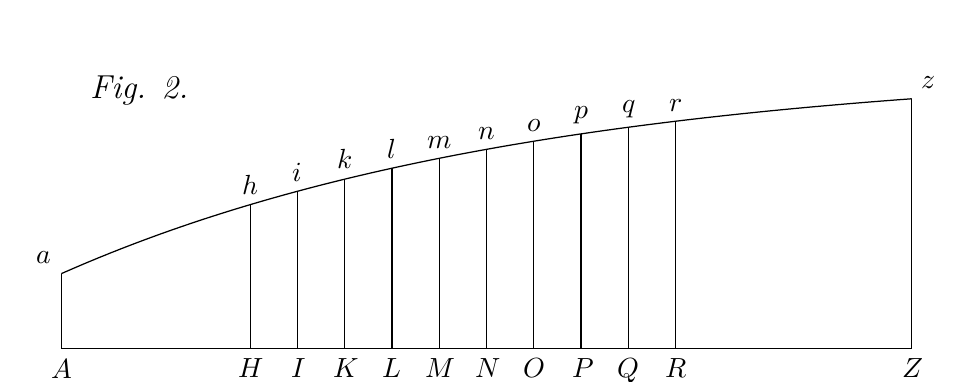
\begin{tikzpicture}[x=1.2cm,y=.95cm,line width=.45pt]
\draw (0,1)--(0,0)--(9,0)--(9,{1+2.8*(1-exp(-9/5))});
\draw[domain=0:9,samples=70] plot (\x,{1+2.8*(1-exp(-\x/5))});
\foreach \X/\U/\L in {2/H/h,2.5/I/i,3/K/k,3.5/L/l,4/M/m,4.5/N/n,5/O/o,5.5/P/p,6/Q/q,6.5/R/r}{
\draw (\X,0)--(\X,{1+2.8*(1-exp(-\X/5))});
\node[below] at (\X,0) {$\U$};
\node[above] at (\X,{1+2.8*(1-exp(-\X/5))}) {$\L$};}
\node[below] at (0,0) {$A$};\node[above left] at (0,1) {$a$};
\node[below] at (9,0) {$Z$};\node[above right] at (9,{1+2.8*(1-exp(-9/5))}) {$z$};
\node[anchor=west] at (.2,3.45) {\large\textit{Fig. 2.}};
\end{tikzpicture}
}\end{center}
\par\bigskip
\clearpage
\needspace{95mm}\hypertarget{fig:3}{}
\begin{center}\adjustbox{max width=\linewidth,max height=75mm}{% Modern editorial, markup and figure/layout contributions: CC-BY-SA-4.0.
% Historical text and illustrations: Leonhard Euler (1744), public domain.
% Component scope and upstream attribution: see RIGHTS.md.
% Vector redraw: Tabula I, Fig. 3. n and v are distinct points on one ordinate.
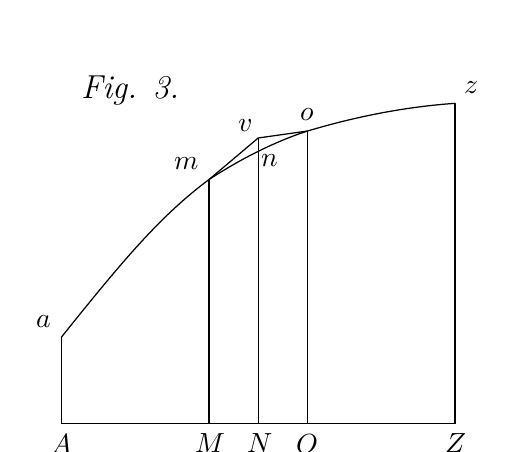
\begin{tikzpicture}[x=1.25cm,y=1.1cm,line width=.45pt]
\draw (0,1)--(0,0)--(4,0)--(4,3.7);
\draw (0,1) .. controls (.6,1.85) and (1,2.4) .. (1.5,2.82)
 .. controls (1.85,3.08) and (2.2,3.27) .. (2.5,3.38)
 .. controls (3,3.55) and (3.5,3.66) .. (4,3.7);
\draw (1.5,0)--(1.5,2.82) (2,0)--(2,3.30) (2.5,0)--(2.5,3.38);
\draw (1.5,2.82)--(2,3.30)--(2.5,3.38);
\foreach \x/\t in {0/A,1.5/M,2/N,2.5/O,4/Z}{\node[below] at (\x,0) {$\t$};}
\node[above left] at (0,1) {$a$};\node[above left] at (1.5,2.82) {$m$};
\node[below right,inner sep=1pt] at (2,3.15) {$n$};
\node[above left,inner sep=2pt] at (2,3.30) {$v$};
\node[above] at (2.5,3.38) {$o$};\node[above right] at (4,3.7) {$z$};
\node[anchor=west] at (.1,3.85) {\large\textit{Fig. 3.}};
\end{tikzpicture}
}\end{center}
\par\bigskip
\needspace{95mm}\hypertarget{fig:4}{}
\begin{center}\adjustbox{max width=\linewidth,max height=75mm}{% Modern editorial, markup and figure/layout contributions: CC-BY-SA-4.0.
% Historical text and illustrations: Leonhard Euler (1744), public domain.
% Component scope and upstream attribution: see RIGHTS.md.
% Tabula I Fig.4: incidence and labels retained, schematic coordinates.
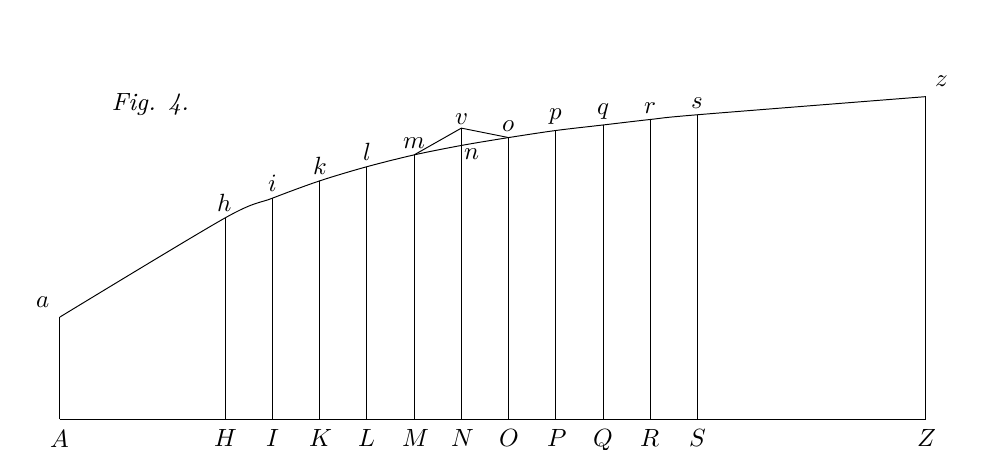
\begin{tikzpicture}[x=1cm,y=1cm,line width=.35pt,font=\small]
\draw (0,0)--(11,0)--(11,4.1);
\draw (0,0)--(0,1.3);
\draw plot[smooth] coordinates {(0,1.3) (2.1,2.56) (2.7,2.81) (3.3,3.03) (3.9,3.21) (4.5,3.36) (5.1,3.48) (5.7,3.58) (6.3,3.67) (6.9,3.74) (7.5,3.81) (8.1,3.87) (11,4.1)};
\node[below] at (0,0) {$A$};\node[above left] at (0,1.3) {$a$};
\node[below] at (11,0) {$Z$};\node[above right] at (11,4.1) {$z$};
\foreach \x/\y/\a/\b in {2.1/2.56/H/h,2.7/2.81/I/i,3.3/3.03/K/k,3.9/3.21/L/l,4.5/3.36/M/m,5.1/3.48/N/n,5.7/3.58/O/o,6.3/3.67/P/p,6.9/3.74/Q/q,7.5/3.81/R/r,8.1/3.87/S/s}{
 \draw (\x,0)--(\x,\y);\node[below] at (\x,0) {$\a$};
 \ifdim\x pt=5.1pt\node[below right,inner sep=1pt] at (\x,\y) {$\b$};\else\node[above,inner sep=2pt] at (\x,\y) {$\b$};\fi
}
\draw (4.5,3.36)--(5.1,3.70)--(5.7,3.58);
\draw (5.1,3.48)--(5.1,3.70);
\node[above,inner sep=1pt] at (5.1,3.70) {$v$};
\node at (1.15,4) {\textit{Fig. 4.}};
\end{tikzpicture}
}\end{center}
\par\bigskip
\clearpage
\needspace{95mm}\hypertarget{fig:5}{}
\begin{center}\adjustbox{max width=\linewidth,max height=75mm}{% Modern editorial, markup and figure/layout contributions: CC-BY-SA-4.0.
% Historical text and illustrations: Leonhard Euler (1744), public domain.
% Component scope and upstream attribution: see RIGHTS.md.
% Tabula I Fig.5; curve and evolute schematic, source letter case retained.
\begin{tikzpicture}[x=1cm,y=1cm,line width=.35pt,font=\small]
\coordinate (A) at (0,0);\coordinate (M) at (3.5,0);\coordinate (m) at (3.5,3.15);\coordinate (R) at (6.6,-3.9);
\draw (A)--(5.2,0);
\draw (M)--(m);
\draw (0,0) .. controls (0.08,1.25) and (1.45,2.15) .. (m);
\draw (m)--(3.85,3.32);
\draw (m)--(R)--(6.85,-4.47);
\draw (A) .. controls (3.0,-.08) and (5.3,-1.36) .. (R);
\node[below left] at (A) {$A$};\node[below] at (M) {$M$};
\node[above] at (m) {$m$};\node[right] at (R) {$R$};
\node at (1,3.1) {\textit{Fig. 5.}};
\end{tikzpicture}
}\end{center}
\par\bigskip
\needspace{95mm}\hypertarget{fig:6}{}
\begin{center}\adjustbox{max width=\linewidth,max height=75mm}{% Modern editorial, markup and figure/layout contributions: CC-BY-SA-4.0.
% Historical text and illustrations: Leonhard Euler (1744), public domain.
% Component scope and upstream attribution: see RIGHTS.md.
% Tabula I Fig.6; vertical abscissa, horizontal tangent at A.
\begin{tikzpicture}[x=1cm,y=1cm,line width=.35pt,font=\small]
\draw (0,1.65)--(0,-5.6);
\draw (0,0)--(2.8,0);
\draw (0,0) .. controls (1.3,0) and (2.1,-.8) .. (2.62,-2.15) .. controls (3.1,-3.4) and (3.4,-4.8) .. (3.55,-6.0);
\draw (0,-2.15)--(2.62,-2.15);
\node[left] at (0,1.65) {$C$};\node[left] at (0,0) {$A$};
\node[right] at (2.8,0) {$a$};\node[left] at (0,-2.15) {$P$};
\node[right] at (2.62,-2.15) {$M$};
\node at (1.5,1.05) {\textit{Fig. 6.}};
\end{tikzpicture}
}\end{center}
\par\bigskip
\clearpage
\needspace{95mm}\hypertarget{fig:7}{}
\begin{center}\adjustbox{max width=\linewidth,max height=75mm}{% Modern editorial, markup and figure/layout contributions: CC-BY-SA-4.0.
% Historical text and illustrations: Leonhard Euler (1744), public domain.
% Component scope and upstream attribution: see RIGHTS.md.
% Manual vector redraw from E65 Tabula I, Fig. 7.
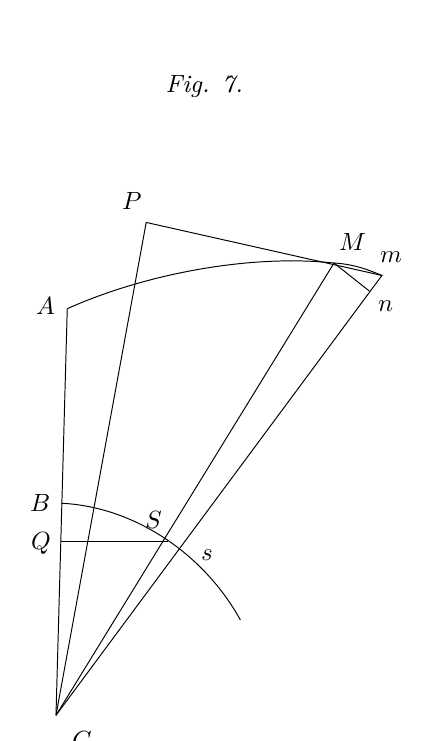
\begin{tikzpicture}[x=1cm,y=1cm,line width=.35pt,font=\small]
\draw (0.7664,0.3008)--(0.9096,5.4647);
\draw (0.7664,0.3008)--(1.9123,6.5605)--(4.9061,5.8873)--(0.7664,0.3008);
\draw (0.7664,0.3008)--(4.2973,6.0449);
\draw (4.2973,6.0449)--(4.7485,5.6868);
\draw (0.8308,2.5139)--(2.1916,2.5139);
\draw (0.9096,5.4647) .. controls (1.8980,5.9088) and (3.2373,6.1595) .. (4.2973,6.0449) .. controls (4.5623,6.0305) and (4.7485,5.9518) .. (4.9061,5.8873);
\draw (0.8380,2.9938) .. controls (1.7547,2.9508) and (2.6428,2.3564) .. (3.1084,1.5112);
\node[anchor=east,inner sep=1pt] at (0.8022,5.5005) {$A$};
\node[anchor=east,inner sep=1pt] at (0.7234,3.0009) {$B$};
\node[anchor=east,inner sep=1pt] at (0.7449,2.4853) {$Q$};
\node[anchor=north west,inner sep=1pt] at (0.9382,0.1432) {$C$};
\node[anchor=south east,inner sep=1pt] at (1.8550,6.6823) {$P$};
\node[anchor=south west,inner sep=1pt] at (4.3259,6.1595) {$M$};
\node[anchor=south west,inner sep=1pt] at (4.8488,6.0019) {$m$};
\node[anchor=north west,inner sep=1pt] at (4.8201,5.6080) {$n$};
\node[anchor=south east,inner sep=1pt] at (2.1415,2.6285) {$S$};
\node[anchor=west,inner sep=1pt] at (2.5784,2.3349) {$s$};
\node[anchor=south] at (2.6500,8.0216) {\textit{Fig. 7.}};
\end{tikzpicture}
}\end{center}
\par\bigskip
\needspace{95mm}\hypertarget{fig:8}{}
\begin{center}\adjustbox{max width=\linewidth,max height=75mm}{% Modern editorial, markup and figure/layout contributions: CC-BY-SA-4.0.
% Historical text and illustrations: Leonhard Euler (1744), public domain.
% Component scope and upstream attribution: see RIGHTS.md.
% Manual vector redraw from E65 Tabula I, Fig. 8.
\begin{tikzpicture}[x=1cm,y=1cm,line width=.35pt,font=\small]
\draw (0.9291,0.5946)--(5.0169,0.5946);
\draw (4.4223,0.5946)--(4.4743,4.4669);
\draw (0.9291,0.5946) .. controls (0.8770,2.3412) and (2.2149,4.2514) .. (4.9500,4.4818);
\node[anchor=north east,inner sep=1pt] at (0.8993,0.4757) {$A$};
\node[anchor=east,inner sep=1pt] at (0.8027,1.4716) {$B$};
\node[anchor=north,inner sep=1pt] at (4.4223,0.4757) {$P$};
\node[anchor=north,inner sep=1pt] at (5.0169,0.4757) {$C$};
\node[anchor=south,inner sep=1pt] at (4.4818,4.5412) {$M$};
\node[anchor=south] at (2.7500,5.2027) {\textit{Fig. 8.}};
\end{tikzpicture}
}\end{center}
\par\bigskip
\clearpage
\needspace{95mm}\hypertarget{fig:9}{}
\begin{center}\adjustbox{max width=\linewidth,max height=75mm}{% Modern editorial, markup and figure/layout contributions: CC-BY-SA-4.0.
% Historical text and illustrations: Leonhard Euler (1744), public domain.
% Component scope and upstream attribution: see RIGHTS.md.
% Manual vector redraw from E65 Tabula I, Fig. 9.
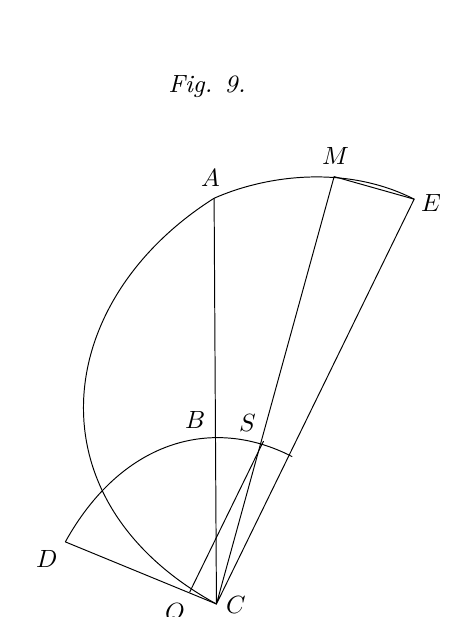
\begin{tikzpicture}[x=1cm,y=1cm,line width=.35pt,font=\small]
\draw (2.8696,0.3886)--(2.8397,5.5418);
\draw (2.8696,0.3886)--(4.3641,5.8168)--(5.3804,5.5299)--(2.8696,0.3886)--(0.9505,1.1777);
\draw (2.5288,0.5380)--(3.4674,2.4571);
\draw (2.8696,0.3886) .. controls (0.4783,1.6978) and (0.7712,4.2326) .. (2.8397,5.5418) .. controls (3.5451,5.8527) and (4.5495,5.9543) .. (5.3804,5.5299);
\draw (0.9505,1.1777) .. controls (1.6500,2.4391) and (2.7918,2.7978) .. (3.8321,2.2598);
\node[anchor=south,inner sep=1pt] at (2.8038,5.6435) {$A$};
\node[anchor=south,inner sep=1pt] at (4.3641,5.9245) {$M$};
\node[anchor=west,inner sep=1pt] at (5.4283,5.4821) {$E$};
\node[anchor=south east,inner sep=1pt] at (2.7620,2.5826) {$B$};
\node[anchor=south east,inner sep=1pt] at (3.4016,2.5348) {$S$};
\node[anchor=north east,inner sep=1pt] at (0.8908,1.1120) {$D$};
\node[anchor=north east,inner sep=1pt] at (2.5109,0.4484) {$Q$};
\node[anchor=west,inner sep=1pt] at (2.9592,0.3707) {$C$};
\node[anchor=south] at (2.7500,6.6957) {\textit{Fig. 9.}};
\end{tikzpicture}
}\end{center}
\par\bigskip
\needspace{95mm}\hypertarget{fig:10}{}
\begin{center}\adjustbox{max width=\linewidth,max height=75mm}{% Modern editorial, markup and figure/layout contributions: CC-BY-SA-4.0.
% Historical text and illustrations: Leonhard Euler (1744), public domain.
% Component scope and upstream attribution: see RIGHTS.md.
% Manual vector redraw from E65 Tabula I, Fig. 10.
\begin{tikzpicture}[x=1cm,y=1cm,line width=.35pt,font=\small]
\draw (0.2989,0.9489)--(5.4167,0.9489);
\draw (2.6971,0.9489)--(2.6971,2.8466)--(4.6920,4.7592);
\draw (0.2989,0.9489) .. controls (0.3661,2.1144) and (2.7345,3.1006) .. (6.1264,3.7356);
\node[anchor=north,inner sep=1pt] at (0.2839,0.8443) {$A$};
\node[anchor=north,inner sep=1pt] at (2.6971,0.8443) {$P$};
\node[anchor=south east,inner sep=1pt] at (2.6000,2.9437) {$Q$};
\node[anchor=south,inner sep=1pt] at (4.6920,4.8414) {$M$};
\node[anchor=south] at (3.2500,5.4540) {\textit{Fig. 10.}};
\end{tikzpicture}
}\end{center}
\par\bigskip
\clearpage
\needspace{95mm}\hypertarget{fig:11}{}
\begin{center}\adjustbox{max width=\linewidth,max height=75mm}{% Modern editorial, markup and figure/layout contributions: CC-BY-SA-4.0.
% Historical text and illustrations: Leonhard Euler (1744), public domain.
% Component scope and upstream attribution: see RIGHTS.md.
% Manual vector redraw from E65 Tabula II, Fig. 11.
\begin{tikzpicture}[x=1cm,y=1cm,line width=.35pt,font=\small]
\draw (0.2866,1.2806)--(5.5522,1.2806);
\draw (2.6418,1.2806)--(2.6418,3.7970)--(3.9761,1.2806);
\draw (0.2866,1.2806) .. controls (0.3134,2.8209) and (1.9701,3.7164) .. (5.3642,4.8896);
\node[anchor=north,inner sep=1pt] at (0.2687,1.1642) {$A$};
\node[anchor=north,inner sep=1pt] at (2.6418,1.1642) {$P$};
\node[anchor=north,inner sep=1pt] at (3.9761,1.1642) {$N$};
\node[anchor=south east,inner sep=1pt] at (2.5254,3.9045) {$M$};
\node[anchor=south] at (3.0000,5.4627) {\textit{Fig. 11.}};
\end{tikzpicture}
}\end{center}
\par\bigskip
\needspace{95mm}\hypertarget{fig:12}{}
\begin{center}\adjustbox{max width=\linewidth,max height=75mm}{% Modern editorial, markup and figure/layout contributions: CC-BY-SA-4.0.
% Historical text and illustrations: Leonhard Euler (1744), public domain.
% Component scope and upstream attribution: see RIGHTS.md.
% Manual vector redraw from E65 Tabula II, Fig. 12.
\begin{tikzpicture}[x=1cm,y=1cm,line width=.35pt,font=\small]
\draw (0.8118,3.0265)--(0.8118,0.2647)--(5.4176,0.2647);
\draw (2.1176,4.0235)--(2.1706,0.2647);
\draw (0.8118,3.0265)--(3.0441,1.5353)--(2.1176,4.0235);
\draw (0.4324,0.9706) .. controls (0.1059,2.9912) and (1.5706,4.4735) .. (3.4500,4.1471) .. controls (5.2147,3.8206) and (6.2559,2.2588) .. (5.4176,0.2647);
\node[anchor=north,inner sep=1pt] at (0.8118,0.1324) {$A$};
\node[anchor=north,inner sep=1pt] at (2.1706,0.1324) {$P$};
\node[anchor=north west,inner sep=1pt] at (5.4529,0.2029) {$D$};
\node[anchor=south east,inner sep=1pt] at (0.7059,3.0971) {$B$};
\node[anchor=south east,inner sep=1pt] at (2.0118,4.1382) {$M$};
\node[anchor=west,inner sep=1pt] at (3.1500,1.4912) {$C$};
\node[anchor=south] at (3.0000,5.3824) {\textit{Fig. 12.}};
\end{tikzpicture}
}\end{center}
\par\bigskip
\clearpage
\needspace{95mm}\hypertarget{fig:13}{}
\begin{center}\adjustbox{max width=\linewidth,max height=75mm}{% Modern editorial, markup and figure/layout contributions: CC-BY-SA-4.0.
% Historical text and illustrations: Leonhard Euler (1744), public domain.
% Component scope and upstream attribution: see RIGHTS.md.
% Manual vector redraw from E65 Tabula II, Fig. 13.
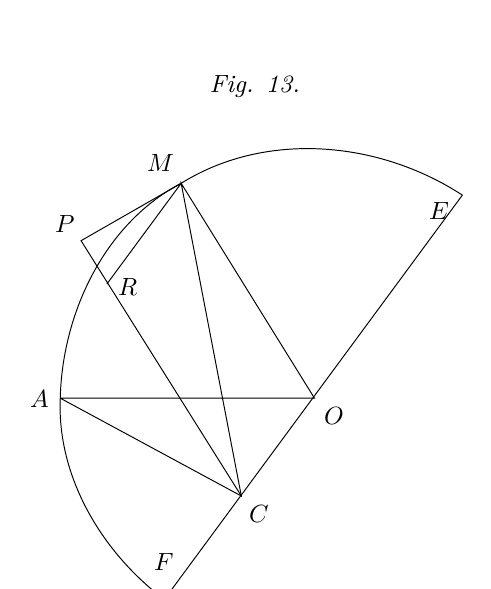
\begin{tikzpicture}[x=1cm,y=1cm,line width=.35pt,font=\small]
\draw (0.5286,2.7357)--(3.7571,2.7357)--(2.0643,5.4643)--(2.8286,1.4929)--(0.5286,2.7357);
\draw (1.8500,0.1786)--(5.6357,5.3143);
\draw (2.8286,1.4929)--(0.7929,4.7357)--(2.0643,5.4643)--(1.1214,4.1857);
\draw (1.8500,0.1786) .. controls (1.0571,0.7786) and (0.4857,1.7357) .. (0.5286,2.7357) .. controls (0.5571,3.8643) and (1.1286,4.9786) .. (2.0643,5.4643) .. controls (3.1143,6.1214) and (4.5500,6.0214) .. (5.6357,5.3143);
\node[anchor=east,inner sep=1pt] at (0.4286,2.7357) {$A$};
\node[anchor=south east,inner sep=1pt] at (1.9857,5.5714) {$M$};
\node[anchor=north east,inner sep=1pt] at (5.4929,5.2643) {$E$};
\node[anchor=north west,inner sep=1pt] at (3.8429,2.6643) {$O$};
\node[anchor=north west,inner sep=1pt] at (2.8929,1.4214) {$C$};
\node[anchor=south east,inner sep=1pt] at (1.9714,0.5000) {$F$};
\node[anchor=south east,inner sep=1pt] at (0.7143,4.7929) {$P$};
\node[anchor=west,inner sep=1pt] at (1.2286,4.1429) {$R$};
\node[anchor=south] at (3.0000,6.4286) {\textit{Fig. 13.}};
\end{tikzpicture}
}\end{center}
\par\bigskip
\needspace{95mm}\hypertarget{fig:14}{}
\begin{center}\adjustbox{max width=\linewidth,max height=75mm}{% Modern editorial, markup and figure/layout contributions: CC-BY-SA-4.0.
% Historical text and illustrations: Leonhard Euler (1744), public domain.
% Component scope and upstream attribution: see RIGHTS.md.
% Manual vector redraw from E65 Tabula II, Fig. 14.
\begin{tikzpicture}[x=1cm,y=1cm,line width=.35pt,font=\small]
\draw (0.2809,4.2531)--(6.3636,4.2531);
\draw (3.5068,4.2531)--(3.4426,0.5858);
\draw (1.1074,2.6883)--(5.7056,2.6883);
\draw (0.2809,4.2531) .. controls (1.2599,1.9259) and (2.1105,0.5778) .. (3.4426,0.5858) .. controls (4.7907,0.5858) and (5.7617,2.4877) .. (6.3636,4.2531);
\node[anchor=south,inner sep=1pt] at (0.2809,4.3574) {$D$};
\node[anchor=south,inner sep=1pt] at (6.3636,4.3574) {$D$};
\node[anchor=east,inner sep=1pt] at (1.0111,2.6562) {$M$};
\node[anchor=west,inner sep=1pt] at (5.8019,2.6562) {$M$};
\node[anchor=north west,inner sep=1pt] at (3.5710,4.1247) {$C$};
\node[anchor=south west,inner sep=1pt] at (3.5710,2.7525) {$P$};
\node[anchor=west,inner sep=1pt] at (3.5870,2.2630) {$G$};
\node[anchor=north,inner sep=1pt] at (3.4426,0.4815) {$A$};
\node[anchor=south] at (3.2500,5.1358) {\textit{Fig. 14.}};
\end{tikzpicture}
}\end{center}
\par\bigskip
\clearpage
\needspace{95mm}\hypertarget{fig:15}{}
\begin{center}\adjustbox{max width=\linewidth,max height=75mm}{% Modern editorial, markup and figure/layout contributions: CC-BY-SA-4.0.
% Historical text and illustrations: Leonhard Euler (1744), public domain.
% Component scope and upstream attribution: see RIGHTS.md.
% Manual vector redraw from E65 Tabula II, Fig. 15.
\begin{tikzpicture}[x=1cm,y=1cm,line width=.35pt,font=\small]
\draw (0.3630,1.2444)--(0.3630,0.5185)--(11.5407,0.5185)--(11.5407,5.9630);
\draw (0.3630,1.2444) .. controls (3.3556,1.8741) and (6.0593,2.5556) .. (7.9259,3.2889) .. controls (9.6370,3.9704) and (10.9185,5.0148) .. (11.5407,5.9630);
\draw (3.2222,0.5185)--(3.2222,1.8889);
\node[anchor=north,inner sep=1pt] at (3.2222,0.4148) {$I$};
\node[anchor=south,inner sep=1pt] at (3.2222,1.9778) {$i$};
\draw (3.6889,0.5185)--(3.6889,2.0000);
\node[anchor=north,inner sep=1pt] at (3.6889,0.4148) {$K$};
\node[anchor=south,inner sep=1pt] at (3.6889,2.0889) {$k$};
\draw (4.1926,0.5185)--(4.1926,2.1333);
\node[anchor=north,inner sep=1pt] at (4.1926,0.4148) {$L$};
\node[anchor=south,inner sep=1pt] at (4.1926,2.2222) {$l$};
\draw (4.6148,0.5185)--(4.6148,2.2370);
\node[anchor=north,inner sep=1pt] at (4.6148,0.4148) {$M$};
\node[anchor=south,inner sep=1pt] at (4.6148,2.3259) {$m$};
\draw (5.0741,0.5185)--(5.0741,2.3556);
\node[anchor=north,inner sep=1pt] at (5.0741,0.4148) {$N$};
\draw (5.5185,0.5185)--(5.5185,2.4815);
\node[anchor=north,inner sep=1pt] at (5.5185,0.4148) {$O$};
\draw (6.0000,0.5185)--(6.0000,2.6296);
\node[anchor=north,inner sep=1pt] at (6.0000,0.4148) {$P$};
\node[anchor=south,inner sep=1pt] at (6.0000,2.7185) {$p$};
\draw (6.4815,0.5185)--(6.4815,2.8148);
\node[anchor=north,inner sep=1pt] at (6.4815,0.4148) {$Q$};
\node[anchor=south,inner sep=1pt] at (6.4815,2.9037) {$q$};
\draw (6.9333,0.5185)--(6.9333,2.9481);
\node[anchor=north,inner sep=1pt] at (6.9333,0.4148) {$R$};
\node[anchor=south,inner sep=1pt] at (6.9333,3.0370) {$r$};
\draw (7.3778,0.5185)--(7.3778,3.1259);
\node[anchor=north,inner sep=1pt] at (7.3778,0.4148) {$S$};
\node[anchor=south,inner sep=1pt] at (7.3778,3.2148) {$s$};
\draw (7.8741,0.5185)--(7.8741,3.2889);
\node[anchor=north,inner sep=1pt] at (7.8741,0.4148) {$T$};
\node[anchor=south,inner sep=1pt] at (7.8741,3.3778) {$t$};
\draw (4.6148,2.2370)--(5.0741,2.4963)--(5.5185,2.6148)--(6.0000,2.6296);
\draw (5.0741,2.3556)--(5.0741,2.4963);
\draw (5.5185,2.4815)--(5.5185,2.6148);
\node[anchor=north west,inner sep=1pt] at (5.1185,2.2296) {$n$};
\node[anchor=north west,inner sep=1pt] at (5.5556,2.3852) {$o$};
\node[anchor=south,inner sep=1pt] at (5.0148,2.5926) {$v$};
\node[anchor=south,inner sep=1pt] at (5.5185,2.7111) {$\omega$};
\node[anchor=north,inner sep=1pt] at (0.3630,0.4222) {$A$};
\node[anchor=south,inner sep=1pt] at (0.3259,1.3630) {$a$};
\node[anchor=north,inner sep=1pt] at (11.5407,0.4222) {$Z$};
\node[anchor=south,inner sep=1pt] at (11.5407,6.0519) {$z$};
\node[anchor=south] at (6.0000,6.1481) {\textit{Fig. 15.}};
\end{tikzpicture}
}\end{center}
\par\bigskip
\needspace{95mm}\hypertarget{fig:16}{}
\begin{center}\adjustbox{max width=\linewidth,max height=75mm}{% Modern editorial, markup and figure/layout contributions: CC-BY-SA-4.0.
% Historical text and illustrations: Leonhard Euler (1744), public domain.
% Component scope and upstream attribution: see RIGHTS.md.
% Manual vector redraw from E65 Tabula II, Fig. 16.
\begin{tikzpicture}[x=1cm,y=1cm,line width=.35pt,font=\small]
\draw (0.5037,3.7732)--(0.5463,1.6220)--(6.7610,1.6220)--(6.7695,4.8402);
\draw (0.5037,3.7732) .. controls (2.3988,4.9427) and (4.3110,5.2756) .. (6.7695,4.8402);
\draw (0.5037,3.7732) .. controls (0.7171,2.9110) and (1.0841,2.0744) .. (1.4171,1.6220) .. controls (1.9293,0.8110) and (2.5354,0.3500) .. (3.3207,0.3500) .. controls (4.1061,0.3500) and (4.8146,0.9817) .. (5.3183,1.6220) .. controls (6.0695,2.5524) and (6.5732,3.6707) .. (6.7695,4.8402);
\node[anchor=south east,inner sep=1pt] at (0.3927,3.8585) {$a$};
\node[anchor=south west,inner sep=1pt] at (6.8549,4.8659) {$z$};
\node[anchor=north,inner sep=1pt] at (0.5207,1.5024) {$A$};
\node[anchor=south east,inner sep=1pt] at (6.6415,1.7159) {$Z$};
\node[anchor=south west,inner sep=1pt] at (1.4171,1.7073) {$C$};
\node[anchor=south east,inner sep=1pt] at (5.3183,1.7329) {$D$};
\node[anchor=south,inner sep=1pt] at (3.3207,0.4439) {$E$};
\node[anchor=south] at (3.5000,5.5488) {\textit{Fig. 16.}};
\end{tikzpicture}
}\end{center}
\par\bigskip
\clearpage
\needspace{95mm}\hypertarget{fig:17}{}
\begin{center}\adjustbox{max width=\linewidth,max height=75mm}{% Modern editorial, markup and figure/layout contributions: CC-BY-SA-4.0.
% Historical text and illustrations: Leonhard Euler (1744), public domain.
% Component scope and upstream attribution: see RIGHTS.md.
% Manual vector redraw from E65 Tabula II, Fig. 17.
\begin{tikzpicture}[x=1cm,y=1cm,line width=.35pt,font=\small]
\draw (0.0867,0.6933)--(6.2313,0.6933)--(6.2573,3.9520);
\draw (3.9347,0.6933)--(3.9347,2.2273);
\draw (0.0867,0.6933) .. controls (2.4007,1.1440) and (4.5673,2.2187) .. (6.2573,3.9520);
\node[anchor=north,inner sep=1pt] at (0.2080,0.5633) {$A$};
\node[anchor=north,inner sep=1pt] at (3.9347,0.5633) {$P$};
\node[anchor=west,inner sep=1pt] at (6.3613,0.6500) {$B$};
\node[anchor=west,inner sep=1pt] at (6.3700,3.9433) {$C$};
\node[anchor=south east,inner sep=1pt] at (3.8480,2.3313) {$M$};
\node[anchor=south] at (3.2500,4.5933) {\textit{Fig. 17.}};
\end{tikzpicture}
}\end{center}
\par\bigskip
\needspace{95mm}\hypertarget{fig:18}{}
\begin{center}\adjustbox{max width=\linewidth,max height=75mm}{% Modern editorial, markup and figure/layout contributions: CC-BY-SA-4.0.
% Historical text and illustrations: Leonhard Euler (1744), public domain.
% Component scope and upstream attribution: see RIGHTS.md.
% Manual vector redraw from E65 Tabula II, Fig. 18.
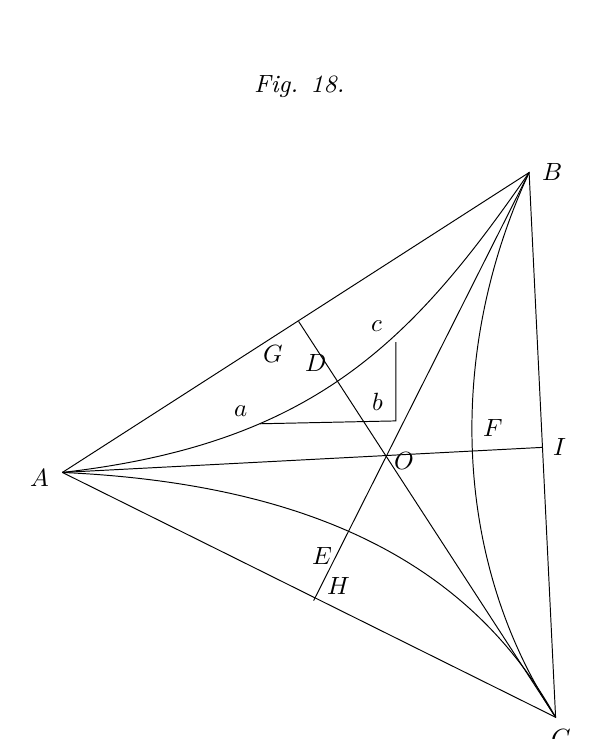
\begin{tikzpicture}[x=1cm,y=1cm,line width=.35pt,font=\small]
\draw (0.4909,3.5455)--(6.4182,7.3545)--(6.7545,0.4364)--(0.4909,3.5455);
\draw (0.4909,3.5455)--(6.5818,3.8636);
\draw (3.4909,5.4636)--(6.7545,0.4364);
\draw (3.6818,1.9182)--(6.4182,7.3545);
\draw (0.4909,3.5455) .. controls (3.6636,3.9091) and (4.9182,5.1818) .. (6.4182,7.3545);
\draw (0.4909,3.5455) .. controls (3.7182,3.4000) and (5.6909,2.3455) .. (6.7545,0.4364);
\draw (6.4182,7.3545) .. controls (5.3455,5.0364) and (5.4636,2.3818) .. (6.7545,0.4364);
\draw (3.0000,4.1636)--(4.7273,4.2000)--(4.7273,5.2000);
\node[anchor=east,inner sep=1pt] at (0.3636,3.4818) {$A$};
\node[anchor=west,inner sep=1pt] at (6.5455,7.3636) {$B$};
\node[anchor=north,inner sep=1pt] at (6.8182,0.3273) {$C$};
\node[anchor=west,inner sep=1pt] at (6.6818,3.8636) {$I$};
\node[anchor=west,inner sep=1pt] at (4.6727,3.6909) {$O$};
\node[anchor=south west,inner sep=1pt] at (5.8000,3.9636) {$F$};
\node[anchor=north east,inner sep=1pt] at (3.3364,5.2091) {$G$};
\node[anchor=south east,inner sep=1pt] at (3.8818,4.7818) {$D$};
\node[anchor=north east,inner sep=1pt] at (3.9364,2.6364) {$E$};
\node[anchor=west,inner sep=1pt] at (3.8182,2.1000) {$H$};
\node[anchor=south,inner sep=1pt] at (2.7545,4.2091) {$a$};
\node[anchor=south east,inner sep=1pt] at (4.6091,4.2818) {$b$};
\node[anchor=south east,inner sep=1pt] at (4.6000,5.2909) {$c$};
\node[anchor=south] at (3.5000,8.1818) {\textit{Fig. 18.}};
\end{tikzpicture}
}\end{center}
\par\bigskip
\clearpage
\needspace{95mm}\hypertarget{fig:19}{}
\begin{center}\adjustbox{max width=\linewidth,max height=75mm}{% Modern editorial, markup and figure/layout contributions: CC-BY-SA-4.0.
% Historical text and illustrations: Leonhard Euler (1744), public domain.
% Component scope and upstream attribution: see RIGHTS.md.
% Manual vector redraw from E65 Tabula II, Fig. 19.
\begin{tikzpicture}[x=1cm,y=1cm,line width=.35pt,font=\small]
\draw (0.2333,2.2304)--(6.3480,2.2578);
\draw (2.2647,5.8608)--(2.3333,1.4275)--(6.9108,1.4343)--(2.2647,5.8608);
\draw (0.2333,2.2304) .. controls (0.2539,3.5755) and (1.4137,5.1745) .. (2.6627,6.1627);
\draw (0.2333,2.2304) .. controls (1.6814,1.9559) and (3.3216,1.1324) .. (4.2961,0.0069);
\node[anchor=north,inner sep=1pt] at (0.2333,2.1206) {$A$};
\node[anchor=south east,inner sep=1pt] at (2.1824,5.9500) {$M$};
\node[anchor=south west,inner sep=1pt] at (2.4020,2.3471) {$P$};
\node[anchor=north east,inner sep=1pt] at (2.2441,1.3382) {$N$};
\node[anchor=north,inner sep=1pt] at (6.9039,1.3382) {$O$};
\node[anchor=south] at (3.5000,6.4510) {\textit{Fig. 19.}};
\end{tikzpicture}
}\end{center}
\par\bigskip
\needspace{95mm}\hypertarget{fig:20}{}
\begin{center}\adjustbox{max width=\linewidth,max height=75mm}{% Modern editorial, markup and figure/layout contributions: CC-BY-SA-4.0.
% Historical text and illustrations: Leonhard Euler (1744), public domain.
% Component scope and upstream attribution: see RIGHTS.md.
% Manual vector redraw from E65 Tabula II, Fig. 20.
\begin{tikzpicture}[x=1cm,y=1cm,line width=.35pt,font=\small]
\draw (0.3318,2.9341)--(0.3318,0.0175)--(5.4752,0.0175)--(5.4141,4.4797);
\draw (0.3318,2.9341)--(5.4403,2.9341);
\draw (2.8118,0.0175)--(2.7944,2.9341);
\draw (0.3318,2.0783) .. controls (1.9211,2.0783) and (4.1392,3.0476) .. (5.4141,4.4797);
\node[anchor=north,inner sep=1pt] at (0.3318,-0.1135) {$A$};
\node[anchor=north,inner sep=1pt] at (5.4752,-0.1135) {$B$};
\node[anchor=north,inner sep=1pt] at (2.8118,-0.1135) {$P$};
\node[anchor=east,inner sep=1pt] at (0.2270,2.0783) {$a$};
\node[anchor=south west,inner sep=1pt] at (5.5101,4.5408) {$b$};
\node[anchor=east,inner sep=1pt] at (0.2270,2.9341) {$\alpha$};
\node[anchor=west,inner sep=1pt] at (5.5451,2.9341) {$\beta$};
\node[anchor=south,inner sep=1pt] at (2.7420,3.0476) {$m$};
\node[anchor=north west,inner sep=1pt] at (2.9166,2.6634) {$M$};
\node[anchor=south] at (3.1000,4.8901) {\textit{Fig. 20.}};
\end{tikzpicture}
}\end{center}
\par\bigskip
\clearpage
\needspace{95mm}\hypertarget{fig:21}{}
\begin{center}\adjustbox{max width=\linewidth,max height=75mm}{% Modern editorial, markup and figure/layout contributions: CC-BY-SA-4.0.
% Historical text and illustrations: Leonhard Euler (1744), public domain.
% Component scope and upstream attribution: see RIGHTS.md.
% Manual vector redraw from E65 Tabula II, Fig. 21.
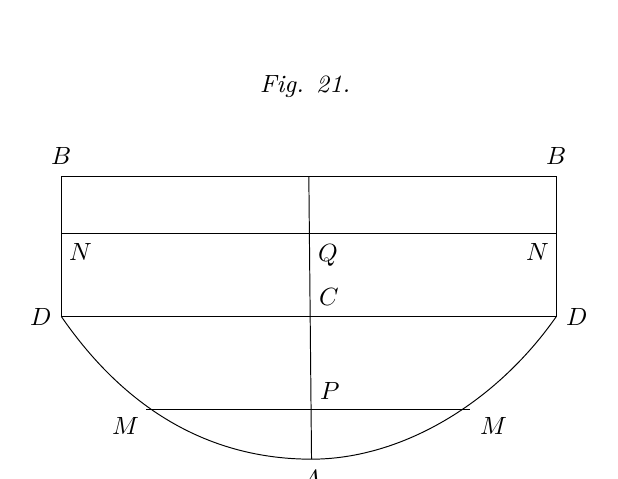
\begin{tikzpicture}[x=1cm,y=1cm,line width=.35pt,font=\small]
\draw (0.4049,4.2755)--(6.6912,4.2755)--(6.6912,2.4912)--(0.4049,2.4912)--(0.4049,4.2755);
\draw (0.4049,3.5412)--(6.6912,3.5412);
\draw (3.5480,4.2755)--(3.5824,0.6794);
\draw (1.4824,1.3108)--(5.5931,1.3108);
\draw (0.4049,2.4912) .. controls (1.2559,1.2559) and (2.3471,0.6794) .. (3.5824,0.6794) .. controls (4.7353,0.6794) and (5.9294,1.4000) .. (6.6912,2.4912);
\node[anchor=south,inner sep=1pt] at (0.4049,4.3853) {$B$};
\node[anchor=south,inner sep=1pt] at (6.6912,4.3853) {$B$};
\node[anchor=north west,inner sep=1pt] at (0.4735,3.4588) {$N$};
\node[anchor=north east,inner sep=1pt] at (6.6088,3.4588) {$N$};
\node[anchor=north west,inner sep=1pt] at (3.6304,3.4520) {$Q$};
\node[anchor=east,inner sep=1pt] at (0.3157,2.4912) {$D$};
\node[anchor=west,inner sep=1pt] at (6.7804,2.4912) {$D$};
\node[anchor=south west,inner sep=1pt] at (3.6441,2.5804) {$C$};
\node[anchor=south west,inner sep=1pt] at (3.6510,1.3931) {$P$};
\node[anchor=north east,inner sep=1pt] at (1.4069,1.2490) {$M$};
\node[anchor=north west,inner sep=1pt] at (5.6824,1.2490) {$M$};
\node[anchor=north,inner sep=1pt] at (3.5824,0.5902) {$A$};
\node[anchor=south] at (3.5000,5.1471) {\textit{Fig. 21.}};
\end{tikzpicture}
}\end{center}
\par\bigskip

\bookpart{addfigures}{Figuræ ad additamenta I–II}{Figuræ additamentorum}
\section*{Figuræ ad additamenta I–II}
\noindent\textit{Ex Tabulis III, IV et V. Numeri proprii additamentorum.}\par\bigskip
\needspace{95mm}\hypertarget{addfig:1}{}
\begin{center}\adjustbox{max width=\linewidth,max height=75mm}{% Modern editorial, markup and figure/layout contributions: CC-BY-SA-4.0.
% Historical text and illustrations: Leonhard Euler (1744), public domain.
% Component scope and upstream attribution: see RIGHTS.md.
% Manual vector redrawing after E65, Tabula III. Schematic coordinates; original point relations retained.
\begin{tikzpicture}[x=1cm,y=1cm,line width=.35pt,font=\small]
\draw (0,0)..controls (.1,1.4) and (1.5,2.6)..(2.6,3.2)..controls (3.2,3.5) and (4.1,3.85)..(5,4.2);
\draw (2.6,3.2)--(5.3,-1.8);
\node[below,inner sep=2pt] at (0,0) {$A$};
\node[above left,inner sep=2pt] at (2.6,3.2) {$M$};
\node[above,inner sep=2pt] at (3.15,3.47) {$m$};
\node[right,inner sep=2pt] at (5,4.2) {$B$};
\node[below,inner sep=2pt] at (5.3,-1.8) {$R$};
\node[anchor=north] at ([yshift=-4mm]current bounding box.south) {\textit{Fig. 1.}};
\end{tikzpicture}
}\end{center}
\par\bigskip
\needspace{95mm}\hypertarget{addfig:2}{}
\begin{center}\adjustbox{max width=\linewidth,max height=75mm}{% Modern editorial, markup and figure/layout contributions: CC-BY-SA-4.0.
% Historical text and illustrations: Leonhard Euler (1744), public domain.
% Component scope and upstream attribution: see RIGHTS.md.
% Manual vector redrawing after E65, Tabula III. Schematic coordinates; original point relations retained.
\begin{tikzpicture}[x=1cm,y=1cm,line width=.35pt,font=\small]
\draw (0,0)..controls (.12,1.25) and (1.15,1.8)..(2.5,2.3)..controls (4.1,2.9) and (5.3,3.5)..(6,4.5);
\draw (0,0)--(5.8,0) (2.5,0)--(2.5,2.3);
\node[below,inner sep=2pt] at (0,0) {$A$};
\node[above left,inner sep=2pt] at (2.5,2.3) {$M$};
\node[above,inner sep=2pt] at (3.1,2.54) {$m$};
\node[right,inner sep=2pt] at (6,4.5) {$B$};
\node[below,inner sep=2pt] at (2.5,0) {$P$};
\node[below,inner sep=2pt] at (5.8,0) {$D$};
\node[anchor=north] at ([yshift=-4mm]current bounding box.south) {\textit{Fig. 2.}};
\end{tikzpicture}
}\end{center}
\par\bigskip
\clearpage
\needspace{95mm}\hypertarget{addfig:3}{}
\begin{center}\adjustbox{max width=\linewidth,max height=75mm}{% Modern editorial, markup and figure/layout contributions: CC-BY-SA-4.0.
% Historical text and illustrations: Leonhard Euler (1744), public domain.
% Component scope and upstream attribution: see RIGHTS.md.
% Manual vector redrawing after E65, Tabula III. Schematic coordinates; original point relations retained.
\begin{tikzpicture}[x=1cm,y=1cm,line width=.35pt,font=\small]
\draw (-1,0)--(5.7,0) (.5,0)--(5.55,3.45) (1.2,-1.9)--(1.2,.48)--(2.85,-1.6) (3.65,0)--(3.65,2.15);
\draw (1.9,0)..controls (2.05,1.05) and (2.85,1.6)..(3.65,2.15);
\draw (5.3,3.8)--(4.9,3.57)--(5.28,2.97)--(5.7,3.2);
\draw (1.2,-2.12) circle (.22);
\node[below,inner sep=2pt] at (0.5,0) {$T$};
\node[below left,inner sep=2pt] at (1.2,0) {$C$};
\node[above right,inner sep=2pt] at (1.9,0) {$A$};
\node[below,inner sep=2pt] at (3.65,0) {$P$};
\node[above left,inner sep=2pt] at (3.65,2.15) {$M$};
\node[right,inner sep=2pt] at (5.55,3.45) {$B$};
\node[above left,inner sep=2pt] at (1.2,0.48) {$N$};
\node[right,inner sep=2pt] at (1.2,-1.9) {$D$};
\node[below,inner sep=2pt] at (2.85,-1.6) {$Q$};
\node[anchor=north] at ([yshift=-4mm]current bounding box.south) {\textit{Fig. 3.}};
\end{tikzpicture}
}\end{center}
\par\bigskip
\needspace{95mm}\hypertarget{addfig:4}{}
\begin{center}\adjustbox{max width=\linewidth,max height=75mm}{% Modern editorial, markup and figure/layout contributions: CC-BY-SA-4.0.
% Historical text and illustrations: Leonhard Euler (1744), public domain.
% Component scope and upstream attribution: see RIGHTS.md.
% Manual vector redrawing after E65, Tabula III. Schematic coordinates; original point relations retained.
\begin{tikzpicture}[x=1cm,y=1cm,line width=.35pt,font=\small]
\draw (0,-3.1)--(0,3.5) (0,1)--(4.3,1) (0,2)--(3.4,3) (3.4,1)--(3.4,3);
\draw (0,-2)..controls (.65,-.55) and (.95,.6)..(1.2,1)..controls (1.7,2.03) and (2.7,2.85)..(3.4,3)..controls (3.7,3.07) and (4,3.1)..(4.2,3.1);
\node[left,inner sep=2pt] at (0,3.5) {$R$};
\node[left,inner sep=2pt] at (0,2) {$N$};
\node[left,inner sep=2pt] at (0,1) {$C$};
\node[left,inner sep=2pt] at (0,-2) {$D$};
\node[left,inner sep=2pt] at (0,-3.1) {$E$};
\node[below right,inner sep=2pt] at (1.2,1) {$A$};
\node[above,inner sep=2pt] at (3.4,3) {$M$};
\node[below,inner sep=2pt] at (3.4,1) {$P$};
\node[anchor=north] at ([yshift=-4mm]current bounding box.south) {\textit{Fig. 4.}};
\end{tikzpicture}
}\end{center}
\par\bigskip
\clearpage
\needspace{95mm}\hypertarget{addfig:5}{}
\begin{center}\adjustbox{max width=\linewidth,max height=75mm}{% Modern editorial, markup and figure/layout contributions: CC-BY-SA-4.0.
% Historical text and illustrations: Leonhard Euler (1744), public domain.
% Component scope and upstream attribution: see RIGHTS.md.
% Manual vector redrawing after E65, Tabula III. Schematic coordinates; original point relations retained.
\begin{tikzpicture}[x=1cm,y=1cm,line width=.35pt,font=\small]
\draw (-.3,0)--(5.9,0) (4.5,0)--(4.5,1.72);
\draw (-.55,-3.5)--(2.1,0)..controls (3.1,1.2) and (4.35,1.95)..(5.75,1.98);
\draw (.65,1.15)--(2.1,0) (1.52,-.77)--(3.1,-2) (.15,-2.57)--(1.72,-3.78) (.15,-2.57)--(.15,-4.05);
\node[left,inner sep=2pt] at (-0.3,0) {$C$};
\node[below right,inner sep=2pt] at (2.1,0) {$A$};
\node[above,inner sep=2pt] at (4.5,1.72) {$M$};
\node[below,inner sep=2pt] at (4.5,0) {$P$};
\node[left,inner sep=2pt] at (0.65,1.15) {$a$};
\node[above left,inner sep=2pt] at (1.52,-0.77) {$B$};
\node[right,inner sep=2pt] at (0.98,-1.48) {$F$};
\node[above left,inner sep=2pt] at (0.15,-2.57) {$D$};
\node[right,inner sep=2pt] at (0.15,-4.05) {$E$};
\node[left,inner sep=2pt] at (-0.55,-3.5) {$f$};
\node[right,inner sep=2pt] at (3.1,-2) {$b$};
\node[right,inner sep=2pt] at (1.72,-3.78) {$d$};
\node[anchor=north] at ([yshift=-4mm]current bounding box.south) {\textit{Fig. 5.}};
\end{tikzpicture}
}\end{center}
\par\bigskip
\needspace{95mm}\hypertarget{addfig:6}{}
\begin{center}\adjustbox{max width=\linewidth,max height=75mm}{% Modern editorial, markup and figure/layout contributions: CC-BY-SA-4.0.
% Historical text and illustrations: Leonhard Euler (1744), public domain.
% Component scope and upstream attribution: see RIGHTS.md.
% Manual vector redrawing after E65, Tabula III. Schematic coordinates; original point relations retained.
\begin{tikzpicture}[x=1cm,y=1cm,line width=.35pt,font=\small]
\draw (-3.5,0)--(3.7,0) (0,-4)--(0,4) (-2.5,0)--(-2.5,2) (-1.6,0)--(-1.6,3.35) (-2.5,2)--(0,2) (0,-2)--(2.5,-2) (1.6,0)--(1.6,-3.45) (2.5,0)--(2.5,-2);
\draw (.55,4.1)..controls (-1.1,3.9) and (-2.5,3.4)..(-2.5,2)..controls (-2.5,.7) and (-1.1,.35)..(0,0)..controls (1.2,-.4) and (2.5,-.9)..(2.5,-2)..controls (2.5,-3.35) and (1,-3.8)..(-.5,-4.1);
\node[above right,inner sep=2pt] at (0,0) {$A$};
\node[above,inner sep=2pt] at (0,4) {$b$};
\node[right,inner sep=2pt] at (0,2) {$d$};
\node[below,inner sep=2pt] at (0,-4) {$B$};
\node[left,inner sep=2pt] at (0,-2) {$D$};
\node[right,inner sep=2pt] at (2.5,-2) {$C$};
\node[above,inner sep=2pt] at (2.5,0) {$E$};
\node[above,inner sep=2pt] at (1.6,0) {$P$};
\node[above left,inner sep=2pt] at (1.6,-2) {$Q$};
\node[below left,inner sep=2pt] at (1.6,-0.78) {$M$};
\node[below,inner sep=2pt] at (1.6,-3.45) {$N$};
\node[left,inner sep=2pt] at (-2.5,2) {$c$};
\node[below,inner sep=2pt] at (-2.5,0) {$e$};
\node[below,inner sep=2pt] at (-1.6,0) {$p$};
\node[below right,inner sep=2pt] at (-1.6,2) {$q$};
\node[above,inner sep=2pt] at (-1.6,3.35) {$n$};
\node[right,inner sep=2pt] at (-1.6,0.76) {$m$};
\node[anchor=north] at ([yshift=-4mm]current bounding box.south) {\textit{Fig. 6.}};
\end{tikzpicture}
}\end{center}
\par\bigskip
\clearpage
\needspace{95mm}\hypertarget{addfig:7}{}
\begin{center}\adjustbox{max width=\linewidth,max height=75mm}{% Modern editorial, markup and figure/layout contributions: CC-BY-SA-4.0.
% Historical text and illustrations: Leonhard Euler (1744), public domain.
% Component scope and upstream attribution: see RIGHTS.md.
% Manual vector redrawing after E65, Tabula III. Schematic coordinates; original point relations retained.
\begin{tikzpicture}[x=1cm,y=1cm,line width=.35pt,font=\small]
\draw (-3,0)--(3.2,0) (0,-4.8)--(0,4.1) (-3,0)--(-3,1.5)--(0,1.5) (-1.55,-.43)--(-1.55,3.43) (0,-1.2)--(3,-1.2)--(3,0) (1.6,-3.2)--(1.6,.65);
\draw (3.08,3.95)..controls (3.28,1.5) and (1.4,1.55)..(0,2.8)..controls (-1.9,4.15) and (-3,3.25)..(-3,1.5)..controls (-3,-.7) and (-1.55,-.8)..(0,0)..controls (1.65,1.08) and (3,.92)..(3,-1.2)..controls (3,-3.3) and (1.7,-3.85)..(0,-2.55)..controls (-1.9,-1.2) and (-3.45,-2.2)..(-2.95,-4.55);
\node[below right,inner sep=2pt] at (0,0) {$A$};
\node[above right,inner sep=2pt] at (0,2.8) {$b$};
\node[above right,inner sep=2pt] at (0,-2.55) {$B$};
\node[left,inner sep=2pt] at (-3,1.5) {$c$};
\node[left,inner sep=2pt] at (-3,0) {$e$};
\node[right,inner sep=2pt] at (0,1.5) {$d$};
\node[below right,inner sep=2pt] at (-1.55,1.5) {$q$};
\node[above right,inner sep=2pt] at (-1.55,0) {$p$};
\node[above,inner sep=2pt] at (-1.55,3.43) {$n$};
\node[below,inner sep=2pt] at (-1.55,-0.43) {$m$};
\node[below,inner sep=2pt] at (1.8,1.94) {$r$};
\node[above,inner sep=2pt] at (-1.65,-2.05) {$R$};
\node[above,inner sep=2pt] at (1.6,0.65) {$M$};
\node[below,inner sep=2pt] at (1.6,-3.2) {$N$};
\node[below right,inner sep=2pt] at (1.6,0) {$P$};
\node[below right,inner sep=2pt] at (1.6,-1.2) {$Q$};
\node[left,inner sep=2pt] at (0,-1.2) {$D$};
\node[right,inner sep=2pt] at (3,-1.2) {$C$};
\node[right,inner sep=2pt] at (3,0) {$E$};
\node[anchor=north] at ([yshift=-4mm]current bounding box.south) {\textit{Fig. 7.}};
\end{tikzpicture}
}\end{center}
\par\bigskip
\needspace{95mm}\hypertarget{addfig:8}{}
\begin{center}\adjustbox{max width=\linewidth,max height=75mm}{% Modern editorial, markup and figure/layout contributions: CC-BY-SA-4.0.
% Historical text and illustrations: Leonhard Euler (1744), public domain.
% Component scope and upstream attribution: see RIGHTS.md.
% Manual vector redrawing after E65, Tabula IV. Schematic coordinates; original point relations retained.
\begin{tikzpicture}[x=1cm,y=1cm,line width=.35pt,font=\small]
\draw (-4,0)--(4,0) (-1.5,0)--(-1.5,-1.43) (1.5,0)--(1.5,1.43);
\draw (0,0)..controls (1.8,2.2) and (3.9,2.5)..(4,0)..controls (4,-2.5) and (1.8,-2.2)..(0,0)..controls (-1.8,2.2) and (-4,2.5)..(-4,0)..controls (-4,-2.5) and (-1.8,-2.2)..(0,0);
\node[below,inner sep=2pt] at (0,0) {$A$};
\node[left,inner sep=2pt] at (-4,0) {$c$};
\node[right,inner sep=2pt] at (4,0) {$C$};
\node[above,inner sep=2pt] at (-1.5,0) {$p$};
\node[below,inner sep=2pt] at (-1.5,-1.43) {$m$};
\node[below,inner sep=2pt] at (1.5,0) {$P$};
\node[above,inner sep=2pt] at (1.5,1.43) {$M$};
\node[below,inner sep=2pt] at (1.2,-1.25) {$N$};
\node[anchor=north] at ([yshift=-4mm]current bounding box.south) {\textit{Fig. 8.}};
\end{tikzpicture}
}\end{center}
\par\bigskip
\clearpage
\needspace{95mm}\hypertarget{addfig:9}{}
\begin{center}\adjustbox{max width=\linewidth,max height=75mm}{% Modern editorial, markup and figure/layout contributions: CC-BY-SA-4.0.
% Historical text and illustrations: Leonhard Euler (1744), public domain.
% Component scope and upstream attribution: see RIGHTS.md.
% Manual vector redrawing after E65, Tabula IV. Schematic coordinates; original point relations retained.
\begin{tikzpicture}[x=1cm,y=1cm,line width=.35pt,font=\small]
\draw (0,-4.5)--(0,4.5) (-3.6,0)--(3.1,0) (0,1.9)--(3.4,1.9) (-3.4,-1.9)--(0,-1.9) (1.7,0)--(1.7,2.95) (-1.7,0)--(-1.7,-2.95);
\draw (0,4.5)..controls (.15,3.3) and (.45,2.55)..(.83,1.9)..controls (1.08,1.48) and (1.39,1.05)..(1.7,.86)..controls (2.6,.3) and (3.4,.65)..(3.4,1.9)..controls (3.4,3.15) and (2.6,3.51)..(1.7,2.95)..controls (1.39,2.76) and (1.08,2.32)..(.83,1.9)..controls (.45,1.25) and (.2,.55)..(0,0)..controls (-.2,-.55) and (-.45,-1.25)..(-.83,-1.9)..controls (-1.08,-2.32) and (-1.39,-2.76)..(-1.7,-2.95)..controls (-2.6,-3.51) and (-3.4,-3.15)..(-3.4,-1.9)..controls (-3.4,-.65) and (-2.6,-.3)..(-1.7,-.86)..controls (-1.39,-1.05) and (-1.08,-1.48)..(-.83,-1.9)..controls (-.45,-2.55) and (-.15,-3.3)..(0,-4.5);
\node[below right,inner sep=2pt] at (0,0) {$A$};
\node[left,inner sep=2pt] at (0,4.5) {$B$};
\node[right,inner sep=2pt] at (0,-4.5) {$b$};
\node[left,inner sep=2pt] at (0,1.9) {$D$};
\node[right,inner sep=2pt] at (0,-1.9) {$d$};
\node[below,inner sep=2pt] at (0.83,1.9) {$O$};
\node[above,inner sep=2pt] at (-0.83,-1.9) {$o$};
\node[right,inner sep=2pt] at (3.4,1.9) {$C$};
\node[left,inner sep=2pt] at (-3.4,-1.9) {$c$};
\node[below,inner sep=2pt] at (1.7,0) {$P$};
\node[above,inner sep=2pt] at (-1.7,0) {$p$};
\node[below right,inner sep=2pt] at (1.7,1.9) {$Q$};
\node[below left,inner sep=2pt] at (-1.7,-1.9) {$q$};
\node[right,inner sep=2pt] at (1.7,2.95) {$M$};
\node[below left,inner sep=2pt] at (1.7,0.86) {$N$};
\node[above right,inner sep=2pt] at (-1.7,-0.86) {$n$};
\node[below,inner sep=2pt] at (-1.7,-2.95) {$m$};
\node[anchor=north] at ([yshift=-4mm]current bounding box.south) {\textit{Fig. 9.}};
\end{tikzpicture}
}\end{center}
\par\bigskip
\needspace{95mm}\hypertarget{addfig:10}{}
\begin{center}\adjustbox{max width=\linewidth,max height=75mm}{% Modern editorial, markup and figure/layout contributions: CC-BY-SA-4.0.
% Historical text and illustrations: Leonhard Euler (1744), public domain.
% Component scope and upstream attribution: see RIGHTS.md.
% Manual vector redrawing after E65, Tabula IV. Schematic coordinates; original point relations retained.
\begin{tikzpicture}[x=1cm,y=1cm,line width=.35pt,font=\small]
\draw (0,-3.4)--(0,3.4) (0,0)--(4.65,0) (2.9,-1.08)--(2.9,1.08);
\draw (.3,3.4)..controls (.46,1.5) and (.95,.55)..(1.5,0)..controls (2.7,-1.6) and (4.65,-1.6)..(4.65,0)..controls (4.65,1.6) and (2.7,1.6)..(1.5,0)..controls (.95,-.55) and (.46,-1.5)..(.3,-3.4);
\node[below,inner sep=2pt] at (0.15,-3.4) {$A$};
\node[above,inner sep=2pt] at (0.15,3.4) {$B$};
\node[left,inner sep=2pt] at (0,0) {$D$};
\node[below,inner sep=2pt] at (1.5,0) {$O$};
\node[right,inner sep=2pt] at (4.65,0) {$C$};
\node[below right,inner sep=2pt] at (2.9,0) {$Q$};
\node[above,inner sep=2pt] at (2.9,1.08) {$M$};
\node[below,inner sep=2pt] at (2.9,-1.08) {$N$};
\node[anchor=north] at ([yshift=-4mm]current bounding box.south) {\textit{Fig. 10.}};
\end{tikzpicture}
}\end{center}
\par\bigskip
\clearpage
\needspace{95mm}\hypertarget{addfig:11}{}
\begin{center}\adjustbox{max width=\linewidth,max height=75mm}{% Modern editorial, markup and figure/layout contributions: CC-BY-SA-4.0.
% Historical text and illustrations: Leonhard Euler (1744), public domain.
% Component scope and upstream attribution: see RIGHTS.md.
% Manual vector redrawing after E65, Tabula IV. Schematic coordinates; original point relations retained.
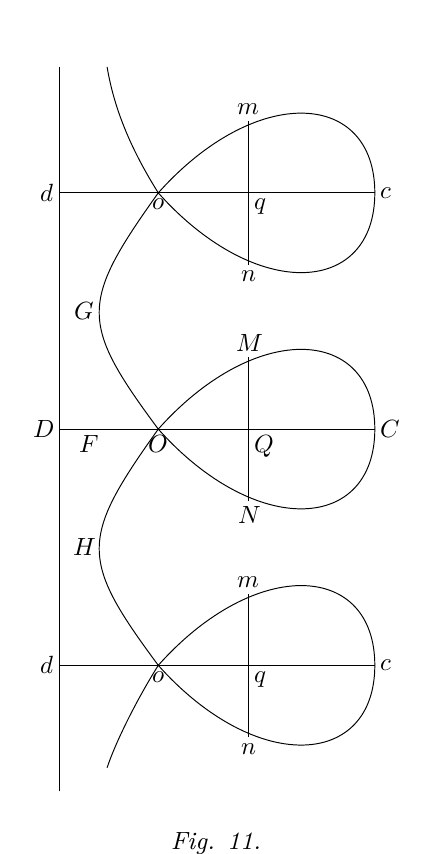
\begin{tikzpicture}[x=1cm,y=1cm,line width=.35pt,font=\small]
\draw (0,-4.6)--(0,4.6);
\draw (.6,4.6)..controls (.7,4) and (.95,3.48)..(1.25,3)..controls (2.5,1.6) and (4,1.7)..(4,3)..controls (4,4.3) and (2.5,4.4)..(1.25,3)..controls (.25,1.6) and (.25,1.35)..(1.25,0)..controls (2.5,-1.4) and (4,-1.3)..(4,0)..controls (4,1.3) and (2.5,1.4)..(1.25,0)..controls (.25,-1.4) and (.25,-1.65)..(1.25,-3)..controls (2.5,-4.4) and (4,-4.3)..(4,-3)..controls (4,-1.7) and (2.5,-1.6)..(1.25,-3)..controls (.95,-3.48) and (.7,-4)..(.6,-4.3);
\foreach \y in {-3,0,3}{\draw (0,\y)--(4,\y) (2.4,{\y-.91})--(2.4,{\y+.91});}
\node[left,inner sep=2pt] at (0,3) {$d$};
\node[below,inner sep=2pt] at (1.25,3) {$o$};
\node[right,inner sep=2pt] at (4,3) {$c$};
\node[above,inner sep=2pt] at (2.4,3.91) {$m$};
\node[below,inner sep=2pt] at (2.4,2.09) {$n$};
\node[below right,inner sep=2pt] at (2.4,3) {$q$};
\node[left,inner sep=2pt] at (0,0) {$D$};
\node[below,inner sep=2pt] at (0.35,0) {$F$};
\node[below,inner sep=2pt] at (1.25,0) {$O$};
\node[right,inner sep=2pt] at (4,0) {$C$};
\node[above,inner sep=2pt] at (2.4,0.91) {$M$};
\node[below,inner sep=2pt] at (2.4,-0.91) {$N$};
\node[below right,inner sep=2pt] at (2.4,0) {$Q$};
\node[left,inner sep=2pt] at (0.51,1.5) {$G$};
\node[left,inner sep=2pt] at (0.51,-1.5) {$H$};
\node[left,inner sep=2pt] at (0,-3) {$d$};
\node[below,inner sep=2pt] at (1.25,-3) {$o$};
\node[right,inner sep=2pt] at (4,-3) {$c$};
\node[above,inner sep=2pt] at (2.4,-2.09) {$m$};
\node[below,inner sep=2pt] at (2.4,-3.91) {$n$};
\node[below right,inner sep=2pt] at (2.4,-3) {$q$};
\node[anchor=north] at ([yshift=-4mm]current bounding box.south) {\textit{Fig. 11.}};
\end{tikzpicture}
}\end{center}
\par\bigskip
\needspace{95mm}\hypertarget{addfig:12}{}
\begin{center}\adjustbox{max width=\linewidth,max height=75mm}{% Modern editorial, markup and figure/layout contributions: CC-BY-SA-4.0.
% Historical text and illustrations: Leonhard Euler (1744), public domain.
% Component scope and upstream attribution: see RIGHTS.md.
% Manual vector redrawing after E65, Tabula IV. Schematic coordinates; original point relations retained.
\begin{tikzpicture}[x=1cm,y=1cm,line width=.35pt,font=\small]
\draw (0,-2)--(0,0)--(2.3,2.55);
\draw (0,0)..controls (1.25,1.25) and (2.65,1.35)..(3.7,.35);
\draw (0,-2.25) circle (.25);
\node[left,inner sep=2pt] at (0,0) {$A$};
\node[above,inner sep=2pt] at (2.3,2.55) {$T$};
\node[right,inner sep=2pt] at (3.7,0.35) {$C$};
\node[right,inner sep=2pt] at (0.25,-2.25) {$P$};
\node[anchor=north] at ([yshift=-4mm]current bounding box.south) {\textit{Fig. 12.}};
\end{tikzpicture}
}\end{center}
\par\bigskip
\clearpage
\needspace{95mm}\hypertarget{addfig:13}{}
\begin{center}\adjustbox{max width=\linewidth,max height=75mm}{% Modern editorial, markup and figure/layout contributions: CC-BY-SA-4.0.
% Historical text and illustrations: Leonhard Euler (1744), public domain.
% Component scope and upstream attribution: see RIGHTS.md.
% Manual vector redrawing after E65, Tabula IV. Schematic coordinates; original point relations retained.
\begin{tikzpicture}[x=1cm,y=1cm,line width=.35pt,font=\small]
\draw (-1.5,0) rectangle (1.5,.12) (-.22,.12)--(-.22,4.8) (.22,.12)--(.22,4.8);
\draw (-.52,4.8)--(.52,4.8)--(.52,4.95)..controls (.2,4.96) and (.3,5.23)..(.37,5.42)..controls (.64,6.15) and (-.64,6.15)..(-.37,5.42)..controls (-.3,5.23) and (-.2,4.96)..(-.52,4.95)--cycle;
\node[below,inner sep=2pt] at (0,0) {$A$};
\node[below right,inner sep=2pt] at (0.22,4.8) {$B$};
\node[anchor=center,inner sep=2pt] at (0,5.55) {$P$};
\node[anchor=north] at ([yshift=-4mm]current bounding box.south) {\textit{Fig. 13.}};
\end{tikzpicture}
}\end{center}
\par\bigskip
\needspace{95mm}\hypertarget{addfig:14}{}
\begin{center}\adjustbox{max width=\linewidth,max height=75mm}{% Modern editorial, markup and figure/layout contributions: CC-BY-SA-4.0.
% Historical text and illustrations: Leonhard Euler (1744), public domain.
% Component scope and upstream attribution: see RIGHTS.md.
% Manual vector redrawing after E65, Tabula IV. Schematic coordinates; original point relations retained.
\begin{tikzpicture}[x=1cm,y=1cm,line width=.35pt,font=\small]
\draw (0,-.85)--(0,0)--(5,0) (-.4,2.4)--(5,2.4) (2,0)--(2,1.61);
\draw (0,0)..controls (1.3,1.5) and (3.2,2.4)..(5,2.4);
\draw (5,0) rectangle (6.35,4.4);
\foreach \y in {.35,.7,1.05,1.4,1.75,2.1,2.45,2.8,3.15,3.5,3.85,4.2}{\draw (5,\y)--(6.35,\y);}
\foreach \y in {0,.7,1.4,2.1,2.8,3.5}{\draw (5.35,\y)--(5.35,{\y+.35}) (6,\y)--(6,{\y+.35});}
\foreach \y in {.35,1.05,1.75,2.45,3.15,3.85}{\draw (5.67,\y)--(5.67,{\y+.35});}
\draw (0,-1.15) circle (.3);
\node[left,inner sep=2pt] at (0,0) {$A$};
\node[right,inner sep=2pt] at (0.3,-1.15) {$P$};
\node[below,inner sep=2pt] at (2,0) {$p$};
\node[above,inner sep=2pt] at (2,1.61) {$m$};
\node[below,inner sep=2pt] at (5,0) {$G$};
\node[above left,inner sep=2pt] at (5,2.4) {$F$};
\node[above,inner sep=2pt] at (5.67,4.4) {$K$};
\node[above,inner sep=2pt] at (-0.4,2.4) {$H$};
\node[anchor=north] at ([yshift=-4mm]current bounding box.south) {\textit{Fig. 14.}};
\end{tikzpicture}
}\end{center}
\par\bigskip
\clearpage
\needspace{95mm}\hypertarget{addfig:15}{}
\begin{center}\adjustbox{max width=\linewidth,max height=75mm}{% Modern editorial, markup and figure/layout contributions: CC-BY-SA-4.0.
% Historical text and illustrations: Leonhard Euler (1744), public domain.
% Component scope and upstream attribution: see RIGHTS.md.
% Manual vector redrawing after E65, Tabula IV. Schematic coordinates; original point relations retained.
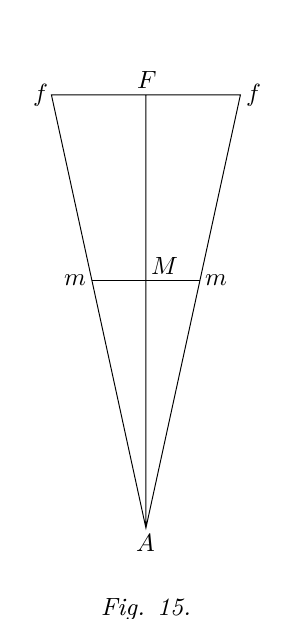
\begin{tikzpicture}[x=1cm,y=1cm,line width=.35pt,font=\small]
\draw (0,0)--(-1.2,5.5)--(1.2,5.5)--cycle (0,0)--(0,5.5) (-.6857,3.1429)--(.6857,3.1429);
\node[below,inner sep=2pt] at (0,0) {$A$};
\node[above,inner sep=2pt] at (0,5.5) {$F$};
\node[left,inner sep=2pt] at (-1.2,5.5) {$f$};
\node[right,inner sep=2pt] at (1.2,5.5) {$f$};
\node[above right,inner sep=2pt] at (0,3.1429) {$M$};
\node[left,inner sep=2pt] at (-0.6857,3.1429) {$m$};
\node[right,inner sep=2pt] at (0.6857,3.1429) {$m$};
\node[anchor=north] at ([yshift=-4mm]current bounding box.south) {\textit{Fig. 15.}};
\end{tikzpicture}
}\end{center}
\par\bigskip
\needspace{95mm}\hypertarget{addfig:16}{}
\begin{center}\adjustbox{max width=\linewidth,max height=75mm}{% Modern editorial, markup and figure/layout contributions: CC-BY-SA-4.0.
% Historical text and illustrations: Leonhard Euler (1744), public domain.
% Component scope and upstream attribution: see RIGHTS.md.
% Vector redrawing after E65, Tabula V. Schematic coordinates.
\begin{tikzpicture}[x=1cm,y=1cm,line width=.35pt,font=\small]
\draw (0,0) .. controls (1.6,2.4) and (3.4,3.7) .. (5,2.6) coordinate[pos=.7] (M);
\draw (0,0) .. controls (1.6,2.4) and (3.1,4.0) .. (4.7,4.0);
\draw (.3,2.6)--(5.6,2.6)--(5.6,1.85);
\draw (M)--(M|-0,2.6);
\draw (5.6,1.6) circle (.25);
\node[right] at (5.9,1.6) {$P$};
\node[left] at (0,0) {$B$};\node[above] at (5,2.6) {$A$};\node[above] at (5.6,2.6) {$C$};
\node[below] at (M|-0,2.6) {$P$};\node[above] at (M) {$M$};
\node[above] at (3.1,3.59) {$m$};\node[right] at (4.7,4) {$a$};
\node[anchor=north] at ([yshift=-4mm]current bounding box.south) {\textit{Fig. 16.}};
\end{tikzpicture}
}\end{center}
\par\bigskip
\clearpage
\needspace{95mm}\hypertarget{addfig:17}{}
\begin{center}\adjustbox{max width=\linewidth,max height=75mm}{% Modern editorial, markup and figure/layout contributions: CC-BY-SA-4.0.
% Historical text and illustrations: Leonhard Euler (1744), public domain.
% Component scope and upstream attribution: see RIGHTS.md.
% Vector redrawing after E65, Tabula V. Schematic coordinates.
\begin{tikzpicture}[x=1cm,y=1cm,line width=.35pt,font=\small]
\draw (0,3.8) .. controls (1.7,2.15) and (4.0,1.2) .. (6,1.2);
\draw (6,1.2)--(0,1.2)--(0,-.5);
\draw (0,-.75) circle (.25);
\node[right] at (.3,-.75) {$P$};\node[above left] at (0,3.8) {$a$};
\node[above] at (1.75,2.44) {$m$};\node[above left] at (0,1.2) {$A$};
\node[below] at (2,1.2) {$M$};\node[below right] at (6,1.2) {$B$};
\node[anchor=north] at ([yshift=-4mm]current bounding box.south) {\textit{Fig. 17.}};
\end{tikzpicture}
}\end{center}
\par\bigskip
\needspace{95mm}\hypertarget{addfig:18}{}
\begin{center}\adjustbox{max width=\linewidth,max height=75mm}{% Modern editorial, markup and figure/layout contributions: CC-BY-SA-4.0.
% Historical text and illustrations: Leonhard Euler (1744), public domain.
% Component scope and upstream attribution: see RIGHTS.md.
% Vector redrawing after E65, Tabula V. Schematic coordinates.
\begin{tikzpicture}[x=1cm,y=1cm,line width=.35pt,font=\small]
\draw (-1,0)--(5.4,0);\draw (0,0)--(0,-1);
\draw (1,0) .. controls (1,1.35) and (3.1,2.65) .. (5,3.5);
\draw (2.792,0)--(2.792,2.295)--(.5,2.295);
\draw (5,0)--(5,3.5)--(3,3.5);
\draw (3.3,2.739474)--(5.15,3.567105);\draw (5,3.5)--(5.7,1.935294);
\node[above] at (-1,0) {$F$};\node[above] at (0,0) {$C$};\node[left] at (0,-1) {$E$};
\node[below] at (1,0) {$A$};\node[below] at (2.792,0) {$p$};\node[below] at (5,0) {$P$};
\node[above left] at (2.792,2.295) {$m$};\node[below right] at (3.249,2.542) {$\mu$};
\node[left] at (.5,2.295) {$q$};\node[left] at (3,3.5) {$Q$};
\node[left] at (3.3,2.739474) {$T$};\node[above] at (5,3.5) {$M$};\node[right] at (5.7,1.935294) {$N$};
\node[anchor=north] at ([yshift=-4mm]current bounding box.south) {\textit{Fig. 18.}};
\end{tikzpicture}
}\end{center}
\par\bigskip
\clearpage
\needspace{95mm}\hypertarget{addfig:19}{}
\begin{center}\adjustbox{max width=\linewidth,max height=75mm}{% Modern editorial, markup and figure/layout contributions: CC-BY-SA-4.0.
% Historical text and illustrations: Leonhard Euler (1744), public domain.
% Component scope and upstream attribution: see RIGHTS.md.
% Vector redrawing after E65, Tabula V. Schematic coordinates.
\begin{tikzpicture}[x=1cm,y=1cm,line width=.35pt,font=\small]
\draw (0,0)--(6,0);
\draw (0,0) .. controls (2,-1.5) and (4,-1.5) .. (6,0);
\draw (1.4,0)--(1.4,-.805)--(.962,-1.9);
\node[above] at (0,0) {$A$};\node[above] at (6,0) {$B$};\node[above] at (1.4,0) {$P$};
\node[below left] at (1.4,-.805) {$M$};\node[below] at (1.9,-.974) {$m$};\node[left] at (.962,-1.9) {$N$};
\node[anchor=north] at ([yshift=-4mm]current bounding box.south) {\textit{Fig. 19.}};
\end{tikzpicture}
}\end{center}
\par\bigskip
\needspace{95mm}\hypertarget{addfig:20}{}
\begin{center}\adjustbox{max width=\linewidth,max height=75mm}{% Modern editorial, markup and figure/layout contributions: CC-BY-SA-4.0.
% Historical text and illustrations: Leonhard Euler (1744), public domain.
% Component scope and upstream attribution: see RIGHTS.md.
% Vector redrawing after E65, Tabula V. Schematic coordinates.
\begin{tikzpicture}[x=1cm,y=1cm,line width=.35pt,font=\small]
\draw (0,0)--(0,5);\draw (0,0)--(2.4,0);
\draw (0,5) .. controls (0,2.8) and (1.2,1.4) .. (2.4,0) coordinate[pos=.65] (M) coordinate[pos=.59] (m);
\draw (M-|0,0)--(M-|2.35,0);\draw (m-|0,0)--(m);
\node[left] at (0,0) {$A$};\node[left] at (0,5) {$B$};\node[right] at (2.4,0) {$a$};
\node[left] at (M-|0,0) {$P$};\node[left] at (m-|0,0) {$p$};
\node[below] at (M) {$M$};\node[above right] at (m) {$m$};\node[right] at (M-|2.35,0) {$\pi$};
\node[anchor=north] at ([yshift=-4mm]current bounding box.south) {\textit{Fig. 20.}};
\end{tikzpicture}
}\end{center}
\par\bigskip
\clearpage
\needspace{95mm}\hypertarget{addfig:21}{}
\begin{center}\adjustbox{max width=\linewidth,max height=75mm}{% Modern editorial, markup and figure/layout contributions: CC-BY-SA-4.0.
% Historical text and illustrations: Leonhard Euler (1744), public domain.
% Component scope and upstream attribution: see RIGHTS.md.
% Vector redrawing after E65, Tabula V. Schematic coordinates.
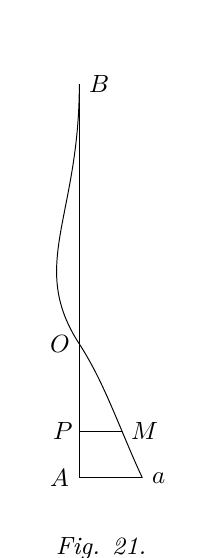
\begin{tikzpicture}[x=1cm,y=1cm,line width=.35pt,font=\small]
\draw (0,0)--(0,5);\draw (0,0)--(.8,0);
\draw (0,5) .. controls (0,3.3) and (-.65,2.7) .. (0,1.7) .. controls (.325,1.2) and (.52,.6) .. (.8,0) coordinate[pos=.67] (M);
\draw (M-|0,0)--(M);
\node[left] at (0,0) {$A$};\node[right] at (0,5) {$B$};\node[right] at (.8,0) {$a$};
\node[left] at (0,1.7) {$O$};\node[left] at (M-|0,0) {$P$};\node[right] at (M) {$M$};
\node[anchor=north] at ([yshift=-4mm]current bounding box.south) {\textit{Fig. 21.}};
\end{tikzpicture}
}\end{center}
\par\bigskip
\needspace{95mm}\hypertarget{addfig:22}{}
\begin{center}\adjustbox{max width=\linewidth,max height=75mm}{% Modern editorial, markup and figure/layout contributions: CC-BY-SA-4.0.
% Historical text and illustrations: Leonhard Euler (1744), public domain.
% Component scope and upstream attribution: see RIGHTS.md.
% Vector redrawing after E65, Tabula V. Schematic coordinates.
\begin{tikzpicture}[x=1cm,y=1cm,line width=.35pt,font=\small]
\draw (0,0)--(6,0);\draw (0,0)--(0,-.8);\draw (6,0)--(6,-.8);
\draw[domain=0:6,samples=70] plot (\x,{1-.2*(\x-3)^2});
\draw (.5,0)--(.5,-.25);\draw (3,0)--(3,1);
\node[above left] at (0,0) {$A$};\node[above] at (.5,0) {$P$};\node[below] at (.5,-.25) {$M$};
\node[below] at (.764,0) {$E$};\node[below] at (3,0) {$C$};\node[above] at (3,1) {$c$};
\node[below] at (5.236,0) {$F$};\node[above right] at (6,0) {$B$};
\node[below left] at (0,-.8) {$a$};\node[below right] at (6,-.8) {$b$};
\node[anchor=north] at ([yshift=-4mm]current bounding box.south) {\textit{Fig. 22.}};
\end{tikzpicture}
}\end{center}
\par\bigskip
\clearpage
\needspace{95mm}\hypertarget{addfig:23}{}
\begin{center}\adjustbox{max width=\linewidth,max height=75mm}{% Modern editorial, markup and figure/layout contributions: CC-BY-SA-4.0.
% Historical text and illustrations: Leonhard Euler (1744), public domain.
% Component scope and upstream attribution: see RIGHTS.md.
% Vector redrawing after E65, Tabula V. Schematic coordinates.
\begin{tikzpicture}[x=1cm,y=1cm,line width=.35pt,font=\small]
\draw (0,0)--(5,0)--(5,.65)--(0,-.65)--cycle;
\node[above left] at (0,0) {$A$};\node[below left] at (0,-.65) {$a$};
\node[below] at (2.5,0) {$C$};\node[below right] at (5,0) {$B$};\node[above right] at (5,.65) {$b$};
\node[anchor=north] at ([yshift=-4mm]current bounding box.south) {\textit{Fig. 23.}};
\end{tikzpicture}
}\end{center}
\par\bigskip
\needspace{95mm}\hypertarget{addfig:24}{}
\begin{center}\adjustbox{max width=\linewidth,max height=75mm}{% Modern editorial, markup and figure/layout contributions: CC-BY-SA-4.0.
% Historical text and illustrations: Leonhard Euler (1744), public domain.
% Component scope and upstream attribution: see RIGHTS.md.
% Vector redrawing after E65, Tabula V. Schematic coordinates.
\begin{tikzpicture}[x=1cm,y=1cm,line width=.35pt,font=\small]
\draw (0,0)--(6,0);\draw (0,-1.2)--(0,0);\draw (6,0)--(6,-1.2);
\draw (0,0) .. controls (2,1) and (4,1) .. (6,0);
\draw (1.5,0)--(1.5,1.8);
\node[left] at (0,0) {$A$};\node[right] at (6,0) {$B$};
\node[right] at (0,-1.2) {$\alpha$};\node[right] at (6,-1.2) {$\beta$};
\node[below] at (1.5,0) {$P$};\node[above left] at (1.5,.5625) {$M$};
\node[above] at (2,.667) {$m$};\node[left] at (1.5,1.8) {$\mu$};
\node[anchor=north] at ([yshift=-4mm]current bounding box.south) {\textit{Fig. 24.}};
\end{tikzpicture}
}\end{center}
\par\bigskip
\clearpage
\needspace{95mm}\hypertarget{addfig:25}{}
\begin{center}\adjustbox{max width=\linewidth,max height=75mm}{% Modern editorial, markup and figure/layout contributions: CC-BY-SA-4.0.
% Historical text and illustrations: Leonhard Euler (1744), public domain.
% Component scope and upstream attribution: see RIGHTS.md.
% Vector redrawing after E65, Tabula V. Schematic coordinates.
\begin{tikzpicture}[x=1cm,y=1cm,line width=.35pt,font=\small]
\draw (0,0)--(6,0);
\draw (0,0) .. controls (1,0) and (1.9,.75) .. (3,.75) coordinate[pos=.5] (M) .. controls (4.1,.75) and (5,0) .. (6,0);
\draw (M|-0,0)--(M);
\node[below] at (0,0) {$A$};\node[below] at (6,0) {$B$};
\node[below] at (M|-0,0) {$P$};\node[above] at (M) {$M$};
\node[anchor=north] at ([yshift=-4mm]current bounding box.south) {\textit{Fig. 25.}};
\end{tikzpicture}
}\end{center}
\par\bigskip
\needspace{95mm}\hypertarget{addfig:26}{}
\begin{center}\adjustbox{max width=\linewidth,max height=75mm}{% Modern editorial, markup and figure/layout contributions: CC-BY-SA-4.0.
% Historical text and illustrations: Leonhard Euler (1744), public domain.
% Component scope and upstream attribution: see RIGHTS.md.
% Vector redrawing after E65, Tabula V. Schematic coordinates.
\begin{tikzpicture}[x=1cm,y=1cm,line width=.35pt,font=\small]
\draw (0,-.5)--(0,4.5);
\draw[domain=0:4,samples=65] plot (\x,{3-.2*\x^2});
\draw (0,1.432)--(2.8,1.432);
\node[left] at (0,4.5) {$C$};\node[left] at (0,3) {$A$};\node[left] at (0,1.432) {$P$};
\node[above right] at (2.8,1.432) {$M$};\node[right] at (3.1,1.078) {$m$};
\node[anchor=north] at ([yshift=-4mm]current bounding box.south) {\textit{Fig. 26.}};
\end{tikzpicture}
}\end{center}
\par\bigskip
\clearpage
\needspace{95mm}\hypertarget{addfig:27}{}
\begin{center}\adjustbox{max width=\linewidth,max height=75mm}{% Modern editorial, markup and figure/layout contributions: CC-BY-SA-4.0.
% Historical text and illustrations: Leonhard Euler (1744), public domain.
% Component scope and upstream attribution: see RIGHTS.md.
% Vector redrawing after E65, Tabula V. Schematic coordinates.
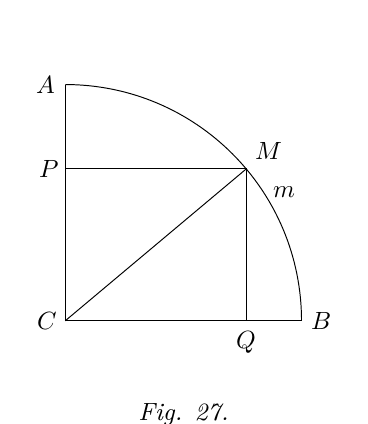
\begin{tikzpicture}[x=1cm,y=1cm,line width=.35pt,font=\small]
\draw (0,3)--(0,0)--(3,0);\draw (0,3) arc[start angle=90,end angle=0,radius=3];
\draw (0,1.92836)--(2.29813,1.92836)--(2.29813,0);\draw (0,0)--(2.29813,1.92836);
\node[left] at (0,3) {$A$};\node[left] at (0,0) {$C$};\node[right] at (3,0) {$B$};
\node[left] at (0,1.92836) {$P$};\node[below] at (2.29813,0) {$Q$};
\node[above right] at (2.29813,1.92836) {$M$};\node[right] at (2.516,1.634) {$m$};
\node[anchor=north] at ([yshift=-4mm]current bounding box.south) {\textit{Fig. 27.}};
\end{tikzpicture}
}\end{center}
\par\bigskip
\needspace{95mm}\hypertarget{addfig:28}{}
\begin{center}\adjustbox{max width=\linewidth,max height=75mm}{% Modern editorial, markup and figure/layout contributions: CC-BY-SA-4.0.
% Historical text and illustrations: Leonhard Euler (1744), public domain.
% Component scope and upstream attribution: see RIGHTS.md.
% Vector redrawing after E65, Tabula V. Circular arcs retain their centre C.
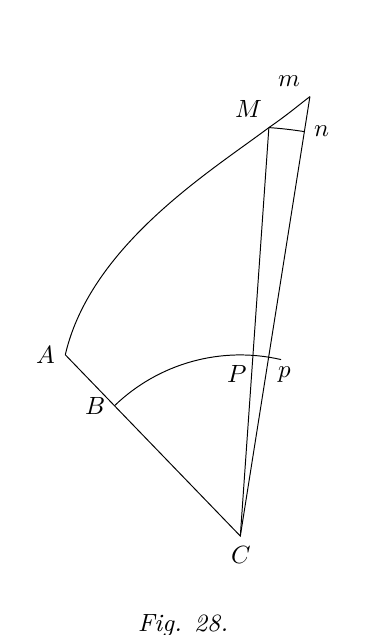
\begin{tikzpicture}[x=1cm,y=1cm,line width=.35pt,font=\small]
\coordinate (C) at (0,0);
\coordinate (A) at (134:3.2);\coordinate (B) at (134:2.3);
\coordinate (M) at (86:5.2);\coordinate (m) at (81:5.65);
\coordinate (n) at (81:5.2);\coordinate (P) at (86:2.3);\coordinate (p) at (81:2.3);
\draw (A)--(C)--(m);\draw (C)--(M);
\draw (A) .. controls (-1.9,3.7) and (-.35,4.65) .. (M) .. controls (.6,5.35) and (.75,5.48) .. (m);
\draw (B) arc[start angle=134,end angle=77,radius=2.3];
\draw (M) arc[start angle=86,end angle=81,radius=5.2];
\node[left] at (A) {$A$};\node[left] at (B) {$B$};\node[below] at (C) {$C$};
\node[above left] at (M) {$M$};\node[above left] at (m) {$m$};\node[right] at (n) {$n$};
\node[below left] at (P) {$P$};\node[below right] at (p) {$p$};
\node[anchor=north] at ([yshift=-4mm]current bounding box.south) {\textit{Fig. 28.}};
\end{tikzpicture}
}\end{center}
\par\bigskip
\clearpage
\end{document}
